\documentclass[twoside]{book}

% Packages required by doxygen
\usepackage{fixltx2e}
\usepackage{calc}
\usepackage{doxygen}
\usepackage[export]{adjustbox} % also loads graphicx
\usepackage{graphicx}
\usepackage[utf8]{inputenc}
\usepackage{makeidx}
\usepackage{multicol}
\usepackage{multirow}
\PassOptionsToPackage{warn}{textcomp}
\usepackage{textcomp}
\usepackage[nointegrals]{wasysym}
\usepackage[table]{xcolor}

% Font selection
\usepackage[T1]{fontenc}
\usepackage[scaled=.90]{helvet}
\usepackage{courier}
\usepackage{amssymb}
\usepackage{sectsty}
\renewcommand{\familydefault}{\sfdefault}
\allsectionsfont{%
  \fontseries{bc}\selectfont%
  \color{darkgray}%
}
\renewcommand{\DoxyLabelFont}{%
  \fontseries{bc}\selectfont%
  \color{darkgray}%
}
\newcommand{\+}{\discretionary{\mbox{\scriptsize$\hookleftarrow$}}{}{}}

% Page & text layout
\usepackage{geometry}
\geometry{%
  a4paper,%
  top=2.5cm,%
  bottom=2.5cm,%
  left=2.5cm,%
  right=2.5cm%
}
\tolerance=750
\hfuzz=15pt
\hbadness=750
\setlength{\emergencystretch}{15pt}
\setlength{\parindent}{0cm}
\setlength{\parskip}{3ex plus 2ex minus 2ex}
\makeatletter
\renewcommand{\paragraph}{%
  \@startsection{paragraph}{4}{0ex}{-1.0ex}{1.0ex}{%
    \normalfont\normalsize\bfseries\SS@parafont%
  }%
}
\renewcommand{\subparagraph}{%
  \@startsection{subparagraph}{5}{0ex}{-1.0ex}{1.0ex}{%
    \normalfont\normalsize\bfseries\SS@subparafont%
  }%
}
\makeatother

% Headers & footers
\usepackage{fancyhdr}
\pagestyle{fancyplain}
\fancyhead[LE]{\fancyplain{}{\bfseries\thepage}}
\fancyhead[CE]{\fancyplain{}{}}
\fancyhead[RE]{\fancyplain{}{\bfseries\leftmark}}
\fancyhead[LO]{\fancyplain{}{\bfseries\rightmark}}
\fancyhead[CO]{\fancyplain{}{}}
\fancyhead[RO]{\fancyplain{}{\bfseries\thepage}}
\fancyfoot[LE]{\fancyplain{}{}}
\fancyfoot[CE]{\fancyplain{}{}}
\fancyfoot[RE]{\fancyplain{}{\bfseries\scriptsize Generated by Doxygen }}
\fancyfoot[LO]{\fancyplain{}{\bfseries\scriptsize Generated by Doxygen }}
\fancyfoot[CO]{\fancyplain{}{}}
\fancyfoot[RO]{\fancyplain{}{}}
\renewcommand{\footrulewidth}{0.4pt}
\renewcommand{\chaptermark}[1]{%
  \markboth{#1}{}%
}
\renewcommand{\sectionmark}[1]{%
  \markright{\thesection\ #1}%
}

% Indices & bibliography
\usepackage{natbib}
\usepackage[titles]{tocloft}
\setcounter{tocdepth}{3}
\setcounter{secnumdepth}{5}
\makeindex

% Hyperlinks (required, but should be loaded last)
\usepackage{ifpdf}
\ifpdf
  \usepackage[pdftex,pagebackref=true]{hyperref}
\else
  \usepackage[ps2pdf,pagebackref=true]{hyperref}
\fi
\hypersetup{%
  colorlinks=true,%
  linkcolor=blue,%
  citecolor=blue,%
  unicode%
}

% Custom commands
\newcommand{\clearemptydoublepage}{%
  \newpage{\pagestyle{empty}\cleardoublepage}%
}

\usepackage{caption}
\captionsetup{labelsep=space,justification=centering,font={bf},singlelinecheck=off,skip=4pt,position=top}

%===== C O N T E N T S =====

\begin{document}

% Titlepage & ToC
\hypersetup{pageanchor=false,
             bookmarksnumbered=true,
             pdfencoding=unicode
            }
\pagenumbering{alph}
\begin{titlepage}
\vspace*{7cm}
\begin{center}%
{\Large My Project }\\
\vspace*{1cm}
{\large Generated by Doxygen 1.8.13}\\
\end{center}
\end{titlepage}
\clearemptydoublepage
\pagenumbering{roman}
\tableofcontents
\clearemptydoublepage
\pagenumbering{arabic}
\hypersetup{pageanchor=true}

%--- Begin generated contents ---
\chapter{R\+E\+A\+D\+ME}
\label{md_README}
\Hypertarget{md_README}


\section*{Software Básico -\/ 1/2019}

\section*{Informações}

\subsection*{Cabeçalho}


\begin{DoxyItemize}
\item 18/04/2019
\item Brasília, DF, Brasil
\item Software Básico
\item Turma\+: A -\/ 01/2019
\item Professor\+: Marcelo Ladeira
\end{DoxyItemize}

\subsection*{Autores}


\begin{DoxyItemize}
\item {\bfseries Bruno Sanguinetti R. Barros} $\vert$ {\itshape 18/0046063} $\vert$ \href{https://github.com/BrunoSNT}{\tt Git\+Hub}
\item {\bfseries Gabriel Vasconcelos} $\vert$ {\itshape 16/0120781} $\vert$ \href{https://github.com/gcvasconcelos}{\tt Git\+Hub}
\item {\bfseries Leonardo de Almeida} $\vert$ {\itshape 15/0135491} $\vert$ \href{https://github.com/leodealmeida}{\tt Git\+Hub}
\item {\bfseries Lucas Mafra} $\vert$ {\itshape 12/0126443} $\vert$ \href{https://github.com/LMafra}{\tt Git\+Hub}
\item {\bfseries Wladimir Gramacho} $\vert$ {\itshape 15/0048718} $\vert$ \href{https://github.com/wladimirgramacho}{\tt Git\+Hub}
\end{DoxyItemize}

\subsection*{Getting Started}

Essas instruções farão com que você tenha uma cópia deste projeto em sua máquina local para fins de desenvolvimento e teste.


\begin{DoxyCode}
~dir/ user$ git clone https://github.com/LMafra/sb-jvm-1-2019.git
~dir/ user$ cd sb-jvm-1-2019
\end{DoxyCode}


\subsubsection*{Compilando e Executando}

Como compilar {\ttfamily gcc -\/o main \hyperlink{main_8c}{main.\+c} reader.\+c printer.\+c instructions.\+c freemem.\+c -\/\+Wall -\/std=c99 -\/ggdb3}\+:


\begin{DoxyCode}
~dir/sb-jvm-1-2019 user$ gcc -o main main.c reader.c printer.c instructions.c freemem.c -Wall -std=c99
       -ggdb3
\end{DoxyCode}


Como executar {\ttfamily ./main}\+:


\begin{DoxyCode}
~dir/sb-jvm-1-2019 user$ ./main
\end{DoxyCode}


\subsection*{Testes}

Todos os testes foram feitos com classes fornecidas pelo professor ou baixadas da internet para fins de testes.

\subsection*{Testes de Coding Style}

Durante todo o projeto, após cada aprovaçao nos teste, foram executados os comandos 
\chapter{Class Index}
\section{Class List}
Here are the classes, structs, unions and interfaces with brief descriptions\+:\begin{DoxyCompactList}
\item\contentsline{section}{\hyperlink{structAreaMetodos}{Area\+Metodos} \\*Estrutura geral que contem todas as demais estruturas }{\pageref{structAreaMetodos}}{}
\item\contentsline{section}{\hyperlink{structAttributeInfo}{Attribute\+Info} }{\pageref{structAttributeInfo}}{}
\item\contentsline{section}{\hyperlink{classframe_1_1c}{frame\+::c} \\*Arquivo de definicao de das estruturas de um frame }{\pageref{classframe_1_1c}}{}
\item\contentsline{section}{\hyperlink{classleitor_1_1c}{leitor\+::c} \\*Define as estruturas do Classfile e as funcoes que fazem a leitura de um arquivo .class e populam as estruturas }{\pageref{classleitor_1_1c}}{}
\item\contentsline{section}{\hyperlink{classmetodo_1_1c}{metodo\+::c} \\*Define as funcoes que implementam a execucao de um metodo e instanciacao de objetos }{\pageref{classmetodo_1_1c}}{}
\item\contentsline{section}{\hyperlink{classinstrucao_1_1c}{instrucao\+::c} \\*Define, interpreta e executa as instruções do programa executado }{\pageref{classinstrucao_1_1c}}{}
\item\contentsline{section}{\hyperlink{classexibidor_1_1c}{exibidor\+::c} \\*Arquivo que exibe na tela uma estrutura \hyperlink{structClassFile}{Class\+File} imprimindo todos os dados armazenados }{\pageref{classexibidor_1_1c}}{}
\item\contentsline{section}{\hyperlink{classcarregador_1_1c}{carregador\+::c} \\*Carrega, inicializa e aloca um \hyperlink{structClassFile}{Class\+File} e associa com a estrutura do \hyperlink{structAreaMetodos}{Area\+Metodos} }{\pageref{classcarregador_1_1c}}{}
\item\contentsline{section}{\hyperlink{classdecodificador_1_1c}{decodificador\+::c} \\*Recebe uma estrutura \hyperlink{structDecodificador}{Decodificador} vazia e preenche com strings que sao as instrucoes presentes no bytecode. Retorna uma estrutura \hyperlink{structDecodificador}{Decodificador} preenchida }{\pageref{classdecodificador_1_1c}}{}
\item\contentsline{section}{\hyperlink{structClassFile}{Class\+File} }{\pageref{structClassFile}}{}
\item\contentsline{section}{\hyperlink{structCodeAttribute}{Code\+Attribute} }{\pageref{structCodeAttribute}}{}
\item\contentsline{section}{\hyperlink{structCpInfo}{Cp\+Info} }{\pageref{structCpInfo}}{}
\item\contentsline{section}{\hyperlink{structCvInfo}{Cv\+Info} }{\pageref{structCvInfo}}{}
\item\contentsline{section}{\hyperlink{structDecodificador}{Decodificador} }{\pageref{structDecodificador}}{}
\item\contentsline{section}{\hyperlink{structExceptionsAttribute}{Exceptions\+Attribute} }{\pageref{structExceptionsAttribute}}{}
\item\contentsline{section}{\hyperlink{structExceptionTable}{Exception\+Table} }{\pageref{structExceptionTable}}{}
\item\contentsline{section}{\hyperlink{structFieldInfo}{Field\+Info} }{\pageref{structFieldInfo}}{}
\item\contentsline{section}{\hyperlink{structFrame}{Frame} }{\pageref{structFrame}}{}
\item\contentsline{section}{\hyperlink{structMethodInfo}{Method\+Info} }{\pageref{structMethodInfo}}{}
\item\contentsline{section}{\hyperlink{structObjeto}{Objeto} \\*Estrutura para um objeto java }{\pageref{structObjeto}}{}
\item\contentsline{section}{\hyperlink{structPilhaOp}{Pilha\+Op} }{\pageref{structPilhaOp}}{}
\item\contentsline{section}{\hyperlink{structStackFrame}{Stack\+Frame} }{\pageref{structStackFrame}}{}
\item\contentsline{section}{\hyperlink{structVector}{Vector} }{\pageref{structVector}}{}
\end{DoxyCompactList}

\chapter{File Index}
\doxysection{Lista de ficheiros}
Lista de todos os ficheiros documentados com uma breve descrição\+:\begin{DoxyCompactList}
\item\contentsline{section}{\mbox{\hyperlink{main_8c}{main.\+c}} \\*Responsável pelo processamento do arquivo .class e execução das instruções da J\+VM }{\pageref{main_8c}}{}
\item\contentsline{section}{\mbox{\hyperlink{printer_8c}{printer.\+c}} \\*Responsavel por imprimir no terminal a estrutura do classfile lido. ~\newline
}{\pageref{printer_8c}}{}
\item\contentsline{section}{\mbox{\hyperlink{printer_8h}{printer.\+h}} \\*Cabeçalho do exibidor do classfile no terminal. ~\newline
}{\pageref{printer_8h}}{}
\item\contentsline{section}{\mbox{\hyperlink{reader_8c}{reader.\+c}} \\*Responsavel por ler o .class e montar as estruturas. ~\newline
}{\pageref{reader_8c}}{}
\item\contentsline{section}{\mbox{\hyperlink{reader_8h}{reader.\+h}} \\*Cabeçalho do leitor do .class. ~\newline
}{\pageref{reader_8h}}{}
\end{DoxyCompactList}

\chapter{Class Documentation}
\hypertarget{structAreaMetodos}{}\section{Area\+Metodos Struct Reference}
\label{structAreaMetodos}\index{Area\+Metodos@{Area\+Metodos}}


Estrutura geral que contem todas as demais estruturas.  




{\ttfamily \#include $<$area\+Metodos.\+h$>$}



Collaboration diagram for Area\+Metodos\+:
% FIG 0
\subsection*{Public Attributes}
\begin{DoxyCompactItemize}
\item 
\mbox{\Hypertarget{structAreaMetodos_a2f53ae03ffa9b13b9866efb46811c988}\label{structAreaMetodos_a2f53ae03ffa9b13b9866efb46811c988}} 
\hyperlink{structClassFile}{Class\+File} $\ast$$\ast$ {\bfseries array\+Classes}
\item 
\mbox{\Hypertarget{structAreaMetodos_a16f79347136c9dda54c97a62bd596887}\label{structAreaMetodos_a16f79347136c9dda54c97a62bd596887}} 
int {\bfseries num\+Classes}
\end{DoxyCompactItemize}


\subsection{Detailed Description}
Estrutura geral que contem todas as demais estruturas. 

Aqui ficam guaradas as classes carregadas e todas as subestrutures dessas classes. 

The documentation for this struct was generated from the following file\+:\begin{DoxyCompactItemize}
\item 
\hyperlink{areaMetodos_8h}{area\+Metodos.\+h}\end{DoxyCompactItemize}

\hypertarget{structAttributeInfo}{}\section{Attribute\+Info Struct Reference}
\label{structAttributeInfo}\index{AttributeInfo@{AttributeInfo}}
\subsection*{Public Attributes}
\begin{DoxyCompactItemize}
\item 
\mbox{\Hypertarget{structAttributeInfo_ac0d9d9ffa3214f362c4e06df78036d6e}\label{structAttributeInfo_ac0d9d9ffa3214f362c4e06df78036d6e}} 
uint16\+\_\+t {\bfseries attribute\+Name\+Index}
\item 
\mbox{\Hypertarget{structAttributeInfo_a1755dec7721e0e62a53c698831ba514d}\label{structAttributeInfo_a1755dec7721e0e62a53c698831ba514d}} 
uint32\+\_\+t {\bfseries attribute\+Length}
\item 
\mbox{\Hypertarget{structAttributeInfo_a29031abd0ae7fd3a55950616e5368dd2}\label{structAttributeInfo_a29031abd0ae7fd3a55950616e5368dd2}} 
uint8\+\_\+t $\ast$ {\bfseries info}
\end{DoxyCompactItemize}


The documentation for this struct was generated from the following file\+:\begin{DoxyCompactItemize}
\item 
\mbox{\hyperlink{leitor_8h}{leitor.\+h}}\end{DoxyCompactItemize}

\hypertarget{classframe_1_1c}{}\section{frame\+:\+:c Class Reference}
\label{classframe_1_1c}\index{frame\+::c@{frame\+::c}}


Arquivo de definicao de das estruturas de um frame.  




{\ttfamily \#include \char`\"{}leitor.\+h\char`\"{}}



\subsection{Detailed Description}
Arquivo de definicao de das estruturas de um frame. 

\begin{DoxyDate}{Date}
26/06/17. 
\end{DoxyDate}
\begin{DoxyCopyright}{Copyright}
Copyright © 2017 Grupo\+SB. All rights reserved.
\end{DoxyCopyright}
\begin{DoxyAuthor}{Authors}
Bruno Sanguinetti 18/0046063 ~\newline
Gabriel Vasconcelos 16/0120781 ~\newline
Leonardo de Almeida 15/0135491 ~\newline
Lucas Mafra 12/0126443 ~\newline
Wladimir Gramacho 15/0058718 ~\newline

\end{DoxyAuthor}


The documentation for this class was generated from the following file\+:\begin{DoxyCompactItemize}
\item 
\hyperlink{frame_8h}{frame.\+h}\end{DoxyCompactItemize}

\hypertarget{classleitor_1_1c}{}\section{leitor\+::c Class Reference}
\label{classleitor_1_1c}\index{leitor::c@{leitor::c}}


Define as estruturas do Classfile e as funcoes que fazem a leitura de um arquivo .class e populam as estruturas.  




{\ttfamily \#include \char`\"{}decodificador.\+h\char`\"{}}



\subsection{Detailed Description}
Define as estruturas do Classfile e as funcoes que fazem a leitura de um arquivo .class e populam as estruturas. 

\begin{DoxyDate}{Date}
28/06/19.
\end{DoxyDate}
\begin{DoxyAuthor}{Authors}
Bruno Sanguinetti 18/0046063 ~\newline
Gabriel Vasconcelos 16/0120781 ~\newline
Leonardo de Almeida 15/0135491 ~\newline
Lucas Mafra 12/0126443 ~\newline
Wladimir Gramacho 15/0058718 ~\newline

\end{DoxyAuthor}


The documentation for this class was generated from the following file\+:\begin{DoxyCompactItemize}
\item 
\mbox{\hyperlink{leitor_8h}{leitor.\+h}}\end{DoxyCompactItemize}

\hypertarget{classmetodo_1_1c}{}\section{metodo\+:\+:c Class Reference}
\label{classmetodo_1_1c}\index{metodo\+::c@{metodo\+::c}}


Define as funcoes que implementam a execucao de um metodo e instanciacao de objetos.  




{\ttfamily \#include \char`\"{}carregador.\+h\char`\"{}}



\subsection{Detailed Description}
Define as funcoes que implementam a execucao de um metodo e instanciacao de objetos. 

\begin{DoxyDate}{Date}
28/06/19.
\end{DoxyDate}
\begin{DoxyAuthor}{Authors}
Bruno Sanguinetti 18/0046063 ~\newline
Gabriel Vasconcelos 16/0120781 ~\newline
Leonardo de Almeida 15/0135491 ~\newline
Lucas Mafra 12/0126443 ~\newline
Wladimir Gramacho 15/0058718 ~\newline

\end{DoxyAuthor}


The documentation for this class was generated from the following file\+:\begin{DoxyCompactItemize}
\item 
\hyperlink{metodo_8h}{metodo.\+h}\end{DoxyCompactItemize}

\hypertarget{classinstrucao_1_1c}{}\section{instrucao\+:\+:c Class Reference}
\label{classinstrucao_1_1c}\index{instrucao\+::c@{instrucao\+::c}}


Define, interpreta e executa as instruções do programa executado.  




{\ttfamily \#include \char`\"{}instrucao.\+c\char`\"{}}



\subsection{Detailed Description}
Define, interpreta e executa as instruções do programa executado. 

\begin{DoxyDate}{Date}
28/06/19.
\end{DoxyDate}
\begin{DoxyAuthor}{Authors}
Bruno Sanguinetti 18/0046063 ~\newline
Gabriel Vasconcelos 16/0120781 ~\newline
Leonardo de Almeida 15/0135491 ~\newline
Lucas Mafra 12/0126443 ~\newline
Wladimir Gramacho 15/0058718 ~\newline

\end{DoxyAuthor}


The documentation for this class was generated from the following file\+:\begin{DoxyCompactItemize}
\item 
\hyperlink{instrucao_8h}{instrucao.\+h}\end{DoxyCompactItemize}

\hypertarget{classexibidor_1_1c}{}\section{exibidor\+:\+:c Class Reference}
\label{classexibidor_1_1c}\index{exibidor\+::c@{exibidor\+::c}}


Arquivo que exibe na tela uma estrutura \hyperlink{structClassFile}{Class\+File} imprimindo todos os dados armazenados.  




{\ttfamily \#include \char`\"{}leitor.\+h\char`\"{}}



\subsection{Detailed Description}
Arquivo que exibe na tela uma estrutura \hyperlink{structClassFile}{Class\+File} imprimindo todos os dados armazenados. 

\begin{DoxyDate}{Date}
28/06/17. 
\end{DoxyDate}
\begin{DoxyCopyright}{Copyright}
Copyright © 2017 Grupo\+SB. All rights reserved.
\end{DoxyCopyright}
\begin{DoxyAuthor}{Authors}
Bruno Sanguinetti 18/0046063 ~\newline
Gabriel Vasconcelos 16/0120781 ~\newline
Leonardo de Almeida 15/0135491 ~\newline
Lucas Mafra 12/0126443 ~\newline
Wladimir Gramacho 15/0058718 ~\newline
 Recebe um ponteiro para uma estrutura \hyperlink{structClassFile}{Class\+File}, imprime cada parte de acordo com seu formato e suas subestruturas, isso tudo com uma interface semelhante ao programa \char`\"{}jclasslib bytecode viewer\char`\"{}. 
\end{DoxyAuthor}


The documentation for this class was generated from the following file\+:\begin{DoxyCompactItemize}
\item 
\hyperlink{exibidor_8h}{exibidor.\+h}\end{DoxyCompactItemize}

\hypertarget{classcarregador_1_1c}{}\section{carregador\+:\+:c Class Reference}
\label{classcarregador_1_1c}\index{carregador\+::c@{carregador\+::c}}


Carrega, inicializa e aloca um \hyperlink{structClassFile}{Class\+File} e associa com a estrutura do \hyperlink{structAreaMetodos}{Area\+Metodos}.  




{\ttfamily \#include \char`\"{}area\+Metodos.\+h\char`\"{}}



\subsection{Detailed Description}
Carrega, inicializa e aloca um \hyperlink{structClassFile}{Class\+File} e associa com a estrutura do \hyperlink{structAreaMetodos}{Area\+Metodos}. 

\begin{DoxyDate}{Date}
28/06/17. 
\end{DoxyDate}
\begin{DoxyCopyright}{Copyright}
Copyright © 2017 Grupo\+SB. All rights reserved.
\end{DoxyCopyright}
\begin{DoxyAuthor}{Authors}
Bruno Sanguinetti 18/0046063 ~\newline
Gabriel Vasconcelos 16/0120781 ~\newline
Leonardo de Almeida 15/0135491 ~\newline
Lucas Mafra 12/0126443 ~\newline
Wladimir Gramacho 15/0058718 ~\newline

\end{DoxyAuthor}


The documentation for this class was generated from the following file\+:\begin{DoxyCompactItemize}
\item 
\hyperlink{carregador_8h}{carregador.\+h}\end{DoxyCompactItemize}

\hypertarget{classdecodificador_1_1c}{}\section{decodificador\+::c Class Reference}
\label{classdecodificador_1_1c}\index{decodificador::c@{decodificador::c}}


Recebe uma estrutura \mbox{\hyperlink{structDecodificador}{Decodificador}} vazia e preenche com strings que sao as instrucoes presentes no bytecode. Retorna uma estrutura \mbox{\hyperlink{structDecodificador}{Decodificador}} preenchida.  




{\ttfamily \#include \char`\"{}decodificador.\+c\char`\"{}}



\subsection{Detailed Description}
Recebe uma estrutura \mbox{\hyperlink{structDecodificador}{Decodificador}} vazia e preenche com strings que sao as instrucoes presentes no bytecode. Retorna uma estrutura \mbox{\hyperlink{structDecodificador}{Decodificador}} preenchida. 

\begin{DoxyDate}{Date}
26/07/2019.
\end{DoxyDate}
\begin{DoxyAuthor}{Authors}
Bruno Sanguinetti 18/0046063 ~\newline
Gabriel Vasconcelos 16/0120781 ~\newline
Leonardo de Almeida 15/0135491 ~\newline
Lucas Mafra 12/0126443 ~\newline
Wladimir Gramacho 15/0058718 ~\newline

\end{DoxyAuthor}


The documentation for this class was generated from the following file\+:\begin{DoxyCompactItemize}
\item 
\mbox{\hyperlink{decodificador_8h}{decodificador.\+h}}\end{DoxyCompactItemize}

\hypertarget{structClassFile}{}\section{Class\+File Struct Reference}
\label{structClassFile}\index{Class\+File@{Class\+File}}


Collaboration diagram for Class\+File\+:
% FIG 0
\subsection*{Public Attributes}
\begin{DoxyCompactItemize}
\item 
\mbox{\Hypertarget{structClassFile_a9d4d72751ff9250dd3305d5d853f7921}\label{structClassFile_a9d4d72751ff9250dd3305d5d853f7921}} 
uint32\+\_\+t {\bfseries magic}
\item 
\mbox{\Hypertarget{structClassFile_afb41e706bd0e19ed5a24cd0e99ecc4c1}\label{structClassFile_afb41e706bd0e19ed5a24cd0e99ecc4c1}} 
uint16\+\_\+t {\bfseries minor\+Version}
\item 
\mbox{\Hypertarget{structClassFile_a3424e098e9ef6dbfbdbb9c708afaffe7}\label{structClassFile_a3424e098e9ef6dbfbdbb9c708afaffe7}} 
uint16\+\_\+t {\bfseries major\+Version}
\item 
\mbox{\Hypertarget{structClassFile_af185527e4689b1672655f608df4a3c62}\label{structClassFile_af185527e4689b1672655f608df4a3c62}} 
uint16\+\_\+t {\bfseries constant\+Pool\+Count}
\item 
\mbox{\Hypertarget{structClassFile_a209de5f28c80fb453b37a3f0b320ab9c}\label{structClassFile_a209de5f28c80fb453b37a3f0b320ab9c}} 
\hyperlink{structCpInfo}{Cp\+Info} $\ast$ {\bfseries constant\+Pool}
\item 
\mbox{\Hypertarget{structClassFile_afbb2cd57bb6eb5baa34e83127e928c18}\label{structClassFile_afbb2cd57bb6eb5baa34e83127e928c18}} 
uint16\+\_\+t {\bfseries access\+Flags}
\item 
\mbox{\Hypertarget{structClassFile_abc02e661935c638b2f231cef576859f1}\label{structClassFile_abc02e661935c638b2f231cef576859f1}} 
uint16\+\_\+t {\bfseries this\+Class}
\item 
\mbox{\Hypertarget{structClassFile_a306c9da73620fa5ad94bbaa64a19afdd}\label{structClassFile_a306c9da73620fa5ad94bbaa64a19afdd}} 
uint16\+\_\+t {\bfseries super\+Class}
\item 
\mbox{\Hypertarget{structClassFile_adcd02751a38d5b17559fd3c5201b2c42}\label{structClassFile_adcd02751a38d5b17559fd3c5201b2c42}} 
uint16\+\_\+t {\bfseries interfaces\+Count}
\item 
\mbox{\Hypertarget{structClassFile_a86680de028c6df386edafa8e8436b92c}\label{structClassFile_a86680de028c6df386edafa8e8436b92c}} 
uint16\+\_\+t $\ast$ {\bfseries interfaces}
\item 
\mbox{\Hypertarget{structClassFile_a87f4d2ede2eb9df54d69952df84226ca}\label{structClassFile_a87f4d2ede2eb9df54d69952df84226ca}} 
uint16\+\_\+t {\bfseries fields\+Count}
\item 
\mbox{\Hypertarget{structClassFile_add171dc12613ad29ef94f4f18a50f06a}\label{structClassFile_add171dc12613ad29ef94f4f18a50f06a}} 
\hyperlink{structFieldInfo}{Field\+Info} $\ast$ {\bfseries fields}
\item 
\mbox{\Hypertarget{structClassFile_a24d224be2ab473bac3506890c6ff6a4d}\label{structClassFile_a24d224be2ab473bac3506890c6ff6a4d}} 
uint16\+\_\+t {\bfseries methods\+Count}
\item 
\mbox{\Hypertarget{structClassFile_a67e02d50e6807bb97d7d8f265deef9a0}\label{structClassFile_a67e02d50e6807bb97d7d8f265deef9a0}} 
\hyperlink{structMethodInfo}{Method\+Info} $\ast$ {\bfseries methods}
\item 
\mbox{\Hypertarget{structClassFile_ad88c9b8262fbd79d49ad2c163ad45716}\label{structClassFile_ad88c9b8262fbd79d49ad2c163ad45716}} 
uint16\+\_\+t {\bfseries attributes\+Count}
\item 
\mbox{\Hypertarget{structClassFile_ad7db56de00dc682671cb8cfb837d92b7}\label{structClassFile_ad7db56de00dc682671cb8cfb837d92b7}} 
\hyperlink{structAttributeInfo}{Attribute\+Info} $\ast$ {\bfseries attributes}
\end{DoxyCompactItemize}


The documentation for this struct was generated from the following file\+:\begin{DoxyCompactItemize}
\item 
\hyperlink{leitor_8h}{leitor.\+h}\end{DoxyCompactItemize}

\hypertarget{structCodeAttribute}{}\section{Code\+Attribute Struct Reference}
\label{structCodeAttribute}\index{Code\+Attribute@{Code\+Attribute}}


Collaboration diagram for Code\+Attribute\+:
% FIG 0
\subsection*{Public Attributes}
\begin{DoxyCompactItemize}
\item 
\mbox{\Hypertarget{structCodeAttribute_ad7ee24e03606191ad3f75e919e10d314}\label{structCodeAttribute_ad7ee24e03606191ad3f75e919e10d314}} 
uint16\+\_\+t {\bfseries attribute\+Name\+Index}
\item 
\mbox{\Hypertarget{structCodeAttribute_ad7847fdf04ce98313bf197308db2f3eb}\label{structCodeAttribute_ad7847fdf04ce98313bf197308db2f3eb}} 
uint32\+\_\+t {\bfseries attribute\+Length}
\item 
\mbox{\Hypertarget{structCodeAttribute_a909f0678f0621617233e76073a55976a}\label{structCodeAttribute_a909f0678f0621617233e76073a55976a}} 
uint16\+\_\+t {\bfseries max\+Stack}
\item 
\mbox{\Hypertarget{structCodeAttribute_a8fe52af0bc8aa61d0dbeb8a3a9233731}\label{structCodeAttribute_a8fe52af0bc8aa61d0dbeb8a3a9233731}} 
uint16\+\_\+t {\bfseries max\+Locals}
\item 
\mbox{\Hypertarget{structCodeAttribute_a56ef08dd29653bdfd922f59dbf3ca619}\label{structCodeAttribute_a56ef08dd29653bdfd922f59dbf3ca619}} 
uint32\+\_\+t {\bfseries code\+Length}
\item 
\mbox{\Hypertarget{structCodeAttribute_a95d8e9c3e0b93220defcbc9852ec6c27}\label{structCodeAttribute_a95d8e9c3e0b93220defcbc9852ec6c27}} 
uint8\+\_\+t $\ast$ {\bfseries code}
\item 
\mbox{\Hypertarget{structCodeAttribute_adcab31464c6fcea300f5fd171c536591}\label{structCodeAttribute_adcab31464c6fcea300f5fd171c536591}} 
uint16\+\_\+t {\bfseries exception\+Table\+Length}
\item 
\mbox{\Hypertarget{structCodeAttribute_a59ef2cc9a1890d0fd0436278ef14c87a}\label{structCodeAttribute_a59ef2cc9a1890d0fd0436278ef14c87a}} 
\hyperlink{structExceptionTable}{Exception\+Table} $\ast$ {\bfseries exception\+Table}
\item 
\mbox{\Hypertarget{structCodeAttribute_ae76ef93751db55059ac434e073178f83}\label{structCodeAttribute_ae76ef93751db55059ac434e073178f83}} 
uint16\+\_\+t {\bfseries attributes\+Count}
\item 
\mbox{\Hypertarget{structCodeAttribute_a99297a4945c876dd5615d84986043c21}\label{structCodeAttribute_a99297a4945c876dd5615d84986043c21}} 
\hyperlink{structAttributeInfo}{Attribute\+Info} $\ast$ {\bfseries attributes}
\end{DoxyCompactItemize}


The documentation for this struct was generated from the following file\+:\begin{DoxyCompactItemize}
\item 
\hyperlink{leitor_8h}{leitor.\+h}\end{DoxyCompactItemize}

\hypertarget{structCpInfo}{}\section{Cp\+Info Struct Reference}
\label{structCpInfo}\index{Cp\+Info@{Cp\+Info}}
\subsection*{Public Attributes}
\begin{DoxyCompactItemize}
\item 
\mbox{\Hypertarget{structCpInfo_ac20d96c33f871bde2e903708a215a2dc}\label{structCpInfo_ac20d96c33f871bde2e903708a215a2dc}} 
uint8\+\_\+t {\bfseries tag}
\item 
\mbox{\Hypertarget{structCpInfo_a67bf62f1bfb88277813bff0a1524a854}\label{structCpInfo_a67bf62f1bfb88277813bff0a1524a854}} 
\begin{tabbing}
xx\=xx\=xx\=xx\=xx\=xx\=xx\=xx\=xx\=\kill
union \{\\
\>struct \{\\
\>\>uint16\_t {\bfseries nameIndex}\\
\>\} {\bfseries Class}\\
\>struct \{\\
\>\>uint16\_t {\bfseries classIndex}\\
\>\>uint16\_t {\bfseries nameAndTypeIndex}\\
\>\} {\bfseries Fieldref}\\
\>struct \{\\
\>\>uint16\_t {\bfseries classIndex}\\
\>\>uint16\_t {\bfseries nameAndTypeIndex}\\
\>\} {\bfseries Methodref}\\
\>struct \{\\
\>\>uint16\_t {\bfseries classIndex}\\
\>\>uint16\_t {\bfseries nameAndTypeIndex}\\
\>\} {\bfseries InterfaceMethodref}\\
\>struct \{\\
\>\>uint16\_t {\bfseries stringIndex}\\
\>\} {\bfseries String}\\
\>struct \{\\
\>\>uint32\_t {\bfseries bytes}\\
\>\} {\bfseries Integer}\\
\>struct \{\\
\>\>uint32\_t {\bfseries bytes}\\
\>\} {\bfseries Float}\\
\>struct \{\\
\>\>uint32\_t {\bfseries highBytes}\\
\>\>uint32\_t {\bfseries lowBytes}\\
\>\} {\bfseries Long}\\
\>struct \{\\
\>\>uint32\_t {\bfseries highBytes}\\
\>\>uint32\_t {\bfseries lowBytes}\\
\>\} {\bfseries Double}\\
\>struct \{\\
\>\>uint16\_t {\bfseries nameIndex}\\
\>\>uint16\_t {\bfseries descriptorIndex}\\
\>\} {\bfseries NameAndType}\\
\>struct \{\\
\>\>uint16\_t {\bfseries length}\\
\>\>uint8\_t $\ast$ {\bfseries bytes}\\
\>\} {\bfseries Utf8}\\
\} {\bfseries info}\\

\end{tabbing}\end{DoxyCompactItemize}


The documentation for this struct was generated from the following file\+:\begin{DoxyCompactItemize}
\item 
\hyperlink{leitor_8h}{leitor.\+h}\end{DoxyCompactItemize}

\hypertarget{structCvInfo}{}\section{Cv\+Info Struct Reference}
\label{structCvInfo}\index{CvInfo@{CvInfo}}
\subsection*{Public Attributes}
\begin{DoxyCompactItemize}
\item 
\mbox{\Hypertarget{structCvInfo_ab33f866a4dfccc3684b00cadde84aec4}\label{structCvInfo_ab33f866a4dfccc3684b00cadde84aec4}} 
uint16\+\_\+t {\bfseries attribute\+Name\+Index}
\item 
\mbox{\Hypertarget{structCvInfo_a58d31f430ddf05c081616479997ebf34}\label{structCvInfo_a58d31f430ddf05c081616479997ebf34}} 
uint32\+\_\+t {\bfseries attribute\+Length}
\item 
\mbox{\Hypertarget{structCvInfo_a44e05b3248c82f0c649a36cd66098e4c}\label{structCvInfo_a44e05b3248c82f0c649a36cd66098e4c}} 
uint16\+\_\+t {\bfseries constant\+Value\+Index}
\end{DoxyCompactItemize}


The documentation for this struct was generated from the following file\+:\begin{DoxyCompactItemize}
\item 
\mbox{\hyperlink{leitor_8h}{leitor.\+h}}\end{DoxyCompactItemize}

\hypertarget{structDecodificador}{}\section{Decodificador Struct Reference}
\label{structDecodificador}\index{Decodificador@{Decodificador}}
\subsection*{Public Attributes}
\begin{DoxyCompactItemize}
\item 
\mbox{\Hypertarget{structDecodificador_abd91e4ab4dc0ec38489f2c487132ccff}\label{structDecodificador_abd91e4ab4dc0ec38489f2c487132ccff}} 
char {\bfseries instrucao} \mbox{[}N\+O\+M\+E\+\_\+\+I\+N\+S\+T\+R\+U\+C\+AO\mbox{]}
\item 
\mbox{\Hypertarget{structDecodificador_a7081a89f9d4428ef33fb56f647363f72}\label{structDecodificador_a7081a89f9d4428ef33fb56f647363f72}} 
int {\bfseries bytes}
\end{DoxyCompactItemize}


The documentation for this struct was generated from the following file\+:\begin{DoxyCompactItemize}
\item 
\hyperlink{decodificador_8h}{decodificador.\+h}\end{DoxyCompactItemize}

\hypertarget{structExceptionsAttribute}{}\section{Exceptions\+Attribute Struct Reference}
\label{structExceptionsAttribute}\index{ExceptionsAttribute@{ExceptionsAttribute}}
\subsection*{Public Attributes}
\begin{DoxyCompactItemize}
\item 
\mbox{\Hypertarget{structExceptionsAttribute_a18fa6a96d9f0c1a55230e688d72b2a4c}\label{structExceptionsAttribute_a18fa6a96d9f0c1a55230e688d72b2a4c}} 
uint16\+\_\+t {\bfseries attribute\+Name\+Index}
\item 
\mbox{\Hypertarget{structExceptionsAttribute_ab2bca3da1eb560c5c08449106ff85c54}\label{structExceptionsAttribute_ab2bca3da1eb560c5c08449106ff85c54}} 
uint32\+\_\+t {\bfseries attribute\+Length}
\item 
\mbox{\Hypertarget{structExceptionsAttribute_ae877887aa7835d6a65b2a9dcf313e849}\label{structExceptionsAttribute_ae877887aa7835d6a65b2a9dcf313e849}} 
uint16\+\_\+t {\bfseries number\+Exceptions}
\item 
\mbox{\Hypertarget{structExceptionsAttribute_a6e7edf18fe9cf9f9cae4e4aed16d0837}\label{structExceptionsAttribute_a6e7edf18fe9cf9f9cae4e4aed16d0837}} 
uint16\+\_\+t $\ast$ {\bfseries exception\+Index\+Table}
\end{DoxyCompactItemize}


The documentation for this struct was generated from the following file\+:\begin{DoxyCompactItemize}
\item 
\mbox{\hyperlink{leitor_8h}{leitor.\+h}}\end{DoxyCompactItemize}

\hypertarget{structExceptionTable}{}\section{Exception\+Table Struct Reference}
\label{structExceptionTable}\index{Exception\+Table@{Exception\+Table}}
\subsection*{Public Attributes}
\begin{DoxyCompactItemize}
\item 
\mbox{\Hypertarget{structExceptionTable_a04ab9fcb6779181df0079a864f442e15}\label{structExceptionTable_a04ab9fcb6779181df0079a864f442e15}} 
uint16\+\_\+t {\bfseries start\+Pc}
\item 
\mbox{\Hypertarget{structExceptionTable_a89792e3b2a4737f8f2441fed7ec15aac}\label{structExceptionTable_a89792e3b2a4737f8f2441fed7ec15aac}} 
uint16\+\_\+t {\bfseries end\+Pc}
\item 
\mbox{\Hypertarget{structExceptionTable_ac9dbcf3326262a17a88c1ed875d6459f}\label{structExceptionTable_ac9dbcf3326262a17a88c1ed875d6459f}} 
uint16\+\_\+t {\bfseries catch\+Type}
\end{DoxyCompactItemize}


The documentation for this struct was generated from the following file\+:\begin{DoxyCompactItemize}
\item 
\hyperlink{leitor_8h}{leitor.\+h}\end{DoxyCompactItemize}

\hypertarget{structFieldInfo}{}\section{Field\+Info Struct Reference}
\label{structFieldInfo}\index{Field\+Info@{Field\+Info}}


Collaboration diagram for Field\+Info\+:
% FIG 0
\subsection*{Public Attributes}
\begin{DoxyCompactItemize}
\item 
\mbox{\Hypertarget{structFieldInfo_a5fd94bd00a430098ff830c231d3f7a53}\label{structFieldInfo_a5fd94bd00a430098ff830c231d3f7a53}} 
uint16\+\_\+t {\bfseries access\+Flags}
\item 
\mbox{\Hypertarget{structFieldInfo_a88ea5c29063df8933d5277e846924b1e}\label{structFieldInfo_a88ea5c29063df8933d5277e846924b1e}} 
uint16\+\_\+t {\bfseries name\+Index}
\item 
\mbox{\Hypertarget{structFieldInfo_ab6cc30d06db3569171dd6fdcba7add29}\label{structFieldInfo_ab6cc30d06db3569171dd6fdcba7add29}} 
uint16\+\_\+t {\bfseries descriptor\+Index}
\item 
\mbox{\Hypertarget{structFieldInfo_ad8eae2b3a0fccae8700ca53263983c6e}\label{structFieldInfo_ad8eae2b3a0fccae8700ca53263983c6e}} 
uint16\+\_\+t {\bfseries attributes\+Count}
\item 
\mbox{\Hypertarget{structFieldInfo_a44bc588a62523995db41f7186d6d4253}\label{structFieldInfo_a44bc588a62523995db41f7186d6d4253}} 
\hyperlink{structCvInfo}{Cv\+Info} $\ast$ {\bfseries attributes}
\end{DoxyCompactItemize}


The documentation for this struct was generated from the following file\+:\begin{DoxyCompactItemize}
\item 
\hyperlink{leitor_8h}{leitor.\+h}\end{DoxyCompactItemize}

\hypertarget{structFrame}{}\section{Frame Struct Reference}
\label{structFrame}\index{Frame@{Frame}}


Collaboration diagram for Frame\+:
\nopagebreak
\begin{figure}[H]
\begin{center}
\leavevmode
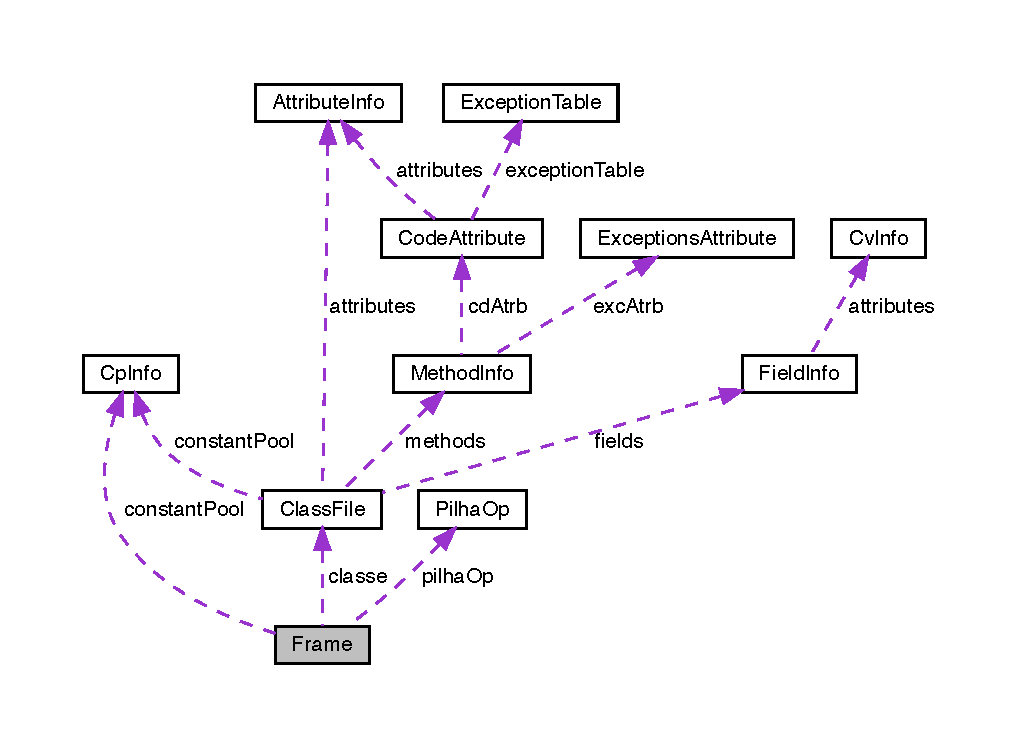
\includegraphics[width=350pt]{structFrame__coll__graph}
\end{center}
\end{figure}
\subsection*{Public Attributes}
\begin{DoxyCompactItemize}
\item 
\mbox{\Hypertarget{structFrame_a9047c9524d44fc81cb6311de8a2a8b77}\label{structFrame_a9047c9524d44fc81cb6311de8a2a8b77}} 
int32\+\_\+t $\ast$ {\bfseries local\+Variables}
\item 
\mbox{\Hypertarget{structFrame_a8067fdcfa9b9b35c39434ed4689b3aea}\label{structFrame_a8067fdcfa9b9b35c39434ed4689b3aea}} 
\mbox{\hyperlink{structCpInfo}{Cp\+Info}} $\ast$ {\bfseries constant\+Pool}
\item 
\mbox{\Hypertarget{structFrame_a3ce27d5278d61a0abaeca31956febc1f}\label{structFrame_a3ce27d5278d61a0abaeca31956febc1f}} 
\mbox{\hyperlink{structClassFile}{Class\+File}} $\ast$ {\bfseries classe}
\item 
\mbox{\Hypertarget{structFrame_a378c00e14ef1f63cbbfa4e984502b652}\label{structFrame_a378c00e14ef1f63cbbfa4e984502b652}} 
uint16\+\_\+t {\bfseries max\+Stack}
\item 
\mbox{\Hypertarget{structFrame_a5d933cb41bf8f544aecba4ef1723ab1a}\label{structFrame_a5d933cb41bf8f544aecba4ef1723ab1a}} 
uint16\+\_\+t {\bfseries max\+Locals}
\item 
\mbox{\Hypertarget{structFrame_a1ed982d1a0902c22374fcde6a8938b69}\label{structFrame_a1ed982d1a0902c22374fcde6a8938b69}} 
uint32\+\_\+t {\bfseries code\+Length}
\item 
\mbox{\Hypertarget{structFrame_a9de8be272246d00c7a0c2ddc899fe8f2}\label{structFrame_a9de8be272246d00c7a0c2ddc899fe8f2}} 
uint8\+\_\+t $\ast$ {\bfseries code}
\item 
\mbox{\Hypertarget{structFrame_a91e50d2091184efb52b6d7c0c21fd4b2}\label{structFrame_a91e50d2091184efb52b6d7c0c21fd4b2}} 
uint32\+\_\+t {\bfseries pc}
\item 
\mbox{\Hypertarget{structFrame_addbe682d4328100186a4c03da7c2b9a2}\label{structFrame_addbe682d4328100186a4c03da7c2b9a2}} 
\mbox{\hyperlink{structPilhaOp}{Pilha\+Op}} $\ast$ {\bfseries pilha\+Op}
\end{DoxyCompactItemize}


The documentation for this struct was generated from the following file\+:\begin{DoxyCompactItemize}
\item 
\mbox{\hyperlink{frame_8h}{frame.\+h}}\end{DoxyCompactItemize}

\hypertarget{structMethodInfo}{}\section{Method\+Info Struct Reference}
\label{structMethodInfo}\index{Method\+Info@{Method\+Info}}


Collaboration diagram for Method\+Info\+:
% FIG 0
\subsection*{Public Attributes}
\begin{DoxyCompactItemize}
\item 
\mbox{\Hypertarget{structMethodInfo_a1075fd2ba433b27d9b04dec3a78de9f3}\label{structMethodInfo_a1075fd2ba433b27d9b04dec3a78de9f3}} 
uint16\+\_\+t {\bfseries access\+Flags}
\item 
\mbox{\Hypertarget{structMethodInfo_a946349e82f47156b63c58e57061d6891}\label{structMethodInfo_a946349e82f47156b63c58e57061d6891}} 
uint16\+\_\+t {\bfseries name\+Index}
\item 
\mbox{\Hypertarget{structMethodInfo_a4be51921e4147d189cc314b9b3a75161}\label{structMethodInfo_a4be51921e4147d189cc314b9b3a75161}} 
uint16\+\_\+t {\bfseries descriptor\+Index}
\item 
\mbox{\Hypertarget{structMethodInfo_a0980de52cac7b97181222b39b28e0fe0}\label{structMethodInfo_a0980de52cac7b97181222b39b28e0fe0}} 
uint16\+\_\+t {\bfseries attributes\+Count}
\item 
\mbox{\Hypertarget{structMethodInfo_a6e5b903a4ae8fdf418b3955b93ded1c4}\label{structMethodInfo_a6e5b903a4ae8fdf418b3955b93ded1c4}} 
\hyperlink{structCodeAttribute}{Code\+Attribute} $\ast$ {\bfseries cd\+Atrb}
\item 
\mbox{\Hypertarget{structMethodInfo_ae09864e7cbb1f6423209b89a1ecb70a8}\label{structMethodInfo_ae09864e7cbb1f6423209b89a1ecb70a8}} 
\hyperlink{structExceptionsAttribute}{Exceptions\+Attribute} $\ast$ {\bfseries exc\+Atrb}
\end{DoxyCompactItemize}


The documentation for this struct was generated from the following file\+:\begin{DoxyCompactItemize}
\item 
\hyperlink{leitor_8h}{leitor.\+h}\end{DoxyCompactItemize}

\hypertarget{structObjeto}{}\section{Objeto Struct Reference}
\label{structObjeto}\index{Objeto@{Objeto}}


Estrutura para um objeto java.  




{\ttfamily \#include $<$area\+Metodos.\+h$>$}



Collaboration diagram for Objeto\+:
\nopagebreak
\begin{figure}[H]
\begin{center}
\leavevmode
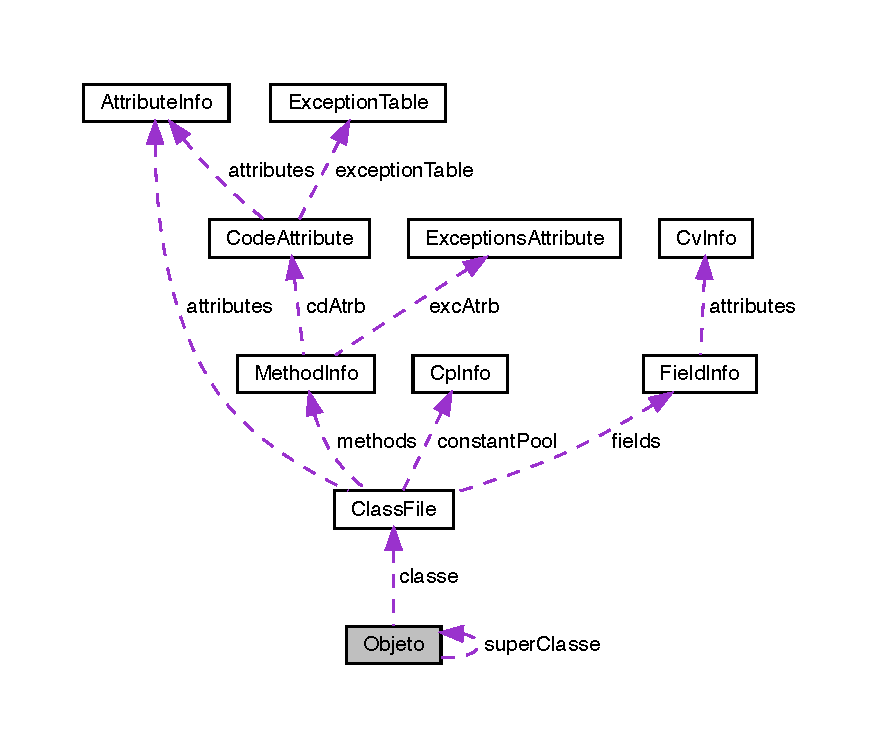
\includegraphics[width=350pt]{structObjeto__coll__graph}
\end{center}
\end{figure}
\subsection*{Public Attributes}
\begin{DoxyCompactItemize}
\item 
\mbox{\Hypertarget{structObjeto_a5596a470c07ffff562f21911fc34fbf3}\label{structObjeto_a5596a470c07ffff562f21911fc34fbf3}} 
\mbox{\hyperlink{structClassFile}{Class\+File}} $\ast$ {\bfseries classe}
\item 
\mbox{\Hypertarget{structObjeto_aa7b097e2dea86e221a2c7fc1c85b6fe5}\label{structObjeto_aa7b097e2dea86e221a2c7fc1c85b6fe5}} 
struct \mbox{\hyperlink{structObjeto}{Objeto}} $\ast$ {\bfseries super\+Classe}
\item 
\mbox{\Hypertarget{structObjeto_a744a42e5e611e1d2d2f65842f4117f7b}\label{structObjeto_a744a42e5e611e1d2d2f65842f4117f7b}} 
uint32\+\_\+t $\ast$ {\bfseries campos}
\item 
\mbox{\Hypertarget{structObjeto_a7561a3d822608137d47d2babf2dd9048}\label{structObjeto_a7561a3d822608137d47d2babf2dd9048}} 
uint32\+\_\+t $\ast$ {\bfseries indice\+Campos}
\end{DoxyCompactItemize}


\subsection{Detailed Description}
Estrutura para um objeto java. 

Essa estrutura guarda todas as informacoes especificas de cada objeto instanciado. 

The documentation for this struct was generated from the following file\+:\begin{DoxyCompactItemize}
\item 
\mbox{\hyperlink{areaMetodos_8h}{area\+Metodos.\+h}}\end{DoxyCompactItemize}

\hypertarget{structPilhaOp}{}\section{Pilha\+Op Struct Reference}
\label{structPilhaOp}\index{Pilha\+Op@{Pilha\+Op}}
\subsection*{Public Attributes}
\begin{DoxyCompactItemize}
\item 
\mbox{\Hypertarget{structPilhaOp_ad3fdbfc30e2a1b62169ce905a3af6a39}\label{structPilhaOp_ad3fdbfc30e2a1b62169ce905a3af6a39}} 
int {\bfseries depth}
\item 
\mbox{\Hypertarget{structPilhaOp_a66868e47a39d4f335823ae7de24947bf}\label{structPilhaOp_a66868e47a39d4f335823ae7de24947bf}} 
int32\+\_\+t $\ast$ {\bfseries operandos}
\end{DoxyCompactItemize}


The documentation for this struct was generated from the following file\+:\begin{DoxyCompactItemize}
\item 
\hyperlink{frame_8h}{frame.\+h}\end{DoxyCompactItemize}

\hypertarget{structStackFrame}{}\section{Stack\+Frame Struct Reference}
\label{structStackFrame}\index{StackFrame@{StackFrame}}


Collaboration diagram for Stack\+Frame\+:
\nopagebreak
\begin{figure}[H]
\begin{center}
\leavevmode
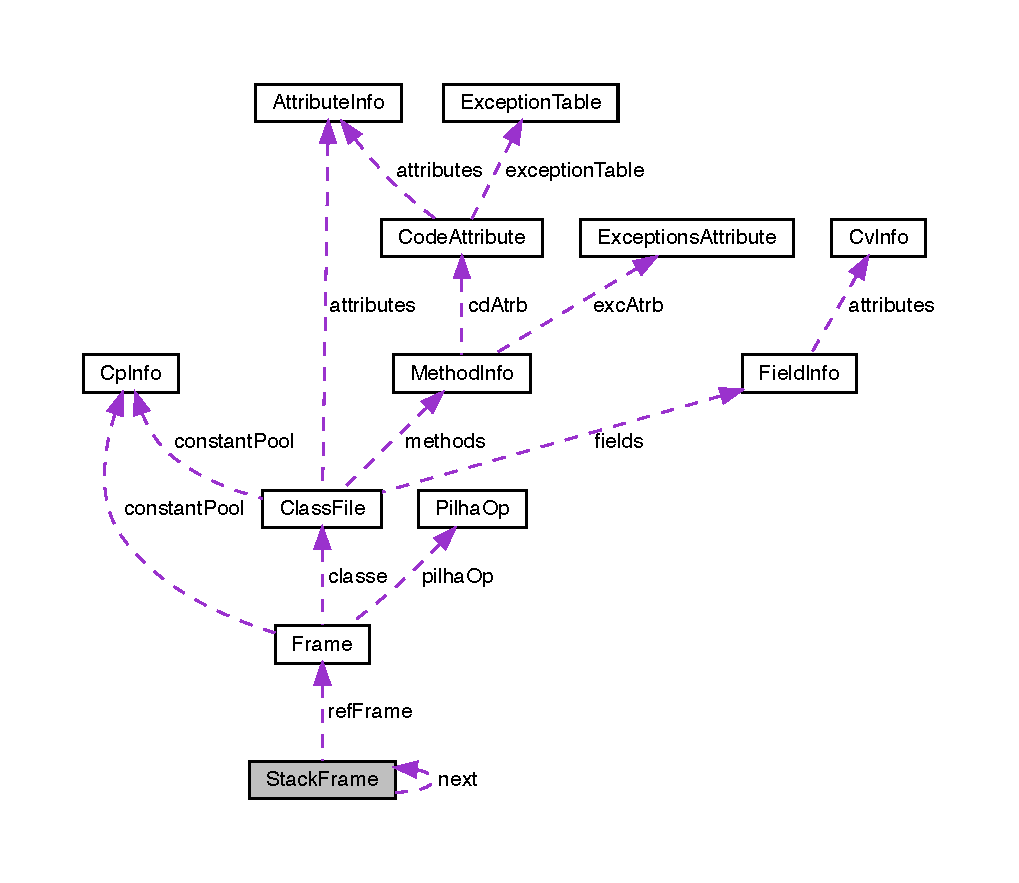
\includegraphics[width=350pt]{structStackFrame__coll__graph}
\end{center}
\end{figure}
\subsection*{Public Attributes}
\begin{DoxyCompactItemize}
\item 
\mbox{\Hypertarget{structStackFrame_aee414b80c97dcb5e37632a64bbcbff1c}\label{structStackFrame_aee414b80c97dcb5e37632a64bbcbff1c}} 
\mbox{\hyperlink{structFrame}{Frame}} $\ast$ {\bfseries ref\+Frame}
\item 
\mbox{\Hypertarget{structStackFrame_a3cb6ca230d221991df6c9f554aa7a43b}\label{structStackFrame_a3cb6ca230d221991df6c9f554aa7a43b}} 
struct \mbox{\hyperlink{structStackFrame}{Stack\+Frame}} $\ast$ {\bfseries next}
\end{DoxyCompactItemize}


The documentation for this struct was generated from the following file\+:\begin{DoxyCompactItemize}
\item 
\mbox{\hyperlink{frame_8h}{frame.\+h}}\end{DoxyCompactItemize}

\hypertarget{structVector}{}\section{Vector Struct Reference}
\label{structVector}\index{Vector@{Vector}}
\subsection*{Public Attributes}
\begin{DoxyCompactItemize}
\item 
\mbox{\Hypertarget{structVector_a0f2af0912b4d39a569c01fc73c409b0f}\label{structVector_a0f2af0912b4d39a569c01fc73c409b0f}} 
int32\+\_\+t {\bfseries referencia}
\item 
\mbox{\Hypertarget{structVector_a7444f49069adbd72108bda57a0585476}\label{structVector_a7444f49069adbd72108bda57a0585476}} 
int32\+\_\+t {\bfseries tamanho}
\item 
\mbox{\Hypertarget{structVector_a7dfc8127c1b5681c6b4ccd3c036710e7}\label{structVector_a7dfc8127c1b5681c6b4ccd3c036710e7}} 
int8\+\_\+t {\bfseries tipo}
\end{DoxyCompactItemize}


The documentation for this struct was generated from the following file\+:\begin{DoxyCompactItemize}
\item 
\mbox{\hyperlink{frame_8h}{frame.\+h}}\end{DoxyCompactItemize}

\chapter{File Documentation}
\hypertarget{areaMetodos_8h}{}\section{area\+Metodos.\+h File Reference}
\label{areaMetodos_8h}\index{areaMetodos.h@{areaMetodos.h}}


Define as estruturas Area de Metodos e \mbox{\hyperlink{structObjeto}{Objeto}}.  


{\ttfamily \#include \char`\"{}leitor.\+h\char`\"{}}\newline
Include dependency graph for area\+Metodos.\+h\+:
\nopagebreak
\begin{figure}[H]
\begin{center}
\leavevmode
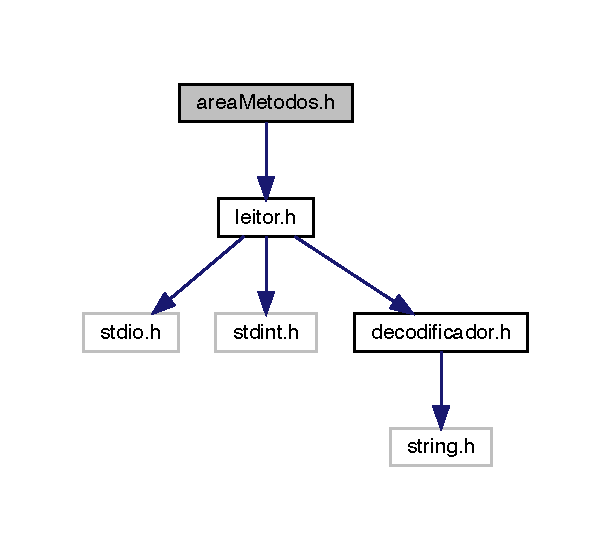
\includegraphics[width=293pt]{areaMetodos_8h__incl}
\end{center}
\end{figure}
This graph shows which files directly or indirectly include this file\+:
\nopagebreak
\begin{figure}[H]
\begin{center}
\leavevmode
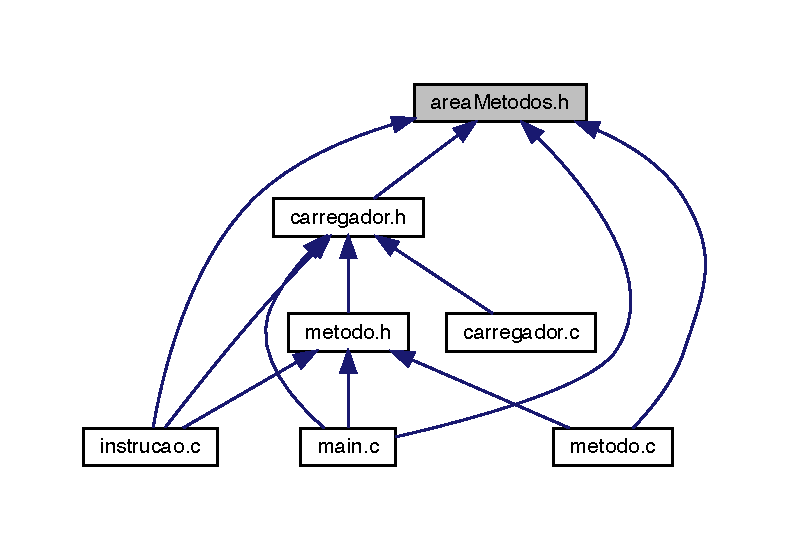
\includegraphics[width=350pt]{areaMetodos_8h__dep__incl}
\end{center}
\end{figure}
\subsection*{Classes}
\begin{DoxyCompactItemize}
\item 
struct \mbox{\hyperlink{structAreaMetodos}{Area\+Metodos}}
\begin{DoxyCompactList}\small\item\em Estrutura geral que contem todas as demais estruturas. \end{DoxyCompactList}\item 
struct \mbox{\hyperlink{structObjeto}{Objeto}}
\begin{DoxyCompactList}\small\item\em Estrutura para um objeto java. \end{DoxyCompactList}\end{DoxyCompactItemize}
\subsection*{Typedefs}
\begin{DoxyCompactItemize}
\item 
typedef struct \mbox{\hyperlink{structAreaMetodos}{Area\+Metodos}} \mbox{\hyperlink{areaMetodos_8h_a61a43b36ea956f6d27a33c4a8150aa42}{Area\+Metodos}}
\begin{DoxyCompactList}\small\item\em Estrutura geral que contem todas as demais estruturas. \end{DoxyCompactList}\item 
typedef struct \mbox{\hyperlink{structObjeto}{Objeto}} \mbox{\hyperlink{areaMetodos_8h_af86b4905bd1a5f5fbbc9be8105708e0f}{Objeto}}
\begin{DoxyCompactList}\small\item\em Estrutura para um objeto java. \end{DoxyCompactList}\end{DoxyCompactItemize}


\subsection{Detailed Description}
Define as estruturas Area de Metodos e \mbox{\hyperlink{structObjeto}{Objeto}}. 

\begin{DoxyDate}{Date}
28/06/2019.
\end{DoxyDate}
\begin{DoxyAuthor}{Authors}
Bruno Sanguinetti 18/0046063 ~\newline
Gabriel Vasconcelos 16/0120781 ~\newline
Leonardo de Almeida 15/0135491 ~\newline
Lucas Mafra 12/0126443 ~\newline
Wladimir Gramacho 15/0058718 ~\newline

\end{DoxyAuthor}


\subsection{Typedef Documentation}
\mbox{\Hypertarget{areaMetodos_8h_a61a43b36ea956f6d27a33c4a8150aa42}\label{areaMetodos_8h_a61a43b36ea956f6d27a33c4a8150aa42}} 
\index{areaMetodos.h@{areaMetodos.h}!AreaMetodos@{AreaMetodos}}
\index{AreaMetodos@{AreaMetodos}!areaMetodos.h@{areaMetodos.h}}
\subsubsection{\texorpdfstring{AreaMetodos}{AreaMetodos}}
{\footnotesize\ttfamily typedef struct \mbox{\hyperlink{structAreaMetodos}{Area\+Metodos}}  \mbox{\hyperlink{structAreaMetodos}{Area\+Metodos}}}



Estrutura geral que contem todas as demais estruturas. 

Aqui ficam guaradas as classes carregadas e todas as subestrutures dessas classes. \mbox{\Hypertarget{areaMetodos_8h_af86b4905bd1a5f5fbbc9be8105708e0f}\label{areaMetodos_8h_af86b4905bd1a5f5fbbc9be8105708e0f}} 
\index{areaMetodos.h@{areaMetodos.h}!Objeto@{Objeto}}
\index{Objeto@{Objeto}!areaMetodos.h@{areaMetodos.h}}
\subsubsection{\texorpdfstring{Objeto}{Objeto}}
{\footnotesize\ttfamily typedef struct \mbox{\hyperlink{structObjeto}{Objeto}}  \mbox{\hyperlink{structObjeto}{Objeto}}}



Estrutura para um objeto java. 

Essa estrutura guarda todas as informacoes especificas de cada objeto instanciado. 
\hypertarget{carregador_8c}{}\section{carregador.\+c File Reference}
\label{carregador_8c}\index{carregador.\+c@{carregador.\+c}}


Carrega, inicializa e aloca um \hyperlink{structClassFile}{Class\+File} e associa com a estrutura do \hyperlink{structAreaMetodos}{Area\+Metodos}.  


{\ttfamily \#include \char`\"{}carregador.\+h\char`\"{}}\newline
{\ttfamily \#include $<$string.\+h$>$}\newline
{\ttfamily \#include $<$stdio.\+h$>$}\newline
{\ttfamily \#include $<$stdlib.\+h$>$}\newline
Include dependency graph for carregador.\+c\+:
% FIG 0
\subsection*{Macros}
\begin{DoxyCompactItemize}
\item 
\mbox{\Hypertarget{carregador_8c_aa93f0eb578d23995850d61f7d61c55c1}\label{carregador_8c_aa93f0eb578d23995850d61f7d61c55c1}} 
\#define {\bfseries F\+A\+L\+SE}~0
\item 
\mbox{\Hypertarget{carregador_8c_aa8cecfc5c5c054d2875c03e77b7be15d}\label{carregador_8c_aa8cecfc5c5c054d2875c03e77b7be15d}} 
\#define {\bfseries T\+R\+UE}~1
\end{DoxyCompactItemize}
\subsection*{Functions}
\begin{DoxyCompactItemize}
\item 
void \hyperlink{carregador_8c_a63bb151e862226cbf006d6b1fa345b8b}{valida\+Nome\+Classe\+Arquivo} (\hyperlink{structClassFile}{Class\+File} $\ast$class\+File\+Lido, char $\ast$caminho\+Classe)
\item 
void \hyperlink{carregador_8c_ae550e684ba0b0a11753fd24e1512f7be}{valida\+Versao\+Java} (\hyperlink{structClassFile}{Class\+File} $\ast$class\+File\+Lido)
\item 
void \hyperlink{carregador_8c_a0010614c11b7e7a4bd8aad07ce816546}{valida\+Class\+File} (\hyperlink{structClassFile}{Class\+File} $\ast$class\+File\+Lido, char $\ast$caminho\+Classe)
\item 
int32\+\_\+t \hyperlink{carregador_8c_aa8226828a719a729baa6de54497dbd06}{carrega\+Classe\+Para\+Memoria} (char $\ast$caminho\+Classe)
\item 
void \hyperlink{carregador_8c_ad79fe3f83657a5542b2278537ccfbdd1}{inicializa\+Primeira\+Vez} ()
\item 
char $\ast$ \hyperlink{carregador_8c_a9c9a3135d3a02d275706a00116816824}{retorna\+Nome\+Class} (\hyperlink{structClassFile}{Class\+File} $\ast$classe)
\item 
\hyperlink{structClassFile}{Class\+File} $\ast$ \hyperlink{carregador_8c_a5791c228ebcf57d6eb24ba9618eae973}{busca\+Class\+Por\+Indice} (int indice)
\item 
char $\ast$ \hyperlink{carregador_8c_aac550604e02bb2506492757b974c6856}{retorna\+Nome} (\hyperlink{structClassFile}{Class\+File} $\ast$classe, uint16\+\_\+t indice\+Nome)
\end{DoxyCompactItemize}
\subsection*{Variables}
\begin{DoxyCompactItemize}
\item 
\mbox{\Hypertarget{carregador_8c_ac2492b2ee633ac35c62b2632b337c557}\label{carregador_8c_ac2492b2ee633ac35c62b2632b337c557}} 
\hyperlink{structAreaMetodos}{Area\+Metodos} {\bfseries area\+Metodos}
\item 
\mbox{\Hypertarget{carregador_8c_a5b93f1b26aba4ad5cbecbf642d6f9944}\label{carregador_8c_a5b93f1b26aba4ad5cbecbf642d6f9944}} 
int {\bfseries primeira} = F\+A\+L\+SE
\end{DoxyCompactItemize}


\subsection{Detailed Description}
Carrega, inicializa e aloca um \hyperlink{structClassFile}{Class\+File} e associa com a estrutura do \hyperlink{structAreaMetodos}{Area\+Metodos}. 

\begin{DoxyAuthor}{Authors}
Bruno Sanguinetti 18/0046063 ~\newline
Gabriel Vasconcelos 16/0120781 ~\newline
Leonardo de Almeida 15/0135491 ~\newline
Lucas Mafra 12/0126443 ~\newline
Wladimir Gramacho 15/0058718 ~\newline
 
\end{DoxyAuthor}
\begin{DoxyDate}{Date}
28/06/2019 
\end{DoxyDate}


\subsection{Function Documentation}
\mbox{\Hypertarget{carregador_8c_a5791c228ebcf57d6eb24ba9618eae973}\label{carregador_8c_a5791c228ebcf57d6eb24ba9618eae973}} 
\index{carregador.\+c@{carregador.\+c}!busca\+Class\+Por\+Indice@{busca\+Class\+Por\+Indice}}
\index{busca\+Class\+Por\+Indice@{busca\+Class\+Por\+Indice}!carregador.\+c@{carregador.\+c}}
\subsubsection{\texorpdfstring{busca\+Class\+Por\+Indice()}{buscaClassPorIndice()}}
{\footnotesize\ttfamily \hyperlink{structClassFile}{Class\+File}$\ast$ busca\+Class\+Por\+Indice (\begin{DoxyParamCaption}\item[{int}]{indice }\end{DoxyParamCaption})}

Caso o indice passado seja um numero menor que o numero de classes salvas na area de metodos.


\begin{DoxyParams}{Parameters}
{\em int} & Indice da classe no array de area de metodos que se deseja saber. \\
\hline
\end{DoxyParams}
\begin{DoxyReturn}{Returns}
{\ttfamily Class\+File$\ast$} retorna um ponteiro para a classe apontada por esse indice no array da area de metodos. 
\end{DoxyReturn}
\mbox{\Hypertarget{carregador_8c_aa8226828a719a729baa6de54497dbd06}\label{carregador_8c_aa8226828a719a729baa6de54497dbd06}} 
\index{carregador.\+c@{carregador.\+c}!carrega\+Classe\+Para\+Memoria@{carrega\+Classe\+Para\+Memoria}}
\index{carrega\+Classe\+Para\+Memoria@{carrega\+Classe\+Para\+Memoria}!carregador.\+c@{carregador.\+c}}
\subsubsection{\texorpdfstring{carrega\+Classe\+Para\+Memoria()}{carregaClasseParaMemoria()}}
{\footnotesize\ttfamily int32\+\_\+t carrega\+Classe\+Para\+Memoria (\begin{DoxyParamCaption}\item[{char $\ast$}]{caminho\+Classe }\end{DoxyParamCaption})}

Carrega o arquivo .class na memoria e adiciona a classe na area de metodos.


\begin{DoxyParams}{Parameters}
{\em char$\ast$} & Contem o caminho para a classe a ser lida. \\
\hline
\end{DoxyParams}
\begin{DoxyReturn}{Returns}
{\ttfamily int32\+\_\+t} Retorna o numero de classes em area de metodos -\/ 1 
\end{DoxyReturn}
\begin{DoxySeeAlso}{See also}
\hyperlink{carregador_8c_ad79fe3f83657a5542b2278537ccfbdd1}{inicializa\+Primeira\+Vez} \hyperlink{leitor_8h_a658f67ed6a3ca72248e7cc0eaba67ba5}{inicializa\+Leitor} 
\end{DoxySeeAlso}
\mbox{\Hypertarget{carregador_8c_ad79fe3f83657a5542b2278537ccfbdd1}\label{carregador_8c_ad79fe3f83657a5542b2278537ccfbdd1}} 
\index{carregador.\+c@{carregador.\+c}!inicializa\+Primeira\+Vez@{inicializa\+Primeira\+Vez}}
\index{inicializa\+Primeira\+Vez@{inicializa\+Primeira\+Vez}!carregador.\+c@{carregador.\+c}}
\subsubsection{\texorpdfstring{inicializa\+Primeira\+Vez()}{inicializaPrimeiraVez()}}
{\footnotesize\ttfamily void inicializa\+Primeira\+Vez (\begin{DoxyParamCaption}{ }\end{DoxyParamCaption})}

Incializa o valor de area\+Metodos.\+num\+Classes com 0 caso seja a primeira classe a ser lida. Seta uma variavel global para indicar que a primeira classe ja foi lida.


\begin{DoxyParams}{Parameters}
{\em Nao} & possui parametros \\
\hline
\end{DoxyParams}
\begin{DoxyReturn}{Returns}
{\ttfamily void} 
\end{DoxyReturn}
\mbox{\Hypertarget{carregador_8c_aac550604e02bb2506492757b974c6856}\label{carregador_8c_aac550604e02bb2506492757b974c6856}} 
\index{carregador.\+c@{carregador.\+c}!retorna\+Nome@{retorna\+Nome}}
\index{retorna\+Nome@{retorna\+Nome}!carregador.\+c@{carregador.\+c}}
\subsubsection{\texorpdfstring{retorna\+Nome()}{retornaNome()}}
{\footnotesize\ttfamily char$\ast$ retorna\+Nome (\begin{DoxyParamCaption}\item[{\hyperlink{structClassFile}{Class\+File} $\ast$}]{classe,  }\item[{uint16\+\_\+t}]{indice\+Nome }\end{DoxyParamCaption})}

Retorna o nome da classe desejada com base no classfile e no indice do nome.


\begin{DoxyParams}{Parameters}
{\em Class\+File$\ast$} & Classe que se deseja saber o nome. \\
\hline
{\em uint16\+\_\+t} & Indce da classe. \\
\hline
\end{DoxyParams}
\begin{DoxyReturn}{Returns}
{\ttfamily char$\ast$} Retorna o nome da classe desejada com base no classfile e no indice do nome. 
\end{DoxyReturn}
\mbox{\Hypertarget{carregador_8c_a9c9a3135d3a02d275706a00116816824}\label{carregador_8c_a9c9a3135d3a02d275706a00116816824}} 
\index{carregador.\+c@{carregador.\+c}!retorna\+Nome\+Class@{retorna\+Nome\+Class}}
\index{retorna\+Nome\+Class@{retorna\+Nome\+Class}!carregador.\+c@{carregador.\+c}}
\subsubsection{\texorpdfstring{retorna\+Nome\+Class()}{retornaNomeClass()}}
{\footnotesize\ttfamily char$\ast$ retorna\+Nome\+Class (\begin{DoxyParamCaption}\item[{\hyperlink{structClassFile}{Class\+File} $\ast$}]{classe }\end{DoxyParamCaption})}

Retorna o nome da classe desejada.


\begin{DoxyParams}{Parameters}
{\em Class\+File$\ast$} & Classe que se deseja saber o nome. \\
\hline
\end{DoxyParams}
\begin{DoxyReturn}{Returns}
{\ttfamily char$\ast$} Nome da classe desejada 
\end{DoxyReturn}
\mbox{\Hypertarget{carregador_8c_a0010614c11b7e7a4bd8aad07ce816546}\label{carregador_8c_a0010614c11b7e7a4bd8aad07ce816546}} 
\index{carregador.\+c@{carregador.\+c}!valida\+Class\+File@{valida\+Class\+File}}
\index{valida\+Class\+File@{valida\+Class\+File}!carregador.\+c@{carregador.\+c}}
\subsubsection{\texorpdfstring{valida\+Class\+File()}{validaClassFile()}}
{\footnotesize\ttfamily void valida\+Class\+File (\begin{DoxyParamCaption}\item[{\hyperlink{structClassFile}{Class\+File} $\ast$}]{class\+File\+Lido,  }\item[{char $\ast$}]{caminho\+Classe }\end{DoxyParamCaption})}

Funcao que verifica se o .class carregado e ou nao a classe Object Se for, skipa validacao, se nao, valida chama as funcoes que validam consistencia da versao do Java e nome da classe no arquivo 
\begin{DoxyParams}{Parameters}
{\em Class\+File$\ast$} & contendo o .class lido \\
\hline
{\em char$\ast$} & contendo o nome do arquivo .class \\
\hline
\end{DoxyParams}
\begin{DoxyReturn}{Returns}
void 
\end{DoxyReturn}
\mbox{\Hypertarget{carregador_8c_a63bb151e862226cbf006d6b1fa345b8b}\label{carregador_8c_a63bb151e862226cbf006d6b1fa345b8b}} 
\index{carregador.\+c@{carregador.\+c}!valida\+Nome\+Classe\+Arquivo@{valida\+Nome\+Classe\+Arquivo}}
\index{valida\+Nome\+Classe\+Arquivo@{valida\+Nome\+Classe\+Arquivo}!carregador.\+c@{carregador.\+c}}
\subsubsection{\texorpdfstring{valida\+Nome\+Classe\+Arquivo()}{validaNomeClasseArquivo()}}
{\footnotesize\ttfamily void valida\+Nome\+Classe\+Arquivo (\begin{DoxyParamCaption}\item[{\hyperlink{structClassFile}{Class\+File} $\ast$}]{class\+File\+Lido,  }\item[{char $\ast$}]{caminho\+Classe }\end{DoxyParamCaption})}

Valida o nome do arquivo e o nome da classe. A execucao da J\+VM so deve continuar se forem iguais.


\begin{DoxyParams}{Parameters}
{\em Class\+File$\ast$} & contendo o .class lido \\
\hline
{\em char$\ast$} & contendo o nome do arquivo .class \\
\hline
\end{DoxyParams}
\begin{DoxyReturn}{Returns}
void 
\end{DoxyReturn}
\mbox{\Hypertarget{carregador_8c_ae550e684ba0b0a11753fd24e1512f7be}\label{carregador_8c_ae550e684ba0b0a11753fd24e1512f7be}} 
\index{carregador.\+c@{carregador.\+c}!valida\+Versao\+Java@{valida\+Versao\+Java}}
\index{valida\+Versao\+Java@{valida\+Versao\+Java}!carregador.\+c@{carregador.\+c}}
\subsubsection{\texorpdfstring{valida\+Versao\+Java()}{validaVersaoJava()}}
{\footnotesize\ttfamily void valida\+Versao\+Java (\begin{DoxyParamCaption}\item[{\hyperlink{structClassFile}{Class\+File} $\ast$}]{class\+File\+Lido }\end{DoxyParamCaption})}

Valida a versao do java lido no arquivo .class Essa implementacao da J\+VM so suporta ate Java 8 
\begin{DoxyParams}{Parameters}
{\em Class\+File$\ast$} & contendo o nome do arquivo .class \\
\hline
\end{DoxyParams}
\begin{DoxyReturn}{Returns}
void 
\end{DoxyReturn}

\hypertarget{carregador_8h}{}\section{carregador.\+h File Reference}
\label{carregador_8h}\index{carregador.h@{carregador.h}}
{\ttfamily \#include \char`\"{}leitor.\+h\char`\"{}}\newline
{\ttfamily \#include \char`\"{}area\+Metodos.\+h\char`\"{}}\newline
Include dependency graph for carregador.\+h\+:
\nopagebreak
\begin{figure}[H]
\begin{center}
\leavevmode
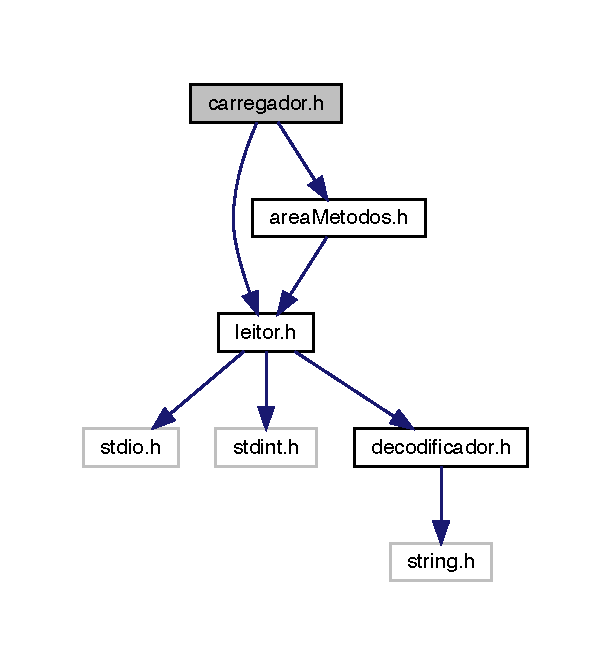
\includegraphics[width=293pt]{carregador_8h__incl}
\end{center}
\end{figure}
This graph shows which files directly or indirectly include this file\+:
\nopagebreak
\begin{figure}[H]
\begin{center}
\leavevmode
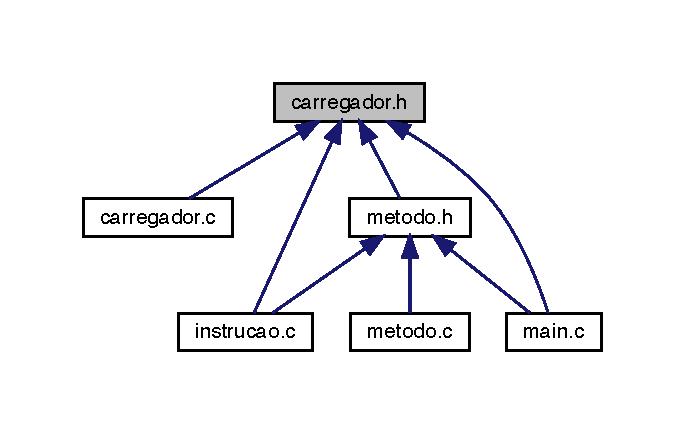
\includegraphics[width=329pt]{carregador_8h__dep__incl}
\end{center}
\end{figure}
\subsection*{Functions}
\begin{DoxyCompactItemize}
\item 
int32\+\_\+t \mbox{\hyperlink{carregador_8h_a6be3551b88a5154690e9e147217ca181}{carrega\+Classe\+Para\+Memoria}} (char $\ast$)
\item 
void \mbox{\hyperlink{carregador_8h_ad79fe3f83657a5542b2278537ccfbdd1}{inicializa\+Primeira\+Vez}} ()
\item 
\mbox{\Hypertarget{carregador_8h_ae145a82d8836f492083cb0151f5cbd9f}\label{carregador_8h_ae145a82d8836f492083cb0151f5cbd9f}} 
void {\bfseries carrega\+Classe} (char $\ast$)
\item 
char $\ast$ \mbox{\hyperlink{carregador_8h_aabea5c0cd0e77aed6f86127bd403918c}{retorna\+Nome\+Class}} (\mbox{\hyperlink{structClassFile}{Class\+File}} $\ast$)
\item 
\mbox{\hyperlink{structClassFile}{Class\+File}} $\ast$ \mbox{\hyperlink{carregador_8h_a5e44435bd5cfcea055179495059b1b2d}{busca\+Class\+Por\+Indice}} (int)
\item 
char $\ast$ \mbox{\hyperlink{carregador_8h_af24376339440bd0224ad335b9b4cbef6}{retorna\+Nome}} (\mbox{\hyperlink{structClassFile}{Class\+File}} $\ast$, uint16\+\_\+t)
\item 
void \mbox{\hyperlink{carregador_8h_a55c6dbf46daeac1e1bd59b648a5da4df}{valida\+Class\+File}} (\mbox{\hyperlink{structClassFile}{Class\+File}} $\ast$, char $\ast$)
\item 
void \mbox{\hyperlink{carregador_8h_a0afba62d7dd523b5f93a206be25465b4}{valida\+Versao\+Java}} (\mbox{\hyperlink{structClassFile}{Class\+File}} $\ast$)
\item 
void \mbox{\hyperlink{carregador_8h_a7a0b164d89fdb873d205a7f689b645dc}{valida\+Nome\+Classe\+Arquivo}} (\mbox{\hyperlink{structClassFile}{Class\+File}} $\ast$, char $\ast$)
\end{DoxyCompactItemize}


\subsection{Function Documentation}
\mbox{\Hypertarget{carregador_8h_a5e44435bd5cfcea055179495059b1b2d}\label{carregador_8h_a5e44435bd5cfcea055179495059b1b2d}} 
\index{carregador.h@{carregador.h}!buscaClassPorIndice@{buscaClassPorIndice}}
\index{buscaClassPorIndice@{buscaClassPorIndice}!carregador.h@{carregador.h}}
\subsubsection{\texorpdfstring{buscaClassPorIndice()}{buscaClassPorIndice()}}
{\footnotesize\ttfamily \mbox{\hyperlink{structClassFile}{Class\+File}}$\ast$ busca\+Class\+Por\+Indice (\begin{DoxyParamCaption}\item[{int}]{indice }\end{DoxyParamCaption})}

Caso o indice passado seja um numero menor que o numero de classes salvas na area de metodos.


\begin{DoxyParams}{Parameters}
{\em int} & Indice da classe no array de area de metodos que se deseja saber. \\
\hline
\end{DoxyParams}
\begin{DoxyReturn}{Returns}
{\ttfamily Class\+File$\ast$} retorna um ponteiro para a classe apontada por esse indice no array da area de metodos. 
\end{DoxyReturn}
\mbox{\Hypertarget{carregador_8h_a6be3551b88a5154690e9e147217ca181}\label{carregador_8h_a6be3551b88a5154690e9e147217ca181}} 
\index{carregador.h@{carregador.h}!carregaClasseParaMemoria@{carregaClasseParaMemoria}}
\index{carregaClasseParaMemoria@{carregaClasseParaMemoria}!carregador.h@{carregador.h}}
\subsubsection{\texorpdfstring{carregaClasseParaMemoria()}{carregaClasseParaMemoria()}}
{\footnotesize\ttfamily int32\+\_\+t carrega\+Classe\+Para\+Memoria (\begin{DoxyParamCaption}\item[{char $\ast$}]{caminho\+Classe }\end{DoxyParamCaption})}

Carrega o arquivo .class na memoria e adiciona a classe na area de metodos.


\begin{DoxyParams}{Parameters}
{\em char$\ast$} & Contem o caminho para a classe a ser lida. \\
\hline
\end{DoxyParams}
\begin{DoxyReturn}{Returns}
{\ttfamily int32\+\_\+t} Retorna o numero de classes em area de metodos -\/ 1 
\end{DoxyReturn}
\begin{DoxySeeAlso}{See also}
\mbox{\hyperlink{carregador_8c_ad79fe3f83657a5542b2278537ccfbdd1}{inicializa\+Primeira\+Vez}} \mbox{\hyperlink{leitor_8h_a658f67ed6a3ca72248e7cc0eaba67ba5}{inicializa\+Leitor}} 
\end{DoxySeeAlso}
\mbox{\Hypertarget{carregador_8h_ad79fe3f83657a5542b2278537ccfbdd1}\label{carregador_8h_ad79fe3f83657a5542b2278537ccfbdd1}} 
\index{carregador.h@{carregador.h}!inicializaPrimeiraVez@{inicializaPrimeiraVez}}
\index{inicializaPrimeiraVez@{inicializaPrimeiraVez}!carregador.h@{carregador.h}}
\subsubsection{\texorpdfstring{inicializaPrimeiraVez()}{inicializaPrimeiraVez()}}
{\footnotesize\ttfamily void inicializa\+Primeira\+Vez (\begin{DoxyParamCaption}{ }\end{DoxyParamCaption})}

Incializa o valor de area\+Metodos.\+num\+Classes com 0 caso seja a primeira classe a ser lida. Seta uma variavel global para indicar que a primeira classe ja foi lida.


\begin{DoxyParams}{Parameters}
{\em Nao} & possui parametros \\
\hline
\end{DoxyParams}
\begin{DoxyReturn}{Returns}
{\ttfamily void} 
\end{DoxyReturn}
\mbox{\Hypertarget{carregador_8h_af24376339440bd0224ad335b9b4cbef6}\label{carregador_8h_af24376339440bd0224ad335b9b4cbef6}} 
\index{carregador.h@{carregador.h}!retornaNome@{retornaNome}}
\index{retornaNome@{retornaNome}!carregador.h@{carregador.h}}
\subsubsection{\texorpdfstring{retornaNome()}{retornaNome()}}
{\footnotesize\ttfamily char$\ast$ retorna\+Nome (\begin{DoxyParamCaption}\item[{\mbox{\hyperlink{structClassFile}{Class\+File}} $\ast$}]{classe,  }\item[{uint16\+\_\+t}]{indice\+Nome }\end{DoxyParamCaption})}

Retorna o nome da classe desejada com base no classfile e no indice do nome.


\begin{DoxyParams}{Parameters}
{\em Class\+File$\ast$} & Classe que se deseja saber o nome. \\
\hline
{\em uint16\+\_\+t} & Indce da classe. \\
\hline
\end{DoxyParams}
\begin{DoxyReturn}{Returns}
{\ttfamily char$\ast$} Retorna o nome da classe desejada com base no classfile e no indice do nome. 
\end{DoxyReturn}
\mbox{\Hypertarget{carregador_8h_aabea5c0cd0e77aed6f86127bd403918c}\label{carregador_8h_aabea5c0cd0e77aed6f86127bd403918c}} 
\index{carregador.h@{carregador.h}!retornaNomeClass@{retornaNomeClass}}
\index{retornaNomeClass@{retornaNomeClass}!carregador.h@{carregador.h}}
\subsubsection{\texorpdfstring{retornaNomeClass()}{retornaNomeClass()}}
{\footnotesize\ttfamily char$\ast$ retorna\+Nome\+Class (\begin{DoxyParamCaption}\item[{\mbox{\hyperlink{structClassFile}{Class\+File}} $\ast$}]{classe }\end{DoxyParamCaption})}

Retorna o nome da classe desejada.


\begin{DoxyParams}{Parameters}
{\em Class\+File$\ast$} & Classe que se deseja saber o nome. \\
\hline
\end{DoxyParams}
\begin{DoxyReturn}{Returns}
{\ttfamily char$\ast$} Nome da classe desejada 
\end{DoxyReturn}
\mbox{\Hypertarget{carregador_8h_a55c6dbf46daeac1e1bd59b648a5da4df}\label{carregador_8h_a55c6dbf46daeac1e1bd59b648a5da4df}} 
\index{carregador.h@{carregador.h}!validaClassFile@{validaClassFile}}
\index{validaClassFile@{validaClassFile}!carregador.h@{carregador.h}}
\subsubsection{\texorpdfstring{validaClassFile()}{validaClassFile()}}
{\footnotesize\ttfamily void valida\+Class\+File (\begin{DoxyParamCaption}\item[{\mbox{\hyperlink{structClassFile}{Class\+File}} $\ast$}]{class\+File\+Lido,  }\item[{char $\ast$}]{caminho\+Classe }\end{DoxyParamCaption})}

Funcao que verifica se o .class carregado e ou nao a classe Object Se for, skipa validacao, se nao, valida chama as funcoes que validam consistencia da versao do Java e nome da classe no arquivo 
\begin{DoxyParams}{Parameters}
{\em Class\+File$\ast$} & contendo o .class lido \\
\hline
{\em char$\ast$} & contendo o nome do arquivo .class \\
\hline
\end{DoxyParams}
\begin{DoxyReturn}{Returns}
void 
\end{DoxyReturn}
\mbox{\Hypertarget{carregador_8h_a7a0b164d89fdb873d205a7f689b645dc}\label{carregador_8h_a7a0b164d89fdb873d205a7f689b645dc}} 
\index{carregador.h@{carregador.h}!validaNomeClasseArquivo@{validaNomeClasseArquivo}}
\index{validaNomeClasseArquivo@{validaNomeClasseArquivo}!carregador.h@{carregador.h}}
\subsubsection{\texorpdfstring{validaNomeClasseArquivo()}{validaNomeClasseArquivo()}}
{\footnotesize\ttfamily void valida\+Nome\+Classe\+Arquivo (\begin{DoxyParamCaption}\item[{\mbox{\hyperlink{structClassFile}{Class\+File}} $\ast$}]{class\+File\+Lido,  }\item[{char $\ast$}]{caminho\+Classe }\end{DoxyParamCaption})}

Valida o nome do arquivo e o nome da classe. A execucao da J\+VM so deve continuar se forem iguais.


\begin{DoxyParams}{Parameters}
{\em Class\+File$\ast$} & contendo o .class lido \\
\hline
{\em char$\ast$} & contendo o nome do arquivo .class \\
\hline
\end{DoxyParams}
\begin{DoxyReturn}{Returns}
void 
\end{DoxyReturn}
\mbox{\Hypertarget{carregador_8h_a0afba62d7dd523b5f93a206be25465b4}\label{carregador_8h_a0afba62d7dd523b5f93a206be25465b4}} 
\index{carregador.h@{carregador.h}!validaVersaoJava@{validaVersaoJava}}
\index{validaVersaoJava@{validaVersaoJava}!carregador.h@{carregador.h}}
\subsubsection{\texorpdfstring{validaVersaoJava()}{validaVersaoJava()}}
{\footnotesize\ttfamily void valida\+Versao\+Java (\begin{DoxyParamCaption}\item[{\mbox{\hyperlink{structClassFile}{Class\+File}} $\ast$}]{class\+File\+Lido }\end{DoxyParamCaption})}

Valida a versao do java lido no arquivo .class Essa implementacao da J\+VM so suporta ate Java 8 
\begin{DoxyParams}{Parameters}
{\em Class\+File$\ast$} & contendo o nome do arquivo .class \\
\hline
\end{DoxyParams}
\begin{DoxyReturn}{Returns}
void 
\end{DoxyReturn}

\hypertarget{decodificador_8c}{}\section{decodificador.\+c File Reference}
\label{decodificador_8c}\index{decodificador.c@{decodificador.c}}


Recebe uma estrutura \mbox{\hyperlink{structDecodificador}{Decodificador}} vazia e preenche com strings que sao as instrucoes presentes no bytecode. Retorna uma estrutura \mbox{\hyperlink{structDecodificador}{Decodificador}} preenchida.  


{\ttfamily \#include \char`\"{}decodificador.\+h\char`\"{}}\newline
Include dependency graph for decodificador.\+c\+:
\nopagebreak
\begin{figure}[H]
\begin{center}
\leavevmode
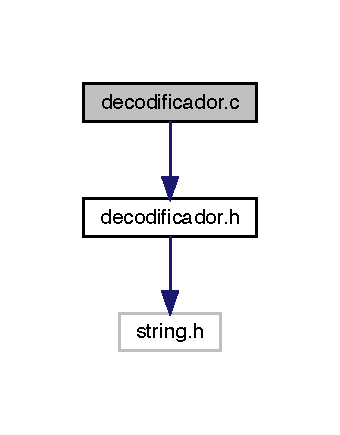
\includegraphics[width=163pt]{decodificador_8c__incl}
\end{center}
\end{figure}
\subsection*{Functions}
\begin{DoxyCompactItemize}
\item 
void \mbox{\hyperlink{decodificador_8c_ac4ac4bcce3fed96b1a2657ceafda40bc}{inicializa\+Decodificador}} (\mbox{\hyperlink{structDecodificador}{Decodificador}} decodificador\mbox{[}$\,$\mbox{]})
\end{DoxyCompactItemize}


\subsection{Detailed Description}
Recebe uma estrutura \mbox{\hyperlink{structDecodificador}{Decodificador}} vazia e preenche com strings que sao as instrucoes presentes no bytecode. Retorna uma estrutura \mbox{\hyperlink{structDecodificador}{Decodificador}} preenchida. 

\begin{DoxyAuthor}{Authors}
Bruno Sanguinetti 18/0046063 ~\newline
Gabriel Vasconcelos 16/0120781 ~\newline
Leonardo de Almeida 15/0135491 ~\newline
Lucas Mafra 12/0126443 ~\newline
Wladimir Gramacho 15/0058718 ~\newline
 
\end{DoxyAuthor}
\begin{DoxyDate}{Date}
11/07/2019 
\end{DoxyDate}


\subsection{Function Documentation}
\mbox{\Hypertarget{decodificador_8c_ac4ac4bcce3fed96b1a2657ceafda40bc}\label{decodificador_8c_ac4ac4bcce3fed96b1a2657ceafda40bc}} 
\index{decodificador.c@{decodificador.c}!inicializaDecodificador@{inicializaDecodificador}}
\index{inicializaDecodificador@{inicializaDecodificador}!decodificador.c@{decodificador.c}}
\subsubsection{\texorpdfstring{inicializaDecodificador()}{inicializaDecodificador()}}
{\footnotesize\ttfamily void inicializa\+Decodificador (\begin{DoxyParamCaption}\item[{\mbox{\hyperlink{structDecodificador}{Decodificador}}}]{decodificador\mbox{[}$\,$\mbox{]} }\end{DoxyParamCaption})}

Inicializa uma estrutura \mbox{\hyperlink{structDecodificador}{Decodificador}} com o nome das instrucoes e a quantidade de bytes que ela ocupa.


\begin{DoxyParams}{Parameters}
{\em \mbox{\hyperlink{structDecodificador}{Decodificador}}} & Um estrutura de \mbox{\hyperlink{structDecodificador}{Decodificador}} vazia \\
\hline
\end{DoxyParams}
\begin{DoxyReturn}{Returns}
{\ttfamily void} 
\end{DoxyReturn}

\hypertarget{decodificador_8h}{}\section{decodificador.\+h File Reference}
\label{decodificador_8h}\index{decodificador.h@{decodificador.h}}
{\ttfamily \#include $<$string.\+h$>$}\newline
Include dependency graph for decodificador.\+h\+:
\nopagebreak
\begin{figure}[H]
\begin{center}
\leavevmode
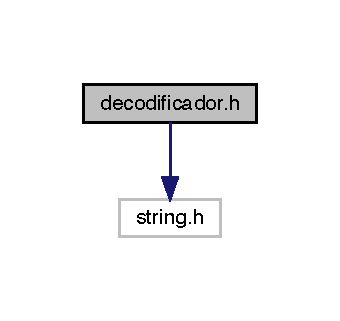
\includegraphics[width=163pt]{decodificador_8h__incl}
\end{center}
\end{figure}
This graph shows which files directly or indirectly include this file\+:
\nopagebreak
\begin{figure}[H]
\begin{center}
\leavevmode
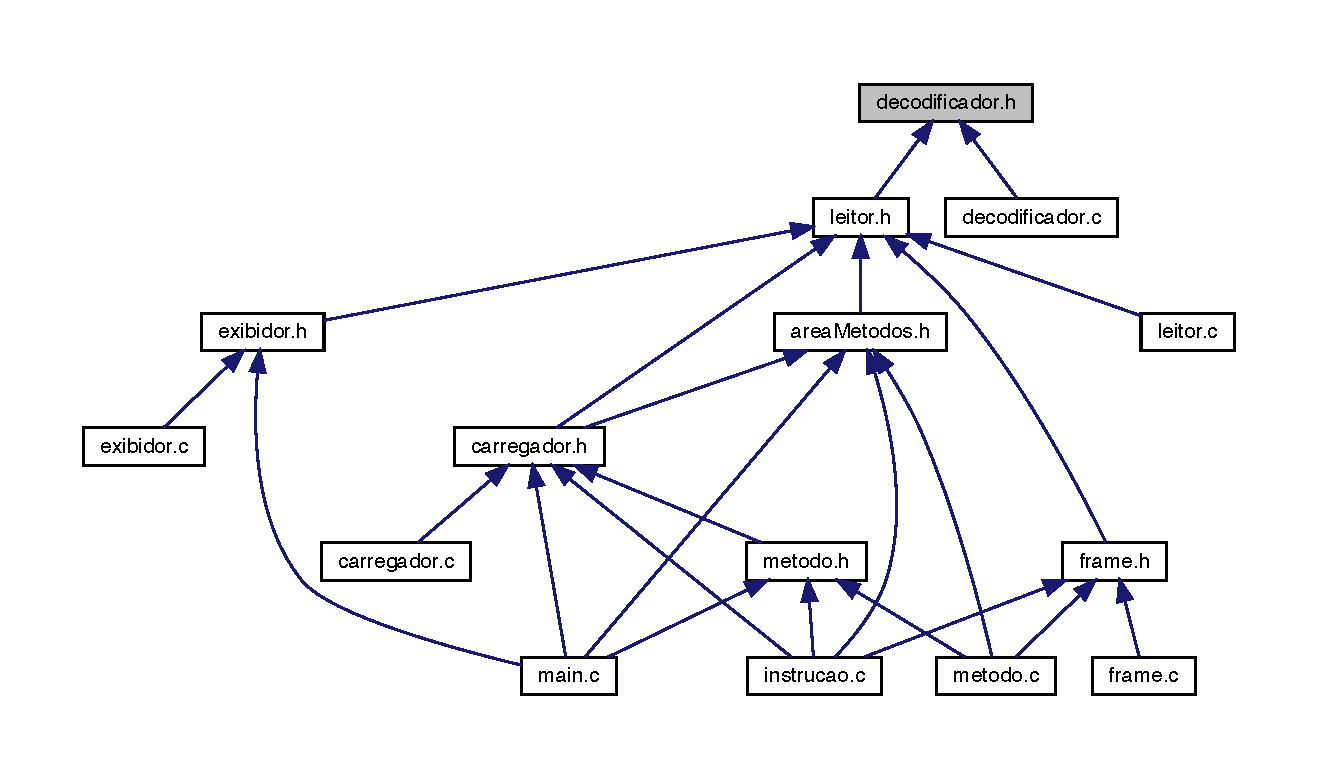
\includegraphics[width=350pt]{decodificador_8h__dep__incl}
\end{center}
\end{figure}
\subsection*{Classes}
\begin{DoxyCompactItemize}
\item 
struct \mbox{\hyperlink{structDecodificador}{Decodificador}}
\end{DoxyCompactItemize}
\subsection*{Macros}
\begin{DoxyCompactItemize}
\item 
\mbox{\Hypertarget{decodificador_8h_a33199dbdd3b5cb12a10b1cbd125293b8}\label{decodificador_8h_a33199dbdd3b5cb12a10b1cbd125293b8}} 
\#define {\bfseries N\+O\+M\+E\+\_\+\+I\+N\+S\+T\+R\+U\+C\+AO}~30
\end{DoxyCompactItemize}
\subsection*{Typedefs}
\begin{DoxyCompactItemize}
\item 
\mbox{\Hypertarget{decodificador_8h_af8f64bf402ebd05dd1314452e284031b}\label{decodificador_8h_af8f64bf402ebd05dd1314452e284031b}} 
typedef struct \mbox{\hyperlink{structDecodificador}{Decodificador}} {\bfseries Decodificador}
\end{DoxyCompactItemize}
\subsection*{Functions}
\begin{DoxyCompactItemize}
\item 
void \mbox{\hyperlink{decodificador_8h_a33a5a572beb55160cd59df462a10cdc3}{inicializa\+Decodificador}} (\mbox{\hyperlink{structDecodificador}{Decodificador}} dec\mbox{[}$\,$\mbox{]})
\end{DoxyCompactItemize}


\subsection{Function Documentation}
\mbox{\Hypertarget{decodificador_8h_a33a5a572beb55160cd59df462a10cdc3}\label{decodificador_8h_a33a5a572beb55160cd59df462a10cdc3}} 
\index{decodificador.h@{decodificador.h}!inicializaDecodificador@{inicializaDecodificador}}
\index{inicializaDecodificador@{inicializaDecodificador}!decodificador.h@{decodificador.h}}
\subsubsection{\texorpdfstring{inicializaDecodificador()}{inicializaDecodificador()}}
{\footnotesize\ttfamily void inicializa\+Decodificador (\begin{DoxyParamCaption}\item[{\mbox{\hyperlink{structDecodificador}{Decodificador}}}]{decodificador\mbox{[}$\,$\mbox{]} }\end{DoxyParamCaption})}

Inicializa uma estrutura \mbox{\hyperlink{structDecodificador}{Decodificador}} com o nome das instrucoes e a quantidade de bytes que ela ocupa.


\begin{DoxyParams}{Parameters}
{\em \mbox{\hyperlink{structDecodificador}{Decodificador}}} & Um estrutura de \mbox{\hyperlink{structDecodificador}{Decodificador}} vazia \\
\hline
\end{DoxyParams}
\begin{DoxyReturn}{Returns}
{\ttfamily void} 
\end{DoxyReturn}

\hypertarget{exibidor_8c}{}\section{exibidor.\+c File Reference}
\label{exibidor_8c}\index{exibidor.\+c@{exibidor.\+c}}


Arquivo que exibe na tela uma estrutura \hyperlink{structClassFile}{Class\+File} imprimindo todos os dados armazenados.  


{\ttfamily \#include $<$stdio.\+h$>$}\newline
{\ttfamily \#include $<$stdlib.\+h$>$}\newline
{\ttfamily \#include $<$math.\+h$>$}\newline
{\ttfamily \#include \char`\"{}exibidor.\+h\char`\"{}}\newline
Include dependency graph for exibidor.\+c\+:
% FIG 0
\subsection*{Functions}
\begin{DoxyCompactItemize}
\item 
void \hyperlink{exibidor_8c_af66f78ede418a5d96fc683ff46166d15}{printa\+Class\+File} (\hyperlink{structClassFile}{Class\+File} $\ast$class\+File)
\item 
void \hyperlink{exibidor_8c_afccec8f6e6482cf1068555390a62c127}{printa\+Cp\+Info} (\hyperlink{structClassFile}{Class\+File} $\ast$class\+File)
\item 
void \hyperlink{exibidor_8c_a97e7f4f9858dd377560e568e6c2f6b69}{printa\+Interfaces} (\hyperlink{structClassFile}{Class\+File} $\ast$class\+File)
\item 
void \hyperlink{exibidor_8c_a628a6794abdbb58d9f3a512d8918af23}{printa\+Field\+Info} (\hyperlink{structClassFile}{Class\+File} $\ast$class\+File)
\item 
void \hyperlink{exibidor_8c_ad6fba2eba482e4cd9b8e0f4727a1a916}{printa\+Method\+Info} (\hyperlink{structClassFile}{Class\+File} $\ast$class\+File)
\item 
void \hyperlink{exibidor_8c_aa1ebe5081deb9425d3a11c9316e3d1ec}{printa\+Attribute\+Info} (\hyperlink{structClassFile}{Class\+File} $\ast$class\+File)
\item 
void \hyperlink{exibidor_8c_a779037b6863fb2a2a41e99ab25c04b8d}{imprime\+String\+Pool} (\hyperlink{structCpInfo}{Cp\+Info} $\ast$cp, int pos)
\item 
double \hyperlink{exibidor_8c_ae3623748d39f700f065fc13619af7599}{hex\+To\+Double} (uint32\+\_\+t high\+Bytes, uint32\+\_\+t low\+Bytes)
\item 
long \hyperlink{exibidor_8c_a1d10814d2eb259040b2a191921a7878f}{hex\+To\+Long} (uint32\+\_\+t high\+Bytes, uint32\+\_\+t low\+Bytes)
\item 
void \hyperlink{exibidor_8c_aa1dcc58c50687652a1eda3b9d99a4496}{print\+Access\+Flag} (uint16\+\_\+t access\+Flags)
\item 
void \hyperlink{exibidor_8c_a7c0475d7e6531aa7a07e7f1103fc56e0}{imprime\+Code} (\hyperlink{structClassFile}{Class\+File} $\ast$class\+File, \hyperlink{structCodeAttribute}{Code\+Attribute} $\ast$cd\+Atrb)
\item 
void \hyperlink{exibidor_8c_a9d4be7efdb4277ecb2294302e9d35b37}{imprime\+Exc} (\hyperlink{structClassFile}{Class\+File} $\ast$class\+File, \hyperlink{structExceptionsAttribute}{Exceptions\+Attribute} $\ast$exc\+Atrb)
\item 
void \hyperlink{exibidor_8c_afaefd958bec4b26deec65783398b3f5c}{imprime\+Major\+Version} (uint16\+\_\+t minor)
\end{DoxyCompactItemize}


\subsection{Detailed Description}
Arquivo que exibe na tela uma estrutura \hyperlink{structClassFile}{Class\+File} imprimindo todos os dados armazenados. 

\begin{DoxyAuthor}{Authors}
Bruno Sanguinetti 18/0046063 ~\newline
Gabriel Vasconcelos 16/0120781 ~\newline
Leonardo de Almeida 15/0135491 ~\newline
Lucas Mafra 12/0126443 ~\newline
Wladimir Gramacho 15/0058718 ~\newline
 
\end{DoxyAuthor}
\begin{DoxyDate}{Date}
28/06/2017
\end{DoxyDate}
\begin{DoxyCopyright}{Copyright}
Copyright © 2017 Grupo\+SB. All rights reserved.
\end{DoxyCopyright}
Recebe um ponteiro para uma estrutura \hyperlink{structClassFile}{Class\+File}, imprime cada parte de acordo com seu formato e suas subestruturas, isso tudo com uma interface semelhante ao programa \char`\"{}jclasslib bytecode viewer\char`\"{}. 

\subsection{Function Documentation}
\mbox{\Hypertarget{exibidor_8c_ae3623748d39f700f065fc13619af7599}\label{exibidor_8c_ae3623748d39f700f065fc13619af7599}} 
\index{exibidor.\+c@{exibidor.\+c}!hex\+To\+Double@{hex\+To\+Double}}
\index{hex\+To\+Double@{hex\+To\+Double}!exibidor.\+c@{exibidor.\+c}}
\subsubsection{\texorpdfstring{hex\+To\+Double()}{hexToDouble()}}
{\footnotesize\ttfamily double hex\+To\+Double (\begin{DoxyParamCaption}\item[{uint32\+\_\+t}]{high\+Bytes,  }\item[{uint32\+\_\+t}]{low\+Bytes }\end{DoxyParamCaption})}

Funcao converte um valor Hexademical lido em bytes para uma variavel double (tipada de acordo com C99).


\begin{DoxyParams}{Parameters}
{\em uint32\+\_\+t} & Parte alta dos 64 bits \\
\hline
{\em uint32\+\_\+t} & Parte baixa dos 64 bits \\
\hline
\end{DoxyParams}
\begin{DoxyReturn}{Returns}
{\ttfamily double} O valor Hexadecimal de entrada salvo numa variavel do tipo double 
\end{DoxyReturn}
\mbox{\Hypertarget{exibidor_8c_a1d10814d2eb259040b2a191921a7878f}\label{exibidor_8c_a1d10814d2eb259040b2a191921a7878f}} 
\index{exibidor.\+c@{exibidor.\+c}!hex\+To\+Long@{hex\+To\+Long}}
\index{hex\+To\+Long@{hex\+To\+Long}!exibidor.\+c@{exibidor.\+c}}
\subsubsection{\texorpdfstring{hex\+To\+Long()}{hexToLong()}}
{\footnotesize\ttfamily long hex\+To\+Long (\begin{DoxyParamCaption}\item[{uint32\+\_\+t}]{high\+Bytes,  }\item[{uint32\+\_\+t}]{low\+Bytes }\end{DoxyParamCaption})}

Funcao converte um valor Hexademical lido em bytes para uma variavel long (tipada de acordo com C99).


\begin{DoxyParams}{Parameters}
{\em uint32\+\_\+t} & Parte alta dos 64 bits \\
\hline
{\em uint32\+\_\+t} & Parte baixa dos 64 bits \\
\hline
\end{DoxyParams}
\begin{DoxyReturn}{Returns}
{\ttfamily long} O valor Hexadecimal de entrada salvo numa variavel do tipo long 
\end{DoxyReturn}
\mbox{\Hypertarget{exibidor_8c_a7c0475d7e6531aa7a07e7f1103fc56e0}\label{exibidor_8c_a7c0475d7e6531aa7a07e7f1103fc56e0}} 
\index{exibidor.\+c@{exibidor.\+c}!imprime\+Code@{imprime\+Code}}
\index{imprime\+Code@{imprime\+Code}!exibidor.\+c@{exibidor.\+c}}
\subsubsection{\texorpdfstring{imprime\+Code()}{imprimeCode()}}
{\footnotesize\ttfamily void imprime\+Code (\begin{DoxyParamCaption}\item[{\hyperlink{structClassFile}{Class\+File} $\ast$}]{class\+File,  }\item[{\hyperlink{structCodeAttribute}{Code\+Attribute} $\ast$}]{cd\+Atrb }\end{DoxyParamCaption})}

Funcao que imprime as instrucoes (mnemonicos) de um metodo, alem das informacoes sobre o Code do metodo e das referencias de cada valor no Constant Pool.


\begin{DoxyParams}{Parameters}
{\em Class\+File$\ast$} & Ponteiro para a estrutura Classfile \\
\hline
{\em Code\+Attributte$\ast$} & Ponteiro para a estrutura \hyperlink{structCodeAttribute}{Code\+Attribute} \\
\hline
\end{DoxyParams}
\begin{DoxyReturn}{Returns}
{\ttfamily void} 
\end{DoxyReturn}
\begin{DoxySeeAlso}{See also}
print\+Single\+Line \hyperlink{exibidor_8c_a779037b6863fb2a2a41e99ab25c04b8d}{imprime\+String\+Pool} \hyperlink{decodificador_8h_a33a5a572beb55160cd59df462a10cdc3}{inicializa\+Decodificador} 
\end{DoxySeeAlso}
\mbox{\Hypertarget{exibidor_8c_a9d4be7efdb4277ecb2294302e9d35b37}\label{exibidor_8c_a9d4be7efdb4277ecb2294302e9d35b37}} 
\index{exibidor.\+c@{exibidor.\+c}!imprime\+Exc@{imprime\+Exc}}
\index{imprime\+Exc@{imprime\+Exc}!exibidor.\+c@{exibidor.\+c}}
\subsubsection{\texorpdfstring{imprime\+Exc()}{imprimeExc()}}
{\footnotesize\ttfamily void imprime\+Exc (\begin{DoxyParamCaption}\item[{\hyperlink{structClassFile}{Class\+File} $\ast$}]{class\+File,  }\item[{\hyperlink{structExceptionsAttribute}{Exceptions\+Attribute} $\ast$}]{exc\+Atrb }\end{DoxyParamCaption})}

Funcao que imprime as excecoes (quando especificadas) e as referencias de cada ao Constant Pool.


\begin{DoxyParams}{Parameters}
{\em Class\+File$\ast$} & Ponteiro para a estrutura Classfile \\
\hline
{\em Exceptions\+Attribute$\ast$} & Ponteiro para a estrutura \hyperlink{structExceptionsAttribute}{Exceptions\+Attribute} \\
\hline
\end{DoxyParams}
\begin{DoxyReturn}{Returns}
{\ttfamily void} 
\end{DoxyReturn}
\begin{DoxySeeAlso}{See also}
print\+Single\+Line \hyperlink{exibidor_8c_a779037b6863fb2a2a41e99ab25c04b8d}{imprime\+String\+Pool} 
\end{DoxySeeAlso}
\mbox{\Hypertarget{exibidor_8c_afaefd958bec4b26deec65783398b3f5c}\label{exibidor_8c_afaefd958bec4b26deec65783398b3f5c}} 
\index{exibidor.\+c@{exibidor.\+c}!imprime\+Major\+Version@{imprime\+Major\+Version}}
\index{imprime\+Major\+Version@{imprime\+Major\+Version}!exibidor.\+c@{exibidor.\+c}}
\subsubsection{\texorpdfstring{imprime\+Major\+Version()}{imprimeMajorVersion()}}
{\footnotesize\ttfamily void imprime\+Major\+Version (\begin{DoxyParamCaption}\item[{uint16\+\_\+t}]{minor }\end{DoxyParamCaption})}

Recebe os bytes de minor version lidos do \hyperlink{structClassFile}{Class\+File} e converte para a versao Java.


\begin{DoxyParams}{Parameters}
{\em uint16\+\_\+t} & 2bytes do minor version \\
\hline
\end{DoxyParams}
\begin{DoxyReturn}{Returns}
{\ttfamily void} 
\end{DoxyReturn}
\mbox{\Hypertarget{exibidor_8c_a779037b6863fb2a2a41e99ab25c04b8d}\label{exibidor_8c_a779037b6863fb2a2a41e99ab25c04b8d}} 
\index{exibidor.\+c@{exibidor.\+c}!imprime\+String\+Pool@{imprime\+String\+Pool}}
\index{imprime\+String\+Pool@{imprime\+String\+Pool}!exibidor.\+c@{exibidor.\+c}}
\subsubsection{\texorpdfstring{imprime\+String\+Pool()}{imprimeStringPool()}}
{\footnotesize\ttfamily void imprime\+String\+Pool (\begin{DoxyParamCaption}\item[{\hyperlink{structCpInfo}{Cp\+Info} $\ast$}]{cp,  }\item[{int}]{pos }\end{DoxyParamCaption})}

Funcao que imprime na tela o U\+T\+F8 final de uma constante a partir de sua posicao. O U\+T\+F8 eh encontrado recursivamente.


\begin{DoxyParams}{Parameters}
{\em Class\+File$\ast$} & Ponteiro para a estrutura Classfile \\
\hline
{\em int} & Posicao da costante que sera impressa \\
\hline
\end{DoxyParams}
\begin{DoxyReturn}{Returns}
{\ttfamily void} 
\end{DoxyReturn}
\mbox{\Hypertarget{exibidor_8c_aa1ebe5081deb9425d3a11c9316e3d1ec}\label{exibidor_8c_aa1ebe5081deb9425d3a11c9316e3d1ec}} 
\index{exibidor.\+c@{exibidor.\+c}!printa\+Attribute\+Info@{printa\+Attribute\+Info}}
\index{printa\+Attribute\+Info@{printa\+Attribute\+Info}!exibidor.\+c@{exibidor.\+c}}
\subsubsection{\texorpdfstring{printa\+Attribute\+Info()}{printaAttributeInfo()}}
{\footnotesize\ttfamily void printa\+Attribute\+Info (\begin{DoxyParamCaption}\item[{\hyperlink{structClassFile}{Class\+File} $\ast$}]{class\+File }\end{DoxyParamCaption})}

Funcao que imprime as informacoes dos Atributos da classe, bem como suas referencias no Constant Pool.


\begin{DoxyParams}{Parameters}
{\em Class\+File$\ast$} & Ponteiro para a estrutura Classfile \\
\hline
\end{DoxyParams}
\begin{DoxyReturn}{Returns}
{\ttfamily void} 
\end{DoxyReturn}
\begin{DoxySeeAlso}{See also}
\hyperlink{exibidor_8c_a779037b6863fb2a2a41e99ab25c04b8d}{imprime\+String\+Pool} print\+Single\+Line 
\end{DoxySeeAlso}
\mbox{\Hypertarget{exibidor_8c_aa1dcc58c50687652a1eda3b9d99a4496}\label{exibidor_8c_aa1dcc58c50687652a1eda3b9d99a4496}} 
\index{exibidor.\+c@{exibidor.\+c}!print\+Access\+Flag@{print\+Access\+Flag}}
\index{print\+Access\+Flag@{print\+Access\+Flag}!exibidor.\+c@{exibidor.\+c}}
\subsubsection{\texorpdfstring{print\+Access\+Flag()}{printAccessFlag()}}
{\footnotesize\ttfamily void print\+Access\+Flag (\begin{DoxyParamCaption}\item[{uint16\+\_\+t}]{access\+Flags }\end{DoxyParamCaption})}

Funcao que imprime o tipo de Access Flag de acordo com o parametro Hexadecimal passado. Se o valor for string com todas as flags eh impressa na tela.


\begin{DoxyParams}{Parameters}
{\em uint16\+\_\+t} & Valor Hexadecimal referente a uma flag ou combinacao de flags \\
\hline
{\em uint32\+\_\+t} & Parte baixa dos 64 bits \\
\hline
\end{DoxyParams}
\begin{DoxyReturn}{Returns}
{\ttfamily void} 
\end{DoxyReturn}
\mbox{\Hypertarget{exibidor_8c_af66f78ede418a5d96fc683ff46166d15}\label{exibidor_8c_af66f78ede418a5d96fc683ff46166d15}} 
\index{exibidor.\+c@{exibidor.\+c}!printa\+Class\+File@{printa\+Class\+File}}
\index{printa\+Class\+File@{printa\+Class\+File}!exibidor.\+c@{exibidor.\+c}}
\subsubsection{\texorpdfstring{printa\+Class\+File()}{printaClassFile()}}
{\footnotesize\ttfamily void printa\+Class\+File (\begin{DoxyParamCaption}\item[{\hyperlink{structClassFile}{Class\+File} $\ast$}]{class\+File }\end{DoxyParamCaption})}

Funcao principal que imprime as informacoes gerais e coordena as chamadas das funcoes que imprimem as demais estuturas do classfile


\begin{DoxyParams}{Parameters}
{\em Class\+File$\ast$} & Ponteiro para a estrutura Classfile \\
\hline
\end{DoxyParams}
\begin{DoxyReturn}{Returns}
{\ttfamily void} 
\end{DoxyReturn}
\begin{DoxySeeAlso}{See also}
\hyperlink{exibidor_8c_afccec8f6e6482cf1068555390a62c127}{printa\+Cp\+Info} \hyperlink{exibidor_8c_a97e7f4f9858dd377560e568e6c2f6b69}{printa\+Interfaces} \hyperlink{exibidor_8c_a628a6794abdbb58d9f3a512d8918af23}{printa\+Field\+Info} \hyperlink{exibidor_8c_ad6fba2eba482e4cd9b8e0f4727a1a916}{printa\+Method\+Info} \hyperlink{exibidor_8c_aa1ebe5081deb9425d3a11c9316e3d1ec}{printa\+Attribute\+Info} 

\hyperlink{exibidor_8c_a779037b6863fb2a2a41e99ab25c04b8d}{imprime\+String\+Pool} print\+Topo print\+Base print\+Blank 
\end{DoxySeeAlso}
\mbox{\Hypertarget{exibidor_8c_afccec8f6e6482cf1068555390a62c127}\label{exibidor_8c_afccec8f6e6482cf1068555390a62c127}} 
\index{exibidor.\+c@{exibidor.\+c}!printa\+Cp\+Info@{printa\+Cp\+Info}}
\index{printa\+Cp\+Info@{printa\+Cp\+Info}!exibidor.\+c@{exibidor.\+c}}
\subsubsection{\texorpdfstring{printa\+Cp\+Info()}{printaCpInfo()}}
{\footnotesize\ttfamily void printa\+Cp\+Info (\begin{DoxyParamCaption}\item[{\hyperlink{structClassFile}{Class\+File} $\ast$}]{class\+File }\end{DoxyParamCaption})}

Funcao que imprime o Constant Pool, buscando os valores U\+T\+F8 finais de cada constatnte e imprimindo tambem suas referencias


\begin{DoxyParams}{Parameters}
{\em Class\+File$\ast$} & Ponteiro para a estrutura Classfile \\
\hline
\end{DoxyParams}
\begin{DoxyReturn}{Returns}
{\ttfamily void} 
\end{DoxyReturn}
\begin{DoxySeeAlso}{See also}
\hyperlink{exibidor_8c_a779037b6863fb2a2a41e99ab25c04b8d}{imprime\+String\+Pool} \hyperlink{exibidor_8c_ae3623748d39f700f065fc13619af7599}{hex\+To\+Double} \hyperlink{exibidor_8c_a1d10814d2eb259040b2a191921a7878f}{hex\+To\+Long} 
\end{DoxySeeAlso}
\mbox{\Hypertarget{exibidor_8c_a628a6794abdbb58d9f3a512d8918af23}\label{exibidor_8c_a628a6794abdbb58d9f3a512d8918af23}} 
\index{exibidor.\+c@{exibidor.\+c}!printa\+Field\+Info@{printa\+Field\+Info}}
\index{printa\+Field\+Info@{printa\+Field\+Info}!exibidor.\+c@{exibidor.\+c}}
\subsubsection{\texorpdfstring{printa\+Field\+Info()}{printaFieldInfo()}}
{\footnotesize\ttfamily void printa\+Field\+Info (\begin{DoxyParamCaption}\item[{\hyperlink{structClassFile}{Class\+File} $\ast$}]{class\+File }\end{DoxyParamCaption})}

Funcao que imprime as informacoes de Fields da classe, bem como suas referencias no Constant Pool.


\begin{DoxyParams}{Parameters}
{\em Class\+File$\ast$} & Ponteiro para a estrutura Classfile \\
\hline
\end{DoxyParams}
\begin{DoxyReturn}{Returns}
{\ttfamily void} 
\end{DoxyReturn}
\begin{DoxySeeAlso}{See also}
\hyperlink{exibidor_8c_a779037b6863fb2a2a41e99ab25c04b8d}{imprime\+String\+Pool} \hyperlink{exibidor_8c_aa1dcc58c50687652a1eda3b9d99a4496}{print\+Access\+Flag} print\+Single\+Line 
\end{DoxySeeAlso}
\mbox{\Hypertarget{exibidor_8c_a97e7f4f9858dd377560e568e6c2f6b69}\label{exibidor_8c_a97e7f4f9858dd377560e568e6c2f6b69}} 
\index{exibidor.\+c@{exibidor.\+c}!printa\+Interfaces@{printa\+Interfaces}}
\index{printa\+Interfaces@{printa\+Interfaces}!exibidor.\+c@{exibidor.\+c}}
\subsubsection{\texorpdfstring{printa\+Interfaces()}{printaInterfaces()}}
{\footnotesize\ttfamily void printa\+Interfaces (\begin{DoxyParamCaption}\item[{\hyperlink{structClassFile}{Class\+File} $\ast$}]{class\+File }\end{DoxyParamCaption})}

Funcao que imprime Interfaces da classe passada parametro, alem das referencias das constantes que contem as informacoes U\+T\+F8 de cada Interface


\begin{DoxyParams}{Parameters}
{\em Class\+File$\ast$} & Ponteiro para a estrutura Classfile \\
\hline
\end{DoxyParams}
\begin{DoxyReturn}{Returns}
{\ttfamily void} 
\end{DoxyReturn}
\begin{DoxySeeAlso}{See also}
\hyperlink{exibidor_8c_a779037b6863fb2a2a41e99ab25c04b8d}{imprime\+String\+Pool} 
\end{DoxySeeAlso}
\mbox{\Hypertarget{exibidor_8c_ad6fba2eba482e4cd9b8e0f4727a1a916}\label{exibidor_8c_ad6fba2eba482e4cd9b8e0f4727a1a916}} 
\index{exibidor.\+c@{exibidor.\+c}!printa\+Method\+Info@{printa\+Method\+Info}}
\index{printa\+Method\+Info@{printa\+Method\+Info}!exibidor.\+c@{exibidor.\+c}}
\subsubsection{\texorpdfstring{printa\+Method\+Info()}{printaMethodInfo()}}
{\footnotesize\ttfamily void printa\+Method\+Info (\begin{DoxyParamCaption}\item[{\hyperlink{structClassFile}{Class\+File} $\ast$}]{class\+File }\end{DoxyParamCaption})}

Funcao que imprime as informacoes dos Metodos da classe, suas instrucoes (mnemonicos) e suas referencias no Constant Pool.


\begin{DoxyParams}{Parameters}
{\em Class\+File$\ast$} & Ponteiro para a estrutura Classfile \\
\hline
\end{DoxyParams}
\begin{DoxyReturn}{Returns}
{\ttfamily void} 
\end{DoxyReturn}
\begin{DoxySeeAlso}{See also}
\hyperlink{exibidor_8c_a779037b6863fb2a2a41e99ab25c04b8d}{imprime\+String\+Pool} \hyperlink{exibidor_8c_a7c0475d7e6531aa7a07e7f1103fc56e0}{imprime\+Code} \hyperlink{exibidor_8c_a9d4be7efdb4277ecb2294302e9d35b37}{imprime\+Exc} 
\end{DoxySeeAlso}

\hypertarget{exibidor_8h}{}\section{exibidor.\+h File Reference}
\label{exibidor_8h}\index{exibidor.h@{exibidor.h}}
{\ttfamily \#include $<$stdio.\+h$>$}\newline
{\ttfamily \#include \char`\"{}leitor.\+h\char`\"{}}\newline
Include dependency graph for exibidor.\+h\+:
\nopagebreak
\begin{figure}[H]
\begin{center}
\leavevmode
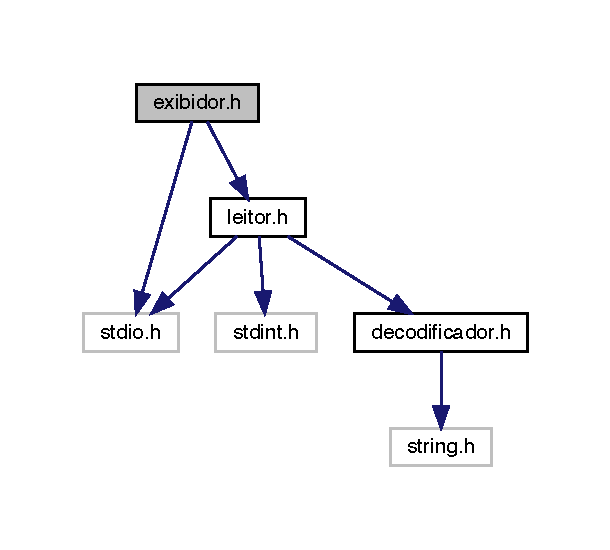
\includegraphics[width=293pt]{exibidor_8h__incl}
\end{center}
\end{figure}
This graph shows which files directly or indirectly include this file\+:
\nopagebreak
\begin{figure}[H]
\begin{center}
\leavevmode
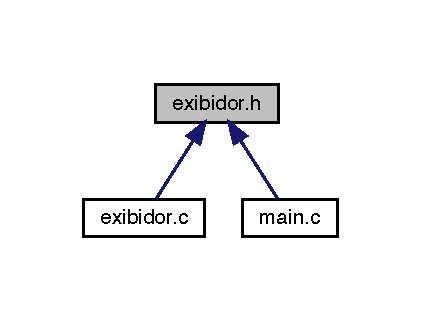
\includegraphics[width=202pt]{exibidor_8h__dep__incl}
\end{center}
\end{figure}
\subsection*{Functions}
\begin{DoxyCompactItemize}
\item 
void \mbox{\hyperlink{exibidor_8h_a157efd9bd041a04a6a6445a4fb44f3fb}{printa\+Class\+File}} (\mbox{\hyperlink{structClassFile}{Class\+File}} $\ast$)
\item 
void \mbox{\hyperlink{exibidor_8h_a67b5fd7cd44ef75d0d99b04ec9212e16}{printa\+Cp\+Info}} (\mbox{\hyperlink{structClassFile}{Class\+File}} $\ast$)
\item 
void \mbox{\hyperlink{exibidor_8h_a80420244c77e051a3960b104550c6072}{printa\+Interfaces}} (\mbox{\hyperlink{structClassFile}{Class\+File}} $\ast$)
\item 
void \mbox{\hyperlink{exibidor_8h_aa3a6d24a57d04f14a7f7650e681ab1df}{printa\+Field\+Info}} (\mbox{\hyperlink{structClassFile}{Class\+File}} $\ast$)
\item 
void \mbox{\hyperlink{exibidor_8h_a75f49b0fb019724ab782731ab9a98d3b}{printa\+Method\+Info}} (\mbox{\hyperlink{structClassFile}{Class\+File}} $\ast$)
\item 
void \mbox{\hyperlink{exibidor_8h_a4c5d4e688928a4cf3a321c6e7d920a23}{printa\+Attribute\+Info}} (\mbox{\hyperlink{structClassFile}{Class\+File}} $\ast$)
\item 
void \mbox{\hyperlink{exibidor_8h_a9803d0a8f19e73f7a21e934261e62750}{imprime\+String\+Pool}} (\mbox{\hyperlink{structCpInfo}{Cp\+Info}} $\ast$, int)
\item 
void \mbox{\hyperlink{exibidor_8h_ab9034805404ccf890d9b6b2b3b4c2e6e}{imprime\+Code}} (\mbox{\hyperlink{structClassFile}{Class\+File}} $\ast$, \mbox{\hyperlink{structCodeAttribute}{Code\+Attribute}} $\ast$)
\item 
void \mbox{\hyperlink{exibidor_8h_ac2ed3e024e89ab7b7987ee91e1b94d80}{imprime\+Exc}} (\mbox{\hyperlink{structClassFile}{Class\+File}} $\ast$, \mbox{\hyperlink{structExceptionsAttribute}{Exceptions\+Attribute}} $\ast$)
\item 
double \mbox{\hyperlink{exibidor_8h_ac3cf42045b984490a357c5368bc560b6}{hex\+To\+Double}} (uint32\+\_\+t, uint32\+\_\+t)
\item 
long \mbox{\hyperlink{exibidor_8h_aab7f8a6f818e47d9768b48419440f92f}{hex\+To\+Long}} (uint32\+\_\+t, uint32\+\_\+t)
\item 
void \mbox{\hyperlink{exibidor_8h_adc96c51c167be415b70fb7091dc22a75}{print\+Access\+Flag}} (uint16\+\_\+t)
\item 
void \mbox{\hyperlink{exibidor_8h_a5ef44612307ac8057846a14bf96edf7f}{imprime\+Major\+Version}} (uint16\+\_\+t)
\item 
\mbox{\Hypertarget{exibidor_8h_a900bd082031766050012dc3b7f348205}\label{exibidor_8h_a900bd082031766050012dc3b7f348205}} 
void {\bfseries print\+Topo} ()
\item 
\mbox{\Hypertarget{exibidor_8h_a5f3fe4937a7bce5015e350ec7588d15b}\label{exibidor_8h_a5f3fe4937a7bce5015e350ec7588d15b}} 
void {\bfseries print\+Blank} ()
\item 
\mbox{\Hypertarget{exibidor_8h_a8579e18db3f0cf53464240c9c8e45a8b}\label{exibidor_8h_a8579e18db3f0cf53464240c9c8e45a8b}} 
void {\bfseries print\+Base} ()
\item 
\mbox{\Hypertarget{exibidor_8h_aa801ec3d076e92418c34fa5e894df667}\label{exibidor_8h_aa801ec3d076e92418c34fa5e894df667}} 
void {\bfseries print\+Single\+Line} ()
\end{DoxyCompactItemize}


\subsection{Function Documentation}
\mbox{\Hypertarget{exibidor_8h_ac3cf42045b984490a357c5368bc560b6}\label{exibidor_8h_ac3cf42045b984490a357c5368bc560b6}} 
\index{exibidor.h@{exibidor.h}!hexToDouble@{hexToDouble}}
\index{hexToDouble@{hexToDouble}!exibidor.h@{exibidor.h}}
\subsubsection{\texorpdfstring{hexToDouble()}{hexToDouble()}}
{\footnotesize\ttfamily double hex\+To\+Double (\begin{DoxyParamCaption}\item[{uint32\+\_\+t}]{high\+Bytes,  }\item[{uint32\+\_\+t}]{low\+Bytes }\end{DoxyParamCaption})}

Funcao converte um valor Hexademical lido em bytes para uma variavel double (tipada de acordo com C99).


\begin{DoxyParams}{Parameters}
{\em uint32\+\_\+t} & Parte alta dos 64 bits \\
\hline
{\em uint32\+\_\+t} & Parte baixa dos 64 bits \\
\hline
\end{DoxyParams}
\begin{DoxyReturn}{Returns}
{\ttfamily double} O valor Hexadecimal de entrada salvo numa variavel do tipo double 
\end{DoxyReturn}
\mbox{\Hypertarget{exibidor_8h_aab7f8a6f818e47d9768b48419440f92f}\label{exibidor_8h_aab7f8a6f818e47d9768b48419440f92f}} 
\index{exibidor.h@{exibidor.h}!hexToLong@{hexToLong}}
\index{hexToLong@{hexToLong}!exibidor.h@{exibidor.h}}
\subsubsection{\texorpdfstring{hexToLong()}{hexToLong()}}
{\footnotesize\ttfamily long hex\+To\+Long (\begin{DoxyParamCaption}\item[{uint32\+\_\+t}]{high\+Bytes,  }\item[{uint32\+\_\+t}]{low\+Bytes }\end{DoxyParamCaption})}

Funcao converte um valor Hexademical lido em bytes para uma variavel long (tipada de acordo com C99).


\begin{DoxyParams}{Parameters}
{\em uint32\+\_\+t} & Parte alta dos 64 bits \\
\hline
{\em uint32\+\_\+t} & Parte baixa dos 64 bits \\
\hline
\end{DoxyParams}
\begin{DoxyReturn}{Returns}
{\ttfamily long} O valor Hexadecimal de entrada salvo numa variavel do tipo long 
\end{DoxyReturn}
\mbox{\Hypertarget{exibidor_8h_ab9034805404ccf890d9b6b2b3b4c2e6e}\label{exibidor_8h_ab9034805404ccf890d9b6b2b3b4c2e6e}} 
\index{exibidor.h@{exibidor.h}!imprimeCode@{imprimeCode}}
\index{imprimeCode@{imprimeCode}!exibidor.h@{exibidor.h}}
\subsubsection{\texorpdfstring{imprimeCode()}{imprimeCode()}}
{\footnotesize\ttfamily void imprime\+Code (\begin{DoxyParamCaption}\item[{\mbox{\hyperlink{structClassFile}{Class\+File}} $\ast$}]{class\+File,  }\item[{\mbox{\hyperlink{structCodeAttribute}{Code\+Attribute}} $\ast$}]{cd\+Atrb }\end{DoxyParamCaption})}

Funcao que imprime as instrucoes (mnemonicos) de um metodo, alem das informacoes sobre o Code do metodo e das referencias de cada valor no Constant Pool.


\begin{DoxyParams}{Parameters}
{\em Class\+File$\ast$} & Ponteiro para a estrutura Classfile \\
\hline
{\em Code\+Attributte$\ast$} & Ponteiro para a estrutura \mbox{\hyperlink{structCodeAttribute}{Code\+Attribute}} \\
\hline
\end{DoxyParams}
\begin{DoxyReturn}{Returns}
{\ttfamily void} 
\end{DoxyReturn}
\begin{DoxySeeAlso}{See also}
print\+Single\+Line \mbox{\hyperlink{exibidor_8c_a779037b6863fb2a2a41e99ab25c04b8d}{imprime\+String\+Pool}} \mbox{\hyperlink{decodificador_8h_a33a5a572beb55160cd59df462a10cdc3}{inicializa\+Decodificador}} 
\end{DoxySeeAlso}
\mbox{\Hypertarget{exibidor_8h_ac2ed3e024e89ab7b7987ee91e1b94d80}\label{exibidor_8h_ac2ed3e024e89ab7b7987ee91e1b94d80}} 
\index{exibidor.h@{exibidor.h}!imprimeExc@{imprimeExc}}
\index{imprimeExc@{imprimeExc}!exibidor.h@{exibidor.h}}
\subsubsection{\texorpdfstring{imprimeExc()}{imprimeExc()}}
{\footnotesize\ttfamily void imprime\+Exc (\begin{DoxyParamCaption}\item[{\mbox{\hyperlink{structClassFile}{Class\+File}} $\ast$}]{class\+File,  }\item[{\mbox{\hyperlink{structExceptionsAttribute}{Exceptions\+Attribute}} $\ast$}]{exc\+Atrb }\end{DoxyParamCaption})}

Funcao que imprime as excecoes (quando especificadas) e as referencias de cada ao Constant Pool.


\begin{DoxyParams}{Parameters}
{\em Class\+File$\ast$} & Ponteiro para a estrutura Classfile \\
\hline
{\em Exceptions\+Attribute$\ast$} & Ponteiro para a estrutura \mbox{\hyperlink{structExceptionsAttribute}{Exceptions\+Attribute}} \\
\hline
\end{DoxyParams}
\begin{DoxyReturn}{Returns}
{\ttfamily void} 
\end{DoxyReturn}
\begin{DoxySeeAlso}{See also}
print\+Single\+Line \mbox{\hyperlink{exibidor_8c_a779037b6863fb2a2a41e99ab25c04b8d}{imprime\+String\+Pool}} 
\end{DoxySeeAlso}
\mbox{\Hypertarget{exibidor_8h_a5ef44612307ac8057846a14bf96edf7f}\label{exibidor_8h_a5ef44612307ac8057846a14bf96edf7f}} 
\index{exibidor.h@{exibidor.h}!imprimeMajorVersion@{imprimeMajorVersion}}
\index{imprimeMajorVersion@{imprimeMajorVersion}!exibidor.h@{exibidor.h}}
\subsubsection{\texorpdfstring{imprimeMajorVersion()}{imprimeMajorVersion()}}
{\footnotesize\ttfamily void imprime\+Major\+Version (\begin{DoxyParamCaption}\item[{uint16\+\_\+t}]{minor }\end{DoxyParamCaption})}

Recebe os bytes de minor version lidos do \mbox{\hyperlink{structClassFile}{Class\+File}} e converte para a versao Java.


\begin{DoxyParams}{Parameters}
{\em uint16\+\_\+t} & 2bytes do minor version \\
\hline
\end{DoxyParams}
\begin{DoxyReturn}{Returns}
{\ttfamily void} 
\end{DoxyReturn}
\mbox{\Hypertarget{exibidor_8h_a9803d0a8f19e73f7a21e934261e62750}\label{exibidor_8h_a9803d0a8f19e73f7a21e934261e62750}} 
\index{exibidor.h@{exibidor.h}!imprimeStringPool@{imprimeStringPool}}
\index{imprimeStringPool@{imprimeStringPool}!exibidor.h@{exibidor.h}}
\subsubsection{\texorpdfstring{imprimeStringPool()}{imprimeStringPool()}}
{\footnotesize\ttfamily void imprime\+String\+Pool (\begin{DoxyParamCaption}\item[{\mbox{\hyperlink{structCpInfo}{Cp\+Info}} $\ast$}]{cp,  }\item[{int}]{pos }\end{DoxyParamCaption})}

Funcao que imprime na tela o U\+T\+F8 final de uma constante a partir de sua posicao. O U\+T\+F8 eh encontrado recursivamente.


\begin{DoxyParams}{Parameters}
{\em Class\+File$\ast$} & Ponteiro para a estrutura Classfile \\
\hline
{\em int} & Posicao da costante que sera impressa \\
\hline
\end{DoxyParams}
\begin{DoxyReturn}{Returns}
{\ttfamily void} 
\end{DoxyReturn}
\mbox{\Hypertarget{exibidor_8h_a4c5d4e688928a4cf3a321c6e7d920a23}\label{exibidor_8h_a4c5d4e688928a4cf3a321c6e7d920a23}} 
\index{exibidor.h@{exibidor.h}!printaAttributeInfo@{printaAttributeInfo}}
\index{printaAttributeInfo@{printaAttributeInfo}!exibidor.h@{exibidor.h}}
\subsubsection{\texorpdfstring{printaAttributeInfo()}{printaAttributeInfo()}}
{\footnotesize\ttfamily void printa\+Attribute\+Info (\begin{DoxyParamCaption}\item[{\mbox{\hyperlink{structClassFile}{Class\+File}} $\ast$}]{class\+File }\end{DoxyParamCaption})}

Funcao que imprime as informacoes dos Atributos da classe, bem como suas referencias no Constant Pool.


\begin{DoxyParams}{Parameters}
{\em Class\+File$\ast$} & Ponteiro para a estrutura Classfile \\
\hline
\end{DoxyParams}
\begin{DoxyReturn}{Returns}
{\ttfamily void} 
\end{DoxyReturn}
\begin{DoxySeeAlso}{See also}
\mbox{\hyperlink{exibidor_8c_a779037b6863fb2a2a41e99ab25c04b8d}{imprime\+String\+Pool}} print\+Single\+Line 
\end{DoxySeeAlso}
\mbox{\Hypertarget{exibidor_8h_adc96c51c167be415b70fb7091dc22a75}\label{exibidor_8h_adc96c51c167be415b70fb7091dc22a75}} 
\index{exibidor.h@{exibidor.h}!printAccessFlag@{printAccessFlag}}
\index{printAccessFlag@{printAccessFlag}!exibidor.h@{exibidor.h}}
\subsubsection{\texorpdfstring{printAccessFlag()}{printAccessFlag()}}
{\footnotesize\ttfamily void print\+Access\+Flag (\begin{DoxyParamCaption}\item[{uint16\+\_\+t}]{access\+Flags }\end{DoxyParamCaption})}

Funcao que imprime o tipo de Access Flag de acordo com o parametro Hexadecimal passado. Se o valor for string com todas as flags eh impressa na tela.


\begin{DoxyParams}{Parameters}
{\em uint16\+\_\+t} & Valor Hexadecimal referente a uma flag ou combinacao de flags \\
\hline
{\em uint32\+\_\+t} & Parte baixa dos 64 bits \\
\hline
\end{DoxyParams}
\begin{DoxyReturn}{Returns}
{\ttfamily void} 
\end{DoxyReturn}
\mbox{\Hypertarget{exibidor_8h_a157efd9bd041a04a6a6445a4fb44f3fb}\label{exibidor_8h_a157efd9bd041a04a6a6445a4fb44f3fb}} 
\index{exibidor.h@{exibidor.h}!printaClassFile@{printaClassFile}}
\index{printaClassFile@{printaClassFile}!exibidor.h@{exibidor.h}}
\subsubsection{\texorpdfstring{printaClassFile()}{printaClassFile()}}
{\footnotesize\ttfamily void printa\+Class\+File (\begin{DoxyParamCaption}\item[{\mbox{\hyperlink{structClassFile}{Class\+File}} $\ast$}]{class\+File }\end{DoxyParamCaption})}

Funcao principal que imprime as informacoes gerais e coordena as chamadas das funcoes que imprimem as demais estuturas do classfile


\begin{DoxyParams}{Parameters}
{\em Class\+File$\ast$} & Ponteiro para a estrutura Classfile \\
\hline
\end{DoxyParams}
\begin{DoxyReturn}{Returns}
{\ttfamily void} 
\end{DoxyReturn}
\begin{DoxySeeAlso}{See also}
\mbox{\hyperlink{exibidor_8c_afccec8f6e6482cf1068555390a62c127}{printa\+Cp\+Info}} \mbox{\hyperlink{exibidor_8c_a97e7f4f9858dd377560e568e6c2f6b69}{printa\+Interfaces}} \mbox{\hyperlink{exibidor_8c_a628a6794abdbb58d9f3a512d8918af23}{printa\+Field\+Info}} \mbox{\hyperlink{exibidor_8c_ad6fba2eba482e4cd9b8e0f4727a1a916}{printa\+Method\+Info}} \mbox{\hyperlink{exibidor_8c_aa1ebe5081deb9425d3a11c9316e3d1ec}{printa\+Attribute\+Info}} 

\mbox{\hyperlink{exibidor_8c_a779037b6863fb2a2a41e99ab25c04b8d}{imprime\+String\+Pool}} print\+Topo print\+Base print\+Blank 
\end{DoxySeeAlso}
\mbox{\Hypertarget{exibidor_8h_a67b5fd7cd44ef75d0d99b04ec9212e16}\label{exibidor_8h_a67b5fd7cd44ef75d0d99b04ec9212e16}} 
\index{exibidor.h@{exibidor.h}!printaCpInfo@{printaCpInfo}}
\index{printaCpInfo@{printaCpInfo}!exibidor.h@{exibidor.h}}
\subsubsection{\texorpdfstring{printaCpInfo()}{printaCpInfo()}}
{\footnotesize\ttfamily void printa\+Cp\+Info (\begin{DoxyParamCaption}\item[{\mbox{\hyperlink{structClassFile}{Class\+File}} $\ast$}]{class\+File }\end{DoxyParamCaption})}

Funcao que imprime o Constant Pool, buscando os valores U\+T\+F8 finais de cada constatnte e imprimindo tambem suas referencias


\begin{DoxyParams}{Parameters}
{\em Class\+File$\ast$} & Ponteiro para a estrutura Classfile \\
\hline
\end{DoxyParams}
\begin{DoxyReturn}{Returns}
{\ttfamily void} 
\end{DoxyReturn}
\begin{DoxySeeAlso}{See also}
\mbox{\hyperlink{exibidor_8c_a779037b6863fb2a2a41e99ab25c04b8d}{imprime\+String\+Pool}} \mbox{\hyperlink{exibidor_8c_ae3623748d39f700f065fc13619af7599}{hex\+To\+Double}} \mbox{\hyperlink{exibidor_8c_a1d10814d2eb259040b2a191921a7878f}{hex\+To\+Long}} 
\end{DoxySeeAlso}
\mbox{\Hypertarget{exibidor_8h_aa3a6d24a57d04f14a7f7650e681ab1df}\label{exibidor_8h_aa3a6d24a57d04f14a7f7650e681ab1df}} 
\index{exibidor.h@{exibidor.h}!printaFieldInfo@{printaFieldInfo}}
\index{printaFieldInfo@{printaFieldInfo}!exibidor.h@{exibidor.h}}
\subsubsection{\texorpdfstring{printaFieldInfo()}{printaFieldInfo()}}
{\footnotesize\ttfamily void printa\+Field\+Info (\begin{DoxyParamCaption}\item[{\mbox{\hyperlink{structClassFile}{Class\+File}} $\ast$}]{class\+File }\end{DoxyParamCaption})}

Funcao que imprime as informacoes de Fields da classe, bem como suas referencias no Constant Pool.


\begin{DoxyParams}{Parameters}
{\em Class\+File$\ast$} & Ponteiro para a estrutura Classfile \\
\hline
\end{DoxyParams}
\begin{DoxyReturn}{Returns}
{\ttfamily void} 
\end{DoxyReturn}
\begin{DoxySeeAlso}{See also}
\mbox{\hyperlink{exibidor_8c_a779037b6863fb2a2a41e99ab25c04b8d}{imprime\+String\+Pool}} \mbox{\hyperlink{exibidor_8c_aa1dcc58c50687652a1eda3b9d99a4496}{print\+Access\+Flag}} print\+Single\+Line 
\end{DoxySeeAlso}
\mbox{\Hypertarget{exibidor_8h_a80420244c77e051a3960b104550c6072}\label{exibidor_8h_a80420244c77e051a3960b104550c6072}} 
\index{exibidor.h@{exibidor.h}!printaInterfaces@{printaInterfaces}}
\index{printaInterfaces@{printaInterfaces}!exibidor.h@{exibidor.h}}
\subsubsection{\texorpdfstring{printaInterfaces()}{printaInterfaces()}}
{\footnotesize\ttfamily void printa\+Interfaces (\begin{DoxyParamCaption}\item[{\mbox{\hyperlink{structClassFile}{Class\+File}} $\ast$}]{class\+File }\end{DoxyParamCaption})}

Funcao que imprime Interfaces da classe passada parametro, alem das referencias das constantes que contem as informacoes U\+T\+F8 de cada Interface


\begin{DoxyParams}{Parameters}
{\em Class\+File$\ast$} & Ponteiro para a estrutura Classfile \\
\hline
\end{DoxyParams}
\begin{DoxyReturn}{Returns}
{\ttfamily void} 
\end{DoxyReturn}
\begin{DoxySeeAlso}{See also}
\mbox{\hyperlink{exibidor_8c_a779037b6863fb2a2a41e99ab25c04b8d}{imprime\+String\+Pool}} 
\end{DoxySeeAlso}
\mbox{\Hypertarget{exibidor_8h_a75f49b0fb019724ab782731ab9a98d3b}\label{exibidor_8h_a75f49b0fb019724ab782731ab9a98d3b}} 
\index{exibidor.h@{exibidor.h}!printaMethodInfo@{printaMethodInfo}}
\index{printaMethodInfo@{printaMethodInfo}!exibidor.h@{exibidor.h}}
\subsubsection{\texorpdfstring{printaMethodInfo()}{printaMethodInfo()}}
{\footnotesize\ttfamily void printa\+Method\+Info (\begin{DoxyParamCaption}\item[{\mbox{\hyperlink{structClassFile}{Class\+File}} $\ast$}]{class\+File }\end{DoxyParamCaption})}

Funcao que imprime as informacoes dos Metodos da classe, suas instrucoes (mnemonicos) e suas referencias no Constant Pool.


\begin{DoxyParams}{Parameters}
{\em Class\+File$\ast$} & Ponteiro para a estrutura Classfile \\
\hline
\end{DoxyParams}
\begin{DoxyReturn}{Returns}
{\ttfamily void} 
\end{DoxyReturn}
\begin{DoxySeeAlso}{See also}
\mbox{\hyperlink{exibidor_8c_a779037b6863fb2a2a41e99ab25c04b8d}{imprime\+String\+Pool}} \mbox{\hyperlink{exibidor_8c_a7c0475d7e6531aa7a07e7f1103fc56e0}{imprime\+Code}} \mbox{\hyperlink{exibidor_8c_a9d4be7efdb4277ecb2294302e9d35b37}{imprime\+Exc}} 
\end{DoxySeeAlso}

\hypertarget{frame_8c}{}\section{frame.\+c File Reference}
\label{frame_8c}\index{frame.\+c@{frame.\+c}}


Gerenciamento e alocação de memória das frames do programa executado.  


{\ttfamily \#include \char`\"{}frame.\+h\char`\"{}}\newline
Include dependency graph for frame.\+c\+:
% FIG 0
\subsection*{Functions}
\begin{DoxyCompactItemize}
\item 
void \hyperlink{frame_8c_a043120e5dc10c5874fafd5b92506dd54}{cria\+Frame} (\hyperlink{structClassFile}{Class\+File} $\ast$classe, \hyperlink{structCodeAttribute}{Code\+Attribute} $\ast$code\+Attribute)
\item 
void \hyperlink{frame_8c_a71c5d25687de0a2568a6cf7c62dfef26}{push\+Frame} (\hyperlink{structClassFile}{Class\+File} $\ast$classe, \hyperlink{structCodeAttribute}{Code\+Attribute} $\ast$code\+Attribute, \hyperlink{structStackFrame}{Stack\+Frame} $\ast$stack\+Frame)
\item 
void \hyperlink{frame_8c_aca9cbfa46eaa4e3c07217b16d0c5212e}{pop\+Frame} ()
\item 
void \hyperlink{frame_8c_a50993c39467516396b64a90eb81af0ba}{push\+Op} (int32\+\_\+t valor)
\item 
int32\+\_\+t \hyperlink{frame_8c_a3670f378856724ca85ced056e6bfc5c4}{pop\+Op} ()
\item 
int \hyperlink{frame_8c_a4a14b8e8d6925b6383b12597cb8a4dc1}{checka\+Overflow\+Pilha\+Op} ()
\item 
int \hyperlink{frame_8c_a7ea50bc48f670ca5ef7573e4256c213c}{checka\+Underflow\+Pilha\+Op} ()
\end{DoxyCompactItemize}
\subsection*{Variables}
\begin{DoxyCompactItemize}
\item 
\mbox{\Hypertarget{frame_8c_a352d20cc1b440fd3e25d463b5e2efdb4}\label{frame_8c_a352d20cc1b440fd3e25d463b5e2efdb4}} 
\hyperlink{structDecodificador}{Decodificador} {\bfseries dec} \mbox{[}N\+U\+M\+\_\+\+I\+N\+S\+T\+R\+U\+C\+AO\mbox{]}
\item 
\mbox{\Hypertarget{frame_8c_aad62b45c5a0a8993d540ec7b83ef02ee}\label{frame_8c_aad62b45c5a0a8993d540ec7b83ef02ee}} 
\hyperlink{structFrame}{Frame} $\ast$ {\bfseries frame\+Corrente}
\item 
\mbox{\Hypertarget{frame_8c_a41b21f484ed1e3efce18dcb9a07ae865}\label{frame_8c_a41b21f484ed1e3efce18dcb9a07ae865}} 
int32\+\_\+t {\bfseries qtd\+Arrays}
\end{DoxyCompactItemize}


\subsection{Detailed Description}
Gerenciamento e alocação de memória das frames do programa executado. 

\begin{DoxyAuthor}{Authors}
Bruno Sanguinetti 18/0046063 ~\newline
Gabriel Vasconcelos 16/0120781 ~\newline
Leonardo de Almeida 15/0135491 ~\newline
Lucas Mafra 12/0126443 ~\newline
Wladimir Gramacho 15/0058718 ~\newline
 
\end{DoxyAuthor}
\begin{DoxyDate}{Date}
28/06/2017
\end{DoxyDate}
\begin{DoxyCopyright}{Copyright}
Copyright © 2017 Grupo\+SB. All rights reserved. 
\end{DoxyCopyright}


\subsection{Function Documentation}
\mbox{\Hypertarget{frame_8c_a4a14b8e8d6925b6383b12597cb8a4dc1}\label{frame_8c_a4a14b8e8d6925b6383b12597cb8a4dc1}} 
\index{frame.\+c@{frame.\+c}!checka\+Overflow\+Pilha\+Op@{checka\+Overflow\+Pilha\+Op}}
\index{checka\+Overflow\+Pilha\+Op@{checka\+Overflow\+Pilha\+Op}!frame.\+c@{frame.\+c}}
\subsubsection{\texorpdfstring{checka\+Overflow\+Pilha\+Op()}{checkaOverflowPilhaOp()}}
{\footnotesize\ttfamily int checka\+Overflow\+Pilha\+Op (\begin{DoxyParamCaption}{ }\end{DoxyParamCaption})}

Confere se o tamanho da pilha excedeu o tamanho maximo (max stack)


\begin{DoxyParams}{Parameters}
{\em Nao} & possui parametros. \\
\hline
\end{DoxyParams}
\begin{DoxyReturn}{Returns}
{\ttfamily int} Resultado de uma comparacao (0 ou 1) 
\end{DoxyReturn}
\mbox{\Hypertarget{frame_8c_a7ea50bc48f670ca5ef7573e4256c213c}\label{frame_8c_a7ea50bc48f670ca5ef7573e4256c213c}} 
\index{frame.\+c@{frame.\+c}!checka\+Underflow\+Pilha\+Op@{checka\+Underflow\+Pilha\+Op}}
\index{checka\+Underflow\+Pilha\+Op@{checka\+Underflow\+Pilha\+Op}!frame.\+c@{frame.\+c}}
\subsubsection{\texorpdfstring{checka\+Underflow\+Pilha\+Op()}{checkaUnderflowPilhaOp()}}
{\footnotesize\ttfamily int checka\+Underflow\+Pilha\+Op (\begin{DoxyParamCaption}{ }\end{DoxyParamCaption})}

Confere se a profundidade da pilha esta negativa.


\begin{DoxyParams}{Parameters}
{\em Nao} & possui parametros. \\
\hline
\end{DoxyParams}
\begin{DoxyReturn}{Returns}
{\ttfamily int} Resultado de uma comparacao (0 ou 1) 
\end{DoxyReturn}
\mbox{\Hypertarget{frame_8c_a043120e5dc10c5874fafd5b92506dd54}\label{frame_8c_a043120e5dc10c5874fafd5b92506dd54}} 
\index{frame.\+c@{frame.\+c}!cria\+Frame@{cria\+Frame}}
\index{cria\+Frame@{cria\+Frame}!frame.\+c@{frame.\+c}}
\subsubsection{\texorpdfstring{cria\+Frame()}{criaFrame()}}
{\footnotesize\ttfamily void cria\+Frame (\begin{DoxyParamCaption}\item[{\hyperlink{structClassFile}{Class\+File} $\ast$}]{classe,  }\item[{\hyperlink{structCodeAttribute}{Code\+Attribute} $\ast$}]{code\+Attribute }\end{DoxyParamCaption})}

Cria um frame e coloca ele na pilha de frames.


\begin{DoxyParams}{Parameters}
{\em Class\+File$\ast$} & Ponteiro para a estrutura \hyperlink{structClassFile}{Class\+File}. \\
\hline
{\em Code\+Attribute$\ast$} & Ponteiro para a estrutura \hyperlink{structCodeAttribute}{Code\+Attribute}. \\
\hline
\end{DoxyParams}
\begin{DoxyReturn}{Returns}
{\ttfamily void} 
\end{DoxyReturn}
\begin{DoxySeeAlso}{See also}
\hyperlink{frame_8c_a71c5d25687de0a2568a6cf7c62dfef26}{push\+Frame} 
\end{DoxySeeAlso}
\mbox{\Hypertarget{frame_8c_aca9cbfa46eaa4e3c07217b16d0c5212e}\label{frame_8c_aca9cbfa46eaa4e3c07217b16d0c5212e}} 
\index{frame.\+c@{frame.\+c}!pop\+Frame@{pop\+Frame}}
\index{pop\+Frame@{pop\+Frame}!frame.\+c@{frame.\+c}}
\subsubsection{\texorpdfstring{pop\+Frame()}{popFrame()}}
{\footnotesize\ttfamily void pop\+Frame (\begin{DoxyParamCaption}{ }\end{DoxyParamCaption})}

Retira um frame da pilha de frames e atualiza o topo da pilha.


\begin{DoxyParams}{Parameters}
{\em Nao} & possui parametros \\
\hline
\end{DoxyParams}
\begin{DoxyReturn}{Returns}
{\ttfamily void} 
\end{DoxyReturn}
\begin{DoxySeeAlso}{See also}
\hyperlink{frame_8c_a50993c39467516396b64a90eb81af0ba}{push\+Op} 
\end{DoxySeeAlso}
\mbox{\Hypertarget{frame_8c_a3670f378856724ca85ced056e6bfc5c4}\label{frame_8c_a3670f378856724ca85ced056e6bfc5c4}} 
\index{frame.\+c@{frame.\+c}!pop\+Op@{pop\+Op}}
\index{pop\+Op@{pop\+Op}!frame.\+c@{frame.\+c}}
\subsubsection{\texorpdfstring{pop\+Op()}{popOp()}}
{\footnotesize\ttfamily int32\+\_\+t pop\+Op (\begin{DoxyParamCaption}{ }\end{DoxyParamCaption})}

Desempilha um valor na pilha de operandos.


\begin{DoxyParams}{Parameters}
{\em Nao} & possui parametros. \\
\hline
\end{DoxyParams}
\begin{DoxyReturn}{Returns}
{\ttfamily int32\+\_\+t} Retorna o valor desempilhado da pilha de operandos. 
\end{DoxyReturn}
\mbox{\Hypertarget{frame_8c_a71c5d25687de0a2568a6cf7c62dfef26}\label{frame_8c_a71c5d25687de0a2568a6cf7c62dfef26}} 
\index{frame.\+c@{frame.\+c}!push\+Frame@{push\+Frame}}
\index{push\+Frame@{push\+Frame}!frame.\+c@{frame.\+c}}
\subsubsection{\texorpdfstring{push\+Frame()}{pushFrame()}}
{\footnotesize\ttfamily void push\+Frame (\begin{DoxyParamCaption}\item[{\hyperlink{structClassFile}{Class\+File} $\ast$}]{classe,  }\item[{\hyperlink{structCodeAttribute}{Code\+Attribute} $\ast$}]{code\+Attribute,  }\item[{\hyperlink{structStackFrame}{Stack\+Frame} $\ast$}]{stack\+Frame }\end{DoxyParamCaption})}

Coloca o frame passado por parametro na pilha de frames e atualiza o topo da pilha.


\begin{DoxyParams}{Parameters}
{\em Class\+File$\ast$} & Ponteiro para a estrutura \hyperlink{structClassFile}{Class\+File}. \\
\hline
{\em Code\+Attribute$\ast$} & Ponteiro para a estrutura \hyperlink{structCodeAttribute}{Code\+Attribute}. \\
\hline
{\em Stack\+Frame$\ast$} & Ponteiro para a estrutura \hyperlink{structStackFrame}{Stack\+Frame} \\
\hline
\end{DoxyParams}
\begin{DoxyReturn}{Returns}
{\ttfamily void} 
\end{DoxyReturn}
\mbox{\Hypertarget{frame_8c_a50993c39467516396b64a90eb81af0ba}\label{frame_8c_a50993c39467516396b64a90eb81af0ba}} 
\index{frame.\+c@{frame.\+c}!push\+Op@{push\+Op}}
\index{push\+Op@{push\+Op}!frame.\+c@{frame.\+c}}
\subsubsection{\texorpdfstring{push\+Op()}{pushOp()}}
{\footnotesize\ttfamily void push\+Op (\begin{DoxyParamCaption}\item[{int32\+\_\+t}]{valor }\end{DoxyParamCaption})}

Empilha um valor na pilha de operandos.


\begin{DoxyParams}{Parameters}
{\em int32\+\_\+t} & Valor a ser inserido na pilha de operandos. \\
\hline
\end{DoxyParams}
\begin{DoxyReturn}{Returns}
{\ttfamily void} 
\end{DoxyReturn}

\hypertarget{frame_8h}{}\section{frame.\+h File Reference}
\label{frame_8h}\index{frame.h@{frame.h}}
{\ttfamily \#include $<$stdint.\+h$>$}\newline
{\ttfamily \#include $<$stdlib.\+h$>$}\newline
{\ttfamily \#include \char`\"{}leitor.\+h\char`\"{}}\newline
Include dependency graph for frame.\+h\+:
\nopagebreak
\begin{figure}[H]
\begin{center}
\leavevmode
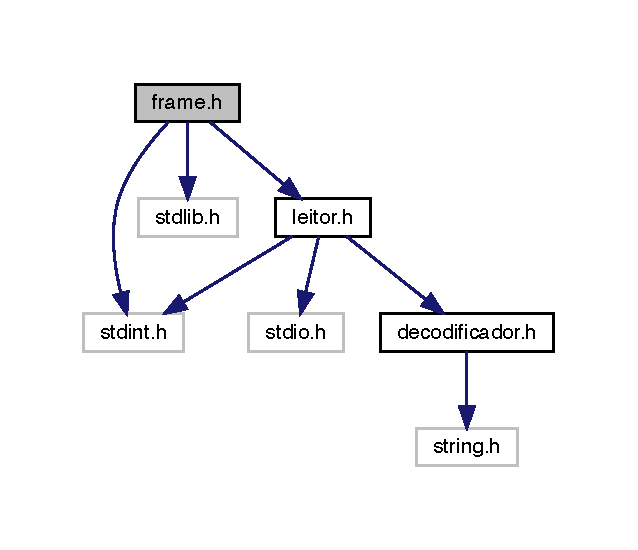
\includegraphics[width=306pt]{frame_8h__incl}
\end{center}
\end{figure}
This graph shows which files directly or indirectly include this file\+:
\nopagebreak
\begin{figure}[H]
\begin{center}
\leavevmode
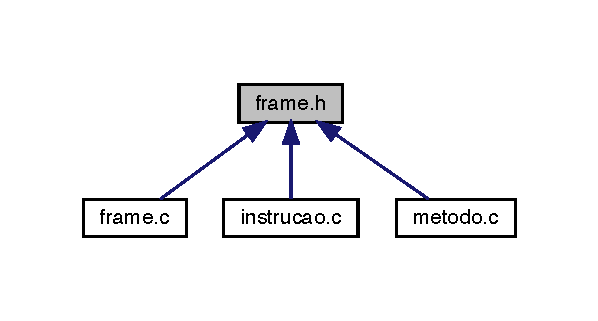
\includegraphics[width=287pt]{frame_8h__dep__incl}
\end{center}
\end{figure}
\subsection*{Classes}
\begin{DoxyCompactItemize}
\item 
struct \mbox{\hyperlink{structPilhaOp}{Pilha\+Op}}
\item 
struct \mbox{\hyperlink{structFrame}{Frame}}
\item 
struct \mbox{\hyperlink{structStackFrame}{Stack\+Frame}}
\item 
struct \mbox{\hyperlink{structVector}{Vector}}
\end{DoxyCompactItemize}
\subsection*{Typedefs}
\begin{DoxyCompactItemize}
\item 
\mbox{\Hypertarget{frame_8h_a2d17b34734bf257b279535e064833f3f}\label{frame_8h_a2d17b34734bf257b279535e064833f3f}} 
typedef struct \mbox{\hyperlink{structPilhaOp}{Pilha\+Op}} {\bfseries Pilha\+Op}
\item 
\mbox{\Hypertarget{frame_8h_a2a5c56d9766cd18277c4c9430518b326}\label{frame_8h_a2a5c56d9766cd18277c4c9430518b326}} 
typedef struct \mbox{\hyperlink{structFrame}{Frame}} {\bfseries Frame}
\item 
\mbox{\Hypertarget{frame_8h_a0b2bdc4691a7ecce810a6639f1aee20a}\label{frame_8h_a0b2bdc4691a7ecce810a6639f1aee20a}} 
typedef struct \mbox{\hyperlink{structStackFrame}{Stack\+Frame}} {\bfseries Stack\+Frame}
\item 
\mbox{\Hypertarget{frame_8h_a6ded2cf071c127e518317e3c451af3ef}\label{frame_8h_a6ded2cf071c127e518317e3c451af3ef}} 
typedef struct \mbox{\hyperlink{structVector}{Vector}} {\bfseries Vector}
\end{DoxyCompactItemize}
\subsection*{Functions}
\begin{DoxyCompactItemize}
\item 
int32\+\_\+t \mbox{\hyperlink{frame_8h_a3670f378856724ca85ced056e6bfc5c4}{pop\+Op}} ()
\item 
void \mbox{\hyperlink{frame_8h_aaad5adf20f46c878f963035a8fb53a70}{cria\+Frame}} (\mbox{\hyperlink{structClassFile}{Class\+File}} $\ast$, \mbox{\hyperlink{structCodeAttribute}{Code\+Attribute}} $\ast$)
\item 
\mbox{\Hypertarget{frame_8h_afbeae238f4237be83cc60071a8a6384d}\label{frame_8h_afbeae238f4237be83cc60071a8a6384d}} 
void {\bfseries desaloca\+Frame} ()
\item 
void \mbox{\hyperlink{frame_8h_a163ac593cc4380f51ce48a1072b1bf41}{push\+Op}} (int32\+\_\+t)
\item 
\mbox{\Hypertarget{frame_8h_a66a49a1024974e095ed46edaad769052}\label{frame_8h_a66a49a1024974e095ed46edaad769052}} 
void {\bfseries dump\+Stack} ()
\item 
\mbox{\Hypertarget{frame_8h_a26b0bade701040dce261d302f608ed60}\label{frame_8h_a26b0bade701040dce261d302f608ed60}} 
void {\bfseries dump\+Fields} ()
\item 
void \mbox{\hyperlink{frame_8h_a6c316e194f496f983e3b330020df4222}{push\+Frame}} (\mbox{\hyperlink{structClassFile}{Class\+File}} $\ast$, \mbox{\hyperlink{structCodeAttribute}{Code\+Attribute}} $\ast$, \mbox{\hyperlink{structStackFrame}{Stack\+Frame}} $\ast$)
\item 
void \mbox{\hyperlink{frame_8h_aca9cbfa46eaa4e3c07217b16d0c5212e}{pop\+Frame}} ()
\item 
int \mbox{\hyperlink{frame_8h_a4a14b8e8d6925b6383b12597cb8a4dc1}{checka\+Overflow\+Pilha\+Op}} ()
\item 
int \mbox{\hyperlink{frame_8h_a7ea50bc48f670ca5ef7573e4256c213c}{checka\+Underflow\+Pilha\+Op}} ()
\end{DoxyCompactItemize}
\subsection*{Variables}
\begin{DoxyCompactItemize}
\item 
\mbox{\Hypertarget{frame_8h_ac1c027226ea84b3fcf8eb5e5fbd99d77}\label{frame_8h_ac1c027226ea84b3fcf8eb5e5fbd99d77}} 
int32\+\_\+t {\bfseries retorno}
\item 
\mbox{\Hypertarget{frame_8h_ae095c61cae78465ab2ae26cd68fb239e}\label{frame_8h_ae095c61cae78465ab2ae26cd68fb239e}} 
int32\+\_\+t {\bfseries ret\+Alta}
\item 
\mbox{\Hypertarget{frame_8h_ae2b60b499c926208b8f46565764dfd3e}\label{frame_8h_ae2b60b499c926208b8f46565764dfd3e}} 
int32\+\_\+t {\bfseries ret\+Baixa}
\item 
\mbox{\Hypertarget{frame_8h_a4b4d07f1b803132aeca7f2ee073ec3c8}\label{frame_8h_a4b4d07f1b803132aeca7f2ee073ec3c8}} 
int8\+\_\+t {\bfseries flag\+Ret}
\end{DoxyCompactItemize}


\subsection{Function Documentation}
\mbox{\Hypertarget{frame_8h_a4a14b8e8d6925b6383b12597cb8a4dc1}\label{frame_8h_a4a14b8e8d6925b6383b12597cb8a4dc1}} 
\index{frame.h@{frame.h}!checkaOverflowPilhaOp@{checkaOverflowPilhaOp}}
\index{checkaOverflowPilhaOp@{checkaOverflowPilhaOp}!frame.h@{frame.h}}
\subsubsection{\texorpdfstring{checkaOverflowPilhaOp()}{checkaOverflowPilhaOp()}}
{\footnotesize\ttfamily int checka\+Overflow\+Pilha\+Op (\begin{DoxyParamCaption}{ }\end{DoxyParamCaption})}

Confere se o tamanho da pilha excedeu o tamanho maximo (max stack)


\begin{DoxyParams}{Parameters}
{\em Nao} & possui parametros. \\
\hline
\end{DoxyParams}
\begin{DoxyReturn}{Returns}
{\ttfamily int} Resultado de uma comparacao (0 ou 1) 
\end{DoxyReturn}
\mbox{\Hypertarget{frame_8h_a7ea50bc48f670ca5ef7573e4256c213c}\label{frame_8h_a7ea50bc48f670ca5ef7573e4256c213c}} 
\index{frame.h@{frame.h}!checkaUnderflowPilhaOp@{checkaUnderflowPilhaOp}}
\index{checkaUnderflowPilhaOp@{checkaUnderflowPilhaOp}!frame.h@{frame.h}}
\subsubsection{\texorpdfstring{checkaUnderflowPilhaOp()}{checkaUnderflowPilhaOp()}}
{\footnotesize\ttfamily int checka\+Underflow\+Pilha\+Op (\begin{DoxyParamCaption}{ }\end{DoxyParamCaption})}

Confere se a profundidade da pilha esta negativa.


\begin{DoxyParams}{Parameters}
{\em Nao} & possui parametros. \\
\hline
\end{DoxyParams}
\begin{DoxyReturn}{Returns}
{\ttfamily int} Resultado de uma comparacao (0 ou 1) 
\end{DoxyReturn}
\mbox{\Hypertarget{frame_8h_aaad5adf20f46c878f963035a8fb53a70}\label{frame_8h_aaad5adf20f46c878f963035a8fb53a70}} 
\index{frame.h@{frame.h}!criaFrame@{criaFrame}}
\index{criaFrame@{criaFrame}!frame.h@{frame.h}}
\subsubsection{\texorpdfstring{criaFrame()}{criaFrame()}}
{\footnotesize\ttfamily void cria\+Frame (\begin{DoxyParamCaption}\item[{\mbox{\hyperlink{structClassFile}{Class\+File}} $\ast$}]{classe,  }\item[{\mbox{\hyperlink{structCodeAttribute}{Code\+Attribute}} $\ast$}]{code\+Attribute }\end{DoxyParamCaption})}

Cria um frame e coloca ele na pilha de frames.


\begin{DoxyParams}{Parameters}
{\em Class\+File$\ast$} & Ponteiro para a estrutura \mbox{\hyperlink{structClassFile}{Class\+File}}. \\
\hline
{\em Code\+Attribute$\ast$} & Ponteiro para a estrutura \mbox{\hyperlink{structCodeAttribute}{Code\+Attribute}}. \\
\hline
\end{DoxyParams}
\begin{DoxyReturn}{Returns}
{\ttfamily void} 
\end{DoxyReturn}
\begin{DoxySeeAlso}{See also}
\mbox{\hyperlink{frame_8c_a71c5d25687de0a2568a6cf7c62dfef26}{push\+Frame}} 
\end{DoxySeeAlso}
\mbox{\Hypertarget{frame_8h_aca9cbfa46eaa4e3c07217b16d0c5212e}\label{frame_8h_aca9cbfa46eaa4e3c07217b16d0c5212e}} 
\index{frame.h@{frame.h}!popFrame@{popFrame}}
\index{popFrame@{popFrame}!frame.h@{frame.h}}
\subsubsection{\texorpdfstring{popFrame()}{popFrame()}}
{\footnotesize\ttfamily void pop\+Frame (\begin{DoxyParamCaption}{ }\end{DoxyParamCaption})}

Retira um frame da pilha de frames e atualiza o topo da pilha.


\begin{DoxyParams}{Parameters}
{\em Nao} & possui parametros \\
\hline
\end{DoxyParams}
\begin{DoxyReturn}{Returns}
{\ttfamily void} 
\end{DoxyReturn}
\begin{DoxySeeAlso}{See also}
\mbox{\hyperlink{frame_8c_a50993c39467516396b64a90eb81af0ba}{push\+Op}} 
\end{DoxySeeAlso}
\mbox{\Hypertarget{frame_8h_a3670f378856724ca85ced056e6bfc5c4}\label{frame_8h_a3670f378856724ca85ced056e6bfc5c4}} 
\index{frame.h@{frame.h}!popOp@{popOp}}
\index{popOp@{popOp}!frame.h@{frame.h}}
\subsubsection{\texorpdfstring{popOp()}{popOp()}}
{\footnotesize\ttfamily int32\+\_\+t pop\+Op (\begin{DoxyParamCaption}{ }\end{DoxyParamCaption})}

Desempilha um valor na pilha de operandos.


\begin{DoxyParams}{Parameters}
{\em Nao} & possui parametros. \\
\hline
\end{DoxyParams}
\begin{DoxyReturn}{Returns}
{\ttfamily int32\+\_\+t} Retorna o valor desempilhado da pilha de operandos. 
\end{DoxyReturn}
\mbox{\Hypertarget{frame_8h_a6c316e194f496f983e3b330020df4222}\label{frame_8h_a6c316e194f496f983e3b330020df4222}} 
\index{frame.h@{frame.h}!pushFrame@{pushFrame}}
\index{pushFrame@{pushFrame}!frame.h@{frame.h}}
\subsubsection{\texorpdfstring{pushFrame()}{pushFrame()}}
{\footnotesize\ttfamily void push\+Frame (\begin{DoxyParamCaption}\item[{\mbox{\hyperlink{structClassFile}{Class\+File}} $\ast$}]{classe,  }\item[{\mbox{\hyperlink{structCodeAttribute}{Code\+Attribute}} $\ast$}]{code\+Attribute,  }\item[{\mbox{\hyperlink{structStackFrame}{Stack\+Frame}} $\ast$}]{stack\+Frame }\end{DoxyParamCaption})}

Coloca o frame passado por parametro na pilha de frames e atualiza o topo da pilha.


\begin{DoxyParams}{Parameters}
{\em Class\+File$\ast$} & Ponteiro para a estrutura \mbox{\hyperlink{structClassFile}{Class\+File}}. \\
\hline
{\em Code\+Attribute$\ast$} & Ponteiro para a estrutura \mbox{\hyperlink{structCodeAttribute}{Code\+Attribute}}. \\
\hline
{\em Stack\+Frame$\ast$} & Ponteiro para a estrutura \mbox{\hyperlink{structStackFrame}{Stack\+Frame}} \\
\hline
\end{DoxyParams}
\begin{DoxyReturn}{Returns}
{\ttfamily void} 
\end{DoxyReturn}
\mbox{\Hypertarget{frame_8h_a163ac593cc4380f51ce48a1072b1bf41}\label{frame_8h_a163ac593cc4380f51ce48a1072b1bf41}} 
\index{frame.h@{frame.h}!pushOp@{pushOp}}
\index{pushOp@{pushOp}!frame.h@{frame.h}}
\subsubsection{\texorpdfstring{pushOp()}{pushOp()}}
{\footnotesize\ttfamily void push\+Op (\begin{DoxyParamCaption}\item[{int32\+\_\+t}]{valor }\end{DoxyParamCaption})}

Empilha um valor na pilha de operandos.


\begin{DoxyParams}{Parameters}
{\em int32\+\_\+t} & Valor a ser inserido na pilha de operandos. \\
\hline
\end{DoxyParams}
\begin{DoxyReturn}{Returns}
{\ttfamily void} 
\end{DoxyReturn}

\hypertarget{instrucao_8c}{}\section{instrucao.\+c File Reference}
\label{instrucao_8c}\index{instrucao.c@{instrucao.c}}


Define, interpreta e executa as instruções do programa sendo executado.  


{\ttfamily \#include \char`\"{}instrucao.\+h\char`\"{}}\newline
{\ttfamily \#include \char`\"{}frame.\+h\char`\"{}}\newline
{\ttfamily \#include \char`\"{}carregador.\+h\char`\"{}}\newline
{\ttfamily \#include \char`\"{}area\+Metodos.\+h\char`\"{}}\newline
{\ttfamily \#include \char`\"{}metodo.\+h\char`\"{}}\newline
{\ttfamily \#include $<$stdio.\+h$>$}\newline
{\ttfamily \#include $<$math.\+h$>$}\newline
{\ttfamily \#include $<$stdint.\+h$>$}\newline
{\ttfamily \#include $<$stdlib.\+h$>$}\newline
{\ttfamily \#include $<$inttypes.\+h$>$}\newline
Include dependency graph for instrucao.\+c\+:
\nopagebreak
\begin{figure}[H]
\begin{center}
\leavevmode
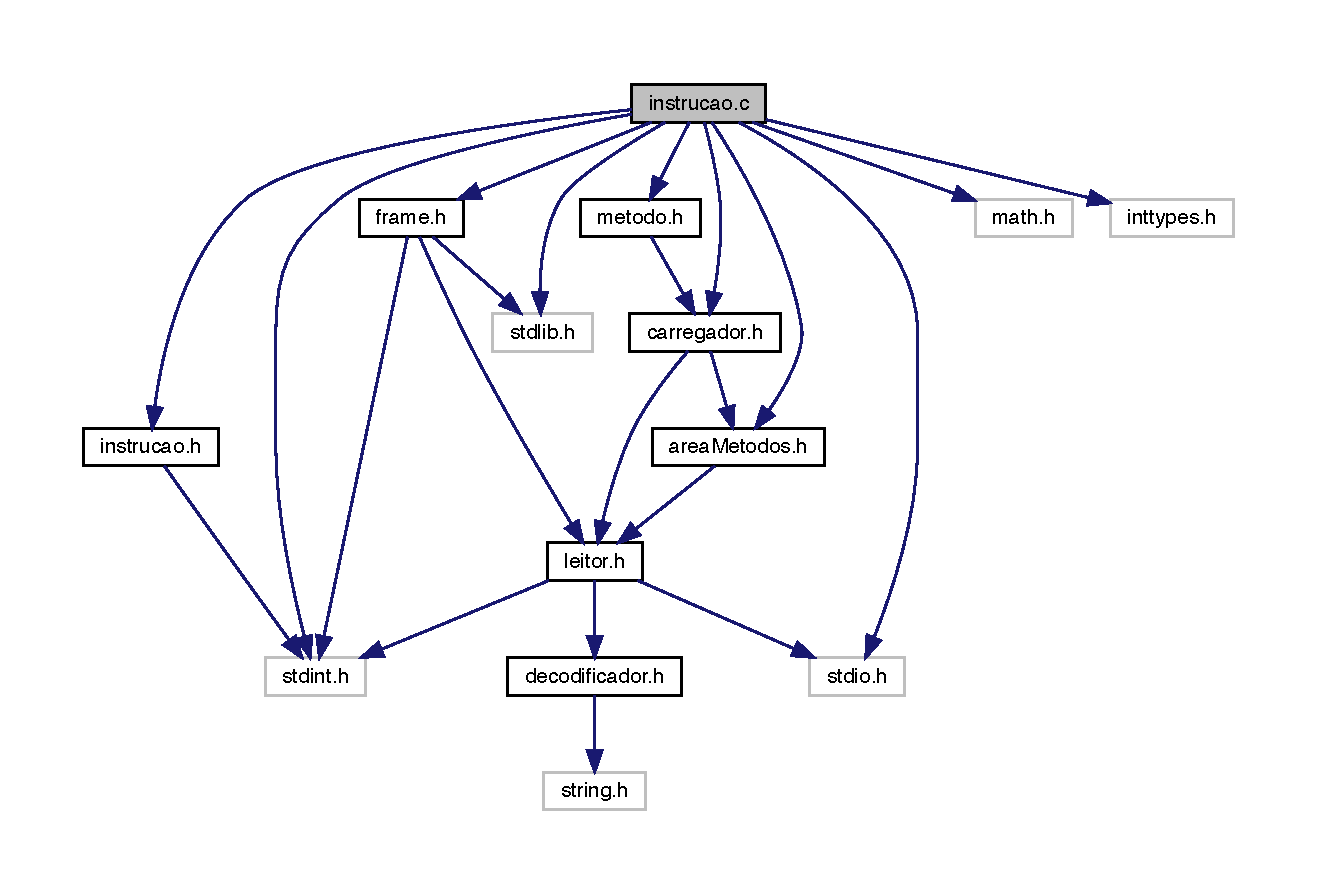
\includegraphics[width=350pt]{instrucao_8c__incl}
\end{center}
\end{figure}
\subsection*{Functions}
\begin{DoxyCompactItemize}
\item 
void \mbox{\hyperlink{instrucao_8c_abcf4bbde1212f9bb0f2ee7a6ba5aec08}{atualiza\+Pc}} ()
\item 
int \mbox{\hyperlink{instrucao_8c_aaebdb63984789b9347c56a436e6a2ef4}{resolve\+U\+TF}} (\mbox{\hyperlink{structCpInfo}{Cp\+Info}} $\ast$cp, int pos\+Pool)
\item 
void \mbox{\hyperlink{instrucao_8c_a308f4b87fb42ab5a62790c0127003ebe}{inicializa\+Instrucoes}} ()
\item 
void \mbox{\hyperlink{instrucao_8c_a9feb7476507383309c8e3ff2648016f3}{nop}} ()
\item 
void \mbox{\hyperlink{instrucao_8c_abe6dd55d61a71f86f8039f4e2d1d00c8}{aconst\+\_\+null}} ()
\item 
void \mbox{\hyperlink{instrucao_8c_a3d4fe47d548d6189745787177183c38c}{iconst\+\_\+m1}} ()
\item 
void \mbox{\hyperlink{instrucao_8c_aea322ceba1bd8d3ef7f33273d58e6f0b}{iconst\+\_\+0}} ()
\item 
void \mbox{\hyperlink{instrucao_8c_ad99980f3110041de270ec04c53107b8f}{iconst\+\_\+1}} ()
\item 
void \mbox{\hyperlink{instrucao_8c_ade068b77731b687d290ff8110b5111fb}{iconst\+\_\+2}} ()
\item 
void \mbox{\hyperlink{instrucao_8c_aa4de912d11b59f82deba1dc335d69123}{iconst\+\_\+3}} ()
\item 
void \mbox{\hyperlink{instrucao_8c_a8c772a238a36dc3c353206ec51a65382}{iconst\+\_\+4}} ()
\item 
void \mbox{\hyperlink{instrucao_8c_a2e5a16634b3e5c00d324b462ea77183b}{iconst\+\_\+5}} ()
\item 
void \mbox{\hyperlink{instrucao_8c_a404bc01bc13afddc52495b6a77a2ff4d}{lconst\+\_\+0}} ()
\item 
void \mbox{\hyperlink{instrucao_8c_a47ef909a27b1a683c8941d87f542b162}{lconst\+\_\+1}} ()
\item 
void \mbox{\hyperlink{instrucao_8c_a86f714d43e3b969d5c30dbfdabd472bf}{fconst\+\_\+0}} ()
\item 
void \mbox{\hyperlink{instrucao_8c_ab87ae6df1b95fd3c3829af30ba899199}{fconst\+\_\+1}} ()
\item 
void \mbox{\hyperlink{instrucao_8c_aa2c5e3ce6d5b8daf54213367d7f02f25}{fconst\+\_\+2}} ()
\item 
void \mbox{\hyperlink{instrucao_8c_a06b623842362ff5bad4321bd3901c041}{dconst\+\_\+0}} ()
\item 
void \mbox{\hyperlink{instrucao_8c_a7f89f5063a41ce732da654abce7f1c81}{dconst\+\_\+1}} ()
\item 
void \mbox{\hyperlink{instrucao_8c_a63e60d614254aaf759e91850ce33be71}{bipush}} ()
\item 
void \mbox{\hyperlink{instrucao_8c_ab232b871bc72922db8f077fc3f356348}{sipush}} ()
\item 
void \mbox{\hyperlink{instrucao_8c_a05601922d5b1a9203cd26a1a21789255}{ldc}} ()
\item 
void \mbox{\hyperlink{instrucao_8c_a24bf1524b99a783375f26b5e4f79fb44}{ldc\+\_\+w}} ()
\item 
void \mbox{\hyperlink{instrucao_8c_ae507168e021393f8ee28cf11c80e5349}{ldc2\+\_\+w}} ()
\item 
void \mbox{\hyperlink{instrucao_8c_a30a4061a47793773606ff72c0b81ddb1}{iload}} ()
\item 
void \mbox{\hyperlink{instrucao_8c_a7226903dff59a80c04a44f84578cdad0}{lload}} ()
\item 
void \mbox{\hyperlink{instrucao_8c_aa3e85071d417a5fc35d9acca2deb91e2}{fload}} ()
\item 
void \mbox{\hyperlink{instrucao_8c_aee02129130ae41bfde27b94ac97dbe80}{dload}} ()
\item 
void \mbox{\hyperlink{instrucao_8c_a0612d86928db91f08031ee340d996be3}{aload}} ()
\item 
void \mbox{\hyperlink{instrucao_8c_aca5ca79be27a14e2dba470ceb7f3654a}{iload\+\_\+0}} ()
\item 
void \mbox{\hyperlink{instrucao_8c_a10fcbbe1a4c6ddec0bbe135218268af9}{iload\+\_\+1}} ()
\item 
void \mbox{\hyperlink{instrucao_8c_a3bd5260f8a2c829e158d7f49b1ef7e91}{iload\+\_\+2}} ()
\item 
void \mbox{\hyperlink{instrucao_8c_a244c1eb8abc603a256a5e932beb9fa75}{iload\+\_\+3}} ()
\item 
void \mbox{\hyperlink{instrucao_8c_abeae105a6ead0eb87caedb8ad91a5770}{lload\+\_\+0}} ()
\item 
void \mbox{\hyperlink{instrucao_8c_aadaebe19e5662365a33a9a0ab37b8335}{lload\+\_\+1}} ()
\item 
void \mbox{\hyperlink{instrucao_8c_a772d2097155cfdbd5a8b3f897d84b7e2}{lload\+\_\+2}} ()
\item 
void \mbox{\hyperlink{instrucao_8c_a4f6467c1c2e79085cc34fe84ad78f4f0}{lload\+\_\+3}} ()
\item 
void \mbox{\hyperlink{instrucao_8c_affe32f4da26138ad4c46dc734b979055}{fload\+\_\+0}} ()
\item 
void \mbox{\hyperlink{instrucao_8c_a251c7799e471285cb5b69b2e24bd026e}{fload\+\_\+1}} ()
\item 
void \mbox{\hyperlink{instrucao_8c_a78a3005be5f239e0fc162fc1351253a6}{fload\+\_\+2}} ()
\item 
void \mbox{\hyperlink{instrucao_8c_a3ca0cddbce6c71b1f1639b567d0a2e86}{fload\+\_\+3}} ()
\item 
void \mbox{\hyperlink{instrucao_8c_a6aa7bf5ace90f3e13e42e817383f4581}{dload\+\_\+0}} ()
\item 
void \mbox{\hyperlink{instrucao_8c_ab2d4de89fe303e1aa1dd1b7686e696df}{dload\+\_\+1}} ()
\item 
void \mbox{\hyperlink{instrucao_8c_ae229d0a441abd7b634e07ee3592e8954}{dload\+\_\+2}} ()
\item 
void \mbox{\hyperlink{instrucao_8c_aa1de1fc2a11431697fe3903f7a981707}{dload\+\_\+3}} ()
\item 
void \mbox{\hyperlink{instrucao_8c_ab051c3c6171f5785a9f6a6110a1807a0}{aload\+\_\+0}} ()
\item 
void \mbox{\hyperlink{instrucao_8c_add91003517acd6feeb58927db349a8b7}{aload\+\_\+1}} ()
\item 
void \mbox{\hyperlink{instrucao_8c_a729776e357c33d581988d154e08ab529}{aload\+\_\+2}} ()
\item 
void \mbox{\hyperlink{instrucao_8c_aa3fb3edc54e4194c15765d605a701c04}{aload\+\_\+3}} ()
\item 
void \mbox{\hyperlink{instrucao_8c_a8c45e9d93b9b4160fcf9273188c4aeb1}{iaload}} ()
\item 
void \mbox{\hyperlink{instrucao_8c_ab0c61415cc28b4f1f5c1452ffc0a3999}{laload}} ()
\item 
void \mbox{\hyperlink{instrucao_8c_abd45903905948ef0d3e850e9ffceb3b1}{faload}} ()
\item 
void \mbox{\hyperlink{instrucao_8c_a6cfe8317c40137884e419d9c9e9259fd}{daload}} ()
\item 
void \mbox{\hyperlink{instrucao_8c_af128b8c4d595787ad11fd099014bd115}{aaload}} ()
\item 
void \mbox{\hyperlink{instrucao_8c_a0828de026525be2db57f3337f1dd1658}{baload}} ()
\item 
void \mbox{\hyperlink{instrucao_8c_ad104cf0f51f7a706a07065b850707970}{caload}} ()
\item 
void \mbox{\hyperlink{instrucao_8c_aa65d7fecec2c6215ed40546f888c43bd}{saload}} ()
\item 
void \mbox{\hyperlink{instrucao_8c_a28a80d06be99de713084ea98747681bd}{istore}} ()
\item 
void \mbox{\hyperlink{instrucao_8c_aa74420d088939afdf32f52fe86d4b2f7}{lstore}} ()
\item 
void \mbox{\hyperlink{instrucao_8c_a3e8f01537767e49e052bc272c0922d9b}{fstore}} ()
\item 
void \mbox{\hyperlink{instrucao_8c_a30732e79d714a9a8495378fa4c6f3873}{dstore}} ()
\item 
void \mbox{\hyperlink{instrucao_8c_afe6496edb460cb6871e9b7b5a50b52eb}{astore}} ()
\item 
void \mbox{\hyperlink{instrucao_8c_aedbdf11ae3fa8a748d1988f678f8962a}{istore\+\_\+0}} ()
\item 
void \mbox{\hyperlink{instrucao_8c_a120fd2a91d9c1474b620d367f0ee814a}{istore\+\_\+1}} ()
\item 
void \mbox{\hyperlink{instrucao_8c_ab34a066338af6add5236ac1a93528e82}{istore\+\_\+2}} ()
\item 
void \mbox{\hyperlink{instrucao_8c_a0c2d8e314bca01ab20c2bc79c200ef2d}{istore\+\_\+3}} ()
\item 
void \mbox{\hyperlink{instrucao_8c_a34a9c4656c38f9051e0cd35fa49e12c4}{lstore\+\_\+0}} ()
\item 
void \mbox{\hyperlink{instrucao_8c_a2b3d118b1bbe7f6e326b33cf673f0a64}{lstore\+\_\+1}} ()
\item 
void \mbox{\hyperlink{instrucao_8c_af43fe1c19bb5815c373fe5244286bada}{lstore\+\_\+2}} ()
\item 
void \mbox{\hyperlink{instrucao_8c_aa06af1f01f065c77ea7911e72a633b38}{lstore\+\_\+3}} ()
\item 
void \mbox{\hyperlink{instrucao_8c_ad2ea86eafe30b372311ca99e2f67bbeb}{fstore\+\_\+0}} ()
\item 
void \mbox{\hyperlink{instrucao_8c_a555a6c512008e55808c7b3d611a86127}{fstore\+\_\+1}} ()
\item 
void \mbox{\hyperlink{instrucao_8c_a4f559ad7d32c2e99eb1de0660e8cb87c}{fstore\+\_\+2}} ()
\item 
void \mbox{\hyperlink{instrucao_8c_adbab062e831d9b905a4e18900f90203b}{fstore\+\_\+3}} ()
\item 
void \mbox{\hyperlink{instrucao_8c_a2ac19bd147427d38595c6d932e9e376e}{dstore\+\_\+0}} ()
\item 
void \mbox{\hyperlink{instrucao_8c_abfef85d7b1e463849ddd2cf4c3116580}{dstore\+\_\+1}} ()
\item 
void \mbox{\hyperlink{instrucao_8c_a5d24cd50387162de04f0cd7322ea94ff}{dstore\+\_\+2}} ()
\item 
void \mbox{\hyperlink{instrucao_8c_ad5ef3c987b259bc49a90d7983204e352}{dstore\+\_\+3}} ()
\item 
void \mbox{\hyperlink{instrucao_8c_a3741796e90bf158e7bc6d36433585447}{astore\+\_\+0}} ()
\item 
void \mbox{\hyperlink{instrucao_8c_ad4b86f31027907c64e7b41fa3e988270}{astore\+\_\+1}} ()
\item 
void \mbox{\hyperlink{instrucao_8c_a5c56511c9767ba7649fefa08277e4add}{astore\+\_\+2}} ()
\item 
void \mbox{\hyperlink{instrucao_8c_a3daa608a24f761018a2d8de2db63ac0e}{astore\+\_\+3}} ()
\item 
void \mbox{\hyperlink{instrucao_8c_a0d893ebbdfed60a8891f9aa310adf3b5}{iastore}} ()
\item 
void \mbox{\hyperlink{instrucao_8c_a0d94f9666466006f4e1efba4565f9621}{lastore}} ()
\item 
void \mbox{\hyperlink{instrucao_8c_a5a7dd5a2f85f7f7af987f0ce47732759}{fastore}} ()
\item 
void \mbox{\hyperlink{instrucao_8c_ad46084fcde36412f9c04aa49cbdab6e7}{dastore}} ()
\item 
void \mbox{\hyperlink{instrucao_8c_af88b9d0cf27555d24c3b3aec5267a339}{aastore}} ()
\item 
void \mbox{\hyperlink{instrucao_8c_a8d34f3e2213e2ea0b7710c85b7595948}{bastore}} ()
\item 
void \mbox{\hyperlink{instrucao_8c_a969df3e32c8c5da5aba9ff9bc6830f6a}{castore}} ()
\item 
void \mbox{\hyperlink{instrucao_8c_ad22e5532f8579c296012e98d4762664b}{sastore}} ()
\item 
void \mbox{\hyperlink{instrucao_8c_a312e7f6c761a199c1369fbe651e084f0}{pop}} ()
\item 
void \mbox{\hyperlink{instrucao_8c_aa0a7b0e8bd7b85b3befdf254b3e4aa2c}{pop2}} ()
\item 
void \mbox{\hyperlink{instrucao_8c_a841871e8e493d723fa32f6603e144474}{dup}} ()
\item 
void \mbox{\hyperlink{instrucao_8c_abbfa5a4140ca24d9147a451202ec0261}{dup\+\_\+x1}} ()
\item 
void \mbox{\hyperlink{instrucao_8c_afa7ca353522d6f05cdee507bd8813ac4}{dup\+\_\+x2}} ()
\item 
void \mbox{\hyperlink{instrucao_8c_a21ee32e7ee90d02c99685ebfc4ba7d8b}{dup2}} ()
\item 
void \mbox{\hyperlink{instrucao_8c_a7adc353e0c29565a46a94f892721a095}{dup2\+\_\+x1}} ()
\item 
void \mbox{\hyperlink{instrucao_8c_ad05c56fb10efa03b1d08b45fcd249caf}{dup2\+\_\+x2}} ()
\item 
void \mbox{\hyperlink{instrucao_8c_a07bca8cc0cfca0e80cac16305cac9f13}{swap}} ()
\item 
void \mbox{\hyperlink{instrucao_8c_ae37f8a1e267669e057f9e7917bd8ab39}{iadd}} ()
\item 
void \mbox{\hyperlink{instrucao_8c_a9f6b80c0262230eb9842d2378fc49cf4}{ladd}} ()
\item 
void \mbox{\hyperlink{instrucao_8c_a8afa6d5e3d12fc3321017e05eab296dc}{fadd}} ()
\item 
void \mbox{\hyperlink{instrucao_8c_a772d3b21584c912ca711a418ee1d6a36}{dadd}} ()
\item 
void \mbox{\hyperlink{instrucao_8c_a01d07133e63f9ac7e86ee2d3ec9baf8f}{isub}} ()
\item 
void \mbox{\hyperlink{instrucao_8c_aaa1cc04476ac5a3a1ec66b5098169f91}{lsub}} ()
\item 
void \mbox{\hyperlink{instrucao_8c_acd60d95a83a959a7e4c1abdfb52909be}{fsub}} ()
\item 
void \mbox{\hyperlink{instrucao_8c_af38c889b73967d262c395af067071ba1}{dsub}} ()
\item 
void \mbox{\hyperlink{instrucao_8c_a252b30e3c8b67c5dc8c2ad5b358e8c49}{imul}} ()
\item 
void \mbox{\hyperlink{instrucao_8c_a12d2fea9cb9a2ac29b655232f28b6a46}{lmul}} ()
\item 
void \mbox{\hyperlink{instrucao_8c_a10d30f1e2fcb55284dcc2e4329121b7f}{fmul}} ()
\item 
void \mbox{\hyperlink{instrucao_8c_a88c0605a1396c37313618a58e11623b6}{dmul}} ()
\item 
void \mbox{\hyperlink{instrucao_8c_abd1598e346574cb1143404c595f28d63}{idiv}} ()
\item 
void \mbox{\hyperlink{instrucao_8c_a6da97cf5753bbb185af4d8f7c2a437ee}{\+\_\+ldiv}} ()
\item 
void \mbox{\hyperlink{instrucao_8c_a36fe02badb66c831b9da05b448c489fc}{fdiv}} ()
\item 
void \mbox{\hyperlink{instrucao_8c_ad3b90ca72b51776459d43ea7ee1f44c9}{ddiv}} ()
\item 
void \mbox{\hyperlink{instrucao_8c_ade3f7ae2b8bf66076ec711047118b210}{irem}} ()
\item 
void \mbox{\hyperlink{instrucao_8c_afd8ef785713dfa57189029ec1ab9aac9}{lrem}} ()
\item 
void \mbox{\hyperlink{instrucao_8c_a1992d9a2a798b6e3e308fcd045f0ae6d}{frem}} ()
\item 
void \mbox{\hyperlink{instrucao_8c_a69b44df10a8a1148994306f61b6884fc}{\+\_\+drem}} ()
\item 
void \mbox{\hyperlink{instrucao_8c_a0b9cbceea9fb0e139c0c671651e29f99}{ineg}} ()
\item 
void \mbox{\hyperlink{instrucao_8c_aa9bfa074a687ac1c23d0f36d9c39cedc}{lneg}} ()
\item 
void \mbox{\hyperlink{instrucao_8c_a92ded25cd53bb087b251b019a5babb53}{fneg}} ()
\item 
void \mbox{\hyperlink{instrucao_8c_ac8493828f03e41133fa33a860001321b}{dneg}} ()
\item 
void \mbox{\hyperlink{instrucao_8c_ad1790bd7f7ba088526767d70579bdf6f}{ishl}} ()
\item 
void \mbox{\hyperlink{instrucao_8c_a7609e2fa0a7b13871ed165268c517203}{lshl}} ()
\item 
void \mbox{\hyperlink{instrucao_8c_a04ab90a481c69b7d1c67ed03a5672b6f}{ishr}} ()
\item 
void \mbox{\hyperlink{instrucao_8c_a524e6f8741e8c2ab2bf194123341578d}{lshr}} ()
\item 
void \mbox{\hyperlink{instrucao_8c_a07527b3c36aefdfa7c6aee9ed9c07dcd}{iushr}} ()
\item 
void \mbox{\hyperlink{instrucao_8c_aa2f8be3fb4c164d1ed72c675a2319636}{lushr}} ()
\item 
void \mbox{\hyperlink{instrucao_8c_a33c91ef3a786b39fdf213a29341d0f1c}{iand}} ()
\item 
void \mbox{\hyperlink{instrucao_8c_a3c29060e61e5ef8929d29158353dfa7e}{land}} ()
\item 
void \mbox{\hyperlink{instrucao_8c_a1b61e8115820a72297d297484dc9072e}{ior}} ()
\item 
void \mbox{\hyperlink{instrucao_8c_ad4ea0c2e3bf8cd6f8fbaed5644ab1a33}{lor}} ()
\item 
void \mbox{\hyperlink{instrucao_8c_a66dc9092c80d31e38c139d23ec632ad7}{ixor}} ()
\item 
void \mbox{\hyperlink{instrucao_8c_ad7f8e11c8b10535c5f00b02022d3019f}{lxor}} ()
\item 
void \mbox{\hyperlink{instrucao_8c_a9b9640224970ab26f3ed804039633737}{iinc}} ()
\item 
void \mbox{\hyperlink{instrucao_8c_ab70d39ee70866a2332f7726860e7fbfc}{i2l}} ()
\item 
void \mbox{\hyperlink{instrucao_8c_aadc30d76e0798683a1f5579104f8feb8}{i2f}} ()
\item 
void \mbox{\hyperlink{instrucao_8c_a9d8deb8e5c5ebae898071e8cf7c6faa7}{i2d}} ()
\item 
void \mbox{\hyperlink{instrucao_8c_a5e86260d8dd517db67571c027d78dfed}{l2i}} ()
\item 
void \mbox{\hyperlink{instrucao_8c_a17f70bc1852fdbf3c93ee7686903f85b}{l2f}} ()
\item 
void \mbox{\hyperlink{instrucao_8c_a462cebd11df3daa816e0163289d3fa91}{l2d}} ()
\item 
void \mbox{\hyperlink{instrucao_8c_a40903a5dbcda012b0796b4129fb925cb}{f2i}} ()
\item 
void \mbox{\hyperlink{instrucao_8c_a2f91c451a8e0a04530705828b3c7d239}{f2l}} ()
\item 
void \mbox{\hyperlink{instrucao_8c_a2db165b053ae60790ecf22be4e56b73f}{f2d}} ()
\item 
void \mbox{\hyperlink{instrucao_8c_a4568704d5ad58e1b2ff763db43253129}{d2i}} ()
\item 
void \mbox{\hyperlink{instrucao_8c_a605e0390f8cb63718791a45cc8f653eb}{d2l}} ()
\item 
void \mbox{\hyperlink{instrucao_8c_a29f62ca82d2ff3ddb9d45638c5985706}{d2f}} ()
\item 
void \mbox{\hyperlink{instrucao_8c_a9cd69873779952a0573433f1108297ec}{i2b}} ()
\item 
void \mbox{\hyperlink{instrucao_8c_a5ee7da12ed48a0ddf225dab90f545220}{i2c}} ()
\item 
void \mbox{\hyperlink{instrucao_8c_a03e39da403bc5933756defea4506b565}{i2s}} ()
\item 
void \mbox{\hyperlink{instrucao_8c_acf8b8fe8a537ea0dbaf4eead0b4ae832}{lcmp}} ()
\item 
void \mbox{\hyperlink{instrucao_8c_afcdfba24673cba9a62b2bedd76282453}{fcmpl}} ()
\item 
void \mbox{\hyperlink{instrucao_8c_a2dcaceab565c333a01b17268014b4c0a}{fcmpg}} ()
\item 
void \mbox{\hyperlink{instrucao_8c_aac1321b58332c43f2b74e64a44004ff0}{dcmpl}} ()
\item 
void \mbox{\hyperlink{instrucao_8c_a8c14a40e0041167b0e7bc715b89472f5}{dcmpg}} ()
\item 
void \mbox{\hyperlink{instrucao_8c_a00f7f2c7697351802eca88223c74ea3a}{ifeq}} ()
\item 
void \mbox{\hyperlink{instrucao_8c_a554aa695cd67a5d9487a72426bb08330}{ifne}} ()
\item 
void \mbox{\hyperlink{instrucao_8c_ad77daa64120db9e391d82efd349e0db6}{iflt}} ()
\item 
void \mbox{\hyperlink{instrucao_8c_a9866c2d4df3b46703dfc5d78b7ff1e94}{ifge}} ()
\item 
void \mbox{\hyperlink{instrucao_8c_a6e4e8b89a51f6a116e9747c6ba6971ca}{ifgt}} ()
\item 
void \mbox{\hyperlink{instrucao_8c_afe217b1e83881dd72a69978bbaae1952}{ifle}} ()
\item 
void \mbox{\hyperlink{instrucao_8c_a470c812834d9d9f0c320f565b1003009}{if\+\_\+icmpeq}} ()
\item 
void \mbox{\hyperlink{instrucao_8c_ad0175ab3a89f8a7bf5adfef314f1679f}{if\+\_\+icmpne}} ()
\item 
void \mbox{\hyperlink{instrucao_8c_a8b80858427afbf3aff075a379c37c213}{if\+\_\+icmplt}} ()
\item 
void \mbox{\hyperlink{instrucao_8c_a875d15b6c1fa77a9f9e519e2d8822de3}{if\+\_\+icmpge}} ()
\item 
void \mbox{\hyperlink{instrucao_8c_ab92037e7bb9912bed634f84fb54cb62b}{if\+\_\+icmpgt}} ()
\item 
void \mbox{\hyperlink{instrucao_8c_af27093d4a440ae4ed4c141e7dc036e53}{if\+\_\+icmple}} ()
\item 
void \mbox{\hyperlink{instrucao_8c_ab590f77ad4e7cefbfb932bbc0ebd828b}{if\+\_\+acmpeq}} ()
\item 
void \mbox{\hyperlink{instrucao_8c_a9da2f76a2311bb18c095828a45d5e3b1}{if\+\_\+acmpne}} ()
\item 
void \mbox{\hyperlink{instrucao_8c_a1609204b42dd4b1bb37625f17a22517b}{\+\_\+goto}} ()
\item 
void \mbox{\hyperlink{instrucao_8c_a80622b913b8283b74fd2df62501af707}{jsr}} ()
\item 
void \mbox{\hyperlink{instrucao_8c_aadd5fc114c0604b21457e1dca7c8fb87}{ret}} ()
\item 
void \mbox{\hyperlink{instrucao_8c_a346a4979f41279912f358424b8c9cdb8}{tableswitch}} ()
\item 
void \mbox{\hyperlink{instrucao_8c_a2f88ead173d23c965568aea52b1a0768}{lookupswitch}} ()
\item 
void \mbox{\hyperlink{instrucao_8c_a3a8cf7689c78ddea746200743907f5a7}{ireturn}} ()
\item 
void \mbox{\hyperlink{instrucao_8c_a3619de9ed777231ca7783e97c4a3bbb8}{lreturn}} ()
\item 
void \mbox{\hyperlink{instrucao_8c_a26a481f90473433e3602d5a98268bb2e}{freturn}} ()
\item 
void \mbox{\hyperlink{instrucao_8c_a50018d2162d978eb4bc01ab41c6153ed}{dreturn}} ()
\item 
void \mbox{\hyperlink{instrucao_8c_abc27098abf8c7eb4db5be4034f0e5482}{areturn}} ()
\item 
void \mbox{\hyperlink{instrucao_8c_ad768b6a1fde75fde7f6bc288e4dbf74f}{\+\_\+return}} ()
\item 
void \mbox{\hyperlink{instrucao_8c_a83c0c1e57fa9474537180722bdaf65ec}{getstatic}} ()
\item 
void \mbox{\hyperlink{instrucao_8c_a3b8d9e095398de486b1443bb15adc340}{putstatic}} ()
\item 
void \mbox{\hyperlink{instrucao_8c_a840f06b326362c8d7d80b20820618f81}{getfield}} ()
\item 
void \mbox{\hyperlink{instrucao_8c_ac99fc237dc3eb223fe72de3a325220f7}{putfield}} ()
\item 
void \mbox{\hyperlink{instrucao_8c_a78801a57dd7317b58754d741e22607a7}{invokevirtual}} ()
\item 
void \mbox{\hyperlink{instrucao_8c_aea396d65920fd2046b81c2b5742f8fc2}{invokespecial}} ()
\item 
void \mbox{\hyperlink{instrucao_8c_a99b74fdcaa5d59615718fc49f4cb1bf2}{invokestatic}} ()
\item 
void \mbox{\hyperlink{instrucao_8c_a04465c61aa4c123ce79dc562244e7af8}{invokeinterface}} ()
\item 
void \mbox{\hyperlink{instrucao_8c_af21ec92bed0d3e19db5ea4750b3a496f}{\+\_\+new}} ()
\item 
void \mbox{\hyperlink{instrucao_8c_ac3fba9efa00d7e123c76bb67ef1253e4}{newarray}} ()
\item 
void \mbox{\hyperlink{instrucao_8c_a48d28a45eb2f30e7a698c67305bb4b51}{anewarray}} ()
\item 
void \mbox{\hyperlink{instrucao_8c_a3e9152027bdb3f5d696e31f3fef4e55f}{arraylength}} ()
\item 
void \mbox{\hyperlink{instrucao_8c_abbc93f2c04b51d183a67b81ebb14379c}{checkcast}} ()
\item 
void \mbox{\hyperlink{instrucao_8c_a4c4804ae17465674d489279d4f95da76}{instanceof}} ()
\item 
void \mbox{\hyperlink{instrucao_8c_a296e4d798368b2136158a86aa0b74e4f}{wide}} ()
\item 
void \mbox{\hyperlink{instrucao_8c_ae3250087ab8dbd608d14e21f1377cbde}{multianewarray}} ()
\item 
void \mbox{\hyperlink{instrucao_8c_a1fd103c7e18b630298192875914467fa}{ifnull}} ()
\item 
void \mbox{\hyperlink{instrucao_8c_ae39581b0d862caf7323264596950cdd9}{ifnonnull}} ()
\item 
void \mbox{\hyperlink{instrucao_8c_a644324ed1a37c333efbc3f9c2ef2efa3}{goto\+\_\+w}} ()
\item 
void \mbox{\hyperlink{instrucao_8c_a2db60a7b925afb86257991907c127e99}{jsr\+\_\+w}} ()
\end{DoxyCompactItemize}
\subsection*{Variables}
\begin{DoxyCompactItemize}
\item 
\mbox{\Hypertarget{instrucao_8c_af4a4e0dfcffc179aa4beaaddc273daff}\label{instrucao_8c_af4a4e0dfcffc179aa4beaaddc273daff}} 
\mbox{\hyperlink{structVector}{Vector}} $\ast$ {\bfseries array\+Vetores} = N\+U\+LL
\item 
\mbox{\Hypertarget{instrucao_8c_a41b21f484ed1e3efce18dcb9a07ae865}\label{instrucao_8c_a41b21f484ed1e3efce18dcb9a07ae865}} 
int32\+\_\+t {\bfseries qtd\+Arrays} = 0
\item 
\mbox{\Hypertarget{instrucao_8c_a34930492afe036d39230212a52499335}\label{instrucao_8c_a34930492afe036d39230212a52499335}} 
struct \mbox{\hyperlink{structFrame}{Frame}} $\ast$ {\bfseries frame\+Corrente}
\item 
\mbox{\Hypertarget{instrucao_8c_aa1acbeb737ccbc840179a5a3bb6df5f7}\label{instrucao_8c_aa1acbeb737ccbc840179a5a3bb6df5f7}} 
int {\bfseries nao\+Empilha\+Flag} = 0
\item 
\mbox{\Hypertarget{instrucao_8c_a352d20cc1b440fd3e25d463b5e2efdb4}\label{instrucao_8c_a352d20cc1b440fd3e25d463b5e2efdb4}} 
\mbox{\hyperlink{structDecodificador}{Decodificador}} {\bfseries dec} \mbox{[}N\+U\+M\+\_\+\+I\+N\+S\+T\+R\+U\+C\+AO\mbox{]}
\end{DoxyCompactItemize}


\subsection{Detailed Description}
Define, interpreta e executa as instruções do programa sendo executado. 

\begin{DoxyAuthor}{Authors}
Bruno Sanguinetti 18/0046063 ~\newline
Gabriel Vasconcelos 16/0120781 ~\newline
Leonardo de Almeida 15/0135491 ~\newline
Lucas Mafra 12/0126443 ~\newline
Wladimir Gramacho 15/0058718 ~\newline
 
\end{DoxyAuthor}
\begin{DoxyDate}{Date}
28/06/2019 
\end{DoxyDate}


\subsection{Function Documentation}
\mbox{\Hypertarget{instrucao_8c_a69b44df10a8a1148994306f61b6884fc}\label{instrucao_8c_a69b44df10a8a1148994306f61b6884fc}} 
\index{instrucao.c@{instrucao.c}!\_drem@{\_drem}}
\index{\_drem@{\_drem}!instrucao.c@{instrucao.c}}
\subsubsection{\texorpdfstring{\_drem()}{\_drem()}}
{\footnotesize\ttfamily void \+\_\+drem (\begin{DoxyParamCaption}{ }\end{DoxyParamCaption})}

Desempilha dois doubles da pilha de de operandos e calcula o resto da divisao de um pelo outro. O resultado entao eh salvo na pilha de operandos.


\begin{DoxyParams}{Parameters}
{\em Nenhum} & \\
\hline
\end{DoxyParams}
\begin{DoxyReturn}{Returns}
{\ttfamily void} 
\end{DoxyReturn}
\begin{DoxySeeAlso}{See also}
\mbox{\hyperlink{frame_8h_a3670f378856724ca85ced056e6bfc5c4}{pop\+Op}} \mbox{\hyperlink{frame_8h_a163ac593cc4380f51ce48a1072b1bf41}{push\+Op}} \mbox{\hyperlink{instrucao_8c_abcf4bbde1212f9bb0f2ee7a6ba5aec08}{atualiza\+Pc}} 
\end{DoxySeeAlso}
\mbox{\Hypertarget{instrucao_8c_a1609204b42dd4b1bb37625f17a22517b}\label{instrucao_8c_a1609204b42dd4b1bb37625f17a22517b}} 
\index{instrucao.c@{instrucao.c}!\_goto@{\_goto}}
\index{\_goto@{\_goto}!instrucao.c@{instrucao.c}}
\subsubsection{\texorpdfstring{\_goto()}{\_goto()}}
{\footnotesize\ttfamily void \+\_\+goto (\begin{DoxyParamCaption}{ }\end{DoxyParamCaption})}

Pula para a instrucao a partir do offset calculado com os dois bytes de argumento. O valor de PC eh somado com esse offset.


\begin{DoxyParams}{Parameters}
{\em Nenhum} & \\
\hline
\end{DoxyParams}
\begin{DoxyReturn}{Returns}
{\ttfamily void} 
\end{DoxyReturn}
\mbox{\Hypertarget{instrucao_8c_a6da97cf5753bbb185af4d8f7c2a437ee}\label{instrucao_8c_a6da97cf5753bbb185af4d8f7c2a437ee}} 
\index{instrucao.c@{instrucao.c}!\_ldiv@{\_ldiv}}
\index{\_ldiv@{\_ldiv}!instrucao.c@{instrucao.c}}
\subsubsection{\texorpdfstring{\_ldiv()}{\_ldiv()}}
{\footnotesize\ttfamily void \+\_\+ldiv (\begin{DoxyParamCaption}{ }\end{DoxyParamCaption})}

Desempilha dois longs da pilha de de operandos e divide um pelo outro. O resultado entao eh salvo na pilha de operandos.


\begin{DoxyParams}{Parameters}
{\em Nenhum} & \\
\hline
\end{DoxyParams}
\begin{DoxyReturn}{Returns}
{\ttfamily void} 
\end{DoxyReturn}
\begin{DoxySeeAlso}{See also}
\mbox{\hyperlink{frame_8h_a3670f378856724ca85ced056e6bfc5c4}{pop\+Op}} \mbox{\hyperlink{frame_8h_a163ac593cc4380f51ce48a1072b1bf41}{push\+Op}} \mbox{\hyperlink{instrucao_8c_abcf4bbde1212f9bb0f2ee7a6ba5aec08}{atualiza\+Pc}} 
\end{DoxySeeAlso}
\mbox{\Hypertarget{instrucao_8c_af21ec92bed0d3e19db5ea4750b3a496f}\label{instrucao_8c_af21ec92bed0d3e19db5ea4750b3a496f}} 
\index{instrucao.c@{instrucao.c}!\_new@{\_new}}
\index{\_new@{\_new}!instrucao.c@{instrucao.c}}
\subsubsection{\texorpdfstring{\_new()}{\_new()}}
{\footnotesize\ttfamily void \+\_\+new (\begin{DoxyParamCaption}{ }\end{DoxyParamCaption})}

Instancia um novo objeto buscando a classe pelo indice recupera dos argumentos e, se a classe esta carregada, instancia um objeto


\begin{DoxyParams}{Parameters}
{\em Nenhum} & \\
\hline
\end{DoxyParams}
\begin{DoxyReturn}{Returns}
{\ttfamily void} 
\end{DoxyReturn}
\begin{DoxySeeAlso}{See also}
\mbox{\hyperlink{carregador_8h_af24376339440bd0224ad335b9b4cbef6}{retorna\+Nome}} \mbox{\hyperlink{frame_8h_a3670f378856724ca85ced056e6bfc5c4}{pop\+Op}} \mbox{\hyperlink{metodo_8h_ada171dc70ddcb623b53782ce55146f8d}{busca\+Campo}} \mbox{\hyperlink{instrucao_8c_abcf4bbde1212f9bb0f2ee7a6ba5aec08}{atualiza\+Pc}} \mbox{\hyperlink{metodo_8h_a57ef48723c7c92893298abd3efede400}{retorna\+Indice\+Da\+Classe\+Por\+Nome}} 
\end{DoxySeeAlso}
\mbox{\Hypertarget{instrucao_8c_ad768b6a1fde75fde7f6bc288e4dbf74f}\label{instrucao_8c_ad768b6a1fde75fde7f6bc288e4dbf74f}} 
\index{instrucao.c@{instrucao.c}!\_return@{\_return}}
\index{\_return@{\_return}!instrucao.c@{instrucao.c}}
\subsubsection{\texorpdfstring{\_return()}{\_return()}}
{\footnotesize\ttfamily void \+\_\+return (\begin{DoxyParamCaption}{ }\end{DoxyParamCaption})}

Retorna void de um metodo


\begin{DoxyParams}{Parameters}
{\em Nenhum} & \\
\hline
\end{DoxyParams}
\begin{DoxyReturn}{Returns}
{\ttfamily void} 
\end{DoxyReturn}
\begin{DoxySeeAlso}{See also}
\mbox{\hyperlink{instrucao_8c_abcf4bbde1212f9bb0f2ee7a6ba5aec08}{atualiza\+Pc}} 
\end{DoxySeeAlso}
\mbox{\Hypertarget{instrucao_8c_af128b8c4d595787ad11fd099014bd115}\label{instrucao_8c_af128b8c4d595787ad11fd099014bd115}} 
\index{instrucao.c@{instrucao.c}!aaload@{aaload}}
\index{aaload@{aaload}!instrucao.c@{instrucao.c}}
\subsubsection{\texorpdfstring{aaload()}{aaload()}}
{\footnotesize\ttfamily void aaload (\begin{DoxyParamCaption}{ }\end{DoxyParamCaption})}

Coloca na pilha de operandos um valor de referencia extraido de um array


\begin{DoxyParams}{Parameters}
{\em Nenhum} & \\
\hline
\end{DoxyParams}
\begin{DoxyReturn}{Returns}
{\ttfamily void} 
\end{DoxyReturn}
\begin{DoxySeeAlso}{See also}
\mbox{\hyperlink{frame_8h_a163ac593cc4380f51ce48a1072b1bf41}{push\+Op}} \mbox{\hyperlink{instrucao_8c_abcf4bbde1212f9bb0f2ee7a6ba5aec08}{atualiza\+Pc}} \mbox{\hyperlink{frame_8h_a3670f378856724ca85ced056e6bfc5c4}{pop\+Op}} 
\end{DoxySeeAlso}
\mbox{\Hypertarget{instrucao_8c_af88b9d0cf27555d24c3b3aec5267a339}\label{instrucao_8c_af88b9d0cf27555d24c3b3aec5267a339}} 
\index{instrucao.c@{instrucao.c}!aastore@{aastore}}
\index{aastore@{aastore}!instrucao.c@{instrucao.c}}
\subsubsection{\texorpdfstring{aastore()}{aastore()}}
{\footnotesize\ttfamily void aastore (\begin{DoxyParamCaption}{ }\end{DoxyParamCaption})}

Coloca uma referencia em um array.


\begin{DoxyParams}{Parameters}
{\em Nenhum} & \\
\hline
\end{DoxyParams}
\begin{DoxyReturn}{Returns}
{\ttfamily void} 
\end{DoxyReturn}
\begin{DoxySeeAlso}{See also}
\mbox{\hyperlink{instrucao_8c_abcf4bbde1212f9bb0f2ee7a6ba5aec08}{atualiza\+Pc}} \mbox{\hyperlink{frame_8h_a3670f378856724ca85ced056e6bfc5c4}{pop\+Op}} 
\end{DoxySeeAlso}
\mbox{\Hypertarget{instrucao_8c_abe6dd55d61a71f86f8039f4e2d1d00c8}\label{instrucao_8c_abe6dd55d61a71f86f8039f4e2d1d00c8}} 
\index{instrucao.c@{instrucao.c}!aconst\_null@{aconst\_null}}
\index{aconst\_null@{aconst\_null}!instrucao.c@{instrucao.c}}
\subsubsection{\texorpdfstring{aconst\_null()}{aconst\_null()}}
{\footnotesize\ttfamily void aconst\+\_\+null (\begin{DoxyParamCaption}{ }\end{DoxyParamCaption})}

Implementacao da instrucao {\itshape aconst\+\_\+null} que empilha uma referencia N\+U\+LL na pilha de operandos e avanca o PC.


\begin{DoxyParams}{Parameters}
{\em Nenhum} & \\
\hline
\end{DoxyParams}
\begin{DoxyReturn}{Returns}
{\ttfamily void} 
\end{DoxyReturn}
\begin{DoxySeeAlso}{See also}
\mbox{\hyperlink{frame_8h_a163ac593cc4380f51ce48a1072b1bf41}{push\+Op}} 
\end{DoxySeeAlso}
\mbox{\Hypertarget{instrucao_8c_a0612d86928db91f08031ee340d996be3}\label{instrucao_8c_a0612d86928db91f08031ee340d996be3}} 
\index{instrucao.c@{instrucao.c}!aload@{aload}}
\index{aload@{aload}!instrucao.c@{instrucao.c}}
\subsubsection{\texorpdfstring{aload()}{aload()}}
{\footnotesize\ttfamily void aload (\begin{DoxyParamCaption}{ }\end{DoxyParamCaption})}

Coloca uma referencia a partir do array de variaveis locais na pilha


\begin{DoxyParams}{Parameters}
{\em Nenhum} & \\
\hline
\end{DoxyParams}
\begin{DoxyReturn}{Returns}
{\ttfamily void} 
\end{DoxyReturn}
\begin{DoxySeeAlso}{See also}
\mbox{\hyperlink{frame_8h_a163ac593cc4380f51ce48a1072b1bf41}{push\+Op}} \mbox{\hyperlink{instrucao_8c_abcf4bbde1212f9bb0f2ee7a6ba5aec08}{atualiza\+Pc}} 
\end{DoxySeeAlso}
\mbox{\Hypertarget{instrucao_8c_ab051c3c6171f5785a9f6a6110a1807a0}\label{instrucao_8c_ab051c3c6171f5785a9f6a6110a1807a0}} 
\index{instrucao.c@{instrucao.c}!aload\_0@{aload\_0}}
\index{aload\_0@{aload\_0}!instrucao.c@{instrucao.c}}
\subsubsection{\texorpdfstring{aload\_0()}{aload\_0()}}
{\footnotesize\ttfamily void aload\+\_\+0 (\begin{DoxyParamCaption}{ }\end{DoxyParamCaption})}

Coloca uma referencia a partir da primeira posicao do array de variaveis locais na pilha


\begin{DoxyParams}{Parameters}
{\em Nenhum} & \\
\hline
\end{DoxyParams}
\begin{DoxyReturn}{Returns}
{\ttfamily void} 
\end{DoxyReturn}
\begin{DoxySeeAlso}{See also}
\mbox{\hyperlink{frame_8h_a163ac593cc4380f51ce48a1072b1bf41}{push\+Op}} \mbox{\hyperlink{instrucao_8c_abcf4bbde1212f9bb0f2ee7a6ba5aec08}{atualiza\+Pc}} 
\end{DoxySeeAlso}
\mbox{\Hypertarget{instrucao_8c_add91003517acd6feeb58927db349a8b7}\label{instrucao_8c_add91003517acd6feeb58927db349a8b7}} 
\index{instrucao.c@{instrucao.c}!aload\_1@{aload\_1}}
\index{aload\_1@{aload\_1}!instrucao.c@{instrucao.c}}
\subsubsection{\texorpdfstring{aload\_1()}{aload\_1()}}
{\footnotesize\ttfamily void aload\+\_\+1 (\begin{DoxyParamCaption}{ }\end{DoxyParamCaption})}

Coloca uma referencia a partir da segunda posicao do array de variaveis locais na pilha


\begin{DoxyParams}{Parameters}
{\em Nenhum} & \\
\hline
\end{DoxyParams}
\begin{DoxyReturn}{Returns}
{\ttfamily void} 
\end{DoxyReturn}
\begin{DoxySeeAlso}{See also}
\mbox{\hyperlink{frame_8h_a163ac593cc4380f51ce48a1072b1bf41}{push\+Op}} \mbox{\hyperlink{instrucao_8c_abcf4bbde1212f9bb0f2ee7a6ba5aec08}{atualiza\+Pc}} 
\end{DoxySeeAlso}
\mbox{\Hypertarget{instrucao_8c_a729776e357c33d581988d154e08ab529}\label{instrucao_8c_a729776e357c33d581988d154e08ab529}} 
\index{instrucao.c@{instrucao.c}!aload\_2@{aload\_2}}
\index{aload\_2@{aload\_2}!instrucao.c@{instrucao.c}}
\subsubsection{\texorpdfstring{aload\_2()}{aload\_2()}}
{\footnotesize\ttfamily void aload\+\_\+2 (\begin{DoxyParamCaption}{ }\end{DoxyParamCaption})}

Coloca uma referencia a partir da terceira posicao do array de variaveis locais na pilha


\begin{DoxyParams}{Parameters}
{\em Nenhum} & \\
\hline
\end{DoxyParams}
\begin{DoxyReturn}{Returns}
{\ttfamily void} 
\end{DoxyReturn}
\begin{DoxySeeAlso}{See also}
\mbox{\hyperlink{frame_8h_a163ac593cc4380f51ce48a1072b1bf41}{push\+Op}} \mbox{\hyperlink{instrucao_8c_abcf4bbde1212f9bb0f2ee7a6ba5aec08}{atualiza\+Pc}} 
\end{DoxySeeAlso}
\mbox{\Hypertarget{instrucao_8c_aa3fb3edc54e4194c15765d605a701c04}\label{instrucao_8c_aa3fb3edc54e4194c15765d605a701c04}} 
\index{instrucao.c@{instrucao.c}!aload\_3@{aload\_3}}
\index{aload\_3@{aload\_3}!instrucao.c@{instrucao.c}}
\subsubsection{\texorpdfstring{aload\_3()}{aload\_3()}}
{\footnotesize\ttfamily void aload\+\_\+3 (\begin{DoxyParamCaption}{ }\end{DoxyParamCaption})}

Coloca uma referencia a partir da quarta posicao do array de variaveis locais na pilha


\begin{DoxyParams}{Parameters}
{\em Nenhum} & \\
\hline
\end{DoxyParams}
\begin{DoxyReturn}{Returns}
{\ttfamily void} 
\end{DoxyReturn}
\begin{DoxySeeAlso}{See also}
\mbox{\hyperlink{frame_8h_a163ac593cc4380f51ce48a1072b1bf41}{push\+Op}} \mbox{\hyperlink{instrucao_8c_abcf4bbde1212f9bb0f2ee7a6ba5aec08}{atualiza\+Pc}} 
\end{DoxySeeAlso}
\mbox{\Hypertarget{instrucao_8c_a48d28a45eb2f30e7a698c67305bb4b51}\label{instrucao_8c_a48d28a45eb2f30e7a698c67305bb4b51}} 
\index{instrucao.c@{instrucao.c}!anewarray@{anewarray}}
\index{anewarray@{anewarray}!instrucao.c@{instrucao.c}}
\subsubsection{\texorpdfstring{anewarray()}{anewarray()}}
{\footnotesize\ttfamily void anewarray (\begin{DoxyParamCaption}{ }\end{DoxyParamCaption})}

Cria um array de referencias e de tamanho especificado por um valor inteiro desempilhado da pilha de operandos. Apos alocar, salva uma referencia na pilha de operandos


\begin{DoxyParams}{Parameters}
{\em Nenhum} & \\
\hline
\end{DoxyParams}
\begin{DoxyReturn}{Returns}
{\ttfamily void} 
\end{DoxyReturn}
\begin{DoxySeeAlso}{See also}
\mbox{\hyperlink{frame_8h_a3670f378856724ca85ced056e6bfc5c4}{pop\+Op}} \mbox{\hyperlink{frame_8h_a163ac593cc4380f51ce48a1072b1bf41}{push\+Op}} \mbox{\hyperlink{instrucao_8c_abcf4bbde1212f9bb0f2ee7a6ba5aec08}{atualiza\+Pc}} 
\end{DoxySeeAlso}
\mbox{\Hypertarget{instrucao_8c_abc27098abf8c7eb4db5be4034f0e5482}\label{instrucao_8c_abc27098abf8c7eb4db5be4034f0e5482}} 
\index{instrucao.c@{instrucao.c}!areturn@{areturn}}
\index{areturn@{areturn}!instrucao.c@{instrucao.c}}
\subsubsection{\texorpdfstring{areturn()}{areturn()}}
{\footnotesize\ttfamily void areturn (\begin{DoxyParamCaption}{ }\end{DoxyParamCaption})}

Retorna um valor de referencia finalizando o metodo


\begin{DoxyParams}{Parameters}
{\em Nenhum} & \\
\hline
\end{DoxyParams}
\begin{DoxyReturn}{Returns}
{\ttfamily void} 
\end{DoxyReturn}
\begin{DoxySeeAlso}{See also}
\mbox{\hyperlink{frame_8h_a3670f378856724ca85ced056e6bfc5c4}{pop\+Op}} 
\end{DoxySeeAlso}
\mbox{\Hypertarget{instrucao_8c_a3e9152027bdb3f5d696e31f3fef4e55f}\label{instrucao_8c_a3e9152027bdb3f5d696e31f3fef4e55f}} 
\index{instrucao.c@{instrucao.c}!arraylength@{arraylength}}
\index{arraylength@{arraylength}!instrucao.c@{instrucao.c}}
\subsubsection{\texorpdfstring{arraylength()}{arraylength()}}
{\footnotesize\ttfamily void arraylength (\begin{DoxyParamCaption}{ }\end{DoxyParamCaption})}

Desempilha uma referencia para um array e empilha o tamanho do mesmo


\begin{DoxyParams}{Parameters}
{\em Nenhum} & \\
\hline
\end{DoxyParams}
\begin{DoxyReturn}{Returns}
{\ttfamily void} 
\end{DoxyReturn}
\begin{DoxySeeAlso}{See also}
\mbox{\hyperlink{frame_8h_a3670f378856724ca85ced056e6bfc5c4}{pop\+Op}} \mbox{\hyperlink{frame_8h_a163ac593cc4380f51ce48a1072b1bf41}{push\+Op}} \mbox{\hyperlink{instrucao_8c_abcf4bbde1212f9bb0f2ee7a6ba5aec08}{atualiza\+Pc}} 
\end{DoxySeeAlso}
\mbox{\Hypertarget{instrucao_8c_afe6496edb460cb6871e9b7b5a50b52eb}\label{instrucao_8c_afe6496edb460cb6871e9b7b5a50b52eb}} 
\index{instrucao.c@{instrucao.c}!astore@{astore}}
\index{astore@{astore}!instrucao.c@{instrucao.c}}
\subsubsection{\texorpdfstring{astore()}{astore()}}
{\footnotesize\ttfamily void astore (\begin{DoxyParamCaption}{ }\end{DoxyParamCaption})}

Coloca no array de variaveis locais uma referencia desempilhado da pilha de operandos


\begin{DoxyParams}{Parameters}
{\em Nenhum} & \\
\hline
\end{DoxyParams}
\begin{DoxyReturn}{Returns}
{\ttfamily void} 
\end{DoxyReturn}
\begin{DoxySeeAlso}{See also}
\mbox{\hyperlink{instrucao_8c_abcf4bbde1212f9bb0f2ee7a6ba5aec08}{atualiza\+Pc}} \mbox{\hyperlink{frame_8h_a3670f378856724ca85ced056e6bfc5c4}{pop\+Op}} 
\end{DoxySeeAlso}
\mbox{\Hypertarget{instrucao_8c_a3741796e90bf158e7bc6d36433585447}\label{instrucao_8c_a3741796e90bf158e7bc6d36433585447}} 
\index{instrucao.c@{instrucao.c}!astore\_0@{astore\_0}}
\index{astore\_0@{astore\_0}!instrucao.c@{instrucao.c}}
\subsubsection{\texorpdfstring{astore\_0()}{astore\_0()}}
{\footnotesize\ttfamily void astore\+\_\+0 (\begin{DoxyParamCaption}{ }\end{DoxyParamCaption})}

Coloca no array de variaveis locais na posicao 0 uma referencia desempilhada da pilha de operandos


\begin{DoxyParams}{Parameters}
{\em Nenhum} & \\
\hline
\end{DoxyParams}
\begin{DoxyReturn}{Returns}
{\ttfamily void} 
\end{DoxyReturn}
\begin{DoxySeeAlso}{See also}
\mbox{\hyperlink{instrucao_8c_abcf4bbde1212f9bb0f2ee7a6ba5aec08}{atualiza\+Pc}} \mbox{\hyperlink{frame_8h_a3670f378856724ca85ced056e6bfc5c4}{pop\+Op}} 
\end{DoxySeeAlso}
\mbox{\Hypertarget{instrucao_8c_ad4b86f31027907c64e7b41fa3e988270}\label{instrucao_8c_ad4b86f31027907c64e7b41fa3e988270}} 
\index{instrucao.c@{instrucao.c}!astore\_1@{astore\_1}}
\index{astore\_1@{astore\_1}!instrucao.c@{instrucao.c}}
\subsubsection{\texorpdfstring{astore\_1()}{astore\_1()}}
{\footnotesize\ttfamily void astore\+\_\+1 (\begin{DoxyParamCaption}{ }\end{DoxyParamCaption})}

Coloca no array de variaveis locais na posicao 1 uma referencia desempilhada da pilha de operandos


\begin{DoxyParams}{Parameters}
{\em Nenhum} & \\
\hline
\end{DoxyParams}
\begin{DoxyReturn}{Returns}
{\ttfamily void} 
\end{DoxyReturn}
\begin{DoxySeeAlso}{See also}
\mbox{\hyperlink{instrucao_8c_abcf4bbde1212f9bb0f2ee7a6ba5aec08}{atualiza\+Pc}} \mbox{\hyperlink{frame_8h_a3670f378856724ca85ced056e6bfc5c4}{pop\+Op}} 
\end{DoxySeeAlso}
\mbox{\Hypertarget{instrucao_8c_a5c56511c9767ba7649fefa08277e4add}\label{instrucao_8c_a5c56511c9767ba7649fefa08277e4add}} 
\index{instrucao.c@{instrucao.c}!astore\_2@{astore\_2}}
\index{astore\_2@{astore\_2}!instrucao.c@{instrucao.c}}
\subsubsection{\texorpdfstring{astore\_2()}{astore\_2()}}
{\footnotesize\ttfamily void astore\+\_\+2 (\begin{DoxyParamCaption}{ }\end{DoxyParamCaption})}

Coloca no array de variaveis locais na posicao 2 uma referencia desempilhada da pilha de operandos


\begin{DoxyParams}{Parameters}
{\em Nenhum} & \\
\hline
\end{DoxyParams}
\begin{DoxyReturn}{Returns}
{\ttfamily void} 
\end{DoxyReturn}
\begin{DoxySeeAlso}{See also}
\mbox{\hyperlink{instrucao_8c_abcf4bbde1212f9bb0f2ee7a6ba5aec08}{atualiza\+Pc}} \mbox{\hyperlink{frame_8h_a3670f378856724ca85ced056e6bfc5c4}{pop\+Op}} 
\end{DoxySeeAlso}
\mbox{\Hypertarget{instrucao_8c_a3daa608a24f761018a2d8de2db63ac0e}\label{instrucao_8c_a3daa608a24f761018a2d8de2db63ac0e}} 
\index{instrucao.c@{instrucao.c}!astore\_3@{astore\_3}}
\index{astore\_3@{astore\_3}!instrucao.c@{instrucao.c}}
\subsubsection{\texorpdfstring{astore\_3()}{astore\_3()}}
{\footnotesize\ttfamily void astore\+\_\+3 (\begin{DoxyParamCaption}{ }\end{DoxyParamCaption})}

Coloca no array de variaveis locais na posicao 3 uma referencia desempilhada da pilha de operandos


\begin{DoxyParams}{Parameters}
{\em Nenhum} & \\
\hline
\end{DoxyParams}
\begin{DoxyReturn}{Returns}
{\ttfamily void} 
\end{DoxyReturn}
\begin{DoxySeeAlso}{See also}
\mbox{\hyperlink{instrucao_8c_abcf4bbde1212f9bb0f2ee7a6ba5aec08}{atualiza\+Pc}} \mbox{\hyperlink{frame_8h_a3670f378856724ca85ced056e6bfc5c4}{pop\+Op}} 
\end{DoxySeeAlso}
\mbox{\Hypertarget{instrucao_8c_abcf4bbde1212f9bb0f2ee7a6ba5aec08}\label{instrucao_8c_abcf4bbde1212f9bb0f2ee7a6ba5aec08}} 
\index{instrucao.c@{instrucao.c}!atualizaPc@{atualizaPc}}
\index{atualizaPc@{atualizaPc}!instrucao.c@{instrucao.c}}
\subsubsection{\texorpdfstring{atualizaPc()}{atualizaPc()}}
{\footnotesize\ttfamily void atualiza\+Pc (\begin{DoxyParamCaption}{ }\end{DoxyParamCaption})}

Atualiza o valor de PC, considerando a quantidade de bytes que a instrucao ocupa e avancando ate a a posica da proxima instrucao no bytecode.


\begin{DoxyParams}{Parameters}
{\em Nenhum} & \\
\hline
\end{DoxyParams}
\begin{DoxyReturn}{Returns}
{\ttfamily void} 
\end{DoxyReturn}
\begin{DoxySeeAlso}{See also}
\mbox{\hyperlink{decodificador_8h_a33a5a572beb55160cd59df462a10cdc3}{inicializa\+Decodificador}} 
\end{DoxySeeAlso}
\mbox{\Hypertarget{instrucao_8c_a0828de026525be2db57f3337f1dd1658}\label{instrucao_8c_a0828de026525be2db57f3337f1dd1658}} 
\index{instrucao.c@{instrucao.c}!baload@{baload}}
\index{baload@{baload}!instrucao.c@{instrucao.c}}
\subsubsection{\texorpdfstring{baload()}{baload()}}
{\footnotesize\ttfamily void baload (\begin{DoxyParamCaption}{ }\end{DoxyParamCaption})}

Coloca na pilha de operandos um byte / booleano extraido de um array


\begin{DoxyParams}{Parameters}
{\em Nenhum} & \\
\hline
\end{DoxyParams}
\begin{DoxyReturn}{Returns}
{\ttfamily void} 
\end{DoxyReturn}
\begin{DoxySeeAlso}{See also}
\mbox{\hyperlink{frame_8h_a163ac593cc4380f51ce48a1072b1bf41}{push\+Op}} \mbox{\hyperlink{instrucao_8c_abcf4bbde1212f9bb0f2ee7a6ba5aec08}{atualiza\+Pc}} \mbox{\hyperlink{frame_8h_a3670f378856724ca85ced056e6bfc5c4}{pop\+Op}} 
\end{DoxySeeAlso}
\mbox{\Hypertarget{instrucao_8c_a8d34f3e2213e2ea0b7710c85b7595948}\label{instrucao_8c_a8d34f3e2213e2ea0b7710c85b7595948}} 
\index{instrucao.c@{instrucao.c}!bastore@{bastore}}
\index{bastore@{bastore}!instrucao.c@{instrucao.c}}
\subsubsection{\texorpdfstring{bastore()}{bastore()}}
{\footnotesize\ttfamily void bastore (\begin{DoxyParamCaption}{ }\end{DoxyParamCaption})}

Coloca um byte/booleano em um array.


\begin{DoxyParams}{Parameters}
{\em Nenhum} & \\
\hline
\end{DoxyParams}
\begin{DoxyReturn}{Returns}
{\ttfamily void} 
\end{DoxyReturn}
\begin{DoxySeeAlso}{See also}
\mbox{\hyperlink{instrucao_8c_abcf4bbde1212f9bb0f2ee7a6ba5aec08}{atualiza\+Pc}} \mbox{\hyperlink{frame_8h_a3670f378856724ca85ced056e6bfc5c4}{pop\+Op}} 
\end{DoxySeeAlso}
\mbox{\Hypertarget{instrucao_8c_a63e60d614254aaf759e91850ce33be71}\label{instrucao_8c_a63e60d614254aaf759e91850ce33be71}} 
\index{instrucao.c@{instrucao.c}!bipush@{bipush}}
\index{bipush@{bipush}!instrucao.c@{instrucao.c}}
\subsubsection{\texorpdfstring{bipush()}{bipush()}}
{\footnotesize\ttfamily void bipush (\begin{DoxyParamCaption}{ }\end{DoxyParamCaption})}

Empilha um byte de argumento na pilha extendendo o Imediato como se fosse um valor inteiro e avanca o PC.


\begin{DoxyParams}{Parameters}
{\em Nenhum} & \\
\hline
\end{DoxyParams}
\begin{DoxyReturn}{Returns}
{\ttfamily void} 
\end{DoxyReturn}
\begin{DoxySeeAlso}{See also}
\mbox{\hyperlink{frame_8h_a163ac593cc4380f51ce48a1072b1bf41}{push\+Op}} \mbox{\hyperlink{instrucao_8c_abcf4bbde1212f9bb0f2ee7a6ba5aec08}{atualiza\+Pc}} 
\end{DoxySeeAlso}
\mbox{\Hypertarget{instrucao_8c_ad104cf0f51f7a706a07065b850707970}\label{instrucao_8c_ad104cf0f51f7a706a07065b850707970}} 
\index{instrucao.c@{instrucao.c}!caload@{caload}}
\index{caload@{caload}!instrucao.c@{instrucao.c}}
\subsubsection{\texorpdfstring{caload()}{caload()}}
{\footnotesize\ttfamily void caload (\begin{DoxyParamCaption}{ }\end{DoxyParamCaption})}

Coloca na pilha de operandos um char extraido de um array


\begin{DoxyParams}{Parameters}
{\em Nenhum} & \\
\hline
\end{DoxyParams}
\begin{DoxyReturn}{Returns}
{\ttfamily void} 
\end{DoxyReturn}
\begin{DoxySeeAlso}{See also}
\mbox{\hyperlink{frame_8h_a163ac593cc4380f51ce48a1072b1bf41}{push\+Op}} \mbox{\hyperlink{instrucao_8c_abcf4bbde1212f9bb0f2ee7a6ba5aec08}{atualiza\+Pc}} \mbox{\hyperlink{frame_8h_a3670f378856724ca85ced056e6bfc5c4}{pop\+Op}} 
\end{DoxySeeAlso}
\mbox{\Hypertarget{instrucao_8c_a969df3e32c8c5da5aba9ff9bc6830f6a}\label{instrucao_8c_a969df3e32c8c5da5aba9ff9bc6830f6a}} 
\index{instrucao.c@{instrucao.c}!castore@{castore}}
\index{castore@{castore}!instrucao.c@{instrucao.c}}
\subsubsection{\texorpdfstring{castore()}{castore()}}
{\footnotesize\ttfamily void castore (\begin{DoxyParamCaption}{ }\end{DoxyParamCaption})}

Coloca um char em um array.


\begin{DoxyParams}{Parameters}
{\em Nenhum} & \\
\hline
\end{DoxyParams}
\begin{DoxyReturn}{Returns}
{\ttfamily void} 
\end{DoxyReturn}
\begin{DoxySeeAlso}{See also}
\mbox{\hyperlink{instrucao_8c_abcf4bbde1212f9bb0f2ee7a6ba5aec08}{atualiza\+Pc}} \mbox{\hyperlink{frame_8h_a3670f378856724ca85ced056e6bfc5c4}{pop\+Op}} 
\end{DoxySeeAlso}
\mbox{\Hypertarget{instrucao_8c_abbc93f2c04b51d183a67b81ebb14379c}\label{instrucao_8c_abbc93f2c04b51d183a67b81ebb14379c}} 
\index{instrucao.c@{instrucao.c}!checkcast@{checkcast}}
\index{checkcast@{checkcast}!instrucao.c@{instrucao.c}}
\subsubsection{\texorpdfstring{checkcast()}{checkcast()}}
{\footnotesize\ttfamily void checkcast (\begin{DoxyParamCaption}{ }\end{DoxyParamCaption})}

Checa se o objeto e do tipo da referencia desempilhada da pilha de operandos


\begin{DoxyParams}{Parameters}
{\em Nenhum} & \\
\hline
\end{DoxyParams}
\begin{DoxyReturn}{Returns}
{\ttfamily void} 
\end{DoxyReturn}
\begin{DoxySeeAlso}{See also}
\mbox{\hyperlink{frame_8h_a3670f378856724ca85ced056e6bfc5c4}{pop\+Op}} \mbox{\hyperlink{frame_8h_a163ac593cc4380f51ce48a1072b1bf41}{push\+Op}} \mbox{\hyperlink{instrucao_8c_abcf4bbde1212f9bb0f2ee7a6ba5aec08}{atualiza\+Pc}} 
\end{DoxySeeAlso}
\mbox{\Hypertarget{instrucao_8c_a29f62ca82d2ff3ddb9d45638c5985706}\label{instrucao_8c_a29f62ca82d2ff3ddb9d45638c5985706}} 
\index{instrucao.c@{instrucao.c}!d2f@{d2f}}
\index{d2f@{d2f}!instrucao.c@{instrucao.c}}
\subsubsection{\texorpdfstring{d2f()}{d2f()}}
{\footnotesize\ttfamily void d2f (\begin{DoxyParamCaption}{ }\end{DoxyParamCaption})}

Converte um valor double para um valor float


\begin{DoxyParams}{Parameters}
{\em Nenhum} & \\
\hline
\end{DoxyParams}
\begin{DoxyReturn}{Returns}
{\ttfamily void} 
\end{DoxyReturn}
\begin{DoxySeeAlso}{See also}
\mbox{\hyperlink{instrucao_8c_abcf4bbde1212f9bb0f2ee7a6ba5aec08}{atualiza\+Pc}} \mbox{\hyperlink{frame_8h_a163ac593cc4380f51ce48a1072b1bf41}{push\+Op}} 
\end{DoxySeeAlso}
\mbox{\Hypertarget{instrucao_8c_a4568704d5ad58e1b2ff763db43253129}\label{instrucao_8c_a4568704d5ad58e1b2ff763db43253129}} 
\index{instrucao.c@{instrucao.c}!d2i@{d2i}}
\index{d2i@{d2i}!instrucao.c@{instrucao.c}}
\subsubsection{\texorpdfstring{d2i()}{d2i()}}
{\footnotesize\ttfamily void d2i (\begin{DoxyParamCaption}{ }\end{DoxyParamCaption})}

Converte um valor double para um valor inteiro


\begin{DoxyParams}{Parameters}
{\em Nenhum} & \\
\hline
\end{DoxyParams}
\begin{DoxyReturn}{Returns}
{\ttfamily void} 
\end{DoxyReturn}
\begin{DoxySeeAlso}{See also}
\mbox{\hyperlink{instrucao_8c_abcf4bbde1212f9bb0f2ee7a6ba5aec08}{atualiza\+Pc}} \mbox{\hyperlink{frame_8h_a163ac593cc4380f51ce48a1072b1bf41}{push\+Op}} 
\end{DoxySeeAlso}
\mbox{\Hypertarget{instrucao_8c_a605e0390f8cb63718791a45cc8f653eb}\label{instrucao_8c_a605e0390f8cb63718791a45cc8f653eb}} 
\index{instrucao.c@{instrucao.c}!d2l@{d2l}}
\index{d2l@{d2l}!instrucao.c@{instrucao.c}}
\subsubsection{\texorpdfstring{d2l()}{d2l()}}
{\footnotesize\ttfamily void d2l (\begin{DoxyParamCaption}{ }\end{DoxyParamCaption})}

Converte um valor double para um valor long


\begin{DoxyParams}{Parameters}
{\em Nenhum} & \\
\hline
\end{DoxyParams}
\begin{DoxyReturn}{Returns}
{\ttfamily void} 
\end{DoxyReturn}
\begin{DoxySeeAlso}{See also}
\mbox{\hyperlink{instrucao_8c_abcf4bbde1212f9bb0f2ee7a6ba5aec08}{atualiza\+Pc}} \mbox{\hyperlink{frame_8h_a163ac593cc4380f51ce48a1072b1bf41}{push\+Op}} 
\end{DoxySeeAlso}
\mbox{\Hypertarget{instrucao_8c_a772d3b21584c912ca711a418ee1d6a36}\label{instrucao_8c_a772d3b21584c912ca711a418ee1d6a36}} 
\index{instrucao.c@{instrucao.c}!dadd@{dadd}}
\index{dadd@{dadd}!instrucao.c@{instrucao.c}}
\subsubsection{\texorpdfstring{dadd()}{dadd()}}
{\footnotesize\ttfamily void dadd (\begin{DoxyParamCaption}{ }\end{DoxyParamCaption})}

Soma dois valores double e empilha o resultado na pilha.


\begin{DoxyParams}{Parameters}
{\em Nenhum} & \\
\hline
\end{DoxyParams}
\begin{DoxyReturn}{Returns}
{\ttfamily void} 
\end{DoxyReturn}
\begin{DoxySeeAlso}{See also}
\mbox{\hyperlink{instrucao_8c_abcf4bbde1212f9bb0f2ee7a6ba5aec08}{atualiza\+Pc}} \mbox{\hyperlink{frame_8h_a3670f378856724ca85ced056e6bfc5c4}{pop\+Op}} \mbox{\hyperlink{frame_8h_a163ac593cc4380f51ce48a1072b1bf41}{push\+Op}} 
\end{DoxySeeAlso}
\mbox{\Hypertarget{instrucao_8c_a6cfe8317c40137884e419d9c9e9259fd}\label{instrucao_8c_a6cfe8317c40137884e419d9c9e9259fd}} 
\index{instrucao.c@{instrucao.c}!daload@{daload}}
\index{daload@{daload}!instrucao.c@{instrucao.c}}
\subsubsection{\texorpdfstring{daload()}{daload()}}
{\footnotesize\ttfamily void daload (\begin{DoxyParamCaption}{ }\end{DoxyParamCaption})}

Coloca na pilha de operandos um valor double de um array


\begin{DoxyParams}{Parameters}
{\em Nenhum} & \\
\hline
\end{DoxyParams}
\begin{DoxyReturn}{Returns}
{\ttfamily void} 
\end{DoxyReturn}
\begin{DoxySeeAlso}{See also}
\mbox{\hyperlink{frame_8h_a163ac593cc4380f51ce48a1072b1bf41}{push\+Op}} \mbox{\hyperlink{instrucao_8c_abcf4bbde1212f9bb0f2ee7a6ba5aec08}{atualiza\+Pc}} \mbox{\hyperlink{frame_8h_a3670f378856724ca85ced056e6bfc5c4}{pop\+Op}} 
\end{DoxySeeAlso}
\mbox{\Hypertarget{instrucao_8c_ad46084fcde36412f9c04aa49cbdab6e7}\label{instrucao_8c_ad46084fcde36412f9c04aa49cbdab6e7}} 
\index{instrucao.c@{instrucao.c}!dastore@{dastore}}
\index{dastore@{dastore}!instrucao.c@{instrucao.c}}
\subsubsection{\texorpdfstring{dastore()}{dastore()}}
{\footnotesize\ttfamily void dastore (\begin{DoxyParamCaption}{ }\end{DoxyParamCaption})}

Coloca um double em um array.


\begin{DoxyParams}{Parameters}
{\em Nenhum} & \\
\hline
\end{DoxyParams}
\begin{DoxyReturn}{Returns}
{\ttfamily void} 
\end{DoxyReturn}
\begin{DoxySeeAlso}{See also}
\mbox{\hyperlink{instrucao_8c_abcf4bbde1212f9bb0f2ee7a6ba5aec08}{atualiza\+Pc}} \mbox{\hyperlink{frame_8h_a3670f378856724ca85ced056e6bfc5c4}{pop\+Op}} 
\end{DoxySeeAlso}
\mbox{\Hypertarget{instrucao_8c_a8c14a40e0041167b0e7bc715b89472f5}\label{instrucao_8c_a8c14a40e0041167b0e7bc715b89472f5}} 
\index{instrucao.c@{instrucao.c}!dcmpg@{dcmpg}}
\index{dcmpg@{dcmpg}!instrucao.c@{instrucao.c}}
\subsubsection{\texorpdfstring{dcmpg()}{dcmpg()}}
{\footnotesize\ttfamily void dcmpg (\begin{DoxyParamCaption}{ }\end{DoxyParamCaption})}

Desempilha dois valores double da pilha de operandos e os compara, apos serem convertidos. Se valor1 $>$ valor2 entao o valor inteiro 1 eh empilhado. Se valor1 = valor2 entao o valor inteiro 0 eh empilhado. Se valor1 $<$ valor2 entao o valor inteiro -\/1 eh empilhado. Se valor1 ou valor2 sao NanN, entao o valor inteiro 1 eh empilhado.


\begin{DoxyParams}{Parameters}
{\em Nenhum} & \\
\hline
\end{DoxyParams}
\begin{DoxyReturn}{Returns}
{\ttfamily void} 
\end{DoxyReturn}
\begin{DoxySeeAlso}{See also}
\mbox{\hyperlink{frame_8h_a3670f378856724ca85ced056e6bfc5c4}{pop\+Op}} \mbox{\hyperlink{instrucao_8c_abcf4bbde1212f9bb0f2ee7a6ba5aec08}{atualiza\+Pc}} 
\end{DoxySeeAlso}
\mbox{\Hypertarget{instrucao_8c_aac1321b58332c43f2b74e64a44004ff0}\label{instrucao_8c_aac1321b58332c43f2b74e64a44004ff0}} 
\index{instrucao.c@{instrucao.c}!dcmpl@{dcmpl}}
\index{dcmpl@{dcmpl}!instrucao.c@{instrucao.c}}
\subsubsection{\texorpdfstring{dcmpl()}{dcmpl()}}
{\footnotesize\ttfamily void dcmpl (\begin{DoxyParamCaption}{ }\end{DoxyParamCaption})}

Desempilha dois valores double da pilha de operandos e os compara, apos serem convertidos. Se valor1 $>$ valor2 entao o valor inteiro 1 eh empilhado. Se valor1 = valor2 entao o valor inteiro 0 eh empilhado. Se valor1 $<$ valor2 entao o valor inteiro -\/1 eh empilhado. Se valor1 ou valor2 sao NanN, entao o valor inteiro -\/1 eh empilhado.


\begin{DoxyParams}{Parameters}
{\em Nenhum} & \\
\hline
\end{DoxyParams}
\begin{DoxyReturn}{Returns}
{\ttfamily void} 
\end{DoxyReturn}
\begin{DoxySeeAlso}{See also}
\mbox{\hyperlink{frame_8h_a3670f378856724ca85ced056e6bfc5c4}{pop\+Op}} \mbox{\hyperlink{instrucao_8c_abcf4bbde1212f9bb0f2ee7a6ba5aec08}{atualiza\+Pc}} 
\end{DoxySeeAlso}
\mbox{\Hypertarget{instrucao_8c_a06b623842362ff5bad4321bd3901c041}\label{instrucao_8c_a06b623842362ff5bad4321bd3901c041}} 
\index{instrucao.c@{instrucao.c}!dconst\_0@{dconst\_0}}
\index{dconst\_0@{dconst\_0}!instrucao.c@{instrucao.c}}
\subsubsection{\texorpdfstring{dconst\_0()}{dconst\_0()}}
{\footnotesize\ttfamily void dconst\+\_\+0 (\begin{DoxyParamCaption}{ }\end{DoxyParamCaption})}

Implementacao da instrucao {\itshape dconst\+\_\+0} que empilha o valor 0.\+0 na pilha de operandos e avanca o PC.


\begin{DoxyParams}{Parameters}
{\em Nenhum} & \\
\hline
\end{DoxyParams}
\begin{DoxyReturn}{Returns}
{\ttfamily void} 
\end{DoxyReturn}
\begin{DoxySeeAlso}{See also}
\mbox{\hyperlink{frame_8h_a163ac593cc4380f51ce48a1072b1bf41}{push\+Op}} 
\end{DoxySeeAlso}
\mbox{\Hypertarget{instrucao_8c_a7f89f5063a41ce732da654abce7f1c81}\label{instrucao_8c_a7f89f5063a41ce732da654abce7f1c81}} 
\index{instrucao.c@{instrucao.c}!dconst\_1@{dconst\_1}}
\index{dconst\_1@{dconst\_1}!instrucao.c@{instrucao.c}}
\subsubsection{\texorpdfstring{dconst\_1()}{dconst\_1()}}
{\footnotesize\ttfamily void dconst\+\_\+1 (\begin{DoxyParamCaption}{ }\end{DoxyParamCaption})}

Implementacao da instrucao {\itshape dconst\+\_\+1} que empilha o valor 1.\+0 na pilha de operandos e avanca o PC.


\begin{DoxyParams}{Parameters}
{\em Nenhum} & \\
\hline
\end{DoxyParams}
\begin{DoxyReturn}{Returns}
{\ttfamily void} 
\end{DoxyReturn}
\begin{DoxySeeAlso}{See also}
\mbox{\hyperlink{frame_8h_a163ac593cc4380f51ce48a1072b1bf41}{push\+Op}} 
\end{DoxySeeAlso}
\mbox{\Hypertarget{instrucao_8c_ad3b90ca72b51776459d43ea7ee1f44c9}\label{instrucao_8c_ad3b90ca72b51776459d43ea7ee1f44c9}} 
\index{instrucao.c@{instrucao.c}!ddiv@{ddiv}}
\index{ddiv@{ddiv}!instrucao.c@{instrucao.c}}
\subsubsection{\texorpdfstring{ddiv()}{ddiv()}}
{\footnotesize\ttfamily void ddiv (\begin{DoxyParamCaption}{ }\end{DoxyParamCaption})}

Desempilha dois doubles da pilha de de operandos e divide um pelo outro. O resultado entao eh salvo na pilha de operandos.


\begin{DoxyParams}{Parameters}
{\em Nenhum} & \\
\hline
\end{DoxyParams}
\begin{DoxyReturn}{Returns}
{\ttfamily void} 
\end{DoxyReturn}
\begin{DoxySeeAlso}{See also}
\mbox{\hyperlink{frame_8h_a3670f378856724ca85ced056e6bfc5c4}{pop\+Op}} \mbox{\hyperlink{frame_8h_a163ac593cc4380f51ce48a1072b1bf41}{push\+Op}} \mbox{\hyperlink{instrucao_8c_abcf4bbde1212f9bb0f2ee7a6ba5aec08}{atualiza\+Pc}} 
\end{DoxySeeAlso}
\mbox{\Hypertarget{instrucao_8c_aee02129130ae41bfde27b94ac97dbe80}\label{instrucao_8c_aee02129130ae41bfde27b94ac97dbe80}} 
\index{instrucao.c@{instrucao.c}!dload@{dload}}
\index{dload@{dload}!instrucao.c@{instrucao.c}}
\subsubsection{\texorpdfstring{dload()}{dload()}}
{\footnotesize\ttfamily void dload (\begin{DoxyParamCaption}{ }\end{DoxyParamCaption})}

Coloca um double na pilha de operandos a partir de um indice para o array de variaveis locais.


\begin{DoxyParams}{Parameters}
{\em Nenhum} & \\
\hline
\end{DoxyParams}
\begin{DoxyReturn}{Returns}
{\ttfamily void} 
\end{DoxyReturn}
\begin{DoxySeeAlso}{See also}
\mbox{\hyperlink{frame_8h_a163ac593cc4380f51ce48a1072b1bf41}{push\+Op}} \mbox{\hyperlink{instrucao_8c_abcf4bbde1212f9bb0f2ee7a6ba5aec08}{atualiza\+Pc}} 
\end{DoxySeeAlso}
\mbox{\Hypertarget{instrucao_8c_a6aa7bf5ace90f3e13e42e817383f4581}\label{instrucao_8c_a6aa7bf5ace90f3e13e42e817383f4581}} 
\index{instrucao.c@{instrucao.c}!dload\_0@{dload\_0}}
\index{dload\_0@{dload\_0}!instrucao.c@{instrucao.c}}
\subsubsection{\texorpdfstring{dload\_0()}{dload\_0()}}
{\footnotesize\ttfamily void dload\+\_\+0 (\begin{DoxyParamCaption}{ }\end{DoxyParamCaption})}

Coloca a primeira variavel do array de variaveis locais na pilha (double)


\begin{DoxyParams}{Parameters}
{\em Nenhum} & \\
\hline
\end{DoxyParams}
\begin{DoxyReturn}{Returns}
{\ttfamily void} 
\end{DoxyReturn}
\begin{DoxySeeAlso}{See also}
\mbox{\hyperlink{frame_8h_a163ac593cc4380f51ce48a1072b1bf41}{push\+Op}} \mbox{\hyperlink{instrucao_8c_abcf4bbde1212f9bb0f2ee7a6ba5aec08}{atualiza\+Pc}} 
\end{DoxySeeAlso}
\mbox{\Hypertarget{instrucao_8c_ab2d4de89fe303e1aa1dd1b7686e696df}\label{instrucao_8c_ab2d4de89fe303e1aa1dd1b7686e696df}} 
\index{instrucao.c@{instrucao.c}!dload\_1@{dload\_1}}
\index{dload\_1@{dload\_1}!instrucao.c@{instrucao.c}}
\subsubsection{\texorpdfstring{dload\_1()}{dload\_1()}}
{\footnotesize\ttfamily void dload\+\_\+1 (\begin{DoxyParamCaption}{ }\end{DoxyParamCaption})}

Coloca a segunda variavel do array de variaveis locais na pilha (double)


\begin{DoxyParams}{Parameters}
{\em Nenhum} & \\
\hline
\end{DoxyParams}
\begin{DoxyReturn}{Returns}
{\ttfamily void} 
\end{DoxyReturn}
\begin{DoxySeeAlso}{See also}
\mbox{\hyperlink{frame_8h_a163ac593cc4380f51ce48a1072b1bf41}{push\+Op}} \mbox{\hyperlink{instrucao_8c_abcf4bbde1212f9bb0f2ee7a6ba5aec08}{atualiza\+Pc}} 
\end{DoxySeeAlso}
\mbox{\Hypertarget{instrucao_8c_ae229d0a441abd7b634e07ee3592e8954}\label{instrucao_8c_ae229d0a441abd7b634e07ee3592e8954}} 
\index{instrucao.c@{instrucao.c}!dload\_2@{dload\_2}}
\index{dload\_2@{dload\_2}!instrucao.c@{instrucao.c}}
\subsubsection{\texorpdfstring{dload\_2()}{dload\_2()}}
{\footnotesize\ttfamily void dload\+\_\+2 (\begin{DoxyParamCaption}{ }\end{DoxyParamCaption})}

Coloca a terceira variavel do array de variaveis locais na pilha (double)


\begin{DoxyParams}{Parameters}
{\em Nenhum} & \\
\hline
\end{DoxyParams}
\begin{DoxyReturn}{Returns}
{\ttfamily void} 
\end{DoxyReturn}
\begin{DoxySeeAlso}{See also}
\mbox{\hyperlink{frame_8h_a163ac593cc4380f51ce48a1072b1bf41}{push\+Op}} \mbox{\hyperlink{instrucao_8c_abcf4bbde1212f9bb0f2ee7a6ba5aec08}{atualiza\+Pc}} 
\end{DoxySeeAlso}
\mbox{\Hypertarget{instrucao_8c_aa1de1fc2a11431697fe3903f7a981707}\label{instrucao_8c_aa1de1fc2a11431697fe3903f7a981707}} 
\index{instrucao.c@{instrucao.c}!dload\_3@{dload\_3}}
\index{dload\_3@{dload\_3}!instrucao.c@{instrucao.c}}
\subsubsection{\texorpdfstring{dload\_3()}{dload\_3()}}
{\footnotesize\ttfamily void dload\+\_\+3 (\begin{DoxyParamCaption}{ }\end{DoxyParamCaption})}

Coloca a quarta variavel do array de variaveis locais na pilha (double)


\begin{DoxyParams}{Parameters}
{\em Nenhum} & \\
\hline
\end{DoxyParams}
\begin{DoxyReturn}{Returns}
{\ttfamily void} 
\end{DoxyReturn}
\begin{DoxySeeAlso}{See also}
\mbox{\hyperlink{frame_8h_a163ac593cc4380f51ce48a1072b1bf41}{push\+Op}} \mbox{\hyperlink{instrucao_8c_abcf4bbde1212f9bb0f2ee7a6ba5aec08}{atualiza\+Pc}} 
\end{DoxySeeAlso}
\mbox{\Hypertarget{instrucao_8c_a88c0605a1396c37313618a58e11623b6}\label{instrucao_8c_a88c0605a1396c37313618a58e11623b6}} 
\index{instrucao.c@{instrucao.c}!dmul@{dmul}}
\index{dmul@{dmul}!instrucao.c@{instrucao.c}}
\subsubsection{\texorpdfstring{dmul()}{dmul()}}
{\footnotesize\ttfamily void dmul (\begin{DoxyParamCaption}{ }\end{DoxyParamCaption})}

Desempilha dois doubles da pilha de de operandos e multiplica um pelo outro. O resultado entao eh salvo na pilha de operandos.


\begin{DoxyParams}{Parameters}
{\em Nenhum} & \\
\hline
\end{DoxyParams}
\begin{DoxyReturn}{Returns}
{\ttfamily void} 
\end{DoxyReturn}
\begin{DoxySeeAlso}{See also}
\mbox{\hyperlink{frame_8h_a3670f378856724ca85ced056e6bfc5c4}{pop\+Op}} \mbox{\hyperlink{frame_8h_a163ac593cc4380f51ce48a1072b1bf41}{push\+Op}} \mbox{\hyperlink{instrucao_8c_abcf4bbde1212f9bb0f2ee7a6ba5aec08}{atualiza\+Pc}} 
\end{DoxySeeAlso}
\mbox{\Hypertarget{instrucao_8c_ac8493828f03e41133fa33a860001321b}\label{instrucao_8c_ac8493828f03e41133fa33a860001321b}} 
\index{instrucao.c@{instrucao.c}!dneg@{dneg}}
\index{dneg@{dneg}!instrucao.c@{instrucao.c}}
\subsubsection{\texorpdfstring{dneg()}{dneg()}}
{\footnotesize\ttfamily void dneg (\begin{DoxyParamCaption}{ }\end{DoxyParamCaption})}

Desempilha um double e faz a negacao aritmetica desse valor, salvando o resultado de volta na pilha de operandos.


\begin{DoxyParams}{Parameters}
{\em Nenhum} & \\
\hline
\end{DoxyParams}
\begin{DoxyReturn}{Returns}
{\ttfamily void} 
\end{DoxyReturn}
\begin{DoxySeeAlso}{See also}
\mbox{\hyperlink{frame_8h_a3670f378856724ca85ced056e6bfc5c4}{pop\+Op}} \mbox{\hyperlink{frame_8h_a163ac593cc4380f51ce48a1072b1bf41}{push\+Op}} \mbox{\hyperlink{instrucao_8c_abcf4bbde1212f9bb0f2ee7a6ba5aec08}{atualiza\+Pc}} 
\end{DoxySeeAlso}
\mbox{\Hypertarget{instrucao_8c_a50018d2162d978eb4bc01ab41c6153ed}\label{instrucao_8c_a50018d2162d978eb4bc01ab41c6153ed}} 
\index{instrucao.c@{instrucao.c}!dreturn@{dreturn}}
\index{dreturn@{dreturn}!instrucao.c@{instrucao.c}}
\subsubsection{\texorpdfstring{dreturn()}{dreturn()}}
{\footnotesize\ttfamily void dreturn (\begin{DoxyParamCaption}{ }\end{DoxyParamCaption})}

Retorna um valor double finalizando o metodo


\begin{DoxyParams}{Parameters}
{\em Nenhum} & \\
\hline
\end{DoxyParams}
\begin{DoxyReturn}{Returns}
{\ttfamily void} 
\end{DoxyReturn}
\begin{DoxySeeAlso}{See also}
\mbox{\hyperlink{frame_8h_a3670f378856724ca85ced056e6bfc5c4}{pop\+Op}} 
\end{DoxySeeAlso}
\mbox{\Hypertarget{instrucao_8c_a30732e79d714a9a8495378fa4c6f3873}\label{instrucao_8c_a30732e79d714a9a8495378fa4c6f3873}} 
\index{instrucao.c@{instrucao.c}!dstore@{dstore}}
\index{dstore@{dstore}!instrucao.c@{instrucao.c}}
\subsubsection{\texorpdfstring{dstore()}{dstore()}}
{\footnotesize\ttfamily void dstore (\begin{DoxyParamCaption}{ }\end{DoxyParamCaption})}

Coloca no array de variaveis locais o double desempilhado da pilha de operandos


\begin{DoxyParams}{Parameters}
{\em Nenhum} & \\
\hline
\end{DoxyParams}
\begin{DoxyReturn}{Returns}
{\ttfamily void} 
\end{DoxyReturn}
\begin{DoxySeeAlso}{See also}
\mbox{\hyperlink{instrucao_8c_abcf4bbde1212f9bb0f2ee7a6ba5aec08}{atualiza\+Pc}} \mbox{\hyperlink{frame_8h_a3670f378856724ca85ced056e6bfc5c4}{pop\+Op}} 
\end{DoxySeeAlso}
\mbox{\Hypertarget{instrucao_8c_a2ac19bd147427d38595c6d932e9e376e}\label{instrucao_8c_a2ac19bd147427d38595c6d932e9e376e}} 
\index{instrucao.c@{instrucao.c}!dstore\_0@{dstore\_0}}
\index{dstore\_0@{dstore\_0}!instrucao.c@{instrucao.c}}
\subsubsection{\texorpdfstring{dstore\_0()}{dstore\_0()}}
{\footnotesize\ttfamily void dstore\+\_\+0 (\begin{DoxyParamCaption}{ }\end{DoxyParamCaption})}

Coloca no array de variaveis locais na posicao 0 um double desempilhado da pilha de operandos


\begin{DoxyParams}{Parameters}
{\em Nenhum} & \\
\hline
\end{DoxyParams}
\begin{DoxyReturn}{Returns}
{\ttfamily void} 
\end{DoxyReturn}
\begin{DoxySeeAlso}{See also}
\mbox{\hyperlink{instrucao_8c_abcf4bbde1212f9bb0f2ee7a6ba5aec08}{atualiza\+Pc}} \mbox{\hyperlink{frame_8h_a3670f378856724ca85ced056e6bfc5c4}{pop\+Op}} 
\end{DoxySeeAlso}
\mbox{\Hypertarget{instrucao_8c_abfef85d7b1e463849ddd2cf4c3116580}\label{instrucao_8c_abfef85d7b1e463849ddd2cf4c3116580}} 
\index{instrucao.c@{instrucao.c}!dstore\_1@{dstore\_1}}
\index{dstore\_1@{dstore\_1}!instrucao.c@{instrucao.c}}
\subsubsection{\texorpdfstring{dstore\_1()}{dstore\_1()}}
{\footnotesize\ttfamily void dstore\+\_\+1 (\begin{DoxyParamCaption}{ }\end{DoxyParamCaption})}

Coloca no array de variaveis locais na posicao 1 um double desempilhado da pilha de operandos


\begin{DoxyParams}{Parameters}
{\em Nenhum} & \\
\hline
\end{DoxyParams}
\begin{DoxyReturn}{Returns}
{\ttfamily void} 
\end{DoxyReturn}
\begin{DoxySeeAlso}{See also}
\mbox{\hyperlink{instrucao_8c_abcf4bbde1212f9bb0f2ee7a6ba5aec08}{atualiza\+Pc}} \mbox{\hyperlink{frame_8h_a3670f378856724ca85ced056e6bfc5c4}{pop\+Op}} 
\end{DoxySeeAlso}
\mbox{\Hypertarget{instrucao_8c_a5d24cd50387162de04f0cd7322ea94ff}\label{instrucao_8c_a5d24cd50387162de04f0cd7322ea94ff}} 
\index{instrucao.c@{instrucao.c}!dstore\_2@{dstore\_2}}
\index{dstore\_2@{dstore\_2}!instrucao.c@{instrucao.c}}
\subsubsection{\texorpdfstring{dstore\_2()}{dstore\_2()}}
{\footnotesize\ttfamily void dstore\+\_\+2 (\begin{DoxyParamCaption}{ }\end{DoxyParamCaption})}

Coloca no array de variaveis locais na posicao 2 um double desempilhado da pilha de operandos


\begin{DoxyParams}{Parameters}
{\em Nenhum} & \\
\hline
\end{DoxyParams}
\begin{DoxyReturn}{Returns}
{\ttfamily void} 
\end{DoxyReturn}
\begin{DoxySeeAlso}{See also}
\mbox{\hyperlink{instrucao_8c_abcf4bbde1212f9bb0f2ee7a6ba5aec08}{atualiza\+Pc}} \mbox{\hyperlink{frame_8h_a3670f378856724ca85ced056e6bfc5c4}{pop\+Op}} 
\end{DoxySeeAlso}
\mbox{\Hypertarget{instrucao_8c_ad5ef3c987b259bc49a90d7983204e352}\label{instrucao_8c_ad5ef3c987b259bc49a90d7983204e352}} 
\index{instrucao.c@{instrucao.c}!dstore\_3@{dstore\_3}}
\index{dstore\_3@{dstore\_3}!instrucao.c@{instrucao.c}}
\subsubsection{\texorpdfstring{dstore\_3()}{dstore\_3()}}
{\footnotesize\ttfamily void dstore\+\_\+3 (\begin{DoxyParamCaption}{ }\end{DoxyParamCaption})}

Coloca no array de variaveis locais na posicao 3 um double desempilhado da pilha de operandos


\begin{DoxyParams}{Parameters}
{\em Nenhum} & \\
\hline
\end{DoxyParams}
\begin{DoxyReturn}{Returns}
{\ttfamily void} 
\end{DoxyReturn}
\begin{DoxySeeAlso}{See also}
\mbox{\hyperlink{instrucao_8c_abcf4bbde1212f9bb0f2ee7a6ba5aec08}{atualiza\+Pc}} \mbox{\hyperlink{frame_8h_a3670f378856724ca85ced056e6bfc5c4}{pop\+Op}} 
\end{DoxySeeAlso}
\mbox{\Hypertarget{instrucao_8c_af38c889b73967d262c395af067071ba1}\label{instrucao_8c_af38c889b73967d262c395af067071ba1}} 
\index{instrucao.c@{instrucao.c}!dsub@{dsub}}
\index{dsub@{dsub}!instrucao.c@{instrucao.c}}
\subsubsection{\texorpdfstring{dsub()}{dsub()}}
{\footnotesize\ttfamily void dsub (\begin{DoxyParamCaption}{ }\end{DoxyParamCaption})}

Subtrai dois valores double e empilha o resultado na pilha.


\begin{DoxyParams}{Parameters}
{\em Nenhum} & \\
\hline
\end{DoxyParams}
\begin{DoxyReturn}{Returns}
{\ttfamily void} 
\end{DoxyReturn}
\begin{DoxySeeAlso}{See also}
\mbox{\hyperlink{instrucao_8c_abcf4bbde1212f9bb0f2ee7a6ba5aec08}{atualiza\+Pc}} \mbox{\hyperlink{frame_8h_a3670f378856724ca85ced056e6bfc5c4}{pop\+Op}} \mbox{\hyperlink{frame_8h_a163ac593cc4380f51ce48a1072b1bf41}{push\+Op}} 
\end{DoxySeeAlso}
\mbox{\Hypertarget{instrucao_8c_a841871e8e493d723fa32f6603e144474}\label{instrucao_8c_a841871e8e493d723fa32f6603e144474}} 
\index{instrucao.c@{instrucao.c}!dup@{dup}}
\index{dup@{dup}!instrucao.c@{instrucao.c}}
\subsubsection{\texorpdfstring{dup()}{dup()}}
{\footnotesize\ttfamily void dup (\begin{DoxyParamCaption}{ }\end{DoxyParamCaption})}

Duplica o valor do topo da pilha de operandos


\begin{DoxyParams}{Parameters}
{\em Nenhum} & \\
\hline
\end{DoxyParams}
\begin{DoxyReturn}{Returns}
{\ttfamily void} 
\end{DoxyReturn}
\begin{DoxySeeAlso}{See also}
\mbox{\hyperlink{instrucao_8c_abcf4bbde1212f9bb0f2ee7a6ba5aec08}{atualiza\+Pc}} \mbox{\hyperlink{frame_8h_a3670f378856724ca85ced056e6bfc5c4}{pop\+Op}} \mbox{\hyperlink{frame_8h_a163ac593cc4380f51ce48a1072b1bf41}{push\+Op}} 
\end{DoxySeeAlso}
\mbox{\Hypertarget{instrucao_8c_a21ee32e7ee90d02c99685ebfc4ba7d8b}\label{instrucao_8c_a21ee32e7ee90d02c99685ebfc4ba7d8b}} 
\index{instrucao.c@{instrucao.c}!dup2@{dup2}}
\index{dup2@{dup2}!instrucao.c@{instrucao.c}}
\subsubsection{\texorpdfstring{dup2()}{dup2()}}
{\footnotesize\ttfamily void dup2 (\begin{DoxyParamCaption}{ }\end{DoxyParamCaption})}

Duplica os dois primeiros valores da pilha (duas primeiras words) como se o valor no topo fosse um long


\begin{DoxyParams}{Parameters}
{\em Nenhum} & \\
\hline
\end{DoxyParams}
\begin{DoxyReturn}{Returns}
{\ttfamily void} 
\end{DoxyReturn}
\begin{DoxySeeAlso}{See also}
\mbox{\hyperlink{instrucao_8c_abcf4bbde1212f9bb0f2ee7a6ba5aec08}{atualiza\+Pc}} \mbox{\hyperlink{frame_8h_a3670f378856724ca85ced056e6bfc5c4}{pop\+Op}} \mbox{\hyperlink{frame_8h_a163ac593cc4380f51ce48a1072b1bf41}{push\+Op}} 
\end{DoxySeeAlso}
\mbox{\Hypertarget{instrucao_8c_a7adc353e0c29565a46a94f892721a095}\label{instrucao_8c_a7adc353e0c29565a46a94f892721a095}} 
\index{instrucao.c@{instrucao.c}!dup2\_x1@{dup2\_x1}}
\index{dup2\_x1@{dup2\_x1}!instrucao.c@{instrucao.c}}
\subsubsection{\texorpdfstring{dup2\_x1()}{dup2\_x1()}}
{\footnotesize\ttfamily void dup2\+\_\+x1 (\begin{DoxyParamCaption}{ }\end{DoxyParamCaption})}

Insere uma copia dos dois primeiros valores da pilha (duas primeiras words) como se o valor no topo fosse um long duas posicoes abaixo da pilha.


\begin{DoxyParams}{Parameters}
{\em Nenhum} & \\
\hline
\end{DoxyParams}
\begin{DoxyReturn}{Returns}
{\ttfamily void} 
\end{DoxyReturn}
\begin{DoxySeeAlso}{See also}
\mbox{\hyperlink{instrucao_8c_abcf4bbde1212f9bb0f2ee7a6ba5aec08}{atualiza\+Pc}} \mbox{\hyperlink{frame_8h_a3670f378856724ca85ced056e6bfc5c4}{pop\+Op}} \mbox{\hyperlink{frame_8h_a163ac593cc4380f51ce48a1072b1bf41}{push\+Op}} 
\end{DoxySeeAlso}
\mbox{\Hypertarget{instrucao_8c_ad05c56fb10efa03b1d08b45fcd249caf}\label{instrucao_8c_ad05c56fb10efa03b1d08b45fcd249caf}} 
\index{instrucao.c@{instrucao.c}!dup2\_x2@{dup2\_x2}}
\index{dup2\_x2@{dup2\_x2}!instrucao.c@{instrucao.c}}
\subsubsection{\texorpdfstring{dup2\_x2()}{dup2\_x2()}}
{\footnotesize\ttfamily void dup2\+\_\+x2 (\begin{DoxyParamCaption}{ }\end{DoxyParamCaption})}

Insere uma copia dos dois primeiros valores da pilha (duas primeiras words) como se o valor no topo fosse um long tres posicoes abaixo da pilha.


\begin{DoxyParams}{Parameters}
{\em Nenhum} & \\
\hline
\end{DoxyParams}
\begin{DoxyReturn}{Returns}
{\ttfamily void} 
\end{DoxyReturn}
\begin{DoxySeeAlso}{See also}
\mbox{\hyperlink{instrucao_8c_abcf4bbde1212f9bb0f2ee7a6ba5aec08}{atualiza\+Pc}} \mbox{\hyperlink{frame_8h_a3670f378856724ca85ced056e6bfc5c4}{pop\+Op}} \mbox{\hyperlink{frame_8h_a163ac593cc4380f51ce48a1072b1bf41}{push\+Op}} 
\end{DoxySeeAlso}
\mbox{\Hypertarget{instrucao_8c_abbfa5a4140ca24d9147a451202ec0261}\label{instrucao_8c_abbfa5a4140ca24d9147a451202ec0261}} 
\index{instrucao.c@{instrucao.c}!dup\_x1@{dup\_x1}}
\index{dup\_x1@{dup\_x1}!instrucao.c@{instrucao.c}}
\subsubsection{\texorpdfstring{dup\_x1()}{dup\_x1()}}
{\footnotesize\ttfamily void dup\+\_\+x1 (\begin{DoxyParamCaption}{ }\end{DoxyParamCaption})}

Insere uma copia do valor do topo da pilha duas posicoes abaixo do topo da pilha


\begin{DoxyParams}{Parameters}
{\em Nenhum} & \\
\hline
\end{DoxyParams}
\begin{DoxyReturn}{Returns}
{\ttfamily void} 
\end{DoxyReturn}
\begin{DoxySeeAlso}{See also}
\mbox{\hyperlink{instrucao_8c_abcf4bbde1212f9bb0f2ee7a6ba5aec08}{atualiza\+Pc}} \mbox{\hyperlink{frame_8h_a3670f378856724ca85ced056e6bfc5c4}{pop\+Op}} \mbox{\hyperlink{frame_8h_a163ac593cc4380f51ce48a1072b1bf41}{push\+Op}} 
\end{DoxySeeAlso}
\mbox{\Hypertarget{instrucao_8c_afa7ca353522d6f05cdee507bd8813ac4}\label{instrucao_8c_afa7ca353522d6f05cdee507bd8813ac4}} 
\index{instrucao.c@{instrucao.c}!dup\_x2@{dup\_x2}}
\index{dup\_x2@{dup\_x2}!instrucao.c@{instrucao.c}}
\subsubsection{\texorpdfstring{dup\_x2()}{dup\_x2()}}
{\footnotesize\ttfamily void dup\+\_\+x2 (\begin{DoxyParamCaption}{ }\end{DoxyParamCaption})}

Insere uma copia do valor do topo da pilha tres posicoes abaixo do topo da pilha


\begin{DoxyParams}{Parameters}
{\em Nenhum} & \\
\hline
\end{DoxyParams}
\begin{DoxyReturn}{Returns}
{\ttfamily void} 
\end{DoxyReturn}
\begin{DoxySeeAlso}{See also}
\mbox{\hyperlink{instrucao_8c_abcf4bbde1212f9bb0f2ee7a6ba5aec08}{atualiza\+Pc}} \mbox{\hyperlink{frame_8h_a3670f378856724ca85ced056e6bfc5c4}{pop\+Op}} \mbox{\hyperlink{frame_8h_a163ac593cc4380f51ce48a1072b1bf41}{push\+Op}} 
\end{DoxySeeAlso}
\mbox{\Hypertarget{instrucao_8c_a2db165b053ae60790ecf22be4e56b73f}\label{instrucao_8c_a2db165b053ae60790ecf22be4e56b73f}} 
\index{instrucao.c@{instrucao.c}!f2d@{f2d}}
\index{f2d@{f2d}!instrucao.c@{instrucao.c}}
\subsubsection{\texorpdfstring{f2d()}{f2d()}}
{\footnotesize\ttfamily void f2d (\begin{DoxyParamCaption}{ }\end{DoxyParamCaption})}

Converte um valor float para um valor double


\begin{DoxyParams}{Parameters}
{\em Nenhum} & \\
\hline
\end{DoxyParams}
\begin{DoxyReturn}{Returns}
{\ttfamily void} 
\end{DoxyReturn}
\begin{DoxySeeAlso}{See also}
\mbox{\hyperlink{instrucao_8c_abcf4bbde1212f9bb0f2ee7a6ba5aec08}{atualiza\+Pc}} \mbox{\hyperlink{frame_8h_a163ac593cc4380f51ce48a1072b1bf41}{push\+Op}} 
\end{DoxySeeAlso}
\mbox{\Hypertarget{instrucao_8c_a40903a5dbcda012b0796b4129fb925cb}\label{instrucao_8c_a40903a5dbcda012b0796b4129fb925cb}} 
\index{instrucao.c@{instrucao.c}!f2i@{f2i}}
\index{f2i@{f2i}!instrucao.c@{instrucao.c}}
\subsubsection{\texorpdfstring{f2i()}{f2i()}}
{\footnotesize\ttfamily void f2i (\begin{DoxyParamCaption}{ }\end{DoxyParamCaption})}

Converte um valor float para um valor inteiro


\begin{DoxyParams}{Parameters}
{\em Nenhum} & \\
\hline
\end{DoxyParams}
\begin{DoxyReturn}{Returns}
{\ttfamily void} 
\end{DoxyReturn}
\begin{DoxySeeAlso}{See also}
\mbox{\hyperlink{instrucao_8c_abcf4bbde1212f9bb0f2ee7a6ba5aec08}{atualiza\+Pc}} \mbox{\hyperlink{frame_8h_a163ac593cc4380f51ce48a1072b1bf41}{push\+Op}} 
\end{DoxySeeAlso}
\mbox{\Hypertarget{instrucao_8c_a2f91c451a8e0a04530705828b3c7d239}\label{instrucao_8c_a2f91c451a8e0a04530705828b3c7d239}} 
\index{instrucao.c@{instrucao.c}!f2l@{f2l}}
\index{f2l@{f2l}!instrucao.c@{instrucao.c}}
\subsubsection{\texorpdfstring{f2l()}{f2l()}}
{\footnotesize\ttfamily void f2l (\begin{DoxyParamCaption}{ }\end{DoxyParamCaption})}

Converte um valor float para um valor long


\begin{DoxyParams}{Parameters}
{\em Nenhum} & \\
\hline
\end{DoxyParams}
\begin{DoxyReturn}{Returns}
{\ttfamily void} 
\end{DoxyReturn}
\begin{DoxySeeAlso}{See also}
\mbox{\hyperlink{instrucao_8c_abcf4bbde1212f9bb0f2ee7a6ba5aec08}{atualiza\+Pc}} \mbox{\hyperlink{frame_8h_a163ac593cc4380f51ce48a1072b1bf41}{push\+Op}} 
\end{DoxySeeAlso}
\mbox{\Hypertarget{instrucao_8c_a8afa6d5e3d12fc3321017e05eab296dc}\label{instrucao_8c_a8afa6d5e3d12fc3321017e05eab296dc}} 
\index{instrucao.c@{instrucao.c}!fadd@{fadd}}
\index{fadd@{fadd}!instrucao.c@{instrucao.c}}
\subsubsection{\texorpdfstring{fadd()}{fadd()}}
{\footnotesize\ttfamily void fadd (\begin{DoxyParamCaption}{ }\end{DoxyParamCaption})}

Soma dois valores float e empilha o resultado na pilha.


\begin{DoxyParams}{Parameters}
{\em Nenhum} & \\
\hline
\end{DoxyParams}
\begin{DoxyReturn}{Returns}
{\ttfamily void} 
\end{DoxyReturn}
\begin{DoxySeeAlso}{See also}
\mbox{\hyperlink{instrucao_8c_abcf4bbde1212f9bb0f2ee7a6ba5aec08}{atualiza\+Pc}} \mbox{\hyperlink{frame_8h_a3670f378856724ca85ced056e6bfc5c4}{pop\+Op}} \mbox{\hyperlink{frame_8h_a163ac593cc4380f51ce48a1072b1bf41}{push\+Op}} 
\end{DoxySeeAlso}
\mbox{\Hypertarget{instrucao_8c_abd45903905948ef0d3e850e9ffceb3b1}\label{instrucao_8c_abd45903905948ef0d3e850e9ffceb3b1}} 
\index{instrucao.c@{instrucao.c}!faload@{faload}}
\index{faload@{faload}!instrucao.c@{instrucao.c}}
\subsubsection{\texorpdfstring{faload()}{faload()}}
{\footnotesize\ttfamily void faload (\begin{DoxyParamCaption}{ }\end{DoxyParamCaption})}

Coloca na pilha de operandos um valor float de um array


\begin{DoxyParams}{Parameters}
{\em Nenhum} & \\
\hline
\end{DoxyParams}
\begin{DoxyReturn}{Returns}
{\ttfamily void} 
\end{DoxyReturn}
\begin{DoxySeeAlso}{See also}
\mbox{\hyperlink{frame_8h_a163ac593cc4380f51ce48a1072b1bf41}{push\+Op}} \mbox{\hyperlink{instrucao_8c_abcf4bbde1212f9bb0f2ee7a6ba5aec08}{atualiza\+Pc}} \mbox{\hyperlink{frame_8h_a3670f378856724ca85ced056e6bfc5c4}{pop\+Op}} 
\end{DoxySeeAlso}
\mbox{\Hypertarget{instrucao_8c_a5a7dd5a2f85f7f7af987f0ce47732759}\label{instrucao_8c_a5a7dd5a2f85f7f7af987f0ce47732759}} 
\index{instrucao.c@{instrucao.c}!fastore@{fastore}}
\index{fastore@{fastore}!instrucao.c@{instrucao.c}}
\subsubsection{\texorpdfstring{fastore()}{fastore()}}
{\footnotesize\ttfamily void fastore (\begin{DoxyParamCaption}{ }\end{DoxyParamCaption})}

Coloca um float em um array.


\begin{DoxyParams}{Parameters}
{\em Nenhum} & \\
\hline
\end{DoxyParams}
\begin{DoxyReturn}{Returns}
{\ttfamily void} 
\end{DoxyReturn}
\begin{DoxySeeAlso}{See also}
\mbox{\hyperlink{instrucao_8c_abcf4bbde1212f9bb0f2ee7a6ba5aec08}{atualiza\+Pc}} \mbox{\hyperlink{frame_8h_a3670f378856724ca85ced056e6bfc5c4}{pop\+Op}} 
\end{DoxySeeAlso}
\mbox{\Hypertarget{instrucao_8c_a2dcaceab565c333a01b17268014b4c0a}\label{instrucao_8c_a2dcaceab565c333a01b17268014b4c0a}} 
\index{instrucao.c@{instrucao.c}!fcmpg@{fcmpg}}
\index{fcmpg@{fcmpg}!instrucao.c@{instrucao.c}}
\subsubsection{\texorpdfstring{fcmpg()}{fcmpg()}}
{\footnotesize\ttfamily void fcmpg (\begin{DoxyParamCaption}{ }\end{DoxyParamCaption})}

Desempilha dois valores float da pilha de operandos e os compara, apos serem convertidos. Se valor1 $>$ valor2 entao o valor inteiro 1 eh empilhado. Se valor1 = valor2 entao o valor inteiro 0 eh empilhado. Se valor1 $<$ valor2 entao o valor inteiro -\/1 eh empilhado. Se valor1 ou valor2 sao NanN, entao o valor inteiro 1 eh empilhado.


\begin{DoxyParams}{Parameters}
{\em Nenhum} & \\
\hline
\end{DoxyParams}
\begin{DoxyReturn}{Returns}
{\ttfamily void} 
\end{DoxyReturn}
\begin{DoxySeeAlso}{See also}
\mbox{\hyperlink{frame_8h_a3670f378856724ca85ced056e6bfc5c4}{pop\+Op}} \mbox{\hyperlink{instrucao_8c_abcf4bbde1212f9bb0f2ee7a6ba5aec08}{atualiza\+Pc}} 
\end{DoxySeeAlso}
\mbox{\Hypertarget{instrucao_8c_afcdfba24673cba9a62b2bedd76282453}\label{instrucao_8c_afcdfba24673cba9a62b2bedd76282453}} 
\index{instrucao.c@{instrucao.c}!fcmpl@{fcmpl}}
\index{fcmpl@{fcmpl}!instrucao.c@{instrucao.c}}
\subsubsection{\texorpdfstring{fcmpl()}{fcmpl()}}
{\footnotesize\ttfamily void fcmpl (\begin{DoxyParamCaption}{ }\end{DoxyParamCaption})}

Desempilha dois valores float da pilha de operandos e os compara, apos serem convertidos. Se valor1 $>$ valor2 entao o valor inteiro 1 eh empilhado. Se valor1 = valor2 entao o valor inteiro 0 eh empilhado. Se valor1 $<$ valor2 entao o valor inteiro -\/1 eh empilhado. Se valor1 ou valor2 sao NanN, entao o valor inteiro -\/1 eh empilhado.


\begin{DoxyParams}{Parameters}
{\em Nenhum} & \\
\hline
\end{DoxyParams}
\begin{DoxyReturn}{Returns}
{\ttfamily void} 
\end{DoxyReturn}
\begin{DoxySeeAlso}{See also}
\mbox{\hyperlink{frame_8h_a3670f378856724ca85ced056e6bfc5c4}{pop\+Op}} \mbox{\hyperlink{instrucao_8c_abcf4bbde1212f9bb0f2ee7a6ba5aec08}{atualiza\+Pc}} 
\end{DoxySeeAlso}
\mbox{\Hypertarget{instrucao_8c_a86f714d43e3b969d5c30dbfdabd472bf}\label{instrucao_8c_a86f714d43e3b969d5c30dbfdabd472bf}} 
\index{instrucao.c@{instrucao.c}!fconst\_0@{fconst\_0}}
\index{fconst\_0@{fconst\_0}!instrucao.c@{instrucao.c}}
\subsubsection{\texorpdfstring{fconst\_0()}{fconst\_0()}}
{\footnotesize\ttfamily void fconst\+\_\+0 (\begin{DoxyParamCaption}{ }\end{DoxyParamCaption})}

Implementacao da instrucao {\itshape fconst\+\_\+0} que empilha o valor 0.\+0 na pilha de operandos e avanca o PC.


\begin{DoxyParams}{Parameters}
{\em Nenhum} & \\
\hline
\end{DoxyParams}
\begin{DoxyReturn}{Returns}
{\ttfamily void} 
\end{DoxyReturn}
\begin{DoxySeeAlso}{See also}
\mbox{\hyperlink{frame_8h_a163ac593cc4380f51ce48a1072b1bf41}{push\+Op}} \mbox{\hyperlink{instrucao_8c_abcf4bbde1212f9bb0f2ee7a6ba5aec08}{atualiza\+Pc}} 
\end{DoxySeeAlso}
\mbox{\Hypertarget{instrucao_8c_ab87ae6df1b95fd3c3829af30ba899199}\label{instrucao_8c_ab87ae6df1b95fd3c3829af30ba899199}} 
\index{instrucao.c@{instrucao.c}!fconst\_1@{fconst\_1}}
\index{fconst\_1@{fconst\_1}!instrucao.c@{instrucao.c}}
\subsubsection{\texorpdfstring{fconst\_1()}{fconst\_1()}}
{\footnotesize\ttfamily void fconst\+\_\+1 (\begin{DoxyParamCaption}{ }\end{DoxyParamCaption})}

Implementacao da instrucao {\itshape fconst\+\_\+1} que empilha o valor 1.\+0 na pilha de operandos e avanca o PC.


\begin{DoxyParams}{Parameters}
{\em Nenhum} & \\
\hline
\end{DoxyParams}
\begin{DoxyReturn}{Returns}
{\ttfamily void} 
\end{DoxyReturn}
\begin{DoxySeeAlso}{See also}
\mbox{\hyperlink{frame_8h_a163ac593cc4380f51ce48a1072b1bf41}{push\+Op}} \mbox{\hyperlink{instrucao_8c_abcf4bbde1212f9bb0f2ee7a6ba5aec08}{atualiza\+Pc}} 
\end{DoxySeeAlso}
\mbox{\Hypertarget{instrucao_8c_aa2c5e3ce6d5b8daf54213367d7f02f25}\label{instrucao_8c_aa2c5e3ce6d5b8daf54213367d7f02f25}} 
\index{instrucao.c@{instrucao.c}!fconst\_2@{fconst\_2}}
\index{fconst\_2@{fconst\_2}!instrucao.c@{instrucao.c}}
\subsubsection{\texorpdfstring{fconst\_2()}{fconst\_2()}}
{\footnotesize\ttfamily void fconst\+\_\+2 (\begin{DoxyParamCaption}{ }\end{DoxyParamCaption})}

Implementacao da instrucao {\itshape fconst\+\_\+2} que empilha o valor 2.\+0 na pilha de operandos e avanca o PC.


\begin{DoxyParams}{Parameters}
{\em Nenhum} & \\
\hline
\end{DoxyParams}
\begin{DoxyReturn}{Returns}
{\ttfamily void} 
\end{DoxyReturn}
\begin{DoxySeeAlso}{See also}
\mbox{\hyperlink{frame_8h_a163ac593cc4380f51ce48a1072b1bf41}{push\+Op}} \mbox{\hyperlink{instrucao_8c_abcf4bbde1212f9bb0f2ee7a6ba5aec08}{atualiza\+Pc}} 
\end{DoxySeeAlso}
\mbox{\Hypertarget{instrucao_8c_a36fe02badb66c831b9da05b448c489fc}\label{instrucao_8c_a36fe02badb66c831b9da05b448c489fc}} 
\index{instrucao.c@{instrucao.c}!fdiv@{fdiv}}
\index{fdiv@{fdiv}!instrucao.c@{instrucao.c}}
\subsubsection{\texorpdfstring{fdiv()}{fdiv()}}
{\footnotesize\ttfamily void fdiv (\begin{DoxyParamCaption}{ }\end{DoxyParamCaption})}

Desempilha dois floats da pilha de de operandos e divide um pelo outro. O resultado entao eh salvo na pilha de operandos.


\begin{DoxyParams}{Parameters}
{\em Nenhum} & \\
\hline
\end{DoxyParams}
\begin{DoxyReturn}{Returns}
{\ttfamily void} 
\end{DoxyReturn}
\begin{DoxySeeAlso}{See also}
\mbox{\hyperlink{frame_8h_a3670f378856724ca85ced056e6bfc5c4}{pop\+Op}} \mbox{\hyperlink{frame_8h_a163ac593cc4380f51ce48a1072b1bf41}{push\+Op}} \mbox{\hyperlink{instrucao_8c_abcf4bbde1212f9bb0f2ee7a6ba5aec08}{atualiza\+Pc}} 
\end{DoxySeeAlso}
\mbox{\Hypertarget{instrucao_8c_aa3e85071d417a5fc35d9acca2deb91e2}\label{instrucao_8c_aa3e85071d417a5fc35d9acca2deb91e2}} 
\index{instrucao.c@{instrucao.c}!fload@{fload}}
\index{fload@{fload}!instrucao.c@{instrucao.c}}
\subsubsection{\texorpdfstring{fload()}{fload()}}
{\footnotesize\ttfamily void fload (\begin{DoxyParamCaption}{ }\end{DoxyParamCaption})}

Coloca um float na pilha de operandos a partir de um indice para o array de variaveis locais.


\begin{DoxyParams}{Parameters}
{\em Nenhum} & \\
\hline
\end{DoxyParams}
\begin{DoxyReturn}{Returns}
{\ttfamily void} 
\end{DoxyReturn}
\begin{DoxySeeAlso}{See also}
\mbox{\hyperlink{frame_8h_a163ac593cc4380f51ce48a1072b1bf41}{push\+Op}} \mbox{\hyperlink{instrucao_8c_abcf4bbde1212f9bb0f2ee7a6ba5aec08}{atualiza\+Pc}} 
\end{DoxySeeAlso}
\mbox{\Hypertarget{instrucao_8c_affe32f4da26138ad4c46dc734b979055}\label{instrucao_8c_affe32f4da26138ad4c46dc734b979055}} 
\index{instrucao.c@{instrucao.c}!fload\_0@{fload\_0}}
\index{fload\_0@{fload\_0}!instrucao.c@{instrucao.c}}
\subsubsection{\texorpdfstring{fload\_0()}{fload\_0()}}
{\footnotesize\ttfamily void fload\+\_\+0 (\begin{DoxyParamCaption}{ }\end{DoxyParamCaption})}

Coloca a primeira variavel do array de variaveis locais na pilha (float)


\begin{DoxyParams}{Parameters}
{\em Nenhum} & \\
\hline
\end{DoxyParams}
\begin{DoxyReturn}{Returns}
{\ttfamily void} 
\end{DoxyReturn}
\begin{DoxySeeAlso}{See also}
\mbox{\hyperlink{frame_8h_a163ac593cc4380f51ce48a1072b1bf41}{push\+Op}} \mbox{\hyperlink{instrucao_8c_abcf4bbde1212f9bb0f2ee7a6ba5aec08}{atualiza\+Pc}} 
\end{DoxySeeAlso}
\mbox{\Hypertarget{instrucao_8c_a251c7799e471285cb5b69b2e24bd026e}\label{instrucao_8c_a251c7799e471285cb5b69b2e24bd026e}} 
\index{instrucao.c@{instrucao.c}!fload\_1@{fload\_1}}
\index{fload\_1@{fload\_1}!instrucao.c@{instrucao.c}}
\subsubsection{\texorpdfstring{fload\_1()}{fload\_1()}}
{\footnotesize\ttfamily void fload\+\_\+1 (\begin{DoxyParamCaption}{ }\end{DoxyParamCaption})}

Coloca a segunda variavel do array de variaveis locais na pilha (float)


\begin{DoxyParams}{Parameters}
{\em Nenhum} & \\
\hline
\end{DoxyParams}
\begin{DoxyReturn}{Returns}
{\ttfamily void} 
\end{DoxyReturn}
\begin{DoxySeeAlso}{See also}
\mbox{\hyperlink{frame_8h_a163ac593cc4380f51ce48a1072b1bf41}{push\+Op}} \mbox{\hyperlink{instrucao_8c_abcf4bbde1212f9bb0f2ee7a6ba5aec08}{atualiza\+Pc}} 
\end{DoxySeeAlso}
\mbox{\Hypertarget{instrucao_8c_a78a3005be5f239e0fc162fc1351253a6}\label{instrucao_8c_a78a3005be5f239e0fc162fc1351253a6}} 
\index{instrucao.c@{instrucao.c}!fload\_2@{fload\_2}}
\index{fload\_2@{fload\_2}!instrucao.c@{instrucao.c}}
\subsubsection{\texorpdfstring{fload\_2()}{fload\_2()}}
{\footnotesize\ttfamily void fload\+\_\+2 (\begin{DoxyParamCaption}{ }\end{DoxyParamCaption})}

Coloca a terceira variavel do array de variaveis locais na pilha (float)


\begin{DoxyParams}{Parameters}
{\em Nenhum} & \\
\hline
\end{DoxyParams}
\begin{DoxyReturn}{Returns}
{\ttfamily void} 
\end{DoxyReturn}
\begin{DoxySeeAlso}{See also}
\mbox{\hyperlink{frame_8h_a163ac593cc4380f51ce48a1072b1bf41}{push\+Op}} \mbox{\hyperlink{instrucao_8c_abcf4bbde1212f9bb0f2ee7a6ba5aec08}{atualiza\+Pc}} 
\end{DoxySeeAlso}
\mbox{\Hypertarget{instrucao_8c_a3ca0cddbce6c71b1f1639b567d0a2e86}\label{instrucao_8c_a3ca0cddbce6c71b1f1639b567d0a2e86}} 
\index{instrucao.c@{instrucao.c}!fload\_3@{fload\_3}}
\index{fload\_3@{fload\_3}!instrucao.c@{instrucao.c}}
\subsubsection{\texorpdfstring{fload\_3()}{fload\_3()}}
{\footnotesize\ttfamily void fload\+\_\+3 (\begin{DoxyParamCaption}{ }\end{DoxyParamCaption})}

Coloca a quarta variavel do array de variaveis locais na pilha (float)


\begin{DoxyParams}{Parameters}
{\em Nenhum} & \\
\hline
\end{DoxyParams}
\begin{DoxyReturn}{Returns}
{\ttfamily void} 
\end{DoxyReturn}
\begin{DoxySeeAlso}{See also}
\mbox{\hyperlink{frame_8h_a163ac593cc4380f51ce48a1072b1bf41}{push\+Op}} \mbox{\hyperlink{instrucao_8c_abcf4bbde1212f9bb0f2ee7a6ba5aec08}{atualiza\+Pc}} 
\end{DoxySeeAlso}
\mbox{\Hypertarget{instrucao_8c_a10d30f1e2fcb55284dcc2e4329121b7f}\label{instrucao_8c_a10d30f1e2fcb55284dcc2e4329121b7f}} 
\index{instrucao.c@{instrucao.c}!fmul@{fmul}}
\index{fmul@{fmul}!instrucao.c@{instrucao.c}}
\subsubsection{\texorpdfstring{fmul()}{fmul()}}
{\footnotesize\ttfamily void fmul (\begin{DoxyParamCaption}{ }\end{DoxyParamCaption})}

Desempilha dois floats da pilha de de operandos e multiplica um pelo outro. O resultado entao eh salvo na pilha de operandos.


\begin{DoxyParams}{Parameters}
{\em Nenhum} & \\
\hline
\end{DoxyParams}
\begin{DoxyReturn}{Returns}
{\ttfamily void} 
\end{DoxyReturn}
\begin{DoxySeeAlso}{See also}
\mbox{\hyperlink{frame_8h_a3670f378856724ca85ced056e6bfc5c4}{pop\+Op}} \mbox{\hyperlink{frame_8h_a163ac593cc4380f51ce48a1072b1bf41}{push\+Op}} \mbox{\hyperlink{instrucao_8c_abcf4bbde1212f9bb0f2ee7a6ba5aec08}{atualiza\+Pc}} 
\end{DoxySeeAlso}
\mbox{\Hypertarget{instrucao_8c_a92ded25cd53bb087b251b019a5babb53}\label{instrucao_8c_a92ded25cd53bb087b251b019a5babb53}} 
\index{instrucao.c@{instrucao.c}!fneg@{fneg}}
\index{fneg@{fneg}!instrucao.c@{instrucao.c}}
\subsubsection{\texorpdfstring{fneg()}{fneg()}}
{\footnotesize\ttfamily void fneg (\begin{DoxyParamCaption}{ }\end{DoxyParamCaption})}

Desempilha um float e faz a negacao aritmetica desse valor, salvando o resultado de volta na pilha de operandos.


\begin{DoxyParams}{Parameters}
{\em Nenhum} & \\
\hline
\end{DoxyParams}
\begin{DoxyReturn}{Returns}
{\ttfamily void} 
\end{DoxyReturn}
\begin{DoxySeeAlso}{See also}
\mbox{\hyperlink{frame_8h_a3670f378856724ca85ced056e6bfc5c4}{pop\+Op}} \mbox{\hyperlink{frame_8h_a163ac593cc4380f51ce48a1072b1bf41}{push\+Op}} \mbox{\hyperlink{instrucao_8c_abcf4bbde1212f9bb0f2ee7a6ba5aec08}{atualiza\+Pc}} 
\end{DoxySeeAlso}
\mbox{\Hypertarget{instrucao_8c_a1992d9a2a798b6e3e308fcd045f0ae6d}\label{instrucao_8c_a1992d9a2a798b6e3e308fcd045f0ae6d}} 
\index{instrucao.c@{instrucao.c}!frem@{frem}}
\index{frem@{frem}!instrucao.c@{instrucao.c}}
\subsubsection{\texorpdfstring{frem()}{frem()}}
{\footnotesize\ttfamily void frem (\begin{DoxyParamCaption}{ }\end{DoxyParamCaption})}

Desempilha dois floats da pilha de de operandos e calcula o resto da divisao de um pelo outro. O resultado entao eh salvo na pilha de operandos.


\begin{DoxyParams}{Parameters}
{\em Nenhum} & \\
\hline
\end{DoxyParams}
\begin{DoxyReturn}{Returns}
{\ttfamily void} 
\end{DoxyReturn}
\begin{DoxySeeAlso}{See also}
\mbox{\hyperlink{frame_8h_a3670f378856724ca85ced056e6bfc5c4}{pop\+Op}} \mbox{\hyperlink{frame_8h_a163ac593cc4380f51ce48a1072b1bf41}{push\+Op}} \mbox{\hyperlink{instrucao_8c_abcf4bbde1212f9bb0f2ee7a6ba5aec08}{atualiza\+Pc}} 
\end{DoxySeeAlso}
\mbox{\Hypertarget{instrucao_8c_a26a481f90473433e3602d5a98268bb2e}\label{instrucao_8c_a26a481f90473433e3602d5a98268bb2e}} 
\index{instrucao.c@{instrucao.c}!freturn@{freturn}}
\index{freturn@{freturn}!instrucao.c@{instrucao.c}}
\subsubsection{\texorpdfstring{freturn()}{freturn()}}
{\footnotesize\ttfamily void freturn (\begin{DoxyParamCaption}{ }\end{DoxyParamCaption})}

Retorna um valor float finalizando o metodo


\begin{DoxyParams}{Parameters}
{\em Nenhum} & \\
\hline
\end{DoxyParams}
\begin{DoxyReturn}{Returns}
{\ttfamily void} 
\end{DoxyReturn}
\begin{DoxySeeAlso}{See also}
\mbox{\hyperlink{frame_8h_a3670f378856724ca85ced056e6bfc5c4}{pop\+Op}} 
\end{DoxySeeAlso}
\mbox{\Hypertarget{instrucao_8c_a3e8f01537767e49e052bc272c0922d9b}\label{instrucao_8c_a3e8f01537767e49e052bc272c0922d9b}} 
\index{instrucao.c@{instrucao.c}!fstore@{fstore}}
\index{fstore@{fstore}!instrucao.c@{instrucao.c}}
\subsubsection{\texorpdfstring{fstore()}{fstore()}}
{\footnotesize\ttfamily void fstore (\begin{DoxyParamCaption}{ }\end{DoxyParamCaption})}

Coloca no array de variaveis locais o float desempilhado da pilha de operandos


\begin{DoxyParams}{Parameters}
{\em Nenhum} & \\
\hline
\end{DoxyParams}
\begin{DoxyReturn}{Returns}
{\ttfamily void} 
\end{DoxyReturn}
\begin{DoxySeeAlso}{See also}
\mbox{\hyperlink{instrucao_8c_abcf4bbde1212f9bb0f2ee7a6ba5aec08}{atualiza\+Pc}} \mbox{\hyperlink{frame_8h_a3670f378856724ca85ced056e6bfc5c4}{pop\+Op}} 
\end{DoxySeeAlso}
\mbox{\Hypertarget{instrucao_8c_ad2ea86eafe30b372311ca99e2f67bbeb}\label{instrucao_8c_ad2ea86eafe30b372311ca99e2f67bbeb}} 
\index{instrucao.c@{instrucao.c}!fstore\_0@{fstore\_0}}
\index{fstore\_0@{fstore\_0}!instrucao.c@{instrucao.c}}
\subsubsection{\texorpdfstring{fstore\_0()}{fstore\_0()}}
{\footnotesize\ttfamily void fstore\+\_\+0 (\begin{DoxyParamCaption}{ }\end{DoxyParamCaption})}

Coloca no array de variaveis locais na posicao 0 um float desempilhado da pilha de operandos


\begin{DoxyParams}{Parameters}
{\em Nenhum} & \\
\hline
\end{DoxyParams}
\begin{DoxyReturn}{Returns}
{\ttfamily void} 
\end{DoxyReturn}
\begin{DoxySeeAlso}{See also}
\mbox{\hyperlink{instrucao_8c_abcf4bbde1212f9bb0f2ee7a6ba5aec08}{atualiza\+Pc}} \mbox{\hyperlink{frame_8h_a3670f378856724ca85ced056e6bfc5c4}{pop\+Op}} 
\end{DoxySeeAlso}
\mbox{\Hypertarget{instrucao_8c_a555a6c512008e55808c7b3d611a86127}\label{instrucao_8c_a555a6c512008e55808c7b3d611a86127}} 
\index{instrucao.c@{instrucao.c}!fstore\_1@{fstore\_1}}
\index{fstore\_1@{fstore\_1}!instrucao.c@{instrucao.c}}
\subsubsection{\texorpdfstring{fstore\_1()}{fstore\_1()}}
{\footnotesize\ttfamily void fstore\+\_\+1 (\begin{DoxyParamCaption}{ }\end{DoxyParamCaption})}

Coloca no array de variaveis locais na posicao 1 um float desempilhado da pilha de operandos


\begin{DoxyParams}{Parameters}
{\em Nenhum} & \\
\hline
\end{DoxyParams}
\begin{DoxyReturn}{Returns}
{\ttfamily void} 
\end{DoxyReturn}
\begin{DoxySeeAlso}{See also}
\mbox{\hyperlink{instrucao_8c_abcf4bbde1212f9bb0f2ee7a6ba5aec08}{atualiza\+Pc}} \mbox{\hyperlink{frame_8h_a3670f378856724ca85ced056e6bfc5c4}{pop\+Op}} 
\end{DoxySeeAlso}
\mbox{\Hypertarget{instrucao_8c_a4f559ad7d32c2e99eb1de0660e8cb87c}\label{instrucao_8c_a4f559ad7d32c2e99eb1de0660e8cb87c}} 
\index{instrucao.c@{instrucao.c}!fstore\_2@{fstore\_2}}
\index{fstore\_2@{fstore\_2}!instrucao.c@{instrucao.c}}
\subsubsection{\texorpdfstring{fstore\_2()}{fstore\_2()}}
{\footnotesize\ttfamily void fstore\+\_\+2 (\begin{DoxyParamCaption}{ }\end{DoxyParamCaption})}

Coloca no array de variaveis locais na posicao 2 um float desempilhado da pilha de operandos


\begin{DoxyParams}{Parameters}
{\em Nenhum} & \\
\hline
\end{DoxyParams}
\begin{DoxyReturn}{Returns}
{\ttfamily void} 
\end{DoxyReturn}
\begin{DoxySeeAlso}{See also}
\mbox{\hyperlink{instrucao_8c_abcf4bbde1212f9bb0f2ee7a6ba5aec08}{atualiza\+Pc}} \mbox{\hyperlink{frame_8h_a3670f378856724ca85ced056e6bfc5c4}{pop\+Op}} 
\end{DoxySeeAlso}
\mbox{\Hypertarget{instrucao_8c_adbab062e831d9b905a4e18900f90203b}\label{instrucao_8c_adbab062e831d9b905a4e18900f90203b}} 
\index{instrucao.c@{instrucao.c}!fstore\_3@{fstore\_3}}
\index{fstore\_3@{fstore\_3}!instrucao.c@{instrucao.c}}
\subsubsection{\texorpdfstring{fstore\_3()}{fstore\_3()}}
{\footnotesize\ttfamily void fstore\+\_\+3 (\begin{DoxyParamCaption}{ }\end{DoxyParamCaption})}

Coloca no array de variaveis locais na posicao 3 um float desempilhado da pilha de operandos


\begin{DoxyParams}{Parameters}
{\em Nenhum} & \\
\hline
\end{DoxyParams}
\begin{DoxyReturn}{Returns}
{\ttfamily void} 
\end{DoxyReturn}
\begin{DoxySeeAlso}{See also}
\mbox{\hyperlink{instrucao_8c_abcf4bbde1212f9bb0f2ee7a6ba5aec08}{atualiza\+Pc}} \mbox{\hyperlink{frame_8h_a3670f378856724ca85ced056e6bfc5c4}{pop\+Op}} 
\end{DoxySeeAlso}
\mbox{\Hypertarget{instrucao_8c_acd60d95a83a959a7e4c1abdfb52909be}\label{instrucao_8c_acd60d95a83a959a7e4c1abdfb52909be}} 
\index{instrucao.c@{instrucao.c}!fsub@{fsub}}
\index{fsub@{fsub}!instrucao.c@{instrucao.c}}
\subsubsection{\texorpdfstring{fsub()}{fsub()}}
{\footnotesize\ttfamily void fsub (\begin{DoxyParamCaption}{ }\end{DoxyParamCaption})}

Subtrai dois valores float e empilha o resultado na pilha.


\begin{DoxyParams}{Parameters}
{\em Nenhum} & \\
\hline
\end{DoxyParams}
\begin{DoxyReturn}{Returns}
{\ttfamily void} 
\end{DoxyReturn}
\begin{DoxySeeAlso}{See also}
\mbox{\hyperlink{instrucao_8c_abcf4bbde1212f9bb0f2ee7a6ba5aec08}{atualiza\+Pc}} \mbox{\hyperlink{frame_8h_a3670f378856724ca85ced056e6bfc5c4}{pop\+Op}} \mbox{\hyperlink{frame_8h_a163ac593cc4380f51ce48a1072b1bf41}{push\+Op}} 
\end{DoxySeeAlso}
\mbox{\Hypertarget{instrucao_8c_a840f06b326362c8d7d80b20820618f81}\label{instrucao_8c_a840f06b326362c8d7d80b20820618f81}} 
\index{instrucao.c@{instrucao.c}!getfield@{getfield}}
\index{getfield@{getfield}!instrucao.c@{instrucao.c}}
\subsubsection{\texorpdfstring{getfield()}{getfield()}}
{\footnotesize\ttfamily void getfield (\begin{DoxyParamCaption}{ }\end{DoxyParamCaption})}

Pega o field de uma classe a partir do indice para uma constante do Constant Pool desempilhado da pilha de operandos


\begin{DoxyParams}{Parameters}
{\em Nenhum} & \\
\hline
\end{DoxyParams}
\begin{DoxyReturn}{Returns}
{\ttfamily void} 
\end{DoxyReturn}
\begin{DoxySeeAlso}{See also}
\mbox{\hyperlink{carregador_8h_af24376339440bd0224ad335b9b4cbef6}{retorna\+Nome}} \mbox{\hyperlink{frame_8h_a3670f378856724ca85ced056e6bfc5c4}{pop\+Op}} \mbox{\hyperlink{metodo_8h_ada171dc70ddcb623b53782ce55146f8d}{busca\+Campo}} \mbox{\hyperlink{frame_8h_a163ac593cc4380f51ce48a1072b1bf41}{push\+Op}} \mbox{\hyperlink{instrucao_8c_abcf4bbde1212f9bb0f2ee7a6ba5aec08}{atualiza\+Pc}} 
\end{DoxySeeAlso}
\mbox{\Hypertarget{instrucao_8c_a83c0c1e57fa9474537180722bdaf65ec}\label{instrucao_8c_a83c0c1e57fa9474537180722bdaf65ec}} 
\index{instrucao.c@{instrucao.c}!getstatic@{getstatic}}
\index{getstatic@{getstatic}!instrucao.c@{instrucao.c}}
\subsubsection{\texorpdfstring{getstatic()}{getstatic()}}
{\footnotesize\ttfamily void getstatic (\begin{DoxyParamCaption}{ }\end{DoxyParamCaption})}


\begin{DoxyParams}{Parameters}
{\em Nenhum} & \\
\hline
\end{DoxyParams}
\begin{DoxyReturn}{Returns}
{\ttfamily void} 
\end{DoxyReturn}
\begin{DoxySeeAlso}{See also}
\mbox{\hyperlink{instrucao_8c_abcf4bbde1212f9bb0f2ee7a6ba5aec08}{atualiza\+Pc}} 
\end{DoxySeeAlso}
\mbox{\Hypertarget{instrucao_8c_a644324ed1a37c333efbc3f9c2ef2efa3}\label{instrucao_8c_a644324ed1a37c333efbc3f9c2ef2efa3}} 
\index{instrucao.c@{instrucao.c}!goto\_w@{goto\_w}}
\index{goto\_w@{goto\_w}!instrucao.c@{instrucao.c}}
\subsubsection{\texorpdfstring{goto\_w()}{goto\_w()}}
{\footnotesize\ttfamily void goto\+\_\+w (\begin{DoxyParamCaption}{ }\end{DoxyParamCaption})}

Vai para a subrotina usando os 4 argumentos para compor um offset de 32bits da subrotina que deve ser executada em seguida e avanca o PC, somando o offset calculado.


\begin{DoxyParams}{Parameters}
{\em Nenhum} & \\
\hline
\end{DoxyParams}
\begin{DoxyReturn}{Returns}
{\ttfamily void} 
\end{DoxyReturn}
\mbox{\Hypertarget{instrucao_8c_a9cd69873779952a0573433f1108297ec}\label{instrucao_8c_a9cd69873779952a0573433f1108297ec}} 
\index{instrucao.c@{instrucao.c}!i2b@{i2b}}
\index{i2b@{i2b}!instrucao.c@{instrucao.c}}
\subsubsection{\texorpdfstring{i2b()}{i2b()}}
{\footnotesize\ttfamily void i2b (\begin{DoxyParamCaption}{ }\end{DoxyParamCaption})}

Converte um valor inteiro para um valor byte/booleano


\begin{DoxyParams}{Parameters}
{\em Nenhum} & \\
\hline
\end{DoxyParams}
\begin{DoxyReturn}{Returns}
{\ttfamily void} 
\end{DoxyReturn}
\begin{DoxySeeAlso}{See also}
\mbox{\hyperlink{instrucao_8c_abcf4bbde1212f9bb0f2ee7a6ba5aec08}{atualiza\+Pc}} \mbox{\hyperlink{frame_8h_a163ac593cc4380f51ce48a1072b1bf41}{push\+Op}} 
\end{DoxySeeAlso}
\mbox{\Hypertarget{instrucao_8c_a5ee7da12ed48a0ddf225dab90f545220}\label{instrucao_8c_a5ee7da12ed48a0ddf225dab90f545220}} 
\index{instrucao.c@{instrucao.c}!i2c@{i2c}}
\index{i2c@{i2c}!instrucao.c@{instrucao.c}}
\subsubsection{\texorpdfstring{i2c()}{i2c()}}
{\footnotesize\ttfamily void i2c (\begin{DoxyParamCaption}{ }\end{DoxyParamCaption})}

Converte um valor inteiro para um valor char


\begin{DoxyParams}{Parameters}
{\em Nenhum} & \\
\hline
\end{DoxyParams}
\begin{DoxyReturn}{Returns}
{\ttfamily void} 
\end{DoxyReturn}
\begin{DoxySeeAlso}{See also}
\mbox{\hyperlink{instrucao_8c_abcf4bbde1212f9bb0f2ee7a6ba5aec08}{atualiza\+Pc}} \mbox{\hyperlink{frame_8h_a163ac593cc4380f51ce48a1072b1bf41}{push\+Op}} 
\end{DoxySeeAlso}
\mbox{\Hypertarget{instrucao_8c_a9d8deb8e5c5ebae898071e8cf7c6faa7}\label{instrucao_8c_a9d8deb8e5c5ebae898071e8cf7c6faa7}} 
\index{instrucao.c@{instrucao.c}!i2d@{i2d}}
\index{i2d@{i2d}!instrucao.c@{instrucao.c}}
\subsubsection{\texorpdfstring{i2d()}{i2d()}}
{\footnotesize\ttfamily void i2d (\begin{DoxyParamCaption}{ }\end{DoxyParamCaption})}

Converte um valor inteiro para um valor double


\begin{DoxyParams}{Parameters}
{\em Nenhum} & \\
\hline
\end{DoxyParams}
\begin{DoxyReturn}{Returns}
{\ttfamily void} 
\end{DoxyReturn}
\begin{DoxySeeAlso}{See also}
\mbox{\hyperlink{instrucao_8c_abcf4bbde1212f9bb0f2ee7a6ba5aec08}{atualiza\+Pc}} \mbox{\hyperlink{frame_8h_a163ac593cc4380f51ce48a1072b1bf41}{push\+Op}} 
\end{DoxySeeAlso}
\mbox{\Hypertarget{instrucao_8c_aadc30d76e0798683a1f5579104f8feb8}\label{instrucao_8c_aadc30d76e0798683a1f5579104f8feb8}} 
\index{instrucao.c@{instrucao.c}!i2f@{i2f}}
\index{i2f@{i2f}!instrucao.c@{instrucao.c}}
\subsubsection{\texorpdfstring{i2f()}{i2f()}}
{\footnotesize\ttfamily void i2f (\begin{DoxyParamCaption}{ }\end{DoxyParamCaption})}

Converte um valor inteiro para um valor float


\begin{DoxyParams}{Parameters}
{\em Nenhum} & \\
\hline
\end{DoxyParams}
\begin{DoxyReturn}{Returns}
{\ttfamily void} 
\end{DoxyReturn}
\begin{DoxySeeAlso}{See also}
\mbox{\hyperlink{instrucao_8c_abcf4bbde1212f9bb0f2ee7a6ba5aec08}{atualiza\+Pc}} \mbox{\hyperlink{frame_8h_a163ac593cc4380f51ce48a1072b1bf41}{push\+Op}} 
\end{DoxySeeAlso}
\mbox{\Hypertarget{instrucao_8c_ab70d39ee70866a2332f7726860e7fbfc}\label{instrucao_8c_ab70d39ee70866a2332f7726860e7fbfc}} 
\index{instrucao.c@{instrucao.c}!i2l@{i2l}}
\index{i2l@{i2l}!instrucao.c@{instrucao.c}}
\subsubsection{\texorpdfstring{i2l()}{i2l()}}
{\footnotesize\ttfamily void i2l (\begin{DoxyParamCaption}{ }\end{DoxyParamCaption})}

Converte um valor inteiro para um valor long


\begin{DoxyParams}{Parameters}
{\em Nenhum} & \\
\hline
\end{DoxyParams}
\begin{DoxyReturn}{Returns}
{\ttfamily void} 
\end{DoxyReturn}
\begin{DoxySeeAlso}{See also}
\mbox{\hyperlink{instrucao_8c_abcf4bbde1212f9bb0f2ee7a6ba5aec08}{atualiza\+Pc}} \mbox{\hyperlink{frame_8h_a163ac593cc4380f51ce48a1072b1bf41}{push\+Op}} 
\end{DoxySeeAlso}
\mbox{\Hypertarget{instrucao_8c_a03e39da403bc5933756defea4506b565}\label{instrucao_8c_a03e39da403bc5933756defea4506b565}} 
\index{instrucao.c@{instrucao.c}!i2s@{i2s}}
\index{i2s@{i2s}!instrucao.c@{instrucao.c}}
\subsubsection{\texorpdfstring{i2s()}{i2s()}}
{\footnotesize\ttfamily void i2s (\begin{DoxyParamCaption}{ }\end{DoxyParamCaption})}

Converte um valor inteiro para um valor short


\begin{DoxyParams}{Parameters}
{\em Nenhum} & \\
\hline
\end{DoxyParams}
\begin{DoxyReturn}{Returns}
{\ttfamily void} 
\end{DoxyReturn}
\begin{DoxySeeAlso}{See also}
\mbox{\hyperlink{instrucao_8c_abcf4bbde1212f9bb0f2ee7a6ba5aec08}{atualiza\+Pc}} \mbox{\hyperlink{frame_8h_a163ac593cc4380f51ce48a1072b1bf41}{push\+Op}} 
\end{DoxySeeAlso}
\mbox{\Hypertarget{instrucao_8c_ae37f8a1e267669e057f9e7917bd8ab39}\label{instrucao_8c_ae37f8a1e267669e057f9e7917bd8ab39}} 
\index{instrucao.c@{instrucao.c}!iadd@{iadd}}
\index{iadd@{iadd}!instrucao.c@{instrucao.c}}
\subsubsection{\texorpdfstring{iadd()}{iadd()}}
{\footnotesize\ttfamily void iadd (\begin{DoxyParamCaption}{ }\end{DoxyParamCaption})}

Soma dois valores inteiros e empilha o resultado na pilha.


\begin{DoxyParams}{Parameters}
{\em Nenhum} & \\
\hline
\end{DoxyParams}
\begin{DoxyReturn}{Returns}
{\ttfamily void} 
\end{DoxyReturn}
\begin{DoxySeeAlso}{See also}
\mbox{\hyperlink{instrucao_8c_abcf4bbde1212f9bb0f2ee7a6ba5aec08}{atualiza\+Pc}} \mbox{\hyperlink{frame_8h_a3670f378856724ca85ced056e6bfc5c4}{pop\+Op}} \mbox{\hyperlink{frame_8h_a163ac593cc4380f51ce48a1072b1bf41}{push\+Op}} 
\end{DoxySeeAlso}
\mbox{\Hypertarget{instrucao_8c_a8c45e9d93b9b4160fcf9273188c4aeb1}\label{instrucao_8c_a8c45e9d93b9b4160fcf9273188c4aeb1}} 
\index{instrucao.c@{instrucao.c}!iaload@{iaload}}
\index{iaload@{iaload}!instrucao.c@{instrucao.c}}
\subsubsection{\texorpdfstring{iaload()}{iaload()}}
{\footnotesize\ttfamily void iaload (\begin{DoxyParamCaption}{ }\end{DoxyParamCaption})}

Coloca na pilha de operandos um valor inteiro de um array


\begin{DoxyParams}{Parameters}
{\em Nenhum} & \\
\hline
\end{DoxyParams}
\begin{DoxyReturn}{Returns}
{\ttfamily void} 
\end{DoxyReturn}
\begin{DoxySeeAlso}{See also}
\mbox{\hyperlink{frame_8h_a163ac593cc4380f51ce48a1072b1bf41}{push\+Op}} \mbox{\hyperlink{instrucao_8c_abcf4bbde1212f9bb0f2ee7a6ba5aec08}{atualiza\+Pc}} \mbox{\hyperlink{frame_8h_a3670f378856724ca85ced056e6bfc5c4}{pop\+Op}} 
\end{DoxySeeAlso}
\mbox{\Hypertarget{instrucao_8c_a33c91ef3a786b39fdf213a29341d0f1c}\label{instrucao_8c_a33c91ef3a786b39fdf213a29341d0f1c}} 
\index{instrucao.c@{instrucao.c}!iand@{iand}}
\index{iand@{iand}!instrucao.c@{instrucao.c}}
\subsubsection{\texorpdfstring{iand()}{iand()}}
{\footnotesize\ttfamily void iand (\begin{DoxyParamCaption}{ }\end{DoxyParamCaption})}

Realiza a operacao and entre os dois primeiros inteiros da pilha e guarda o resultado na pilha.


\begin{DoxyParams}{Parameters}
{\em Nenhum} & \\
\hline
\end{DoxyParams}
\begin{DoxyReturn}{Returns}
{\ttfamily void} 
\end{DoxyReturn}
\begin{DoxySeeAlso}{See also}
\mbox{\hyperlink{frame_8h_a3670f378856724ca85ced056e6bfc5c4}{pop\+Op}} \mbox{\hyperlink{frame_8h_a163ac593cc4380f51ce48a1072b1bf41}{push\+Op}} 
\end{DoxySeeAlso}
\mbox{\Hypertarget{instrucao_8c_a0d893ebbdfed60a8891f9aa310adf3b5}\label{instrucao_8c_a0d893ebbdfed60a8891f9aa310adf3b5}} 
\index{instrucao.c@{instrucao.c}!iastore@{iastore}}
\index{iastore@{iastore}!instrucao.c@{instrucao.c}}
\subsubsection{\texorpdfstring{iastore()}{iastore()}}
{\footnotesize\ttfamily void iastore (\begin{DoxyParamCaption}{ }\end{DoxyParamCaption})}

Coloca um inteiro em um array.


\begin{DoxyParams}{Parameters}
{\em Nenhum} & \\
\hline
\end{DoxyParams}
\begin{DoxyReturn}{Returns}
{\ttfamily void} 
\end{DoxyReturn}
\begin{DoxySeeAlso}{See also}
\mbox{\hyperlink{instrucao_8c_abcf4bbde1212f9bb0f2ee7a6ba5aec08}{atualiza\+Pc}} \mbox{\hyperlink{frame_8h_a3670f378856724ca85ced056e6bfc5c4}{pop\+Op}} 
\end{DoxySeeAlso}
\mbox{\Hypertarget{instrucao_8c_aea322ceba1bd8d3ef7f33273d58e6f0b}\label{instrucao_8c_aea322ceba1bd8d3ef7f33273d58e6f0b}} 
\index{instrucao.c@{instrucao.c}!iconst\_0@{iconst\_0}}
\index{iconst\_0@{iconst\_0}!instrucao.c@{instrucao.c}}
\subsubsection{\texorpdfstring{iconst\_0()}{iconst\_0()}}
{\footnotesize\ttfamily void iconst\+\_\+0 (\begin{DoxyParamCaption}{ }\end{DoxyParamCaption})}

Implementacao da instrucao {\itshape iconst\+\_\+0} que empilha o valor 0 na pilha de operandos e avanca o PC.


\begin{DoxyParams}{Parameters}
{\em Nenhum} & \\
\hline
\end{DoxyParams}
\begin{DoxyReturn}{Returns}
{\ttfamily void} 
\end{DoxyReturn}
\begin{DoxySeeAlso}{See also}
\mbox{\hyperlink{frame_8h_a163ac593cc4380f51ce48a1072b1bf41}{push\+Op}} \mbox{\hyperlink{instrucao_8c_abcf4bbde1212f9bb0f2ee7a6ba5aec08}{atualiza\+Pc}} 
\end{DoxySeeAlso}
\mbox{\Hypertarget{instrucao_8c_ad99980f3110041de270ec04c53107b8f}\label{instrucao_8c_ad99980f3110041de270ec04c53107b8f}} 
\index{instrucao.c@{instrucao.c}!iconst\_1@{iconst\_1}}
\index{iconst\_1@{iconst\_1}!instrucao.c@{instrucao.c}}
\subsubsection{\texorpdfstring{iconst\_1()}{iconst\_1()}}
{\footnotesize\ttfamily void iconst\+\_\+1 (\begin{DoxyParamCaption}{ }\end{DoxyParamCaption})}

Implementacao da instrucao {\itshape iconst\+\_\+1} que empilha o valor 1 na pilha de operandos e avanca o PC.


\begin{DoxyParams}{Parameters}
{\em Nenhum} & \\
\hline
\end{DoxyParams}
\begin{DoxyReturn}{Returns}
{\ttfamily void} 
\end{DoxyReturn}
\begin{DoxySeeAlso}{See also}
\mbox{\hyperlink{frame_8h_a163ac593cc4380f51ce48a1072b1bf41}{push\+Op}} 
\end{DoxySeeAlso}
\mbox{\Hypertarget{instrucao_8c_ade068b77731b687d290ff8110b5111fb}\label{instrucao_8c_ade068b77731b687d290ff8110b5111fb}} 
\index{instrucao.c@{instrucao.c}!iconst\_2@{iconst\_2}}
\index{iconst\_2@{iconst\_2}!instrucao.c@{instrucao.c}}
\subsubsection{\texorpdfstring{iconst\_2()}{iconst\_2()}}
{\footnotesize\ttfamily void iconst\+\_\+2 (\begin{DoxyParamCaption}{ }\end{DoxyParamCaption})}

Implementacao da instrucao {\itshape iconst\+\_\+2} que empilha o valor 2 na pilha de operandos e avanca o PC.


\begin{DoxyParams}{Parameters}
{\em Nenhum} & \\
\hline
\end{DoxyParams}
\begin{DoxyReturn}{Returns}
{\ttfamily void} 
\end{DoxyReturn}
\begin{DoxySeeAlso}{See also}
\mbox{\hyperlink{frame_8h_a163ac593cc4380f51ce48a1072b1bf41}{push\+Op}} 
\end{DoxySeeAlso}
\mbox{\Hypertarget{instrucao_8c_aa4de912d11b59f82deba1dc335d69123}\label{instrucao_8c_aa4de912d11b59f82deba1dc335d69123}} 
\index{instrucao.c@{instrucao.c}!iconst\_3@{iconst\_3}}
\index{iconst\_3@{iconst\_3}!instrucao.c@{instrucao.c}}
\subsubsection{\texorpdfstring{iconst\_3()}{iconst\_3()}}
{\footnotesize\ttfamily void iconst\+\_\+3 (\begin{DoxyParamCaption}{ }\end{DoxyParamCaption})}

Implementacao da instrucao {\itshape iconst\+\_\+3} que empilha o valor 3 na pilha de operandos e avanca o PC.


\begin{DoxyParams}{Parameters}
{\em Nenhum} & \\
\hline
\end{DoxyParams}
\begin{DoxyReturn}{Returns}
{\ttfamily void} 
\end{DoxyReturn}
\begin{DoxySeeAlso}{See also}
\mbox{\hyperlink{frame_8h_a163ac593cc4380f51ce48a1072b1bf41}{push\+Op}} 
\end{DoxySeeAlso}
\mbox{\Hypertarget{instrucao_8c_a8c772a238a36dc3c353206ec51a65382}\label{instrucao_8c_a8c772a238a36dc3c353206ec51a65382}} 
\index{instrucao.c@{instrucao.c}!iconst\_4@{iconst\_4}}
\index{iconst\_4@{iconst\_4}!instrucao.c@{instrucao.c}}
\subsubsection{\texorpdfstring{iconst\_4()}{iconst\_4()}}
{\footnotesize\ttfamily void iconst\+\_\+4 (\begin{DoxyParamCaption}{ }\end{DoxyParamCaption})}

Implementacao da instrucao {\itshape iconst\+\_\+4} que empilha o valor 4 na pilha de operandos e avanca o PC.


\begin{DoxyParams}{Parameters}
{\em Nenhum} & \\
\hline
\end{DoxyParams}
\begin{DoxyReturn}{Returns}
{\ttfamily void} 
\end{DoxyReturn}
\begin{DoxySeeAlso}{See also}
\mbox{\hyperlink{frame_8h_a163ac593cc4380f51ce48a1072b1bf41}{push\+Op}} 
\end{DoxySeeAlso}
\mbox{\Hypertarget{instrucao_8c_a2e5a16634b3e5c00d324b462ea77183b}\label{instrucao_8c_a2e5a16634b3e5c00d324b462ea77183b}} 
\index{instrucao.c@{instrucao.c}!iconst\_5@{iconst\_5}}
\index{iconst\_5@{iconst\_5}!instrucao.c@{instrucao.c}}
\subsubsection{\texorpdfstring{iconst\_5()}{iconst\_5()}}
{\footnotesize\ttfamily void iconst\+\_\+5 (\begin{DoxyParamCaption}{ }\end{DoxyParamCaption})}

Implementacao da instrucao {\itshape iconst\+\_\+5} que empilha o valor 0 na pilha de operandos e avanca o PC.


\begin{DoxyParams}{Parameters}
{\em Nenhum} & \\
\hline
\end{DoxyParams}
\begin{DoxyReturn}{Returns}
{\ttfamily void} 
\end{DoxyReturn}
\begin{DoxySeeAlso}{See also}
\mbox{\hyperlink{frame_8h_a163ac593cc4380f51ce48a1072b1bf41}{push\+Op}} 
\end{DoxySeeAlso}
\mbox{\Hypertarget{instrucao_8c_a3d4fe47d548d6189745787177183c38c}\label{instrucao_8c_a3d4fe47d548d6189745787177183c38c}} 
\index{instrucao.c@{instrucao.c}!iconst\_m1@{iconst\_m1}}
\index{iconst\_m1@{iconst\_m1}!instrucao.c@{instrucao.c}}
\subsubsection{\texorpdfstring{iconst\_m1()}{iconst\_m1()}}
{\footnotesize\ttfamily void iconst\+\_\+m1 (\begin{DoxyParamCaption}{ }\end{DoxyParamCaption})}

Implementacao da instrucao {\itshape iconst\+\_\+m1} que empilha o valor -\/1 na pilha de operandos e avanca o PC.


\begin{DoxyParams}{Parameters}
{\em Nenhum} & \\
\hline
\end{DoxyParams}
\begin{DoxyReturn}{Returns}
{\ttfamily void} 
\end{DoxyReturn}
\begin{DoxySeeAlso}{See also}
\mbox{\hyperlink{frame_8h_a163ac593cc4380f51ce48a1072b1bf41}{push\+Op}} 
\end{DoxySeeAlso}
\mbox{\Hypertarget{instrucao_8c_abd1598e346574cb1143404c595f28d63}\label{instrucao_8c_abd1598e346574cb1143404c595f28d63}} 
\index{instrucao.c@{instrucao.c}!idiv@{idiv}}
\index{idiv@{idiv}!instrucao.c@{instrucao.c}}
\subsubsection{\texorpdfstring{idiv()}{idiv()}}
{\footnotesize\ttfamily void idiv (\begin{DoxyParamCaption}{ }\end{DoxyParamCaption})}

Desempilha dois inteiros da pilha de operandos e divide um pelo outro. O resultado entao eh salvo na pilha de operandos.


\begin{DoxyParams}{Parameters}
{\em Nenhum} & \\
\hline
\end{DoxyParams}
\begin{DoxyReturn}{Returns}
{\ttfamily void} 
\end{DoxyReturn}
\begin{DoxySeeAlso}{See also}
\mbox{\hyperlink{frame_8h_a3670f378856724ca85ced056e6bfc5c4}{pop\+Op}} \mbox{\hyperlink{frame_8h_a163ac593cc4380f51ce48a1072b1bf41}{push\+Op}} \mbox{\hyperlink{instrucao_8c_abcf4bbde1212f9bb0f2ee7a6ba5aec08}{atualiza\+Pc}} 
\end{DoxySeeAlso}
\mbox{\Hypertarget{instrucao_8c_ab590f77ad4e7cefbfb932bbc0ebd828b}\label{instrucao_8c_ab590f77ad4e7cefbfb932bbc0ebd828b}} 
\index{instrucao.c@{instrucao.c}!if\_acmpeq@{if\_acmpeq}}
\index{if\_acmpeq@{if\_acmpeq}!instrucao.c@{instrucao.c}}
\subsubsection{\texorpdfstring{if\_acmpeq()}{if\_acmpeq()}}
{\footnotesize\ttfamily void if\+\_\+acmpeq (\begin{DoxyParamCaption}{ }\end{DoxyParamCaption})}

Desempilha dois valores de referencia da pilha de operandos e compara. Se forem iguais, pula para a instrucao a partir do offset calculado com os dois bytes de argumento. O valor de PC eh somado com esse offset.


\begin{DoxyParams}{Parameters}
{\em Nenhum} & \\
\hline
\end{DoxyParams}
\begin{DoxyReturn}{Returns}
{\ttfamily void} 
\end{DoxyReturn}
\begin{DoxySeeAlso}{See also}
\mbox{\hyperlink{frame_8h_a3670f378856724ca85ced056e6bfc5c4}{pop\+Op}} 
\end{DoxySeeAlso}
\mbox{\Hypertarget{instrucao_8c_a9da2f76a2311bb18c095828a45d5e3b1}\label{instrucao_8c_a9da2f76a2311bb18c095828a45d5e3b1}} 
\index{instrucao.c@{instrucao.c}!if\_acmpne@{if\_acmpne}}
\index{if\_acmpne@{if\_acmpne}!instrucao.c@{instrucao.c}}
\subsubsection{\texorpdfstring{if\_acmpne()}{if\_acmpne()}}
{\footnotesize\ttfamily void if\+\_\+acmpne (\begin{DoxyParamCaption}{ }\end{DoxyParamCaption})}

Desempilha dois valores de referencia da pilha de operandos e compara. Se forem iguais, pula para a instrucao a partir do offset calculado com os dois bytes de argumento. O valor de PC eh somado com esse offset.


\begin{DoxyParams}{Parameters}
{\em Nenhum} & \\
\hline
\end{DoxyParams}
\begin{DoxyReturn}{Returns}
{\ttfamily void} 
\end{DoxyReturn}
\begin{DoxySeeAlso}{See also}
\mbox{\hyperlink{frame_8h_a3670f378856724ca85ced056e6bfc5c4}{pop\+Op}} 
\end{DoxySeeAlso}
\mbox{\Hypertarget{instrucao_8c_a470c812834d9d9f0c320f565b1003009}\label{instrucao_8c_a470c812834d9d9f0c320f565b1003009}} 
\index{instrucao.c@{instrucao.c}!if\_icmpeq@{if\_icmpeq}}
\index{if\_icmpeq@{if\_icmpeq}!instrucao.c@{instrucao.c}}
\subsubsection{\texorpdfstring{if\_icmpeq()}{if\_icmpeq()}}
{\footnotesize\ttfamily void if\+\_\+icmpeq (\begin{DoxyParamCaption}{ }\end{DoxyParamCaption})}

Desempilha dois valores inteiros da pilha de operandos e compara. Se valor1 = valor2, pula para a instrucao a partir do offset calculado com os dois bytes de argumento. O valor de PC eh somado com esse offset.


\begin{DoxyParams}{Parameters}
{\em Nenhum} & \\
\hline
\end{DoxyParams}
\begin{DoxyReturn}{Returns}
{\ttfamily void} 
\end{DoxyReturn}
\begin{DoxySeeAlso}{See also}
\mbox{\hyperlink{frame_8h_a3670f378856724ca85ced056e6bfc5c4}{pop\+Op}} 
\end{DoxySeeAlso}
\mbox{\Hypertarget{instrucao_8c_a875d15b6c1fa77a9f9e519e2d8822de3}\label{instrucao_8c_a875d15b6c1fa77a9f9e519e2d8822de3}} 
\index{instrucao.c@{instrucao.c}!if\_icmpge@{if\_icmpge}}
\index{if\_icmpge@{if\_icmpge}!instrucao.c@{instrucao.c}}
\subsubsection{\texorpdfstring{if\_icmpge()}{if\_icmpge()}}
{\footnotesize\ttfamily void if\+\_\+icmpge (\begin{DoxyParamCaption}{ }\end{DoxyParamCaption})}

Desempilha dois valores inteiros da pilha de operandos e compara. Se valor1 $>$= valor2, pula para a instrucao a partir do offset calculado com os dois bytes de argumento. O valor de PC eh somado com esse offset.


\begin{DoxyParams}{Parameters}
{\em Nenhum} & \\
\hline
\end{DoxyParams}
\begin{DoxyReturn}{Returns}
{\ttfamily void} 
\end{DoxyReturn}
\begin{DoxySeeAlso}{See also}
\mbox{\hyperlink{frame_8h_a3670f378856724ca85ced056e6bfc5c4}{pop\+Op}} 
\end{DoxySeeAlso}
\mbox{\Hypertarget{instrucao_8c_ab92037e7bb9912bed634f84fb54cb62b}\label{instrucao_8c_ab92037e7bb9912bed634f84fb54cb62b}} 
\index{instrucao.c@{instrucao.c}!if\_icmpgt@{if\_icmpgt}}
\index{if\_icmpgt@{if\_icmpgt}!instrucao.c@{instrucao.c}}
\subsubsection{\texorpdfstring{if\_icmpgt()}{if\_icmpgt()}}
{\footnotesize\ttfamily void if\+\_\+icmpgt (\begin{DoxyParamCaption}{ }\end{DoxyParamCaption})}

Desempilha dois valores inteiros da pilha de operandos e compara. Se valor1 $>$ valor2, pula para a instrucao a partir do offset calculado com os dois bytes de argumento. O valor de PC eh somado com esse offset.


\begin{DoxyParams}{Parameters}
{\em Nenhum} & \\
\hline
\end{DoxyParams}
\begin{DoxyReturn}{Returns}
{\ttfamily void} 
\end{DoxyReturn}
\begin{DoxySeeAlso}{See also}
\mbox{\hyperlink{frame_8h_a3670f378856724ca85ced056e6bfc5c4}{pop\+Op}} 
\end{DoxySeeAlso}
\mbox{\Hypertarget{instrucao_8c_af27093d4a440ae4ed4c141e7dc036e53}\label{instrucao_8c_af27093d4a440ae4ed4c141e7dc036e53}} 
\index{instrucao.c@{instrucao.c}!if\_icmple@{if\_icmple}}
\index{if\_icmple@{if\_icmple}!instrucao.c@{instrucao.c}}
\subsubsection{\texorpdfstring{if\_icmple()}{if\_icmple()}}
{\footnotesize\ttfamily void if\+\_\+icmple (\begin{DoxyParamCaption}{ }\end{DoxyParamCaption})}

Desempilha dois valores inteiros da pilha de operandos e compara. Se valor1 $<$= valor2, pula para a instrucao a partir do offset calculado com os dois bytes de argumento. O valor de PC eh somado com esse offset.


\begin{DoxyParams}{Parameters}
{\em Nenhum} & \\
\hline
\end{DoxyParams}
\begin{DoxyReturn}{Returns}
{\ttfamily void} 
\end{DoxyReturn}
\begin{DoxySeeAlso}{See also}
\mbox{\hyperlink{frame_8h_a3670f378856724ca85ced056e6bfc5c4}{pop\+Op}} 
\end{DoxySeeAlso}
\mbox{\Hypertarget{instrucao_8c_a8b80858427afbf3aff075a379c37c213}\label{instrucao_8c_a8b80858427afbf3aff075a379c37c213}} 
\index{instrucao.c@{instrucao.c}!if\_icmplt@{if\_icmplt}}
\index{if\_icmplt@{if\_icmplt}!instrucao.c@{instrucao.c}}
\subsubsection{\texorpdfstring{if\_icmplt()}{if\_icmplt()}}
{\footnotesize\ttfamily void if\+\_\+icmplt (\begin{DoxyParamCaption}{ }\end{DoxyParamCaption})}

Desempilha dois valores inteiros da pilha de operandos e compara. Se valor1 $<$ valor2, pula para a instrucao a partir do offset calculado com os dois bytes de argumento. O valor de PC eh somado com esse offset.


\begin{DoxyParams}{Parameters}
{\em Nenhum} & \\
\hline
\end{DoxyParams}
\begin{DoxyReturn}{Returns}
{\ttfamily void} 
\end{DoxyReturn}
\begin{DoxySeeAlso}{See also}
\mbox{\hyperlink{frame_8h_a3670f378856724ca85ced056e6bfc5c4}{pop\+Op}} 
\end{DoxySeeAlso}
\mbox{\Hypertarget{instrucao_8c_ad0175ab3a89f8a7bf5adfef314f1679f}\label{instrucao_8c_ad0175ab3a89f8a7bf5adfef314f1679f}} 
\index{instrucao.c@{instrucao.c}!if\_icmpne@{if\_icmpne}}
\index{if\_icmpne@{if\_icmpne}!instrucao.c@{instrucao.c}}
\subsubsection{\texorpdfstring{if\_icmpne()}{if\_icmpne()}}
{\footnotesize\ttfamily void if\+\_\+icmpne (\begin{DoxyParamCaption}{ }\end{DoxyParamCaption})}

Desempilha dois valores inteiros da pilha de operandos e compara. Se valor1 != valor2, pula para a instrucao a partir do offset calculado com os dois bytes de argumento. O valor de PC eh somado com esse offset.


\begin{DoxyParams}{Parameters}
{\em Nenhum} & \\
\hline
\end{DoxyParams}
\begin{DoxyReturn}{Returns}
{\ttfamily void} 
\end{DoxyReturn}
\begin{DoxySeeAlso}{See also}
\mbox{\hyperlink{frame_8h_a3670f378856724ca85ced056e6bfc5c4}{pop\+Op}} 
\end{DoxySeeAlso}
\mbox{\Hypertarget{instrucao_8c_a00f7f2c7697351802eca88223c74ea3a}\label{instrucao_8c_a00f7f2c7697351802eca88223c74ea3a}} 
\index{instrucao.c@{instrucao.c}!ifeq@{ifeq}}
\index{ifeq@{ifeq}!instrucao.c@{instrucao.c}}
\subsubsection{\texorpdfstring{ifeq()}{ifeq()}}
{\footnotesize\ttfamily void ifeq (\begin{DoxyParamCaption}{ }\end{DoxyParamCaption})}

Desempilha um valor inteiro da pilha de operandos e compara com 0. Se valor = 0, pula para a instrucao a partir do offset calculado com os dois bytes de argumento. O valor de PC eh somado com esse offset.


\begin{DoxyParams}{Parameters}
{\em Nenhum} & \\
\hline
\end{DoxyParams}
\begin{DoxyReturn}{Returns}
{\ttfamily void} 
\end{DoxyReturn}
\begin{DoxySeeAlso}{See also}
\mbox{\hyperlink{frame_8h_a3670f378856724ca85ced056e6bfc5c4}{pop\+Op}} 
\end{DoxySeeAlso}
\mbox{\Hypertarget{instrucao_8c_a9866c2d4df3b46703dfc5d78b7ff1e94}\label{instrucao_8c_a9866c2d4df3b46703dfc5d78b7ff1e94}} 
\index{instrucao.c@{instrucao.c}!ifge@{ifge}}
\index{ifge@{ifge}!instrucao.c@{instrucao.c}}
\subsubsection{\texorpdfstring{ifge()}{ifge()}}
{\footnotesize\ttfamily void ifge (\begin{DoxyParamCaption}{ }\end{DoxyParamCaption})}

Desempilha um valor inteiro da pilha de operandos e compara com 0. Se valor $>$= 0, pula para a instrucao a partir do offset calculado com os dois bytes de argumento. O valor de PC eh somado com esse offset.


\begin{DoxyParams}{Parameters}
{\em Nenhum} & \\
\hline
\end{DoxyParams}
\begin{DoxyReturn}{Returns}
{\ttfamily void} 
\end{DoxyReturn}
\begin{DoxySeeAlso}{See also}
\mbox{\hyperlink{frame_8h_a3670f378856724ca85ced056e6bfc5c4}{pop\+Op}} 
\end{DoxySeeAlso}
\mbox{\Hypertarget{instrucao_8c_a6e4e8b89a51f6a116e9747c6ba6971ca}\label{instrucao_8c_a6e4e8b89a51f6a116e9747c6ba6971ca}} 
\index{instrucao.c@{instrucao.c}!ifgt@{ifgt}}
\index{ifgt@{ifgt}!instrucao.c@{instrucao.c}}
\subsubsection{\texorpdfstring{ifgt()}{ifgt()}}
{\footnotesize\ttfamily void ifgt (\begin{DoxyParamCaption}{ }\end{DoxyParamCaption})}

Desempilha um valor inteiro da pilha de operandos e compara com 0. Se valor $>$ 0, pula para a instrucao a partir do offset calculado com os dois bytes de argumento. O valor de PC eh somado com esse offset.


\begin{DoxyParams}{Parameters}
{\em Nenhum} & \\
\hline
\end{DoxyParams}
\begin{DoxyReturn}{Returns}
{\ttfamily void} 
\end{DoxyReturn}
\begin{DoxySeeAlso}{See also}
\mbox{\hyperlink{frame_8h_a3670f378856724ca85ced056e6bfc5c4}{pop\+Op}} 
\end{DoxySeeAlso}
\mbox{\Hypertarget{instrucao_8c_afe217b1e83881dd72a69978bbaae1952}\label{instrucao_8c_afe217b1e83881dd72a69978bbaae1952}} 
\index{instrucao.c@{instrucao.c}!ifle@{ifle}}
\index{ifle@{ifle}!instrucao.c@{instrucao.c}}
\subsubsection{\texorpdfstring{ifle()}{ifle()}}
{\footnotesize\ttfamily void ifle (\begin{DoxyParamCaption}{ }\end{DoxyParamCaption})}

Desempilha um valor inteiro da pilha de operandos e compara com 0. Se valor $<$= 0, pula para a instrucao a partir do offset calculado com os dois bytes de argumento. O valor de PC eh somado com esse offset.


\begin{DoxyParams}{Parameters}
{\em Nenhum} & \\
\hline
\end{DoxyParams}
\begin{DoxyReturn}{Returns}
{\ttfamily void} 
\end{DoxyReturn}
\begin{DoxySeeAlso}{See also}
\mbox{\hyperlink{frame_8h_a3670f378856724ca85ced056e6bfc5c4}{pop\+Op}} 
\end{DoxySeeAlso}
\mbox{\Hypertarget{instrucao_8c_ad77daa64120db9e391d82efd349e0db6}\label{instrucao_8c_ad77daa64120db9e391d82efd349e0db6}} 
\index{instrucao.c@{instrucao.c}!iflt@{iflt}}
\index{iflt@{iflt}!instrucao.c@{instrucao.c}}
\subsubsection{\texorpdfstring{iflt()}{iflt()}}
{\footnotesize\ttfamily void iflt (\begin{DoxyParamCaption}{ }\end{DoxyParamCaption})}

Desempilha um valor inteiro da pilha de operandos e compara com 0. Se valor $<$ 0, pula para a instrucao a partir do offset calculado com os dois bytes de argumento. O valor de PC eh somado com esse offset.


\begin{DoxyParams}{Parameters}
{\em Nenhum} & \\
\hline
\end{DoxyParams}
\begin{DoxyReturn}{Returns}
{\ttfamily void} 
\end{DoxyReturn}
\begin{DoxySeeAlso}{See also}
\mbox{\hyperlink{frame_8h_a3670f378856724ca85ced056e6bfc5c4}{pop\+Op}} 
\end{DoxySeeAlso}
\mbox{\Hypertarget{instrucao_8c_a554aa695cd67a5d9487a72426bb08330}\label{instrucao_8c_a554aa695cd67a5d9487a72426bb08330}} 
\index{instrucao.c@{instrucao.c}!ifne@{ifne}}
\index{ifne@{ifne}!instrucao.c@{instrucao.c}}
\subsubsection{\texorpdfstring{ifne()}{ifne()}}
{\footnotesize\ttfamily void ifne (\begin{DoxyParamCaption}{ }\end{DoxyParamCaption})}

Desempilha um valor inteiro da pilha de operandos e compara com 0. Se valor != 0, pula para a instrucao a partir do offset calculado com os dois bytes de argumento. O valor de PC eh somado com esse offset.


\begin{DoxyParams}{Parameters}
{\em Nenhum} & \\
\hline
\end{DoxyParams}
\begin{DoxyReturn}{Returns}
{\ttfamily void} 
\end{DoxyReturn}
\begin{DoxySeeAlso}{See also}
\mbox{\hyperlink{frame_8h_a3670f378856724ca85ced056e6bfc5c4}{pop\+Op}} 
\end{DoxySeeAlso}
\mbox{\Hypertarget{instrucao_8c_ae39581b0d862caf7323264596950cdd9}\label{instrucao_8c_ae39581b0d862caf7323264596950cdd9}} 
\index{instrucao.c@{instrucao.c}!ifnonnull@{ifnonnull}}
\index{ifnonnull@{ifnonnull}!instrucao.c@{instrucao.c}}
\subsubsection{\texorpdfstring{ifnonnull()}{ifnonnull()}}
{\footnotesize\ttfamily void ifnonnull (\begin{DoxyParamCaption}{ }\end{DoxyParamCaption})}

Recupera um valor da pilha de operandos e verifica se eh uma referencia nao nula. Em caso positivo, usa os 2 argumentos para compor um offset de 16bits da subrotina que deve ser executada em seguida e avanca o PC, somando o offset calculado.


\begin{DoxyParams}{Parameters}
{\em Nenhum} & \\
\hline
\end{DoxyParams}
\begin{DoxyReturn}{Returns}
{\ttfamily void} 
\end{DoxyReturn}
\begin{DoxySeeAlso}{See also}
\mbox{\hyperlink{frame_8h_a3670f378856724ca85ced056e6bfc5c4}{pop\+Op}} 
\end{DoxySeeAlso}
\mbox{\Hypertarget{instrucao_8c_a1fd103c7e18b630298192875914467fa}\label{instrucao_8c_a1fd103c7e18b630298192875914467fa}} 
\index{instrucao.c@{instrucao.c}!ifnull@{ifnull}}
\index{ifnull@{ifnull}!instrucao.c@{instrucao.c}}
\subsubsection{\texorpdfstring{ifnull()}{ifnull()}}
{\footnotesize\ttfamily void ifnull (\begin{DoxyParamCaption}{ }\end{DoxyParamCaption})}

Recupera um valor da pilha de operandos e verifica se eh uma referencia. Em caso positivo, usa os 2 argumentos para compor um offset de 16bits da subrotina que deve ser executada em seguida e avanca o PC, somando o offset calculado.


\begin{DoxyParams}{Parameters}
{\em Nenhum} & \\
\hline
\end{DoxyParams}
\begin{DoxyReturn}{Returns}
{\ttfamily void} 
\end{DoxyReturn}
\begin{DoxySeeAlso}{See also}
\mbox{\hyperlink{frame_8h_a3670f378856724ca85ced056e6bfc5c4}{pop\+Op}} 
\end{DoxySeeAlso}
\mbox{\Hypertarget{instrucao_8c_a9b9640224970ab26f3ed804039633737}\label{instrucao_8c_a9b9640224970ab26f3ed804039633737}} 
\index{instrucao.c@{instrucao.c}!iinc@{iinc}}
\index{iinc@{iinc}!instrucao.c@{instrucao.c}}
\subsubsection{\texorpdfstring{iinc()}{iinc()}}
{\footnotesize\ttfamily void iinc (\begin{DoxyParamCaption}{ }\end{DoxyParamCaption})}

Incrementa uma variavel do array de variaveis locais apontada por um indice passado como parametro com um byte tambem passado como parametro


\begin{DoxyParams}{Parameters}
{\em Nenhum} & \\
\hline
\end{DoxyParams}
\begin{DoxyReturn}{Returns}
{\ttfamily void} 
\end{DoxyReturn}
\begin{DoxySeeAlso}{See also}
\mbox{\hyperlink{instrucao_8c_abcf4bbde1212f9bb0f2ee7a6ba5aec08}{atualiza\+Pc}} 
\end{DoxySeeAlso}
\mbox{\Hypertarget{instrucao_8c_a30a4061a47793773606ff72c0b81ddb1}\label{instrucao_8c_a30a4061a47793773606ff72c0b81ddb1}} 
\index{instrucao.c@{instrucao.c}!iload@{iload}}
\index{iload@{iload}!instrucao.c@{instrucao.c}}
\subsubsection{\texorpdfstring{iload()}{iload()}}
{\footnotesize\ttfamily void iload (\begin{DoxyParamCaption}{ }\end{DoxyParamCaption})}

Coloca um inteiro na pilha de operandos a partir de um indice para o array de variaveis locais.


\begin{DoxyParams}{Parameters}
{\em Nenhum} & \\
\hline
\end{DoxyParams}
\begin{DoxyReturn}{Returns}
{\ttfamily void} 
\end{DoxyReturn}
\begin{DoxySeeAlso}{See also}
\mbox{\hyperlink{frame_8h_a163ac593cc4380f51ce48a1072b1bf41}{push\+Op}} \mbox{\hyperlink{instrucao_8c_abcf4bbde1212f9bb0f2ee7a6ba5aec08}{atualiza\+Pc}} 
\end{DoxySeeAlso}
\mbox{\Hypertarget{instrucao_8c_aca5ca79be27a14e2dba470ceb7f3654a}\label{instrucao_8c_aca5ca79be27a14e2dba470ceb7f3654a}} 
\index{instrucao.c@{instrucao.c}!iload\_0@{iload\_0}}
\index{iload\_0@{iload\_0}!instrucao.c@{instrucao.c}}
\subsubsection{\texorpdfstring{iload\_0()}{iload\_0()}}
{\footnotesize\ttfamily void iload\+\_\+0 (\begin{DoxyParamCaption}{ }\end{DoxyParamCaption})}

Coloca a primeira variavel inteira do array de variaveis locais na pilha


\begin{DoxyParams}{Parameters}
{\em Nenhum} & \\
\hline
\end{DoxyParams}
\begin{DoxyReturn}{Returns}
{\ttfamily void} 
\end{DoxyReturn}
\begin{DoxySeeAlso}{See also}
\mbox{\hyperlink{frame_8h_a163ac593cc4380f51ce48a1072b1bf41}{push\+Op}} \mbox{\hyperlink{instrucao_8c_abcf4bbde1212f9bb0f2ee7a6ba5aec08}{atualiza\+Pc}} 
\end{DoxySeeAlso}
\mbox{\Hypertarget{instrucao_8c_a10fcbbe1a4c6ddec0bbe135218268af9}\label{instrucao_8c_a10fcbbe1a4c6ddec0bbe135218268af9}} 
\index{instrucao.c@{instrucao.c}!iload\_1@{iload\_1}}
\index{iload\_1@{iload\_1}!instrucao.c@{instrucao.c}}
\subsubsection{\texorpdfstring{iload\_1()}{iload\_1()}}
{\footnotesize\ttfamily void iload\+\_\+1 (\begin{DoxyParamCaption}{ }\end{DoxyParamCaption})}

Coloca a segunda variavel inteira do array de variaveis locais na pilha


\begin{DoxyParams}{Parameters}
{\em Nenhum} & \\
\hline
\end{DoxyParams}
\begin{DoxyReturn}{Returns}
{\ttfamily void} 
\end{DoxyReturn}
\begin{DoxySeeAlso}{See also}
\mbox{\hyperlink{frame_8h_a163ac593cc4380f51ce48a1072b1bf41}{push\+Op}} \mbox{\hyperlink{instrucao_8c_abcf4bbde1212f9bb0f2ee7a6ba5aec08}{atualiza\+Pc}} 
\end{DoxySeeAlso}
\mbox{\Hypertarget{instrucao_8c_a3bd5260f8a2c829e158d7f49b1ef7e91}\label{instrucao_8c_a3bd5260f8a2c829e158d7f49b1ef7e91}} 
\index{instrucao.c@{instrucao.c}!iload\_2@{iload\_2}}
\index{iload\_2@{iload\_2}!instrucao.c@{instrucao.c}}
\subsubsection{\texorpdfstring{iload\_2()}{iload\_2()}}
{\footnotesize\ttfamily void iload\+\_\+2 (\begin{DoxyParamCaption}{ }\end{DoxyParamCaption})}

Coloca a terceira variavel inteira do array de variaveis locais na pilha


\begin{DoxyParams}{Parameters}
{\em Nenhum} & \\
\hline
\end{DoxyParams}
\begin{DoxyReturn}{Returns}
{\ttfamily void} 
\end{DoxyReturn}
\begin{DoxySeeAlso}{See also}
\mbox{\hyperlink{frame_8h_a163ac593cc4380f51ce48a1072b1bf41}{push\+Op}} \mbox{\hyperlink{instrucao_8c_abcf4bbde1212f9bb0f2ee7a6ba5aec08}{atualiza\+Pc}} 
\end{DoxySeeAlso}
\mbox{\Hypertarget{instrucao_8c_a244c1eb8abc603a256a5e932beb9fa75}\label{instrucao_8c_a244c1eb8abc603a256a5e932beb9fa75}} 
\index{instrucao.c@{instrucao.c}!iload\_3@{iload\_3}}
\index{iload\_3@{iload\_3}!instrucao.c@{instrucao.c}}
\subsubsection{\texorpdfstring{iload\_3()}{iload\_3()}}
{\footnotesize\ttfamily void iload\+\_\+3 (\begin{DoxyParamCaption}{ }\end{DoxyParamCaption})}

Coloca a quarta variavel inteira do array de variaveis locais na pilha


\begin{DoxyParams}{Parameters}
{\em Nenhum} & \\
\hline
\end{DoxyParams}
\begin{DoxyReturn}{Returns}
{\ttfamily void} 
\end{DoxyReturn}
\begin{DoxySeeAlso}{See also}
\mbox{\hyperlink{frame_8h_a163ac593cc4380f51ce48a1072b1bf41}{push\+Op}} \mbox{\hyperlink{instrucao_8c_abcf4bbde1212f9bb0f2ee7a6ba5aec08}{atualiza\+Pc}} 
\end{DoxySeeAlso}
\mbox{\Hypertarget{instrucao_8c_a252b30e3c8b67c5dc8c2ad5b358e8c49}\label{instrucao_8c_a252b30e3c8b67c5dc8c2ad5b358e8c49}} 
\index{instrucao.c@{instrucao.c}!imul@{imul}}
\index{imul@{imul}!instrucao.c@{instrucao.c}}
\subsubsection{\texorpdfstring{imul()}{imul()}}
{\footnotesize\ttfamily void imul (\begin{DoxyParamCaption}{ }\end{DoxyParamCaption})}

Desempilha dois inteiros da pilha de de operandos e multiplica um pelo outro. Do resultado, sao considerados apenas os 32bits da parte baixa.


\begin{DoxyParams}{Parameters}
{\em Nenhum} & \\
\hline
\end{DoxyParams}
\begin{DoxyReturn}{Returns}
{\ttfamily void} 
\end{DoxyReturn}
\begin{DoxySeeAlso}{See also}
\mbox{\hyperlink{frame_8h_a3670f378856724ca85ced056e6bfc5c4}{pop\+Op}} \mbox{\hyperlink{frame_8h_a163ac593cc4380f51ce48a1072b1bf41}{push\+Op}} \mbox{\hyperlink{instrucao_8c_abcf4bbde1212f9bb0f2ee7a6ba5aec08}{atualiza\+Pc}} 
\end{DoxySeeAlso}
\mbox{\Hypertarget{instrucao_8c_a0b9cbceea9fb0e139c0c671651e29f99}\label{instrucao_8c_a0b9cbceea9fb0e139c0c671651e29f99}} 
\index{instrucao.c@{instrucao.c}!ineg@{ineg}}
\index{ineg@{ineg}!instrucao.c@{instrucao.c}}
\subsubsection{\texorpdfstring{ineg()}{ineg()}}
{\footnotesize\ttfamily void ineg (\begin{DoxyParamCaption}{ }\end{DoxyParamCaption})}

Desempilha um inteiro e faz a negacao aritmetica desse valor, salvando o resultado de volta na pilha de operandos.


\begin{DoxyParams}{Parameters}
{\em Nenhum} & \\
\hline
\end{DoxyParams}
\begin{DoxyReturn}{Returns}
{\ttfamily void} 
\end{DoxyReturn}
\begin{DoxySeeAlso}{See also}
\mbox{\hyperlink{frame_8h_a3670f378856724ca85ced056e6bfc5c4}{pop\+Op}} \mbox{\hyperlink{frame_8h_a163ac593cc4380f51ce48a1072b1bf41}{push\+Op}} \mbox{\hyperlink{instrucao_8c_abcf4bbde1212f9bb0f2ee7a6ba5aec08}{atualiza\+Pc}} 
\end{DoxySeeAlso}
\mbox{\Hypertarget{instrucao_8c_a308f4b87fb42ab5a62790c0127003ebe}\label{instrucao_8c_a308f4b87fb42ab5a62790c0127003ebe}} 
\index{instrucao.c@{instrucao.c}!inicializaInstrucoes@{inicializaInstrucoes}}
\index{inicializaInstrucoes@{inicializaInstrucoes}!instrucao.c@{instrucao.c}}
\subsubsection{\texorpdfstring{inicializaInstrucoes()}{inicializaInstrucoes()}}
{\footnotesize\ttfamily void inicializa\+Instrucoes (\begin{DoxyParamCaption}{ }\end{DoxyParamCaption})}

Prepara o vetor de ponteiros de funcao e preenche cada posicao com a funcao que implementa cada instrucao do bytecode (mnemonicos).


\begin{DoxyParams}{Parameters}
{\em Nenhum} & \\
\hline
\end{DoxyParams}
\begin{DoxyReturn}{Returns}
{\ttfamily void} 
\end{DoxyReturn}
\mbox{\Hypertarget{instrucao_8c_a4c4804ae17465674d489279d4f95da76}\label{instrucao_8c_a4c4804ae17465674d489279d4f95da76}} 
\index{instrucao.c@{instrucao.c}!instanceof@{instanceof}}
\index{instanceof@{instanceof}!instrucao.c@{instrucao.c}}
\subsubsection{\texorpdfstring{instanceof()}{instanceof()}}
{\footnotesize\ttfamily void instanceof (\begin{DoxyParamCaption}{ }\end{DoxyParamCaption})}

Recupera uma referencia de objeto da pilha de operandos e verifica o tipo do objeto. Em caso nulo, empilha um valor 0. Caso contrario, os 2 argumentos sao usados para encontrar uma constante no Constant Pool que contem o tipo do objeto (class, array, interface) e o valor 1 eh empilhado na pilha de operandos.


\begin{DoxyParams}{Parameters}
{\em Nenhum} & \\
\hline
\end{DoxyParams}
\begin{DoxyReturn}{Returns}
{\ttfamily void} 
\end{DoxyReturn}
\begin{DoxySeeAlso}{See also}
\mbox{\hyperlink{frame_8h_a3670f378856724ca85ced056e6bfc5c4}{pop\+Op}} \mbox{\hyperlink{frame_8h_a163ac593cc4380f51ce48a1072b1bf41}{push\+Op}} retorna\+Nome\+Classe \mbox{\hyperlink{carregador_8h_af24376339440bd0224ad335b9b4cbef6}{retorna\+Nome}} 
\end{DoxySeeAlso}
\mbox{\Hypertarget{instrucao_8c_a04465c61aa4c123ce79dc562244e7af8}\label{instrucao_8c_a04465c61aa4c123ce79dc562244e7af8}} 
\index{instrucao.c@{instrucao.c}!invokeinterface@{invokeinterface}}
\index{invokeinterface@{invokeinterface}!instrucao.c@{instrucao.c}}
\subsubsection{\texorpdfstring{invokeinterface()}{invokeinterface()}}
{\footnotesize\ttfamily void invokeinterface (\begin{DoxyParamCaption}{ }\end{DoxyParamCaption})}

Invoca um metodo a partir da referencia encontrada usando os dois argumentos para construir o indice para a Constant Pool. O metodo deve ser de uma Interface


\begin{DoxyParams}{Parameters}
{\em Nenhum} & \\
\hline
\end{DoxyParams}
\begin{DoxyReturn}{Returns}
{\ttfamily void} 
\end{DoxyReturn}
\begin{DoxySeeAlso}{See also}
\mbox{\hyperlink{carregador_8h_af24376339440bd0224ad335b9b4cbef6}{retorna\+Nome}} \mbox{\hyperlink{frame_8h_a3670f378856724ca85ced056e6bfc5c4}{pop\+Op}} \mbox{\hyperlink{metodo_8h_ada171dc70ddcb623b53782ce55146f8d}{busca\+Campo}} \mbox{\hyperlink{instrucao_8c_abcf4bbde1212f9bb0f2ee7a6ba5aec08}{atualiza\+Pc}} 
\end{DoxySeeAlso}
\mbox{\Hypertarget{instrucao_8c_aea396d65920fd2046b81c2b5742f8fc2}\label{instrucao_8c_aea396d65920fd2046b81c2b5742f8fc2}} 
\index{instrucao.c@{instrucao.c}!invokespecial@{invokespecial}}
\index{invokespecial@{invokespecial}!instrucao.c@{instrucao.c}}
\subsubsection{\texorpdfstring{invokespecial()}{invokespecial()}}
{\footnotesize\ttfamily void invokespecial (\begin{DoxyParamCaption}{ }\end{DoxyParamCaption})}

Invoca um metodo a partir da referencia encontrada usando os dois argumentos para construir o indice para a Constant Pool. O metodo deve ser de superclasse ou de inicializacao


\begin{DoxyParams}{Parameters}
{\em Nenhum} & \\
\hline
\end{DoxyParams}
\begin{DoxyReturn}{Returns}
{\ttfamily void} 
\end{DoxyReturn}
\begin{DoxySeeAlso}{See also}
\mbox{\hyperlink{carregador_8h_af24376339440bd0224ad335b9b4cbef6}{retorna\+Nome}} \mbox{\hyperlink{frame_8h_a3670f378856724ca85ced056e6bfc5c4}{pop\+Op}} \mbox{\hyperlink{metodo_8h_ada171dc70ddcb623b53782ce55146f8d}{busca\+Campo}} \mbox{\hyperlink{instrucao_8c_abcf4bbde1212f9bb0f2ee7a6ba5aec08}{atualiza\+Pc}} 
\end{DoxySeeAlso}
\mbox{\Hypertarget{instrucao_8c_a99b74fdcaa5d59615718fc49f4cb1bf2}\label{instrucao_8c_a99b74fdcaa5d59615718fc49f4cb1bf2}} 
\index{instrucao.c@{instrucao.c}!invokestatic@{invokestatic}}
\index{invokestatic@{invokestatic}!instrucao.c@{instrucao.c}}
\subsubsection{\texorpdfstring{invokestatic()}{invokestatic()}}
{\footnotesize\ttfamily void invokestatic (\begin{DoxyParamCaption}{ }\end{DoxyParamCaption})}

Invoca um metodo a partir da referencia encontrada usando os dois argumentos para construir o indice para a Constant Pool. O metodo deve ser static


\begin{DoxyParams}{Parameters}
{\em Nenhum} & \\
\hline
\end{DoxyParams}
\begin{DoxyReturn}{Returns}
{\ttfamily void} 
\end{DoxyReturn}
\begin{DoxySeeAlso}{See also}
\mbox{\hyperlink{carregador_8h_af24376339440bd0224ad335b9b4cbef6}{retorna\+Nome}} \mbox{\hyperlink{frame_8h_a3670f378856724ca85ced056e6bfc5c4}{pop\+Op}} \mbox{\hyperlink{metodo_8h_ada171dc70ddcb623b53782ce55146f8d}{busca\+Campo}} \mbox{\hyperlink{instrucao_8c_abcf4bbde1212f9bb0f2ee7a6ba5aec08}{atualiza\+Pc}} 
\end{DoxySeeAlso}
\mbox{\Hypertarget{instrucao_8c_a78801a57dd7317b58754d741e22607a7}\label{instrucao_8c_a78801a57dd7317b58754d741e22607a7}} 
\index{instrucao.c@{instrucao.c}!invokevirtual@{invokevirtual}}
\index{invokevirtual@{invokevirtual}!instrucao.c@{instrucao.c}}
\subsubsection{\texorpdfstring{invokevirtual()}{invokevirtual()}}
{\footnotesize\ttfamily void invokevirtual (\begin{DoxyParamCaption}{ }\end{DoxyParamCaption})}

Invoca um metodo a partir da referencia encontrada usando os dois argumentos para construir o indice para a Constant Pool. O metodo nao pode ser de inicializacao de classe ou de inicializacao de interface


\begin{DoxyParams}{Parameters}
{\em Nenhum} & \\
\hline
\end{DoxyParams}
\begin{DoxyReturn}{Returns}
{\ttfamily void} 
\end{DoxyReturn}
\begin{DoxySeeAlso}{See also}
\mbox{\hyperlink{carregador_8h_af24376339440bd0224ad335b9b4cbef6}{retorna\+Nome}} \mbox{\hyperlink{frame_8h_a3670f378856724ca85ced056e6bfc5c4}{pop\+Op}} \mbox{\hyperlink{metodo_8h_ada171dc70ddcb623b53782ce55146f8d}{busca\+Campo}} \mbox{\hyperlink{instrucao_8c_abcf4bbde1212f9bb0f2ee7a6ba5aec08}{atualiza\+Pc}} 
\end{DoxySeeAlso}
\mbox{\Hypertarget{instrucao_8c_a1b61e8115820a72297d297484dc9072e}\label{instrucao_8c_a1b61e8115820a72297d297484dc9072e}} 
\index{instrucao.c@{instrucao.c}!ior@{ior}}
\index{ior@{ior}!instrucao.c@{instrucao.c}}
\subsubsection{\texorpdfstring{ior()}{ior()}}
{\footnotesize\ttfamily void ior (\begin{DoxyParamCaption}{ }\end{DoxyParamCaption})}

Realiza a operacao or entre os dois primeiros inteiros da pilha e guarda o resultado na pilha.


\begin{DoxyParams}{Parameters}
{\em Nenhum} & \\
\hline
\end{DoxyParams}
\begin{DoxyReturn}{Returns}
{\ttfamily void} 
\end{DoxyReturn}
\begin{DoxySeeAlso}{See also}
\mbox{\hyperlink{frame_8h_a3670f378856724ca85ced056e6bfc5c4}{pop\+Op}} \mbox{\hyperlink{frame_8h_a163ac593cc4380f51ce48a1072b1bf41}{push\+Op}} 
\end{DoxySeeAlso}
\mbox{\Hypertarget{instrucao_8c_ade3f7ae2b8bf66076ec711047118b210}\label{instrucao_8c_ade3f7ae2b8bf66076ec711047118b210}} 
\index{instrucao.c@{instrucao.c}!irem@{irem}}
\index{irem@{irem}!instrucao.c@{instrucao.c}}
\subsubsection{\texorpdfstring{irem()}{irem()}}
{\footnotesize\ttfamily void irem (\begin{DoxyParamCaption}{ }\end{DoxyParamCaption})}

Desempilha dois inteiros da pilha de de operandos e calcula o resto da divisao de um pelo outro. O resultado entao eh salvo na pilha de operandos.


\begin{DoxyParams}{Parameters}
{\em Nenhum} & \\
\hline
\end{DoxyParams}
\begin{DoxyReturn}{Returns}
{\ttfamily void} 
\end{DoxyReturn}
\begin{DoxySeeAlso}{See also}
\mbox{\hyperlink{frame_8h_a3670f378856724ca85ced056e6bfc5c4}{pop\+Op}} \mbox{\hyperlink{frame_8h_a163ac593cc4380f51ce48a1072b1bf41}{push\+Op}} \mbox{\hyperlink{instrucao_8c_abcf4bbde1212f9bb0f2ee7a6ba5aec08}{atualiza\+Pc}} 
\end{DoxySeeAlso}
\mbox{\Hypertarget{instrucao_8c_a3a8cf7689c78ddea746200743907f5a7}\label{instrucao_8c_a3a8cf7689c78ddea746200743907f5a7}} 
\index{instrucao.c@{instrucao.c}!ireturn@{ireturn}}
\index{ireturn@{ireturn}!instrucao.c@{instrucao.c}}
\subsubsection{\texorpdfstring{ireturn()}{ireturn()}}
{\footnotesize\ttfamily void ireturn (\begin{DoxyParamCaption}{ }\end{DoxyParamCaption})}

Retorna um valor inteiro finalizando o metodo


\begin{DoxyParams}{Parameters}
{\em Nenhum} & \\
\hline
\end{DoxyParams}
\begin{DoxyReturn}{Returns}
{\ttfamily void} 
\end{DoxyReturn}
\begin{DoxySeeAlso}{See also}
\mbox{\hyperlink{frame_8h_a3670f378856724ca85ced056e6bfc5c4}{pop\+Op}} 
\end{DoxySeeAlso}
\mbox{\Hypertarget{instrucao_8c_ad1790bd7f7ba088526767d70579bdf6f}\label{instrucao_8c_ad1790bd7f7ba088526767d70579bdf6f}} 
\index{instrucao.c@{instrucao.c}!ishl@{ishl}}
\index{ishl@{ishl}!instrucao.c@{instrucao.c}}
\subsubsection{\texorpdfstring{ishl()}{ishl()}}
{\footnotesize\ttfamily void ishl (\begin{DoxyParamCaption}{ }\end{DoxyParamCaption})}

Desempilha dois valores, um inteiro que sera manipulado e um inteiro cujos 5bits menos significativos sao a quantidade de bits a serem shiftados a esquerda salvando o resultado de volta na pilha de operandos.


\begin{DoxyParams}{Parameters}
{\em Nenhum} & \\
\hline
\end{DoxyParams}
\begin{DoxyReturn}{Returns}
{\ttfamily void} 
\end{DoxyReturn}
\begin{DoxySeeAlso}{See also}
\mbox{\hyperlink{frame_8h_a3670f378856724ca85ced056e6bfc5c4}{pop\+Op}} \mbox{\hyperlink{frame_8h_a163ac593cc4380f51ce48a1072b1bf41}{push\+Op}} \mbox{\hyperlink{instrucao_8c_abcf4bbde1212f9bb0f2ee7a6ba5aec08}{atualiza\+Pc}} 
\end{DoxySeeAlso}
\mbox{\Hypertarget{instrucao_8c_a04ab90a481c69b7d1c67ed03a5672b6f}\label{instrucao_8c_a04ab90a481c69b7d1c67ed03a5672b6f}} 
\index{instrucao.c@{instrucao.c}!ishr@{ishr}}
\index{ishr@{ishr}!instrucao.c@{instrucao.c}}
\subsubsection{\texorpdfstring{ishr()}{ishr()}}
{\footnotesize\ttfamily void ishr (\begin{DoxyParamCaption}{ }\end{DoxyParamCaption})}

Desempilha dois valores, um inteiro que sera manipulado e um inteiro cujos 5bits menos significativos sao a quantidade de bits a serem shiftados a direita salvando o resultado de volta na pilha de operandos.


\begin{DoxyParams}{Parameters}
{\em Nenhum} & \\
\hline
\end{DoxyParams}
\begin{DoxyReturn}{Returns}
{\ttfamily void} 
\end{DoxyReturn}
\begin{DoxySeeAlso}{See also}
\mbox{\hyperlink{frame_8h_a3670f378856724ca85ced056e6bfc5c4}{pop\+Op}} \mbox{\hyperlink{frame_8h_a163ac593cc4380f51ce48a1072b1bf41}{push\+Op}} \mbox{\hyperlink{instrucao_8c_abcf4bbde1212f9bb0f2ee7a6ba5aec08}{atualiza\+Pc}} 
\end{DoxySeeAlso}
\mbox{\Hypertarget{instrucao_8c_a28a80d06be99de713084ea98747681bd}\label{instrucao_8c_a28a80d06be99de713084ea98747681bd}} 
\index{instrucao.c@{instrucao.c}!istore@{istore}}
\index{istore@{istore}!instrucao.c@{instrucao.c}}
\subsubsection{\texorpdfstring{istore()}{istore()}}
{\footnotesize\ttfamily void istore (\begin{DoxyParamCaption}{ }\end{DoxyParamCaption})}

Coloca no array de variaveis locais o inteiro desempilhado da pilha de operandos


\begin{DoxyParams}{Parameters}
{\em Nenhum} & \\
\hline
\end{DoxyParams}
\begin{DoxyReturn}{Returns}
{\ttfamily void} 
\end{DoxyReturn}
\begin{DoxySeeAlso}{See also}
\mbox{\hyperlink{instrucao_8c_abcf4bbde1212f9bb0f2ee7a6ba5aec08}{atualiza\+Pc}} \mbox{\hyperlink{frame_8h_a3670f378856724ca85ced056e6bfc5c4}{pop\+Op}} 
\end{DoxySeeAlso}
\mbox{\Hypertarget{instrucao_8c_aedbdf11ae3fa8a748d1988f678f8962a}\label{instrucao_8c_aedbdf11ae3fa8a748d1988f678f8962a}} 
\index{instrucao.c@{instrucao.c}!istore\_0@{istore\_0}}
\index{istore\_0@{istore\_0}!instrucao.c@{instrucao.c}}
\subsubsection{\texorpdfstring{istore\_0()}{istore\_0()}}
{\footnotesize\ttfamily void istore\+\_\+0 (\begin{DoxyParamCaption}{ }\end{DoxyParamCaption})}

Coloca no array de variaveis locais na posicao 0 um inteiro desempilhado da pilha de operandos


\begin{DoxyParams}{Parameters}
{\em Nenhum} & \\
\hline
\end{DoxyParams}
\begin{DoxyReturn}{Returns}
{\ttfamily void} 
\end{DoxyReturn}
\begin{DoxySeeAlso}{See also}
\mbox{\hyperlink{instrucao_8c_abcf4bbde1212f9bb0f2ee7a6ba5aec08}{atualiza\+Pc}} \mbox{\hyperlink{frame_8h_a3670f378856724ca85ced056e6bfc5c4}{pop\+Op}} 
\end{DoxySeeAlso}
\mbox{\Hypertarget{instrucao_8c_a120fd2a91d9c1474b620d367f0ee814a}\label{instrucao_8c_a120fd2a91d9c1474b620d367f0ee814a}} 
\index{instrucao.c@{instrucao.c}!istore\_1@{istore\_1}}
\index{istore\_1@{istore\_1}!instrucao.c@{instrucao.c}}
\subsubsection{\texorpdfstring{istore\_1()}{istore\_1()}}
{\footnotesize\ttfamily void istore\+\_\+1 (\begin{DoxyParamCaption}{ }\end{DoxyParamCaption})}

Coloca no array de variaveis locais na posicao 1 um inteiro desempilhado da pilha de operandos


\begin{DoxyParams}{Parameters}
{\em Nenhum} & \\
\hline
\end{DoxyParams}
\begin{DoxyReturn}{Returns}
{\ttfamily void} 
\end{DoxyReturn}
\begin{DoxySeeAlso}{See also}
\mbox{\hyperlink{instrucao_8c_abcf4bbde1212f9bb0f2ee7a6ba5aec08}{atualiza\+Pc}} \mbox{\hyperlink{frame_8h_a3670f378856724ca85ced056e6bfc5c4}{pop\+Op}} 
\end{DoxySeeAlso}
\mbox{\Hypertarget{instrucao_8c_ab34a066338af6add5236ac1a93528e82}\label{instrucao_8c_ab34a066338af6add5236ac1a93528e82}} 
\index{instrucao.c@{instrucao.c}!istore\_2@{istore\_2}}
\index{istore\_2@{istore\_2}!instrucao.c@{instrucao.c}}
\subsubsection{\texorpdfstring{istore\_2()}{istore\_2()}}
{\footnotesize\ttfamily void istore\+\_\+2 (\begin{DoxyParamCaption}{ }\end{DoxyParamCaption})}

Coloca no array de variaveis locais na posicao 2 um inteiro desempilhado da pilha de operandos


\begin{DoxyParams}{Parameters}
{\em Nenhum} & \\
\hline
\end{DoxyParams}
\begin{DoxyReturn}{Returns}
{\ttfamily void} 
\end{DoxyReturn}
\begin{DoxySeeAlso}{See also}
\mbox{\hyperlink{instrucao_8c_abcf4bbde1212f9bb0f2ee7a6ba5aec08}{atualiza\+Pc}} \mbox{\hyperlink{frame_8h_a3670f378856724ca85ced056e6bfc5c4}{pop\+Op}} 
\end{DoxySeeAlso}
\mbox{\Hypertarget{instrucao_8c_a0c2d8e314bca01ab20c2bc79c200ef2d}\label{instrucao_8c_a0c2d8e314bca01ab20c2bc79c200ef2d}} 
\index{instrucao.c@{instrucao.c}!istore\_3@{istore\_3}}
\index{istore\_3@{istore\_3}!instrucao.c@{instrucao.c}}
\subsubsection{\texorpdfstring{istore\_3()}{istore\_3()}}
{\footnotesize\ttfamily void istore\+\_\+3 (\begin{DoxyParamCaption}{ }\end{DoxyParamCaption})}

Coloca no array de variaveis locais na posicao 3 um inteiro desempilhado da pilha de operandos


\begin{DoxyParams}{Parameters}
{\em Nenhum} & \\
\hline
\end{DoxyParams}
\begin{DoxyReturn}{Returns}
{\ttfamily void} 
\end{DoxyReturn}
\begin{DoxySeeAlso}{See also}
\mbox{\hyperlink{instrucao_8c_abcf4bbde1212f9bb0f2ee7a6ba5aec08}{atualiza\+Pc}} \mbox{\hyperlink{frame_8h_a3670f378856724ca85ced056e6bfc5c4}{pop\+Op}} 
\end{DoxySeeAlso}
\mbox{\Hypertarget{instrucao_8c_a01d07133e63f9ac7e86ee2d3ec9baf8f}\label{instrucao_8c_a01d07133e63f9ac7e86ee2d3ec9baf8f}} 
\index{instrucao.c@{instrucao.c}!isub@{isub}}
\index{isub@{isub}!instrucao.c@{instrucao.c}}
\subsubsection{\texorpdfstring{isub()}{isub()}}
{\footnotesize\ttfamily void isub (\begin{DoxyParamCaption}{ }\end{DoxyParamCaption})}

Subtrai dois valores inteiros e empilha o resultado na pilha.


\begin{DoxyParams}{Parameters}
{\em Nenhum} & \\
\hline
\end{DoxyParams}
\begin{DoxyReturn}{Returns}
{\ttfamily void} 
\end{DoxyReturn}
\begin{DoxySeeAlso}{See also}
\mbox{\hyperlink{instrucao_8c_abcf4bbde1212f9bb0f2ee7a6ba5aec08}{atualiza\+Pc}} \mbox{\hyperlink{frame_8h_a3670f378856724ca85ced056e6bfc5c4}{pop\+Op}} \mbox{\hyperlink{frame_8h_a163ac593cc4380f51ce48a1072b1bf41}{push\+Op}} 
\end{DoxySeeAlso}
\mbox{\Hypertarget{instrucao_8c_a07527b3c36aefdfa7c6aee9ed9c07dcd}\label{instrucao_8c_a07527b3c36aefdfa7c6aee9ed9c07dcd}} 
\index{instrucao.c@{instrucao.c}!iushr@{iushr}}
\index{iushr@{iushr}!instrucao.c@{instrucao.c}}
\subsubsection{\texorpdfstring{iushr()}{iushr()}}
{\footnotesize\ttfamily void iushr (\begin{DoxyParamCaption}{ }\end{DoxyParamCaption})}

Desempilha dois valores, um inteiro que sera manipulado e um inteiro cujos 5bits menos significativos sao a quantidade de bits a serem shiftados a direita salvando o resultado de volta na pilha de operandos.


\begin{DoxyParams}{Parameters}
{\em Nenhum} & \\
\hline
\end{DoxyParams}
\begin{DoxyReturn}{Returns}
{\ttfamily void} 
\end{DoxyReturn}
\begin{DoxySeeAlso}{See also}
\mbox{\hyperlink{frame_8h_a3670f378856724ca85ced056e6bfc5c4}{pop\+Op}} \mbox{\hyperlink{frame_8h_a163ac593cc4380f51ce48a1072b1bf41}{push\+Op}} \mbox{\hyperlink{instrucao_8c_abcf4bbde1212f9bb0f2ee7a6ba5aec08}{atualiza\+Pc}} 
\end{DoxySeeAlso}
\mbox{\Hypertarget{instrucao_8c_a66dc9092c80d31e38c139d23ec632ad7}\label{instrucao_8c_a66dc9092c80d31e38c139d23ec632ad7}} 
\index{instrucao.c@{instrucao.c}!ixor@{ixor}}
\index{ixor@{ixor}!instrucao.c@{instrucao.c}}
\subsubsection{\texorpdfstring{ixor()}{ixor()}}
{\footnotesize\ttfamily void ixor (\begin{DoxyParamCaption}{ }\end{DoxyParamCaption})}

Realiza a operacao xor entre os dois primeiros inteiros da pilha e guarda o resultado na pilha.


\begin{DoxyParams}{Parameters}
{\em Nenhum} & \\
\hline
\end{DoxyParams}
\begin{DoxyReturn}{Returns}
{\ttfamily void} 
\end{DoxyReturn}
\begin{DoxySeeAlso}{See also}
\mbox{\hyperlink{frame_8h_a3670f378856724ca85ced056e6bfc5c4}{pop\+Op}} \mbox{\hyperlink{frame_8h_a163ac593cc4380f51ce48a1072b1bf41}{push\+Op}} 
\end{DoxySeeAlso}
\mbox{\Hypertarget{instrucao_8c_a80622b913b8283b74fd2df62501af707}\label{instrucao_8c_a80622b913b8283b74fd2df62501af707}} 
\index{instrucao.c@{instrucao.c}!jsr@{jsr}}
\index{jsr@{jsr}!instrucao.c@{instrucao.c}}
\subsubsection{\texorpdfstring{jsr()}{jsr()}}
{\footnotesize\ttfamily void jsr (\begin{DoxyParamCaption}{ }\end{DoxyParamCaption})}

Pula para uma subrotina, salvando o endereco da proxima instrucao na pilha de operandos. Os dois bytes argumentos compoe um offset para a instrucao que sera executada. O valor de PC eh somado com esse offset.


\begin{DoxyParams}{Parameters}
{\em Nenhum} & \\
\hline
\end{DoxyParams}
\begin{DoxyReturn}{Returns}
{\ttfamily void} 
\end{DoxyReturn}
\begin{DoxySeeAlso}{See also}
\mbox{\hyperlink{frame_8h_a163ac593cc4380f51ce48a1072b1bf41}{push\+Op}} 
\end{DoxySeeAlso}
\mbox{\Hypertarget{instrucao_8c_a2db60a7b925afb86257991907c127e99}\label{instrucao_8c_a2db60a7b925afb86257991907c127e99}} 
\index{instrucao.c@{instrucao.c}!jsr\_w@{jsr\_w}}
\index{jsr\_w@{jsr\_w}!instrucao.c@{instrucao.c}}
\subsubsection{\texorpdfstring{jsr\_w()}{jsr\_w()}}
{\footnotesize\ttfamily void jsr\+\_\+w (\begin{DoxyParamCaption}{ }\end{DoxyParamCaption})}

Pula para a subrotina usando os 4 argumentos para compor um endereco de 32bits da subrotina que deve ser executada e avanca o PC.


\begin{DoxyParams}{Parameters}
{\em Nenhum} & \\
\hline
\end{DoxyParams}
\begin{DoxyReturn}{Returns}
{\ttfamily void} 
\end{DoxyReturn}
\begin{DoxySeeAlso}{See also}
\mbox{\hyperlink{frame_8h_a163ac593cc4380f51ce48a1072b1bf41}{push\+Op}} 
\end{DoxySeeAlso}
\mbox{\Hypertarget{instrucao_8c_a462cebd11df3daa816e0163289d3fa91}\label{instrucao_8c_a462cebd11df3daa816e0163289d3fa91}} 
\index{instrucao.c@{instrucao.c}!l2d@{l2d}}
\index{l2d@{l2d}!instrucao.c@{instrucao.c}}
\subsubsection{\texorpdfstring{l2d()}{l2d()}}
{\footnotesize\ttfamily void l2d (\begin{DoxyParamCaption}{ }\end{DoxyParamCaption})}

Converte um valor long para um valor double


\begin{DoxyParams}{Parameters}
{\em Nenhum} & \\
\hline
\end{DoxyParams}
\begin{DoxyReturn}{Returns}
{\ttfamily void} 
\end{DoxyReturn}
\begin{DoxySeeAlso}{See also}
\mbox{\hyperlink{instrucao_8c_abcf4bbde1212f9bb0f2ee7a6ba5aec08}{atualiza\+Pc}} \mbox{\hyperlink{frame_8h_a163ac593cc4380f51ce48a1072b1bf41}{push\+Op}} 
\end{DoxySeeAlso}
\mbox{\Hypertarget{instrucao_8c_a17f70bc1852fdbf3c93ee7686903f85b}\label{instrucao_8c_a17f70bc1852fdbf3c93ee7686903f85b}} 
\index{instrucao.c@{instrucao.c}!l2f@{l2f}}
\index{l2f@{l2f}!instrucao.c@{instrucao.c}}
\subsubsection{\texorpdfstring{l2f()}{l2f()}}
{\footnotesize\ttfamily void l2f (\begin{DoxyParamCaption}{ }\end{DoxyParamCaption})}

Converte um valor long para um valor float


\begin{DoxyParams}{Parameters}
{\em Nenhum} & \\
\hline
\end{DoxyParams}
\begin{DoxyReturn}{Returns}
{\ttfamily void} 
\end{DoxyReturn}
\begin{DoxySeeAlso}{See also}
\mbox{\hyperlink{instrucao_8c_abcf4bbde1212f9bb0f2ee7a6ba5aec08}{atualiza\+Pc}} \mbox{\hyperlink{frame_8h_a163ac593cc4380f51ce48a1072b1bf41}{push\+Op}} 
\end{DoxySeeAlso}
\mbox{\Hypertarget{instrucao_8c_a5e86260d8dd517db67571c027d78dfed}\label{instrucao_8c_a5e86260d8dd517db67571c027d78dfed}} 
\index{instrucao.c@{instrucao.c}!l2i@{l2i}}
\index{l2i@{l2i}!instrucao.c@{instrucao.c}}
\subsubsection{\texorpdfstring{l2i()}{l2i()}}
{\footnotesize\ttfamily void l2i (\begin{DoxyParamCaption}{ }\end{DoxyParamCaption})}

Converte um valor long para um valor inteiro


\begin{DoxyParams}{Parameters}
{\em Nenhum} & \\
\hline
\end{DoxyParams}
\begin{DoxyReturn}{Returns}
{\ttfamily void} 
\end{DoxyReturn}
\begin{DoxySeeAlso}{See also}
\mbox{\hyperlink{instrucao_8c_abcf4bbde1212f9bb0f2ee7a6ba5aec08}{atualiza\+Pc}} \mbox{\hyperlink{frame_8h_a163ac593cc4380f51ce48a1072b1bf41}{push\+Op}} 
\end{DoxySeeAlso}
\mbox{\Hypertarget{instrucao_8c_a9f6b80c0262230eb9842d2378fc49cf4}\label{instrucao_8c_a9f6b80c0262230eb9842d2378fc49cf4}} 
\index{instrucao.c@{instrucao.c}!ladd@{ladd}}
\index{ladd@{ladd}!instrucao.c@{instrucao.c}}
\subsubsection{\texorpdfstring{ladd()}{ladd()}}
{\footnotesize\ttfamily void ladd (\begin{DoxyParamCaption}{ }\end{DoxyParamCaption})}

Soma dois valores long e empilha o resultado na pilha.


\begin{DoxyParams}{Parameters}
{\em Nenhum} & \\
\hline
\end{DoxyParams}
\begin{DoxyReturn}{Returns}
{\ttfamily void} 
\end{DoxyReturn}
\begin{DoxySeeAlso}{See also}
\mbox{\hyperlink{instrucao_8c_abcf4bbde1212f9bb0f2ee7a6ba5aec08}{atualiza\+Pc}} \mbox{\hyperlink{frame_8h_a3670f378856724ca85ced056e6bfc5c4}{pop\+Op}} \mbox{\hyperlink{frame_8h_a163ac593cc4380f51ce48a1072b1bf41}{push\+Op}} 
\end{DoxySeeAlso}
\mbox{\Hypertarget{instrucao_8c_ab0c61415cc28b4f1f5c1452ffc0a3999}\label{instrucao_8c_ab0c61415cc28b4f1f5c1452ffc0a3999}} 
\index{instrucao.c@{instrucao.c}!laload@{laload}}
\index{laload@{laload}!instrucao.c@{instrucao.c}}
\subsubsection{\texorpdfstring{laload()}{laload()}}
{\footnotesize\ttfamily void laload (\begin{DoxyParamCaption}{ }\end{DoxyParamCaption})}

Coloca na pilha de operandos um valor long de um array


\begin{DoxyParams}{Parameters}
{\em Nenhum} & \\
\hline
\end{DoxyParams}
\begin{DoxyReturn}{Returns}
{\ttfamily void} 
\end{DoxyReturn}
\begin{DoxySeeAlso}{See also}
\mbox{\hyperlink{frame_8h_a163ac593cc4380f51ce48a1072b1bf41}{push\+Op}} \mbox{\hyperlink{instrucao_8c_abcf4bbde1212f9bb0f2ee7a6ba5aec08}{atualiza\+Pc}} \mbox{\hyperlink{frame_8h_a3670f378856724ca85ced056e6bfc5c4}{pop\+Op}} 
\end{DoxySeeAlso}
\mbox{\Hypertarget{instrucao_8c_a3c29060e61e5ef8929d29158353dfa7e}\label{instrucao_8c_a3c29060e61e5ef8929d29158353dfa7e}} 
\index{instrucao.c@{instrucao.c}!land@{land}}
\index{land@{land}!instrucao.c@{instrucao.c}}
\subsubsection{\texorpdfstring{land()}{land()}}
{\footnotesize\ttfamily void land (\begin{DoxyParamCaption}{ }\end{DoxyParamCaption})}

Realiza a operacao and entre os dois primeiros longs da pilha e guarda o resultado na pilha.


\begin{DoxyParams}{Parameters}
{\em Nenhum} & \\
\hline
\end{DoxyParams}
\begin{DoxyReturn}{Returns}
{\ttfamily void} 
\end{DoxyReturn}
\begin{DoxySeeAlso}{See also}
\mbox{\hyperlink{instrucao_8c_abcf4bbde1212f9bb0f2ee7a6ba5aec08}{atualiza\+Pc}} \mbox{\hyperlink{frame_8h_a3670f378856724ca85ced056e6bfc5c4}{pop\+Op}} \mbox{\hyperlink{frame_8h_a163ac593cc4380f51ce48a1072b1bf41}{push\+Op}} 
\end{DoxySeeAlso}
\mbox{\Hypertarget{instrucao_8c_a0d94f9666466006f4e1efba4565f9621}\label{instrucao_8c_a0d94f9666466006f4e1efba4565f9621}} 
\index{instrucao.c@{instrucao.c}!lastore@{lastore}}
\index{lastore@{lastore}!instrucao.c@{instrucao.c}}
\subsubsection{\texorpdfstring{lastore()}{lastore()}}
{\footnotesize\ttfamily void lastore (\begin{DoxyParamCaption}{ }\end{DoxyParamCaption})}

Coloca um long em um array.


\begin{DoxyParams}{Parameters}
{\em Nenhum} & \\
\hline
\end{DoxyParams}
\begin{DoxyReturn}{Returns}
{\ttfamily void} 
\end{DoxyReturn}
\begin{DoxySeeAlso}{See also}
\mbox{\hyperlink{instrucao_8c_abcf4bbde1212f9bb0f2ee7a6ba5aec08}{atualiza\+Pc}} \mbox{\hyperlink{frame_8h_a3670f378856724ca85ced056e6bfc5c4}{pop\+Op}} 
\end{DoxySeeAlso}
\mbox{\Hypertarget{instrucao_8c_acf8b8fe8a537ea0dbaf4eead0b4ae832}\label{instrucao_8c_acf8b8fe8a537ea0dbaf4eead0b4ae832}} 
\index{instrucao.c@{instrucao.c}!lcmp@{lcmp}}
\index{lcmp@{lcmp}!instrucao.c@{instrucao.c}}
\subsubsection{\texorpdfstring{lcmp()}{lcmp()}}
{\footnotesize\ttfamily void lcmp (\begin{DoxyParamCaption}{ }\end{DoxyParamCaption})}

Desempilha dois valores long da pilha de operandos e os compara, apos serem convertidos. Se valor1 $>$ valor2 entao o valor inteiro 1 eh empilhado. Se valor1 = valor2 entao o valor inteiro 0 eh empilhado. Se valor1 $<$ valor2 entao o valor inteiro -\/1 eh empilhado. Se valor1 ou valor2 sao NanN, entao o valor inteiro -\/1 eh empilhado.


\begin{DoxyParams}{Parameters}
{\em Nenhum} & \\
\hline
\end{DoxyParams}
\begin{DoxyReturn}{Returns}
{\ttfamily void} 
\end{DoxyReturn}
\begin{DoxySeeAlso}{See also}
\mbox{\hyperlink{frame_8h_a3670f378856724ca85ced056e6bfc5c4}{pop\+Op}} \mbox{\hyperlink{instrucao_8c_abcf4bbde1212f9bb0f2ee7a6ba5aec08}{atualiza\+Pc}} 
\end{DoxySeeAlso}
\mbox{\Hypertarget{instrucao_8c_a404bc01bc13afddc52495b6a77a2ff4d}\label{instrucao_8c_a404bc01bc13afddc52495b6a77a2ff4d}} 
\index{instrucao.c@{instrucao.c}!lconst\_0@{lconst\_0}}
\index{lconst\_0@{lconst\_0}!instrucao.c@{instrucao.c}}
\subsubsection{\texorpdfstring{lconst\_0()}{lconst\_0()}}
{\footnotesize\ttfamily void lconst\+\_\+0 (\begin{DoxyParamCaption}{ }\end{DoxyParamCaption})}

Implementacao da instrucao {\itshape lconst\+\_\+0} que empilha o valor 0 na pilha de operandos e avanca o PC.


\begin{DoxyParams}{Parameters}
{\em Nenhum} & \\
\hline
\end{DoxyParams}
\begin{DoxyReturn}{Returns}
{\ttfamily void} 
\end{DoxyReturn}
\begin{DoxySeeAlso}{See also}
\mbox{\hyperlink{frame_8h_a163ac593cc4380f51ce48a1072b1bf41}{push\+Op}} 
\end{DoxySeeAlso}
\mbox{\Hypertarget{instrucao_8c_a47ef909a27b1a683c8941d87f542b162}\label{instrucao_8c_a47ef909a27b1a683c8941d87f542b162}} 
\index{instrucao.c@{instrucao.c}!lconst\_1@{lconst\_1}}
\index{lconst\_1@{lconst\_1}!instrucao.c@{instrucao.c}}
\subsubsection{\texorpdfstring{lconst\_1()}{lconst\_1()}}
{\footnotesize\ttfamily void lconst\+\_\+1 (\begin{DoxyParamCaption}{ }\end{DoxyParamCaption})}

Implementacao da instrucao $<$lconst\+\_\+1 que empilha o valor 1 na pilha de operandos e avanca o PC.


\begin{DoxyParams}{Parameters}
{\em Nenhum} & \\
\hline
\end{DoxyParams}
\begin{DoxyReturn}{Returns}
{\ttfamily void} 
\end{DoxyReturn}
\begin{DoxySeeAlso}{See also}
\mbox{\hyperlink{frame_8h_a163ac593cc4380f51ce48a1072b1bf41}{push\+Op}} 
\end{DoxySeeAlso}
\mbox{\Hypertarget{instrucao_8c_a05601922d5b1a9203cd26a1a21789255}\label{instrucao_8c_a05601922d5b1a9203cd26a1a21789255}} 
\index{instrucao.c@{instrucao.c}!ldc@{ldc}}
\index{ldc@{ldc}!instrucao.c@{instrucao.c}}
\subsubsection{\texorpdfstring{ldc()}{ldc()}}
{\footnotesize\ttfamily void ldc (\begin{DoxyParamCaption}{ }\end{DoxyParamCaption})}

Empilha um valor inteiro / float / string recuperado da Constant Pool na pilha de operandos, a partir do argumento indice.


\begin{DoxyParams}{Parameters}
{\em Nenhum} & \\
\hline
\end{DoxyParams}
\begin{DoxyReturn}{Returns}
{\ttfamily void} 
\end{DoxyReturn}
\begin{DoxySeeAlso}{See also}
\mbox{\hyperlink{frame_8h_a163ac593cc4380f51ce48a1072b1bf41}{push\+Op}} \mbox{\hyperlink{instrucao_8c_abcf4bbde1212f9bb0f2ee7a6ba5aec08}{atualiza\+Pc}} \mbox{\hyperlink{instrucao_8c_aaebdb63984789b9347c56a436e6a2ef4}{resolve\+U\+TF}} 
\end{DoxySeeAlso}
\mbox{\Hypertarget{instrucao_8c_ae507168e021393f8ee28cf11c80e5349}\label{instrucao_8c_ae507168e021393f8ee28cf11c80e5349}} 
\index{instrucao.c@{instrucao.c}!ldc2\_w@{ldc2\_w}}
\index{ldc2\_w@{ldc2\_w}!instrucao.c@{instrucao.c}}
\subsubsection{\texorpdfstring{ldc2\_w()}{ldc2\_w()}}
{\footnotesize\ttfamily void ldc2\+\_\+w (\begin{DoxyParamCaption}{ }\end{DoxyParamCaption})}

Empilha um valor long / double recuperado da Constant Pool na pilha de operandos, a partir do argumento indice que possui dois bytes.


\begin{DoxyParams}{Parameters}
{\em Nenhum} & \\
\hline
\end{DoxyParams}
\begin{DoxyReturn}{Returns}
{\ttfamily void} 
\end{DoxyReturn}
\begin{DoxySeeAlso}{See also}
\mbox{\hyperlink{frame_8h_a163ac593cc4380f51ce48a1072b1bf41}{push\+Op}} \mbox{\hyperlink{instrucao_8c_abcf4bbde1212f9bb0f2ee7a6ba5aec08}{atualiza\+Pc}} 
\end{DoxySeeAlso}
\mbox{\Hypertarget{instrucao_8c_a24bf1524b99a783375f26b5e4f79fb44}\label{instrucao_8c_a24bf1524b99a783375f26b5e4f79fb44}} 
\index{instrucao.c@{instrucao.c}!ldc\_w@{ldc\_w}}
\index{ldc\_w@{ldc\_w}!instrucao.c@{instrucao.c}}
\subsubsection{\texorpdfstring{ldc\_w()}{ldc\_w()}}
{\footnotesize\ttfamily void ldc\+\_\+w (\begin{DoxyParamCaption}{ }\end{DoxyParamCaption})}

Empilha um valor inteiro / float / string recuperado da Constant Pool na pilha de operandos, a partir do argumento indice que agora possui dois bytes.


\begin{DoxyParams}{Parameters}
{\em Nenhum} & \\
\hline
\end{DoxyParams}
\begin{DoxyReturn}{Returns}
{\ttfamily void} 
\end{DoxyReturn}
\begin{DoxySeeAlso}{See also}
\mbox{\hyperlink{frame_8h_a163ac593cc4380f51ce48a1072b1bf41}{push\+Op}} \mbox{\hyperlink{instrucao_8c_abcf4bbde1212f9bb0f2ee7a6ba5aec08}{atualiza\+Pc}} \mbox{\hyperlink{instrucao_8c_aaebdb63984789b9347c56a436e6a2ef4}{resolve\+U\+TF}} 
\end{DoxySeeAlso}
\mbox{\Hypertarget{instrucao_8c_a7226903dff59a80c04a44f84578cdad0}\label{instrucao_8c_a7226903dff59a80c04a44f84578cdad0}} 
\index{instrucao.c@{instrucao.c}!lload@{lload}}
\index{lload@{lload}!instrucao.c@{instrucao.c}}
\subsubsection{\texorpdfstring{lload()}{lload()}}
{\footnotesize\ttfamily void lload (\begin{DoxyParamCaption}{ }\end{DoxyParamCaption})}

Coloca um long na pilha de operandos a partir de um indice para o array de variaveis locais.


\begin{DoxyParams}{Parameters}
{\em Nenhum} & \\
\hline
\end{DoxyParams}
\begin{DoxyReturn}{Returns}
{\ttfamily void} 
\end{DoxyReturn}
\begin{DoxySeeAlso}{See also}
\mbox{\hyperlink{frame_8h_a163ac593cc4380f51ce48a1072b1bf41}{push\+Op}} \mbox{\hyperlink{instrucao_8c_abcf4bbde1212f9bb0f2ee7a6ba5aec08}{atualiza\+Pc}} 
\end{DoxySeeAlso}
\mbox{\Hypertarget{instrucao_8c_abeae105a6ead0eb87caedb8ad91a5770}\label{instrucao_8c_abeae105a6ead0eb87caedb8ad91a5770}} 
\index{instrucao.c@{instrucao.c}!lload\_0@{lload\_0}}
\index{lload\_0@{lload\_0}!instrucao.c@{instrucao.c}}
\subsubsection{\texorpdfstring{lload\_0()}{lload\_0()}}
{\footnotesize\ttfamily void lload\+\_\+0 (\begin{DoxyParamCaption}{ }\end{DoxyParamCaption})}

Coloca a primeira variavel do array de variaveis locais na pilha (long)


\begin{DoxyParams}{Parameters}
{\em Nenhum} & \\
\hline
\end{DoxyParams}
\begin{DoxyReturn}{Returns}
{\ttfamily void} 
\end{DoxyReturn}
\begin{DoxySeeAlso}{See also}
\mbox{\hyperlink{frame_8h_a163ac593cc4380f51ce48a1072b1bf41}{push\+Op}} \mbox{\hyperlink{instrucao_8c_abcf4bbde1212f9bb0f2ee7a6ba5aec08}{atualiza\+Pc}} 
\end{DoxySeeAlso}
\mbox{\Hypertarget{instrucao_8c_aadaebe19e5662365a33a9a0ab37b8335}\label{instrucao_8c_aadaebe19e5662365a33a9a0ab37b8335}} 
\index{instrucao.c@{instrucao.c}!lload\_1@{lload\_1}}
\index{lload\_1@{lload\_1}!instrucao.c@{instrucao.c}}
\subsubsection{\texorpdfstring{lload\_1()}{lload\_1()}}
{\footnotesize\ttfamily void lload\+\_\+1 (\begin{DoxyParamCaption}{ }\end{DoxyParamCaption})}

Coloca a segunda variavel do array de variaveis locais na pilha (long)


\begin{DoxyParams}{Parameters}
{\em Nenhum} & \\
\hline
\end{DoxyParams}
\begin{DoxyReturn}{Returns}
{\ttfamily void} 
\end{DoxyReturn}
\begin{DoxySeeAlso}{See also}
\mbox{\hyperlink{frame_8h_a163ac593cc4380f51ce48a1072b1bf41}{push\+Op}} \mbox{\hyperlink{instrucao_8c_abcf4bbde1212f9bb0f2ee7a6ba5aec08}{atualiza\+Pc}} 
\end{DoxySeeAlso}
\mbox{\Hypertarget{instrucao_8c_a772d2097155cfdbd5a8b3f897d84b7e2}\label{instrucao_8c_a772d2097155cfdbd5a8b3f897d84b7e2}} 
\index{instrucao.c@{instrucao.c}!lload\_2@{lload\_2}}
\index{lload\_2@{lload\_2}!instrucao.c@{instrucao.c}}
\subsubsection{\texorpdfstring{lload\_2()}{lload\_2()}}
{\footnotesize\ttfamily void lload\+\_\+2 (\begin{DoxyParamCaption}{ }\end{DoxyParamCaption})}

Coloca a terceira variavel do array de variaveis locais na pilha (long)


\begin{DoxyParams}{Parameters}
{\em Nenhum} & \\
\hline
\end{DoxyParams}
\begin{DoxyReturn}{Returns}
{\ttfamily void} 
\end{DoxyReturn}
\begin{DoxySeeAlso}{See also}
\mbox{\hyperlink{frame_8h_a163ac593cc4380f51ce48a1072b1bf41}{push\+Op}} \mbox{\hyperlink{instrucao_8c_abcf4bbde1212f9bb0f2ee7a6ba5aec08}{atualiza\+Pc}} 
\end{DoxySeeAlso}
\mbox{\Hypertarget{instrucao_8c_a4f6467c1c2e79085cc34fe84ad78f4f0}\label{instrucao_8c_a4f6467c1c2e79085cc34fe84ad78f4f0}} 
\index{instrucao.c@{instrucao.c}!lload\_3@{lload\_3}}
\index{lload\_3@{lload\_3}!instrucao.c@{instrucao.c}}
\subsubsection{\texorpdfstring{lload\_3()}{lload\_3()}}
{\footnotesize\ttfamily void lload\+\_\+3 (\begin{DoxyParamCaption}{ }\end{DoxyParamCaption})}

Coloca a quarta variavel do array de variaveis locais na pilha (long)


\begin{DoxyParams}{Parameters}
{\em Nenhum} & \\
\hline
\end{DoxyParams}
\begin{DoxyReturn}{Returns}
{\ttfamily void} 
\end{DoxyReturn}
\begin{DoxySeeAlso}{See also}
\mbox{\hyperlink{frame_8h_a163ac593cc4380f51ce48a1072b1bf41}{push\+Op}} \mbox{\hyperlink{instrucao_8c_abcf4bbde1212f9bb0f2ee7a6ba5aec08}{atualiza\+Pc}} 
\end{DoxySeeAlso}
\mbox{\Hypertarget{instrucao_8c_a12d2fea9cb9a2ac29b655232f28b6a46}\label{instrucao_8c_a12d2fea9cb9a2ac29b655232f28b6a46}} 
\index{instrucao.c@{instrucao.c}!lmul@{lmul}}
\index{lmul@{lmul}!instrucao.c@{instrucao.c}}
\subsubsection{\texorpdfstring{lmul()}{lmul()}}
{\footnotesize\ttfamily void lmul (\begin{DoxyParamCaption}{ }\end{DoxyParamCaption})}

Desempilha dois longs da pilha de de operandos e multiplica um pelo outro. Do resultado, sao considerados apenas os 64bits da parte baixa, que sao dividos em dois valores de 32bits para serem salvos na pilha de operandos


\begin{DoxyParams}{Parameters}
{\em Nenhum} & \\
\hline
\end{DoxyParams}
\begin{DoxyReturn}{Returns}
{\ttfamily void} 
\end{DoxyReturn}
\begin{DoxySeeAlso}{See also}
\mbox{\hyperlink{frame_8h_a3670f378856724ca85ced056e6bfc5c4}{pop\+Op}} \mbox{\hyperlink{frame_8h_a163ac593cc4380f51ce48a1072b1bf41}{push\+Op}} \mbox{\hyperlink{instrucao_8c_abcf4bbde1212f9bb0f2ee7a6ba5aec08}{atualiza\+Pc}} 
\end{DoxySeeAlso}
\mbox{\Hypertarget{instrucao_8c_aa9bfa074a687ac1c23d0f36d9c39cedc}\label{instrucao_8c_aa9bfa074a687ac1c23d0f36d9c39cedc}} 
\index{instrucao.c@{instrucao.c}!lneg@{lneg}}
\index{lneg@{lneg}!instrucao.c@{instrucao.c}}
\subsubsection{\texorpdfstring{lneg()}{lneg()}}
{\footnotesize\ttfamily void lneg (\begin{DoxyParamCaption}{ }\end{DoxyParamCaption})}

Desempilha um long e faz a negacao aritmetica desse valor, salvando o resultado de volta na pilha de operandos.


\begin{DoxyParams}{Parameters}
{\em Nenhum} & \\
\hline
\end{DoxyParams}
\begin{DoxyReturn}{Returns}
{\ttfamily void} 
\end{DoxyReturn}
\begin{DoxySeeAlso}{See also}
\mbox{\hyperlink{frame_8h_a3670f378856724ca85ced056e6bfc5c4}{pop\+Op}} \mbox{\hyperlink{frame_8h_a163ac593cc4380f51ce48a1072b1bf41}{push\+Op}} \mbox{\hyperlink{instrucao_8c_abcf4bbde1212f9bb0f2ee7a6ba5aec08}{atualiza\+Pc}} 
\end{DoxySeeAlso}
\mbox{\Hypertarget{instrucao_8c_a2f88ead173d23c965568aea52b1a0768}\label{instrucao_8c_a2f88ead173d23c965568aea52b1a0768}} 
\index{instrucao.c@{instrucao.c}!lookupswitch@{lookupswitch}}
\index{lookupswitch@{lookupswitch}!instrucao.c@{instrucao.c}}
\subsubsection{\texorpdfstring{lookupswitch()}{lookupswitch()}}
{\footnotesize\ttfamily void lookupswitch (\begin{DoxyParamCaption}{ }\end{DoxyParamCaption})}

Função responsavel pela operação switch case Com valores sequenciais


\begin{DoxyParams}{Parameters}
{\em Nenhum} & \\
\hline
\end{DoxyParams}
\begin{DoxyReturn}{Returns}
{\ttfamily void} 
\end{DoxyReturn}
\begin{DoxySeeAlso}{See also}
\mbox{\hyperlink{frame_8h_a3670f378856724ca85ced056e6bfc5c4}{pop\+Op}} 
\end{DoxySeeAlso}
\mbox{\Hypertarget{instrucao_8c_ad4ea0c2e3bf8cd6f8fbaed5644ab1a33}\label{instrucao_8c_ad4ea0c2e3bf8cd6f8fbaed5644ab1a33}} 
\index{instrucao.c@{instrucao.c}!lor@{lor}}
\index{lor@{lor}!instrucao.c@{instrucao.c}}
\subsubsection{\texorpdfstring{lor()}{lor()}}
{\footnotesize\ttfamily void lor (\begin{DoxyParamCaption}{ }\end{DoxyParamCaption})}

Realiza a operacao or entre os dois primeiros longs da pilha e guarda o resultado na pilha.


\begin{DoxyParams}{Parameters}
{\em Nenhum} & \\
\hline
\end{DoxyParams}
\begin{DoxyReturn}{Returns}
{\ttfamily void} 
\end{DoxyReturn}
\begin{DoxySeeAlso}{See also}
\mbox{\hyperlink{instrucao_8c_abcf4bbde1212f9bb0f2ee7a6ba5aec08}{atualiza\+Pc}} \mbox{\hyperlink{frame_8h_a3670f378856724ca85ced056e6bfc5c4}{pop\+Op}} \mbox{\hyperlink{frame_8h_a163ac593cc4380f51ce48a1072b1bf41}{push\+Op}} 
\end{DoxySeeAlso}
\mbox{\Hypertarget{instrucao_8c_afd8ef785713dfa57189029ec1ab9aac9}\label{instrucao_8c_afd8ef785713dfa57189029ec1ab9aac9}} 
\index{instrucao.c@{instrucao.c}!lrem@{lrem}}
\index{lrem@{lrem}!instrucao.c@{instrucao.c}}
\subsubsection{\texorpdfstring{lrem()}{lrem()}}
{\footnotesize\ttfamily void lrem (\begin{DoxyParamCaption}{ }\end{DoxyParamCaption})}

Desempilha dois longs da pilha de de operandos e calcula o resto da divisao de um pelo outro. O resultado entao eh salvo na pilha de operandos.


\begin{DoxyParams}{Parameters}
{\em Nenhum} & \\
\hline
\end{DoxyParams}
\begin{DoxyReturn}{Returns}
{\ttfamily void} 
\end{DoxyReturn}
\begin{DoxySeeAlso}{See also}
\mbox{\hyperlink{frame_8h_a3670f378856724ca85ced056e6bfc5c4}{pop\+Op}} \mbox{\hyperlink{frame_8h_a163ac593cc4380f51ce48a1072b1bf41}{push\+Op}} \mbox{\hyperlink{instrucao_8c_abcf4bbde1212f9bb0f2ee7a6ba5aec08}{atualiza\+Pc}} 
\end{DoxySeeAlso}
\mbox{\Hypertarget{instrucao_8c_a3619de9ed777231ca7783e97c4a3bbb8}\label{instrucao_8c_a3619de9ed777231ca7783e97c4a3bbb8}} 
\index{instrucao.c@{instrucao.c}!lreturn@{lreturn}}
\index{lreturn@{lreturn}!instrucao.c@{instrucao.c}}
\subsubsection{\texorpdfstring{lreturn()}{lreturn()}}
{\footnotesize\ttfamily void lreturn (\begin{DoxyParamCaption}{ }\end{DoxyParamCaption})}

Retorna um valor long finalizando o metodo


\begin{DoxyParams}{Parameters}
{\em Nenhum} & \\
\hline
\end{DoxyParams}
\begin{DoxyReturn}{Returns}
{\ttfamily void} 
\end{DoxyReturn}
\begin{DoxySeeAlso}{See also}
\mbox{\hyperlink{frame_8h_a3670f378856724ca85ced056e6bfc5c4}{pop\+Op}} 
\end{DoxySeeAlso}
\mbox{\Hypertarget{instrucao_8c_a7609e2fa0a7b13871ed165268c517203}\label{instrucao_8c_a7609e2fa0a7b13871ed165268c517203}} 
\index{instrucao.c@{instrucao.c}!lshl@{lshl}}
\index{lshl@{lshl}!instrucao.c@{instrucao.c}}
\subsubsection{\texorpdfstring{lshl()}{lshl()}}
{\footnotesize\ttfamily void lshl (\begin{DoxyParamCaption}{ }\end{DoxyParamCaption})}

Desempilha dois valores, um long que sera manipulado e um inteiro cujos 6bits menos significativos sao a quantidade de bits a serem shiftados a esquerda salvando o resultado de volta na pilha de operandos.


\begin{DoxyParams}{Parameters}
{\em Nenhum} & \\
\hline
\end{DoxyParams}
\begin{DoxyReturn}{Returns}
{\ttfamily void} 
\end{DoxyReturn}
\begin{DoxySeeAlso}{See also}
\mbox{\hyperlink{frame_8h_a3670f378856724ca85ced056e6bfc5c4}{pop\+Op}} \mbox{\hyperlink{frame_8h_a163ac593cc4380f51ce48a1072b1bf41}{push\+Op}} \mbox{\hyperlink{instrucao_8c_abcf4bbde1212f9bb0f2ee7a6ba5aec08}{atualiza\+Pc}} 
\end{DoxySeeAlso}
\mbox{\Hypertarget{instrucao_8c_a524e6f8741e8c2ab2bf194123341578d}\label{instrucao_8c_a524e6f8741e8c2ab2bf194123341578d}} 
\index{instrucao.c@{instrucao.c}!lshr@{lshr}}
\index{lshr@{lshr}!instrucao.c@{instrucao.c}}
\subsubsection{\texorpdfstring{lshr()}{lshr()}}
{\footnotesize\ttfamily void lshr (\begin{DoxyParamCaption}{ }\end{DoxyParamCaption})}

Desempilha dois valores, um long que sera manipulado e um inteiro cujos 6bits menos significativos sao a quantidade de bits a serem shiftados a direita salvando o resultado de volta na pilha de operandos.


\begin{DoxyParams}{Parameters}
{\em Nenhum} & \\
\hline
\end{DoxyParams}
\begin{DoxyReturn}{Returns}
{\ttfamily void} 
\end{DoxyReturn}
\begin{DoxySeeAlso}{See also}
\mbox{\hyperlink{frame_8h_a3670f378856724ca85ced056e6bfc5c4}{pop\+Op}} \mbox{\hyperlink{frame_8h_a163ac593cc4380f51ce48a1072b1bf41}{push\+Op}} \mbox{\hyperlink{instrucao_8c_abcf4bbde1212f9bb0f2ee7a6ba5aec08}{atualiza\+Pc}} 
\end{DoxySeeAlso}
\mbox{\Hypertarget{instrucao_8c_aa74420d088939afdf32f52fe86d4b2f7}\label{instrucao_8c_aa74420d088939afdf32f52fe86d4b2f7}} 
\index{instrucao.c@{instrucao.c}!lstore@{lstore}}
\index{lstore@{lstore}!instrucao.c@{instrucao.c}}
\subsubsection{\texorpdfstring{lstore()}{lstore()}}
{\footnotesize\ttfamily void lstore (\begin{DoxyParamCaption}{ }\end{DoxyParamCaption})}

Coloca no array de variaveis locais o long desempilhado da pilha de operandos


\begin{DoxyParams}{Parameters}
{\em Nenhum} & \\
\hline
\end{DoxyParams}
\begin{DoxyReturn}{Returns}
{\ttfamily void} 
\end{DoxyReturn}
\begin{DoxySeeAlso}{See also}
\mbox{\hyperlink{instrucao_8c_abcf4bbde1212f9bb0f2ee7a6ba5aec08}{atualiza\+Pc}} \mbox{\hyperlink{frame_8h_a3670f378856724ca85ced056e6bfc5c4}{pop\+Op}} 
\end{DoxySeeAlso}
\mbox{\Hypertarget{instrucao_8c_a34a9c4656c38f9051e0cd35fa49e12c4}\label{instrucao_8c_a34a9c4656c38f9051e0cd35fa49e12c4}} 
\index{instrucao.c@{instrucao.c}!lstore\_0@{lstore\_0}}
\index{lstore\_0@{lstore\_0}!instrucao.c@{instrucao.c}}
\subsubsection{\texorpdfstring{lstore\_0()}{lstore\_0()}}
{\footnotesize\ttfamily void lstore\+\_\+0 (\begin{DoxyParamCaption}{ }\end{DoxyParamCaption})}

Coloca no array de variaveis locais na posicao 0 um long desempilhado da pilha de operandos


\begin{DoxyParams}{Parameters}
{\em Nenhum} & \\
\hline
\end{DoxyParams}
\begin{DoxyReturn}{Returns}
{\ttfamily void} 
\end{DoxyReturn}
\begin{DoxySeeAlso}{See also}
\mbox{\hyperlink{instrucao_8c_abcf4bbde1212f9bb0f2ee7a6ba5aec08}{atualiza\+Pc}} \mbox{\hyperlink{frame_8h_a3670f378856724ca85ced056e6bfc5c4}{pop\+Op}} 
\end{DoxySeeAlso}
\mbox{\Hypertarget{instrucao_8c_a2b3d118b1bbe7f6e326b33cf673f0a64}\label{instrucao_8c_a2b3d118b1bbe7f6e326b33cf673f0a64}} 
\index{instrucao.c@{instrucao.c}!lstore\_1@{lstore\_1}}
\index{lstore\_1@{lstore\_1}!instrucao.c@{instrucao.c}}
\subsubsection{\texorpdfstring{lstore\_1()}{lstore\_1()}}
{\footnotesize\ttfamily void lstore\+\_\+1 (\begin{DoxyParamCaption}{ }\end{DoxyParamCaption})}

Coloca no array de variaveis locais na posicao 1 um long desempilhado da pilha de operandos


\begin{DoxyParams}{Parameters}
{\em Nenhum} & \\
\hline
\end{DoxyParams}
\begin{DoxyReturn}{Returns}
{\ttfamily void} 
\end{DoxyReturn}
\begin{DoxySeeAlso}{See also}
\mbox{\hyperlink{instrucao_8c_abcf4bbde1212f9bb0f2ee7a6ba5aec08}{atualiza\+Pc}} \mbox{\hyperlink{frame_8h_a3670f378856724ca85ced056e6bfc5c4}{pop\+Op}} 
\end{DoxySeeAlso}
\mbox{\Hypertarget{instrucao_8c_af43fe1c19bb5815c373fe5244286bada}\label{instrucao_8c_af43fe1c19bb5815c373fe5244286bada}} 
\index{instrucao.c@{instrucao.c}!lstore\_2@{lstore\_2}}
\index{lstore\_2@{lstore\_2}!instrucao.c@{instrucao.c}}
\subsubsection{\texorpdfstring{lstore\_2()}{lstore\_2()}}
{\footnotesize\ttfamily void lstore\+\_\+2 (\begin{DoxyParamCaption}{ }\end{DoxyParamCaption})}

Coloca no array de variaveis locais na posicao 2 um long desempilhado da pilha de operandos


\begin{DoxyParams}{Parameters}
{\em Nenhum} & \\
\hline
\end{DoxyParams}
\begin{DoxyReturn}{Returns}
{\ttfamily void} 
\end{DoxyReturn}
\begin{DoxySeeAlso}{See also}
\mbox{\hyperlink{instrucao_8c_abcf4bbde1212f9bb0f2ee7a6ba5aec08}{atualiza\+Pc}} \mbox{\hyperlink{frame_8h_a3670f378856724ca85ced056e6bfc5c4}{pop\+Op}} 
\end{DoxySeeAlso}
\mbox{\Hypertarget{instrucao_8c_aa06af1f01f065c77ea7911e72a633b38}\label{instrucao_8c_aa06af1f01f065c77ea7911e72a633b38}} 
\index{instrucao.c@{instrucao.c}!lstore\_3@{lstore\_3}}
\index{lstore\_3@{lstore\_3}!instrucao.c@{instrucao.c}}
\subsubsection{\texorpdfstring{lstore\_3()}{lstore\_3()}}
{\footnotesize\ttfamily void lstore\+\_\+3 (\begin{DoxyParamCaption}{ }\end{DoxyParamCaption})}

Coloca no array de variaveis locais na posicao 3 um long desempilhado da pilha de operandos


\begin{DoxyParams}{Parameters}
{\em Nenhum} & \\
\hline
\end{DoxyParams}
\begin{DoxyReturn}{Returns}
{\ttfamily void} 
\end{DoxyReturn}
\begin{DoxySeeAlso}{See also}
\mbox{\hyperlink{instrucao_8c_abcf4bbde1212f9bb0f2ee7a6ba5aec08}{atualiza\+Pc}} \mbox{\hyperlink{frame_8h_a3670f378856724ca85ced056e6bfc5c4}{pop\+Op}} 
\end{DoxySeeAlso}
\mbox{\Hypertarget{instrucao_8c_aaa1cc04476ac5a3a1ec66b5098169f91}\label{instrucao_8c_aaa1cc04476ac5a3a1ec66b5098169f91}} 
\index{instrucao.c@{instrucao.c}!lsub@{lsub}}
\index{lsub@{lsub}!instrucao.c@{instrucao.c}}
\subsubsection{\texorpdfstring{lsub()}{lsub()}}
{\footnotesize\ttfamily void lsub (\begin{DoxyParamCaption}{ }\end{DoxyParamCaption})}

Subtrai dois valores long e empilha o resultado na pilha.


\begin{DoxyParams}{Parameters}
{\em Nenhum} & \\
\hline
\end{DoxyParams}
\begin{DoxyReturn}{Returns}
{\ttfamily void} 
\end{DoxyReturn}
\begin{DoxySeeAlso}{See also}
\mbox{\hyperlink{instrucao_8c_abcf4bbde1212f9bb0f2ee7a6ba5aec08}{atualiza\+Pc}} \mbox{\hyperlink{frame_8h_a3670f378856724ca85ced056e6bfc5c4}{pop\+Op}} \mbox{\hyperlink{frame_8h_a163ac593cc4380f51ce48a1072b1bf41}{push\+Op}} 
\end{DoxySeeAlso}
\mbox{\Hypertarget{instrucao_8c_aa2f8be3fb4c164d1ed72c675a2319636}\label{instrucao_8c_aa2f8be3fb4c164d1ed72c675a2319636}} 
\index{instrucao.c@{instrucao.c}!lushr@{lushr}}
\index{lushr@{lushr}!instrucao.c@{instrucao.c}}
\subsubsection{\texorpdfstring{lushr()}{lushr()}}
{\footnotesize\ttfamily void lushr (\begin{DoxyParamCaption}{ }\end{DoxyParamCaption})}

Desempilha dois valores, um long que sera manipulado e um inteiro cujos 6bits menos significativos sao a quantidade de bits a serem shiftados a direita salvando o resultado de volta na pilha de operandos.


\begin{DoxyParams}{Parameters}
{\em Nenhum} & \\
\hline
\end{DoxyParams}
\begin{DoxyReturn}{Returns}
{\ttfamily void} 
\end{DoxyReturn}
\begin{DoxySeeAlso}{See also}
\mbox{\hyperlink{frame_8h_a3670f378856724ca85ced056e6bfc5c4}{pop\+Op}} \mbox{\hyperlink{frame_8h_a163ac593cc4380f51ce48a1072b1bf41}{push\+Op}} \mbox{\hyperlink{instrucao_8c_abcf4bbde1212f9bb0f2ee7a6ba5aec08}{atualiza\+Pc}} 
\end{DoxySeeAlso}
\mbox{\Hypertarget{instrucao_8c_ad7f8e11c8b10535c5f00b02022d3019f}\label{instrucao_8c_ad7f8e11c8b10535c5f00b02022d3019f}} 
\index{instrucao.c@{instrucao.c}!lxor@{lxor}}
\index{lxor@{lxor}!instrucao.c@{instrucao.c}}
\subsubsection{\texorpdfstring{lxor()}{lxor()}}
{\footnotesize\ttfamily void lxor (\begin{DoxyParamCaption}{ }\end{DoxyParamCaption})}

Realiza a operacao xor entre os dois primeiros longs da pilha e guarda o resultado na pilha.


\begin{DoxyParams}{Parameters}
{\em Nenhum} & \\
\hline
\end{DoxyParams}
\begin{DoxyReturn}{Returns}
{\ttfamily void} 
\end{DoxyReturn}
\begin{DoxySeeAlso}{See also}
\mbox{\hyperlink{instrucao_8c_abcf4bbde1212f9bb0f2ee7a6ba5aec08}{atualiza\+Pc}} \mbox{\hyperlink{frame_8h_a3670f378856724ca85ced056e6bfc5c4}{pop\+Op}} \mbox{\hyperlink{frame_8h_a163ac593cc4380f51ce48a1072b1bf41}{push\+Op}} 
\end{DoxySeeAlso}
\mbox{\Hypertarget{instrucao_8c_ae3250087ab8dbd608d14e21f1377cbde}\label{instrucao_8c_ae3250087ab8dbd608d14e21f1377cbde}} 
\index{instrucao.c@{instrucao.c}!multianewarray@{multianewarray}}
\index{multianewarray@{multianewarray}!instrucao.c@{instrucao.c}}
\subsubsection{\texorpdfstring{multianewarray()}{multianewarray()}}
{\footnotesize\ttfamily void multianewarray (\begin{DoxyParamCaption}{ }\end{DoxyParamCaption})}

Cria um array multidimensional onde os 2 primeiros argumentos sao compostos para ser usados como indice de uma classe no Constant Pool. O ultimo argumento eh usado para definir a quantidade de dimensoes no array.

{\bfseries{ Essa instruncao nao foi implementada!}}


\begin{DoxyParams}{Parameters}
{\em Nenhum} & \\
\hline
\end{DoxyParams}
\begin{DoxyReturn}{Returns}
{\ttfamily void} 
\end{DoxyReturn}
\mbox{\Hypertarget{instrucao_8c_ac3fba9efa00d7e123c76bb67ef1253e4}\label{instrucao_8c_ac3fba9efa00d7e123c76bb67ef1253e4}} 
\index{instrucao.c@{instrucao.c}!newarray@{newarray}}
\index{newarray@{newarray}!instrucao.c@{instrucao.c}}
\subsubsection{\texorpdfstring{newarray()}{newarray()}}
{\footnotesize\ttfamily void newarray (\begin{DoxyParamCaption}{ }\end{DoxyParamCaption})}

Cria um array do tipo especificado pelo primeiro argumento e de tamanho especificado por um valor inteiro desempilhado da pilha de operandos. Apos alocar, salva uma referencia na pilha de operandos


\begin{DoxyParams}{Parameters}
{\em Nenhum} & \\
\hline
\end{DoxyParams}
\begin{DoxyReturn}{Returns}
{\ttfamily void} 
\end{DoxyReturn}
\begin{DoxySeeAlso}{See also}
\mbox{\hyperlink{frame_8h_a3670f378856724ca85ced056e6bfc5c4}{pop\+Op}} \mbox{\hyperlink{frame_8h_a163ac593cc4380f51ce48a1072b1bf41}{push\+Op}} \mbox{\hyperlink{instrucao_8c_abcf4bbde1212f9bb0f2ee7a6ba5aec08}{atualiza\+Pc}} 
\end{DoxySeeAlso}
\mbox{\Hypertarget{instrucao_8c_a9feb7476507383309c8e3ff2648016f3}\label{instrucao_8c_a9feb7476507383309c8e3ff2648016f3}} 
\index{instrucao.c@{instrucao.c}!nop@{nop}}
\index{nop@{nop}!instrucao.c@{instrucao.c}}
\subsubsection{\texorpdfstring{nop()}{nop()}}
{\footnotesize\ttfamily void nop (\begin{DoxyParamCaption}{ }\end{DoxyParamCaption})}

Implementacao da instrucao {\itshape nop}, que nao executa nada, apenas avanca o PC.


\begin{DoxyParams}{Parameters}
{\em Nenhum} & \\
\hline
\end{DoxyParams}
\begin{DoxyReturn}{Returns}
{\ttfamily void} 
\end{DoxyReturn}
\mbox{\Hypertarget{instrucao_8c_a312e7f6c761a199c1369fbe651e084f0}\label{instrucao_8c_a312e7f6c761a199c1369fbe651e084f0}} 
\index{instrucao.c@{instrucao.c}!pop@{pop}}
\index{pop@{pop}!instrucao.c@{instrucao.c}}
\subsubsection{\texorpdfstring{pop()}{pop()}}
{\footnotesize\ttfamily void pop (\begin{DoxyParamCaption}{ }\end{DoxyParamCaption})}

Retira o valor do topo da pilha de operandos


\begin{DoxyParams}{Parameters}
{\em Nenhum} & \\
\hline
\end{DoxyParams}
\begin{DoxyReturn}{Returns}
{\ttfamily void} 
\end{DoxyReturn}
\begin{DoxySeeAlso}{See also}
\mbox{\hyperlink{instrucao_8c_abcf4bbde1212f9bb0f2ee7a6ba5aec08}{atualiza\+Pc}} \mbox{\hyperlink{frame_8h_a3670f378856724ca85ced056e6bfc5c4}{pop\+Op}} 
\end{DoxySeeAlso}
\mbox{\Hypertarget{instrucao_8c_aa0a7b0e8bd7b85b3befdf254b3e4aa2c}\label{instrucao_8c_aa0a7b0e8bd7b85b3befdf254b3e4aa2c}} 
\index{instrucao.c@{instrucao.c}!pop2@{pop2}}
\index{pop2@{pop2}!instrucao.c@{instrucao.c}}
\subsubsection{\texorpdfstring{pop2()}{pop2()}}
{\footnotesize\ttfamily void pop2 (\begin{DoxyParamCaption}{ }\end{DoxyParamCaption})}

Retira os dois primeiros valores do topo da pilha


\begin{DoxyParams}{Parameters}
{\em Nenhum} & \\
\hline
\end{DoxyParams}
\begin{DoxyReturn}{Returns}
{\ttfamily void} 
\end{DoxyReturn}
\begin{DoxySeeAlso}{See also}
\mbox{\hyperlink{instrucao_8c_abcf4bbde1212f9bb0f2ee7a6ba5aec08}{atualiza\+Pc}} \mbox{\hyperlink{frame_8h_a3670f378856724ca85ced056e6bfc5c4}{pop\+Op}} 
\end{DoxySeeAlso}
\mbox{\Hypertarget{instrucao_8c_ac99fc237dc3eb223fe72de3a325220f7}\label{instrucao_8c_ac99fc237dc3eb223fe72de3a325220f7}} 
\index{instrucao.c@{instrucao.c}!putfield@{putfield}}
\index{putfield@{putfield}!instrucao.c@{instrucao.c}}
\subsubsection{\texorpdfstring{putfield()}{putfield()}}
{\footnotesize\ttfamily void putfield (\begin{DoxyParamCaption}{ }\end{DoxyParamCaption})}

Atribui o valor desempilhado da piha de operandos a um field de uma classe, a partir dos argumentos que geram um indice para uma constante do Constant Pool


\begin{DoxyParams}{Parameters}
{\em Nenhum} & \\
\hline
\end{DoxyParams}
\begin{DoxyReturn}{Returns}
{\ttfamily void} 
\end{DoxyReturn}
\begin{DoxySeeAlso}{See also}
\mbox{\hyperlink{carregador_8h_af24376339440bd0224ad335b9b4cbef6}{retorna\+Nome}} \mbox{\hyperlink{frame_8h_a3670f378856724ca85ced056e6bfc5c4}{pop\+Op}} \mbox{\hyperlink{metodo_8h_ada171dc70ddcb623b53782ce55146f8d}{busca\+Campo}} \mbox{\hyperlink{instrucao_8c_abcf4bbde1212f9bb0f2ee7a6ba5aec08}{atualiza\+Pc}} 
\end{DoxySeeAlso}
\mbox{\Hypertarget{instrucao_8c_a3b8d9e095398de486b1443bb15adc340}\label{instrucao_8c_a3b8d9e095398de486b1443bb15adc340}} 
\index{instrucao.c@{instrucao.c}!putstatic@{putstatic}}
\index{putstatic@{putstatic}!instrucao.c@{instrucao.c}}
\subsubsection{\texorpdfstring{putstatic()}{putstatic()}}
{\footnotesize\ttfamily void putstatic (\begin{DoxyParamCaption}{ }\end{DoxyParamCaption})}

Seta o atributo static


\begin{DoxyParams}{Parameters}
{\em Nenhum} & \\
\hline
\end{DoxyParams}
\begin{DoxyReturn}{Returns}
{\ttfamily void} 
\end{DoxyReturn}
\begin{DoxySeeAlso}{See also}
\mbox{\hyperlink{instrucao_8c_abcf4bbde1212f9bb0f2ee7a6ba5aec08}{atualiza\+Pc}} 
\end{DoxySeeAlso}
\mbox{\Hypertarget{instrucao_8c_aaebdb63984789b9347c56a436e6a2ef4}\label{instrucao_8c_aaebdb63984789b9347c56a436e6a2ef4}} 
\index{instrucao.c@{instrucao.c}!resolveUTF@{resolveUTF}}
\index{resolveUTF@{resolveUTF}!instrucao.c@{instrucao.c}}
\subsubsection{\texorpdfstring{resolveUTF()}{resolveUTF()}}
{\footnotesize\ttfamily int resolve\+U\+TF (\begin{DoxyParamCaption}\item[{\mbox{\hyperlink{structCpInfo}{Cp\+Info}} $\ast$}]{cp,  }\item[{int}]{pos\+Pool }\end{DoxyParamCaption})}

Recupera o U\+T\+F8 final de uma constante do Constant Pool, recursivamente a partir uma estrutura \mbox{\hyperlink{structCpInfo}{Cp\+Info}} e da tag de cada constante lida, ate se chegar numa constante U\+T\+F8.


\begin{DoxyParams}{Parameters}
{\em Cp\+Info$\ast$} & Ponteiro para uma estrutura Constant Pool \\
\hline
{\em int} & Posicao a ser buscada na Constant Pool \\
\hline
\end{DoxyParams}
\begin{DoxyReturn}{Returns}
{\ttfamily int} Posicao da constnte final U\+T\+F8 
\end{DoxyReturn}
\begin{DoxySeeAlso}{See also}
\mbox{\hyperlink{decodificador_8h_a33a5a572beb55160cd59df462a10cdc3}{inicializa\+Decodificador}} 
\end{DoxySeeAlso}
\mbox{\Hypertarget{instrucao_8c_aadd5fc114c0604b21457e1dca7c8fb87}\label{instrucao_8c_aadd5fc114c0604b21457e1dca7c8fb87}} 
\index{instrucao.c@{instrucao.c}!ret@{ret}}
\index{ret@{ret}!instrucao.c@{instrucao.c}}
\subsubsection{\texorpdfstring{ret()}{ret()}}
{\footnotesize\ttfamily void ret (\begin{DoxyParamCaption}{ }\end{DoxyParamCaption})}

Retorna de uma subrotina.


\begin{DoxyParams}{Parameters}
{\em Nenhum} & \\
\hline
\end{DoxyParams}
\begin{DoxyReturn}{Returns}
{\ttfamily void} 
\end{DoxyReturn}
\mbox{\Hypertarget{instrucao_8c_aa65d7fecec2c6215ed40546f888c43bd}\label{instrucao_8c_aa65d7fecec2c6215ed40546f888c43bd}} 
\index{instrucao.c@{instrucao.c}!saload@{saload}}
\index{saload@{saload}!instrucao.c@{instrucao.c}}
\subsubsection{\texorpdfstring{saload()}{saload()}}
{\footnotesize\ttfamily void saload (\begin{DoxyParamCaption}{ }\end{DoxyParamCaption})}

Coloca na pilha de operandos um short extraido de um array


\begin{DoxyParams}{Parameters}
{\em Nenhum} & \\
\hline
\end{DoxyParams}
\begin{DoxyReturn}{Returns}
{\ttfamily void} 
\end{DoxyReturn}
\begin{DoxySeeAlso}{See also}
\mbox{\hyperlink{frame_8h_a163ac593cc4380f51ce48a1072b1bf41}{push\+Op}} \mbox{\hyperlink{instrucao_8c_abcf4bbde1212f9bb0f2ee7a6ba5aec08}{atualiza\+Pc}} \mbox{\hyperlink{frame_8h_a3670f378856724ca85ced056e6bfc5c4}{pop\+Op}} 
\end{DoxySeeAlso}
\mbox{\Hypertarget{instrucao_8c_ad22e5532f8579c296012e98d4762664b}\label{instrucao_8c_ad22e5532f8579c296012e98d4762664b}} 
\index{instrucao.c@{instrucao.c}!sastore@{sastore}}
\index{sastore@{sastore}!instrucao.c@{instrucao.c}}
\subsubsection{\texorpdfstring{sastore()}{sastore()}}
{\footnotesize\ttfamily void sastore (\begin{DoxyParamCaption}{ }\end{DoxyParamCaption})}

Coloca um short em um array.


\begin{DoxyParams}{Parameters}
{\em Nenhum} & \\
\hline
\end{DoxyParams}
\begin{DoxyReturn}{Returns}
{\ttfamily void} 
\end{DoxyReturn}
\begin{DoxySeeAlso}{See also}
\mbox{\hyperlink{instrucao_8c_abcf4bbde1212f9bb0f2ee7a6ba5aec08}{atualiza\+Pc}} \mbox{\hyperlink{frame_8h_a3670f378856724ca85ced056e6bfc5c4}{pop\+Op}} 
\end{DoxySeeAlso}
\mbox{\Hypertarget{instrucao_8c_ab232b871bc72922db8f077fc3f356348}\label{instrucao_8c_ab232b871bc72922db8f077fc3f356348}} 
\index{instrucao.c@{instrucao.c}!sipush@{sipush}}
\index{sipush@{sipush}!instrucao.c@{instrucao.c}}
\subsubsection{\texorpdfstring{sipush()}{sipush()}}
{\footnotesize\ttfamily void sipush (\begin{DoxyParamCaption}{ }\end{DoxyParamCaption})}

Empilha os dois bytes de argumento como um short que eh extendido para um inteiro e avanca o PC.


\begin{DoxyParams}{Parameters}
{\em Nenhum} & \\
\hline
\end{DoxyParams}
\begin{DoxyReturn}{Returns}
{\ttfamily void} 
\end{DoxyReturn}
\begin{DoxySeeAlso}{See also}
\mbox{\hyperlink{frame_8h_a163ac593cc4380f51ce48a1072b1bf41}{push\+Op}} \mbox{\hyperlink{instrucao_8c_abcf4bbde1212f9bb0f2ee7a6ba5aec08}{atualiza\+Pc}} 
\end{DoxySeeAlso}
\mbox{\Hypertarget{instrucao_8c_a07bca8cc0cfca0e80cac16305cac9f13}\label{instrucao_8c_a07bca8cc0cfca0e80cac16305cac9f13}} 
\index{instrucao.c@{instrucao.c}!swap@{swap}}
\index{swap@{swap}!instrucao.c@{instrucao.c}}
\subsubsection{\texorpdfstring{swap()}{swap()}}
{\footnotesize\ttfamily void swap (\begin{DoxyParamCaption}{ }\end{DoxyParamCaption})}

Troca o valor do topo da pilha com o segundo valor da pilha


\begin{DoxyParams}{Parameters}
{\em Nenhum} & \\
\hline
\end{DoxyParams}
\begin{DoxyReturn}{Returns}
{\ttfamily void} 
\end{DoxyReturn}
\begin{DoxySeeAlso}{See also}
\mbox{\hyperlink{instrucao_8c_abcf4bbde1212f9bb0f2ee7a6ba5aec08}{atualiza\+Pc}} \mbox{\hyperlink{frame_8h_a3670f378856724ca85ced056e6bfc5c4}{pop\+Op}} \mbox{\hyperlink{frame_8h_a163ac593cc4380f51ce48a1072b1bf41}{push\+Op}} 
\end{DoxySeeAlso}
\mbox{\Hypertarget{instrucao_8c_a346a4979f41279912f358424b8c9cdb8}\label{instrucao_8c_a346a4979f41279912f358424b8c9cdb8}} 
\index{instrucao.c@{instrucao.c}!tableswitch@{tableswitch}}
\index{tableswitch@{tableswitch}!instrucao.c@{instrucao.c}}
\subsubsection{\texorpdfstring{tableswitch()}{tableswitch()}}
{\footnotesize\ttfamily void tableswitch (\begin{DoxyParamCaption}{ }\end{DoxyParamCaption})}

Função responsavel pela operação switch case Com valores variados.


\begin{DoxyParams}{Parameters}
{\em Nenhum} & \\
\hline
\end{DoxyParams}
\begin{DoxyReturn}{Returns}
{\ttfamily void} 
\end{DoxyReturn}
\begin{DoxySeeAlso}{See also}
\mbox{\hyperlink{frame_8h_a3670f378856724ca85ced056e6bfc5c4}{pop\+Op}} 
\end{DoxySeeAlso}
\mbox{\Hypertarget{instrucao_8c_a296e4d798368b2136158a86aa0b74e4f}\label{instrucao_8c_a296e4d798368b2136158a86aa0b74e4f}} 
\index{instrucao.c@{instrucao.c}!wide@{wide}}
\index{wide@{wide}!instrucao.c@{instrucao.c}}
\subsubsection{\texorpdfstring{wide()}{wide()}}
{\footnotesize\ttfamily void wide (\begin{DoxyParamCaption}{ }\end{DoxyParamCaption})}

Modifica o comportamento de outras instrucoes para receber mais bytes como argumento, que serao usados para compor um indice do array de variaveis locais.

{\bfseries{ Essa instruncao nao foi implementada!}}


\begin{DoxyParams}{Parameters}
{\em Nenhum} & \\
\hline
\end{DoxyParams}
\begin{DoxyReturn}{Returns}
{\ttfamily void} 
\end{DoxyReturn}

\hypertarget{instrucao_8h}{}\section{instrucao.\+h File Reference}
\label{instrucao_8h}\index{instrucao.\+h@{instrucao.\+h}}
{\ttfamily \#include $<$stdint.\+h$>$}\newline
Include dependency graph for instrucao.\+h\+:
% FIG 0
This graph shows which files directly or indirectly include this file\+:
% FIG 1
\subsection*{Macros}
\begin{DoxyCompactItemize}
\item 
\mbox{\Hypertarget{instrucao_8h_aa93f0eb578d23995850d61f7d61c55c1}\label{instrucao_8h_aa93f0eb578d23995850d61f7d61c55c1}} 
\#define {\bfseries F\+A\+L\+SE}~0
\item 
\mbox{\Hypertarget{instrucao_8h_aa8cecfc5c5c054d2875c03e77b7be15d}\label{instrucao_8h_aa8cecfc5c5c054d2875c03e77b7be15d}} 
\#define {\bfseries T\+R\+UE}~1
\end{DoxyCompactItemize}
\subsection*{Functions}
\begin{DoxyCompactItemize}
\item 
void \hyperlink{instrucao_8h_a308f4b87fb42ab5a62790c0127003ebe}{inicializa\+Instrucoes} ()
\item 
void \hyperlink{instrucao_8h_abcf4bbde1212f9bb0f2ee7a6ba5aec08}{atualiza\+Pc} ()
\item 
void \hyperlink{instrucao_8h_a9feb7476507383309c8e3ff2648016f3}{nop} ()
\item 
void \hyperlink{instrucao_8h_abe6dd55d61a71f86f8039f4e2d1d00c8}{aconst\+\_\+null} ()
\item 
void \hyperlink{instrucao_8h_a3d4fe47d548d6189745787177183c38c}{iconst\+\_\+m1} ()
\item 
void \hyperlink{instrucao_8h_aea322ceba1bd8d3ef7f33273d58e6f0b}{iconst\+\_\+0} ()
\item 
void \hyperlink{instrucao_8h_ad99980f3110041de270ec04c53107b8f}{iconst\+\_\+1} ()
\item 
void \hyperlink{instrucao_8h_ade068b77731b687d290ff8110b5111fb}{iconst\+\_\+2} ()
\item 
void \hyperlink{instrucao_8h_aa4de912d11b59f82deba1dc335d69123}{iconst\+\_\+3} ()
\item 
void \hyperlink{instrucao_8h_a8c772a238a36dc3c353206ec51a65382}{iconst\+\_\+4} ()
\item 
void \hyperlink{instrucao_8h_a2e5a16634b3e5c00d324b462ea77183b}{iconst\+\_\+5} ()
\item 
void \hyperlink{instrucao_8h_a404bc01bc13afddc52495b6a77a2ff4d}{lconst\+\_\+0} ()
\item 
void \hyperlink{instrucao_8h_a47ef909a27b1a683c8941d87f542b162}{lconst\+\_\+1} ()
\item 
void \hyperlink{instrucao_8h_a86f714d43e3b969d5c30dbfdabd472bf}{fconst\+\_\+0} ()
\item 
void \hyperlink{instrucao_8h_ab87ae6df1b95fd3c3829af30ba899199}{fconst\+\_\+1} ()
\item 
void \hyperlink{instrucao_8h_aa2c5e3ce6d5b8daf54213367d7f02f25}{fconst\+\_\+2} ()
\item 
void \hyperlink{instrucao_8h_a06b623842362ff5bad4321bd3901c041}{dconst\+\_\+0} ()
\item 
void \hyperlink{instrucao_8h_a7f89f5063a41ce732da654abce7f1c81}{dconst\+\_\+1} ()
\item 
void \hyperlink{instrucao_8h_a63e60d614254aaf759e91850ce33be71}{bipush} ()
\item 
void \hyperlink{instrucao_8h_ab232b871bc72922db8f077fc3f356348}{sipush} ()
\item 
void \hyperlink{instrucao_8h_a05601922d5b1a9203cd26a1a21789255}{ldc} ()
\item 
void \hyperlink{instrucao_8h_a24bf1524b99a783375f26b5e4f79fb44}{ldc\+\_\+w} ()
\item 
void \hyperlink{instrucao_8h_ae507168e021393f8ee28cf11c80e5349}{ldc2\+\_\+w} ()
\item 
void \hyperlink{instrucao_8h_a30a4061a47793773606ff72c0b81ddb1}{iload} ()
\item 
void \hyperlink{instrucao_8h_a7226903dff59a80c04a44f84578cdad0}{lload} ()
\item 
void \hyperlink{instrucao_8h_aa3e85071d417a5fc35d9acca2deb91e2}{fload} ()
\item 
void \hyperlink{instrucao_8h_aee02129130ae41bfde27b94ac97dbe80}{dload} ()
\item 
void \hyperlink{instrucao_8h_a0612d86928db91f08031ee340d996be3}{aload} ()
\item 
void \hyperlink{instrucao_8h_aca5ca79be27a14e2dba470ceb7f3654a}{iload\+\_\+0} ()
\item 
void \hyperlink{instrucao_8h_a10fcbbe1a4c6ddec0bbe135218268af9}{iload\+\_\+1} ()
\item 
void \hyperlink{instrucao_8h_a3bd5260f8a2c829e158d7f49b1ef7e91}{iload\+\_\+2} ()
\item 
void \hyperlink{instrucao_8h_a244c1eb8abc603a256a5e932beb9fa75}{iload\+\_\+3} ()
\item 
void \hyperlink{instrucao_8h_abeae105a6ead0eb87caedb8ad91a5770}{lload\+\_\+0} ()
\item 
void \hyperlink{instrucao_8h_aadaebe19e5662365a33a9a0ab37b8335}{lload\+\_\+1} ()
\item 
void \hyperlink{instrucao_8h_a772d2097155cfdbd5a8b3f897d84b7e2}{lload\+\_\+2} ()
\item 
void \hyperlink{instrucao_8h_a4f6467c1c2e79085cc34fe84ad78f4f0}{lload\+\_\+3} ()
\item 
void \hyperlink{instrucao_8h_affe32f4da26138ad4c46dc734b979055}{fload\+\_\+0} ()
\item 
void \hyperlink{instrucao_8h_a251c7799e471285cb5b69b2e24bd026e}{fload\+\_\+1} ()
\item 
void \hyperlink{instrucao_8h_a78a3005be5f239e0fc162fc1351253a6}{fload\+\_\+2} ()
\item 
void \hyperlink{instrucao_8h_a3ca0cddbce6c71b1f1639b567d0a2e86}{fload\+\_\+3} ()
\item 
void \hyperlink{instrucao_8h_a6aa7bf5ace90f3e13e42e817383f4581}{dload\+\_\+0} ()
\item 
void \hyperlink{instrucao_8h_ab2d4de89fe303e1aa1dd1b7686e696df}{dload\+\_\+1} ()
\item 
void \hyperlink{instrucao_8h_ae229d0a441abd7b634e07ee3592e8954}{dload\+\_\+2} ()
\item 
void \hyperlink{instrucao_8h_aa1de1fc2a11431697fe3903f7a981707}{dload\+\_\+3} ()
\item 
void \hyperlink{instrucao_8h_ab051c3c6171f5785a9f6a6110a1807a0}{aload\+\_\+0} ()
\item 
void \hyperlink{instrucao_8h_add91003517acd6feeb58927db349a8b7}{aload\+\_\+1} ()
\item 
void \hyperlink{instrucao_8h_a729776e357c33d581988d154e08ab529}{aload\+\_\+2} ()
\item 
void \hyperlink{instrucao_8h_aa3fb3edc54e4194c15765d605a701c04}{aload\+\_\+3} ()
\item 
void \hyperlink{instrucao_8h_a8c45e9d93b9b4160fcf9273188c4aeb1}{iaload} ()
\item 
void \hyperlink{instrucao_8h_ab0c61415cc28b4f1f5c1452ffc0a3999}{laload} ()
\item 
void \hyperlink{instrucao_8h_abd45903905948ef0d3e850e9ffceb3b1}{faload} ()
\item 
void \hyperlink{instrucao_8h_a6cfe8317c40137884e419d9c9e9259fd}{daload} ()
\item 
void \hyperlink{instrucao_8h_af128b8c4d595787ad11fd099014bd115}{aaload} ()
\item 
void \hyperlink{instrucao_8h_a0828de026525be2db57f3337f1dd1658}{baload} ()
\item 
void \hyperlink{instrucao_8h_ad104cf0f51f7a706a07065b850707970}{caload} ()
\item 
void \hyperlink{instrucao_8h_aa65d7fecec2c6215ed40546f888c43bd}{saload} ()
\item 
void \hyperlink{instrucao_8h_a28a80d06be99de713084ea98747681bd}{istore} ()
\item 
void \hyperlink{instrucao_8h_aa74420d088939afdf32f52fe86d4b2f7}{lstore} ()
\item 
void \hyperlink{instrucao_8h_a3e8f01537767e49e052bc272c0922d9b}{fstore} ()
\item 
void \hyperlink{instrucao_8h_a30732e79d714a9a8495378fa4c6f3873}{dstore} ()
\item 
void \hyperlink{instrucao_8h_afe6496edb460cb6871e9b7b5a50b52eb}{astore} ()
\item 
void \hyperlink{instrucao_8h_aedbdf11ae3fa8a748d1988f678f8962a}{istore\+\_\+0} ()
\item 
void \hyperlink{instrucao_8h_a120fd2a91d9c1474b620d367f0ee814a}{istore\+\_\+1} ()
\item 
void \hyperlink{instrucao_8h_ab34a066338af6add5236ac1a93528e82}{istore\+\_\+2} ()
\item 
void \hyperlink{instrucao_8h_a0c2d8e314bca01ab20c2bc79c200ef2d}{istore\+\_\+3} ()
\item 
void \hyperlink{instrucao_8h_a34a9c4656c38f9051e0cd35fa49e12c4}{lstore\+\_\+0} ()
\item 
void \hyperlink{instrucao_8h_a2b3d118b1bbe7f6e326b33cf673f0a64}{lstore\+\_\+1} ()
\item 
void \hyperlink{instrucao_8h_af43fe1c19bb5815c373fe5244286bada}{lstore\+\_\+2} ()
\item 
void \hyperlink{instrucao_8h_aa06af1f01f065c77ea7911e72a633b38}{lstore\+\_\+3} ()
\item 
void \hyperlink{instrucao_8h_ad2ea86eafe30b372311ca99e2f67bbeb}{fstore\+\_\+0} ()
\item 
void \hyperlink{instrucao_8h_a555a6c512008e55808c7b3d611a86127}{fstore\+\_\+1} ()
\item 
void \hyperlink{instrucao_8h_a4f559ad7d32c2e99eb1de0660e8cb87c}{fstore\+\_\+2} ()
\item 
void \hyperlink{instrucao_8h_adbab062e831d9b905a4e18900f90203b}{fstore\+\_\+3} ()
\item 
void \hyperlink{instrucao_8h_a2ac19bd147427d38595c6d932e9e376e}{dstore\+\_\+0} ()
\item 
void \hyperlink{instrucao_8h_abfef85d7b1e463849ddd2cf4c3116580}{dstore\+\_\+1} ()
\item 
void \hyperlink{instrucao_8h_a5d24cd50387162de04f0cd7322ea94ff}{dstore\+\_\+2} ()
\item 
void \hyperlink{instrucao_8h_ad5ef3c987b259bc49a90d7983204e352}{dstore\+\_\+3} ()
\item 
void \hyperlink{instrucao_8h_a3741796e90bf158e7bc6d36433585447}{astore\+\_\+0} ()
\item 
void \hyperlink{instrucao_8h_ad4b86f31027907c64e7b41fa3e988270}{astore\+\_\+1} ()
\item 
void \hyperlink{instrucao_8h_a5c56511c9767ba7649fefa08277e4add}{astore\+\_\+2} ()
\item 
void \hyperlink{instrucao_8h_a3daa608a24f761018a2d8de2db63ac0e}{astore\+\_\+3} ()
\item 
void \hyperlink{instrucao_8h_a0d893ebbdfed60a8891f9aa310adf3b5}{iastore} ()
\item 
void \hyperlink{instrucao_8h_a0d94f9666466006f4e1efba4565f9621}{lastore} ()
\item 
void \hyperlink{instrucao_8h_a5a7dd5a2f85f7f7af987f0ce47732759}{fastore} ()
\item 
void \hyperlink{instrucao_8h_ad46084fcde36412f9c04aa49cbdab6e7}{dastore} ()
\item 
void \hyperlink{instrucao_8h_af88b9d0cf27555d24c3b3aec5267a339}{aastore} ()
\item 
void \hyperlink{instrucao_8h_a8d34f3e2213e2ea0b7710c85b7595948}{bastore} ()
\item 
void \hyperlink{instrucao_8h_a969df3e32c8c5da5aba9ff9bc6830f6a}{castore} ()
\item 
void \hyperlink{instrucao_8h_ad22e5532f8579c296012e98d4762664b}{sastore} ()
\item 
void \hyperlink{instrucao_8h_a312e7f6c761a199c1369fbe651e084f0}{pop} ()
\item 
void \hyperlink{instrucao_8h_aa0a7b0e8bd7b85b3befdf254b3e4aa2c}{pop2} ()
\item 
void \hyperlink{instrucao_8h_a841871e8e493d723fa32f6603e144474}{dup} ()
\item 
void \hyperlink{instrucao_8h_abbfa5a4140ca24d9147a451202ec0261}{dup\+\_\+x1} ()
\item 
void \hyperlink{instrucao_8h_afa7ca353522d6f05cdee507bd8813ac4}{dup\+\_\+x2} ()
\item 
void \hyperlink{instrucao_8h_a21ee32e7ee90d02c99685ebfc4ba7d8b}{dup2} ()
\item 
void \hyperlink{instrucao_8h_a7adc353e0c29565a46a94f892721a095}{dup2\+\_\+x1} ()
\item 
void \hyperlink{instrucao_8h_ad05c56fb10efa03b1d08b45fcd249caf}{dup2\+\_\+x2} ()
\item 
void \hyperlink{instrucao_8h_a07bca8cc0cfca0e80cac16305cac9f13}{swap} ()
\item 
void \hyperlink{instrucao_8h_ae37f8a1e267669e057f9e7917bd8ab39}{iadd} ()
\item 
void \hyperlink{instrucao_8h_a9f6b80c0262230eb9842d2378fc49cf4}{ladd} ()
\item 
void \hyperlink{instrucao_8h_a8afa6d5e3d12fc3321017e05eab296dc}{fadd} ()
\item 
void \hyperlink{instrucao_8h_a772d3b21584c912ca711a418ee1d6a36}{dadd} ()
\item 
void \hyperlink{instrucao_8h_a01d07133e63f9ac7e86ee2d3ec9baf8f}{isub} ()
\item 
void \hyperlink{instrucao_8h_aaa1cc04476ac5a3a1ec66b5098169f91}{lsub} ()
\item 
void \hyperlink{instrucao_8h_acd60d95a83a959a7e4c1abdfb52909be}{fsub} ()
\item 
void \hyperlink{instrucao_8h_af38c889b73967d262c395af067071ba1}{dsub} ()
\item 
void \hyperlink{instrucao_8h_a252b30e3c8b67c5dc8c2ad5b358e8c49}{imul} ()
\item 
void \hyperlink{instrucao_8h_a12d2fea9cb9a2ac29b655232f28b6a46}{lmul} ()
\item 
void \hyperlink{instrucao_8h_a10d30f1e2fcb55284dcc2e4329121b7f}{fmul} ()
\item 
void \hyperlink{instrucao_8h_a88c0605a1396c37313618a58e11623b6}{dmul} ()
\item 
void \hyperlink{instrucao_8h_abd1598e346574cb1143404c595f28d63}{idiv} ()
\item 
void \hyperlink{instrucao_8h_a6da97cf5753bbb185af4d8f7c2a437ee}{\+\_\+ldiv} ()
\item 
void \hyperlink{instrucao_8h_a36fe02badb66c831b9da05b448c489fc}{fdiv} ()
\item 
void \hyperlink{instrucao_8h_ad3b90ca72b51776459d43ea7ee1f44c9}{ddiv} ()
\item 
void \hyperlink{instrucao_8h_ade3f7ae2b8bf66076ec711047118b210}{irem} ()
\item 
void \hyperlink{instrucao_8h_afd8ef785713dfa57189029ec1ab9aac9}{lrem} ()
\item 
void \hyperlink{instrucao_8h_a1992d9a2a798b6e3e308fcd045f0ae6d}{frem} ()
\item 
void \hyperlink{instrucao_8h_a69b44df10a8a1148994306f61b6884fc}{\+\_\+drem} ()
\item 
void \hyperlink{instrucao_8h_a0b9cbceea9fb0e139c0c671651e29f99}{ineg} ()
\item 
void \hyperlink{instrucao_8h_aa9bfa074a687ac1c23d0f36d9c39cedc}{lneg} ()
\item 
void \hyperlink{instrucao_8h_a92ded25cd53bb087b251b019a5babb53}{fneg} ()
\item 
void \hyperlink{instrucao_8h_ac8493828f03e41133fa33a860001321b}{dneg} ()
\item 
void \hyperlink{instrucao_8h_ad1790bd7f7ba088526767d70579bdf6f}{ishl} ()
\item 
void \hyperlink{instrucao_8h_a7609e2fa0a7b13871ed165268c517203}{lshl} ()
\item 
void \hyperlink{instrucao_8h_a04ab90a481c69b7d1c67ed03a5672b6f}{ishr} ()
\item 
void \hyperlink{instrucao_8h_a524e6f8741e8c2ab2bf194123341578d}{lshr} ()
\item 
void \hyperlink{instrucao_8h_a07527b3c36aefdfa7c6aee9ed9c07dcd}{iushr} ()
\item 
void \hyperlink{instrucao_8h_aa2f8be3fb4c164d1ed72c675a2319636}{lushr} ()
\item 
void \hyperlink{instrucao_8h_a33c91ef3a786b39fdf213a29341d0f1c}{iand} ()
\item 
void \hyperlink{instrucao_8h_a3c29060e61e5ef8929d29158353dfa7e}{land} ()
\item 
void \hyperlink{instrucao_8h_a1b61e8115820a72297d297484dc9072e}{ior} ()
\item 
void \hyperlink{instrucao_8h_ad4ea0c2e3bf8cd6f8fbaed5644ab1a33}{lor} ()
\item 
void \hyperlink{instrucao_8h_a66dc9092c80d31e38c139d23ec632ad7}{ixor} ()
\item 
void \hyperlink{instrucao_8h_ad7f8e11c8b10535c5f00b02022d3019f}{lxor} ()
\item 
void \hyperlink{instrucao_8h_a9b9640224970ab26f3ed804039633737}{iinc} ()
\item 
void \hyperlink{instrucao_8h_ab70d39ee70866a2332f7726860e7fbfc}{i2l} ()
\item 
void \hyperlink{instrucao_8h_aadc30d76e0798683a1f5579104f8feb8}{i2f} ()
\item 
void \hyperlink{instrucao_8h_a9d8deb8e5c5ebae898071e8cf7c6faa7}{i2d} ()
\item 
void \hyperlink{instrucao_8h_a5e86260d8dd517db67571c027d78dfed}{l2i} ()
\item 
void \hyperlink{instrucao_8h_a17f70bc1852fdbf3c93ee7686903f85b}{l2f} ()
\item 
void \hyperlink{instrucao_8h_a462cebd11df3daa816e0163289d3fa91}{l2d} ()
\item 
void \hyperlink{instrucao_8h_a40903a5dbcda012b0796b4129fb925cb}{f2i} ()
\item 
void \hyperlink{instrucao_8h_a2f91c451a8e0a04530705828b3c7d239}{f2l} ()
\item 
void \hyperlink{instrucao_8h_a2db165b053ae60790ecf22be4e56b73f}{f2d} ()
\item 
void \hyperlink{instrucao_8h_a4568704d5ad58e1b2ff763db43253129}{d2i} ()
\item 
void \hyperlink{instrucao_8h_a605e0390f8cb63718791a45cc8f653eb}{d2l} ()
\item 
void \hyperlink{instrucao_8h_a29f62ca82d2ff3ddb9d45638c5985706}{d2f} ()
\item 
void \hyperlink{instrucao_8h_a9cd69873779952a0573433f1108297ec}{i2b} ()
\item 
void \hyperlink{instrucao_8h_a5ee7da12ed48a0ddf225dab90f545220}{i2c} ()
\item 
void \hyperlink{instrucao_8h_a03e39da403bc5933756defea4506b565}{i2s} ()
\item 
void \hyperlink{instrucao_8h_acf8b8fe8a537ea0dbaf4eead0b4ae832}{lcmp} ()
\item 
void \hyperlink{instrucao_8h_afcdfba24673cba9a62b2bedd76282453}{fcmpl} ()
\item 
void \hyperlink{instrucao_8h_a2dcaceab565c333a01b17268014b4c0a}{fcmpg} ()
\item 
void \hyperlink{instrucao_8h_aac1321b58332c43f2b74e64a44004ff0}{dcmpl} ()
\item 
void \hyperlink{instrucao_8h_a8c14a40e0041167b0e7bc715b89472f5}{dcmpg} ()
\item 
void \hyperlink{instrucao_8h_a00f7f2c7697351802eca88223c74ea3a}{ifeq} ()
\item 
void \hyperlink{instrucao_8h_a554aa695cd67a5d9487a72426bb08330}{ifne} ()
\item 
void \hyperlink{instrucao_8h_ad77daa64120db9e391d82efd349e0db6}{iflt} ()
\item 
void \hyperlink{instrucao_8h_a9866c2d4df3b46703dfc5d78b7ff1e94}{ifge} ()
\item 
void \hyperlink{instrucao_8h_a6e4e8b89a51f6a116e9747c6ba6971ca}{ifgt} ()
\item 
void \hyperlink{instrucao_8h_afe217b1e83881dd72a69978bbaae1952}{ifle} ()
\item 
void \hyperlink{instrucao_8h_a470c812834d9d9f0c320f565b1003009}{if\+\_\+icmpeq} ()
\item 
void \hyperlink{instrucao_8h_ad0175ab3a89f8a7bf5adfef314f1679f}{if\+\_\+icmpne} ()
\item 
void \hyperlink{instrucao_8h_a8b80858427afbf3aff075a379c37c213}{if\+\_\+icmplt} ()
\item 
void \hyperlink{instrucao_8h_a875d15b6c1fa77a9f9e519e2d8822de3}{if\+\_\+icmpge} ()
\item 
void \hyperlink{instrucao_8h_ab92037e7bb9912bed634f84fb54cb62b}{if\+\_\+icmpgt} ()
\item 
void \hyperlink{instrucao_8h_af27093d4a440ae4ed4c141e7dc036e53}{if\+\_\+icmple} ()
\item 
void \hyperlink{instrucao_8h_ab590f77ad4e7cefbfb932bbc0ebd828b}{if\+\_\+acmpeq} ()
\item 
void \hyperlink{instrucao_8h_a9da2f76a2311bb18c095828a45d5e3b1}{if\+\_\+acmpne} ()
\item 
void \hyperlink{instrucao_8h_a1609204b42dd4b1bb37625f17a22517b}{\+\_\+goto} ()
\item 
void \hyperlink{instrucao_8h_a80622b913b8283b74fd2df62501af707}{jsr} ()
\item 
void \hyperlink{instrucao_8h_aadd5fc114c0604b21457e1dca7c8fb87}{ret} ()
\item 
void \hyperlink{instrucao_8h_a346a4979f41279912f358424b8c9cdb8}{tableswitch} ()
\item 
void \hyperlink{instrucao_8h_a2f88ead173d23c965568aea52b1a0768}{lookupswitch} ()
\item 
void \hyperlink{instrucao_8h_a3a8cf7689c78ddea746200743907f5a7}{ireturn} ()
\item 
void \hyperlink{instrucao_8h_a3619de9ed777231ca7783e97c4a3bbb8}{lreturn} ()
\item 
void \hyperlink{instrucao_8h_a26a481f90473433e3602d5a98268bb2e}{freturn} ()
\item 
void \hyperlink{instrucao_8h_a50018d2162d978eb4bc01ab41c6153ed}{dreturn} ()
\item 
void \hyperlink{instrucao_8h_abc27098abf8c7eb4db5be4034f0e5482}{areturn} ()
\item 
void \hyperlink{instrucao_8h_ad768b6a1fde75fde7f6bc288e4dbf74f}{\+\_\+return} ()
\item 
void \hyperlink{instrucao_8h_a83c0c1e57fa9474537180722bdaf65ec}{getstatic} ()
\item 
void \hyperlink{instrucao_8h_a3b8d9e095398de486b1443bb15adc340}{putstatic} ()
\item 
void \hyperlink{instrucao_8h_a840f06b326362c8d7d80b20820618f81}{getfield} ()
\item 
void \hyperlink{instrucao_8h_ac99fc237dc3eb223fe72de3a325220f7}{putfield} ()
\item 
void \hyperlink{instrucao_8h_a78801a57dd7317b58754d741e22607a7}{invokevirtual} ()
\item 
void \hyperlink{instrucao_8h_aea396d65920fd2046b81c2b5742f8fc2}{invokespecial} ()
\item 
void \hyperlink{instrucao_8h_a99b74fdcaa5d59615718fc49f4cb1bf2}{invokestatic} ()
\item 
void \hyperlink{instrucao_8h_a04465c61aa4c123ce79dc562244e7af8}{invokeinterface} ()
\item 
void \hyperlink{instrucao_8h_af21ec92bed0d3e19db5ea4750b3a496f}{\+\_\+new} ()
\item 
void \hyperlink{instrucao_8h_ac3fba9efa00d7e123c76bb67ef1253e4}{newarray} ()
\item 
void \hyperlink{instrucao_8h_a48d28a45eb2f30e7a698c67305bb4b51}{anewarray} ()
\item 
void \hyperlink{instrucao_8h_a3e9152027bdb3f5d696e31f3fef4e55f}{arraylength} ()
\item 
void \hyperlink{instrucao_8h_abbc93f2c04b51d183a67b81ebb14379c}{checkcast} ()
\item 
void \hyperlink{instrucao_8h_a4c4804ae17465674d489279d4f95da76}{instanceof} ()
\item 
void \hyperlink{instrucao_8h_a296e4d798368b2136158a86aa0b74e4f}{wide} ()
\item 
void \hyperlink{instrucao_8h_ae3250087ab8dbd608d14e21f1377cbde}{multianewarray} ()
\item 
void \hyperlink{instrucao_8h_a1fd103c7e18b630298192875914467fa}{ifnull} ()
\item 
void \hyperlink{instrucao_8h_ae39581b0d862caf7323264596950cdd9}{ifnonnull} ()
\item 
void \hyperlink{instrucao_8h_a644324ed1a37c333efbc3f9c2ef2efa3}{goto\+\_\+w} ()
\item 
void \hyperlink{instrucao_8h_a2db60a7b925afb86257991907c127e99}{jsr\+\_\+w} ()
\end{DoxyCompactItemize}
\subsection*{Variables}
\begin{DoxyCompactItemize}
\item 
\mbox{\Hypertarget{instrucao_8h_a40fdef22b812d1437204c51f3d4b5353}\label{instrucao_8h_a40fdef22b812d1437204c51f3d4b5353}} 
void($\ast$ {\bfseries instrucao} \mbox{[}256\mbox{]})()
\item 
\mbox{\Hypertarget{instrucao_8h_aa2adc4090aec3818adafb555744f983a}\label{instrucao_8h_aa2adc4090aec3818adafb555744f983a}} 
char $\ast$ {\bfseries tipo\+Global}
\item 
\mbox{\Hypertarget{instrucao_8h_a98759b2c4e25a0f87654e2d08422ec92}\label{instrucao_8h_a98759b2c4e25a0f87654e2d08422ec92}} 
int {\bfseries flag\+L\+N\+EG}
\end{DoxyCompactItemize}


\subsection{Function Documentation}
\mbox{\Hypertarget{instrucao_8h_a69b44df10a8a1148994306f61b6884fc}\label{instrucao_8h_a69b44df10a8a1148994306f61b6884fc}} 
\index{instrucao.\+h@{instrucao.\+h}!\+\_\+drem@{\+\_\+drem}}
\index{\+\_\+drem@{\+\_\+drem}!instrucao.\+h@{instrucao.\+h}}
\subsubsection{\texorpdfstring{\+\_\+drem()}{\_drem()}}
{\footnotesize\ttfamily void \+\_\+drem (\begin{DoxyParamCaption}{ }\end{DoxyParamCaption})}

Desempilha dois doubles da pilha de de operandos e calcula o resto da divisao de um pelo outro. O resultado entao eh salvo na pilha de operandos.


\begin{DoxyParams}{Parameters}
{\em Nenhum} & \\
\hline
\end{DoxyParams}
\begin{DoxyReturn}{Returns}
{\ttfamily void} 
\end{DoxyReturn}
\begin{DoxySeeAlso}{See also}
\hyperlink{frame_8h_a3670f378856724ca85ced056e6bfc5c4}{pop\+Op} \hyperlink{frame_8h_a163ac593cc4380f51ce48a1072b1bf41}{push\+Op} \hyperlink{instrucao_8c_abcf4bbde1212f9bb0f2ee7a6ba5aec08}{atualiza\+Pc} 
\end{DoxySeeAlso}
\mbox{\Hypertarget{instrucao_8h_a1609204b42dd4b1bb37625f17a22517b}\label{instrucao_8h_a1609204b42dd4b1bb37625f17a22517b}} 
\index{instrucao.\+h@{instrucao.\+h}!\+\_\+goto@{\+\_\+goto}}
\index{\+\_\+goto@{\+\_\+goto}!instrucao.\+h@{instrucao.\+h}}
\subsubsection{\texorpdfstring{\+\_\+goto()}{\_goto()}}
{\footnotesize\ttfamily void \+\_\+goto (\begin{DoxyParamCaption}{ }\end{DoxyParamCaption})}

Pula para a instrucao a partir do offset calculado com os dois bytes de argumento. O valor de PC eh somado com esse offset.


\begin{DoxyParams}{Parameters}
{\em Nenhum} & \\
\hline
\end{DoxyParams}
\begin{DoxyReturn}{Returns}
{\ttfamily void} 
\end{DoxyReturn}
\mbox{\Hypertarget{instrucao_8h_a6da97cf5753bbb185af4d8f7c2a437ee}\label{instrucao_8h_a6da97cf5753bbb185af4d8f7c2a437ee}} 
\index{instrucao.\+h@{instrucao.\+h}!\+\_\+ldiv@{\+\_\+ldiv}}
\index{\+\_\+ldiv@{\+\_\+ldiv}!instrucao.\+h@{instrucao.\+h}}
\subsubsection{\texorpdfstring{\+\_\+ldiv()}{\_ldiv()}}
{\footnotesize\ttfamily void \+\_\+ldiv (\begin{DoxyParamCaption}{ }\end{DoxyParamCaption})}

Desempilha dois longs da pilha de de operandos e divide um pelo outro. O resultado entao eh salvo na pilha de operandos.


\begin{DoxyParams}{Parameters}
{\em Nenhum} & \\
\hline
\end{DoxyParams}
\begin{DoxyReturn}{Returns}
{\ttfamily void} 
\end{DoxyReturn}
\begin{DoxySeeAlso}{See also}
\hyperlink{frame_8h_a3670f378856724ca85ced056e6bfc5c4}{pop\+Op} \hyperlink{frame_8h_a163ac593cc4380f51ce48a1072b1bf41}{push\+Op} \hyperlink{instrucao_8c_abcf4bbde1212f9bb0f2ee7a6ba5aec08}{atualiza\+Pc} 
\end{DoxySeeAlso}
\mbox{\Hypertarget{instrucao_8h_af21ec92bed0d3e19db5ea4750b3a496f}\label{instrucao_8h_af21ec92bed0d3e19db5ea4750b3a496f}} 
\index{instrucao.\+h@{instrucao.\+h}!\+\_\+new@{\+\_\+new}}
\index{\+\_\+new@{\+\_\+new}!instrucao.\+h@{instrucao.\+h}}
\subsubsection{\texorpdfstring{\+\_\+new()}{\_new()}}
{\footnotesize\ttfamily void \+\_\+new (\begin{DoxyParamCaption}{ }\end{DoxyParamCaption})}

Instancia um novo objeto buscando a classe pelo indice recupera dos argumentos e, se a classe esta carregada, instancia um objeto


\begin{DoxyParams}{Parameters}
{\em Nenhum} & \\
\hline
\end{DoxyParams}
\begin{DoxyReturn}{Returns}
{\ttfamily void} 
\end{DoxyReturn}
\begin{DoxySeeAlso}{See also}
\hyperlink{carregador_8h_af24376339440bd0224ad335b9b4cbef6}{retorna\+Nome} \hyperlink{frame_8h_a3670f378856724ca85ced056e6bfc5c4}{pop\+Op} \hyperlink{metodo_8h_ada171dc70ddcb623b53782ce55146f8d}{busca\+Campo} \hyperlink{instrucao_8c_abcf4bbde1212f9bb0f2ee7a6ba5aec08}{atualiza\+Pc} \hyperlink{metodo_8h_a57ef48723c7c92893298abd3efede400}{retorna\+Indice\+Da\+Classe\+Por\+Nome} 
\end{DoxySeeAlso}
\mbox{\Hypertarget{instrucao_8h_ad768b6a1fde75fde7f6bc288e4dbf74f}\label{instrucao_8h_ad768b6a1fde75fde7f6bc288e4dbf74f}} 
\index{instrucao.\+h@{instrucao.\+h}!\+\_\+return@{\+\_\+return}}
\index{\+\_\+return@{\+\_\+return}!instrucao.\+h@{instrucao.\+h}}
\subsubsection{\texorpdfstring{\+\_\+return()}{\_return()}}
{\footnotesize\ttfamily void \+\_\+return (\begin{DoxyParamCaption}{ }\end{DoxyParamCaption})}

Retorna void de um metodo


\begin{DoxyParams}{Parameters}
{\em Nenhum} & \\
\hline
\end{DoxyParams}
\begin{DoxyReturn}{Returns}
{\ttfamily void} 
\end{DoxyReturn}
\begin{DoxySeeAlso}{See also}
\hyperlink{instrucao_8c_abcf4bbde1212f9bb0f2ee7a6ba5aec08}{atualiza\+Pc} 
\end{DoxySeeAlso}
\mbox{\Hypertarget{instrucao_8h_af128b8c4d595787ad11fd099014bd115}\label{instrucao_8h_af128b8c4d595787ad11fd099014bd115}} 
\index{instrucao.\+h@{instrucao.\+h}!aaload@{aaload}}
\index{aaload@{aaload}!instrucao.\+h@{instrucao.\+h}}
\subsubsection{\texorpdfstring{aaload()}{aaload()}}
{\footnotesize\ttfamily void aaload (\begin{DoxyParamCaption}{ }\end{DoxyParamCaption})}

Coloca na pilha de operandos um valor de referencia extraido de um array


\begin{DoxyParams}{Parameters}
{\em Nenhum} & \\
\hline
\end{DoxyParams}
\begin{DoxyReturn}{Returns}
{\ttfamily void} 
\end{DoxyReturn}
\begin{DoxySeeAlso}{See also}
\hyperlink{frame_8h_a163ac593cc4380f51ce48a1072b1bf41}{push\+Op} \hyperlink{instrucao_8c_abcf4bbde1212f9bb0f2ee7a6ba5aec08}{atualiza\+Pc} \hyperlink{frame_8h_a3670f378856724ca85ced056e6bfc5c4}{pop\+Op} 
\end{DoxySeeAlso}
\mbox{\Hypertarget{instrucao_8h_af88b9d0cf27555d24c3b3aec5267a339}\label{instrucao_8h_af88b9d0cf27555d24c3b3aec5267a339}} 
\index{instrucao.\+h@{instrucao.\+h}!aastore@{aastore}}
\index{aastore@{aastore}!instrucao.\+h@{instrucao.\+h}}
\subsubsection{\texorpdfstring{aastore()}{aastore()}}
{\footnotesize\ttfamily void aastore (\begin{DoxyParamCaption}{ }\end{DoxyParamCaption})}

Coloca uma referencia em um array.


\begin{DoxyParams}{Parameters}
{\em Nenhum} & \\
\hline
\end{DoxyParams}
\begin{DoxyReturn}{Returns}
{\ttfamily void} 
\end{DoxyReturn}
\begin{DoxySeeAlso}{See also}
\hyperlink{instrucao_8c_abcf4bbde1212f9bb0f2ee7a6ba5aec08}{atualiza\+Pc} \hyperlink{frame_8h_a3670f378856724ca85ced056e6bfc5c4}{pop\+Op} 
\end{DoxySeeAlso}
\mbox{\Hypertarget{instrucao_8h_abe6dd55d61a71f86f8039f4e2d1d00c8}\label{instrucao_8h_abe6dd55d61a71f86f8039f4e2d1d00c8}} 
\index{instrucao.\+h@{instrucao.\+h}!aconst\+\_\+null@{aconst\+\_\+null}}
\index{aconst\+\_\+null@{aconst\+\_\+null}!instrucao.\+h@{instrucao.\+h}}
\subsubsection{\texorpdfstring{aconst\+\_\+null()}{aconst\_null()}}
{\footnotesize\ttfamily void aconst\+\_\+null (\begin{DoxyParamCaption}{ }\end{DoxyParamCaption})}

Implementacao da instrucao {\itshape aconst\+\_\+null} que empilha uma referencia N\+U\+LL na pilha de operandos e avanca o PC.


\begin{DoxyParams}{Parameters}
{\em Nenhum} & \\
\hline
\end{DoxyParams}
\begin{DoxyReturn}{Returns}
{\ttfamily void} 
\end{DoxyReturn}
\begin{DoxySeeAlso}{See also}
\hyperlink{frame_8h_a163ac593cc4380f51ce48a1072b1bf41}{push\+Op} 
\end{DoxySeeAlso}
\mbox{\Hypertarget{instrucao_8h_a0612d86928db91f08031ee340d996be3}\label{instrucao_8h_a0612d86928db91f08031ee340d996be3}} 
\index{instrucao.\+h@{instrucao.\+h}!aload@{aload}}
\index{aload@{aload}!instrucao.\+h@{instrucao.\+h}}
\subsubsection{\texorpdfstring{aload()}{aload()}}
{\footnotesize\ttfamily void aload (\begin{DoxyParamCaption}{ }\end{DoxyParamCaption})}

Coloca uma referencia a partir do array de variaveis locais na pilha


\begin{DoxyParams}{Parameters}
{\em Nenhum} & \\
\hline
\end{DoxyParams}
\begin{DoxyReturn}{Returns}
{\ttfamily void} 
\end{DoxyReturn}
\begin{DoxySeeAlso}{See also}
\hyperlink{frame_8h_a163ac593cc4380f51ce48a1072b1bf41}{push\+Op} \hyperlink{instrucao_8c_abcf4bbde1212f9bb0f2ee7a6ba5aec08}{atualiza\+Pc} 
\end{DoxySeeAlso}
\mbox{\Hypertarget{instrucao_8h_ab051c3c6171f5785a9f6a6110a1807a0}\label{instrucao_8h_ab051c3c6171f5785a9f6a6110a1807a0}} 
\index{instrucao.\+h@{instrucao.\+h}!aload\+\_\+0@{aload\+\_\+0}}
\index{aload\+\_\+0@{aload\+\_\+0}!instrucao.\+h@{instrucao.\+h}}
\subsubsection{\texorpdfstring{aload\+\_\+0()}{aload\_0()}}
{\footnotesize\ttfamily void aload\+\_\+0 (\begin{DoxyParamCaption}{ }\end{DoxyParamCaption})}

Coloca uma referencia a partir da primeira posicao do array de variaveis locais na pilha


\begin{DoxyParams}{Parameters}
{\em Nenhum} & \\
\hline
\end{DoxyParams}
\begin{DoxyReturn}{Returns}
{\ttfamily void} 
\end{DoxyReturn}
\begin{DoxySeeAlso}{See also}
\hyperlink{frame_8h_a163ac593cc4380f51ce48a1072b1bf41}{push\+Op} \hyperlink{instrucao_8c_abcf4bbde1212f9bb0f2ee7a6ba5aec08}{atualiza\+Pc} 
\end{DoxySeeAlso}
\mbox{\Hypertarget{instrucao_8h_add91003517acd6feeb58927db349a8b7}\label{instrucao_8h_add91003517acd6feeb58927db349a8b7}} 
\index{instrucao.\+h@{instrucao.\+h}!aload\+\_\+1@{aload\+\_\+1}}
\index{aload\+\_\+1@{aload\+\_\+1}!instrucao.\+h@{instrucao.\+h}}
\subsubsection{\texorpdfstring{aload\+\_\+1()}{aload\_1()}}
{\footnotesize\ttfamily void aload\+\_\+1 (\begin{DoxyParamCaption}{ }\end{DoxyParamCaption})}

Coloca uma referencia a partir da segunda posicao do array de variaveis locais na pilha


\begin{DoxyParams}{Parameters}
{\em Nenhum} & \\
\hline
\end{DoxyParams}
\begin{DoxyReturn}{Returns}
{\ttfamily void} 
\end{DoxyReturn}
\begin{DoxySeeAlso}{See also}
\hyperlink{frame_8h_a163ac593cc4380f51ce48a1072b1bf41}{push\+Op} \hyperlink{instrucao_8c_abcf4bbde1212f9bb0f2ee7a6ba5aec08}{atualiza\+Pc} 
\end{DoxySeeAlso}
\mbox{\Hypertarget{instrucao_8h_a729776e357c33d581988d154e08ab529}\label{instrucao_8h_a729776e357c33d581988d154e08ab529}} 
\index{instrucao.\+h@{instrucao.\+h}!aload\+\_\+2@{aload\+\_\+2}}
\index{aload\+\_\+2@{aload\+\_\+2}!instrucao.\+h@{instrucao.\+h}}
\subsubsection{\texorpdfstring{aload\+\_\+2()}{aload\_2()}}
{\footnotesize\ttfamily void aload\+\_\+2 (\begin{DoxyParamCaption}{ }\end{DoxyParamCaption})}

Coloca uma referencia a partir da terceira posicao do array de variaveis locais na pilha


\begin{DoxyParams}{Parameters}
{\em Nenhum} & \\
\hline
\end{DoxyParams}
\begin{DoxyReturn}{Returns}
{\ttfamily void} 
\end{DoxyReturn}
\begin{DoxySeeAlso}{See also}
\hyperlink{frame_8h_a163ac593cc4380f51ce48a1072b1bf41}{push\+Op} \hyperlink{instrucao_8c_abcf4bbde1212f9bb0f2ee7a6ba5aec08}{atualiza\+Pc} 
\end{DoxySeeAlso}
\mbox{\Hypertarget{instrucao_8h_aa3fb3edc54e4194c15765d605a701c04}\label{instrucao_8h_aa3fb3edc54e4194c15765d605a701c04}} 
\index{instrucao.\+h@{instrucao.\+h}!aload\+\_\+3@{aload\+\_\+3}}
\index{aload\+\_\+3@{aload\+\_\+3}!instrucao.\+h@{instrucao.\+h}}
\subsubsection{\texorpdfstring{aload\+\_\+3()}{aload\_3()}}
{\footnotesize\ttfamily void aload\+\_\+3 (\begin{DoxyParamCaption}{ }\end{DoxyParamCaption})}

Coloca uma referencia a partir da quarta posicao do array de variaveis locais na pilha


\begin{DoxyParams}{Parameters}
{\em Nenhum} & \\
\hline
\end{DoxyParams}
\begin{DoxyReturn}{Returns}
{\ttfamily void} 
\end{DoxyReturn}
\begin{DoxySeeAlso}{See also}
\hyperlink{frame_8h_a163ac593cc4380f51ce48a1072b1bf41}{push\+Op} \hyperlink{instrucao_8c_abcf4bbde1212f9bb0f2ee7a6ba5aec08}{atualiza\+Pc} 
\end{DoxySeeAlso}
\mbox{\Hypertarget{instrucao_8h_a48d28a45eb2f30e7a698c67305bb4b51}\label{instrucao_8h_a48d28a45eb2f30e7a698c67305bb4b51}} 
\index{instrucao.\+h@{instrucao.\+h}!anewarray@{anewarray}}
\index{anewarray@{anewarray}!instrucao.\+h@{instrucao.\+h}}
\subsubsection{\texorpdfstring{anewarray()}{anewarray()}}
{\footnotesize\ttfamily void anewarray (\begin{DoxyParamCaption}{ }\end{DoxyParamCaption})}

Cria um array de referencias e de tamanho especificado por um valor inteiro desempilhado da pilha de operandos. Apos alocar, salva uma referencia na pilha de operandos


\begin{DoxyParams}{Parameters}
{\em Nenhum} & \\
\hline
\end{DoxyParams}
\begin{DoxyReturn}{Returns}
{\ttfamily void} 
\end{DoxyReturn}
\begin{DoxySeeAlso}{See also}
\hyperlink{frame_8h_a3670f378856724ca85ced056e6bfc5c4}{pop\+Op} \hyperlink{frame_8h_a163ac593cc4380f51ce48a1072b1bf41}{push\+Op} \hyperlink{instrucao_8c_abcf4bbde1212f9bb0f2ee7a6ba5aec08}{atualiza\+Pc} 
\end{DoxySeeAlso}
\mbox{\Hypertarget{instrucao_8h_abc27098abf8c7eb4db5be4034f0e5482}\label{instrucao_8h_abc27098abf8c7eb4db5be4034f0e5482}} 
\index{instrucao.\+h@{instrucao.\+h}!areturn@{areturn}}
\index{areturn@{areturn}!instrucao.\+h@{instrucao.\+h}}
\subsubsection{\texorpdfstring{areturn()}{areturn()}}
{\footnotesize\ttfamily void areturn (\begin{DoxyParamCaption}{ }\end{DoxyParamCaption})}

Retorna um valor de referencia finalizando o metodo


\begin{DoxyParams}{Parameters}
{\em Nenhum} & \\
\hline
\end{DoxyParams}
\begin{DoxyReturn}{Returns}
{\ttfamily void} 
\end{DoxyReturn}
\begin{DoxySeeAlso}{See also}
\hyperlink{frame_8h_a3670f378856724ca85ced056e6bfc5c4}{pop\+Op} 
\end{DoxySeeAlso}
\mbox{\Hypertarget{instrucao_8h_a3e9152027bdb3f5d696e31f3fef4e55f}\label{instrucao_8h_a3e9152027bdb3f5d696e31f3fef4e55f}} 
\index{instrucao.\+h@{instrucao.\+h}!arraylength@{arraylength}}
\index{arraylength@{arraylength}!instrucao.\+h@{instrucao.\+h}}
\subsubsection{\texorpdfstring{arraylength()}{arraylength()}}
{\footnotesize\ttfamily void arraylength (\begin{DoxyParamCaption}{ }\end{DoxyParamCaption})}

Desempilha uma referencia para um array e empilha o tamanho do mesmo


\begin{DoxyParams}{Parameters}
{\em Nenhum} & \\
\hline
\end{DoxyParams}
\begin{DoxyReturn}{Returns}
{\ttfamily void} 
\end{DoxyReturn}
\begin{DoxySeeAlso}{See also}
\hyperlink{frame_8h_a3670f378856724ca85ced056e6bfc5c4}{pop\+Op} \hyperlink{frame_8h_a163ac593cc4380f51ce48a1072b1bf41}{push\+Op} \hyperlink{instrucao_8c_abcf4bbde1212f9bb0f2ee7a6ba5aec08}{atualiza\+Pc} 
\end{DoxySeeAlso}
\mbox{\Hypertarget{instrucao_8h_afe6496edb460cb6871e9b7b5a50b52eb}\label{instrucao_8h_afe6496edb460cb6871e9b7b5a50b52eb}} 
\index{instrucao.\+h@{instrucao.\+h}!astore@{astore}}
\index{astore@{astore}!instrucao.\+h@{instrucao.\+h}}
\subsubsection{\texorpdfstring{astore()}{astore()}}
{\footnotesize\ttfamily void astore (\begin{DoxyParamCaption}{ }\end{DoxyParamCaption})}

Coloca no array de variaveis locais uma referencia desempilhado da pilha de operandos


\begin{DoxyParams}{Parameters}
{\em Nenhum} & \\
\hline
\end{DoxyParams}
\begin{DoxyReturn}{Returns}
{\ttfamily void} 
\end{DoxyReturn}
\begin{DoxySeeAlso}{See also}
\hyperlink{instrucao_8c_abcf4bbde1212f9bb0f2ee7a6ba5aec08}{atualiza\+Pc} \hyperlink{frame_8h_a3670f378856724ca85ced056e6bfc5c4}{pop\+Op} 
\end{DoxySeeAlso}
\mbox{\Hypertarget{instrucao_8h_a3741796e90bf158e7bc6d36433585447}\label{instrucao_8h_a3741796e90bf158e7bc6d36433585447}} 
\index{instrucao.\+h@{instrucao.\+h}!astore\+\_\+0@{astore\+\_\+0}}
\index{astore\+\_\+0@{astore\+\_\+0}!instrucao.\+h@{instrucao.\+h}}
\subsubsection{\texorpdfstring{astore\+\_\+0()}{astore\_0()}}
{\footnotesize\ttfamily void astore\+\_\+0 (\begin{DoxyParamCaption}{ }\end{DoxyParamCaption})}

Coloca no array de variaveis locais na posicao 0 uma referencia desempilhada da pilha de operandos


\begin{DoxyParams}{Parameters}
{\em Nenhum} & \\
\hline
\end{DoxyParams}
\begin{DoxyReturn}{Returns}
{\ttfamily void} 
\end{DoxyReturn}
\begin{DoxySeeAlso}{See also}
\hyperlink{instrucao_8c_abcf4bbde1212f9bb0f2ee7a6ba5aec08}{atualiza\+Pc} \hyperlink{frame_8h_a3670f378856724ca85ced056e6bfc5c4}{pop\+Op} 
\end{DoxySeeAlso}
\mbox{\Hypertarget{instrucao_8h_ad4b86f31027907c64e7b41fa3e988270}\label{instrucao_8h_ad4b86f31027907c64e7b41fa3e988270}} 
\index{instrucao.\+h@{instrucao.\+h}!astore\+\_\+1@{astore\+\_\+1}}
\index{astore\+\_\+1@{astore\+\_\+1}!instrucao.\+h@{instrucao.\+h}}
\subsubsection{\texorpdfstring{astore\+\_\+1()}{astore\_1()}}
{\footnotesize\ttfamily void astore\+\_\+1 (\begin{DoxyParamCaption}{ }\end{DoxyParamCaption})}

Coloca no array de variaveis locais na posicao 1 uma referencia desempilhada da pilha de operandos


\begin{DoxyParams}{Parameters}
{\em Nenhum} & \\
\hline
\end{DoxyParams}
\begin{DoxyReturn}{Returns}
{\ttfamily void} 
\end{DoxyReturn}
\begin{DoxySeeAlso}{See also}
\hyperlink{instrucao_8c_abcf4bbde1212f9bb0f2ee7a6ba5aec08}{atualiza\+Pc} \hyperlink{frame_8h_a3670f378856724ca85ced056e6bfc5c4}{pop\+Op} 
\end{DoxySeeAlso}
\mbox{\Hypertarget{instrucao_8h_a5c56511c9767ba7649fefa08277e4add}\label{instrucao_8h_a5c56511c9767ba7649fefa08277e4add}} 
\index{instrucao.\+h@{instrucao.\+h}!astore\+\_\+2@{astore\+\_\+2}}
\index{astore\+\_\+2@{astore\+\_\+2}!instrucao.\+h@{instrucao.\+h}}
\subsubsection{\texorpdfstring{astore\+\_\+2()}{astore\_2()}}
{\footnotesize\ttfamily void astore\+\_\+2 (\begin{DoxyParamCaption}{ }\end{DoxyParamCaption})}

Coloca no array de variaveis locais na posicao 2 uma referencia desempilhada da pilha de operandos


\begin{DoxyParams}{Parameters}
{\em Nenhum} & \\
\hline
\end{DoxyParams}
\begin{DoxyReturn}{Returns}
{\ttfamily void} 
\end{DoxyReturn}
\begin{DoxySeeAlso}{See also}
\hyperlink{instrucao_8c_abcf4bbde1212f9bb0f2ee7a6ba5aec08}{atualiza\+Pc} \hyperlink{frame_8h_a3670f378856724ca85ced056e6bfc5c4}{pop\+Op} 
\end{DoxySeeAlso}
\mbox{\Hypertarget{instrucao_8h_a3daa608a24f761018a2d8de2db63ac0e}\label{instrucao_8h_a3daa608a24f761018a2d8de2db63ac0e}} 
\index{instrucao.\+h@{instrucao.\+h}!astore\+\_\+3@{astore\+\_\+3}}
\index{astore\+\_\+3@{astore\+\_\+3}!instrucao.\+h@{instrucao.\+h}}
\subsubsection{\texorpdfstring{astore\+\_\+3()}{astore\_3()}}
{\footnotesize\ttfamily void astore\+\_\+3 (\begin{DoxyParamCaption}{ }\end{DoxyParamCaption})}

Coloca no array de variaveis locais na posicao 3 uma referencia desempilhada da pilha de operandos


\begin{DoxyParams}{Parameters}
{\em Nenhum} & \\
\hline
\end{DoxyParams}
\begin{DoxyReturn}{Returns}
{\ttfamily void} 
\end{DoxyReturn}
\begin{DoxySeeAlso}{See also}
\hyperlink{instrucao_8c_abcf4bbde1212f9bb0f2ee7a6ba5aec08}{atualiza\+Pc} \hyperlink{frame_8h_a3670f378856724ca85ced056e6bfc5c4}{pop\+Op} 
\end{DoxySeeAlso}
\mbox{\Hypertarget{instrucao_8h_abcf4bbde1212f9bb0f2ee7a6ba5aec08}\label{instrucao_8h_abcf4bbde1212f9bb0f2ee7a6ba5aec08}} 
\index{instrucao.\+h@{instrucao.\+h}!atualiza\+Pc@{atualiza\+Pc}}
\index{atualiza\+Pc@{atualiza\+Pc}!instrucao.\+h@{instrucao.\+h}}
\subsubsection{\texorpdfstring{atualiza\+Pc()}{atualizaPc()}}
{\footnotesize\ttfamily void atualiza\+Pc (\begin{DoxyParamCaption}{ }\end{DoxyParamCaption})}

Atualiza o valor de PC, considerando a quantidade de bytes que a instrucao ocupa e avancando ate a a posica da proxima instrucao no bytecode.


\begin{DoxyParams}{Parameters}
{\em Nenhum} & \\
\hline
\end{DoxyParams}
\begin{DoxyReturn}{Returns}
{\ttfamily void} 
\end{DoxyReturn}
\begin{DoxySeeAlso}{See also}
\hyperlink{decodificador_8h_a33a5a572beb55160cd59df462a10cdc3}{inicializa\+Decodificador} 
\end{DoxySeeAlso}
\mbox{\Hypertarget{instrucao_8h_a0828de026525be2db57f3337f1dd1658}\label{instrucao_8h_a0828de026525be2db57f3337f1dd1658}} 
\index{instrucao.\+h@{instrucao.\+h}!baload@{baload}}
\index{baload@{baload}!instrucao.\+h@{instrucao.\+h}}
\subsubsection{\texorpdfstring{baload()}{baload()}}
{\footnotesize\ttfamily void baload (\begin{DoxyParamCaption}{ }\end{DoxyParamCaption})}

Coloca na pilha de operandos um byte / booleano extraido de um array


\begin{DoxyParams}{Parameters}
{\em Nenhum} & \\
\hline
\end{DoxyParams}
\begin{DoxyReturn}{Returns}
{\ttfamily void} 
\end{DoxyReturn}
\begin{DoxySeeAlso}{See also}
\hyperlink{frame_8h_a163ac593cc4380f51ce48a1072b1bf41}{push\+Op} \hyperlink{instrucao_8c_abcf4bbde1212f9bb0f2ee7a6ba5aec08}{atualiza\+Pc} \hyperlink{frame_8h_a3670f378856724ca85ced056e6bfc5c4}{pop\+Op} 
\end{DoxySeeAlso}
\mbox{\Hypertarget{instrucao_8h_a8d34f3e2213e2ea0b7710c85b7595948}\label{instrucao_8h_a8d34f3e2213e2ea0b7710c85b7595948}} 
\index{instrucao.\+h@{instrucao.\+h}!bastore@{bastore}}
\index{bastore@{bastore}!instrucao.\+h@{instrucao.\+h}}
\subsubsection{\texorpdfstring{bastore()}{bastore()}}
{\footnotesize\ttfamily void bastore (\begin{DoxyParamCaption}{ }\end{DoxyParamCaption})}

Coloca um byte/booleano em um array.


\begin{DoxyParams}{Parameters}
{\em Nenhum} & \\
\hline
\end{DoxyParams}
\begin{DoxyReturn}{Returns}
{\ttfamily void} 
\end{DoxyReturn}
\begin{DoxySeeAlso}{See also}
\hyperlink{instrucao_8c_abcf4bbde1212f9bb0f2ee7a6ba5aec08}{atualiza\+Pc} \hyperlink{frame_8h_a3670f378856724ca85ced056e6bfc5c4}{pop\+Op} 
\end{DoxySeeAlso}
\mbox{\Hypertarget{instrucao_8h_a63e60d614254aaf759e91850ce33be71}\label{instrucao_8h_a63e60d614254aaf759e91850ce33be71}} 
\index{instrucao.\+h@{instrucao.\+h}!bipush@{bipush}}
\index{bipush@{bipush}!instrucao.\+h@{instrucao.\+h}}
\subsubsection{\texorpdfstring{bipush()}{bipush()}}
{\footnotesize\ttfamily void bipush (\begin{DoxyParamCaption}{ }\end{DoxyParamCaption})}

Empilha um byte de argumento na pilha extendendo o Imediato como se fosse um valor inteiro e avanca o PC.


\begin{DoxyParams}{Parameters}
{\em Nenhum} & \\
\hline
\end{DoxyParams}
\begin{DoxyReturn}{Returns}
{\ttfamily void} 
\end{DoxyReturn}
\begin{DoxySeeAlso}{See also}
\hyperlink{frame_8h_a163ac593cc4380f51ce48a1072b1bf41}{push\+Op} \hyperlink{instrucao_8c_abcf4bbde1212f9bb0f2ee7a6ba5aec08}{atualiza\+Pc} 
\end{DoxySeeAlso}
\mbox{\Hypertarget{instrucao_8h_ad104cf0f51f7a706a07065b850707970}\label{instrucao_8h_ad104cf0f51f7a706a07065b850707970}} 
\index{instrucao.\+h@{instrucao.\+h}!caload@{caload}}
\index{caload@{caload}!instrucao.\+h@{instrucao.\+h}}
\subsubsection{\texorpdfstring{caload()}{caload()}}
{\footnotesize\ttfamily void caload (\begin{DoxyParamCaption}{ }\end{DoxyParamCaption})}

Coloca na pilha de operandos um char extraido de um array


\begin{DoxyParams}{Parameters}
{\em Nenhum} & \\
\hline
\end{DoxyParams}
\begin{DoxyReturn}{Returns}
{\ttfamily void} 
\end{DoxyReturn}
\begin{DoxySeeAlso}{See also}
\hyperlink{frame_8h_a163ac593cc4380f51ce48a1072b1bf41}{push\+Op} \hyperlink{instrucao_8c_abcf4bbde1212f9bb0f2ee7a6ba5aec08}{atualiza\+Pc} \hyperlink{frame_8h_a3670f378856724ca85ced056e6bfc5c4}{pop\+Op} 
\end{DoxySeeAlso}
\mbox{\Hypertarget{instrucao_8h_a969df3e32c8c5da5aba9ff9bc6830f6a}\label{instrucao_8h_a969df3e32c8c5da5aba9ff9bc6830f6a}} 
\index{instrucao.\+h@{instrucao.\+h}!castore@{castore}}
\index{castore@{castore}!instrucao.\+h@{instrucao.\+h}}
\subsubsection{\texorpdfstring{castore()}{castore()}}
{\footnotesize\ttfamily void castore (\begin{DoxyParamCaption}{ }\end{DoxyParamCaption})}

Coloca um char em um array.


\begin{DoxyParams}{Parameters}
{\em Nenhum} & \\
\hline
\end{DoxyParams}
\begin{DoxyReturn}{Returns}
{\ttfamily void} 
\end{DoxyReturn}
\begin{DoxySeeAlso}{See also}
\hyperlink{instrucao_8c_abcf4bbde1212f9bb0f2ee7a6ba5aec08}{atualiza\+Pc} \hyperlink{frame_8h_a3670f378856724ca85ced056e6bfc5c4}{pop\+Op} 
\end{DoxySeeAlso}
\mbox{\Hypertarget{instrucao_8h_abbc93f2c04b51d183a67b81ebb14379c}\label{instrucao_8h_abbc93f2c04b51d183a67b81ebb14379c}} 
\index{instrucao.\+h@{instrucao.\+h}!checkcast@{checkcast}}
\index{checkcast@{checkcast}!instrucao.\+h@{instrucao.\+h}}
\subsubsection{\texorpdfstring{checkcast()}{checkcast()}}
{\footnotesize\ttfamily void checkcast (\begin{DoxyParamCaption}{ }\end{DoxyParamCaption})}

Checa se o objeto e do tipo da referencia desempilhada da pilha de operandos


\begin{DoxyParams}{Parameters}
{\em Nenhum} & \\
\hline
\end{DoxyParams}
\begin{DoxyReturn}{Returns}
{\ttfamily void} 
\end{DoxyReturn}
\begin{DoxySeeAlso}{See also}
\hyperlink{frame_8h_a3670f378856724ca85ced056e6bfc5c4}{pop\+Op} \hyperlink{frame_8h_a163ac593cc4380f51ce48a1072b1bf41}{push\+Op} \hyperlink{instrucao_8c_abcf4bbde1212f9bb0f2ee7a6ba5aec08}{atualiza\+Pc} 
\end{DoxySeeAlso}
\mbox{\Hypertarget{instrucao_8h_a29f62ca82d2ff3ddb9d45638c5985706}\label{instrucao_8h_a29f62ca82d2ff3ddb9d45638c5985706}} 
\index{instrucao.\+h@{instrucao.\+h}!d2f@{d2f}}
\index{d2f@{d2f}!instrucao.\+h@{instrucao.\+h}}
\subsubsection{\texorpdfstring{d2f()}{d2f()}}
{\footnotesize\ttfamily void d2f (\begin{DoxyParamCaption}{ }\end{DoxyParamCaption})}

Converte um valor double para um valor float


\begin{DoxyParams}{Parameters}
{\em Nenhum} & \\
\hline
\end{DoxyParams}
\begin{DoxyReturn}{Returns}
{\ttfamily void} 
\end{DoxyReturn}
\begin{DoxySeeAlso}{See also}
\hyperlink{instrucao_8c_abcf4bbde1212f9bb0f2ee7a6ba5aec08}{atualiza\+Pc} \hyperlink{frame_8h_a163ac593cc4380f51ce48a1072b1bf41}{push\+Op} 
\end{DoxySeeAlso}
\mbox{\Hypertarget{instrucao_8h_a4568704d5ad58e1b2ff763db43253129}\label{instrucao_8h_a4568704d5ad58e1b2ff763db43253129}} 
\index{instrucao.\+h@{instrucao.\+h}!d2i@{d2i}}
\index{d2i@{d2i}!instrucao.\+h@{instrucao.\+h}}
\subsubsection{\texorpdfstring{d2i()}{d2i()}}
{\footnotesize\ttfamily void d2i (\begin{DoxyParamCaption}{ }\end{DoxyParamCaption})}

Converte um valor double para um valor inteiro


\begin{DoxyParams}{Parameters}
{\em Nenhum} & \\
\hline
\end{DoxyParams}
\begin{DoxyReturn}{Returns}
{\ttfamily void} 
\end{DoxyReturn}
\begin{DoxySeeAlso}{See also}
\hyperlink{instrucao_8c_abcf4bbde1212f9bb0f2ee7a6ba5aec08}{atualiza\+Pc} \hyperlink{frame_8h_a163ac593cc4380f51ce48a1072b1bf41}{push\+Op} 
\end{DoxySeeAlso}
\mbox{\Hypertarget{instrucao_8h_a605e0390f8cb63718791a45cc8f653eb}\label{instrucao_8h_a605e0390f8cb63718791a45cc8f653eb}} 
\index{instrucao.\+h@{instrucao.\+h}!d2l@{d2l}}
\index{d2l@{d2l}!instrucao.\+h@{instrucao.\+h}}
\subsubsection{\texorpdfstring{d2l()}{d2l()}}
{\footnotesize\ttfamily void d2l (\begin{DoxyParamCaption}{ }\end{DoxyParamCaption})}

Converte um valor double para um valor long


\begin{DoxyParams}{Parameters}
{\em Nenhum} & \\
\hline
\end{DoxyParams}
\begin{DoxyReturn}{Returns}
{\ttfamily void} 
\end{DoxyReturn}
\begin{DoxySeeAlso}{See also}
\hyperlink{instrucao_8c_abcf4bbde1212f9bb0f2ee7a6ba5aec08}{atualiza\+Pc} \hyperlink{frame_8h_a163ac593cc4380f51ce48a1072b1bf41}{push\+Op} 
\end{DoxySeeAlso}
\mbox{\Hypertarget{instrucao_8h_a772d3b21584c912ca711a418ee1d6a36}\label{instrucao_8h_a772d3b21584c912ca711a418ee1d6a36}} 
\index{instrucao.\+h@{instrucao.\+h}!dadd@{dadd}}
\index{dadd@{dadd}!instrucao.\+h@{instrucao.\+h}}
\subsubsection{\texorpdfstring{dadd()}{dadd()}}
{\footnotesize\ttfamily void dadd (\begin{DoxyParamCaption}{ }\end{DoxyParamCaption})}

Soma dois valores double e empilha o resultado na pilha.


\begin{DoxyParams}{Parameters}
{\em Nenhum} & \\
\hline
\end{DoxyParams}
\begin{DoxyReturn}{Returns}
{\ttfamily void} 
\end{DoxyReturn}
\begin{DoxySeeAlso}{See also}
\hyperlink{instrucao_8c_abcf4bbde1212f9bb0f2ee7a6ba5aec08}{atualiza\+Pc} \hyperlink{frame_8h_a3670f378856724ca85ced056e6bfc5c4}{pop\+Op} \hyperlink{frame_8h_a163ac593cc4380f51ce48a1072b1bf41}{push\+Op} 
\end{DoxySeeAlso}
\mbox{\Hypertarget{instrucao_8h_a6cfe8317c40137884e419d9c9e9259fd}\label{instrucao_8h_a6cfe8317c40137884e419d9c9e9259fd}} 
\index{instrucao.\+h@{instrucao.\+h}!daload@{daload}}
\index{daload@{daload}!instrucao.\+h@{instrucao.\+h}}
\subsubsection{\texorpdfstring{daload()}{daload()}}
{\footnotesize\ttfamily void daload (\begin{DoxyParamCaption}{ }\end{DoxyParamCaption})}

Coloca na pilha de operandos um valor double de um array


\begin{DoxyParams}{Parameters}
{\em Nenhum} & \\
\hline
\end{DoxyParams}
\begin{DoxyReturn}{Returns}
{\ttfamily void} 
\end{DoxyReturn}
\begin{DoxySeeAlso}{See also}
\hyperlink{frame_8h_a163ac593cc4380f51ce48a1072b1bf41}{push\+Op} \hyperlink{instrucao_8c_abcf4bbde1212f9bb0f2ee7a6ba5aec08}{atualiza\+Pc} \hyperlink{frame_8h_a3670f378856724ca85ced056e6bfc5c4}{pop\+Op} 
\end{DoxySeeAlso}
\mbox{\Hypertarget{instrucao_8h_ad46084fcde36412f9c04aa49cbdab6e7}\label{instrucao_8h_ad46084fcde36412f9c04aa49cbdab6e7}} 
\index{instrucao.\+h@{instrucao.\+h}!dastore@{dastore}}
\index{dastore@{dastore}!instrucao.\+h@{instrucao.\+h}}
\subsubsection{\texorpdfstring{dastore()}{dastore()}}
{\footnotesize\ttfamily void dastore (\begin{DoxyParamCaption}{ }\end{DoxyParamCaption})}

Coloca um double em um array.


\begin{DoxyParams}{Parameters}
{\em Nenhum} & \\
\hline
\end{DoxyParams}
\begin{DoxyReturn}{Returns}
{\ttfamily void} 
\end{DoxyReturn}
\begin{DoxySeeAlso}{See also}
\hyperlink{instrucao_8c_abcf4bbde1212f9bb0f2ee7a6ba5aec08}{atualiza\+Pc} \hyperlink{frame_8h_a3670f378856724ca85ced056e6bfc5c4}{pop\+Op} 
\end{DoxySeeAlso}
\mbox{\Hypertarget{instrucao_8h_a8c14a40e0041167b0e7bc715b89472f5}\label{instrucao_8h_a8c14a40e0041167b0e7bc715b89472f5}} 
\index{instrucao.\+h@{instrucao.\+h}!dcmpg@{dcmpg}}
\index{dcmpg@{dcmpg}!instrucao.\+h@{instrucao.\+h}}
\subsubsection{\texorpdfstring{dcmpg()}{dcmpg()}}
{\footnotesize\ttfamily void dcmpg (\begin{DoxyParamCaption}{ }\end{DoxyParamCaption})}

Desempilha dois valores double da pilha de operandos e os compara, apos serem convertidos. Se valor1 $>$ valor2 entao o valor inteiro 1 eh empilhado. Se valor1 = valor2 entao o valor inteiro 0 eh empilhado. Se valor1 $<$ valor2 entao o valor inteiro -\/1 eh empilhado. Se valor1 ou valor2 sao NanN, entao o valor inteiro 1 eh empilhado.


\begin{DoxyParams}{Parameters}
{\em Nenhum} & \\
\hline
\end{DoxyParams}
\begin{DoxyReturn}{Returns}
{\ttfamily void} 
\end{DoxyReturn}
\begin{DoxySeeAlso}{See also}
\hyperlink{frame_8h_a3670f378856724ca85ced056e6bfc5c4}{pop\+Op} \hyperlink{instrucao_8c_abcf4bbde1212f9bb0f2ee7a6ba5aec08}{atualiza\+Pc} 
\end{DoxySeeAlso}
\mbox{\Hypertarget{instrucao_8h_aac1321b58332c43f2b74e64a44004ff0}\label{instrucao_8h_aac1321b58332c43f2b74e64a44004ff0}} 
\index{instrucao.\+h@{instrucao.\+h}!dcmpl@{dcmpl}}
\index{dcmpl@{dcmpl}!instrucao.\+h@{instrucao.\+h}}
\subsubsection{\texorpdfstring{dcmpl()}{dcmpl()}}
{\footnotesize\ttfamily void dcmpl (\begin{DoxyParamCaption}{ }\end{DoxyParamCaption})}

Desempilha dois valores double da pilha de operandos e os compara, apos serem convertidos. Se valor1 $>$ valor2 entao o valor inteiro 1 eh empilhado. Se valor1 = valor2 entao o valor inteiro 0 eh empilhado. Se valor1 $<$ valor2 entao o valor inteiro -\/1 eh empilhado. Se valor1 ou valor2 sao NanN, entao o valor inteiro -\/1 eh empilhado.


\begin{DoxyParams}{Parameters}
{\em Nenhum} & \\
\hline
\end{DoxyParams}
\begin{DoxyReturn}{Returns}
{\ttfamily void} 
\end{DoxyReturn}
\begin{DoxySeeAlso}{See also}
\hyperlink{frame_8h_a3670f378856724ca85ced056e6bfc5c4}{pop\+Op} \hyperlink{instrucao_8c_abcf4bbde1212f9bb0f2ee7a6ba5aec08}{atualiza\+Pc} 
\end{DoxySeeAlso}
\mbox{\Hypertarget{instrucao_8h_a06b623842362ff5bad4321bd3901c041}\label{instrucao_8h_a06b623842362ff5bad4321bd3901c041}} 
\index{instrucao.\+h@{instrucao.\+h}!dconst\+\_\+0@{dconst\+\_\+0}}
\index{dconst\+\_\+0@{dconst\+\_\+0}!instrucao.\+h@{instrucao.\+h}}
\subsubsection{\texorpdfstring{dconst\+\_\+0()}{dconst\_0()}}
{\footnotesize\ttfamily void dconst\+\_\+0 (\begin{DoxyParamCaption}{ }\end{DoxyParamCaption})}

Implementacao da instrucao {\itshape dconst\+\_\+0} que empilha o valor 0.\+0 na pilha de operandos e avanca o PC.


\begin{DoxyParams}{Parameters}
{\em Nenhum} & \\
\hline
\end{DoxyParams}
\begin{DoxyReturn}{Returns}
{\ttfamily void} 
\end{DoxyReturn}
\begin{DoxySeeAlso}{See also}
\hyperlink{frame_8h_a163ac593cc4380f51ce48a1072b1bf41}{push\+Op} 
\end{DoxySeeAlso}
\mbox{\Hypertarget{instrucao_8h_a7f89f5063a41ce732da654abce7f1c81}\label{instrucao_8h_a7f89f5063a41ce732da654abce7f1c81}} 
\index{instrucao.\+h@{instrucao.\+h}!dconst\+\_\+1@{dconst\+\_\+1}}
\index{dconst\+\_\+1@{dconst\+\_\+1}!instrucao.\+h@{instrucao.\+h}}
\subsubsection{\texorpdfstring{dconst\+\_\+1()}{dconst\_1()}}
{\footnotesize\ttfamily void dconst\+\_\+1 (\begin{DoxyParamCaption}{ }\end{DoxyParamCaption})}

Implementacao da instrucao {\itshape dconst\+\_\+1} que empilha o valor 1.\+0 na pilha de operandos e avanca o PC.


\begin{DoxyParams}{Parameters}
{\em Nenhum} & \\
\hline
\end{DoxyParams}
\begin{DoxyReturn}{Returns}
{\ttfamily void} 
\end{DoxyReturn}
\begin{DoxySeeAlso}{See also}
\hyperlink{frame_8h_a163ac593cc4380f51ce48a1072b1bf41}{push\+Op} 
\end{DoxySeeAlso}
\mbox{\Hypertarget{instrucao_8h_ad3b90ca72b51776459d43ea7ee1f44c9}\label{instrucao_8h_ad3b90ca72b51776459d43ea7ee1f44c9}} 
\index{instrucao.\+h@{instrucao.\+h}!ddiv@{ddiv}}
\index{ddiv@{ddiv}!instrucao.\+h@{instrucao.\+h}}
\subsubsection{\texorpdfstring{ddiv()}{ddiv()}}
{\footnotesize\ttfamily void ddiv (\begin{DoxyParamCaption}{ }\end{DoxyParamCaption})}

Desempilha dois doubles da pilha de de operandos e divide um pelo outro. O resultado entao eh salvo na pilha de operandos.


\begin{DoxyParams}{Parameters}
{\em Nenhum} & \\
\hline
\end{DoxyParams}
\begin{DoxyReturn}{Returns}
{\ttfamily void} 
\end{DoxyReturn}
\begin{DoxySeeAlso}{See also}
\hyperlink{frame_8h_a3670f378856724ca85ced056e6bfc5c4}{pop\+Op} \hyperlink{frame_8h_a163ac593cc4380f51ce48a1072b1bf41}{push\+Op} \hyperlink{instrucao_8c_abcf4bbde1212f9bb0f2ee7a6ba5aec08}{atualiza\+Pc} 
\end{DoxySeeAlso}
\mbox{\Hypertarget{instrucao_8h_aee02129130ae41bfde27b94ac97dbe80}\label{instrucao_8h_aee02129130ae41bfde27b94ac97dbe80}} 
\index{instrucao.\+h@{instrucao.\+h}!dload@{dload}}
\index{dload@{dload}!instrucao.\+h@{instrucao.\+h}}
\subsubsection{\texorpdfstring{dload()}{dload()}}
{\footnotesize\ttfamily void dload (\begin{DoxyParamCaption}{ }\end{DoxyParamCaption})}

Coloca um double na pilha de operandos a partir de um indice para o array de variaveis locais.


\begin{DoxyParams}{Parameters}
{\em Nenhum} & \\
\hline
\end{DoxyParams}
\begin{DoxyReturn}{Returns}
{\ttfamily void} 
\end{DoxyReturn}
\begin{DoxySeeAlso}{See also}
\hyperlink{frame_8h_a163ac593cc4380f51ce48a1072b1bf41}{push\+Op} \hyperlink{instrucao_8c_abcf4bbde1212f9bb0f2ee7a6ba5aec08}{atualiza\+Pc} 
\end{DoxySeeAlso}
\mbox{\Hypertarget{instrucao_8h_a6aa7bf5ace90f3e13e42e817383f4581}\label{instrucao_8h_a6aa7bf5ace90f3e13e42e817383f4581}} 
\index{instrucao.\+h@{instrucao.\+h}!dload\+\_\+0@{dload\+\_\+0}}
\index{dload\+\_\+0@{dload\+\_\+0}!instrucao.\+h@{instrucao.\+h}}
\subsubsection{\texorpdfstring{dload\+\_\+0()}{dload\_0()}}
{\footnotesize\ttfamily void dload\+\_\+0 (\begin{DoxyParamCaption}{ }\end{DoxyParamCaption})}

Coloca a primeira variavel do array de variaveis locais na pilha (double)


\begin{DoxyParams}{Parameters}
{\em Nenhum} & \\
\hline
\end{DoxyParams}
\begin{DoxyReturn}{Returns}
{\ttfamily void} 
\end{DoxyReturn}
\begin{DoxySeeAlso}{See also}
\hyperlink{frame_8h_a163ac593cc4380f51ce48a1072b1bf41}{push\+Op} \hyperlink{instrucao_8c_abcf4bbde1212f9bb0f2ee7a6ba5aec08}{atualiza\+Pc} 
\end{DoxySeeAlso}
\mbox{\Hypertarget{instrucao_8h_ab2d4de89fe303e1aa1dd1b7686e696df}\label{instrucao_8h_ab2d4de89fe303e1aa1dd1b7686e696df}} 
\index{instrucao.\+h@{instrucao.\+h}!dload\+\_\+1@{dload\+\_\+1}}
\index{dload\+\_\+1@{dload\+\_\+1}!instrucao.\+h@{instrucao.\+h}}
\subsubsection{\texorpdfstring{dload\+\_\+1()}{dload\_1()}}
{\footnotesize\ttfamily void dload\+\_\+1 (\begin{DoxyParamCaption}{ }\end{DoxyParamCaption})}

Coloca a segunda variavel do array de variaveis locais na pilha (double)


\begin{DoxyParams}{Parameters}
{\em Nenhum} & \\
\hline
\end{DoxyParams}
\begin{DoxyReturn}{Returns}
{\ttfamily void} 
\end{DoxyReturn}
\begin{DoxySeeAlso}{See also}
\hyperlink{frame_8h_a163ac593cc4380f51ce48a1072b1bf41}{push\+Op} \hyperlink{instrucao_8c_abcf4bbde1212f9bb0f2ee7a6ba5aec08}{atualiza\+Pc} 
\end{DoxySeeAlso}
\mbox{\Hypertarget{instrucao_8h_ae229d0a441abd7b634e07ee3592e8954}\label{instrucao_8h_ae229d0a441abd7b634e07ee3592e8954}} 
\index{instrucao.\+h@{instrucao.\+h}!dload\+\_\+2@{dload\+\_\+2}}
\index{dload\+\_\+2@{dload\+\_\+2}!instrucao.\+h@{instrucao.\+h}}
\subsubsection{\texorpdfstring{dload\+\_\+2()}{dload\_2()}}
{\footnotesize\ttfamily void dload\+\_\+2 (\begin{DoxyParamCaption}{ }\end{DoxyParamCaption})}

Coloca a terceira variavel do array de variaveis locais na pilha (double)


\begin{DoxyParams}{Parameters}
{\em Nenhum} & \\
\hline
\end{DoxyParams}
\begin{DoxyReturn}{Returns}
{\ttfamily void} 
\end{DoxyReturn}
\begin{DoxySeeAlso}{See also}
\hyperlink{frame_8h_a163ac593cc4380f51ce48a1072b1bf41}{push\+Op} \hyperlink{instrucao_8c_abcf4bbde1212f9bb0f2ee7a6ba5aec08}{atualiza\+Pc} 
\end{DoxySeeAlso}
\mbox{\Hypertarget{instrucao_8h_aa1de1fc2a11431697fe3903f7a981707}\label{instrucao_8h_aa1de1fc2a11431697fe3903f7a981707}} 
\index{instrucao.\+h@{instrucao.\+h}!dload\+\_\+3@{dload\+\_\+3}}
\index{dload\+\_\+3@{dload\+\_\+3}!instrucao.\+h@{instrucao.\+h}}
\subsubsection{\texorpdfstring{dload\+\_\+3()}{dload\_3()}}
{\footnotesize\ttfamily void dload\+\_\+3 (\begin{DoxyParamCaption}{ }\end{DoxyParamCaption})}

Coloca a quarta variavel do array de variaveis locais na pilha (double)


\begin{DoxyParams}{Parameters}
{\em Nenhum} & \\
\hline
\end{DoxyParams}
\begin{DoxyReturn}{Returns}
{\ttfamily void} 
\end{DoxyReturn}
\begin{DoxySeeAlso}{See also}
\hyperlink{frame_8h_a163ac593cc4380f51ce48a1072b1bf41}{push\+Op} \hyperlink{instrucao_8c_abcf4bbde1212f9bb0f2ee7a6ba5aec08}{atualiza\+Pc} 
\end{DoxySeeAlso}
\mbox{\Hypertarget{instrucao_8h_a88c0605a1396c37313618a58e11623b6}\label{instrucao_8h_a88c0605a1396c37313618a58e11623b6}} 
\index{instrucao.\+h@{instrucao.\+h}!dmul@{dmul}}
\index{dmul@{dmul}!instrucao.\+h@{instrucao.\+h}}
\subsubsection{\texorpdfstring{dmul()}{dmul()}}
{\footnotesize\ttfamily void dmul (\begin{DoxyParamCaption}{ }\end{DoxyParamCaption})}

Desempilha dois doubles da pilha de de operandos e multiplica um pelo outro. O resultado entao eh salvo na pilha de operandos.


\begin{DoxyParams}{Parameters}
{\em Nenhum} & \\
\hline
\end{DoxyParams}
\begin{DoxyReturn}{Returns}
{\ttfamily void} 
\end{DoxyReturn}
\begin{DoxySeeAlso}{See also}
\hyperlink{frame_8h_a3670f378856724ca85ced056e6bfc5c4}{pop\+Op} \hyperlink{frame_8h_a163ac593cc4380f51ce48a1072b1bf41}{push\+Op} \hyperlink{instrucao_8c_abcf4bbde1212f9bb0f2ee7a6ba5aec08}{atualiza\+Pc} 
\end{DoxySeeAlso}
\mbox{\Hypertarget{instrucao_8h_ac8493828f03e41133fa33a860001321b}\label{instrucao_8h_ac8493828f03e41133fa33a860001321b}} 
\index{instrucao.\+h@{instrucao.\+h}!dneg@{dneg}}
\index{dneg@{dneg}!instrucao.\+h@{instrucao.\+h}}
\subsubsection{\texorpdfstring{dneg()}{dneg()}}
{\footnotesize\ttfamily void dneg (\begin{DoxyParamCaption}{ }\end{DoxyParamCaption})}

Desempilha um double e faz a negacao aritmetica desse valor, salvando o resultado de volta na pilha de operandos.


\begin{DoxyParams}{Parameters}
{\em Nenhum} & \\
\hline
\end{DoxyParams}
\begin{DoxyReturn}{Returns}
{\ttfamily void} 
\end{DoxyReturn}
\begin{DoxySeeAlso}{See also}
\hyperlink{frame_8h_a3670f378856724ca85ced056e6bfc5c4}{pop\+Op} \hyperlink{frame_8h_a163ac593cc4380f51ce48a1072b1bf41}{push\+Op} \hyperlink{instrucao_8c_abcf4bbde1212f9bb0f2ee7a6ba5aec08}{atualiza\+Pc} 
\end{DoxySeeAlso}
\mbox{\Hypertarget{instrucao_8h_a50018d2162d978eb4bc01ab41c6153ed}\label{instrucao_8h_a50018d2162d978eb4bc01ab41c6153ed}} 
\index{instrucao.\+h@{instrucao.\+h}!dreturn@{dreturn}}
\index{dreturn@{dreturn}!instrucao.\+h@{instrucao.\+h}}
\subsubsection{\texorpdfstring{dreturn()}{dreturn()}}
{\footnotesize\ttfamily void dreturn (\begin{DoxyParamCaption}{ }\end{DoxyParamCaption})}

Retorna um valor double finalizando o metodo


\begin{DoxyParams}{Parameters}
{\em Nenhum} & \\
\hline
\end{DoxyParams}
\begin{DoxyReturn}{Returns}
{\ttfamily void} 
\end{DoxyReturn}
\begin{DoxySeeAlso}{See also}
\hyperlink{frame_8h_a3670f378856724ca85ced056e6bfc5c4}{pop\+Op} 
\end{DoxySeeAlso}
\mbox{\Hypertarget{instrucao_8h_a30732e79d714a9a8495378fa4c6f3873}\label{instrucao_8h_a30732e79d714a9a8495378fa4c6f3873}} 
\index{instrucao.\+h@{instrucao.\+h}!dstore@{dstore}}
\index{dstore@{dstore}!instrucao.\+h@{instrucao.\+h}}
\subsubsection{\texorpdfstring{dstore()}{dstore()}}
{\footnotesize\ttfamily void dstore (\begin{DoxyParamCaption}{ }\end{DoxyParamCaption})}

Coloca no array de variaveis locais o double desempilhado da pilha de operandos


\begin{DoxyParams}{Parameters}
{\em Nenhum} & \\
\hline
\end{DoxyParams}
\begin{DoxyReturn}{Returns}
{\ttfamily void} 
\end{DoxyReturn}
\begin{DoxySeeAlso}{See also}
\hyperlink{instrucao_8c_abcf4bbde1212f9bb0f2ee7a6ba5aec08}{atualiza\+Pc} \hyperlink{frame_8h_a3670f378856724ca85ced056e6bfc5c4}{pop\+Op} 
\end{DoxySeeAlso}
\mbox{\Hypertarget{instrucao_8h_a2ac19bd147427d38595c6d932e9e376e}\label{instrucao_8h_a2ac19bd147427d38595c6d932e9e376e}} 
\index{instrucao.\+h@{instrucao.\+h}!dstore\+\_\+0@{dstore\+\_\+0}}
\index{dstore\+\_\+0@{dstore\+\_\+0}!instrucao.\+h@{instrucao.\+h}}
\subsubsection{\texorpdfstring{dstore\+\_\+0()}{dstore\_0()}}
{\footnotesize\ttfamily void dstore\+\_\+0 (\begin{DoxyParamCaption}{ }\end{DoxyParamCaption})}

Coloca no array de variaveis locais na posicao 0 um double desempilhado da pilha de operandos


\begin{DoxyParams}{Parameters}
{\em Nenhum} & \\
\hline
\end{DoxyParams}
\begin{DoxyReturn}{Returns}
{\ttfamily void} 
\end{DoxyReturn}
\begin{DoxySeeAlso}{See also}
\hyperlink{instrucao_8c_abcf4bbde1212f9bb0f2ee7a6ba5aec08}{atualiza\+Pc} \hyperlink{frame_8h_a3670f378856724ca85ced056e6bfc5c4}{pop\+Op} 
\end{DoxySeeAlso}
\mbox{\Hypertarget{instrucao_8h_abfef85d7b1e463849ddd2cf4c3116580}\label{instrucao_8h_abfef85d7b1e463849ddd2cf4c3116580}} 
\index{instrucao.\+h@{instrucao.\+h}!dstore\+\_\+1@{dstore\+\_\+1}}
\index{dstore\+\_\+1@{dstore\+\_\+1}!instrucao.\+h@{instrucao.\+h}}
\subsubsection{\texorpdfstring{dstore\+\_\+1()}{dstore\_1()}}
{\footnotesize\ttfamily void dstore\+\_\+1 (\begin{DoxyParamCaption}{ }\end{DoxyParamCaption})}

Coloca no array de variaveis locais na posicao 1 um double desempilhado da pilha de operandos


\begin{DoxyParams}{Parameters}
{\em Nenhum} & \\
\hline
\end{DoxyParams}
\begin{DoxyReturn}{Returns}
{\ttfamily void} 
\end{DoxyReturn}
\begin{DoxySeeAlso}{See also}
\hyperlink{instrucao_8c_abcf4bbde1212f9bb0f2ee7a6ba5aec08}{atualiza\+Pc} \hyperlink{frame_8h_a3670f378856724ca85ced056e6bfc5c4}{pop\+Op} 
\end{DoxySeeAlso}
\mbox{\Hypertarget{instrucao_8h_a5d24cd50387162de04f0cd7322ea94ff}\label{instrucao_8h_a5d24cd50387162de04f0cd7322ea94ff}} 
\index{instrucao.\+h@{instrucao.\+h}!dstore\+\_\+2@{dstore\+\_\+2}}
\index{dstore\+\_\+2@{dstore\+\_\+2}!instrucao.\+h@{instrucao.\+h}}
\subsubsection{\texorpdfstring{dstore\+\_\+2()}{dstore\_2()}}
{\footnotesize\ttfamily void dstore\+\_\+2 (\begin{DoxyParamCaption}{ }\end{DoxyParamCaption})}

Coloca no array de variaveis locais na posicao 2 um double desempilhado da pilha de operandos


\begin{DoxyParams}{Parameters}
{\em Nenhum} & \\
\hline
\end{DoxyParams}
\begin{DoxyReturn}{Returns}
{\ttfamily void} 
\end{DoxyReturn}
\begin{DoxySeeAlso}{See also}
\hyperlink{instrucao_8c_abcf4bbde1212f9bb0f2ee7a6ba5aec08}{atualiza\+Pc} \hyperlink{frame_8h_a3670f378856724ca85ced056e6bfc5c4}{pop\+Op} 
\end{DoxySeeAlso}
\mbox{\Hypertarget{instrucao_8h_ad5ef3c987b259bc49a90d7983204e352}\label{instrucao_8h_ad5ef3c987b259bc49a90d7983204e352}} 
\index{instrucao.\+h@{instrucao.\+h}!dstore\+\_\+3@{dstore\+\_\+3}}
\index{dstore\+\_\+3@{dstore\+\_\+3}!instrucao.\+h@{instrucao.\+h}}
\subsubsection{\texorpdfstring{dstore\+\_\+3()}{dstore\_3()}}
{\footnotesize\ttfamily void dstore\+\_\+3 (\begin{DoxyParamCaption}{ }\end{DoxyParamCaption})}

Coloca no array de variaveis locais na posicao 3 um double desempilhado da pilha de operandos


\begin{DoxyParams}{Parameters}
{\em Nenhum} & \\
\hline
\end{DoxyParams}
\begin{DoxyReturn}{Returns}
{\ttfamily void} 
\end{DoxyReturn}
\begin{DoxySeeAlso}{See also}
\hyperlink{instrucao_8c_abcf4bbde1212f9bb0f2ee7a6ba5aec08}{atualiza\+Pc} \hyperlink{frame_8h_a3670f378856724ca85ced056e6bfc5c4}{pop\+Op} 
\end{DoxySeeAlso}
\mbox{\Hypertarget{instrucao_8h_af38c889b73967d262c395af067071ba1}\label{instrucao_8h_af38c889b73967d262c395af067071ba1}} 
\index{instrucao.\+h@{instrucao.\+h}!dsub@{dsub}}
\index{dsub@{dsub}!instrucao.\+h@{instrucao.\+h}}
\subsubsection{\texorpdfstring{dsub()}{dsub()}}
{\footnotesize\ttfamily void dsub (\begin{DoxyParamCaption}{ }\end{DoxyParamCaption})}

Subtrai dois valores double e empilha o resultado na pilha.


\begin{DoxyParams}{Parameters}
{\em Nenhum} & \\
\hline
\end{DoxyParams}
\begin{DoxyReturn}{Returns}
{\ttfamily void} 
\end{DoxyReturn}
\begin{DoxySeeAlso}{See also}
\hyperlink{instrucao_8c_abcf4bbde1212f9bb0f2ee7a6ba5aec08}{atualiza\+Pc} \hyperlink{frame_8h_a3670f378856724ca85ced056e6bfc5c4}{pop\+Op} \hyperlink{frame_8h_a163ac593cc4380f51ce48a1072b1bf41}{push\+Op} 
\end{DoxySeeAlso}
\mbox{\Hypertarget{instrucao_8h_a841871e8e493d723fa32f6603e144474}\label{instrucao_8h_a841871e8e493d723fa32f6603e144474}} 
\index{instrucao.\+h@{instrucao.\+h}!dup@{dup}}
\index{dup@{dup}!instrucao.\+h@{instrucao.\+h}}
\subsubsection{\texorpdfstring{dup()}{dup()}}
{\footnotesize\ttfamily void dup (\begin{DoxyParamCaption}{ }\end{DoxyParamCaption})}

Duplica o valor do topo da pilha de operandos


\begin{DoxyParams}{Parameters}
{\em Nenhum} & \\
\hline
\end{DoxyParams}
\begin{DoxyReturn}{Returns}
{\ttfamily void} 
\end{DoxyReturn}
\begin{DoxySeeAlso}{See also}
\hyperlink{instrucao_8c_abcf4bbde1212f9bb0f2ee7a6ba5aec08}{atualiza\+Pc} \hyperlink{frame_8h_a3670f378856724ca85ced056e6bfc5c4}{pop\+Op} \hyperlink{frame_8h_a163ac593cc4380f51ce48a1072b1bf41}{push\+Op} 
\end{DoxySeeAlso}
\mbox{\Hypertarget{instrucao_8h_a21ee32e7ee90d02c99685ebfc4ba7d8b}\label{instrucao_8h_a21ee32e7ee90d02c99685ebfc4ba7d8b}} 
\index{instrucao.\+h@{instrucao.\+h}!dup2@{dup2}}
\index{dup2@{dup2}!instrucao.\+h@{instrucao.\+h}}
\subsubsection{\texorpdfstring{dup2()}{dup2()}}
{\footnotesize\ttfamily void dup2 (\begin{DoxyParamCaption}{ }\end{DoxyParamCaption})}

Duplica os dois primeiros valores da pilha (duas primeiras words) como se o valor no topo fosse um long


\begin{DoxyParams}{Parameters}
{\em Nenhum} & \\
\hline
\end{DoxyParams}
\begin{DoxyReturn}{Returns}
{\ttfamily void} 
\end{DoxyReturn}
\begin{DoxySeeAlso}{See also}
\hyperlink{instrucao_8c_abcf4bbde1212f9bb0f2ee7a6ba5aec08}{atualiza\+Pc} \hyperlink{frame_8h_a3670f378856724ca85ced056e6bfc5c4}{pop\+Op} \hyperlink{frame_8h_a163ac593cc4380f51ce48a1072b1bf41}{push\+Op} 
\end{DoxySeeAlso}
\mbox{\Hypertarget{instrucao_8h_a7adc353e0c29565a46a94f892721a095}\label{instrucao_8h_a7adc353e0c29565a46a94f892721a095}} 
\index{instrucao.\+h@{instrucao.\+h}!dup2\+\_\+x1@{dup2\+\_\+x1}}
\index{dup2\+\_\+x1@{dup2\+\_\+x1}!instrucao.\+h@{instrucao.\+h}}
\subsubsection{\texorpdfstring{dup2\+\_\+x1()}{dup2\_x1()}}
{\footnotesize\ttfamily void dup2\+\_\+x1 (\begin{DoxyParamCaption}{ }\end{DoxyParamCaption})}

Insere uma copia dos dois primeiros valores da pilha (duas primeiras words) como se o valor no topo fosse um long duas posicoes abaixo da pilha.


\begin{DoxyParams}{Parameters}
{\em Nenhum} & \\
\hline
\end{DoxyParams}
\begin{DoxyReturn}{Returns}
{\ttfamily void} 
\end{DoxyReturn}
\begin{DoxySeeAlso}{See also}
\hyperlink{instrucao_8c_abcf4bbde1212f9bb0f2ee7a6ba5aec08}{atualiza\+Pc} \hyperlink{frame_8h_a3670f378856724ca85ced056e6bfc5c4}{pop\+Op} \hyperlink{frame_8h_a163ac593cc4380f51ce48a1072b1bf41}{push\+Op} 
\end{DoxySeeAlso}
\mbox{\Hypertarget{instrucao_8h_ad05c56fb10efa03b1d08b45fcd249caf}\label{instrucao_8h_ad05c56fb10efa03b1d08b45fcd249caf}} 
\index{instrucao.\+h@{instrucao.\+h}!dup2\+\_\+x2@{dup2\+\_\+x2}}
\index{dup2\+\_\+x2@{dup2\+\_\+x2}!instrucao.\+h@{instrucao.\+h}}
\subsubsection{\texorpdfstring{dup2\+\_\+x2()}{dup2\_x2()}}
{\footnotesize\ttfamily void dup2\+\_\+x2 (\begin{DoxyParamCaption}{ }\end{DoxyParamCaption})}

Insere uma copia dos dois primeiros valores da pilha (duas primeiras words) como se o valor no topo fosse um long tres posicoes abaixo da pilha.


\begin{DoxyParams}{Parameters}
{\em Nenhum} & \\
\hline
\end{DoxyParams}
\begin{DoxyReturn}{Returns}
{\ttfamily void} 
\end{DoxyReturn}
\begin{DoxySeeAlso}{See also}
\hyperlink{instrucao_8c_abcf4bbde1212f9bb0f2ee7a6ba5aec08}{atualiza\+Pc} \hyperlink{frame_8h_a3670f378856724ca85ced056e6bfc5c4}{pop\+Op} \hyperlink{frame_8h_a163ac593cc4380f51ce48a1072b1bf41}{push\+Op} 
\end{DoxySeeAlso}
\mbox{\Hypertarget{instrucao_8h_abbfa5a4140ca24d9147a451202ec0261}\label{instrucao_8h_abbfa5a4140ca24d9147a451202ec0261}} 
\index{instrucao.\+h@{instrucao.\+h}!dup\+\_\+x1@{dup\+\_\+x1}}
\index{dup\+\_\+x1@{dup\+\_\+x1}!instrucao.\+h@{instrucao.\+h}}
\subsubsection{\texorpdfstring{dup\+\_\+x1()}{dup\_x1()}}
{\footnotesize\ttfamily void dup\+\_\+x1 (\begin{DoxyParamCaption}{ }\end{DoxyParamCaption})}

Insere uma copia do valor do topo da pilha duas posicoes abaixo do topo da pilha


\begin{DoxyParams}{Parameters}
{\em Nenhum} & \\
\hline
\end{DoxyParams}
\begin{DoxyReturn}{Returns}
{\ttfamily void} 
\end{DoxyReturn}
\begin{DoxySeeAlso}{See also}
\hyperlink{instrucao_8c_abcf4bbde1212f9bb0f2ee7a6ba5aec08}{atualiza\+Pc} \hyperlink{frame_8h_a3670f378856724ca85ced056e6bfc5c4}{pop\+Op} \hyperlink{frame_8h_a163ac593cc4380f51ce48a1072b1bf41}{push\+Op} 
\end{DoxySeeAlso}
\mbox{\Hypertarget{instrucao_8h_afa7ca353522d6f05cdee507bd8813ac4}\label{instrucao_8h_afa7ca353522d6f05cdee507bd8813ac4}} 
\index{instrucao.\+h@{instrucao.\+h}!dup\+\_\+x2@{dup\+\_\+x2}}
\index{dup\+\_\+x2@{dup\+\_\+x2}!instrucao.\+h@{instrucao.\+h}}
\subsubsection{\texorpdfstring{dup\+\_\+x2()}{dup\_x2()}}
{\footnotesize\ttfamily void dup\+\_\+x2 (\begin{DoxyParamCaption}{ }\end{DoxyParamCaption})}

Insere uma copia do valor do topo da pilha tres posicoes abaixo do topo da pilha


\begin{DoxyParams}{Parameters}
{\em Nenhum} & \\
\hline
\end{DoxyParams}
\begin{DoxyReturn}{Returns}
{\ttfamily void} 
\end{DoxyReturn}
\begin{DoxySeeAlso}{See also}
\hyperlink{instrucao_8c_abcf4bbde1212f9bb0f2ee7a6ba5aec08}{atualiza\+Pc} \hyperlink{frame_8h_a3670f378856724ca85ced056e6bfc5c4}{pop\+Op} \hyperlink{frame_8h_a163ac593cc4380f51ce48a1072b1bf41}{push\+Op} 
\end{DoxySeeAlso}
\mbox{\Hypertarget{instrucao_8h_a2db165b053ae60790ecf22be4e56b73f}\label{instrucao_8h_a2db165b053ae60790ecf22be4e56b73f}} 
\index{instrucao.\+h@{instrucao.\+h}!f2d@{f2d}}
\index{f2d@{f2d}!instrucao.\+h@{instrucao.\+h}}
\subsubsection{\texorpdfstring{f2d()}{f2d()}}
{\footnotesize\ttfamily void f2d (\begin{DoxyParamCaption}{ }\end{DoxyParamCaption})}

Converte um valor float para um valor double


\begin{DoxyParams}{Parameters}
{\em Nenhum} & \\
\hline
\end{DoxyParams}
\begin{DoxyReturn}{Returns}
{\ttfamily void} 
\end{DoxyReturn}
\begin{DoxySeeAlso}{See also}
\hyperlink{instrucao_8c_abcf4bbde1212f9bb0f2ee7a6ba5aec08}{atualiza\+Pc} \hyperlink{frame_8h_a163ac593cc4380f51ce48a1072b1bf41}{push\+Op} 
\end{DoxySeeAlso}
\mbox{\Hypertarget{instrucao_8h_a40903a5dbcda012b0796b4129fb925cb}\label{instrucao_8h_a40903a5dbcda012b0796b4129fb925cb}} 
\index{instrucao.\+h@{instrucao.\+h}!f2i@{f2i}}
\index{f2i@{f2i}!instrucao.\+h@{instrucao.\+h}}
\subsubsection{\texorpdfstring{f2i()}{f2i()}}
{\footnotesize\ttfamily void f2i (\begin{DoxyParamCaption}{ }\end{DoxyParamCaption})}

Converte um valor float para um valor inteiro


\begin{DoxyParams}{Parameters}
{\em Nenhum} & \\
\hline
\end{DoxyParams}
\begin{DoxyReturn}{Returns}
{\ttfamily void} 
\end{DoxyReturn}
\begin{DoxySeeAlso}{See also}
\hyperlink{instrucao_8c_abcf4bbde1212f9bb0f2ee7a6ba5aec08}{atualiza\+Pc} \hyperlink{frame_8h_a163ac593cc4380f51ce48a1072b1bf41}{push\+Op} 
\end{DoxySeeAlso}
\mbox{\Hypertarget{instrucao_8h_a2f91c451a8e0a04530705828b3c7d239}\label{instrucao_8h_a2f91c451a8e0a04530705828b3c7d239}} 
\index{instrucao.\+h@{instrucao.\+h}!f2l@{f2l}}
\index{f2l@{f2l}!instrucao.\+h@{instrucao.\+h}}
\subsubsection{\texorpdfstring{f2l()}{f2l()}}
{\footnotesize\ttfamily void f2l (\begin{DoxyParamCaption}{ }\end{DoxyParamCaption})}

Converte um valor float para um valor long


\begin{DoxyParams}{Parameters}
{\em Nenhum} & \\
\hline
\end{DoxyParams}
\begin{DoxyReturn}{Returns}
{\ttfamily void} 
\end{DoxyReturn}
\begin{DoxySeeAlso}{See also}
\hyperlink{instrucao_8c_abcf4bbde1212f9bb0f2ee7a6ba5aec08}{atualiza\+Pc} \hyperlink{frame_8h_a163ac593cc4380f51ce48a1072b1bf41}{push\+Op} 
\end{DoxySeeAlso}
\mbox{\Hypertarget{instrucao_8h_a8afa6d5e3d12fc3321017e05eab296dc}\label{instrucao_8h_a8afa6d5e3d12fc3321017e05eab296dc}} 
\index{instrucao.\+h@{instrucao.\+h}!fadd@{fadd}}
\index{fadd@{fadd}!instrucao.\+h@{instrucao.\+h}}
\subsubsection{\texorpdfstring{fadd()}{fadd()}}
{\footnotesize\ttfamily void fadd (\begin{DoxyParamCaption}{ }\end{DoxyParamCaption})}

Soma dois valores float e empilha o resultado na pilha.


\begin{DoxyParams}{Parameters}
{\em Nenhum} & \\
\hline
\end{DoxyParams}
\begin{DoxyReturn}{Returns}
{\ttfamily void} 
\end{DoxyReturn}
\begin{DoxySeeAlso}{See also}
\hyperlink{instrucao_8c_abcf4bbde1212f9bb0f2ee7a6ba5aec08}{atualiza\+Pc} \hyperlink{frame_8h_a3670f378856724ca85ced056e6bfc5c4}{pop\+Op} \hyperlink{frame_8h_a163ac593cc4380f51ce48a1072b1bf41}{push\+Op} 
\end{DoxySeeAlso}
\mbox{\Hypertarget{instrucao_8h_abd45903905948ef0d3e850e9ffceb3b1}\label{instrucao_8h_abd45903905948ef0d3e850e9ffceb3b1}} 
\index{instrucao.\+h@{instrucao.\+h}!faload@{faload}}
\index{faload@{faload}!instrucao.\+h@{instrucao.\+h}}
\subsubsection{\texorpdfstring{faload()}{faload()}}
{\footnotesize\ttfamily void faload (\begin{DoxyParamCaption}{ }\end{DoxyParamCaption})}

Coloca na pilha de operandos um valor float de um array


\begin{DoxyParams}{Parameters}
{\em Nenhum} & \\
\hline
\end{DoxyParams}
\begin{DoxyReturn}{Returns}
{\ttfamily void} 
\end{DoxyReturn}
\begin{DoxySeeAlso}{See also}
\hyperlink{frame_8h_a163ac593cc4380f51ce48a1072b1bf41}{push\+Op} \hyperlink{instrucao_8c_abcf4bbde1212f9bb0f2ee7a6ba5aec08}{atualiza\+Pc} \hyperlink{frame_8h_a3670f378856724ca85ced056e6bfc5c4}{pop\+Op} 
\end{DoxySeeAlso}
\mbox{\Hypertarget{instrucao_8h_a5a7dd5a2f85f7f7af987f0ce47732759}\label{instrucao_8h_a5a7dd5a2f85f7f7af987f0ce47732759}} 
\index{instrucao.\+h@{instrucao.\+h}!fastore@{fastore}}
\index{fastore@{fastore}!instrucao.\+h@{instrucao.\+h}}
\subsubsection{\texorpdfstring{fastore()}{fastore()}}
{\footnotesize\ttfamily void fastore (\begin{DoxyParamCaption}{ }\end{DoxyParamCaption})}

Coloca um float em um array.


\begin{DoxyParams}{Parameters}
{\em Nenhum} & \\
\hline
\end{DoxyParams}
\begin{DoxyReturn}{Returns}
{\ttfamily void} 
\end{DoxyReturn}
\begin{DoxySeeAlso}{See also}
\hyperlink{instrucao_8c_abcf4bbde1212f9bb0f2ee7a6ba5aec08}{atualiza\+Pc} \hyperlink{frame_8h_a3670f378856724ca85ced056e6bfc5c4}{pop\+Op} 
\end{DoxySeeAlso}
\mbox{\Hypertarget{instrucao_8h_a2dcaceab565c333a01b17268014b4c0a}\label{instrucao_8h_a2dcaceab565c333a01b17268014b4c0a}} 
\index{instrucao.\+h@{instrucao.\+h}!fcmpg@{fcmpg}}
\index{fcmpg@{fcmpg}!instrucao.\+h@{instrucao.\+h}}
\subsubsection{\texorpdfstring{fcmpg()}{fcmpg()}}
{\footnotesize\ttfamily void fcmpg (\begin{DoxyParamCaption}{ }\end{DoxyParamCaption})}

Desempilha dois valores float da pilha de operandos e os compara, apos serem convertidos. Se valor1 $>$ valor2 entao o valor inteiro 1 eh empilhado. Se valor1 = valor2 entao o valor inteiro 0 eh empilhado. Se valor1 $<$ valor2 entao o valor inteiro -\/1 eh empilhado. Se valor1 ou valor2 sao NanN, entao o valor inteiro 1 eh empilhado.


\begin{DoxyParams}{Parameters}
{\em Nenhum} & \\
\hline
\end{DoxyParams}
\begin{DoxyReturn}{Returns}
{\ttfamily void} 
\end{DoxyReturn}
\begin{DoxySeeAlso}{See also}
\hyperlink{frame_8h_a3670f378856724ca85ced056e6bfc5c4}{pop\+Op} \hyperlink{instrucao_8c_abcf4bbde1212f9bb0f2ee7a6ba5aec08}{atualiza\+Pc} 
\end{DoxySeeAlso}
\mbox{\Hypertarget{instrucao_8h_afcdfba24673cba9a62b2bedd76282453}\label{instrucao_8h_afcdfba24673cba9a62b2bedd76282453}} 
\index{instrucao.\+h@{instrucao.\+h}!fcmpl@{fcmpl}}
\index{fcmpl@{fcmpl}!instrucao.\+h@{instrucao.\+h}}
\subsubsection{\texorpdfstring{fcmpl()}{fcmpl()}}
{\footnotesize\ttfamily void fcmpl (\begin{DoxyParamCaption}{ }\end{DoxyParamCaption})}

Desempilha dois valores float da pilha de operandos e os compara, apos serem convertidos. Se valor1 $>$ valor2 entao o valor inteiro 1 eh empilhado. Se valor1 = valor2 entao o valor inteiro 0 eh empilhado. Se valor1 $<$ valor2 entao o valor inteiro -\/1 eh empilhado. Se valor1 ou valor2 sao NanN, entao o valor inteiro -\/1 eh empilhado.


\begin{DoxyParams}{Parameters}
{\em Nenhum} & \\
\hline
\end{DoxyParams}
\begin{DoxyReturn}{Returns}
{\ttfamily void} 
\end{DoxyReturn}
\begin{DoxySeeAlso}{See also}
\hyperlink{frame_8h_a3670f378856724ca85ced056e6bfc5c4}{pop\+Op} \hyperlink{instrucao_8c_abcf4bbde1212f9bb0f2ee7a6ba5aec08}{atualiza\+Pc} 
\end{DoxySeeAlso}
\mbox{\Hypertarget{instrucao_8h_a86f714d43e3b969d5c30dbfdabd472bf}\label{instrucao_8h_a86f714d43e3b969d5c30dbfdabd472bf}} 
\index{instrucao.\+h@{instrucao.\+h}!fconst\+\_\+0@{fconst\+\_\+0}}
\index{fconst\+\_\+0@{fconst\+\_\+0}!instrucao.\+h@{instrucao.\+h}}
\subsubsection{\texorpdfstring{fconst\+\_\+0()}{fconst\_0()}}
{\footnotesize\ttfamily void fconst\+\_\+0 (\begin{DoxyParamCaption}{ }\end{DoxyParamCaption})}

Implementacao da instrucao {\itshape fconst\+\_\+0} que empilha o valor 0.\+0 na pilha de operandos e avanca o PC.


\begin{DoxyParams}{Parameters}
{\em Nenhum} & \\
\hline
\end{DoxyParams}
\begin{DoxyReturn}{Returns}
{\ttfamily void} 
\end{DoxyReturn}
\begin{DoxySeeAlso}{See also}
\hyperlink{frame_8h_a163ac593cc4380f51ce48a1072b1bf41}{push\+Op} \hyperlink{instrucao_8c_abcf4bbde1212f9bb0f2ee7a6ba5aec08}{atualiza\+Pc} 
\end{DoxySeeAlso}
\mbox{\Hypertarget{instrucao_8h_ab87ae6df1b95fd3c3829af30ba899199}\label{instrucao_8h_ab87ae6df1b95fd3c3829af30ba899199}} 
\index{instrucao.\+h@{instrucao.\+h}!fconst\+\_\+1@{fconst\+\_\+1}}
\index{fconst\+\_\+1@{fconst\+\_\+1}!instrucao.\+h@{instrucao.\+h}}
\subsubsection{\texorpdfstring{fconst\+\_\+1()}{fconst\_1()}}
{\footnotesize\ttfamily void fconst\+\_\+1 (\begin{DoxyParamCaption}{ }\end{DoxyParamCaption})}

Implementacao da instrucao {\itshape fconst\+\_\+1} que empilha o valor 1.\+0 na pilha de operandos e avanca o PC.


\begin{DoxyParams}{Parameters}
{\em Nenhum} & \\
\hline
\end{DoxyParams}
\begin{DoxyReturn}{Returns}
{\ttfamily void} 
\end{DoxyReturn}
\begin{DoxySeeAlso}{See also}
\hyperlink{frame_8h_a163ac593cc4380f51ce48a1072b1bf41}{push\+Op} \hyperlink{instrucao_8c_abcf4bbde1212f9bb0f2ee7a6ba5aec08}{atualiza\+Pc} 
\end{DoxySeeAlso}
\mbox{\Hypertarget{instrucao_8h_aa2c5e3ce6d5b8daf54213367d7f02f25}\label{instrucao_8h_aa2c5e3ce6d5b8daf54213367d7f02f25}} 
\index{instrucao.\+h@{instrucao.\+h}!fconst\+\_\+2@{fconst\+\_\+2}}
\index{fconst\+\_\+2@{fconst\+\_\+2}!instrucao.\+h@{instrucao.\+h}}
\subsubsection{\texorpdfstring{fconst\+\_\+2()}{fconst\_2()}}
{\footnotesize\ttfamily void fconst\+\_\+2 (\begin{DoxyParamCaption}{ }\end{DoxyParamCaption})}

Implementacao da instrucao {\itshape fconst\+\_\+2} que empilha o valor 2.\+0 na pilha de operandos e avanca o PC.


\begin{DoxyParams}{Parameters}
{\em Nenhum} & \\
\hline
\end{DoxyParams}
\begin{DoxyReturn}{Returns}
{\ttfamily void} 
\end{DoxyReturn}
\begin{DoxySeeAlso}{See also}
\hyperlink{frame_8h_a163ac593cc4380f51ce48a1072b1bf41}{push\+Op} \hyperlink{instrucao_8c_abcf4bbde1212f9bb0f2ee7a6ba5aec08}{atualiza\+Pc} 
\end{DoxySeeAlso}
\mbox{\Hypertarget{instrucao_8h_a36fe02badb66c831b9da05b448c489fc}\label{instrucao_8h_a36fe02badb66c831b9da05b448c489fc}} 
\index{instrucao.\+h@{instrucao.\+h}!fdiv@{fdiv}}
\index{fdiv@{fdiv}!instrucao.\+h@{instrucao.\+h}}
\subsubsection{\texorpdfstring{fdiv()}{fdiv()}}
{\footnotesize\ttfamily void fdiv (\begin{DoxyParamCaption}{ }\end{DoxyParamCaption})}

Desempilha dois floats da pilha de de operandos e divide um pelo outro. O resultado entao eh salvo na pilha de operandos.


\begin{DoxyParams}{Parameters}
{\em Nenhum} & \\
\hline
\end{DoxyParams}
\begin{DoxyReturn}{Returns}
{\ttfamily void} 
\end{DoxyReturn}
\begin{DoxySeeAlso}{See also}
\hyperlink{frame_8h_a3670f378856724ca85ced056e6bfc5c4}{pop\+Op} \hyperlink{frame_8h_a163ac593cc4380f51ce48a1072b1bf41}{push\+Op} \hyperlink{instrucao_8c_abcf4bbde1212f9bb0f2ee7a6ba5aec08}{atualiza\+Pc} 
\end{DoxySeeAlso}
\mbox{\Hypertarget{instrucao_8h_aa3e85071d417a5fc35d9acca2deb91e2}\label{instrucao_8h_aa3e85071d417a5fc35d9acca2deb91e2}} 
\index{instrucao.\+h@{instrucao.\+h}!fload@{fload}}
\index{fload@{fload}!instrucao.\+h@{instrucao.\+h}}
\subsubsection{\texorpdfstring{fload()}{fload()}}
{\footnotesize\ttfamily void fload (\begin{DoxyParamCaption}{ }\end{DoxyParamCaption})}

Coloca um float na pilha de operandos a partir de um indice para o array de variaveis locais.


\begin{DoxyParams}{Parameters}
{\em Nenhum} & \\
\hline
\end{DoxyParams}
\begin{DoxyReturn}{Returns}
{\ttfamily void} 
\end{DoxyReturn}
\begin{DoxySeeAlso}{See also}
\hyperlink{frame_8h_a163ac593cc4380f51ce48a1072b1bf41}{push\+Op} \hyperlink{instrucao_8c_abcf4bbde1212f9bb0f2ee7a6ba5aec08}{atualiza\+Pc} 
\end{DoxySeeAlso}
\mbox{\Hypertarget{instrucao_8h_affe32f4da26138ad4c46dc734b979055}\label{instrucao_8h_affe32f4da26138ad4c46dc734b979055}} 
\index{instrucao.\+h@{instrucao.\+h}!fload\+\_\+0@{fload\+\_\+0}}
\index{fload\+\_\+0@{fload\+\_\+0}!instrucao.\+h@{instrucao.\+h}}
\subsubsection{\texorpdfstring{fload\+\_\+0()}{fload\_0()}}
{\footnotesize\ttfamily void fload\+\_\+0 (\begin{DoxyParamCaption}{ }\end{DoxyParamCaption})}

Coloca a primeira variavel do array de variaveis locais na pilha (float)


\begin{DoxyParams}{Parameters}
{\em Nenhum} & \\
\hline
\end{DoxyParams}
\begin{DoxyReturn}{Returns}
{\ttfamily void} 
\end{DoxyReturn}
\begin{DoxySeeAlso}{See also}
\hyperlink{frame_8h_a163ac593cc4380f51ce48a1072b1bf41}{push\+Op} \hyperlink{instrucao_8c_abcf4bbde1212f9bb0f2ee7a6ba5aec08}{atualiza\+Pc} 
\end{DoxySeeAlso}
\mbox{\Hypertarget{instrucao_8h_a251c7799e471285cb5b69b2e24bd026e}\label{instrucao_8h_a251c7799e471285cb5b69b2e24bd026e}} 
\index{instrucao.\+h@{instrucao.\+h}!fload\+\_\+1@{fload\+\_\+1}}
\index{fload\+\_\+1@{fload\+\_\+1}!instrucao.\+h@{instrucao.\+h}}
\subsubsection{\texorpdfstring{fload\+\_\+1()}{fload\_1()}}
{\footnotesize\ttfamily void fload\+\_\+1 (\begin{DoxyParamCaption}{ }\end{DoxyParamCaption})}

Coloca a segunda variavel do array de variaveis locais na pilha (float)


\begin{DoxyParams}{Parameters}
{\em Nenhum} & \\
\hline
\end{DoxyParams}
\begin{DoxyReturn}{Returns}
{\ttfamily void} 
\end{DoxyReturn}
\begin{DoxySeeAlso}{See also}
\hyperlink{frame_8h_a163ac593cc4380f51ce48a1072b1bf41}{push\+Op} \hyperlink{instrucao_8c_abcf4bbde1212f9bb0f2ee7a6ba5aec08}{atualiza\+Pc} 
\end{DoxySeeAlso}
\mbox{\Hypertarget{instrucao_8h_a78a3005be5f239e0fc162fc1351253a6}\label{instrucao_8h_a78a3005be5f239e0fc162fc1351253a6}} 
\index{instrucao.\+h@{instrucao.\+h}!fload\+\_\+2@{fload\+\_\+2}}
\index{fload\+\_\+2@{fload\+\_\+2}!instrucao.\+h@{instrucao.\+h}}
\subsubsection{\texorpdfstring{fload\+\_\+2()}{fload\_2()}}
{\footnotesize\ttfamily void fload\+\_\+2 (\begin{DoxyParamCaption}{ }\end{DoxyParamCaption})}

Coloca a terceira variavel do array de variaveis locais na pilha (float)


\begin{DoxyParams}{Parameters}
{\em Nenhum} & \\
\hline
\end{DoxyParams}
\begin{DoxyReturn}{Returns}
{\ttfamily void} 
\end{DoxyReturn}
\begin{DoxySeeAlso}{See also}
\hyperlink{frame_8h_a163ac593cc4380f51ce48a1072b1bf41}{push\+Op} \hyperlink{instrucao_8c_abcf4bbde1212f9bb0f2ee7a6ba5aec08}{atualiza\+Pc} 
\end{DoxySeeAlso}
\mbox{\Hypertarget{instrucao_8h_a3ca0cddbce6c71b1f1639b567d0a2e86}\label{instrucao_8h_a3ca0cddbce6c71b1f1639b567d0a2e86}} 
\index{instrucao.\+h@{instrucao.\+h}!fload\+\_\+3@{fload\+\_\+3}}
\index{fload\+\_\+3@{fload\+\_\+3}!instrucao.\+h@{instrucao.\+h}}
\subsubsection{\texorpdfstring{fload\+\_\+3()}{fload\_3()}}
{\footnotesize\ttfamily void fload\+\_\+3 (\begin{DoxyParamCaption}{ }\end{DoxyParamCaption})}

Coloca a quarta variavel do array de variaveis locais na pilha (float)


\begin{DoxyParams}{Parameters}
{\em Nenhum} & \\
\hline
\end{DoxyParams}
\begin{DoxyReturn}{Returns}
{\ttfamily void} 
\end{DoxyReturn}
\begin{DoxySeeAlso}{See also}
\hyperlink{frame_8h_a163ac593cc4380f51ce48a1072b1bf41}{push\+Op} \hyperlink{instrucao_8c_abcf4bbde1212f9bb0f2ee7a6ba5aec08}{atualiza\+Pc} 
\end{DoxySeeAlso}
\mbox{\Hypertarget{instrucao_8h_a10d30f1e2fcb55284dcc2e4329121b7f}\label{instrucao_8h_a10d30f1e2fcb55284dcc2e4329121b7f}} 
\index{instrucao.\+h@{instrucao.\+h}!fmul@{fmul}}
\index{fmul@{fmul}!instrucao.\+h@{instrucao.\+h}}
\subsubsection{\texorpdfstring{fmul()}{fmul()}}
{\footnotesize\ttfamily void fmul (\begin{DoxyParamCaption}{ }\end{DoxyParamCaption})}

Desempilha dois floats da pilha de de operandos e multiplica um pelo outro. O resultado entao eh salvo na pilha de operandos.


\begin{DoxyParams}{Parameters}
{\em Nenhum} & \\
\hline
\end{DoxyParams}
\begin{DoxyReturn}{Returns}
{\ttfamily void} 
\end{DoxyReturn}
\begin{DoxySeeAlso}{See also}
\hyperlink{frame_8h_a3670f378856724ca85ced056e6bfc5c4}{pop\+Op} \hyperlink{frame_8h_a163ac593cc4380f51ce48a1072b1bf41}{push\+Op} \hyperlink{instrucao_8c_abcf4bbde1212f9bb0f2ee7a6ba5aec08}{atualiza\+Pc} 
\end{DoxySeeAlso}
\mbox{\Hypertarget{instrucao_8h_a92ded25cd53bb087b251b019a5babb53}\label{instrucao_8h_a92ded25cd53bb087b251b019a5babb53}} 
\index{instrucao.\+h@{instrucao.\+h}!fneg@{fneg}}
\index{fneg@{fneg}!instrucao.\+h@{instrucao.\+h}}
\subsubsection{\texorpdfstring{fneg()}{fneg()}}
{\footnotesize\ttfamily void fneg (\begin{DoxyParamCaption}{ }\end{DoxyParamCaption})}

Desempilha um float e faz a negacao aritmetica desse valor, salvando o resultado de volta na pilha de operandos.


\begin{DoxyParams}{Parameters}
{\em Nenhum} & \\
\hline
\end{DoxyParams}
\begin{DoxyReturn}{Returns}
{\ttfamily void} 
\end{DoxyReturn}
\begin{DoxySeeAlso}{See also}
\hyperlink{frame_8h_a3670f378856724ca85ced056e6bfc5c4}{pop\+Op} \hyperlink{frame_8h_a163ac593cc4380f51ce48a1072b1bf41}{push\+Op} \hyperlink{instrucao_8c_abcf4bbde1212f9bb0f2ee7a6ba5aec08}{atualiza\+Pc} 
\end{DoxySeeAlso}
\mbox{\Hypertarget{instrucao_8h_a1992d9a2a798b6e3e308fcd045f0ae6d}\label{instrucao_8h_a1992d9a2a798b6e3e308fcd045f0ae6d}} 
\index{instrucao.\+h@{instrucao.\+h}!frem@{frem}}
\index{frem@{frem}!instrucao.\+h@{instrucao.\+h}}
\subsubsection{\texorpdfstring{frem()}{frem()}}
{\footnotesize\ttfamily void frem (\begin{DoxyParamCaption}{ }\end{DoxyParamCaption})}

Desempilha dois floats da pilha de de operandos e calcula o resto da divisao de um pelo outro. O resultado entao eh salvo na pilha de operandos.


\begin{DoxyParams}{Parameters}
{\em Nenhum} & \\
\hline
\end{DoxyParams}
\begin{DoxyReturn}{Returns}
{\ttfamily void} 
\end{DoxyReturn}
\begin{DoxySeeAlso}{See also}
\hyperlink{frame_8h_a3670f378856724ca85ced056e6bfc5c4}{pop\+Op} \hyperlink{frame_8h_a163ac593cc4380f51ce48a1072b1bf41}{push\+Op} \hyperlink{instrucao_8c_abcf4bbde1212f9bb0f2ee7a6ba5aec08}{atualiza\+Pc} 
\end{DoxySeeAlso}
\mbox{\Hypertarget{instrucao_8h_a26a481f90473433e3602d5a98268bb2e}\label{instrucao_8h_a26a481f90473433e3602d5a98268bb2e}} 
\index{instrucao.\+h@{instrucao.\+h}!freturn@{freturn}}
\index{freturn@{freturn}!instrucao.\+h@{instrucao.\+h}}
\subsubsection{\texorpdfstring{freturn()}{freturn()}}
{\footnotesize\ttfamily void freturn (\begin{DoxyParamCaption}{ }\end{DoxyParamCaption})}

Retorna um valor float finalizando o metodo


\begin{DoxyParams}{Parameters}
{\em Nenhum} & \\
\hline
\end{DoxyParams}
\begin{DoxyReturn}{Returns}
{\ttfamily void} 
\end{DoxyReturn}
\begin{DoxySeeAlso}{See also}
\hyperlink{frame_8h_a3670f378856724ca85ced056e6bfc5c4}{pop\+Op} 
\end{DoxySeeAlso}
\mbox{\Hypertarget{instrucao_8h_a3e8f01537767e49e052bc272c0922d9b}\label{instrucao_8h_a3e8f01537767e49e052bc272c0922d9b}} 
\index{instrucao.\+h@{instrucao.\+h}!fstore@{fstore}}
\index{fstore@{fstore}!instrucao.\+h@{instrucao.\+h}}
\subsubsection{\texorpdfstring{fstore()}{fstore()}}
{\footnotesize\ttfamily void fstore (\begin{DoxyParamCaption}{ }\end{DoxyParamCaption})}

Coloca no array de variaveis locais o float desempilhado da pilha de operandos


\begin{DoxyParams}{Parameters}
{\em Nenhum} & \\
\hline
\end{DoxyParams}
\begin{DoxyReturn}{Returns}
{\ttfamily void} 
\end{DoxyReturn}
\begin{DoxySeeAlso}{See also}
\hyperlink{instrucao_8c_abcf4bbde1212f9bb0f2ee7a6ba5aec08}{atualiza\+Pc} \hyperlink{frame_8h_a3670f378856724ca85ced056e6bfc5c4}{pop\+Op} 
\end{DoxySeeAlso}
\mbox{\Hypertarget{instrucao_8h_ad2ea86eafe30b372311ca99e2f67bbeb}\label{instrucao_8h_ad2ea86eafe30b372311ca99e2f67bbeb}} 
\index{instrucao.\+h@{instrucao.\+h}!fstore\+\_\+0@{fstore\+\_\+0}}
\index{fstore\+\_\+0@{fstore\+\_\+0}!instrucao.\+h@{instrucao.\+h}}
\subsubsection{\texorpdfstring{fstore\+\_\+0()}{fstore\_0()}}
{\footnotesize\ttfamily void fstore\+\_\+0 (\begin{DoxyParamCaption}{ }\end{DoxyParamCaption})}

Coloca no array de variaveis locais na posicao 0 um float desempilhado da pilha de operandos


\begin{DoxyParams}{Parameters}
{\em Nenhum} & \\
\hline
\end{DoxyParams}
\begin{DoxyReturn}{Returns}
{\ttfamily void} 
\end{DoxyReturn}
\begin{DoxySeeAlso}{See also}
\hyperlink{instrucao_8c_abcf4bbde1212f9bb0f2ee7a6ba5aec08}{atualiza\+Pc} \hyperlink{frame_8h_a3670f378856724ca85ced056e6bfc5c4}{pop\+Op} 
\end{DoxySeeAlso}
\mbox{\Hypertarget{instrucao_8h_a555a6c512008e55808c7b3d611a86127}\label{instrucao_8h_a555a6c512008e55808c7b3d611a86127}} 
\index{instrucao.\+h@{instrucao.\+h}!fstore\+\_\+1@{fstore\+\_\+1}}
\index{fstore\+\_\+1@{fstore\+\_\+1}!instrucao.\+h@{instrucao.\+h}}
\subsubsection{\texorpdfstring{fstore\+\_\+1()}{fstore\_1()}}
{\footnotesize\ttfamily void fstore\+\_\+1 (\begin{DoxyParamCaption}{ }\end{DoxyParamCaption})}

Coloca no array de variaveis locais na posicao 1 um float desempilhado da pilha de operandos


\begin{DoxyParams}{Parameters}
{\em Nenhum} & \\
\hline
\end{DoxyParams}
\begin{DoxyReturn}{Returns}
{\ttfamily void} 
\end{DoxyReturn}
\begin{DoxySeeAlso}{See also}
\hyperlink{instrucao_8c_abcf4bbde1212f9bb0f2ee7a6ba5aec08}{atualiza\+Pc} \hyperlink{frame_8h_a3670f378856724ca85ced056e6bfc5c4}{pop\+Op} 
\end{DoxySeeAlso}
\mbox{\Hypertarget{instrucao_8h_a4f559ad7d32c2e99eb1de0660e8cb87c}\label{instrucao_8h_a4f559ad7d32c2e99eb1de0660e8cb87c}} 
\index{instrucao.\+h@{instrucao.\+h}!fstore\+\_\+2@{fstore\+\_\+2}}
\index{fstore\+\_\+2@{fstore\+\_\+2}!instrucao.\+h@{instrucao.\+h}}
\subsubsection{\texorpdfstring{fstore\+\_\+2()}{fstore\_2()}}
{\footnotesize\ttfamily void fstore\+\_\+2 (\begin{DoxyParamCaption}{ }\end{DoxyParamCaption})}

Coloca no array de variaveis locais na posicao 2 um float desempilhado da pilha de operandos


\begin{DoxyParams}{Parameters}
{\em Nenhum} & \\
\hline
\end{DoxyParams}
\begin{DoxyReturn}{Returns}
{\ttfamily void} 
\end{DoxyReturn}
\begin{DoxySeeAlso}{See also}
\hyperlink{instrucao_8c_abcf4bbde1212f9bb0f2ee7a6ba5aec08}{atualiza\+Pc} \hyperlink{frame_8h_a3670f378856724ca85ced056e6bfc5c4}{pop\+Op} 
\end{DoxySeeAlso}
\mbox{\Hypertarget{instrucao_8h_adbab062e831d9b905a4e18900f90203b}\label{instrucao_8h_adbab062e831d9b905a4e18900f90203b}} 
\index{instrucao.\+h@{instrucao.\+h}!fstore\+\_\+3@{fstore\+\_\+3}}
\index{fstore\+\_\+3@{fstore\+\_\+3}!instrucao.\+h@{instrucao.\+h}}
\subsubsection{\texorpdfstring{fstore\+\_\+3()}{fstore\_3()}}
{\footnotesize\ttfamily void fstore\+\_\+3 (\begin{DoxyParamCaption}{ }\end{DoxyParamCaption})}

Coloca no array de variaveis locais na posicao 3 um float desempilhado da pilha de operandos


\begin{DoxyParams}{Parameters}
{\em Nenhum} & \\
\hline
\end{DoxyParams}
\begin{DoxyReturn}{Returns}
{\ttfamily void} 
\end{DoxyReturn}
\begin{DoxySeeAlso}{See also}
\hyperlink{instrucao_8c_abcf4bbde1212f9bb0f2ee7a6ba5aec08}{atualiza\+Pc} \hyperlink{frame_8h_a3670f378856724ca85ced056e6bfc5c4}{pop\+Op} 
\end{DoxySeeAlso}
\mbox{\Hypertarget{instrucao_8h_acd60d95a83a959a7e4c1abdfb52909be}\label{instrucao_8h_acd60d95a83a959a7e4c1abdfb52909be}} 
\index{instrucao.\+h@{instrucao.\+h}!fsub@{fsub}}
\index{fsub@{fsub}!instrucao.\+h@{instrucao.\+h}}
\subsubsection{\texorpdfstring{fsub()}{fsub()}}
{\footnotesize\ttfamily void fsub (\begin{DoxyParamCaption}{ }\end{DoxyParamCaption})}

Subtrai dois valores float e empilha o resultado na pilha.


\begin{DoxyParams}{Parameters}
{\em Nenhum} & \\
\hline
\end{DoxyParams}
\begin{DoxyReturn}{Returns}
{\ttfamily void} 
\end{DoxyReturn}
\begin{DoxySeeAlso}{See also}
\hyperlink{instrucao_8c_abcf4bbde1212f9bb0f2ee7a6ba5aec08}{atualiza\+Pc} \hyperlink{frame_8h_a3670f378856724ca85ced056e6bfc5c4}{pop\+Op} \hyperlink{frame_8h_a163ac593cc4380f51ce48a1072b1bf41}{push\+Op} 
\end{DoxySeeAlso}
\mbox{\Hypertarget{instrucao_8h_a840f06b326362c8d7d80b20820618f81}\label{instrucao_8h_a840f06b326362c8d7d80b20820618f81}} 
\index{instrucao.\+h@{instrucao.\+h}!getfield@{getfield}}
\index{getfield@{getfield}!instrucao.\+h@{instrucao.\+h}}
\subsubsection{\texorpdfstring{getfield()}{getfield()}}
{\footnotesize\ttfamily void getfield (\begin{DoxyParamCaption}{ }\end{DoxyParamCaption})}

Pega o field de uma classe a partir do indice para uma constante do Constant Pool desempilhado da pilha de operandos


\begin{DoxyParams}{Parameters}
{\em Nenhum} & \\
\hline
\end{DoxyParams}
\begin{DoxyReturn}{Returns}
{\ttfamily void} 
\end{DoxyReturn}
\begin{DoxySeeAlso}{See also}
\hyperlink{carregador_8h_af24376339440bd0224ad335b9b4cbef6}{retorna\+Nome} \hyperlink{frame_8h_a3670f378856724ca85ced056e6bfc5c4}{pop\+Op} \hyperlink{metodo_8h_ada171dc70ddcb623b53782ce55146f8d}{busca\+Campo} \hyperlink{frame_8h_a163ac593cc4380f51ce48a1072b1bf41}{push\+Op} \hyperlink{instrucao_8c_abcf4bbde1212f9bb0f2ee7a6ba5aec08}{atualiza\+Pc} 
\end{DoxySeeAlso}
\mbox{\Hypertarget{instrucao_8h_a83c0c1e57fa9474537180722bdaf65ec}\label{instrucao_8h_a83c0c1e57fa9474537180722bdaf65ec}} 
\index{instrucao.\+h@{instrucao.\+h}!getstatic@{getstatic}}
\index{getstatic@{getstatic}!instrucao.\+h@{instrucao.\+h}}
\subsubsection{\texorpdfstring{getstatic()}{getstatic()}}
{\footnotesize\ttfamily void getstatic (\begin{DoxyParamCaption}{ }\end{DoxyParamCaption})}


\begin{DoxyParams}{Parameters}
{\em Nenhum} & \\
\hline
\end{DoxyParams}
\begin{DoxyReturn}{Returns}
{\ttfamily void} 
\end{DoxyReturn}
\begin{DoxySeeAlso}{See also}
\hyperlink{instrucao_8c_abcf4bbde1212f9bb0f2ee7a6ba5aec08}{atualiza\+Pc} 
\end{DoxySeeAlso}
\mbox{\Hypertarget{instrucao_8h_a644324ed1a37c333efbc3f9c2ef2efa3}\label{instrucao_8h_a644324ed1a37c333efbc3f9c2ef2efa3}} 
\index{instrucao.\+h@{instrucao.\+h}!goto\+\_\+w@{goto\+\_\+w}}
\index{goto\+\_\+w@{goto\+\_\+w}!instrucao.\+h@{instrucao.\+h}}
\subsubsection{\texorpdfstring{goto\+\_\+w()}{goto\_w()}}
{\footnotesize\ttfamily void goto\+\_\+w (\begin{DoxyParamCaption}{ }\end{DoxyParamCaption})}

Vai para a subrotina usando os 4 argumentos para compor um offset de 32bits da subrotina que deve ser executada em seguida e avanca o PC, somando o offset calculado.


\begin{DoxyParams}{Parameters}
{\em Nenhum} & \\
\hline
\end{DoxyParams}
\begin{DoxyReturn}{Returns}
{\ttfamily void} 
\end{DoxyReturn}
\mbox{\Hypertarget{instrucao_8h_a9cd69873779952a0573433f1108297ec}\label{instrucao_8h_a9cd69873779952a0573433f1108297ec}} 
\index{instrucao.\+h@{instrucao.\+h}!i2b@{i2b}}
\index{i2b@{i2b}!instrucao.\+h@{instrucao.\+h}}
\subsubsection{\texorpdfstring{i2b()}{i2b()}}
{\footnotesize\ttfamily void i2b (\begin{DoxyParamCaption}{ }\end{DoxyParamCaption})}

Converte um valor inteiro para um valor byte/booleano


\begin{DoxyParams}{Parameters}
{\em Nenhum} & \\
\hline
\end{DoxyParams}
\begin{DoxyReturn}{Returns}
{\ttfamily void} 
\end{DoxyReturn}
\begin{DoxySeeAlso}{See also}
\hyperlink{instrucao_8c_abcf4bbde1212f9bb0f2ee7a6ba5aec08}{atualiza\+Pc} \hyperlink{frame_8h_a163ac593cc4380f51ce48a1072b1bf41}{push\+Op} 
\end{DoxySeeAlso}
\mbox{\Hypertarget{instrucao_8h_a5ee7da12ed48a0ddf225dab90f545220}\label{instrucao_8h_a5ee7da12ed48a0ddf225dab90f545220}} 
\index{instrucao.\+h@{instrucao.\+h}!i2c@{i2c}}
\index{i2c@{i2c}!instrucao.\+h@{instrucao.\+h}}
\subsubsection{\texorpdfstring{i2c()}{i2c()}}
{\footnotesize\ttfamily void i2c (\begin{DoxyParamCaption}{ }\end{DoxyParamCaption})}

Converte um valor inteiro para um valor char


\begin{DoxyParams}{Parameters}
{\em Nenhum} & \\
\hline
\end{DoxyParams}
\begin{DoxyReturn}{Returns}
{\ttfamily void} 
\end{DoxyReturn}
\begin{DoxySeeAlso}{See also}
\hyperlink{instrucao_8c_abcf4bbde1212f9bb0f2ee7a6ba5aec08}{atualiza\+Pc} \hyperlink{frame_8h_a163ac593cc4380f51ce48a1072b1bf41}{push\+Op} 
\end{DoxySeeAlso}
\mbox{\Hypertarget{instrucao_8h_a9d8deb8e5c5ebae898071e8cf7c6faa7}\label{instrucao_8h_a9d8deb8e5c5ebae898071e8cf7c6faa7}} 
\index{instrucao.\+h@{instrucao.\+h}!i2d@{i2d}}
\index{i2d@{i2d}!instrucao.\+h@{instrucao.\+h}}
\subsubsection{\texorpdfstring{i2d()}{i2d()}}
{\footnotesize\ttfamily void i2d (\begin{DoxyParamCaption}{ }\end{DoxyParamCaption})}

Converte um valor inteiro para um valor double


\begin{DoxyParams}{Parameters}
{\em Nenhum} & \\
\hline
\end{DoxyParams}
\begin{DoxyReturn}{Returns}
{\ttfamily void} 
\end{DoxyReturn}
\begin{DoxySeeAlso}{See also}
\hyperlink{instrucao_8c_abcf4bbde1212f9bb0f2ee7a6ba5aec08}{atualiza\+Pc} \hyperlink{frame_8h_a163ac593cc4380f51ce48a1072b1bf41}{push\+Op} 
\end{DoxySeeAlso}
\mbox{\Hypertarget{instrucao_8h_aadc30d76e0798683a1f5579104f8feb8}\label{instrucao_8h_aadc30d76e0798683a1f5579104f8feb8}} 
\index{instrucao.\+h@{instrucao.\+h}!i2f@{i2f}}
\index{i2f@{i2f}!instrucao.\+h@{instrucao.\+h}}
\subsubsection{\texorpdfstring{i2f()}{i2f()}}
{\footnotesize\ttfamily void i2f (\begin{DoxyParamCaption}{ }\end{DoxyParamCaption})}

Converte um valor inteiro para um valor float


\begin{DoxyParams}{Parameters}
{\em Nenhum} & \\
\hline
\end{DoxyParams}
\begin{DoxyReturn}{Returns}
{\ttfamily void} 
\end{DoxyReturn}
\begin{DoxySeeAlso}{See also}
\hyperlink{instrucao_8c_abcf4bbde1212f9bb0f2ee7a6ba5aec08}{atualiza\+Pc} \hyperlink{frame_8h_a163ac593cc4380f51ce48a1072b1bf41}{push\+Op} 
\end{DoxySeeAlso}
\mbox{\Hypertarget{instrucao_8h_ab70d39ee70866a2332f7726860e7fbfc}\label{instrucao_8h_ab70d39ee70866a2332f7726860e7fbfc}} 
\index{instrucao.\+h@{instrucao.\+h}!i2l@{i2l}}
\index{i2l@{i2l}!instrucao.\+h@{instrucao.\+h}}
\subsubsection{\texorpdfstring{i2l()}{i2l()}}
{\footnotesize\ttfamily void i2l (\begin{DoxyParamCaption}{ }\end{DoxyParamCaption})}

Converte um valor inteiro para um valor long


\begin{DoxyParams}{Parameters}
{\em Nenhum} & \\
\hline
\end{DoxyParams}
\begin{DoxyReturn}{Returns}
{\ttfamily void} 
\end{DoxyReturn}
\begin{DoxySeeAlso}{See also}
\hyperlink{instrucao_8c_abcf4bbde1212f9bb0f2ee7a6ba5aec08}{atualiza\+Pc} \hyperlink{frame_8h_a163ac593cc4380f51ce48a1072b1bf41}{push\+Op} 
\end{DoxySeeAlso}
\mbox{\Hypertarget{instrucao_8h_a03e39da403bc5933756defea4506b565}\label{instrucao_8h_a03e39da403bc5933756defea4506b565}} 
\index{instrucao.\+h@{instrucao.\+h}!i2s@{i2s}}
\index{i2s@{i2s}!instrucao.\+h@{instrucao.\+h}}
\subsubsection{\texorpdfstring{i2s()}{i2s()}}
{\footnotesize\ttfamily void i2s (\begin{DoxyParamCaption}{ }\end{DoxyParamCaption})}

Converte um valor inteiro para um valor short


\begin{DoxyParams}{Parameters}
{\em Nenhum} & \\
\hline
\end{DoxyParams}
\begin{DoxyReturn}{Returns}
{\ttfamily void} 
\end{DoxyReturn}
\begin{DoxySeeAlso}{See also}
\hyperlink{instrucao_8c_abcf4bbde1212f9bb0f2ee7a6ba5aec08}{atualiza\+Pc} \hyperlink{frame_8h_a163ac593cc4380f51ce48a1072b1bf41}{push\+Op} 
\end{DoxySeeAlso}
\mbox{\Hypertarget{instrucao_8h_ae37f8a1e267669e057f9e7917bd8ab39}\label{instrucao_8h_ae37f8a1e267669e057f9e7917bd8ab39}} 
\index{instrucao.\+h@{instrucao.\+h}!iadd@{iadd}}
\index{iadd@{iadd}!instrucao.\+h@{instrucao.\+h}}
\subsubsection{\texorpdfstring{iadd()}{iadd()}}
{\footnotesize\ttfamily void iadd (\begin{DoxyParamCaption}{ }\end{DoxyParamCaption})}

Soma dois valores inteiros e empilha o resultado na pilha.


\begin{DoxyParams}{Parameters}
{\em Nenhum} & \\
\hline
\end{DoxyParams}
\begin{DoxyReturn}{Returns}
{\ttfamily void} 
\end{DoxyReturn}
\begin{DoxySeeAlso}{See also}
\hyperlink{instrucao_8c_abcf4bbde1212f9bb0f2ee7a6ba5aec08}{atualiza\+Pc} \hyperlink{frame_8h_a3670f378856724ca85ced056e6bfc5c4}{pop\+Op} \hyperlink{frame_8h_a163ac593cc4380f51ce48a1072b1bf41}{push\+Op} 
\end{DoxySeeAlso}
\mbox{\Hypertarget{instrucao_8h_a8c45e9d93b9b4160fcf9273188c4aeb1}\label{instrucao_8h_a8c45e9d93b9b4160fcf9273188c4aeb1}} 
\index{instrucao.\+h@{instrucao.\+h}!iaload@{iaload}}
\index{iaload@{iaload}!instrucao.\+h@{instrucao.\+h}}
\subsubsection{\texorpdfstring{iaload()}{iaload()}}
{\footnotesize\ttfamily void iaload (\begin{DoxyParamCaption}{ }\end{DoxyParamCaption})}

Coloca na pilha de operandos um valor inteiro de um array


\begin{DoxyParams}{Parameters}
{\em Nenhum} & \\
\hline
\end{DoxyParams}
\begin{DoxyReturn}{Returns}
{\ttfamily void} 
\end{DoxyReturn}
\begin{DoxySeeAlso}{See also}
\hyperlink{frame_8h_a163ac593cc4380f51ce48a1072b1bf41}{push\+Op} \hyperlink{instrucao_8c_abcf4bbde1212f9bb0f2ee7a6ba5aec08}{atualiza\+Pc} \hyperlink{frame_8h_a3670f378856724ca85ced056e6bfc5c4}{pop\+Op} 
\end{DoxySeeAlso}
\mbox{\Hypertarget{instrucao_8h_a33c91ef3a786b39fdf213a29341d0f1c}\label{instrucao_8h_a33c91ef3a786b39fdf213a29341d0f1c}} 
\index{instrucao.\+h@{instrucao.\+h}!iand@{iand}}
\index{iand@{iand}!instrucao.\+h@{instrucao.\+h}}
\subsubsection{\texorpdfstring{iand()}{iand()}}
{\footnotesize\ttfamily void iand (\begin{DoxyParamCaption}{ }\end{DoxyParamCaption})}

Realiza a operacao and entre os dois primeiros inteiros da pilha e guarda o resultado na pilha.


\begin{DoxyParams}{Parameters}
{\em Nenhum} & \\
\hline
\end{DoxyParams}
\begin{DoxyReturn}{Returns}
{\ttfamily void} 
\end{DoxyReturn}
\begin{DoxySeeAlso}{See also}
\hyperlink{frame_8h_a3670f378856724ca85ced056e6bfc5c4}{pop\+Op} \hyperlink{frame_8h_a163ac593cc4380f51ce48a1072b1bf41}{push\+Op} 
\end{DoxySeeAlso}
\mbox{\Hypertarget{instrucao_8h_a0d893ebbdfed60a8891f9aa310adf3b5}\label{instrucao_8h_a0d893ebbdfed60a8891f9aa310adf3b5}} 
\index{instrucao.\+h@{instrucao.\+h}!iastore@{iastore}}
\index{iastore@{iastore}!instrucao.\+h@{instrucao.\+h}}
\subsubsection{\texorpdfstring{iastore()}{iastore()}}
{\footnotesize\ttfamily void iastore (\begin{DoxyParamCaption}{ }\end{DoxyParamCaption})}

Coloca um inteiro em um array.


\begin{DoxyParams}{Parameters}
{\em Nenhum} & \\
\hline
\end{DoxyParams}
\begin{DoxyReturn}{Returns}
{\ttfamily void} 
\end{DoxyReturn}
\begin{DoxySeeAlso}{See also}
\hyperlink{instrucao_8c_abcf4bbde1212f9bb0f2ee7a6ba5aec08}{atualiza\+Pc} \hyperlink{frame_8h_a3670f378856724ca85ced056e6bfc5c4}{pop\+Op} 
\end{DoxySeeAlso}
\mbox{\Hypertarget{instrucao_8h_aea322ceba1bd8d3ef7f33273d58e6f0b}\label{instrucao_8h_aea322ceba1bd8d3ef7f33273d58e6f0b}} 
\index{instrucao.\+h@{instrucao.\+h}!iconst\+\_\+0@{iconst\+\_\+0}}
\index{iconst\+\_\+0@{iconst\+\_\+0}!instrucao.\+h@{instrucao.\+h}}
\subsubsection{\texorpdfstring{iconst\+\_\+0()}{iconst\_0()}}
{\footnotesize\ttfamily void iconst\+\_\+0 (\begin{DoxyParamCaption}{ }\end{DoxyParamCaption})}

Implementacao da instrucao {\itshape iconst\+\_\+0} que empilha o valor 0 na pilha de operandos e avanca o PC.


\begin{DoxyParams}{Parameters}
{\em Nenhum} & \\
\hline
\end{DoxyParams}
\begin{DoxyReturn}{Returns}
{\ttfamily void} 
\end{DoxyReturn}
\begin{DoxySeeAlso}{See also}
\hyperlink{frame_8h_a163ac593cc4380f51ce48a1072b1bf41}{push\+Op} \hyperlink{instrucao_8c_abcf4bbde1212f9bb0f2ee7a6ba5aec08}{atualiza\+Pc} 
\end{DoxySeeAlso}
\mbox{\Hypertarget{instrucao_8h_ad99980f3110041de270ec04c53107b8f}\label{instrucao_8h_ad99980f3110041de270ec04c53107b8f}} 
\index{instrucao.\+h@{instrucao.\+h}!iconst\+\_\+1@{iconst\+\_\+1}}
\index{iconst\+\_\+1@{iconst\+\_\+1}!instrucao.\+h@{instrucao.\+h}}
\subsubsection{\texorpdfstring{iconst\+\_\+1()}{iconst\_1()}}
{\footnotesize\ttfamily void iconst\+\_\+1 (\begin{DoxyParamCaption}{ }\end{DoxyParamCaption})}

Implementacao da instrucao {\itshape iconst\+\_\+1} que empilha o valor 1 na pilha de operandos e avanca o PC.


\begin{DoxyParams}{Parameters}
{\em Nenhum} & \\
\hline
\end{DoxyParams}
\begin{DoxyReturn}{Returns}
{\ttfamily void} 
\end{DoxyReturn}
\begin{DoxySeeAlso}{See also}
\hyperlink{frame_8h_a163ac593cc4380f51ce48a1072b1bf41}{push\+Op} 
\end{DoxySeeAlso}
\mbox{\Hypertarget{instrucao_8h_ade068b77731b687d290ff8110b5111fb}\label{instrucao_8h_ade068b77731b687d290ff8110b5111fb}} 
\index{instrucao.\+h@{instrucao.\+h}!iconst\+\_\+2@{iconst\+\_\+2}}
\index{iconst\+\_\+2@{iconst\+\_\+2}!instrucao.\+h@{instrucao.\+h}}
\subsubsection{\texorpdfstring{iconst\+\_\+2()}{iconst\_2()}}
{\footnotesize\ttfamily void iconst\+\_\+2 (\begin{DoxyParamCaption}{ }\end{DoxyParamCaption})}

Implementacao da instrucao {\itshape iconst\+\_\+2} que empilha o valor 2 na pilha de operandos e avanca o PC.


\begin{DoxyParams}{Parameters}
{\em Nenhum} & \\
\hline
\end{DoxyParams}
\begin{DoxyReturn}{Returns}
{\ttfamily void} 
\end{DoxyReturn}
\begin{DoxySeeAlso}{See also}
\hyperlink{frame_8h_a163ac593cc4380f51ce48a1072b1bf41}{push\+Op} 
\end{DoxySeeAlso}
\mbox{\Hypertarget{instrucao_8h_aa4de912d11b59f82deba1dc335d69123}\label{instrucao_8h_aa4de912d11b59f82deba1dc335d69123}} 
\index{instrucao.\+h@{instrucao.\+h}!iconst\+\_\+3@{iconst\+\_\+3}}
\index{iconst\+\_\+3@{iconst\+\_\+3}!instrucao.\+h@{instrucao.\+h}}
\subsubsection{\texorpdfstring{iconst\+\_\+3()}{iconst\_3()}}
{\footnotesize\ttfamily void iconst\+\_\+3 (\begin{DoxyParamCaption}{ }\end{DoxyParamCaption})}

Implementacao da instrucao {\itshape iconst\+\_\+3} que empilha o valor 3 na pilha de operandos e avanca o PC.


\begin{DoxyParams}{Parameters}
{\em Nenhum} & \\
\hline
\end{DoxyParams}
\begin{DoxyReturn}{Returns}
{\ttfamily void} 
\end{DoxyReturn}
\begin{DoxySeeAlso}{See also}
\hyperlink{frame_8h_a163ac593cc4380f51ce48a1072b1bf41}{push\+Op} 
\end{DoxySeeAlso}
\mbox{\Hypertarget{instrucao_8h_a8c772a238a36dc3c353206ec51a65382}\label{instrucao_8h_a8c772a238a36dc3c353206ec51a65382}} 
\index{instrucao.\+h@{instrucao.\+h}!iconst\+\_\+4@{iconst\+\_\+4}}
\index{iconst\+\_\+4@{iconst\+\_\+4}!instrucao.\+h@{instrucao.\+h}}
\subsubsection{\texorpdfstring{iconst\+\_\+4()}{iconst\_4()}}
{\footnotesize\ttfamily void iconst\+\_\+4 (\begin{DoxyParamCaption}{ }\end{DoxyParamCaption})}

Implementacao da instrucao {\itshape iconst\+\_\+4} que empilha o valor 4 na pilha de operandos e avanca o PC.


\begin{DoxyParams}{Parameters}
{\em Nenhum} & \\
\hline
\end{DoxyParams}
\begin{DoxyReturn}{Returns}
{\ttfamily void} 
\end{DoxyReturn}
\begin{DoxySeeAlso}{See also}
\hyperlink{frame_8h_a163ac593cc4380f51ce48a1072b1bf41}{push\+Op} 
\end{DoxySeeAlso}
\mbox{\Hypertarget{instrucao_8h_a2e5a16634b3e5c00d324b462ea77183b}\label{instrucao_8h_a2e5a16634b3e5c00d324b462ea77183b}} 
\index{instrucao.\+h@{instrucao.\+h}!iconst\+\_\+5@{iconst\+\_\+5}}
\index{iconst\+\_\+5@{iconst\+\_\+5}!instrucao.\+h@{instrucao.\+h}}
\subsubsection{\texorpdfstring{iconst\+\_\+5()}{iconst\_5()}}
{\footnotesize\ttfamily void iconst\+\_\+5 (\begin{DoxyParamCaption}{ }\end{DoxyParamCaption})}

Implementacao da instrucao {\itshape iconst\+\_\+5} que empilha o valor 0 na pilha de operandos e avanca o PC.


\begin{DoxyParams}{Parameters}
{\em Nenhum} & \\
\hline
\end{DoxyParams}
\begin{DoxyReturn}{Returns}
{\ttfamily void} 
\end{DoxyReturn}
\begin{DoxySeeAlso}{See also}
\hyperlink{frame_8h_a163ac593cc4380f51ce48a1072b1bf41}{push\+Op} 
\end{DoxySeeAlso}
\mbox{\Hypertarget{instrucao_8h_a3d4fe47d548d6189745787177183c38c}\label{instrucao_8h_a3d4fe47d548d6189745787177183c38c}} 
\index{instrucao.\+h@{instrucao.\+h}!iconst\+\_\+m1@{iconst\+\_\+m1}}
\index{iconst\+\_\+m1@{iconst\+\_\+m1}!instrucao.\+h@{instrucao.\+h}}
\subsubsection{\texorpdfstring{iconst\+\_\+m1()}{iconst\_m1()}}
{\footnotesize\ttfamily void iconst\+\_\+m1 (\begin{DoxyParamCaption}{ }\end{DoxyParamCaption})}

Implementacao da instrucao {\itshape iconst\+\_\+m1} que empilha o valor -\/1 na pilha de operandos e avanca o PC.


\begin{DoxyParams}{Parameters}
{\em Nenhum} & \\
\hline
\end{DoxyParams}
\begin{DoxyReturn}{Returns}
{\ttfamily void} 
\end{DoxyReturn}
\begin{DoxySeeAlso}{See also}
\hyperlink{frame_8h_a163ac593cc4380f51ce48a1072b1bf41}{push\+Op} 
\end{DoxySeeAlso}
\mbox{\Hypertarget{instrucao_8h_abd1598e346574cb1143404c595f28d63}\label{instrucao_8h_abd1598e346574cb1143404c595f28d63}} 
\index{instrucao.\+h@{instrucao.\+h}!idiv@{idiv}}
\index{idiv@{idiv}!instrucao.\+h@{instrucao.\+h}}
\subsubsection{\texorpdfstring{idiv()}{idiv()}}
{\footnotesize\ttfamily void idiv (\begin{DoxyParamCaption}{ }\end{DoxyParamCaption})}

Desempilha dois inteiros da pilha de operandos e divide um pelo outro. O resultado entao eh salvo na pilha de operandos.


\begin{DoxyParams}{Parameters}
{\em Nenhum} & \\
\hline
\end{DoxyParams}
\begin{DoxyReturn}{Returns}
{\ttfamily void} 
\end{DoxyReturn}
\begin{DoxySeeAlso}{See also}
\hyperlink{frame_8h_a3670f378856724ca85ced056e6bfc5c4}{pop\+Op} \hyperlink{frame_8h_a163ac593cc4380f51ce48a1072b1bf41}{push\+Op} \hyperlink{instrucao_8c_abcf4bbde1212f9bb0f2ee7a6ba5aec08}{atualiza\+Pc} 
\end{DoxySeeAlso}
\mbox{\Hypertarget{instrucao_8h_ab590f77ad4e7cefbfb932bbc0ebd828b}\label{instrucao_8h_ab590f77ad4e7cefbfb932bbc0ebd828b}} 
\index{instrucao.\+h@{instrucao.\+h}!if\+\_\+acmpeq@{if\+\_\+acmpeq}}
\index{if\+\_\+acmpeq@{if\+\_\+acmpeq}!instrucao.\+h@{instrucao.\+h}}
\subsubsection{\texorpdfstring{if\+\_\+acmpeq()}{if\_acmpeq()}}
{\footnotesize\ttfamily void if\+\_\+acmpeq (\begin{DoxyParamCaption}{ }\end{DoxyParamCaption})}

Desempilha dois valores de referencia da pilha de operandos e compara. Se forem iguais, pula para a instrucao a partir do offset calculado com os dois bytes de argumento. O valor de PC eh somado com esse offset.


\begin{DoxyParams}{Parameters}
{\em Nenhum} & \\
\hline
\end{DoxyParams}
\begin{DoxyReturn}{Returns}
{\ttfamily void} 
\end{DoxyReturn}
\begin{DoxySeeAlso}{See also}
\hyperlink{frame_8h_a3670f378856724ca85ced056e6bfc5c4}{pop\+Op} 
\end{DoxySeeAlso}
\mbox{\Hypertarget{instrucao_8h_a9da2f76a2311bb18c095828a45d5e3b1}\label{instrucao_8h_a9da2f76a2311bb18c095828a45d5e3b1}} 
\index{instrucao.\+h@{instrucao.\+h}!if\+\_\+acmpne@{if\+\_\+acmpne}}
\index{if\+\_\+acmpne@{if\+\_\+acmpne}!instrucao.\+h@{instrucao.\+h}}
\subsubsection{\texorpdfstring{if\+\_\+acmpne()}{if\_acmpne()}}
{\footnotesize\ttfamily void if\+\_\+acmpne (\begin{DoxyParamCaption}{ }\end{DoxyParamCaption})}

Desempilha dois valores de referencia da pilha de operandos e compara. Se forem iguais, pula para a instrucao a partir do offset calculado com os dois bytes de argumento. O valor de PC eh somado com esse offset.


\begin{DoxyParams}{Parameters}
{\em Nenhum} & \\
\hline
\end{DoxyParams}
\begin{DoxyReturn}{Returns}
{\ttfamily void} 
\end{DoxyReturn}
\begin{DoxySeeAlso}{See also}
\hyperlink{frame_8h_a3670f378856724ca85ced056e6bfc5c4}{pop\+Op} 
\end{DoxySeeAlso}
\mbox{\Hypertarget{instrucao_8h_a470c812834d9d9f0c320f565b1003009}\label{instrucao_8h_a470c812834d9d9f0c320f565b1003009}} 
\index{instrucao.\+h@{instrucao.\+h}!if\+\_\+icmpeq@{if\+\_\+icmpeq}}
\index{if\+\_\+icmpeq@{if\+\_\+icmpeq}!instrucao.\+h@{instrucao.\+h}}
\subsubsection{\texorpdfstring{if\+\_\+icmpeq()}{if\_icmpeq()}}
{\footnotesize\ttfamily void if\+\_\+icmpeq (\begin{DoxyParamCaption}{ }\end{DoxyParamCaption})}

Desempilha dois valores inteiros da pilha de operandos e compara. Se valor1 = valor2, pula para a instrucao a partir do offset calculado com os dois bytes de argumento. O valor de PC eh somado com esse offset.


\begin{DoxyParams}{Parameters}
{\em Nenhum} & \\
\hline
\end{DoxyParams}
\begin{DoxyReturn}{Returns}
{\ttfamily void} 
\end{DoxyReturn}
\begin{DoxySeeAlso}{See also}
\hyperlink{frame_8h_a3670f378856724ca85ced056e6bfc5c4}{pop\+Op} 
\end{DoxySeeAlso}
\mbox{\Hypertarget{instrucao_8h_a875d15b6c1fa77a9f9e519e2d8822de3}\label{instrucao_8h_a875d15b6c1fa77a9f9e519e2d8822de3}} 
\index{instrucao.\+h@{instrucao.\+h}!if\+\_\+icmpge@{if\+\_\+icmpge}}
\index{if\+\_\+icmpge@{if\+\_\+icmpge}!instrucao.\+h@{instrucao.\+h}}
\subsubsection{\texorpdfstring{if\+\_\+icmpge()}{if\_icmpge()}}
{\footnotesize\ttfamily void if\+\_\+icmpge (\begin{DoxyParamCaption}{ }\end{DoxyParamCaption})}

Desempilha dois valores inteiros da pilha de operandos e compara. Se valor1 $>$= valor2, pula para a instrucao a partir do offset calculado com os dois bytes de argumento. O valor de PC eh somado com esse offset.


\begin{DoxyParams}{Parameters}
{\em Nenhum} & \\
\hline
\end{DoxyParams}
\begin{DoxyReturn}{Returns}
{\ttfamily void} 
\end{DoxyReturn}
\begin{DoxySeeAlso}{See also}
\hyperlink{frame_8h_a3670f378856724ca85ced056e6bfc5c4}{pop\+Op} 
\end{DoxySeeAlso}
\mbox{\Hypertarget{instrucao_8h_ab92037e7bb9912bed634f84fb54cb62b}\label{instrucao_8h_ab92037e7bb9912bed634f84fb54cb62b}} 
\index{instrucao.\+h@{instrucao.\+h}!if\+\_\+icmpgt@{if\+\_\+icmpgt}}
\index{if\+\_\+icmpgt@{if\+\_\+icmpgt}!instrucao.\+h@{instrucao.\+h}}
\subsubsection{\texorpdfstring{if\+\_\+icmpgt()}{if\_icmpgt()}}
{\footnotesize\ttfamily void if\+\_\+icmpgt (\begin{DoxyParamCaption}{ }\end{DoxyParamCaption})}

Desempilha dois valores inteiros da pilha de operandos e compara. Se valor1 $>$ valor2, pula para a instrucao a partir do offset calculado com os dois bytes de argumento. O valor de PC eh somado com esse offset.


\begin{DoxyParams}{Parameters}
{\em Nenhum} & \\
\hline
\end{DoxyParams}
\begin{DoxyReturn}{Returns}
{\ttfamily void} 
\end{DoxyReturn}
\begin{DoxySeeAlso}{See also}
\hyperlink{frame_8h_a3670f378856724ca85ced056e6bfc5c4}{pop\+Op} 
\end{DoxySeeAlso}
\mbox{\Hypertarget{instrucao_8h_af27093d4a440ae4ed4c141e7dc036e53}\label{instrucao_8h_af27093d4a440ae4ed4c141e7dc036e53}} 
\index{instrucao.\+h@{instrucao.\+h}!if\+\_\+icmple@{if\+\_\+icmple}}
\index{if\+\_\+icmple@{if\+\_\+icmple}!instrucao.\+h@{instrucao.\+h}}
\subsubsection{\texorpdfstring{if\+\_\+icmple()}{if\_icmple()}}
{\footnotesize\ttfamily void if\+\_\+icmple (\begin{DoxyParamCaption}{ }\end{DoxyParamCaption})}

Desempilha dois valores inteiros da pilha de operandos e compara. Se valor1 $<$= valor2, pula para a instrucao a partir do offset calculado com os dois bytes de argumento. O valor de PC eh somado com esse offset.


\begin{DoxyParams}{Parameters}
{\em Nenhum} & \\
\hline
\end{DoxyParams}
\begin{DoxyReturn}{Returns}
{\ttfamily void} 
\end{DoxyReturn}
\begin{DoxySeeAlso}{See also}
\hyperlink{frame_8h_a3670f378856724ca85ced056e6bfc5c4}{pop\+Op} 
\end{DoxySeeAlso}
\mbox{\Hypertarget{instrucao_8h_a8b80858427afbf3aff075a379c37c213}\label{instrucao_8h_a8b80858427afbf3aff075a379c37c213}} 
\index{instrucao.\+h@{instrucao.\+h}!if\+\_\+icmplt@{if\+\_\+icmplt}}
\index{if\+\_\+icmplt@{if\+\_\+icmplt}!instrucao.\+h@{instrucao.\+h}}
\subsubsection{\texorpdfstring{if\+\_\+icmplt()}{if\_icmplt()}}
{\footnotesize\ttfamily void if\+\_\+icmplt (\begin{DoxyParamCaption}{ }\end{DoxyParamCaption})}

Desempilha dois valores inteiros da pilha de operandos e compara. Se valor1 $<$ valor2, pula para a instrucao a partir do offset calculado com os dois bytes de argumento. O valor de PC eh somado com esse offset.


\begin{DoxyParams}{Parameters}
{\em Nenhum} & \\
\hline
\end{DoxyParams}
\begin{DoxyReturn}{Returns}
{\ttfamily void} 
\end{DoxyReturn}
\begin{DoxySeeAlso}{See also}
\hyperlink{frame_8h_a3670f378856724ca85ced056e6bfc5c4}{pop\+Op} 
\end{DoxySeeAlso}
\mbox{\Hypertarget{instrucao_8h_ad0175ab3a89f8a7bf5adfef314f1679f}\label{instrucao_8h_ad0175ab3a89f8a7bf5adfef314f1679f}} 
\index{instrucao.\+h@{instrucao.\+h}!if\+\_\+icmpne@{if\+\_\+icmpne}}
\index{if\+\_\+icmpne@{if\+\_\+icmpne}!instrucao.\+h@{instrucao.\+h}}
\subsubsection{\texorpdfstring{if\+\_\+icmpne()}{if\_icmpne()}}
{\footnotesize\ttfamily void if\+\_\+icmpne (\begin{DoxyParamCaption}{ }\end{DoxyParamCaption})}

Desempilha dois valores inteiros da pilha de operandos e compara. Se valor1 != valor2, pula para a instrucao a partir do offset calculado com os dois bytes de argumento. O valor de PC eh somado com esse offset.


\begin{DoxyParams}{Parameters}
{\em Nenhum} & \\
\hline
\end{DoxyParams}
\begin{DoxyReturn}{Returns}
{\ttfamily void} 
\end{DoxyReturn}
\begin{DoxySeeAlso}{See also}
\hyperlink{frame_8h_a3670f378856724ca85ced056e6bfc5c4}{pop\+Op} 
\end{DoxySeeAlso}
\mbox{\Hypertarget{instrucao_8h_a00f7f2c7697351802eca88223c74ea3a}\label{instrucao_8h_a00f7f2c7697351802eca88223c74ea3a}} 
\index{instrucao.\+h@{instrucao.\+h}!ifeq@{ifeq}}
\index{ifeq@{ifeq}!instrucao.\+h@{instrucao.\+h}}
\subsubsection{\texorpdfstring{ifeq()}{ifeq()}}
{\footnotesize\ttfamily void ifeq (\begin{DoxyParamCaption}{ }\end{DoxyParamCaption})}

Desempilha um valor inteiro da pilha de operandos e compara com 0. Se valor = 0, pula para a instrucao a partir do offset calculado com os dois bytes de argumento. O valor de PC eh somado com esse offset.


\begin{DoxyParams}{Parameters}
{\em Nenhum} & \\
\hline
\end{DoxyParams}
\begin{DoxyReturn}{Returns}
{\ttfamily void} 
\end{DoxyReturn}
\begin{DoxySeeAlso}{See also}
\hyperlink{frame_8h_a3670f378856724ca85ced056e6bfc5c4}{pop\+Op} 
\end{DoxySeeAlso}
\mbox{\Hypertarget{instrucao_8h_a9866c2d4df3b46703dfc5d78b7ff1e94}\label{instrucao_8h_a9866c2d4df3b46703dfc5d78b7ff1e94}} 
\index{instrucao.\+h@{instrucao.\+h}!ifge@{ifge}}
\index{ifge@{ifge}!instrucao.\+h@{instrucao.\+h}}
\subsubsection{\texorpdfstring{ifge()}{ifge()}}
{\footnotesize\ttfamily void ifge (\begin{DoxyParamCaption}{ }\end{DoxyParamCaption})}

Desempilha um valor inteiro da pilha de operandos e compara com 0. Se valor $>$= 0, pula para a instrucao a partir do offset calculado com os dois bytes de argumento. O valor de PC eh somado com esse offset.


\begin{DoxyParams}{Parameters}
{\em Nenhum} & \\
\hline
\end{DoxyParams}
\begin{DoxyReturn}{Returns}
{\ttfamily void} 
\end{DoxyReturn}
\begin{DoxySeeAlso}{See also}
\hyperlink{frame_8h_a3670f378856724ca85ced056e6bfc5c4}{pop\+Op} 
\end{DoxySeeAlso}
\mbox{\Hypertarget{instrucao_8h_a6e4e8b89a51f6a116e9747c6ba6971ca}\label{instrucao_8h_a6e4e8b89a51f6a116e9747c6ba6971ca}} 
\index{instrucao.\+h@{instrucao.\+h}!ifgt@{ifgt}}
\index{ifgt@{ifgt}!instrucao.\+h@{instrucao.\+h}}
\subsubsection{\texorpdfstring{ifgt()}{ifgt()}}
{\footnotesize\ttfamily void ifgt (\begin{DoxyParamCaption}{ }\end{DoxyParamCaption})}

Desempilha um valor inteiro da pilha de operandos e compara com 0. Se valor $>$ 0, pula para a instrucao a partir do offset calculado com os dois bytes de argumento. O valor de PC eh somado com esse offset.


\begin{DoxyParams}{Parameters}
{\em Nenhum} & \\
\hline
\end{DoxyParams}
\begin{DoxyReturn}{Returns}
{\ttfamily void} 
\end{DoxyReturn}
\begin{DoxySeeAlso}{See also}
\hyperlink{frame_8h_a3670f378856724ca85ced056e6bfc5c4}{pop\+Op} 
\end{DoxySeeAlso}
\mbox{\Hypertarget{instrucao_8h_afe217b1e83881dd72a69978bbaae1952}\label{instrucao_8h_afe217b1e83881dd72a69978bbaae1952}} 
\index{instrucao.\+h@{instrucao.\+h}!ifle@{ifle}}
\index{ifle@{ifle}!instrucao.\+h@{instrucao.\+h}}
\subsubsection{\texorpdfstring{ifle()}{ifle()}}
{\footnotesize\ttfamily void ifle (\begin{DoxyParamCaption}{ }\end{DoxyParamCaption})}

Desempilha um valor inteiro da pilha de operandos e compara com 0. Se valor $<$= 0, pula para a instrucao a partir do offset calculado com os dois bytes de argumento. O valor de PC eh somado com esse offset.


\begin{DoxyParams}{Parameters}
{\em Nenhum} & \\
\hline
\end{DoxyParams}
\begin{DoxyReturn}{Returns}
{\ttfamily void} 
\end{DoxyReturn}
\begin{DoxySeeAlso}{See also}
\hyperlink{frame_8h_a3670f378856724ca85ced056e6bfc5c4}{pop\+Op} 
\end{DoxySeeAlso}
\mbox{\Hypertarget{instrucao_8h_ad77daa64120db9e391d82efd349e0db6}\label{instrucao_8h_ad77daa64120db9e391d82efd349e0db6}} 
\index{instrucao.\+h@{instrucao.\+h}!iflt@{iflt}}
\index{iflt@{iflt}!instrucao.\+h@{instrucao.\+h}}
\subsubsection{\texorpdfstring{iflt()}{iflt()}}
{\footnotesize\ttfamily void iflt (\begin{DoxyParamCaption}{ }\end{DoxyParamCaption})}

Desempilha um valor inteiro da pilha de operandos e compara com 0. Se valor $<$ 0, pula para a instrucao a partir do offset calculado com os dois bytes de argumento. O valor de PC eh somado com esse offset.


\begin{DoxyParams}{Parameters}
{\em Nenhum} & \\
\hline
\end{DoxyParams}
\begin{DoxyReturn}{Returns}
{\ttfamily void} 
\end{DoxyReturn}
\begin{DoxySeeAlso}{See also}
\hyperlink{frame_8h_a3670f378856724ca85ced056e6bfc5c4}{pop\+Op} 
\end{DoxySeeAlso}
\mbox{\Hypertarget{instrucao_8h_a554aa695cd67a5d9487a72426bb08330}\label{instrucao_8h_a554aa695cd67a5d9487a72426bb08330}} 
\index{instrucao.\+h@{instrucao.\+h}!ifne@{ifne}}
\index{ifne@{ifne}!instrucao.\+h@{instrucao.\+h}}
\subsubsection{\texorpdfstring{ifne()}{ifne()}}
{\footnotesize\ttfamily void ifne (\begin{DoxyParamCaption}{ }\end{DoxyParamCaption})}

Desempilha um valor inteiro da pilha de operandos e compara com 0. Se valor != 0, pula para a instrucao a partir do offset calculado com os dois bytes de argumento. O valor de PC eh somado com esse offset.


\begin{DoxyParams}{Parameters}
{\em Nenhum} & \\
\hline
\end{DoxyParams}
\begin{DoxyReturn}{Returns}
{\ttfamily void} 
\end{DoxyReturn}
\begin{DoxySeeAlso}{See also}
\hyperlink{frame_8h_a3670f378856724ca85ced056e6bfc5c4}{pop\+Op} 
\end{DoxySeeAlso}
\mbox{\Hypertarget{instrucao_8h_ae39581b0d862caf7323264596950cdd9}\label{instrucao_8h_ae39581b0d862caf7323264596950cdd9}} 
\index{instrucao.\+h@{instrucao.\+h}!ifnonnull@{ifnonnull}}
\index{ifnonnull@{ifnonnull}!instrucao.\+h@{instrucao.\+h}}
\subsubsection{\texorpdfstring{ifnonnull()}{ifnonnull()}}
{\footnotesize\ttfamily void ifnonnull (\begin{DoxyParamCaption}{ }\end{DoxyParamCaption})}

Recupera um valor da pilha de operandos e verifica se eh uma referencia nao nula. Em caso positivo, usa os 2 argumentos para compor um offset de 16bits da subrotina que deve ser executada em seguida e avanca o PC, somando o offset calculado.


\begin{DoxyParams}{Parameters}
{\em Nenhum} & \\
\hline
\end{DoxyParams}
\begin{DoxyReturn}{Returns}
{\ttfamily void} 
\end{DoxyReturn}
\begin{DoxySeeAlso}{See also}
\hyperlink{frame_8h_a3670f378856724ca85ced056e6bfc5c4}{pop\+Op} 
\end{DoxySeeAlso}
\mbox{\Hypertarget{instrucao_8h_a1fd103c7e18b630298192875914467fa}\label{instrucao_8h_a1fd103c7e18b630298192875914467fa}} 
\index{instrucao.\+h@{instrucao.\+h}!ifnull@{ifnull}}
\index{ifnull@{ifnull}!instrucao.\+h@{instrucao.\+h}}
\subsubsection{\texorpdfstring{ifnull()}{ifnull()}}
{\footnotesize\ttfamily void ifnull (\begin{DoxyParamCaption}{ }\end{DoxyParamCaption})}

Recupera um valor da pilha de operandos e verifica se eh uma referencia. Em caso positivo, usa os 2 argumentos para compor um offset de 16bits da subrotina que deve ser executada em seguida e avanca o PC, somando o offset calculado.


\begin{DoxyParams}{Parameters}
{\em Nenhum} & \\
\hline
\end{DoxyParams}
\begin{DoxyReturn}{Returns}
{\ttfamily void} 
\end{DoxyReturn}
\begin{DoxySeeAlso}{See also}
\hyperlink{frame_8h_a3670f378856724ca85ced056e6bfc5c4}{pop\+Op} 
\end{DoxySeeAlso}
\mbox{\Hypertarget{instrucao_8h_a9b9640224970ab26f3ed804039633737}\label{instrucao_8h_a9b9640224970ab26f3ed804039633737}} 
\index{instrucao.\+h@{instrucao.\+h}!iinc@{iinc}}
\index{iinc@{iinc}!instrucao.\+h@{instrucao.\+h}}
\subsubsection{\texorpdfstring{iinc()}{iinc()}}
{\footnotesize\ttfamily void iinc (\begin{DoxyParamCaption}{ }\end{DoxyParamCaption})}

Incrementa uma variavel do array de variaveis locais apontada por um indice passado como parametro com um byte tambem passado como parametro


\begin{DoxyParams}{Parameters}
{\em Nenhum} & \\
\hline
\end{DoxyParams}
\begin{DoxyReturn}{Returns}
{\ttfamily void} 
\end{DoxyReturn}
\begin{DoxySeeAlso}{See also}
\hyperlink{instrucao_8c_abcf4bbde1212f9bb0f2ee7a6ba5aec08}{atualiza\+Pc} 
\end{DoxySeeAlso}
\mbox{\Hypertarget{instrucao_8h_a30a4061a47793773606ff72c0b81ddb1}\label{instrucao_8h_a30a4061a47793773606ff72c0b81ddb1}} 
\index{instrucao.\+h@{instrucao.\+h}!iload@{iload}}
\index{iload@{iload}!instrucao.\+h@{instrucao.\+h}}
\subsubsection{\texorpdfstring{iload()}{iload()}}
{\footnotesize\ttfamily void iload (\begin{DoxyParamCaption}{ }\end{DoxyParamCaption})}

Coloca um inteiro na pilha de operandos a partir de um indice para o array de variaveis locais.


\begin{DoxyParams}{Parameters}
{\em Nenhum} & \\
\hline
\end{DoxyParams}
\begin{DoxyReturn}{Returns}
{\ttfamily void} 
\end{DoxyReturn}
\begin{DoxySeeAlso}{See also}
\hyperlink{frame_8h_a163ac593cc4380f51ce48a1072b1bf41}{push\+Op} \hyperlink{instrucao_8c_abcf4bbde1212f9bb0f2ee7a6ba5aec08}{atualiza\+Pc} 
\end{DoxySeeAlso}
\mbox{\Hypertarget{instrucao_8h_aca5ca79be27a14e2dba470ceb7f3654a}\label{instrucao_8h_aca5ca79be27a14e2dba470ceb7f3654a}} 
\index{instrucao.\+h@{instrucao.\+h}!iload\+\_\+0@{iload\+\_\+0}}
\index{iload\+\_\+0@{iload\+\_\+0}!instrucao.\+h@{instrucao.\+h}}
\subsubsection{\texorpdfstring{iload\+\_\+0()}{iload\_0()}}
{\footnotesize\ttfamily void iload\+\_\+0 (\begin{DoxyParamCaption}{ }\end{DoxyParamCaption})}

Coloca a primeira variavel inteira do array de variaveis locais na pilha


\begin{DoxyParams}{Parameters}
{\em Nenhum} & \\
\hline
\end{DoxyParams}
\begin{DoxyReturn}{Returns}
{\ttfamily void} 
\end{DoxyReturn}
\begin{DoxySeeAlso}{See also}
\hyperlink{frame_8h_a163ac593cc4380f51ce48a1072b1bf41}{push\+Op} \hyperlink{instrucao_8c_abcf4bbde1212f9bb0f2ee7a6ba5aec08}{atualiza\+Pc} 
\end{DoxySeeAlso}
\mbox{\Hypertarget{instrucao_8h_a10fcbbe1a4c6ddec0bbe135218268af9}\label{instrucao_8h_a10fcbbe1a4c6ddec0bbe135218268af9}} 
\index{instrucao.\+h@{instrucao.\+h}!iload\+\_\+1@{iload\+\_\+1}}
\index{iload\+\_\+1@{iload\+\_\+1}!instrucao.\+h@{instrucao.\+h}}
\subsubsection{\texorpdfstring{iload\+\_\+1()}{iload\_1()}}
{\footnotesize\ttfamily void iload\+\_\+1 (\begin{DoxyParamCaption}{ }\end{DoxyParamCaption})}

Coloca a segunda variavel inteira do array de variaveis locais na pilha


\begin{DoxyParams}{Parameters}
{\em Nenhum} & \\
\hline
\end{DoxyParams}
\begin{DoxyReturn}{Returns}
{\ttfamily void} 
\end{DoxyReturn}
\begin{DoxySeeAlso}{See also}
\hyperlink{frame_8h_a163ac593cc4380f51ce48a1072b1bf41}{push\+Op} \hyperlink{instrucao_8c_abcf4bbde1212f9bb0f2ee7a6ba5aec08}{atualiza\+Pc} 
\end{DoxySeeAlso}
\mbox{\Hypertarget{instrucao_8h_a3bd5260f8a2c829e158d7f49b1ef7e91}\label{instrucao_8h_a3bd5260f8a2c829e158d7f49b1ef7e91}} 
\index{instrucao.\+h@{instrucao.\+h}!iload\+\_\+2@{iload\+\_\+2}}
\index{iload\+\_\+2@{iload\+\_\+2}!instrucao.\+h@{instrucao.\+h}}
\subsubsection{\texorpdfstring{iload\+\_\+2()}{iload\_2()}}
{\footnotesize\ttfamily void iload\+\_\+2 (\begin{DoxyParamCaption}{ }\end{DoxyParamCaption})}

Coloca a terceira variavel inteira do array de variaveis locais na pilha


\begin{DoxyParams}{Parameters}
{\em Nenhum} & \\
\hline
\end{DoxyParams}
\begin{DoxyReturn}{Returns}
{\ttfamily void} 
\end{DoxyReturn}
\begin{DoxySeeAlso}{See also}
\hyperlink{frame_8h_a163ac593cc4380f51ce48a1072b1bf41}{push\+Op} \hyperlink{instrucao_8c_abcf4bbde1212f9bb0f2ee7a6ba5aec08}{atualiza\+Pc} 
\end{DoxySeeAlso}
\mbox{\Hypertarget{instrucao_8h_a244c1eb8abc603a256a5e932beb9fa75}\label{instrucao_8h_a244c1eb8abc603a256a5e932beb9fa75}} 
\index{instrucao.\+h@{instrucao.\+h}!iload\+\_\+3@{iload\+\_\+3}}
\index{iload\+\_\+3@{iload\+\_\+3}!instrucao.\+h@{instrucao.\+h}}
\subsubsection{\texorpdfstring{iload\+\_\+3()}{iload\_3()}}
{\footnotesize\ttfamily void iload\+\_\+3 (\begin{DoxyParamCaption}{ }\end{DoxyParamCaption})}

Coloca a quarta variavel inteira do array de variaveis locais na pilha


\begin{DoxyParams}{Parameters}
{\em Nenhum} & \\
\hline
\end{DoxyParams}
\begin{DoxyReturn}{Returns}
{\ttfamily void} 
\end{DoxyReturn}
\begin{DoxySeeAlso}{See also}
\hyperlink{frame_8h_a163ac593cc4380f51ce48a1072b1bf41}{push\+Op} \hyperlink{instrucao_8c_abcf4bbde1212f9bb0f2ee7a6ba5aec08}{atualiza\+Pc} 
\end{DoxySeeAlso}
\mbox{\Hypertarget{instrucao_8h_a252b30e3c8b67c5dc8c2ad5b358e8c49}\label{instrucao_8h_a252b30e3c8b67c5dc8c2ad5b358e8c49}} 
\index{instrucao.\+h@{instrucao.\+h}!imul@{imul}}
\index{imul@{imul}!instrucao.\+h@{instrucao.\+h}}
\subsubsection{\texorpdfstring{imul()}{imul()}}
{\footnotesize\ttfamily void imul (\begin{DoxyParamCaption}{ }\end{DoxyParamCaption})}

Desempilha dois inteiros da pilha de de operandos e multiplica um pelo outro. Do resultado, sao considerados apenas os 32bits da parte baixa.


\begin{DoxyParams}{Parameters}
{\em Nenhum} & \\
\hline
\end{DoxyParams}
\begin{DoxyReturn}{Returns}
{\ttfamily void} 
\end{DoxyReturn}
\begin{DoxySeeAlso}{See also}
\hyperlink{frame_8h_a3670f378856724ca85ced056e6bfc5c4}{pop\+Op} \hyperlink{frame_8h_a163ac593cc4380f51ce48a1072b1bf41}{push\+Op} \hyperlink{instrucao_8c_abcf4bbde1212f9bb0f2ee7a6ba5aec08}{atualiza\+Pc} 
\end{DoxySeeAlso}
\mbox{\Hypertarget{instrucao_8h_a0b9cbceea9fb0e139c0c671651e29f99}\label{instrucao_8h_a0b9cbceea9fb0e139c0c671651e29f99}} 
\index{instrucao.\+h@{instrucao.\+h}!ineg@{ineg}}
\index{ineg@{ineg}!instrucao.\+h@{instrucao.\+h}}
\subsubsection{\texorpdfstring{ineg()}{ineg()}}
{\footnotesize\ttfamily void ineg (\begin{DoxyParamCaption}{ }\end{DoxyParamCaption})}

Desempilha um inteiro e faz a negacao aritmetica desse valor, salvando o resultado de volta na pilha de operandos.


\begin{DoxyParams}{Parameters}
{\em Nenhum} & \\
\hline
\end{DoxyParams}
\begin{DoxyReturn}{Returns}
{\ttfamily void} 
\end{DoxyReturn}
\begin{DoxySeeAlso}{See also}
\hyperlink{frame_8h_a3670f378856724ca85ced056e6bfc5c4}{pop\+Op} \hyperlink{frame_8h_a163ac593cc4380f51ce48a1072b1bf41}{push\+Op} \hyperlink{instrucao_8c_abcf4bbde1212f9bb0f2ee7a6ba5aec08}{atualiza\+Pc} 
\end{DoxySeeAlso}
\mbox{\Hypertarget{instrucao_8h_a308f4b87fb42ab5a62790c0127003ebe}\label{instrucao_8h_a308f4b87fb42ab5a62790c0127003ebe}} 
\index{instrucao.\+h@{instrucao.\+h}!inicializa\+Instrucoes@{inicializa\+Instrucoes}}
\index{inicializa\+Instrucoes@{inicializa\+Instrucoes}!instrucao.\+h@{instrucao.\+h}}
\subsubsection{\texorpdfstring{inicializa\+Instrucoes()}{inicializaInstrucoes()}}
{\footnotesize\ttfamily void inicializa\+Instrucoes (\begin{DoxyParamCaption}{ }\end{DoxyParamCaption})}

Prepara o vetor de ponteiros de funcao e preenche cada posicao com a funcao que implementa cada instrucao do bytecode (mnemonicos).


\begin{DoxyParams}{Parameters}
{\em Nenhum} & \\
\hline
\end{DoxyParams}
\begin{DoxyReturn}{Returns}
{\ttfamily void} 
\end{DoxyReturn}
\mbox{\Hypertarget{instrucao_8h_a4c4804ae17465674d489279d4f95da76}\label{instrucao_8h_a4c4804ae17465674d489279d4f95da76}} 
\index{instrucao.\+h@{instrucao.\+h}!instanceof@{instanceof}}
\index{instanceof@{instanceof}!instrucao.\+h@{instrucao.\+h}}
\subsubsection{\texorpdfstring{instanceof()}{instanceof()}}
{\footnotesize\ttfamily void instanceof (\begin{DoxyParamCaption}{ }\end{DoxyParamCaption})}

Recupera uma referencia de objeto da pilha de operandos e verifica o tipo do objeto. Em caso nulo, empilha um valor 0. Caso contrario, os 2 argumentos sao usados para encontrar uma constante no Constant Pool que contem o tipo do objeto (class, array, interface) e o valor 1 eh empilhado na pilha de operandos.


\begin{DoxyParams}{Parameters}
{\em Nenhum} & \\
\hline
\end{DoxyParams}
\begin{DoxyReturn}{Returns}
{\ttfamily void} 
\end{DoxyReturn}
\begin{DoxySeeAlso}{See also}
\hyperlink{frame_8h_a3670f378856724ca85ced056e6bfc5c4}{pop\+Op} \hyperlink{frame_8h_a163ac593cc4380f51ce48a1072b1bf41}{push\+Op} retorna\+Nome\+Classe \hyperlink{carregador_8h_af24376339440bd0224ad335b9b4cbef6}{retorna\+Nome} 
\end{DoxySeeAlso}
\mbox{\Hypertarget{instrucao_8h_a04465c61aa4c123ce79dc562244e7af8}\label{instrucao_8h_a04465c61aa4c123ce79dc562244e7af8}} 
\index{instrucao.\+h@{instrucao.\+h}!invokeinterface@{invokeinterface}}
\index{invokeinterface@{invokeinterface}!instrucao.\+h@{instrucao.\+h}}
\subsubsection{\texorpdfstring{invokeinterface()}{invokeinterface()}}
{\footnotesize\ttfamily void invokeinterface (\begin{DoxyParamCaption}{ }\end{DoxyParamCaption})}

Invoca um metodo a partir da referencia encontrada usando os dois argumentos para construir o indice para a Constant Pool. O metodo deve ser de uma Interface


\begin{DoxyParams}{Parameters}
{\em Nenhum} & \\
\hline
\end{DoxyParams}
\begin{DoxyReturn}{Returns}
{\ttfamily void} 
\end{DoxyReturn}
\begin{DoxySeeAlso}{See also}
\hyperlink{carregador_8h_af24376339440bd0224ad335b9b4cbef6}{retorna\+Nome} \hyperlink{frame_8h_a3670f378856724ca85ced056e6bfc5c4}{pop\+Op} \hyperlink{metodo_8h_ada171dc70ddcb623b53782ce55146f8d}{busca\+Campo} \hyperlink{instrucao_8c_abcf4bbde1212f9bb0f2ee7a6ba5aec08}{atualiza\+Pc} 
\end{DoxySeeAlso}
\mbox{\Hypertarget{instrucao_8h_aea396d65920fd2046b81c2b5742f8fc2}\label{instrucao_8h_aea396d65920fd2046b81c2b5742f8fc2}} 
\index{instrucao.\+h@{instrucao.\+h}!invokespecial@{invokespecial}}
\index{invokespecial@{invokespecial}!instrucao.\+h@{instrucao.\+h}}
\subsubsection{\texorpdfstring{invokespecial()}{invokespecial()}}
{\footnotesize\ttfamily void invokespecial (\begin{DoxyParamCaption}{ }\end{DoxyParamCaption})}

Invoca um metodo a partir da referencia encontrada usando os dois argumentos para construir o indice para a Constant Pool. O metodo deve ser de superclasse ou de inicializacao


\begin{DoxyParams}{Parameters}
{\em Nenhum} & \\
\hline
\end{DoxyParams}
\begin{DoxyReturn}{Returns}
{\ttfamily void} 
\end{DoxyReturn}
\begin{DoxySeeAlso}{See also}
\hyperlink{carregador_8h_af24376339440bd0224ad335b9b4cbef6}{retorna\+Nome} \hyperlink{frame_8h_a3670f378856724ca85ced056e6bfc5c4}{pop\+Op} \hyperlink{metodo_8h_ada171dc70ddcb623b53782ce55146f8d}{busca\+Campo} \hyperlink{instrucao_8c_abcf4bbde1212f9bb0f2ee7a6ba5aec08}{atualiza\+Pc} 
\end{DoxySeeAlso}
\mbox{\Hypertarget{instrucao_8h_a99b74fdcaa5d59615718fc49f4cb1bf2}\label{instrucao_8h_a99b74fdcaa5d59615718fc49f4cb1bf2}} 
\index{instrucao.\+h@{instrucao.\+h}!invokestatic@{invokestatic}}
\index{invokestatic@{invokestatic}!instrucao.\+h@{instrucao.\+h}}
\subsubsection{\texorpdfstring{invokestatic()}{invokestatic()}}
{\footnotesize\ttfamily void invokestatic (\begin{DoxyParamCaption}{ }\end{DoxyParamCaption})}

Invoca um metodo a partir da referencia encontrada usando os dois argumentos para construir o indice para a Constant Pool. O metodo deve ser static


\begin{DoxyParams}{Parameters}
{\em Nenhum} & \\
\hline
\end{DoxyParams}
\begin{DoxyReturn}{Returns}
{\ttfamily void} 
\end{DoxyReturn}
\begin{DoxySeeAlso}{See also}
\hyperlink{carregador_8h_af24376339440bd0224ad335b9b4cbef6}{retorna\+Nome} \hyperlink{frame_8h_a3670f378856724ca85ced056e6bfc5c4}{pop\+Op} \hyperlink{metodo_8h_ada171dc70ddcb623b53782ce55146f8d}{busca\+Campo} \hyperlink{instrucao_8c_abcf4bbde1212f9bb0f2ee7a6ba5aec08}{atualiza\+Pc} 
\end{DoxySeeAlso}
\mbox{\Hypertarget{instrucao_8h_a78801a57dd7317b58754d741e22607a7}\label{instrucao_8h_a78801a57dd7317b58754d741e22607a7}} 
\index{instrucao.\+h@{instrucao.\+h}!invokevirtual@{invokevirtual}}
\index{invokevirtual@{invokevirtual}!instrucao.\+h@{instrucao.\+h}}
\subsubsection{\texorpdfstring{invokevirtual()}{invokevirtual()}}
{\footnotesize\ttfamily void invokevirtual (\begin{DoxyParamCaption}{ }\end{DoxyParamCaption})}

Invoca um metodo a partir da referencia encontrada usando os dois argumentos para construir o indice para a Constant Pool. O metodo nao pode ser de inicializacao de classe ou de inicializacao de interface


\begin{DoxyParams}{Parameters}
{\em Nenhum} & \\
\hline
\end{DoxyParams}
\begin{DoxyReturn}{Returns}
{\ttfamily void} 
\end{DoxyReturn}
\begin{DoxySeeAlso}{See also}
\hyperlink{carregador_8h_af24376339440bd0224ad335b9b4cbef6}{retorna\+Nome} \hyperlink{frame_8h_a3670f378856724ca85ced056e6bfc5c4}{pop\+Op} \hyperlink{metodo_8h_ada171dc70ddcb623b53782ce55146f8d}{busca\+Campo} \hyperlink{instrucao_8c_abcf4bbde1212f9bb0f2ee7a6ba5aec08}{atualiza\+Pc} 
\end{DoxySeeAlso}
\mbox{\Hypertarget{instrucao_8h_a1b61e8115820a72297d297484dc9072e}\label{instrucao_8h_a1b61e8115820a72297d297484dc9072e}} 
\index{instrucao.\+h@{instrucao.\+h}!ior@{ior}}
\index{ior@{ior}!instrucao.\+h@{instrucao.\+h}}
\subsubsection{\texorpdfstring{ior()}{ior()}}
{\footnotesize\ttfamily void ior (\begin{DoxyParamCaption}{ }\end{DoxyParamCaption})}

Realiza a operacao or entre os dois primeiros inteiros da pilha e guarda o resultado na pilha.


\begin{DoxyParams}{Parameters}
{\em Nenhum} & \\
\hline
\end{DoxyParams}
\begin{DoxyReturn}{Returns}
{\ttfamily void} 
\end{DoxyReturn}
\begin{DoxySeeAlso}{See also}
\hyperlink{frame_8h_a3670f378856724ca85ced056e6bfc5c4}{pop\+Op} \hyperlink{frame_8h_a163ac593cc4380f51ce48a1072b1bf41}{push\+Op} 
\end{DoxySeeAlso}
\mbox{\Hypertarget{instrucao_8h_ade3f7ae2b8bf66076ec711047118b210}\label{instrucao_8h_ade3f7ae2b8bf66076ec711047118b210}} 
\index{instrucao.\+h@{instrucao.\+h}!irem@{irem}}
\index{irem@{irem}!instrucao.\+h@{instrucao.\+h}}
\subsubsection{\texorpdfstring{irem()}{irem()}}
{\footnotesize\ttfamily void irem (\begin{DoxyParamCaption}{ }\end{DoxyParamCaption})}

Desempilha dois inteiros da pilha de de operandos e calcula o resto da divisao de um pelo outro. O resultado entao eh salvo na pilha de operandos.


\begin{DoxyParams}{Parameters}
{\em Nenhum} & \\
\hline
\end{DoxyParams}
\begin{DoxyReturn}{Returns}
{\ttfamily void} 
\end{DoxyReturn}
\begin{DoxySeeAlso}{See also}
\hyperlink{frame_8h_a3670f378856724ca85ced056e6bfc5c4}{pop\+Op} \hyperlink{frame_8h_a163ac593cc4380f51ce48a1072b1bf41}{push\+Op} \hyperlink{instrucao_8c_abcf4bbde1212f9bb0f2ee7a6ba5aec08}{atualiza\+Pc} 
\end{DoxySeeAlso}
\mbox{\Hypertarget{instrucao_8h_a3a8cf7689c78ddea746200743907f5a7}\label{instrucao_8h_a3a8cf7689c78ddea746200743907f5a7}} 
\index{instrucao.\+h@{instrucao.\+h}!ireturn@{ireturn}}
\index{ireturn@{ireturn}!instrucao.\+h@{instrucao.\+h}}
\subsubsection{\texorpdfstring{ireturn()}{ireturn()}}
{\footnotesize\ttfamily void ireturn (\begin{DoxyParamCaption}{ }\end{DoxyParamCaption})}

Retorna um valor inteiro finalizando o metodo


\begin{DoxyParams}{Parameters}
{\em Nenhum} & \\
\hline
\end{DoxyParams}
\begin{DoxyReturn}{Returns}
{\ttfamily void} 
\end{DoxyReturn}
\begin{DoxySeeAlso}{See also}
\hyperlink{frame_8h_a3670f378856724ca85ced056e6bfc5c4}{pop\+Op} 
\end{DoxySeeAlso}
\mbox{\Hypertarget{instrucao_8h_ad1790bd7f7ba088526767d70579bdf6f}\label{instrucao_8h_ad1790bd7f7ba088526767d70579bdf6f}} 
\index{instrucao.\+h@{instrucao.\+h}!ishl@{ishl}}
\index{ishl@{ishl}!instrucao.\+h@{instrucao.\+h}}
\subsubsection{\texorpdfstring{ishl()}{ishl()}}
{\footnotesize\ttfamily void ishl (\begin{DoxyParamCaption}{ }\end{DoxyParamCaption})}

Desempilha dois valores, um inteiro que sera manipulado e um inteiro cujos 5bits menos significativos sao a quantidade de bits a serem shiftados a esquerda salvando o resultado de volta na pilha de operandos.


\begin{DoxyParams}{Parameters}
{\em Nenhum} & \\
\hline
\end{DoxyParams}
\begin{DoxyReturn}{Returns}
{\ttfamily void} 
\end{DoxyReturn}
\begin{DoxySeeAlso}{See also}
\hyperlink{frame_8h_a3670f378856724ca85ced056e6bfc5c4}{pop\+Op} \hyperlink{frame_8h_a163ac593cc4380f51ce48a1072b1bf41}{push\+Op} \hyperlink{instrucao_8c_abcf4bbde1212f9bb0f2ee7a6ba5aec08}{atualiza\+Pc} 
\end{DoxySeeAlso}
\mbox{\Hypertarget{instrucao_8h_a04ab90a481c69b7d1c67ed03a5672b6f}\label{instrucao_8h_a04ab90a481c69b7d1c67ed03a5672b6f}} 
\index{instrucao.\+h@{instrucao.\+h}!ishr@{ishr}}
\index{ishr@{ishr}!instrucao.\+h@{instrucao.\+h}}
\subsubsection{\texorpdfstring{ishr()}{ishr()}}
{\footnotesize\ttfamily void ishr (\begin{DoxyParamCaption}{ }\end{DoxyParamCaption})}

Desempilha dois valores, um inteiro que sera manipulado e um inteiro cujos 5bits menos significativos sao a quantidade de bits a serem shiftados a direita salvando o resultado de volta na pilha de operandos.


\begin{DoxyParams}{Parameters}
{\em Nenhum} & \\
\hline
\end{DoxyParams}
\begin{DoxyReturn}{Returns}
{\ttfamily void} 
\end{DoxyReturn}
\begin{DoxySeeAlso}{See also}
\hyperlink{frame_8h_a3670f378856724ca85ced056e6bfc5c4}{pop\+Op} \hyperlink{frame_8h_a163ac593cc4380f51ce48a1072b1bf41}{push\+Op} \hyperlink{instrucao_8c_abcf4bbde1212f9bb0f2ee7a6ba5aec08}{atualiza\+Pc} 
\end{DoxySeeAlso}
\mbox{\Hypertarget{instrucao_8h_a28a80d06be99de713084ea98747681bd}\label{instrucao_8h_a28a80d06be99de713084ea98747681bd}} 
\index{instrucao.\+h@{instrucao.\+h}!istore@{istore}}
\index{istore@{istore}!instrucao.\+h@{instrucao.\+h}}
\subsubsection{\texorpdfstring{istore()}{istore()}}
{\footnotesize\ttfamily void istore (\begin{DoxyParamCaption}{ }\end{DoxyParamCaption})}

Coloca no array de variaveis locais o inteiro desempilhado da pilha de operandos


\begin{DoxyParams}{Parameters}
{\em Nenhum} & \\
\hline
\end{DoxyParams}
\begin{DoxyReturn}{Returns}
{\ttfamily void} 
\end{DoxyReturn}
\begin{DoxySeeAlso}{See also}
\hyperlink{instrucao_8c_abcf4bbde1212f9bb0f2ee7a6ba5aec08}{atualiza\+Pc} \hyperlink{frame_8h_a3670f378856724ca85ced056e6bfc5c4}{pop\+Op} 
\end{DoxySeeAlso}
\mbox{\Hypertarget{instrucao_8h_aedbdf11ae3fa8a748d1988f678f8962a}\label{instrucao_8h_aedbdf11ae3fa8a748d1988f678f8962a}} 
\index{instrucao.\+h@{instrucao.\+h}!istore\+\_\+0@{istore\+\_\+0}}
\index{istore\+\_\+0@{istore\+\_\+0}!instrucao.\+h@{instrucao.\+h}}
\subsubsection{\texorpdfstring{istore\+\_\+0()}{istore\_0()}}
{\footnotesize\ttfamily void istore\+\_\+0 (\begin{DoxyParamCaption}{ }\end{DoxyParamCaption})}

Coloca no array de variaveis locais na posicao 0 um inteiro desempilhado da pilha de operandos


\begin{DoxyParams}{Parameters}
{\em Nenhum} & \\
\hline
\end{DoxyParams}
\begin{DoxyReturn}{Returns}
{\ttfamily void} 
\end{DoxyReturn}
\begin{DoxySeeAlso}{See also}
\hyperlink{instrucao_8c_abcf4bbde1212f9bb0f2ee7a6ba5aec08}{atualiza\+Pc} \hyperlink{frame_8h_a3670f378856724ca85ced056e6bfc5c4}{pop\+Op} 
\end{DoxySeeAlso}
\mbox{\Hypertarget{instrucao_8h_a120fd2a91d9c1474b620d367f0ee814a}\label{instrucao_8h_a120fd2a91d9c1474b620d367f0ee814a}} 
\index{instrucao.\+h@{instrucao.\+h}!istore\+\_\+1@{istore\+\_\+1}}
\index{istore\+\_\+1@{istore\+\_\+1}!instrucao.\+h@{instrucao.\+h}}
\subsubsection{\texorpdfstring{istore\+\_\+1()}{istore\_1()}}
{\footnotesize\ttfamily void istore\+\_\+1 (\begin{DoxyParamCaption}{ }\end{DoxyParamCaption})}

Coloca no array de variaveis locais na posicao 1 um inteiro desempilhado da pilha de operandos


\begin{DoxyParams}{Parameters}
{\em Nenhum} & \\
\hline
\end{DoxyParams}
\begin{DoxyReturn}{Returns}
{\ttfamily void} 
\end{DoxyReturn}
\begin{DoxySeeAlso}{See also}
\hyperlink{instrucao_8c_abcf4bbde1212f9bb0f2ee7a6ba5aec08}{atualiza\+Pc} \hyperlink{frame_8h_a3670f378856724ca85ced056e6bfc5c4}{pop\+Op} 
\end{DoxySeeAlso}
\mbox{\Hypertarget{instrucao_8h_ab34a066338af6add5236ac1a93528e82}\label{instrucao_8h_ab34a066338af6add5236ac1a93528e82}} 
\index{instrucao.\+h@{instrucao.\+h}!istore\+\_\+2@{istore\+\_\+2}}
\index{istore\+\_\+2@{istore\+\_\+2}!instrucao.\+h@{instrucao.\+h}}
\subsubsection{\texorpdfstring{istore\+\_\+2()}{istore\_2()}}
{\footnotesize\ttfamily void istore\+\_\+2 (\begin{DoxyParamCaption}{ }\end{DoxyParamCaption})}

Coloca no array de variaveis locais na posicao 2 um inteiro desempilhado da pilha de operandos


\begin{DoxyParams}{Parameters}
{\em Nenhum} & \\
\hline
\end{DoxyParams}
\begin{DoxyReturn}{Returns}
{\ttfamily void} 
\end{DoxyReturn}
\begin{DoxySeeAlso}{See also}
\hyperlink{instrucao_8c_abcf4bbde1212f9bb0f2ee7a6ba5aec08}{atualiza\+Pc} \hyperlink{frame_8h_a3670f378856724ca85ced056e6bfc5c4}{pop\+Op} 
\end{DoxySeeAlso}
\mbox{\Hypertarget{instrucao_8h_a0c2d8e314bca01ab20c2bc79c200ef2d}\label{instrucao_8h_a0c2d8e314bca01ab20c2bc79c200ef2d}} 
\index{instrucao.\+h@{instrucao.\+h}!istore\+\_\+3@{istore\+\_\+3}}
\index{istore\+\_\+3@{istore\+\_\+3}!instrucao.\+h@{instrucao.\+h}}
\subsubsection{\texorpdfstring{istore\+\_\+3()}{istore\_3()}}
{\footnotesize\ttfamily void istore\+\_\+3 (\begin{DoxyParamCaption}{ }\end{DoxyParamCaption})}

Coloca no array de variaveis locais na posicao 3 um inteiro desempilhado da pilha de operandos


\begin{DoxyParams}{Parameters}
{\em Nenhum} & \\
\hline
\end{DoxyParams}
\begin{DoxyReturn}{Returns}
{\ttfamily void} 
\end{DoxyReturn}
\begin{DoxySeeAlso}{See also}
\hyperlink{instrucao_8c_abcf4bbde1212f9bb0f2ee7a6ba5aec08}{atualiza\+Pc} \hyperlink{frame_8h_a3670f378856724ca85ced056e6bfc5c4}{pop\+Op} 
\end{DoxySeeAlso}
\mbox{\Hypertarget{instrucao_8h_a01d07133e63f9ac7e86ee2d3ec9baf8f}\label{instrucao_8h_a01d07133e63f9ac7e86ee2d3ec9baf8f}} 
\index{instrucao.\+h@{instrucao.\+h}!isub@{isub}}
\index{isub@{isub}!instrucao.\+h@{instrucao.\+h}}
\subsubsection{\texorpdfstring{isub()}{isub()}}
{\footnotesize\ttfamily void isub (\begin{DoxyParamCaption}{ }\end{DoxyParamCaption})}

Subtrai dois valores inteiros e empilha o resultado na pilha.


\begin{DoxyParams}{Parameters}
{\em Nenhum} & \\
\hline
\end{DoxyParams}
\begin{DoxyReturn}{Returns}
{\ttfamily void} 
\end{DoxyReturn}
\begin{DoxySeeAlso}{See also}
\hyperlink{instrucao_8c_abcf4bbde1212f9bb0f2ee7a6ba5aec08}{atualiza\+Pc} \hyperlink{frame_8h_a3670f378856724ca85ced056e6bfc5c4}{pop\+Op} \hyperlink{frame_8h_a163ac593cc4380f51ce48a1072b1bf41}{push\+Op} 
\end{DoxySeeAlso}
\mbox{\Hypertarget{instrucao_8h_a07527b3c36aefdfa7c6aee9ed9c07dcd}\label{instrucao_8h_a07527b3c36aefdfa7c6aee9ed9c07dcd}} 
\index{instrucao.\+h@{instrucao.\+h}!iushr@{iushr}}
\index{iushr@{iushr}!instrucao.\+h@{instrucao.\+h}}
\subsubsection{\texorpdfstring{iushr()}{iushr()}}
{\footnotesize\ttfamily void iushr (\begin{DoxyParamCaption}{ }\end{DoxyParamCaption})}

Desempilha dois valores, um inteiro que sera manipulado e um inteiro cujos 5bits menos significativos sao a quantidade de bits a serem shiftados a direita salvando o resultado de volta na pilha de operandos.


\begin{DoxyParams}{Parameters}
{\em Nenhum} & \\
\hline
\end{DoxyParams}
\begin{DoxyReturn}{Returns}
{\ttfamily void} 
\end{DoxyReturn}
\begin{DoxySeeAlso}{See also}
\hyperlink{frame_8h_a3670f378856724ca85ced056e6bfc5c4}{pop\+Op} \hyperlink{frame_8h_a163ac593cc4380f51ce48a1072b1bf41}{push\+Op} \hyperlink{instrucao_8c_abcf4bbde1212f9bb0f2ee7a6ba5aec08}{atualiza\+Pc} 
\end{DoxySeeAlso}
\mbox{\Hypertarget{instrucao_8h_a66dc9092c80d31e38c139d23ec632ad7}\label{instrucao_8h_a66dc9092c80d31e38c139d23ec632ad7}} 
\index{instrucao.\+h@{instrucao.\+h}!ixor@{ixor}}
\index{ixor@{ixor}!instrucao.\+h@{instrucao.\+h}}
\subsubsection{\texorpdfstring{ixor()}{ixor()}}
{\footnotesize\ttfamily void ixor (\begin{DoxyParamCaption}{ }\end{DoxyParamCaption})}

Realiza a operacao xor entre os dois primeiros inteiros da pilha e guarda o resultado na pilha.


\begin{DoxyParams}{Parameters}
{\em Nenhum} & \\
\hline
\end{DoxyParams}
\begin{DoxyReturn}{Returns}
{\ttfamily void} 
\end{DoxyReturn}
\begin{DoxySeeAlso}{See also}
\hyperlink{frame_8h_a3670f378856724ca85ced056e6bfc5c4}{pop\+Op} \hyperlink{frame_8h_a163ac593cc4380f51ce48a1072b1bf41}{push\+Op} 
\end{DoxySeeAlso}
\mbox{\Hypertarget{instrucao_8h_a80622b913b8283b74fd2df62501af707}\label{instrucao_8h_a80622b913b8283b74fd2df62501af707}} 
\index{instrucao.\+h@{instrucao.\+h}!jsr@{jsr}}
\index{jsr@{jsr}!instrucao.\+h@{instrucao.\+h}}
\subsubsection{\texorpdfstring{jsr()}{jsr()}}
{\footnotesize\ttfamily void jsr (\begin{DoxyParamCaption}{ }\end{DoxyParamCaption})}

Pula para uma subrotina, salvando o endereco da proxima instrucao na pilha de operandos. Os dois bytes argumentos compoe um offset para a instrucao que sera executada. O valor de PC eh somado com esse offset.


\begin{DoxyParams}{Parameters}
{\em Nenhum} & \\
\hline
\end{DoxyParams}
\begin{DoxyReturn}{Returns}
{\ttfamily void} 
\end{DoxyReturn}
\begin{DoxySeeAlso}{See also}
\hyperlink{frame_8h_a163ac593cc4380f51ce48a1072b1bf41}{push\+Op} 
\end{DoxySeeAlso}
\mbox{\Hypertarget{instrucao_8h_a2db60a7b925afb86257991907c127e99}\label{instrucao_8h_a2db60a7b925afb86257991907c127e99}} 
\index{instrucao.\+h@{instrucao.\+h}!jsr\+\_\+w@{jsr\+\_\+w}}
\index{jsr\+\_\+w@{jsr\+\_\+w}!instrucao.\+h@{instrucao.\+h}}
\subsubsection{\texorpdfstring{jsr\+\_\+w()}{jsr\_w()}}
{\footnotesize\ttfamily void jsr\+\_\+w (\begin{DoxyParamCaption}{ }\end{DoxyParamCaption})}

Pula para a subrotina usando os 4 argumentos para compor um endereco de 32bits da subrotina que deve ser executada e avanca o PC.


\begin{DoxyParams}{Parameters}
{\em Nenhum} & \\
\hline
\end{DoxyParams}
\begin{DoxyReturn}{Returns}
{\ttfamily void} 
\end{DoxyReturn}
\begin{DoxySeeAlso}{See also}
\hyperlink{frame_8h_a163ac593cc4380f51ce48a1072b1bf41}{push\+Op} 
\end{DoxySeeAlso}
\mbox{\Hypertarget{instrucao_8h_a462cebd11df3daa816e0163289d3fa91}\label{instrucao_8h_a462cebd11df3daa816e0163289d3fa91}} 
\index{instrucao.\+h@{instrucao.\+h}!l2d@{l2d}}
\index{l2d@{l2d}!instrucao.\+h@{instrucao.\+h}}
\subsubsection{\texorpdfstring{l2d()}{l2d()}}
{\footnotesize\ttfamily void l2d (\begin{DoxyParamCaption}{ }\end{DoxyParamCaption})}

Converte um valor long para um valor double


\begin{DoxyParams}{Parameters}
{\em Nenhum} & \\
\hline
\end{DoxyParams}
\begin{DoxyReturn}{Returns}
{\ttfamily void} 
\end{DoxyReturn}
\begin{DoxySeeAlso}{See also}
\hyperlink{instrucao_8c_abcf4bbde1212f9bb0f2ee7a6ba5aec08}{atualiza\+Pc} \hyperlink{frame_8h_a163ac593cc4380f51ce48a1072b1bf41}{push\+Op} 
\end{DoxySeeAlso}
\mbox{\Hypertarget{instrucao_8h_a17f70bc1852fdbf3c93ee7686903f85b}\label{instrucao_8h_a17f70bc1852fdbf3c93ee7686903f85b}} 
\index{instrucao.\+h@{instrucao.\+h}!l2f@{l2f}}
\index{l2f@{l2f}!instrucao.\+h@{instrucao.\+h}}
\subsubsection{\texorpdfstring{l2f()}{l2f()}}
{\footnotesize\ttfamily void l2f (\begin{DoxyParamCaption}{ }\end{DoxyParamCaption})}

Converte um valor long para um valor float


\begin{DoxyParams}{Parameters}
{\em Nenhum} & \\
\hline
\end{DoxyParams}
\begin{DoxyReturn}{Returns}
{\ttfamily void} 
\end{DoxyReturn}
\begin{DoxySeeAlso}{See also}
\hyperlink{instrucao_8c_abcf4bbde1212f9bb0f2ee7a6ba5aec08}{atualiza\+Pc} \hyperlink{frame_8h_a163ac593cc4380f51ce48a1072b1bf41}{push\+Op} 
\end{DoxySeeAlso}
\mbox{\Hypertarget{instrucao_8h_a5e86260d8dd517db67571c027d78dfed}\label{instrucao_8h_a5e86260d8dd517db67571c027d78dfed}} 
\index{instrucao.\+h@{instrucao.\+h}!l2i@{l2i}}
\index{l2i@{l2i}!instrucao.\+h@{instrucao.\+h}}
\subsubsection{\texorpdfstring{l2i()}{l2i()}}
{\footnotesize\ttfamily void l2i (\begin{DoxyParamCaption}{ }\end{DoxyParamCaption})}

Converte um valor long para um valor inteiro


\begin{DoxyParams}{Parameters}
{\em Nenhum} & \\
\hline
\end{DoxyParams}
\begin{DoxyReturn}{Returns}
{\ttfamily void} 
\end{DoxyReturn}
\begin{DoxySeeAlso}{See also}
\hyperlink{instrucao_8c_abcf4bbde1212f9bb0f2ee7a6ba5aec08}{atualiza\+Pc} \hyperlink{frame_8h_a163ac593cc4380f51ce48a1072b1bf41}{push\+Op} 
\end{DoxySeeAlso}
\mbox{\Hypertarget{instrucao_8h_a9f6b80c0262230eb9842d2378fc49cf4}\label{instrucao_8h_a9f6b80c0262230eb9842d2378fc49cf4}} 
\index{instrucao.\+h@{instrucao.\+h}!ladd@{ladd}}
\index{ladd@{ladd}!instrucao.\+h@{instrucao.\+h}}
\subsubsection{\texorpdfstring{ladd()}{ladd()}}
{\footnotesize\ttfamily void ladd (\begin{DoxyParamCaption}{ }\end{DoxyParamCaption})}

Soma dois valores long e empilha o resultado na pilha.


\begin{DoxyParams}{Parameters}
{\em Nenhum} & \\
\hline
\end{DoxyParams}
\begin{DoxyReturn}{Returns}
{\ttfamily void} 
\end{DoxyReturn}
\begin{DoxySeeAlso}{See also}
\hyperlink{instrucao_8c_abcf4bbde1212f9bb0f2ee7a6ba5aec08}{atualiza\+Pc} \hyperlink{frame_8h_a3670f378856724ca85ced056e6bfc5c4}{pop\+Op} \hyperlink{frame_8h_a163ac593cc4380f51ce48a1072b1bf41}{push\+Op} 
\end{DoxySeeAlso}
\mbox{\Hypertarget{instrucao_8h_ab0c61415cc28b4f1f5c1452ffc0a3999}\label{instrucao_8h_ab0c61415cc28b4f1f5c1452ffc0a3999}} 
\index{instrucao.\+h@{instrucao.\+h}!laload@{laload}}
\index{laload@{laload}!instrucao.\+h@{instrucao.\+h}}
\subsubsection{\texorpdfstring{laload()}{laload()}}
{\footnotesize\ttfamily void laload (\begin{DoxyParamCaption}{ }\end{DoxyParamCaption})}

Coloca na pilha de operandos um valor long de um array


\begin{DoxyParams}{Parameters}
{\em Nenhum} & \\
\hline
\end{DoxyParams}
\begin{DoxyReturn}{Returns}
{\ttfamily void} 
\end{DoxyReturn}
\begin{DoxySeeAlso}{See also}
\hyperlink{frame_8h_a163ac593cc4380f51ce48a1072b1bf41}{push\+Op} \hyperlink{instrucao_8c_abcf4bbde1212f9bb0f2ee7a6ba5aec08}{atualiza\+Pc} \hyperlink{frame_8h_a3670f378856724ca85ced056e6bfc5c4}{pop\+Op} 
\end{DoxySeeAlso}
\mbox{\Hypertarget{instrucao_8h_a3c29060e61e5ef8929d29158353dfa7e}\label{instrucao_8h_a3c29060e61e5ef8929d29158353dfa7e}} 
\index{instrucao.\+h@{instrucao.\+h}!land@{land}}
\index{land@{land}!instrucao.\+h@{instrucao.\+h}}
\subsubsection{\texorpdfstring{land()}{land()}}
{\footnotesize\ttfamily void land (\begin{DoxyParamCaption}{ }\end{DoxyParamCaption})}

Realiza a operacao and entre os dois primeiros longs da pilha e guarda o resultado na pilha.


\begin{DoxyParams}{Parameters}
{\em Nenhum} & \\
\hline
\end{DoxyParams}
\begin{DoxyReturn}{Returns}
{\ttfamily void} 
\end{DoxyReturn}
\begin{DoxySeeAlso}{See also}
\hyperlink{instrucao_8c_abcf4bbde1212f9bb0f2ee7a6ba5aec08}{atualiza\+Pc} \hyperlink{frame_8h_a3670f378856724ca85ced056e6bfc5c4}{pop\+Op} \hyperlink{frame_8h_a163ac593cc4380f51ce48a1072b1bf41}{push\+Op} 
\end{DoxySeeAlso}
\mbox{\Hypertarget{instrucao_8h_a0d94f9666466006f4e1efba4565f9621}\label{instrucao_8h_a0d94f9666466006f4e1efba4565f9621}} 
\index{instrucao.\+h@{instrucao.\+h}!lastore@{lastore}}
\index{lastore@{lastore}!instrucao.\+h@{instrucao.\+h}}
\subsubsection{\texorpdfstring{lastore()}{lastore()}}
{\footnotesize\ttfamily void lastore (\begin{DoxyParamCaption}{ }\end{DoxyParamCaption})}

Coloca um long em um array.


\begin{DoxyParams}{Parameters}
{\em Nenhum} & \\
\hline
\end{DoxyParams}
\begin{DoxyReturn}{Returns}
{\ttfamily void} 
\end{DoxyReturn}
\begin{DoxySeeAlso}{See also}
\hyperlink{instrucao_8c_abcf4bbde1212f9bb0f2ee7a6ba5aec08}{atualiza\+Pc} \hyperlink{frame_8h_a3670f378856724ca85ced056e6bfc5c4}{pop\+Op} 
\end{DoxySeeAlso}
\mbox{\Hypertarget{instrucao_8h_acf8b8fe8a537ea0dbaf4eead0b4ae832}\label{instrucao_8h_acf8b8fe8a537ea0dbaf4eead0b4ae832}} 
\index{instrucao.\+h@{instrucao.\+h}!lcmp@{lcmp}}
\index{lcmp@{lcmp}!instrucao.\+h@{instrucao.\+h}}
\subsubsection{\texorpdfstring{lcmp()}{lcmp()}}
{\footnotesize\ttfamily void lcmp (\begin{DoxyParamCaption}{ }\end{DoxyParamCaption})}

Desempilha dois valores long da pilha de operandos e os compara, apos serem convertidos. Se valor1 $>$ valor2 entao o valor inteiro 1 eh empilhado. Se valor1 = valor2 entao o valor inteiro 0 eh empilhado. Se valor1 $<$ valor2 entao o valor inteiro -\/1 eh empilhado. Se valor1 ou valor2 sao NanN, entao o valor inteiro -\/1 eh empilhado.


\begin{DoxyParams}{Parameters}
{\em Nenhum} & \\
\hline
\end{DoxyParams}
\begin{DoxyReturn}{Returns}
{\ttfamily void} 
\end{DoxyReturn}
\begin{DoxySeeAlso}{See also}
\hyperlink{frame_8h_a3670f378856724ca85ced056e6bfc5c4}{pop\+Op} \hyperlink{instrucao_8c_abcf4bbde1212f9bb0f2ee7a6ba5aec08}{atualiza\+Pc} 
\end{DoxySeeAlso}
\mbox{\Hypertarget{instrucao_8h_a404bc01bc13afddc52495b6a77a2ff4d}\label{instrucao_8h_a404bc01bc13afddc52495b6a77a2ff4d}} 
\index{instrucao.\+h@{instrucao.\+h}!lconst\+\_\+0@{lconst\+\_\+0}}
\index{lconst\+\_\+0@{lconst\+\_\+0}!instrucao.\+h@{instrucao.\+h}}
\subsubsection{\texorpdfstring{lconst\+\_\+0()}{lconst\_0()}}
{\footnotesize\ttfamily void lconst\+\_\+0 (\begin{DoxyParamCaption}{ }\end{DoxyParamCaption})}

Implementacao da instrucao {\itshape lconst\+\_\+0} que empilha o valor 0 na pilha de operandos e avanca o PC.


\begin{DoxyParams}{Parameters}
{\em Nenhum} & \\
\hline
\end{DoxyParams}
\begin{DoxyReturn}{Returns}
{\ttfamily void} 
\end{DoxyReturn}
\begin{DoxySeeAlso}{See also}
\hyperlink{frame_8h_a163ac593cc4380f51ce48a1072b1bf41}{push\+Op} 
\end{DoxySeeAlso}
\mbox{\Hypertarget{instrucao_8h_a47ef909a27b1a683c8941d87f542b162}\label{instrucao_8h_a47ef909a27b1a683c8941d87f542b162}} 
\index{instrucao.\+h@{instrucao.\+h}!lconst\+\_\+1@{lconst\+\_\+1}}
\index{lconst\+\_\+1@{lconst\+\_\+1}!instrucao.\+h@{instrucao.\+h}}
\subsubsection{\texorpdfstring{lconst\+\_\+1()}{lconst\_1()}}
{\footnotesize\ttfamily void lconst\+\_\+1 (\begin{DoxyParamCaption}{ }\end{DoxyParamCaption})}

Implementacao da instrucao $<$lconst\+\_\+1 que empilha o valor 1 na pilha de operandos e avanca o PC.


\begin{DoxyParams}{Parameters}
{\em Nenhum} & \\
\hline
\end{DoxyParams}
\begin{DoxyReturn}{Returns}
{\ttfamily void} 
\end{DoxyReturn}
\begin{DoxySeeAlso}{See also}
\hyperlink{frame_8h_a163ac593cc4380f51ce48a1072b1bf41}{push\+Op} 
\end{DoxySeeAlso}
\mbox{\Hypertarget{instrucao_8h_a05601922d5b1a9203cd26a1a21789255}\label{instrucao_8h_a05601922d5b1a9203cd26a1a21789255}} 
\index{instrucao.\+h@{instrucao.\+h}!ldc@{ldc}}
\index{ldc@{ldc}!instrucao.\+h@{instrucao.\+h}}
\subsubsection{\texorpdfstring{ldc()}{ldc()}}
{\footnotesize\ttfamily void ldc (\begin{DoxyParamCaption}{ }\end{DoxyParamCaption})}

Empilha um valor inteiro / float / string recuperado da Constant Pool na pilha de operandos, a partir do argumento indice.


\begin{DoxyParams}{Parameters}
{\em Nenhum} & \\
\hline
\end{DoxyParams}
\begin{DoxyReturn}{Returns}
{\ttfamily void} 
\end{DoxyReturn}
\begin{DoxySeeAlso}{See also}
\hyperlink{frame_8h_a163ac593cc4380f51ce48a1072b1bf41}{push\+Op} \hyperlink{instrucao_8c_abcf4bbde1212f9bb0f2ee7a6ba5aec08}{atualiza\+Pc} \hyperlink{instrucao_8c_aaebdb63984789b9347c56a436e6a2ef4}{resolve\+U\+TF} 
\end{DoxySeeAlso}
\mbox{\Hypertarget{instrucao_8h_ae507168e021393f8ee28cf11c80e5349}\label{instrucao_8h_ae507168e021393f8ee28cf11c80e5349}} 
\index{instrucao.\+h@{instrucao.\+h}!ldc2\+\_\+w@{ldc2\+\_\+w}}
\index{ldc2\+\_\+w@{ldc2\+\_\+w}!instrucao.\+h@{instrucao.\+h}}
\subsubsection{\texorpdfstring{ldc2\+\_\+w()}{ldc2\_w()}}
{\footnotesize\ttfamily void ldc2\+\_\+w (\begin{DoxyParamCaption}{ }\end{DoxyParamCaption})}

Empilha um valor long / double recuperado da Constant Pool na pilha de operandos, a partir do argumento indice que possui dois bytes.


\begin{DoxyParams}{Parameters}
{\em Nenhum} & \\
\hline
\end{DoxyParams}
\begin{DoxyReturn}{Returns}
{\ttfamily void} 
\end{DoxyReturn}
\begin{DoxySeeAlso}{See also}
\hyperlink{frame_8h_a163ac593cc4380f51ce48a1072b1bf41}{push\+Op} \hyperlink{instrucao_8c_abcf4bbde1212f9bb0f2ee7a6ba5aec08}{atualiza\+Pc} 
\end{DoxySeeAlso}
\mbox{\Hypertarget{instrucao_8h_a24bf1524b99a783375f26b5e4f79fb44}\label{instrucao_8h_a24bf1524b99a783375f26b5e4f79fb44}} 
\index{instrucao.\+h@{instrucao.\+h}!ldc\+\_\+w@{ldc\+\_\+w}}
\index{ldc\+\_\+w@{ldc\+\_\+w}!instrucao.\+h@{instrucao.\+h}}
\subsubsection{\texorpdfstring{ldc\+\_\+w()}{ldc\_w()}}
{\footnotesize\ttfamily void ldc\+\_\+w (\begin{DoxyParamCaption}{ }\end{DoxyParamCaption})}

Empilha um valor inteiro / float / string recuperado da Constant Pool na pilha de operandos, a partir do argumento indice que agora possui dois bytes.


\begin{DoxyParams}{Parameters}
{\em Nenhum} & \\
\hline
\end{DoxyParams}
\begin{DoxyReturn}{Returns}
{\ttfamily void} 
\end{DoxyReturn}
\begin{DoxySeeAlso}{See also}
\hyperlink{frame_8h_a163ac593cc4380f51ce48a1072b1bf41}{push\+Op} \hyperlink{instrucao_8c_abcf4bbde1212f9bb0f2ee7a6ba5aec08}{atualiza\+Pc} \hyperlink{instrucao_8c_aaebdb63984789b9347c56a436e6a2ef4}{resolve\+U\+TF} 
\end{DoxySeeAlso}
\mbox{\Hypertarget{instrucao_8h_a7226903dff59a80c04a44f84578cdad0}\label{instrucao_8h_a7226903dff59a80c04a44f84578cdad0}} 
\index{instrucao.\+h@{instrucao.\+h}!lload@{lload}}
\index{lload@{lload}!instrucao.\+h@{instrucao.\+h}}
\subsubsection{\texorpdfstring{lload()}{lload()}}
{\footnotesize\ttfamily void lload (\begin{DoxyParamCaption}{ }\end{DoxyParamCaption})}

Coloca um long na pilha de operandos a partir de um indice para o array de variaveis locais.


\begin{DoxyParams}{Parameters}
{\em Nenhum} & \\
\hline
\end{DoxyParams}
\begin{DoxyReturn}{Returns}
{\ttfamily void} 
\end{DoxyReturn}
\begin{DoxySeeAlso}{See also}
\hyperlink{frame_8h_a163ac593cc4380f51ce48a1072b1bf41}{push\+Op} \hyperlink{instrucao_8c_abcf4bbde1212f9bb0f2ee7a6ba5aec08}{atualiza\+Pc} 
\end{DoxySeeAlso}
\mbox{\Hypertarget{instrucao_8h_abeae105a6ead0eb87caedb8ad91a5770}\label{instrucao_8h_abeae105a6ead0eb87caedb8ad91a5770}} 
\index{instrucao.\+h@{instrucao.\+h}!lload\+\_\+0@{lload\+\_\+0}}
\index{lload\+\_\+0@{lload\+\_\+0}!instrucao.\+h@{instrucao.\+h}}
\subsubsection{\texorpdfstring{lload\+\_\+0()}{lload\_0()}}
{\footnotesize\ttfamily void lload\+\_\+0 (\begin{DoxyParamCaption}{ }\end{DoxyParamCaption})}

Coloca a primeira variavel do array de variaveis locais na pilha (long)


\begin{DoxyParams}{Parameters}
{\em Nenhum} & \\
\hline
\end{DoxyParams}
\begin{DoxyReturn}{Returns}
{\ttfamily void} 
\end{DoxyReturn}
\begin{DoxySeeAlso}{See also}
\hyperlink{frame_8h_a163ac593cc4380f51ce48a1072b1bf41}{push\+Op} \hyperlink{instrucao_8c_abcf4bbde1212f9bb0f2ee7a6ba5aec08}{atualiza\+Pc} 
\end{DoxySeeAlso}
\mbox{\Hypertarget{instrucao_8h_aadaebe19e5662365a33a9a0ab37b8335}\label{instrucao_8h_aadaebe19e5662365a33a9a0ab37b8335}} 
\index{instrucao.\+h@{instrucao.\+h}!lload\+\_\+1@{lload\+\_\+1}}
\index{lload\+\_\+1@{lload\+\_\+1}!instrucao.\+h@{instrucao.\+h}}
\subsubsection{\texorpdfstring{lload\+\_\+1()}{lload\_1()}}
{\footnotesize\ttfamily void lload\+\_\+1 (\begin{DoxyParamCaption}{ }\end{DoxyParamCaption})}

Coloca a segunda variavel do array de variaveis locais na pilha (long)


\begin{DoxyParams}{Parameters}
{\em Nenhum} & \\
\hline
\end{DoxyParams}
\begin{DoxyReturn}{Returns}
{\ttfamily void} 
\end{DoxyReturn}
\begin{DoxySeeAlso}{See also}
\hyperlink{frame_8h_a163ac593cc4380f51ce48a1072b1bf41}{push\+Op} \hyperlink{instrucao_8c_abcf4bbde1212f9bb0f2ee7a6ba5aec08}{atualiza\+Pc} 
\end{DoxySeeAlso}
\mbox{\Hypertarget{instrucao_8h_a772d2097155cfdbd5a8b3f897d84b7e2}\label{instrucao_8h_a772d2097155cfdbd5a8b3f897d84b7e2}} 
\index{instrucao.\+h@{instrucao.\+h}!lload\+\_\+2@{lload\+\_\+2}}
\index{lload\+\_\+2@{lload\+\_\+2}!instrucao.\+h@{instrucao.\+h}}
\subsubsection{\texorpdfstring{lload\+\_\+2()}{lload\_2()}}
{\footnotesize\ttfamily void lload\+\_\+2 (\begin{DoxyParamCaption}{ }\end{DoxyParamCaption})}

Coloca a terceira variavel do array de variaveis locais na pilha (long)


\begin{DoxyParams}{Parameters}
{\em Nenhum} & \\
\hline
\end{DoxyParams}
\begin{DoxyReturn}{Returns}
{\ttfamily void} 
\end{DoxyReturn}
\begin{DoxySeeAlso}{See also}
\hyperlink{frame_8h_a163ac593cc4380f51ce48a1072b1bf41}{push\+Op} \hyperlink{instrucao_8c_abcf4bbde1212f9bb0f2ee7a6ba5aec08}{atualiza\+Pc} 
\end{DoxySeeAlso}
\mbox{\Hypertarget{instrucao_8h_a4f6467c1c2e79085cc34fe84ad78f4f0}\label{instrucao_8h_a4f6467c1c2e79085cc34fe84ad78f4f0}} 
\index{instrucao.\+h@{instrucao.\+h}!lload\+\_\+3@{lload\+\_\+3}}
\index{lload\+\_\+3@{lload\+\_\+3}!instrucao.\+h@{instrucao.\+h}}
\subsubsection{\texorpdfstring{lload\+\_\+3()}{lload\_3()}}
{\footnotesize\ttfamily void lload\+\_\+3 (\begin{DoxyParamCaption}{ }\end{DoxyParamCaption})}

Coloca a quarta variavel do array de variaveis locais na pilha (long)


\begin{DoxyParams}{Parameters}
{\em Nenhum} & \\
\hline
\end{DoxyParams}
\begin{DoxyReturn}{Returns}
{\ttfamily void} 
\end{DoxyReturn}
\begin{DoxySeeAlso}{See also}
\hyperlink{frame_8h_a163ac593cc4380f51ce48a1072b1bf41}{push\+Op} \hyperlink{instrucao_8c_abcf4bbde1212f9bb0f2ee7a6ba5aec08}{atualiza\+Pc} 
\end{DoxySeeAlso}
\mbox{\Hypertarget{instrucao_8h_a12d2fea9cb9a2ac29b655232f28b6a46}\label{instrucao_8h_a12d2fea9cb9a2ac29b655232f28b6a46}} 
\index{instrucao.\+h@{instrucao.\+h}!lmul@{lmul}}
\index{lmul@{lmul}!instrucao.\+h@{instrucao.\+h}}
\subsubsection{\texorpdfstring{lmul()}{lmul()}}
{\footnotesize\ttfamily void lmul (\begin{DoxyParamCaption}{ }\end{DoxyParamCaption})}

Desempilha dois longs da pilha de de operandos e multiplica um pelo outro. Do resultado, sao considerados apenas os 64bits da parte baixa, que sao dividos em dois valores de 32bits para serem salvos na pilha de operandos


\begin{DoxyParams}{Parameters}
{\em Nenhum} & \\
\hline
\end{DoxyParams}
\begin{DoxyReturn}{Returns}
{\ttfamily void} 
\end{DoxyReturn}
\begin{DoxySeeAlso}{See also}
\hyperlink{frame_8h_a3670f378856724ca85ced056e6bfc5c4}{pop\+Op} \hyperlink{frame_8h_a163ac593cc4380f51ce48a1072b1bf41}{push\+Op} \hyperlink{instrucao_8c_abcf4bbde1212f9bb0f2ee7a6ba5aec08}{atualiza\+Pc} 
\end{DoxySeeAlso}
\mbox{\Hypertarget{instrucao_8h_aa9bfa074a687ac1c23d0f36d9c39cedc}\label{instrucao_8h_aa9bfa074a687ac1c23d0f36d9c39cedc}} 
\index{instrucao.\+h@{instrucao.\+h}!lneg@{lneg}}
\index{lneg@{lneg}!instrucao.\+h@{instrucao.\+h}}
\subsubsection{\texorpdfstring{lneg()}{lneg()}}
{\footnotesize\ttfamily void lneg (\begin{DoxyParamCaption}{ }\end{DoxyParamCaption})}

Desempilha um long e faz a negacao aritmetica desse valor, salvando o resultado de volta na pilha de operandos.


\begin{DoxyParams}{Parameters}
{\em Nenhum} & \\
\hline
\end{DoxyParams}
\begin{DoxyReturn}{Returns}
{\ttfamily void} 
\end{DoxyReturn}
\begin{DoxySeeAlso}{See also}
\hyperlink{frame_8h_a3670f378856724ca85ced056e6bfc5c4}{pop\+Op} \hyperlink{frame_8h_a163ac593cc4380f51ce48a1072b1bf41}{push\+Op} \hyperlink{instrucao_8c_abcf4bbde1212f9bb0f2ee7a6ba5aec08}{atualiza\+Pc} 
\end{DoxySeeAlso}
\mbox{\Hypertarget{instrucao_8h_a2f88ead173d23c965568aea52b1a0768}\label{instrucao_8h_a2f88ead173d23c965568aea52b1a0768}} 
\index{instrucao.\+h@{instrucao.\+h}!lookupswitch@{lookupswitch}}
\index{lookupswitch@{lookupswitch}!instrucao.\+h@{instrucao.\+h}}
\subsubsection{\texorpdfstring{lookupswitch()}{lookupswitch()}}
{\footnotesize\ttfamily void lookupswitch (\begin{DoxyParamCaption}{ }\end{DoxyParamCaption})}

Função responsavel pela operação switch case Com valores sequenciais


\begin{DoxyParams}{Parameters}
{\em Nenhum} & \\
\hline
\end{DoxyParams}
\begin{DoxyReturn}{Returns}
{\ttfamily void} 
\end{DoxyReturn}
\begin{DoxySeeAlso}{See also}
\hyperlink{frame_8h_a3670f378856724ca85ced056e6bfc5c4}{pop\+Op} 
\end{DoxySeeAlso}
\mbox{\Hypertarget{instrucao_8h_ad4ea0c2e3bf8cd6f8fbaed5644ab1a33}\label{instrucao_8h_ad4ea0c2e3bf8cd6f8fbaed5644ab1a33}} 
\index{instrucao.\+h@{instrucao.\+h}!lor@{lor}}
\index{lor@{lor}!instrucao.\+h@{instrucao.\+h}}
\subsubsection{\texorpdfstring{lor()}{lor()}}
{\footnotesize\ttfamily void lor (\begin{DoxyParamCaption}{ }\end{DoxyParamCaption})}

Realiza a operacao or entre os dois primeiros longs da pilha e guarda o resultado na pilha.


\begin{DoxyParams}{Parameters}
{\em Nenhum} & \\
\hline
\end{DoxyParams}
\begin{DoxyReturn}{Returns}
{\ttfamily void} 
\end{DoxyReturn}
\begin{DoxySeeAlso}{See also}
\hyperlink{instrucao_8c_abcf4bbde1212f9bb0f2ee7a6ba5aec08}{atualiza\+Pc} \hyperlink{frame_8h_a3670f378856724ca85ced056e6bfc5c4}{pop\+Op} \hyperlink{frame_8h_a163ac593cc4380f51ce48a1072b1bf41}{push\+Op} 
\end{DoxySeeAlso}
\mbox{\Hypertarget{instrucao_8h_afd8ef785713dfa57189029ec1ab9aac9}\label{instrucao_8h_afd8ef785713dfa57189029ec1ab9aac9}} 
\index{instrucao.\+h@{instrucao.\+h}!lrem@{lrem}}
\index{lrem@{lrem}!instrucao.\+h@{instrucao.\+h}}
\subsubsection{\texorpdfstring{lrem()}{lrem()}}
{\footnotesize\ttfamily void lrem (\begin{DoxyParamCaption}{ }\end{DoxyParamCaption})}

Desempilha dois longs da pilha de de operandos e calcula o resto da divisao de um pelo outro. O resultado entao eh salvo na pilha de operandos.


\begin{DoxyParams}{Parameters}
{\em Nenhum} & \\
\hline
\end{DoxyParams}
\begin{DoxyReturn}{Returns}
{\ttfamily void} 
\end{DoxyReturn}
\begin{DoxySeeAlso}{See also}
\hyperlink{frame_8h_a3670f378856724ca85ced056e6bfc5c4}{pop\+Op} \hyperlink{frame_8h_a163ac593cc4380f51ce48a1072b1bf41}{push\+Op} \hyperlink{instrucao_8c_abcf4bbde1212f9bb0f2ee7a6ba5aec08}{atualiza\+Pc} 
\end{DoxySeeAlso}
\mbox{\Hypertarget{instrucao_8h_a3619de9ed777231ca7783e97c4a3bbb8}\label{instrucao_8h_a3619de9ed777231ca7783e97c4a3bbb8}} 
\index{instrucao.\+h@{instrucao.\+h}!lreturn@{lreturn}}
\index{lreturn@{lreturn}!instrucao.\+h@{instrucao.\+h}}
\subsubsection{\texorpdfstring{lreturn()}{lreturn()}}
{\footnotesize\ttfamily void lreturn (\begin{DoxyParamCaption}{ }\end{DoxyParamCaption})}

Retorna um valor long finalizando o metodo


\begin{DoxyParams}{Parameters}
{\em Nenhum} & \\
\hline
\end{DoxyParams}
\begin{DoxyReturn}{Returns}
{\ttfamily void} 
\end{DoxyReturn}
\begin{DoxySeeAlso}{See also}
\hyperlink{frame_8h_a3670f378856724ca85ced056e6bfc5c4}{pop\+Op} 
\end{DoxySeeAlso}
\mbox{\Hypertarget{instrucao_8h_a7609e2fa0a7b13871ed165268c517203}\label{instrucao_8h_a7609e2fa0a7b13871ed165268c517203}} 
\index{instrucao.\+h@{instrucao.\+h}!lshl@{lshl}}
\index{lshl@{lshl}!instrucao.\+h@{instrucao.\+h}}
\subsubsection{\texorpdfstring{lshl()}{lshl()}}
{\footnotesize\ttfamily void lshl (\begin{DoxyParamCaption}{ }\end{DoxyParamCaption})}

Desempilha dois valores, um long que sera manipulado e um inteiro cujos 6bits menos significativos sao a quantidade de bits a serem shiftados a esquerda salvando o resultado de volta na pilha de operandos.


\begin{DoxyParams}{Parameters}
{\em Nenhum} & \\
\hline
\end{DoxyParams}
\begin{DoxyReturn}{Returns}
{\ttfamily void} 
\end{DoxyReturn}
\begin{DoxySeeAlso}{See also}
\hyperlink{frame_8h_a3670f378856724ca85ced056e6bfc5c4}{pop\+Op} \hyperlink{frame_8h_a163ac593cc4380f51ce48a1072b1bf41}{push\+Op} \hyperlink{instrucao_8c_abcf4bbde1212f9bb0f2ee7a6ba5aec08}{atualiza\+Pc} 
\end{DoxySeeAlso}
\mbox{\Hypertarget{instrucao_8h_a524e6f8741e8c2ab2bf194123341578d}\label{instrucao_8h_a524e6f8741e8c2ab2bf194123341578d}} 
\index{instrucao.\+h@{instrucao.\+h}!lshr@{lshr}}
\index{lshr@{lshr}!instrucao.\+h@{instrucao.\+h}}
\subsubsection{\texorpdfstring{lshr()}{lshr()}}
{\footnotesize\ttfamily void lshr (\begin{DoxyParamCaption}{ }\end{DoxyParamCaption})}

Desempilha dois valores, um long que sera manipulado e um inteiro cujos 6bits menos significativos sao a quantidade de bits a serem shiftados a direita salvando o resultado de volta na pilha de operandos.


\begin{DoxyParams}{Parameters}
{\em Nenhum} & \\
\hline
\end{DoxyParams}
\begin{DoxyReturn}{Returns}
{\ttfamily void} 
\end{DoxyReturn}
\begin{DoxySeeAlso}{See also}
\hyperlink{frame_8h_a3670f378856724ca85ced056e6bfc5c4}{pop\+Op} \hyperlink{frame_8h_a163ac593cc4380f51ce48a1072b1bf41}{push\+Op} \hyperlink{instrucao_8c_abcf4bbde1212f9bb0f2ee7a6ba5aec08}{atualiza\+Pc} 
\end{DoxySeeAlso}
\mbox{\Hypertarget{instrucao_8h_aa74420d088939afdf32f52fe86d4b2f7}\label{instrucao_8h_aa74420d088939afdf32f52fe86d4b2f7}} 
\index{instrucao.\+h@{instrucao.\+h}!lstore@{lstore}}
\index{lstore@{lstore}!instrucao.\+h@{instrucao.\+h}}
\subsubsection{\texorpdfstring{lstore()}{lstore()}}
{\footnotesize\ttfamily void lstore (\begin{DoxyParamCaption}{ }\end{DoxyParamCaption})}

Coloca no array de variaveis locais o long desempilhado da pilha de operandos


\begin{DoxyParams}{Parameters}
{\em Nenhum} & \\
\hline
\end{DoxyParams}
\begin{DoxyReturn}{Returns}
{\ttfamily void} 
\end{DoxyReturn}
\begin{DoxySeeAlso}{See also}
\hyperlink{instrucao_8c_abcf4bbde1212f9bb0f2ee7a6ba5aec08}{atualiza\+Pc} \hyperlink{frame_8h_a3670f378856724ca85ced056e6bfc5c4}{pop\+Op} 
\end{DoxySeeAlso}
\mbox{\Hypertarget{instrucao_8h_a34a9c4656c38f9051e0cd35fa49e12c4}\label{instrucao_8h_a34a9c4656c38f9051e0cd35fa49e12c4}} 
\index{instrucao.\+h@{instrucao.\+h}!lstore\+\_\+0@{lstore\+\_\+0}}
\index{lstore\+\_\+0@{lstore\+\_\+0}!instrucao.\+h@{instrucao.\+h}}
\subsubsection{\texorpdfstring{lstore\+\_\+0()}{lstore\_0()}}
{\footnotesize\ttfamily void lstore\+\_\+0 (\begin{DoxyParamCaption}{ }\end{DoxyParamCaption})}

Coloca no array de variaveis locais na posicao 0 um long desempilhado da pilha de operandos


\begin{DoxyParams}{Parameters}
{\em Nenhum} & \\
\hline
\end{DoxyParams}
\begin{DoxyReturn}{Returns}
{\ttfamily void} 
\end{DoxyReturn}
\begin{DoxySeeAlso}{See also}
\hyperlink{instrucao_8c_abcf4bbde1212f9bb0f2ee7a6ba5aec08}{atualiza\+Pc} \hyperlink{frame_8h_a3670f378856724ca85ced056e6bfc5c4}{pop\+Op} 
\end{DoxySeeAlso}
\mbox{\Hypertarget{instrucao_8h_a2b3d118b1bbe7f6e326b33cf673f0a64}\label{instrucao_8h_a2b3d118b1bbe7f6e326b33cf673f0a64}} 
\index{instrucao.\+h@{instrucao.\+h}!lstore\+\_\+1@{lstore\+\_\+1}}
\index{lstore\+\_\+1@{lstore\+\_\+1}!instrucao.\+h@{instrucao.\+h}}
\subsubsection{\texorpdfstring{lstore\+\_\+1()}{lstore\_1()}}
{\footnotesize\ttfamily void lstore\+\_\+1 (\begin{DoxyParamCaption}{ }\end{DoxyParamCaption})}

Coloca no array de variaveis locais na posicao 1 um long desempilhado da pilha de operandos


\begin{DoxyParams}{Parameters}
{\em Nenhum} & \\
\hline
\end{DoxyParams}
\begin{DoxyReturn}{Returns}
{\ttfamily void} 
\end{DoxyReturn}
\begin{DoxySeeAlso}{See also}
\hyperlink{instrucao_8c_abcf4bbde1212f9bb0f2ee7a6ba5aec08}{atualiza\+Pc} \hyperlink{frame_8h_a3670f378856724ca85ced056e6bfc5c4}{pop\+Op} 
\end{DoxySeeAlso}
\mbox{\Hypertarget{instrucao_8h_af43fe1c19bb5815c373fe5244286bada}\label{instrucao_8h_af43fe1c19bb5815c373fe5244286bada}} 
\index{instrucao.\+h@{instrucao.\+h}!lstore\+\_\+2@{lstore\+\_\+2}}
\index{lstore\+\_\+2@{lstore\+\_\+2}!instrucao.\+h@{instrucao.\+h}}
\subsubsection{\texorpdfstring{lstore\+\_\+2()}{lstore\_2()}}
{\footnotesize\ttfamily void lstore\+\_\+2 (\begin{DoxyParamCaption}{ }\end{DoxyParamCaption})}

Coloca no array de variaveis locais na posicao 2 um long desempilhado da pilha de operandos


\begin{DoxyParams}{Parameters}
{\em Nenhum} & \\
\hline
\end{DoxyParams}
\begin{DoxyReturn}{Returns}
{\ttfamily void} 
\end{DoxyReturn}
\begin{DoxySeeAlso}{See also}
\hyperlink{instrucao_8c_abcf4bbde1212f9bb0f2ee7a6ba5aec08}{atualiza\+Pc} \hyperlink{frame_8h_a3670f378856724ca85ced056e6bfc5c4}{pop\+Op} 
\end{DoxySeeAlso}
\mbox{\Hypertarget{instrucao_8h_aa06af1f01f065c77ea7911e72a633b38}\label{instrucao_8h_aa06af1f01f065c77ea7911e72a633b38}} 
\index{instrucao.\+h@{instrucao.\+h}!lstore\+\_\+3@{lstore\+\_\+3}}
\index{lstore\+\_\+3@{lstore\+\_\+3}!instrucao.\+h@{instrucao.\+h}}
\subsubsection{\texorpdfstring{lstore\+\_\+3()}{lstore\_3()}}
{\footnotesize\ttfamily void lstore\+\_\+3 (\begin{DoxyParamCaption}{ }\end{DoxyParamCaption})}

Coloca no array de variaveis locais na posicao 3 um long desempilhado da pilha de operandos


\begin{DoxyParams}{Parameters}
{\em Nenhum} & \\
\hline
\end{DoxyParams}
\begin{DoxyReturn}{Returns}
{\ttfamily void} 
\end{DoxyReturn}
\begin{DoxySeeAlso}{See also}
\hyperlink{instrucao_8c_abcf4bbde1212f9bb0f2ee7a6ba5aec08}{atualiza\+Pc} \hyperlink{frame_8h_a3670f378856724ca85ced056e6bfc5c4}{pop\+Op} 
\end{DoxySeeAlso}
\mbox{\Hypertarget{instrucao_8h_aaa1cc04476ac5a3a1ec66b5098169f91}\label{instrucao_8h_aaa1cc04476ac5a3a1ec66b5098169f91}} 
\index{instrucao.\+h@{instrucao.\+h}!lsub@{lsub}}
\index{lsub@{lsub}!instrucao.\+h@{instrucao.\+h}}
\subsubsection{\texorpdfstring{lsub()}{lsub()}}
{\footnotesize\ttfamily void lsub (\begin{DoxyParamCaption}{ }\end{DoxyParamCaption})}

Subtrai dois valores long e empilha o resultado na pilha.


\begin{DoxyParams}{Parameters}
{\em Nenhum} & \\
\hline
\end{DoxyParams}
\begin{DoxyReturn}{Returns}
{\ttfamily void} 
\end{DoxyReturn}
\begin{DoxySeeAlso}{See also}
\hyperlink{instrucao_8c_abcf4bbde1212f9bb0f2ee7a6ba5aec08}{atualiza\+Pc} \hyperlink{frame_8h_a3670f378856724ca85ced056e6bfc5c4}{pop\+Op} \hyperlink{frame_8h_a163ac593cc4380f51ce48a1072b1bf41}{push\+Op} 
\end{DoxySeeAlso}
\mbox{\Hypertarget{instrucao_8h_aa2f8be3fb4c164d1ed72c675a2319636}\label{instrucao_8h_aa2f8be3fb4c164d1ed72c675a2319636}} 
\index{instrucao.\+h@{instrucao.\+h}!lushr@{lushr}}
\index{lushr@{lushr}!instrucao.\+h@{instrucao.\+h}}
\subsubsection{\texorpdfstring{lushr()}{lushr()}}
{\footnotesize\ttfamily void lushr (\begin{DoxyParamCaption}{ }\end{DoxyParamCaption})}

Desempilha dois valores, um long que sera manipulado e um inteiro cujos 6bits menos significativos sao a quantidade de bits a serem shiftados a direita salvando o resultado de volta na pilha de operandos.


\begin{DoxyParams}{Parameters}
{\em Nenhum} & \\
\hline
\end{DoxyParams}
\begin{DoxyReturn}{Returns}
{\ttfamily void} 
\end{DoxyReturn}
\begin{DoxySeeAlso}{See also}
\hyperlink{frame_8h_a3670f378856724ca85ced056e6bfc5c4}{pop\+Op} \hyperlink{frame_8h_a163ac593cc4380f51ce48a1072b1bf41}{push\+Op} \hyperlink{instrucao_8c_abcf4bbde1212f9bb0f2ee7a6ba5aec08}{atualiza\+Pc} 
\end{DoxySeeAlso}
\mbox{\Hypertarget{instrucao_8h_ad7f8e11c8b10535c5f00b02022d3019f}\label{instrucao_8h_ad7f8e11c8b10535c5f00b02022d3019f}} 
\index{instrucao.\+h@{instrucao.\+h}!lxor@{lxor}}
\index{lxor@{lxor}!instrucao.\+h@{instrucao.\+h}}
\subsubsection{\texorpdfstring{lxor()}{lxor()}}
{\footnotesize\ttfamily void lxor (\begin{DoxyParamCaption}{ }\end{DoxyParamCaption})}

Realiza a operacao xor entre os dois primeiros longs da pilha e guarda o resultado na pilha.


\begin{DoxyParams}{Parameters}
{\em Nenhum} & \\
\hline
\end{DoxyParams}
\begin{DoxyReturn}{Returns}
{\ttfamily void} 
\end{DoxyReturn}
\begin{DoxySeeAlso}{See also}
\hyperlink{instrucao_8c_abcf4bbde1212f9bb0f2ee7a6ba5aec08}{atualiza\+Pc} \hyperlink{frame_8h_a3670f378856724ca85ced056e6bfc5c4}{pop\+Op} \hyperlink{frame_8h_a163ac593cc4380f51ce48a1072b1bf41}{push\+Op} 
\end{DoxySeeAlso}
\mbox{\Hypertarget{instrucao_8h_ae3250087ab8dbd608d14e21f1377cbde}\label{instrucao_8h_ae3250087ab8dbd608d14e21f1377cbde}} 
\index{instrucao.\+h@{instrucao.\+h}!multianewarray@{multianewarray}}
\index{multianewarray@{multianewarray}!instrucao.\+h@{instrucao.\+h}}
\subsubsection{\texorpdfstring{multianewarray()}{multianewarray()}}
{\footnotesize\ttfamily void multianewarray (\begin{DoxyParamCaption}{ }\end{DoxyParamCaption})}

Cria um array multidimensional onde os 2 primeiros argumentos sao compostos para ser usados como indice de uma classe no Constant Pool. O ultimo argumento eh usado para definir a quantidade de dimensoes no array.

{\bfseries  Essa instruncao nao foi implementada!}


\begin{DoxyParams}{Parameters}
{\em Nenhum} & \\
\hline
\end{DoxyParams}
\begin{DoxyReturn}{Returns}
{\ttfamily void} 
\end{DoxyReturn}
\mbox{\Hypertarget{instrucao_8h_ac3fba9efa00d7e123c76bb67ef1253e4}\label{instrucao_8h_ac3fba9efa00d7e123c76bb67ef1253e4}} 
\index{instrucao.\+h@{instrucao.\+h}!newarray@{newarray}}
\index{newarray@{newarray}!instrucao.\+h@{instrucao.\+h}}
\subsubsection{\texorpdfstring{newarray()}{newarray()}}
{\footnotesize\ttfamily void newarray (\begin{DoxyParamCaption}{ }\end{DoxyParamCaption})}

Cria um array do tipo especificado pelo primeiro argumento e de tamanho especificado por um valor inteiro desempilhado da pilha de operandos. Apos alocar, salva uma referencia na pilha de operandos


\begin{DoxyParams}{Parameters}
{\em Nenhum} & \\
\hline
\end{DoxyParams}
\begin{DoxyReturn}{Returns}
{\ttfamily void} 
\end{DoxyReturn}
\begin{DoxySeeAlso}{See also}
\hyperlink{frame_8h_a3670f378856724ca85ced056e6bfc5c4}{pop\+Op} \hyperlink{frame_8h_a163ac593cc4380f51ce48a1072b1bf41}{push\+Op} \hyperlink{instrucao_8c_abcf4bbde1212f9bb0f2ee7a6ba5aec08}{atualiza\+Pc} 
\end{DoxySeeAlso}
\mbox{\Hypertarget{instrucao_8h_a9feb7476507383309c8e3ff2648016f3}\label{instrucao_8h_a9feb7476507383309c8e3ff2648016f3}} 
\index{instrucao.\+h@{instrucao.\+h}!nop@{nop}}
\index{nop@{nop}!instrucao.\+h@{instrucao.\+h}}
\subsubsection{\texorpdfstring{nop()}{nop()}}
{\footnotesize\ttfamily void nop (\begin{DoxyParamCaption}{ }\end{DoxyParamCaption})}

Implementacao da instrucao {\itshape nop}, que nao executa nada, apenas avanca o PC.


\begin{DoxyParams}{Parameters}
{\em Nenhum} & \\
\hline
\end{DoxyParams}
\begin{DoxyReturn}{Returns}
{\ttfamily void} 
\end{DoxyReturn}
\mbox{\Hypertarget{instrucao_8h_a312e7f6c761a199c1369fbe651e084f0}\label{instrucao_8h_a312e7f6c761a199c1369fbe651e084f0}} 
\index{instrucao.\+h@{instrucao.\+h}!pop@{pop}}
\index{pop@{pop}!instrucao.\+h@{instrucao.\+h}}
\subsubsection{\texorpdfstring{pop()}{pop()}}
{\footnotesize\ttfamily void pop (\begin{DoxyParamCaption}{ }\end{DoxyParamCaption})}

Retira o valor do topo da pilha de operandos


\begin{DoxyParams}{Parameters}
{\em Nenhum} & \\
\hline
\end{DoxyParams}
\begin{DoxyReturn}{Returns}
{\ttfamily void} 
\end{DoxyReturn}
\begin{DoxySeeAlso}{See also}
\hyperlink{instrucao_8c_abcf4bbde1212f9bb0f2ee7a6ba5aec08}{atualiza\+Pc} \hyperlink{frame_8h_a3670f378856724ca85ced056e6bfc5c4}{pop\+Op} 
\end{DoxySeeAlso}
\mbox{\Hypertarget{instrucao_8h_aa0a7b0e8bd7b85b3befdf254b3e4aa2c}\label{instrucao_8h_aa0a7b0e8bd7b85b3befdf254b3e4aa2c}} 
\index{instrucao.\+h@{instrucao.\+h}!pop2@{pop2}}
\index{pop2@{pop2}!instrucao.\+h@{instrucao.\+h}}
\subsubsection{\texorpdfstring{pop2()}{pop2()}}
{\footnotesize\ttfamily void pop2 (\begin{DoxyParamCaption}{ }\end{DoxyParamCaption})}

Retira os dois primeiros valores do topo da pilha


\begin{DoxyParams}{Parameters}
{\em Nenhum} & \\
\hline
\end{DoxyParams}
\begin{DoxyReturn}{Returns}
{\ttfamily void} 
\end{DoxyReturn}
\begin{DoxySeeAlso}{See also}
\hyperlink{instrucao_8c_abcf4bbde1212f9bb0f2ee7a6ba5aec08}{atualiza\+Pc} \hyperlink{frame_8h_a3670f378856724ca85ced056e6bfc5c4}{pop\+Op} 
\end{DoxySeeAlso}
\mbox{\Hypertarget{instrucao_8h_ac99fc237dc3eb223fe72de3a325220f7}\label{instrucao_8h_ac99fc237dc3eb223fe72de3a325220f7}} 
\index{instrucao.\+h@{instrucao.\+h}!putfield@{putfield}}
\index{putfield@{putfield}!instrucao.\+h@{instrucao.\+h}}
\subsubsection{\texorpdfstring{putfield()}{putfield()}}
{\footnotesize\ttfamily void putfield (\begin{DoxyParamCaption}{ }\end{DoxyParamCaption})}

Atribui o valor desempilhado da piha de operandos a um field de uma classe, a partir dos argumentos que geram um indice para uma constante do Constant Pool


\begin{DoxyParams}{Parameters}
{\em Nenhum} & \\
\hline
\end{DoxyParams}
\begin{DoxyReturn}{Returns}
{\ttfamily void} 
\end{DoxyReturn}
\begin{DoxySeeAlso}{See also}
\hyperlink{carregador_8h_af24376339440bd0224ad335b9b4cbef6}{retorna\+Nome} \hyperlink{frame_8h_a3670f378856724ca85ced056e6bfc5c4}{pop\+Op} \hyperlink{metodo_8h_ada171dc70ddcb623b53782ce55146f8d}{busca\+Campo} \hyperlink{instrucao_8c_abcf4bbde1212f9bb0f2ee7a6ba5aec08}{atualiza\+Pc} 
\end{DoxySeeAlso}
\mbox{\Hypertarget{instrucao_8h_a3b8d9e095398de486b1443bb15adc340}\label{instrucao_8h_a3b8d9e095398de486b1443bb15adc340}} 
\index{instrucao.\+h@{instrucao.\+h}!putstatic@{putstatic}}
\index{putstatic@{putstatic}!instrucao.\+h@{instrucao.\+h}}
\subsubsection{\texorpdfstring{putstatic()}{putstatic()}}
{\footnotesize\ttfamily void putstatic (\begin{DoxyParamCaption}{ }\end{DoxyParamCaption})}

Seta o atributo static


\begin{DoxyParams}{Parameters}
{\em Nenhum} & \\
\hline
\end{DoxyParams}
\begin{DoxyReturn}{Returns}
{\ttfamily void} 
\end{DoxyReturn}
\begin{DoxySeeAlso}{See also}
\hyperlink{instrucao_8c_abcf4bbde1212f9bb0f2ee7a6ba5aec08}{atualiza\+Pc} 
\end{DoxySeeAlso}
\mbox{\Hypertarget{instrucao_8h_aadd5fc114c0604b21457e1dca7c8fb87}\label{instrucao_8h_aadd5fc114c0604b21457e1dca7c8fb87}} 
\index{instrucao.\+h@{instrucao.\+h}!ret@{ret}}
\index{ret@{ret}!instrucao.\+h@{instrucao.\+h}}
\subsubsection{\texorpdfstring{ret()}{ret()}}
{\footnotesize\ttfamily void ret (\begin{DoxyParamCaption}{ }\end{DoxyParamCaption})}

Retorna de uma subrotina.


\begin{DoxyParams}{Parameters}
{\em Nenhum} & \\
\hline
\end{DoxyParams}
\begin{DoxyReturn}{Returns}
{\ttfamily void} 
\end{DoxyReturn}
\mbox{\Hypertarget{instrucao_8h_aa65d7fecec2c6215ed40546f888c43bd}\label{instrucao_8h_aa65d7fecec2c6215ed40546f888c43bd}} 
\index{instrucao.\+h@{instrucao.\+h}!saload@{saload}}
\index{saload@{saload}!instrucao.\+h@{instrucao.\+h}}
\subsubsection{\texorpdfstring{saload()}{saload()}}
{\footnotesize\ttfamily void saload (\begin{DoxyParamCaption}{ }\end{DoxyParamCaption})}

Coloca na pilha de operandos um short extraido de um array


\begin{DoxyParams}{Parameters}
{\em Nenhum} & \\
\hline
\end{DoxyParams}
\begin{DoxyReturn}{Returns}
{\ttfamily void} 
\end{DoxyReturn}
\begin{DoxySeeAlso}{See also}
\hyperlink{frame_8h_a163ac593cc4380f51ce48a1072b1bf41}{push\+Op} \hyperlink{instrucao_8c_abcf4bbde1212f9bb0f2ee7a6ba5aec08}{atualiza\+Pc} \hyperlink{frame_8h_a3670f378856724ca85ced056e6bfc5c4}{pop\+Op} 
\end{DoxySeeAlso}
\mbox{\Hypertarget{instrucao_8h_ad22e5532f8579c296012e98d4762664b}\label{instrucao_8h_ad22e5532f8579c296012e98d4762664b}} 
\index{instrucao.\+h@{instrucao.\+h}!sastore@{sastore}}
\index{sastore@{sastore}!instrucao.\+h@{instrucao.\+h}}
\subsubsection{\texorpdfstring{sastore()}{sastore()}}
{\footnotesize\ttfamily void sastore (\begin{DoxyParamCaption}{ }\end{DoxyParamCaption})}

Coloca um short em um array.


\begin{DoxyParams}{Parameters}
{\em Nenhum} & \\
\hline
\end{DoxyParams}
\begin{DoxyReturn}{Returns}
{\ttfamily void} 
\end{DoxyReturn}
\begin{DoxySeeAlso}{See also}
\hyperlink{instrucao_8c_abcf4bbde1212f9bb0f2ee7a6ba5aec08}{atualiza\+Pc} \hyperlink{frame_8h_a3670f378856724ca85ced056e6bfc5c4}{pop\+Op} 
\end{DoxySeeAlso}
\mbox{\Hypertarget{instrucao_8h_ab232b871bc72922db8f077fc3f356348}\label{instrucao_8h_ab232b871bc72922db8f077fc3f356348}} 
\index{instrucao.\+h@{instrucao.\+h}!sipush@{sipush}}
\index{sipush@{sipush}!instrucao.\+h@{instrucao.\+h}}
\subsubsection{\texorpdfstring{sipush()}{sipush()}}
{\footnotesize\ttfamily void sipush (\begin{DoxyParamCaption}{ }\end{DoxyParamCaption})}

Empilha os dois bytes de argumento como um short que eh extendido para um inteiro e avanca o PC.


\begin{DoxyParams}{Parameters}
{\em Nenhum} & \\
\hline
\end{DoxyParams}
\begin{DoxyReturn}{Returns}
{\ttfamily void} 
\end{DoxyReturn}
\begin{DoxySeeAlso}{See also}
\hyperlink{frame_8h_a163ac593cc4380f51ce48a1072b1bf41}{push\+Op} \hyperlink{instrucao_8c_abcf4bbde1212f9bb0f2ee7a6ba5aec08}{atualiza\+Pc} 
\end{DoxySeeAlso}
\mbox{\Hypertarget{instrucao_8h_a07bca8cc0cfca0e80cac16305cac9f13}\label{instrucao_8h_a07bca8cc0cfca0e80cac16305cac9f13}} 
\index{instrucao.\+h@{instrucao.\+h}!swap@{swap}}
\index{swap@{swap}!instrucao.\+h@{instrucao.\+h}}
\subsubsection{\texorpdfstring{swap()}{swap()}}
{\footnotesize\ttfamily void swap (\begin{DoxyParamCaption}{ }\end{DoxyParamCaption})}

Troca o valor do topo da pilha com o segundo valor da pilha


\begin{DoxyParams}{Parameters}
{\em Nenhum} & \\
\hline
\end{DoxyParams}
\begin{DoxyReturn}{Returns}
{\ttfamily void} 
\end{DoxyReturn}
\begin{DoxySeeAlso}{See also}
\hyperlink{instrucao_8c_abcf4bbde1212f9bb0f2ee7a6ba5aec08}{atualiza\+Pc} \hyperlink{frame_8h_a3670f378856724ca85ced056e6bfc5c4}{pop\+Op} \hyperlink{frame_8h_a163ac593cc4380f51ce48a1072b1bf41}{push\+Op} 
\end{DoxySeeAlso}
\mbox{\Hypertarget{instrucao_8h_a346a4979f41279912f358424b8c9cdb8}\label{instrucao_8h_a346a4979f41279912f358424b8c9cdb8}} 
\index{instrucao.\+h@{instrucao.\+h}!tableswitch@{tableswitch}}
\index{tableswitch@{tableswitch}!instrucao.\+h@{instrucao.\+h}}
\subsubsection{\texorpdfstring{tableswitch()}{tableswitch()}}
{\footnotesize\ttfamily void tableswitch (\begin{DoxyParamCaption}{ }\end{DoxyParamCaption})}

Função responsavel pela operação switch case Com valores variados.


\begin{DoxyParams}{Parameters}
{\em Nenhum} & \\
\hline
\end{DoxyParams}
\begin{DoxyReturn}{Returns}
{\ttfamily void} 
\end{DoxyReturn}
\begin{DoxySeeAlso}{See also}
\hyperlink{frame_8h_a3670f378856724ca85ced056e6bfc5c4}{pop\+Op} 
\end{DoxySeeAlso}
\mbox{\Hypertarget{instrucao_8h_a296e4d798368b2136158a86aa0b74e4f}\label{instrucao_8h_a296e4d798368b2136158a86aa0b74e4f}} 
\index{instrucao.\+h@{instrucao.\+h}!wide@{wide}}
\index{wide@{wide}!instrucao.\+h@{instrucao.\+h}}
\subsubsection{\texorpdfstring{wide()}{wide()}}
{\footnotesize\ttfamily void wide (\begin{DoxyParamCaption}{ }\end{DoxyParamCaption})}

Modifica o comportamento de outras instrucoes para receber mais bytes como argumento, que serao usados para compor um indice do array de variaveis locais.

{\bfseries  Essa instruncao nao foi implementada!}


\begin{DoxyParams}{Parameters}
{\em Nenhum} & \\
\hline
\end{DoxyParams}
\begin{DoxyReturn}{Returns}
{\ttfamily void} 
\end{DoxyReturn}

\hypertarget{leitor_8c}{}\section{leitor.\+c File Reference}
\label{leitor_8c}\index{leitor.\+c@{leitor.\+c}}


Recebe o caminho do arquivo \char`\"{}.\+class\char`\"{} e le todas as estruturas do \char`\"{}.\+class\char`\"{}, byte a byte, de forma sequencial.  


{\ttfamily \#include \char`\"{}leitor.\+h\char`\"{}}\newline
{\ttfamily \#include $<$stdlib.\+h$>$}\newline
{\ttfamily \#include $<$string.\+h$>$}\newline
Include dependency graph for leitor.\+c\+:
% FIG 0
\subsection*{Functions}
\begin{DoxyCompactItemize}
\item 
\hyperlink{structClassFile}{Class\+File} $\ast$ \hyperlink{leitor_8c_a6d3ec8ddebcd48da7d95668d16ec46ea}{inicializa\+Leitor} (char $\ast$caminho\+Classe)
\item 
void \hyperlink{leitor_8c_a8a9afe01d56583162e5d2d4fba0a38aa}{le\+Class\+File} (F\+I\+LE $\ast$fp, \hyperlink{structClassFile}{Class\+File} $\ast$class\+File)
\item 
int \hyperlink{leitor_8c_a878e3123a0ef2433fba5355ceba54703}{cafe\+Babe\+Valido} (F\+I\+LE $\ast$fp, \hyperlink{structClassFile}{Class\+File} $\ast$class\+File)
\item 
void \hyperlink{leitor_8c_a52487a1b0952e0c2f4bc22db6ac53153}{le\+Constant\+Pool} (F\+I\+LE $\ast$fp, \hyperlink{structClassFile}{Class\+File} $\ast$class\+File)
\item 
void \hyperlink{leitor_8c_abf67c5dca9a8c23f380c37fa95c9c215}{le\+Interface\+Info} (F\+I\+LE $\ast$fp, \hyperlink{structClassFile}{Class\+File} $\ast$class\+File)
\item 
void \hyperlink{leitor_8c_a99d0519fab7e0cd8b33a6451649e3d22}{le\+Field\+Info} (F\+I\+LE $\ast$fp, \hyperlink{structClassFile}{Class\+File} $\ast$class\+File)
\item 
void \hyperlink{leitor_8c_a6d4e3deddb19180bc91b1892a5f8cc28}{le\+Method\+Info} (F\+I\+LE $\ast$fp, \hyperlink{structClassFile}{Class\+File} $\ast$class\+File)
\item 
void \hyperlink{leitor_8c_adac81aedb40c82f25e42a66979a28d86}{le\+Attribute\+Info} (F\+I\+LE $\ast$fp, \hyperlink{structClassFile}{Class\+File} $\ast$class\+File)
\item 
void \hyperlink{leitor_8c_a9eb52b74df81ab0e0da46175d591d81f}{le\+Exc} (F\+I\+LE $\ast$fp, \hyperlink{structExceptionsAttribute}{Exceptions\+Attribute} $\ast$$\ast$exc\+Atrb, uint16\+\_\+t name\+Index, uint32\+\_\+t attributes\+Count)
\item 
void \hyperlink{leitor_8c_a6d55676267e5cf93c52566d78e1d11e1}{le\+Code} (F\+I\+LE $\ast$fp, \hyperlink{structCodeAttribute}{Code\+Attribute} $\ast$$\ast$cd\+Atrb, uint16\+\_\+t name\+Index, uint32\+\_\+t attributes\+Count)
\item 
void \hyperlink{leitor_8c_ab80e6e4a3faed37485e9411ddfc3e549}{salva\+Instrucoes} (F\+I\+LE $\ast$fp, \hyperlink{structCodeAttribute}{Code\+Attribute} $\ast$$\ast$cd\+Atrb)
\item 
uint8\+\_\+t \hyperlink{leitor_8c_a2ef408b96bee8729ac29bf490229048f}{le1\+Byte} (F\+I\+LE $\ast$fp)
\item 
uint16\+\_\+t \hyperlink{leitor_8c_a90fdde4380531bf81ba1284254004eff}{le2\+Bytes} (F\+I\+LE $\ast$fp)
\item 
uint32\+\_\+t \hyperlink{leitor_8c_a69346e08c479223be1ec2294791b6d78}{le4\+Bytes} (F\+I\+LE $\ast$fp)
\end{DoxyCompactItemize}


\subsection{Detailed Description}
Recebe o caminho do arquivo \char`\"{}.\+class\char`\"{} e le todas as estruturas do \char`\"{}.\+class\char`\"{}, byte a byte, de forma sequencial. 

\begin{DoxyDate}{Date}
28/06/19.
\end{DoxyDate}
\begin{DoxyAuthor}{Authors}
Bruno Sanguinetti 18/0046063 ~\newline
Gabriel Vasconcelos 16/0120781 ~\newline
Leonardo de Almeida 15/0135491 ~\newline
Lucas Mafra 12/0126443 ~\newline
Wladimir Gramacho 15/0058718 ~\newline

\end{DoxyAuthor}


\subsection{Function Documentation}
\mbox{\Hypertarget{leitor_8c_a878e3123a0ef2433fba5355ceba54703}\label{leitor_8c_a878e3123a0ef2433fba5355ceba54703}} 
\index{leitor.\+c@{leitor.\+c}!cafe\+Babe\+Valido@{cafe\+Babe\+Valido}}
\index{cafe\+Babe\+Valido@{cafe\+Babe\+Valido}!leitor.\+c@{leitor.\+c}}
\subsubsection{\texorpdfstring{cafe\+Babe\+Valido()}{cafeBabeValido()}}
{\footnotesize\ttfamily int cafe\+Babe\+Valido (\begin{DoxyParamCaption}\item[{F\+I\+LE $\ast$}]{fp,  }\item[{\hyperlink{structClassFile}{Class\+File} $\ast$}]{class\+File }\end{DoxyParamCaption})}

Funcao que avalia se o arquivo aberto eh de fato um classfile e se os bytes de control 0x\+C\+A\+F\+E\+B\+A\+BE estao corretamente no inicio do arquivo.


\begin{DoxyParams}{Parameters}
{\em F\+I\+L\+E$\ast$} & Descritor do arquivo .class que foi aberto para leitura \\
\hline
{\em Class\+File$\ast$} & Ponteiro para a estrutura Classi\+File \\
\hline
\end{DoxyParams}
\begin{DoxyReturn}{Returns}
{\ttfamily int} Resultado da verificacao (valor booleano) 
\end{DoxyReturn}
\begin{DoxySeeAlso}{See also}
\hyperlink{leitor_8c_a69346e08c479223be1ec2294791b6d78}{le4\+Bytes} 
\end{DoxySeeAlso}
\mbox{\Hypertarget{leitor_8c_a6d3ec8ddebcd48da7d95668d16ec46ea}\label{leitor_8c_a6d3ec8ddebcd48da7d95668d16ec46ea}} 
\index{leitor.\+c@{leitor.\+c}!inicializa\+Leitor@{inicializa\+Leitor}}
\index{inicializa\+Leitor@{inicializa\+Leitor}!leitor.\+c@{leitor.\+c}}
\subsubsection{\texorpdfstring{inicializa\+Leitor()}{inicializaLeitor()}}
{\footnotesize\ttfamily \hyperlink{structClassFile}{Class\+File}$\ast$ inicializa\+Leitor (\begin{DoxyParamCaption}\item[{char $\ast$}]{caminho\+Classe }\end{DoxyParamCaption})}

Funcao principal que comeca a leitura de um classfile.


\begin{DoxyParams}{Parameters}
{\em char$\ast$} & String com o caminho do arquivo .class a ser lido \\
\hline
\end{DoxyParams}
\begin{DoxyReturn}{Returns}
{\ttfamily Class\+File$\ast$} Uma estrutura \hyperlink{structClassFile}{Class\+File} preenchida 
\end{DoxyReturn}
\begin{DoxySeeAlso}{See also}
\hyperlink{leitor_8c_a8a9afe01d56583162e5d2d4fba0a38aa}{le\+Class\+File} 
\end{DoxySeeAlso}
\mbox{\Hypertarget{leitor_8c_a2ef408b96bee8729ac29bf490229048f}\label{leitor_8c_a2ef408b96bee8729ac29bf490229048f}} 
\index{leitor.\+c@{leitor.\+c}!le1\+Byte@{le1\+Byte}}
\index{le1\+Byte@{le1\+Byte}!leitor.\+c@{leitor.\+c}}
\subsubsection{\texorpdfstring{le1\+Byte()}{le1Byte()}}
{\footnotesize\ttfamily uint8\+\_\+t le1\+Byte (\begin{DoxyParamCaption}\item[{F\+I\+LE $\ast$}]{fp }\end{DoxyParamCaption})}

Funcao que le 1 byte e salva numa variavel unsigned de 8bits.


\begin{DoxyParams}{Parameters}
{\em F\+I\+L\+E$\ast$} & Descritor do arquivo .class que foi aberto para leitura \\
\hline
\end{DoxyParams}
\begin{DoxyReturn}{Returns}
{\ttfamily uint8\+\_\+t} O valor lido em um unsigned de 8bits 
\end{DoxyReturn}
\mbox{\Hypertarget{leitor_8c_a90fdde4380531bf81ba1284254004eff}\label{leitor_8c_a90fdde4380531bf81ba1284254004eff}} 
\index{leitor.\+c@{leitor.\+c}!le2\+Bytes@{le2\+Bytes}}
\index{le2\+Bytes@{le2\+Bytes}!leitor.\+c@{leitor.\+c}}
\subsubsection{\texorpdfstring{le2\+Bytes()}{le2Bytes()}}
{\footnotesize\ttfamily uint16\+\_\+t le2\+Bytes (\begin{DoxyParamCaption}\item[{F\+I\+LE $\ast$}]{fp }\end{DoxyParamCaption})}

Funcao que le 2 byte e salva numa variavel unsigned de 16bits.


\begin{DoxyParams}{Parameters}
{\em F\+I\+L\+E$\ast$} & Descritor do arquivo .class que foi aberto para leitura \\
\hline
\end{DoxyParams}
\begin{DoxyReturn}{Returns}
{\ttfamily uint16\+\_\+t} O valor lido em um unsigned de 16bits 
\end{DoxyReturn}
\mbox{\Hypertarget{leitor_8c_a69346e08c479223be1ec2294791b6d78}\label{leitor_8c_a69346e08c479223be1ec2294791b6d78}} 
\index{leitor.\+c@{leitor.\+c}!le4\+Bytes@{le4\+Bytes}}
\index{le4\+Bytes@{le4\+Bytes}!leitor.\+c@{leitor.\+c}}
\subsubsection{\texorpdfstring{le4\+Bytes()}{le4Bytes()}}
{\footnotesize\ttfamily uint32\+\_\+t le4\+Bytes (\begin{DoxyParamCaption}\item[{F\+I\+LE $\ast$}]{fp }\end{DoxyParamCaption})}

Funcao que le 4 byte e salva numa variavel unsigned de 32bits.


\begin{DoxyParams}{Parameters}
{\em F\+I\+L\+E$\ast$} & Descritor do arquivo .class que foi aberto para leitura \\
\hline
\end{DoxyParams}
\begin{DoxyReturn}{Returns}
{\ttfamily uint32\+\_\+t} O valor lido em um unsigned de 32bits 
\end{DoxyReturn}
\mbox{\Hypertarget{leitor_8c_adac81aedb40c82f25e42a66979a28d86}\label{leitor_8c_adac81aedb40c82f25e42a66979a28d86}} 
\index{leitor.\+c@{leitor.\+c}!le\+Attribute\+Info@{le\+Attribute\+Info}}
\index{le\+Attribute\+Info@{le\+Attribute\+Info}!leitor.\+c@{leitor.\+c}}
\subsubsection{\texorpdfstring{le\+Attribute\+Info()}{leAttributeInfo()}}
{\footnotesize\ttfamily void le\+Attribute\+Info (\begin{DoxyParamCaption}\item[{F\+I\+LE $\ast$}]{fp,  }\item[{\hyperlink{structClassFile}{Class\+File} $\ast$}]{class\+File }\end{DoxyParamCaption})}

Funcao que le os bytes que compoe as Informacoes de Atributos e os armazena nas devidas posicoes da estrutura \hyperlink{structAttributeInfo}{Attribute\+Info}, dentro do \hyperlink{structClassFile}{Class\+File} recebido como parametro.


\begin{DoxyParams}{Parameters}
{\em F\+I\+L\+E$\ast$} & Descritor do arquivo .class que foi aberto para leitura \\
\hline
{\em Class\+File$\ast$} & Ponteiro para a estrutura Classi\+File \\
\hline
\end{DoxyParams}
\begin{DoxyReturn}{Returns}
{\ttfamily void} 
\end{DoxyReturn}
\begin{DoxySeeAlso}{See also}
\hyperlink{leitor_8c_a90fdde4380531bf81ba1284254004eff}{le2\+Bytes} \hyperlink{leitor_8c_a69346e08c479223be1ec2294791b6d78}{le4\+Bytes} 
\end{DoxySeeAlso}
\mbox{\Hypertarget{leitor_8c_a8a9afe01d56583162e5d2d4fba0a38aa}\label{leitor_8c_a8a9afe01d56583162e5d2d4fba0a38aa}} 
\index{leitor.\+c@{leitor.\+c}!le\+Class\+File@{le\+Class\+File}}
\index{le\+Class\+File@{le\+Class\+File}!leitor.\+c@{leitor.\+c}}
\subsubsection{\texorpdfstring{le\+Class\+File()}{leClassFile()}}
{\footnotesize\ttfamily void le\+Class\+File (\begin{DoxyParamCaption}\item[{F\+I\+LE $\ast$}]{fp,  }\item[{\hyperlink{structClassFile}{Class\+File} $\ast$}]{class\+File }\end{DoxyParamCaption})}

Funcao que coordena a leitura do arquivo .class e coordena as chamadas das funcoes que leem cada parte do classfile individualmente e preenchem a estrutura recebida como parametro.


\begin{DoxyParams}{Parameters}
{\em F\+I\+L\+E$\ast$} & Descritor do arquivo .class que foi aberto para leitura \\
\hline
{\em Class\+File$\ast$} & Ponteiro para a estrutura Classi\+File vazia (porem ja alocada) \\
\hline
\end{DoxyParams}
\begin{DoxyReturn}{Returns}
{\ttfamily void} 
\end{DoxyReturn}
\begin{DoxySeeAlso}{See also}
\hyperlink{leitor_8c_a878e3123a0ef2433fba5355ceba54703}{cafe\+Babe\+Valido} \hyperlink{leitor_8c_a90fdde4380531bf81ba1284254004eff}{le2\+Bytes} \hyperlink{leitor_8c_a52487a1b0952e0c2f4bc22db6ac53153}{le\+Constant\+Pool} \hyperlink{leitor_8c_abf67c5dca9a8c23f380c37fa95c9c215}{le\+Interface\+Info} \hyperlink{leitor_8c_a99d0519fab7e0cd8b33a6451649e3d22}{le\+Field\+Info} \hyperlink{leitor_8c_a6d4e3deddb19180bc91b1892a5f8cc28}{le\+Method\+Info} \hyperlink{leitor_8c_adac81aedb40c82f25e42a66979a28d86}{le\+Attribute\+Info} 
\end{DoxySeeAlso}
\mbox{\Hypertarget{leitor_8c_a6d55676267e5cf93c52566d78e1d11e1}\label{leitor_8c_a6d55676267e5cf93c52566d78e1d11e1}} 
\index{leitor.\+c@{leitor.\+c}!le\+Code@{le\+Code}}
\index{le\+Code@{le\+Code}!leitor.\+c@{leitor.\+c}}
\subsubsection{\texorpdfstring{le\+Code()}{leCode()}}
{\footnotesize\ttfamily void le\+Code (\begin{DoxyParamCaption}\item[{F\+I\+LE $\ast$}]{fp,  }\item[{\hyperlink{structCodeAttribute}{Code\+Attribute} $\ast$$\ast$}]{cd\+Atrb,  }\item[{uint16\+\_\+t}]{name\+Index,  }\item[{uint32\+\_\+t}]{attributes\+Count }\end{DoxyParamCaption})}

Funcao que le o codigo (mnemonicos) de um metodo e os armazena nas devidas posicoes da estrutura \hyperlink{structCodeAttribute}{Code\+Attribute}.


\begin{DoxyParams}{Parameters}
{\em F\+I\+L\+E$\ast$} & Descritor do arquivo .class que foi aberto para leitura \\
\hline
{\em Code\+Attribute$\ast$$\ast$} & Ponteiro para uma estrutura \hyperlink{structCodeAttribute}{Code\+Attribute} \\
\hline
{\em uint16\+\_\+t} & Name\+Index do metodo cujas instrucoes serao lidas \\
\hline
{\em uint16\+\_\+t} & Quantidade de atributos do metodo \\
\hline
\end{DoxyParams}
\begin{DoxyReturn}{Returns}
{\ttfamily void} 
\end{DoxyReturn}
\begin{DoxySeeAlso}{See also}
\hyperlink{leitor_8c_a2ef408b96bee8729ac29bf490229048f}{le1\+Byte} \hyperlink{leitor_8c_a90fdde4380531bf81ba1284254004eff}{le2\+Bytes} \hyperlink{leitor_8c_a69346e08c479223be1ec2294791b6d78}{le4\+Bytes} \hyperlink{leitor_8c_ab80e6e4a3faed37485e9411ddfc3e549}{salva\+Instrucoes} 
\end{DoxySeeAlso}
\mbox{\Hypertarget{leitor_8c_a52487a1b0952e0c2f4bc22db6ac53153}\label{leitor_8c_a52487a1b0952e0c2f4bc22db6ac53153}} 
\index{leitor.\+c@{leitor.\+c}!le\+Constant\+Pool@{le\+Constant\+Pool}}
\index{le\+Constant\+Pool@{le\+Constant\+Pool}!leitor.\+c@{leitor.\+c}}
\subsubsection{\texorpdfstring{le\+Constant\+Pool()}{leConstantPool()}}
{\footnotesize\ttfamily void le\+Constant\+Pool (\begin{DoxyParamCaption}\item[{F\+I\+LE $\ast$}]{fp,  }\item[{\hyperlink{structClassFile}{Class\+File} $\ast$}]{class\+File }\end{DoxyParamCaption})}

Funcao que le os bytes que compoe o Constant Pool e os armazena nas devidas posicoes da estrutura \hyperlink{structCpInfo}{Cp\+Info}, dentro do \hyperlink{structClassFile}{Class\+File} recebido como parametro.


\begin{DoxyParams}{Parameters}
{\em F\+I\+L\+E$\ast$} & Descritor do arquivo .class que foi aberto para leitura \\
\hline
{\em Class\+File$\ast$} & Ponteiro para a estrutura Classi\+File \\
\hline
\end{DoxyParams}
\begin{DoxyReturn}{Returns}
{\ttfamily void} 
\end{DoxyReturn}
\begin{DoxySeeAlso}{See also}
\hyperlink{leitor_8c_a2ef408b96bee8729ac29bf490229048f}{le1\+Byte} \hyperlink{leitor_8c_a90fdde4380531bf81ba1284254004eff}{le2\+Bytes} \hyperlink{leitor_8c_a69346e08c479223be1ec2294791b6d78}{le4\+Bytes} 
\end{DoxySeeAlso}
\mbox{\Hypertarget{leitor_8c_a9eb52b74df81ab0e0da46175d591d81f}\label{leitor_8c_a9eb52b74df81ab0e0da46175d591d81f}} 
\index{leitor.\+c@{leitor.\+c}!le\+Exc@{le\+Exc}}
\index{le\+Exc@{le\+Exc}!leitor.\+c@{leitor.\+c}}
\subsubsection{\texorpdfstring{le\+Exc()}{leExc()}}
{\footnotesize\ttfamily void le\+Exc (\begin{DoxyParamCaption}\item[{F\+I\+LE $\ast$}]{fp,  }\item[{\hyperlink{structExceptionsAttribute}{Exceptions\+Attribute} $\ast$$\ast$}]{exc\+Atrb,  }\item[{uint16\+\_\+t}]{name\+Index,  }\item[{uint32\+\_\+t}]{attributes\+Count }\end{DoxyParamCaption})}

Funcao que le as excecoes (quando definidas) de um metodo da classe e os armazena nas devidas posicoes da estrutura \hyperlink{structExceptionsAttribute}{Exceptions\+Attribute}.


\begin{DoxyParams}{Parameters}
{\em F\+I\+L\+E$\ast$} & Descritor do arquivo .class que foi aberto para leitura \\
\hline
{\em Exceptions\+Attribute$\ast$$\ast$} & Ponteiro para uma estrutura \hyperlink{structExceptionsAttribute}{Exceptions\+Attribute} \\
\hline
{\em uint16\+\_\+t} & Name\+Index do metodo cujas excecoes serao lidas \\
\hline
{\em uint16\+\_\+t} & Quantidade de atributos do metodo \\
\hline
\end{DoxyParams}
\begin{DoxyReturn}{Returns}
{\ttfamily void} 
\end{DoxyReturn}
\begin{DoxySeeAlso}{See also}
\hyperlink{leitor_8c_a90fdde4380531bf81ba1284254004eff}{le2\+Bytes} 
\end{DoxySeeAlso}
\mbox{\Hypertarget{leitor_8c_a99d0519fab7e0cd8b33a6451649e3d22}\label{leitor_8c_a99d0519fab7e0cd8b33a6451649e3d22}} 
\index{leitor.\+c@{leitor.\+c}!le\+Field\+Info@{le\+Field\+Info}}
\index{le\+Field\+Info@{le\+Field\+Info}!leitor.\+c@{leitor.\+c}}
\subsubsection{\texorpdfstring{le\+Field\+Info()}{leFieldInfo()}}
{\footnotesize\ttfamily void le\+Field\+Info (\begin{DoxyParamCaption}\item[{F\+I\+LE $\ast$}]{fp,  }\item[{\hyperlink{structClassFile}{Class\+File} $\ast$}]{class\+File }\end{DoxyParamCaption})}

Funcao que le os bytes que compoe as Informacoes de Fields e os armazena nas devidas posicoes da estrutura \hyperlink{structFieldInfo}{Field\+Info}, dentro do \hyperlink{structClassFile}{Class\+File} recebido como parametro.


\begin{DoxyParams}{Parameters}
{\em F\+I\+L\+E$\ast$} & Descritor do arquivo .class que foi aberto para leitura \\
\hline
{\em Class\+File$\ast$} & Ponteiro para a estrutura Classi\+File \\
\hline
\end{DoxyParams}
\begin{DoxyReturn}{Returns}
{\ttfamily void} 
\end{DoxyReturn}
\begin{DoxySeeAlso}{See also}
\hyperlink{leitor_8c_a90fdde4380531bf81ba1284254004eff}{le2\+Bytes} \hyperlink{leitor_8c_a69346e08c479223be1ec2294791b6d78}{le4\+Bytes} 
\end{DoxySeeAlso}
\mbox{\Hypertarget{leitor_8c_abf67c5dca9a8c23f380c37fa95c9c215}\label{leitor_8c_abf67c5dca9a8c23f380c37fa95c9c215}} 
\index{leitor.\+c@{leitor.\+c}!le\+Interface\+Info@{le\+Interface\+Info}}
\index{le\+Interface\+Info@{le\+Interface\+Info}!leitor.\+c@{leitor.\+c}}
\subsubsection{\texorpdfstring{le\+Interface\+Info()}{leInterfaceInfo()}}
{\footnotesize\ttfamily void le\+Interface\+Info (\begin{DoxyParamCaption}\item[{F\+I\+LE $\ast$}]{fp,  }\item[{\hyperlink{structClassFile}{Class\+File} $\ast$}]{class\+File }\end{DoxyParamCaption})}

Funcao que le os bytes que compoe as Informacoes de Interface e os armazena nas devidas posicoes da estrutura Interface\+Info, dentro do \hyperlink{structClassFile}{Class\+File} recebido como parametro.


\begin{DoxyParams}{Parameters}
{\em F\+I\+L\+E$\ast$} & Descritor do arquivo .class que foi aberto para leitura \\
\hline
{\em Class\+File$\ast$} & Ponteiro para a estrutura Classi\+File \\
\hline
\end{DoxyParams}
\begin{DoxyReturn}{Returns}
{\ttfamily void} 
\end{DoxyReturn}
\begin{DoxySeeAlso}{See also}
\hyperlink{leitor_8c_a90fdde4380531bf81ba1284254004eff}{le2\+Bytes} 
\end{DoxySeeAlso}
\mbox{\Hypertarget{leitor_8c_a6d4e3deddb19180bc91b1892a5f8cc28}\label{leitor_8c_a6d4e3deddb19180bc91b1892a5f8cc28}} 
\index{leitor.\+c@{leitor.\+c}!le\+Method\+Info@{le\+Method\+Info}}
\index{le\+Method\+Info@{le\+Method\+Info}!leitor.\+c@{leitor.\+c}}
\subsubsection{\texorpdfstring{le\+Method\+Info()}{leMethodInfo()}}
{\footnotesize\ttfamily void le\+Method\+Info (\begin{DoxyParamCaption}\item[{F\+I\+LE $\ast$}]{fp,  }\item[{\hyperlink{structClassFile}{Class\+File} $\ast$}]{class\+File }\end{DoxyParamCaption})}

Funcao que le os bytes que compoe as Informacoes de Metodos e os armazena nas devidas posicoes da estrutura \hyperlink{structMethodInfo}{Method\+Info}, dentro do \hyperlink{structClassFile}{Class\+File} recebido como parametro. Isso tudo incluindo codigo (instrucoes) e excecoes de cada metodo.


\begin{DoxyParams}{Parameters}
{\em F\+I\+L\+E$\ast$} & Descritor do arquivo .class que foi aberto para leitura \\
\hline
{\em Class\+File$\ast$} & Ponteiro para a estrutura Classi\+File \\
\hline
\end{DoxyParams}
\begin{DoxyReturn}{Returns}
{\ttfamily void} 
\end{DoxyReturn}
\begin{DoxySeeAlso}{See also}
\hyperlink{leitor_8c_a2ef408b96bee8729ac29bf490229048f}{le1\+Byte} \hyperlink{leitor_8c_a90fdde4380531bf81ba1284254004eff}{le2\+Bytes} \hyperlink{leitor_8c_a69346e08c479223be1ec2294791b6d78}{le4\+Bytes} \hyperlink{leitor_8c_a6d55676267e5cf93c52566d78e1d11e1}{le\+Code} \hyperlink{leitor_8c_a9eb52b74df81ab0e0da46175d591d81f}{le\+Exc} 
\end{DoxySeeAlso}
\mbox{\Hypertarget{leitor_8c_ab80e6e4a3faed37485e9411ddfc3e549}\label{leitor_8c_ab80e6e4a3faed37485e9411ddfc3e549}} 
\index{leitor.\+c@{leitor.\+c}!salva\+Instrucoes@{salva\+Instrucoes}}
\index{salva\+Instrucoes@{salva\+Instrucoes}!leitor.\+c@{leitor.\+c}}
\subsubsection{\texorpdfstring{salva\+Instrucoes()}{salvaInstrucoes()}}
{\footnotesize\ttfamily void salva\+Instrucoes (\begin{DoxyParamCaption}\item[{F\+I\+LE $\ast$}]{fp,  }\item[{\hyperlink{structCodeAttribute}{Code\+Attribute} $\ast$$\ast$}]{cd\+Atrb }\end{DoxyParamCaption})}

Funcao que traduz os bytes de codigo lidos de um metodo e os armazena nas devidas posicoes da estrutura \hyperlink{structCodeAttribute}{Code\+Attribute}.


\begin{DoxyParams}{Parameters}
{\em F\+I\+L\+E$\ast$} & Descritor do arquivo .class que foi aberto para leitura \\
\hline
{\em Code\+Attribute$\ast$$\ast$} & Ponteiro para uma estrutura \hyperlink{structCodeAttribute}{Code\+Attribute} \\
\hline
\end{DoxyParams}
\begin{DoxyReturn}{Returns}
{\ttfamily void} 
\end{DoxyReturn}
\begin{DoxySeeAlso}{See also}
\hyperlink{decodificador_8h_a33a5a572beb55160cd59df462a10cdc3}{inicializa\+Decodificador} 
\end{DoxySeeAlso}

\hypertarget{leitor_8h}{}\section{leitor.\+h File Reference}
\label{leitor_8h}\index{leitor.h@{leitor.h}}
{\ttfamily \#include $<$stdio.\+h$>$}\newline
{\ttfamily \#include $<$stdint.\+h$>$}\newline
{\ttfamily \#include \char`\"{}decodificador.\+h\char`\"{}}\newline
Include dependency graph for leitor.\+h\+:
\nopagebreak
\begin{figure}[H]
\begin{center}
\leavevmode
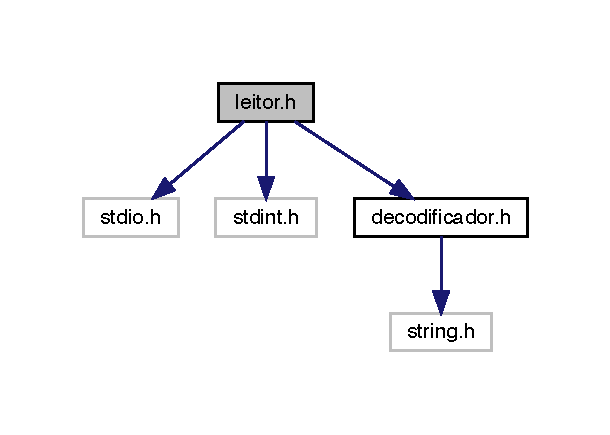
\includegraphics[width=293pt]{leitor_8h__incl}
\end{center}
\end{figure}
This graph shows which files directly or indirectly include this file\+:
\nopagebreak
\begin{figure}[H]
\begin{center}
\leavevmode
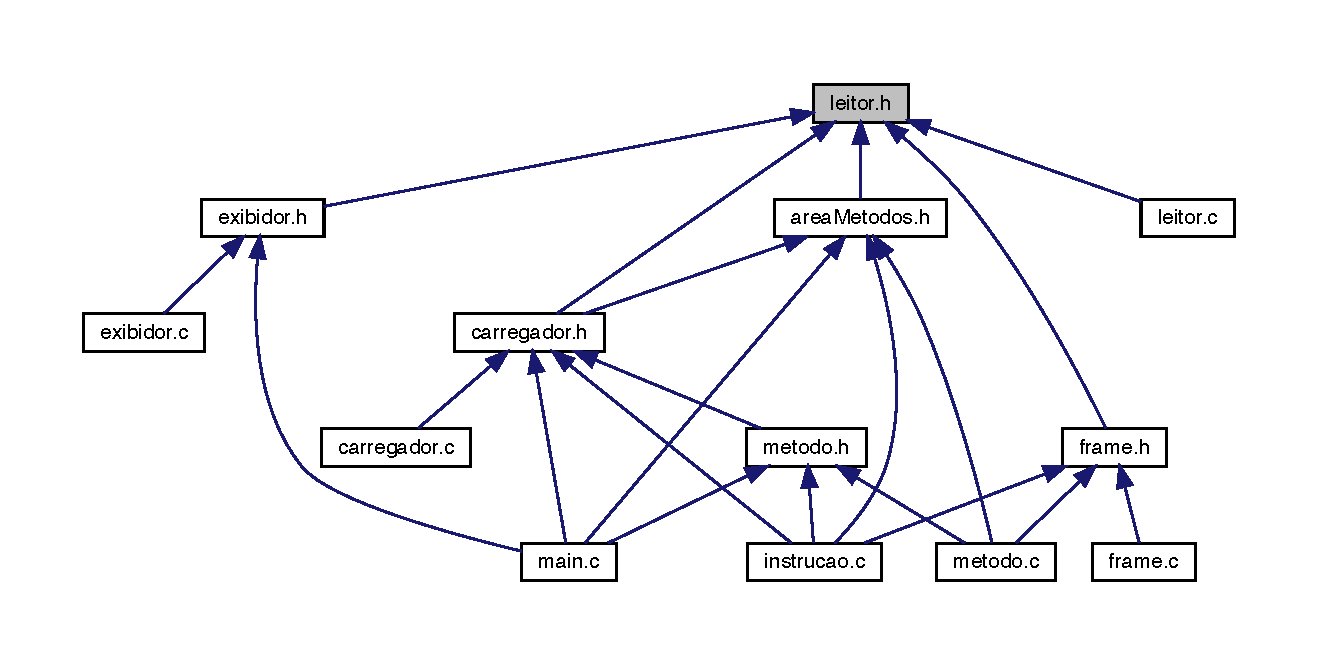
\includegraphics[width=350pt]{leitor_8h__dep__incl}
\end{center}
\end{figure}
\subsection*{Classes}
\begin{DoxyCompactItemize}
\item 
struct \mbox{\hyperlink{structCpInfo}{Cp\+Info}}
\begin{DoxyCompactList}\small\item\em A estrutura do cp\+\_\+info ira compor a constant\+\_\+pool do class\+File. \end{DoxyCompactList}\item 
struct \mbox{\hyperlink{structExceptionsAttribute}{Exceptions\+Attribute}}
\item 
struct \mbox{\hyperlink{structCvInfo}{Cv\+Info}}
\item 
struct \mbox{\hyperlink{structFieldInfo}{Field\+Info}}
\item 
struct \mbox{\hyperlink{structAttributeInfo}{Attribute\+Info}}
\item 
struct \mbox{\hyperlink{structExceptionTable}{Exception\+Table}}
\item 
struct \mbox{\hyperlink{structCodeAttribute}{Code\+Attribute}}
\item 
struct \mbox{\hyperlink{structMethodInfo}{Method\+Info}}
\item 
struct \mbox{\hyperlink{structClassFile}{Class\+File}}
\begin{DoxyCompactList}\small\item\em A estrutura de um class\+File em bytes (8-\/bits). \end{DoxyCompactList}\end{DoxyCompactItemize}
\subsection*{Macros}
\begin{DoxyCompactItemize}
\item 
\mbox{\Hypertarget{leitor_8h_a72b5b534aa409975da610a36f648fa0a}\label{leitor_8h_a72b5b534aa409975da610a36f648fa0a}} 
\#define \mbox{\hyperlink{leitor_8h_a72b5b534aa409975da610a36f648fa0a}{C\+O\+N\+S\+T\+A\+N\+T\+\_\+\+Class}}~7
\begin{DoxyCompactList}\small\item\em constante de Class definida como 7 \end{DoxyCompactList}\item 
\mbox{\Hypertarget{leitor_8h_a008d43478c2e2973e7413f5d1c48095d}\label{leitor_8h_a008d43478c2e2973e7413f5d1c48095d}} 
\#define \mbox{\hyperlink{leitor_8h_a008d43478c2e2973e7413f5d1c48095d}{C\+O\+N\+S\+T\+A\+N\+T\+\_\+\+Fieldref}}~9
\begin{DoxyCompactList}\small\item\em constante de Fieldref definida como 9 \end{DoxyCompactList}\item 
\mbox{\Hypertarget{leitor_8h_a2a179cf178ea867c6ab1700508c269dd}\label{leitor_8h_a2a179cf178ea867c6ab1700508c269dd}} 
\#define \mbox{\hyperlink{leitor_8h_a2a179cf178ea867c6ab1700508c269dd}{C\+O\+N\+S\+T\+A\+N\+T\+\_\+\+Methodref}}~10
\begin{DoxyCompactList}\small\item\em constante de Methodref definida como 10 \end{DoxyCompactList}\item 
\mbox{\Hypertarget{leitor_8h_ac0e92044d246c6e4d691116f89a70ebb}\label{leitor_8h_ac0e92044d246c6e4d691116f89a70ebb}} 
\#define \mbox{\hyperlink{leitor_8h_ac0e92044d246c6e4d691116f89a70ebb}{C\+O\+N\+S\+T\+A\+N\+T\+\_\+\+Interface\+Methodref}}~11
\begin{DoxyCompactList}\small\item\em constante de Interface\+Methodref definida como 11 \end{DoxyCompactList}\item 
\mbox{\Hypertarget{leitor_8h_a0a7acbe175de56072a2f0a1a051418e1}\label{leitor_8h_a0a7acbe175de56072a2f0a1a051418e1}} 
\#define \mbox{\hyperlink{leitor_8h_a0a7acbe175de56072a2f0a1a051418e1}{C\+O\+N\+S\+T\+A\+N\+T\+\_\+\+String}}~8
\begin{DoxyCompactList}\small\item\em constante de String como definida 8 \end{DoxyCompactList}\item 
\mbox{\Hypertarget{leitor_8h_a856a6553a55d721970ca5450eb1ccd2c}\label{leitor_8h_a856a6553a55d721970ca5450eb1ccd2c}} 
\#define \mbox{\hyperlink{leitor_8h_a856a6553a55d721970ca5450eb1ccd2c}{C\+O\+N\+S\+T\+A\+N\+T\+\_\+\+Integer}}~3
\begin{DoxyCompactList}\small\item\em constante de Integer definida como 3 \end{DoxyCompactList}\item 
\mbox{\Hypertarget{leitor_8h_ab914627ce5b25c4acfc98f2eacb78473}\label{leitor_8h_ab914627ce5b25c4acfc98f2eacb78473}} 
\#define \mbox{\hyperlink{leitor_8h_ab914627ce5b25c4acfc98f2eacb78473}{C\+O\+N\+S\+T\+A\+N\+T\+\_\+\+Float}}~4
\begin{DoxyCompactList}\small\item\em constante de Float definida como 4 \end{DoxyCompactList}\item 
\mbox{\Hypertarget{leitor_8h_a426ca017b895fc522671a561d460be7a}\label{leitor_8h_a426ca017b895fc522671a561d460be7a}} 
\#define \mbox{\hyperlink{leitor_8h_a426ca017b895fc522671a561d460be7a}{C\+O\+N\+S\+T\+A\+N\+T\+\_\+\+Long}}~5
\begin{DoxyCompactList}\small\item\em constante de Long definida como 5 \end{DoxyCompactList}\item 
\mbox{\Hypertarget{leitor_8h_ab49341c3b4ade4bfa1a64be8d2f73ae1}\label{leitor_8h_ab49341c3b4ade4bfa1a64be8d2f73ae1}} 
\#define \mbox{\hyperlink{leitor_8h_ab49341c3b4ade4bfa1a64be8d2f73ae1}{C\+O\+N\+S\+T\+A\+N\+T\+\_\+\+Double}}~6
\begin{DoxyCompactList}\small\item\em constante de Double definida como 6 \end{DoxyCompactList}\item 
\mbox{\Hypertarget{leitor_8h_a5b6ba749976ae61415983ca0b890c91a}\label{leitor_8h_a5b6ba749976ae61415983ca0b890c91a}} 
\#define \mbox{\hyperlink{leitor_8h_a5b6ba749976ae61415983ca0b890c91a}{C\+O\+N\+S\+T\+A\+N\+T\+\_\+\+Name\+And\+Type}}~12
\begin{DoxyCompactList}\small\item\em constante de Name\+And\+Type definida como 12 \end{DoxyCompactList}\item 
\mbox{\Hypertarget{leitor_8h_afc46559a7d3f7baf519fc183c2fad2b4}\label{leitor_8h_afc46559a7d3f7baf519fc183c2fad2b4}} 
\#define \mbox{\hyperlink{leitor_8h_afc46559a7d3f7baf519fc183c2fad2b4}{C\+O\+N\+S\+T\+A\+N\+T\+\_\+\+Utf8}}~1
\begin{DoxyCompactList}\small\item\em constante de Utf8 definida como 1 \end{DoxyCompactList}\item 
\mbox{\Hypertarget{leitor_8h_a4d34398b879119909a61e7f5d80d7f9a}\label{leitor_8h_a4d34398b879119909a61e7f5d80d7f9a}} 
\#define {\bfseries N\+U\+M\+\_\+\+I\+N\+S\+T\+R\+U\+C\+AO}~256
\item 
\mbox{\Hypertarget{leitor_8h_a1cdafd6c15f0fd29a71a55b339cf9de6}\label{leitor_8h_a1cdafd6c15f0fd29a71a55b339cf9de6}} 
\#define {\bfseries T\+A\+B\+L\+E\+S\+W\+I\+T\+CH}~170
\item 
\mbox{\Hypertarget{leitor_8h_a1687e8ea07fcbe04c58dc6f7a33d01eb}\label{leitor_8h_a1687e8ea07fcbe04c58dc6f7a33d01eb}} 
\#define {\bfseries L\+O\+O\+K\+U\+P\+S\+W\+I\+T\+CH}~171
\item 
\mbox{\Hypertarget{leitor_8h_aa88400ec102cd1e2e36de0eb301de232}\label{leitor_8h_aa88400ec102cd1e2e36de0eb301de232}} 
\#define {\bfseries W\+I\+DE}~196
\item 
\mbox{\Hypertarget{leitor_8h_a1330d3bc71feb429bab65632fdc76711}\label{leitor_8h_a1330d3bc71feb429bab65632fdc76711}} 
\#define {\bfseries B\+I\+P\+U\+SH}~16
\item 
\mbox{\Hypertarget{leitor_8h_af582412bbea0e7f8583b5f8a846b6026}\label{leitor_8h_af582412bbea0e7f8583b5f8a846b6026}} 
\#define {\bfseries S\+I\+P\+U\+SH}~16
\item 
\mbox{\Hypertarget{leitor_8h_a2c2adaf13d4f839e7e2e4a6b16606cd9}\label{leitor_8h_a2c2adaf13d4f839e7e2e4a6b16606cd9}} 
\#define {\bfseries L\+DC}~18
\item 
\mbox{\Hypertarget{leitor_8h_a98cbbc5f6d0e38792668336ef7e2bc6a}\label{leitor_8h_a98cbbc5f6d0e38792668336ef7e2bc6a}} 
\#define {\bfseries L\+D\+C\+\_\+W}~19
\item 
\mbox{\Hypertarget{leitor_8h_a17bc826fbbd05a4bd99cc1b9c1829254}\label{leitor_8h_a17bc826fbbd05a4bd99cc1b9c1829254}} 
\#define {\bfseries L\+D\+C2\+\_\+W}~20
\item 
\mbox{\Hypertarget{leitor_8h_ad5c77685edd36f34b11eeb25d2bea4ab}\label{leitor_8h_ad5c77685edd36f34b11eeb25d2bea4ab}} 
\#define {\bfseries I\+L\+O\+AD}~21
\item 
\mbox{\Hypertarget{leitor_8h_aa000af5bb4b3a1c5ff7279e73c76ac7e}\label{leitor_8h_aa000af5bb4b3a1c5ff7279e73c76ac7e}} 
\#define {\bfseries F\+L\+O\+AD}~23
\item 
\mbox{\Hypertarget{leitor_8h_a340dbcdfd6b5f22fc0cebdda08e69231}\label{leitor_8h_a340dbcdfd6b5f22fc0cebdda08e69231}} 
\#define {\bfseries A\+L\+O\+AD}~25
\item 
\mbox{\Hypertarget{leitor_8h_a885355811100d4454ef09c8713edfbad}\label{leitor_8h_a885355811100d4454ef09c8713edfbad}} 
\#define {\bfseries L\+L\+O\+AD}~22
\item 
\mbox{\Hypertarget{leitor_8h_ac264ddff2dda06da1706e895c7f12ed5}\label{leitor_8h_ac264ddff2dda06da1706e895c7f12ed5}} 
\#define {\bfseries D\+L\+O\+AD}~24
\item 
\mbox{\Hypertarget{leitor_8h_a0ea7a1a0d9ae1a4bc185116b8da3756f}\label{leitor_8h_a0ea7a1a0d9ae1a4bc185116b8da3756f}} 
\#define {\bfseries I\+S\+T\+O\+RE}~54
\item 
\mbox{\Hypertarget{leitor_8h_ae49a3b8c20d118590de89a05f2821a8e}\label{leitor_8h_ae49a3b8c20d118590de89a05f2821a8e}} 
\#define {\bfseries F\+S\+T\+O\+RE}~56
\item 
\mbox{\Hypertarget{leitor_8h_a1a56732b8344dbeca6c4cf19fda97e79}\label{leitor_8h_a1a56732b8344dbeca6c4cf19fda97e79}} 
\#define {\bfseries A\+S\+T\+O\+RE}~58
\item 
\mbox{\Hypertarget{leitor_8h_abdd7627850849525b29fc2aaa3d75986}\label{leitor_8h_abdd7627850849525b29fc2aaa3d75986}} 
\#define {\bfseries L\+S\+T\+O\+RE}~55
\item 
\mbox{\Hypertarget{leitor_8h_a2efaf68ebea2e64e13a99fd4bfd09303}\label{leitor_8h_a2efaf68ebea2e64e13a99fd4bfd09303}} 
\#define {\bfseries D\+S\+T\+O\+RE}~57
\item 
\mbox{\Hypertarget{leitor_8h_aa52eb3d830afe5ebd3684561942aeec9}\label{leitor_8h_aa52eb3d830afe5ebd3684561942aeec9}} 
\#define {\bfseries I\+I\+NC}~132
\item 
\mbox{\Hypertarget{leitor_8h_a8ffb94495a3f3a7562f6bd9a3e624a2b}\label{leitor_8h_a8ffb94495a3f3a7562f6bd9a3e624a2b}} 
\#define {\bfseries I\+F\+EQ}~153
\item 
\mbox{\Hypertarget{leitor_8h_a2a87011f85ff602bd4c93271824f48c5}\label{leitor_8h_a2a87011f85ff602bd4c93271824f48c5}} 
\#define {\bfseries I\+F\+NE}~154
\item 
\mbox{\Hypertarget{leitor_8h_abbc36648c78992026bea87a41408d3e0}\label{leitor_8h_abbc36648c78992026bea87a41408d3e0}} 
\#define {\bfseries I\+F\+LT}~155
\item 
\mbox{\Hypertarget{leitor_8h_a132c3c3bc734b725b37490c678533a2a}\label{leitor_8h_a132c3c3bc734b725b37490c678533a2a}} 
\#define {\bfseries I\+F\+GE}~156
\item 
\mbox{\Hypertarget{leitor_8h_a9d265e3e25f28c857e814b9f401fbea8}\label{leitor_8h_a9d265e3e25f28c857e814b9f401fbea8}} 
\#define {\bfseries I\+F\+GT}~157
\item 
\mbox{\Hypertarget{leitor_8h_a7911b2303014b118caf8ef9cbd7e0311}\label{leitor_8h_a7911b2303014b118caf8ef9cbd7e0311}} 
\#define {\bfseries I\+F\+LE}~158
\item 
\mbox{\Hypertarget{leitor_8h_abd5a8e8f905cac8348347e930d4e7d8a}\label{leitor_8h_abd5a8e8f905cac8348347e930d4e7d8a}} 
\#define {\bfseries I\+F\+\_\+\+I\+C\+M\+P\+EQ}~159
\item 
\mbox{\Hypertarget{leitor_8h_a8672d91981d5bd3ded069ea518964b86}\label{leitor_8h_a8672d91981d5bd3ded069ea518964b86}} 
\#define {\bfseries I\+F\+\_\+\+I\+C\+M\+P\+NE}~160
\item 
\mbox{\Hypertarget{leitor_8h_a5309bfc031f3eaf74f12f540acd38d73}\label{leitor_8h_a5309bfc031f3eaf74f12f540acd38d73}} 
\#define {\bfseries I\+F\+\_\+\+I\+C\+M\+P\+LT}~161
\item 
\mbox{\Hypertarget{leitor_8h_abe2a25387a2f2229624d22bd7bc8487e}\label{leitor_8h_abe2a25387a2f2229624d22bd7bc8487e}} 
\#define {\bfseries I\+F\+\_\+\+I\+C\+M\+P\+GE}~162
\item 
\mbox{\Hypertarget{leitor_8h_ad8d8274817a28ff4caef8d4790602e51}\label{leitor_8h_ad8d8274817a28ff4caef8d4790602e51}} 
\#define {\bfseries I\+F\+\_\+\+I\+C\+M\+P\+GT}~163
\item 
\mbox{\Hypertarget{leitor_8h_a96d5e11acb2e2783e9b268afc70b6db0}\label{leitor_8h_a96d5e11acb2e2783e9b268afc70b6db0}} 
\#define {\bfseries I\+F\+\_\+\+I\+C\+M\+P\+LE}~164
\item 
\mbox{\Hypertarget{leitor_8h_a33a5fa728bc85c3bfc55b2f0182ef7d2}\label{leitor_8h_a33a5fa728bc85c3bfc55b2f0182ef7d2}} 
\#define {\bfseries I\+F\+\_\+\+A\+C\+M\+P\+EQ}~165
\item 
\mbox{\Hypertarget{leitor_8h_aaf73f4576cb5b97ff22f316da952be9c}\label{leitor_8h_aaf73f4576cb5b97ff22f316da952be9c}} 
\#define {\bfseries I\+F\+\_\+\+A\+C\+M\+P\+NE}~166
\item 
\mbox{\Hypertarget{leitor_8h_a99c49863330dfa251ff4a631ba976dc7}\label{leitor_8h_a99c49863330dfa251ff4a631ba976dc7}} 
\#define {\bfseries G\+O\+TO}~167
\item 
\mbox{\Hypertarget{leitor_8h_ac2544c8b4fe3113b0d6bb62530692c21}\label{leitor_8h_ac2544c8b4fe3113b0d6bb62530692c21}} 
\#define {\bfseries R\+ET}~169
\item 
\mbox{\Hypertarget{leitor_8h_a61e733cf2b6a289803532b3c6b79ad4e}\label{leitor_8h_a61e733cf2b6a289803532b3c6b79ad4e}} 
\#define {\bfseries N\+E\+W\+A\+R\+R\+AY}~188
\item 
\mbox{\Hypertarget{leitor_8h_a8b491257f4700c74dee2e8222042a0bf}\label{leitor_8h_a8b491257f4700c74dee2e8222042a0bf}} 
\#define {\bfseries I\+F\+N\+U\+LL}~198
\item 
\mbox{\Hypertarget{leitor_8h_ae4a008625c8599410322ad704628ee30}\label{leitor_8h_ae4a008625c8599410322ad704628ee30}} 
\#define {\bfseries I\+F\+N\+O\+N\+N\+U\+LL}~199
\end{DoxyCompactItemize}
\subsection*{Typedefs}
\begin{DoxyCompactItemize}
\item 
typedef struct \mbox{\hyperlink{structCpInfo}{Cp\+Info}} \mbox{\hyperlink{leitor_8h_a6898bbbc40514b09ecea5a0aababd1be}{Cp\+Info}}
\begin{DoxyCompactList}\small\item\em A estrutura do cp\+\_\+info ira compor a constant\+\_\+pool do class\+File. \end{DoxyCompactList}\item 
\mbox{\Hypertarget{leitor_8h_a7abfd7cbf828c7d98811d0a4feae0ee6}\label{leitor_8h_a7abfd7cbf828c7d98811d0a4feae0ee6}} 
typedef struct \mbox{\hyperlink{structExceptionsAttribute}{Exceptions\+Attribute}} {\bfseries Exceptions\+Attribute}
\item 
\mbox{\Hypertarget{leitor_8h_a6b458e51f7e631d837bebc375806c99a}\label{leitor_8h_a6b458e51f7e631d837bebc375806c99a}} 
typedef struct \mbox{\hyperlink{structCvInfo}{Cv\+Info}} {\bfseries Cv\+Info}
\item 
\mbox{\Hypertarget{leitor_8h_aeb986aa95895f36df0534745f678466c}\label{leitor_8h_aeb986aa95895f36df0534745f678466c}} 
typedef struct \mbox{\hyperlink{structFieldInfo}{Field\+Info}} {\bfseries Field\+Info}
\item 
\mbox{\Hypertarget{leitor_8h_ae111dc3a7128bbe7b306f602c04eeaec}\label{leitor_8h_ae111dc3a7128bbe7b306f602c04eeaec}} 
typedef struct \mbox{\hyperlink{structAttributeInfo}{Attribute\+Info}} {\bfseries Attribute\+Info}
\item 
\mbox{\Hypertarget{leitor_8h_a24e796ea64f4e52720b89f3336ea5d90}\label{leitor_8h_a24e796ea64f4e52720b89f3336ea5d90}} 
typedef struct \mbox{\hyperlink{structExceptionTable}{Exception\+Table}} {\bfseries Exception\+Table}
\item 
\mbox{\Hypertarget{leitor_8h_a33a73fc4eb288c6fb10a53b37561e34d}\label{leitor_8h_a33a73fc4eb288c6fb10a53b37561e34d}} 
typedef struct \mbox{\hyperlink{structCodeAttribute}{Code\+Attribute}} {\bfseries Code\+Attribute}
\item 
\mbox{\Hypertarget{leitor_8h_a2b442a0842962df6623bfe654d11b7d3}\label{leitor_8h_a2b442a0842962df6623bfe654d11b7d3}} 
typedef struct \mbox{\hyperlink{structMethodInfo}{Method\+Info}} {\bfseries Method\+Info}
\item 
typedef struct \mbox{\hyperlink{structClassFile}{Class\+File}} \mbox{\hyperlink{leitor_8h_aa2722eac638126419cda16ab0a201376}{Class\+File}}
\begin{DoxyCompactList}\small\item\em A estrutura de um class\+File em bytes (8-\/bits). \end{DoxyCompactList}\end{DoxyCompactItemize}
\subsection*{Functions}
\begin{DoxyCompactItemize}
\item 
\mbox{\hyperlink{structClassFile}{Class\+File}} $\ast$ \mbox{\hyperlink{leitor_8h_a658f67ed6a3ca72248e7cc0eaba67ba5}{inicializa\+Leitor}} (char $\ast$)
\item 
void \mbox{\hyperlink{leitor_8h_a6c4f68e13e23b5765be0187a0cd1e1bf}{le\+Class\+File}} (F\+I\+LE $\ast$, \mbox{\hyperlink{structClassFile}{Class\+File}} $\ast$)
\item 
int \mbox{\hyperlink{leitor_8h_aa690fa269e79d6df38f509403e592e76}{cafe\+Babe\+Valido}} (F\+I\+LE $\ast$, \mbox{\hyperlink{structClassFile}{Class\+File}} $\ast$)
\item 
void \mbox{\hyperlink{leitor_8h_a9b40cc38171f10524e7b5ff37f67a2c2}{le\+Constant\+Pool}} (F\+I\+LE $\ast$, \mbox{\hyperlink{structClassFile}{Class\+File}} $\ast$)
\item 
void \mbox{\hyperlink{leitor_8h_a776579b8fdeab9f042ac52193a587269}{le\+Interface\+Info}} (F\+I\+LE $\ast$, \mbox{\hyperlink{structClassFile}{Class\+File}} $\ast$)
\item 
void \mbox{\hyperlink{leitor_8h_ac6b98a9881dc2cf0dfc83e3674129536}{le\+Field\+Info}} (F\+I\+LE $\ast$, \mbox{\hyperlink{structClassFile}{Class\+File}} $\ast$)
\item 
void \mbox{\hyperlink{leitor_8h_a65640b48b47bed299da6129adf80c472}{le\+Method\+Info}} (F\+I\+LE $\ast$, \mbox{\hyperlink{structClassFile}{Class\+File}} $\ast$)
\item 
void \mbox{\hyperlink{leitor_8h_a545e322073fac16d991309e76b56f075}{le\+Attribute\+Info}} (F\+I\+LE $\ast$, \mbox{\hyperlink{structClassFile}{Class\+File}} $\ast$)
\item 
void \mbox{\hyperlink{leitor_8h_ab959f4eb63ed8cea6502938660900e2b}{le\+Exc}} (F\+I\+LE $\ast$, \mbox{\hyperlink{structExceptionsAttribute}{Exceptions\+Attribute}} $\ast$$\ast$, uint16\+\_\+t, uint32\+\_\+t)
\item 
void \mbox{\hyperlink{leitor_8h_ad16fbcf0c0b1e099da4be9bade95d340}{le\+Code}} (F\+I\+LE $\ast$, \mbox{\hyperlink{structCodeAttribute}{Code\+Attribute}} $\ast$$\ast$, uint16\+\_\+t, uint32\+\_\+t)
\item 
uint8\+\_\+t \mbox{\hyperlink{leitor_8h_a47c4bbbfb7bd971781eecc01b3eac38b}{le1\+Byte}} (F\+I\+LE $\ast$)
\item 
uint16\+\_\+t \mbox{\hyperlink{leitor_8h_abcee6c2bbe126aedc6569ad14ec3cc5b}{le2\+Bytes}} (F\+I\+LE $\ast$)
\item 
uint32\+\_\+t \mbox{\hyperlink{leitor_8h_a22efb9a3b526751b6428b32993ba1485}{le4\+Bytes}} (F\+I\+LE $\ast$)
\item 
void \mbox{\hyperlink{leitor_8h_a801f483e0d6f965b0355a3f33ff68e70}{salva\+Instrucoes}} (F\+I\+LE $\ast$, \mbox{\hyperlink{structCodeAttribute}{Code\+Attribute}} $\ast$$\ast$)
\end{DoxyCompactItemize}


\subsection{Typedef Documentation}
\mbox{\Hypertarget{leitor_8h_aa2722eac638126419cda16ab0a201376}\label{leitor_8h_aa2722eac638126419cda16ab0a201376}} 
\index{leitor.h@{leitor.h}!ClassFile@{ClassFile}}
\index{ClassFile@{ClassFile}!leitor.h@{leitor.h}}
\subsubsection{\texorpdfstring{ClassFile}{ClassFile}}
{\footnotesize\ttfamily typedef struct \mbox{\hyperlink{structClassFile}{Class\+File}}  \mbox{\hyperlink{structClassFile}{Class\+File}}}



A estrutura de um class\+File em bytes (8-\/bits). 

A estrutura de um class\+File baseado em bytes de 8-\/bits. Todos os 16-\/bit, 32-\/bit, e 64-\/bit sao construidos por leituras de dois, quatro, e oito bytes (8bits) consecutivos. Dados de multibyte sao armazenados em ordem big-\/endian, onde o high-\/byte vem primeiro. \mbox{\Hypertarget{leitor_8h_a6898bbbc40514b09ecea5a0aababd1be}\label{leitor_8h_a6898bbbc40514b09ecea5a0aababd1be}} 
\index{leitor.h@{leitor.h}!CpInfo@{CpInfo}}
\index{CpInfo@{CpInfo}!leitor.h@{leitor.h}}
\subsubsection{\texorpdfstring{CpInfo}{CpInfo}}
{\footnotesize\ttfamily typedef struct \mbox{\hyperlink{structCpInfo}{Cp\+Info}}  \mbox{\hyperlink{structCpInfo}{Cp\+Info}}}



A estrutura do cp\+\_\+info ira compor a constant\+\_\+pool do class\+File. 

cp\+\_\+info varia de acordo com o byte lido em sua tag 

\subsection{Function Documentation}
\mbox{\Hypertarget{leitor_8h_aa690fa269e79d6df38f509403e592e76}\label{leitor_8h_aa690fa269e79d6df38f509403e592e76}} 
\index{leitor.h@{leitor.h}!cafeBabeValido@{cafeBabeValido}}
\index{cafeBabeValido@{cafeBabeValido}!leitor.h@{leitor.h}}
\subsubsection{\texorpdfstring{cafeBabeValido()}{cafeBabeValido()}}
{\footnotesize\ttfamily int cafe\+Babe\+Valido (\begin{DoxyParamCaption}\item[{F\+I\+LE $\ast$}]{fp,  }\item[{\mbox{\hyperlink{structClassFile}{Class\+File}} $\ast$}]{class\+File }\end{DoxyParamCaption})}

Funcao que avalia se o arquivo aberto eh de fato um classfile e se os bytes de control 0x\+C\+A\+F\+E\+B\+A\+BE estao corretamente no inicio do arquivo.


\begin{DoxyParams}{Parameters}
{\em F\+I\+L\+E$\ast$} & Descritor do arquivo .class que foi aberto para leitura \\
\hline
{\em Class\+File$\ast$} & Ponteiro para a estrutura Classi\+File \\
\hline
\end{DoxyParams}
\begin{DoxyReturn}{Returns}
{\ttfamily int} Resultado da verificacao (valor booleano) 
\end{DoxyReturn}
\begin{DoxySeeAlso}{See also}
\mbox{\hyperlink{leitor_8c_a69346e08c479223be1ec2294791b6d78}{le4\+Bytes}} 
\end{DoxySeeAlso}
\mbox{\Hypertarget{leitor_8h_a658f67ed6a3ca72248e7cc0eaba67ba5}\label{leitor_8h_a658f67ed6a3ca72248e7cc0eaba67ba5}} 
\index{leitor.h@{leitor.h}!inicializaLeitor@{inicializaLeitor}}
\index{inicializaLeitor@{inicializaLeitor}!leitor.h@{leitor.h}}
\subsubsection{\texorpdfstring{inicializaLeitor()}{inicializaLeitor()}}
{\footnotesize\ttfamily \mbox{\hyperlink{structClassFile}{Class\+File}}$\ast$ inicializa\+Leitor (\begin{DoxyParamCaption}\item[{char $\ast$}]{caminho\+Classe }\end{DoxyParamCaption})}

Funcao principal que comeca a leitura de um classfile.


\begin{DoxyParams}{Parameters}
{\em char$\ast$} & String com o caminho do arquivo .class a ser lido \\
\hline
\end{DoxyParams}
\begin{DoxyReturn}{Returns}
{\ttfamily Class\+File$\ast$} Uma estrutura \mbox{\hyperlink{structClassFile}{Class\+File}} preenchida 
\end{DoxyReturn}
\begin{DoxySeeAlso}{See also}
\mbox{\hyperlink{leitor_8c_a8a9afe01d56583162e5d2d4fba0a38aa}{le\+Class\+File}} 
\end{DoxySeeAlso}
\mbox{\Hypertarget{leitor_8h_a47c4bbbfb7bd971781eecc01b3eac38b}\label{leitor_8h_a47c4bbbfb7bd971781eecc01b3eac38b}} 
\index{leitor.h@{leitor.h}!le1Byte@{le1Byte}}
\index{le1Byte@{le1Byte}!leitor.h@{leitor.h}}
\subsubsection{\texorpdfstring{le1Byte()}{le1Byte()}}
{\footnotesize\ttfamily uint8\+\_\+t le1\+Byte (\begin{DoxyParamCaption}\item[{F\+I\+LE $\ast$}]{fp }\end{DoxyParamCaption})}

Funcao que le 1 byte e salva numa variavel unsigned de 8bits.


\begin{DoxyParams}{Parameters}
{\em F\+I\+L\+E$\ast$} & Descritor do arquivo .class que foi aberto para leitura \\
\hline
\end{DoxyParams}
\begin{DoxyReturn}{Returns}
{\ttfamily uint8\+\_\+t} O valor lido em um unsigned de 8bits 
\end{DoxyReturn}
\mbox{\Hypertarget{leitor_8h_abcee6c2bbe126aedc6569ad14ec3cc5b}\label{leitor_8h_abcee6c2bbe126aedc6569ad14ec3cc5b}} 
\index{leitor.h@{leitor.h}!le2Bytes@{le2Bytes}}
\index{le2Bytes@{le2Bytes}!leitor.h@{leitor.h}}
\subsubsection{\texorpdfstring{le2Bytes()}{le2Bytes()}}
{\footnotesize\ttfamily uint16\+\_\+t le2\+Bytes (\begin{DoxyParamCaption}\item[{F\+I\+LE $\ast$}]{fp }\end{DoxyParamCaption})}

Funcao que le 2 byte e salva numa variavel unsigned de 16bits.


\begin{DoxyParams}{Parameters}
{\em F\+I\+L\+E$\ast$} & Descritor do arquivo .class que foi aberto para leitura \\
\hline
\end{DoxyParams}
\begin{DoxyReturn}{Returns}
{\ttfamily uint16\+\_\+t} O valor lido em um unsigned de 16bits 
\end{DoxyReturn}
\mbox{\Hypertarget{leitor_8h_a22efb9a3b526751b6428b32993ba1485}\label{leitor_8h_a22efb9a3b526751b6428b32993ba1485}} 
\index{leitor.h@{leitor.h}!le4Bytes@{le4Bytes}}
\index{le4Bytes@{le4Bytes}!leitor.h@{leitor.h}}
\subsubsection{\texorpdfstring{le4Bytes()}{le4Bytes()}}
{\footnotesize\ttfamily uint32\+\_\+t le4\+Bytes (\begin{DoxyParamCaption}\item[{F\+I\+LE $\ast$}]{fp }\end{DoxyParamCaption})}

Funcao que le 4 byte e salva numa variavel unsigned de 32bits.


\begin{DoxyParams}{Parameters}
{\em F\+I\+L\+E$\ast$} & Descritor do arquivo .class que foi aberto para leitura \\
\hline
\end{DoxyParams}
\begin{DoxyReturn}{Returns}
{\ttfamily uint32\+\_\+t} O valor lido em um unsigned de 32bits 
\end{DoxyReturn}
\mbox{\Hypertarget{leitor_8h_a545e322073fac16d991309e76b56f075}\label{leitor_8h_a545e322073fac16d991309e76b56f075}} 
\index{leitor.h@{leitor.h}!leAttributeInfo@{leAttributeInfo}}
\index{leAttributeInfo@{leAttributeInfo}!leitor.h@{leitor.h}}
\subsubsection{\texorpdfstring{leAttributeInfo()}{leAttributeInfo()}}
{\footnotesize\ttfamily void le\+Attribute\+Info (\begin{DoxyParamCaption}\item[{F\+I\+LE $\ast$}]{fp,  }\item[{\mbox{\hyperlink{structClassFile}{Class\+File}} $\ast$}]{class\+File }\end{DoxyParamCaption})}

Funcao que le os bytes que compoe as Informacoes de Atributos e os armazena nas devidas posicoes da estrutura \mbox{\hyperlink{structAttributeInfo}{Attribute\+Info}}, dentro do \mbox{\hyperlink{structClassFile}{Class\+File}} recebido como parametro.


\begin{DoxyParams}{Parameters}
{\em F\+I\+L\+E$\ast$} & Descritor do arquivo .class que foi aberto para leitura \\
\hline
{\em Class\+File$\ast$} & Ponteiro para a estrutura Classi\+File \\
\hline
\end{DoxyParams}
\begin{DoxyReturn}{Returns}
{\ttfamily void} 
\end{DoxyReturn}
\begin{DoxySeeAlso}{See also}
\mbox{\hyperlink{leitor_8c_a90fdde4380531bf81ba1284254004eff}{le2\+Bytes}} \mbox{\hyperlink{leitor_8c_a69346e08c479223be1ec2294791b6d78}{le4\+Bytes}} 
\end{DoxySeeAlso}
\mbox{\Hypertarget{leitor_8h_a6c4f68e13e23b5765be0187a0cd1e1bf}\label{leitor_8h_a6c4f68e13e23b5765be0187a0cd1e1bf}} 
\index{leitor.h@{leitor.h}!leClassFile@{leClassFile}}
\index{leClassFile@{leClassFile}!leitor.h@{leitor.h}}
\subsubsection{\texorpdfstring{leClassFile()}{leClassFile()}}
{\footnotesize\ttfamily void le\+Class\+File (\begin{DoxyParamCaption}\item[{F\+I\+LE $\ast$}]{fp,  }\item[{\mbox{\hyperlink{structClassFile}{Class\+File}} $\ast$}]{class\+File }\end{DoxyParamCaption})}

Funcao que coordena a leitura do arquivo .class e coordena as chamadas das funcoes que leem cada parte do classfile individualmente e preenchem a estrutura recebida como parametro.


\begin{DoxyParams}{Parameters}
{\em F\+I\+L\+E$\ast$} & Descritor do arquivo .class que foi aberto para leitura \\
\hline
{\em Class\+File$\ast$} & Ponteiro para a estrutura Classi\+File vazia (porem ja alocada) \\
\hline
\end{DoxyParams}
\begin{DoxyReturn}{Returns}
{\ttfamily void} 
\end{DoxyReturn}
\begin{DoxySeeAlso}{See also}
\mbox{\hyperlink{leitor_8c_a878e3123a0ef2433fba5355ceba54703}{cafe\+Babe\+Valido}} \mbox{\hyperlink{leitor_8c_a90fdde4380531bf81ba1284254004eff}{le2\+Bytes}} \mbox{\hyperlink{leitor_8c_a52487a1b0952e0c2f4bc22db6ac53153}{le\+Constant\+Pool}} \mbox{\hyperlink{leitor_8c_abf67c5dca9a8c23f380c37fa95c9c215}{le\+Interface\+Info}} \mbox{\hyperlink{leitor_8c_a99d0519fab7e0cd8b33a6451649e3d22}{le\+Field\+Info}} \mbox{\hyperlink{leitor_8c_a6d4e3deddb19180bc91b1892a5f8cc28}{le\+Method\+Info}} \mbox{\hyperlink{leitor_8c_adac81aedb40c82f25e42a66979a28d86}{le\+Attribute\+Info}} 
\end{DoxySeeAlso}
\mbox{\Hypertarget{leitor_8h_ad16fbcf0c0b1e099da4be9bade95d340}\label{leitor_8h_ad16fbcf0c0b1e099da4be9bade95d340}} 
\index{leitor.h@{leitor.h}!leCode@{leCode}}
\index{leCode@{leCode}!leitor.h@{leitor.h}}
\subsubsection{\texorpdfstring{leCode()}{leCode()}}
{\footnotesize\ttfamily void le\+Code (\begin{DoxyParamCaption}\item[{F\+I\+LE $\ast$}]{fp,  }\item[{\mbox{\hyperlink{structCodeAttribute}{Code\+Attribute}} $\ast$$\ast$}]{cd\+Atrb,  }\item[{uint16\+\_\+t}]{name\+Index,  }\item[{uint32\+\_\+t}]{attributes\+Count }\end{DoxyParamCaption})}

Funcao que le o codigo (mnemonicos) de um metodo e os armazena nas devidas posicoes da estrutura \mbox{\hyperlink{structCodeAttribute}{Code\+Attribute}}.


\begin{DoxyParams}{Parameters}
{\em F\+I\+L\+E$\ast$} & Descritor do arquivo .class que foi aberto para leitura \\
\hline
{\em Code\+Attribute$\ast$$\ast$} & Ponteiro para uma estrutura \mbox{\hyperlink{structCodeAttribute}{Code\+Attribute}} \\
\hline
{\em uint16\+\_\+t} & Name\+Index do metodo cujas instrucoes serao lidas \\
\hline
{\em uint16\+\_\+t} & Quantidade de atributos do metodo \\
\hline
\end{DoxyParams}
\begin{DoxyReturn}{Returns}
{\ttfamily void} 
\end{DoxyReturn}
\begin{DoxySeeAlso}{See also}
\mbox{\hyperlink{leitor_8c_a2ef408b96bee8729ac29bf490229048f}{le1\+Byte}} \mbox{\hyperlink{leitor_8c_a90fdde4380531bf81ba1284254004eff}{le2\+Bytes}} \mbox{\hyperlink{leitor_8c_a69346e08c479223be1ec2294791b6d78}{le4\+Bytes}} \mbox{\hyperlink{leitor_8c_ab80e6e4a3faed37485e9411ddfc3e549}{salva\+Instrucoes}} 
\end{DoxySeeAlso}
\mbox{\Hypertarget{leitor_8h_a9b40cc38171f10524e7b5ff37f67a2c2}\label{leitor_8h_a9b40cc38171f10524e7b5ff37f67a2c2}} 
\index{leitor.h@{leitor.h}!leConstantPool@{leConstantPool}}
\index{leConstantPool@{leConstantPool}!leitor.h@{leitor.h}}
\subsubsection{\texorpdfstring{leConstantPool()}{leConstantPool()}}
{\footnotesize\ttfamily void le\+Constant\+Pool (\begin{DoxyParamCaption}\item[{F\+I\+LE $\ast$}]{fp,  }\item[{\mbox{\hyperlink{structClassFile}{Class\+File}} $\ast$}]{class\+File }\end{DoxyParamCaption})}

Funcao que le os bytes que compoe o Constant Pool e os armazena nas devidas posicoes da estrutura \mbox{\hyperlink{structCpInfo}{Cp\+Info}}, dentro do \mbox{\hyperlink{structClassFile}{Class\+File}} recebido como parametro.


\begin{DoxyParams}{Parameters}
{\em F\+I\+L\+E$\ast$} & Descritor do arquivo .class que foi aberto para leitura \\
\hline
{\em Class\+File$\ast$} & Ponteiro para a estrutura Classi\+File \\
\hline
\end{DoxyParams}
\begin{DoxyReturn}{Returns}
{\ttfamily void} 
\end{DoxyReturn}
\begin{DoxySeeAlso}{See also}
\mbox{\hyperlink{leitor_8c_a2ef408b96bee8729ac29bf490229048f}{le1\+Byte}} \mbox{\hyperlink{leitor_8c_a90fdde4380531bf81ba1284254004eff}{le2\+Bytes}} \mbox{\hyperlink{leitor_8c_a69346e08c479223be1ec2294791b6d78}{le4\+Bytes}} 
\end{DoxySeeAlso}
\mbox{\Hypertarget{leitor_8h_ab959f4eb63ed8cea6502938660900e2b}\label{leitor_8h_ab959f4eb63ed8cea6502938660900e2b}} 
\index{leitor.h@{leitor.h}!leExc@{leExc}}
\index{leExc@{leExc}!leitor.h@{leitor.h}}
\subsubsection{\texorpdfstring{leExc()}{leExc()}}
{\footnotesize\ttfamily void le\+Exc (\begin{DoxyParamCaption}\item[{F\+I\+LE $\ast$}]{fp,  }\item[{\mbox{\hyperlink{structExceptionsAttribute}{Exceptions\+Attribute}} $\ast$$\ast$}]{exc\+Atrb,  }\item[{uint16\+\_\+t}]{name\+Index,  }\item[{uint32\+\_\+t}]{attributes\+Count }\end{DoxyParamCaption})}

Funcao que le as excecoes (quando definidas) de um metodo da classe e os armazena nas devidas posicoes da estrutura \mbox{\hyperlink{structExceptionsAttribute}{Exceptions\+Attribute}}.


\begin{DoxyParams}{Parameters}
{\em F\+I\+L\+E$\ast$} & Descritor do arquivo .class que foi aberto para leitura \\
\hline
{\em Exceptions\+Attribute$\ast$$\ast$} & Ponteiro para uma estrutura \mbox{\hyperlink{structExceptionsAttribute}{Exceptions\+Attribute}} \\
\hline
{\em uint16\+\_\+t} & Name\+Index do metodo cujas excecoes serao lidas \\
\hline
{\em uint16\+\_\+t} & Quantidade de atributos do metodo \\
\hline
\end{DoxyParams}
\begin{DoxyReturn}{Returns}
{\ttfamily void} 
\end{DoxyReturn}
\begin{DoxySeeAlso}{See also}
\mbox{\hyperlink{leitor_8c_a90fdde4380531bf81ba1284254004eff}{le2\+Bytes}} 
\end{DoxySeeAlso}
\mbox{\Hypertarget{leitor_8h_ac6b98a9881dc2cf0dfc83e3674129536}\label{leitor_8h_ac6b98a9881dc2cf0dfc83e3674129536}} 
\index{leitor.h@{leitor.h}!leFieldInfo@{leFieldInfo}}
\index{leFieldInfo@{leFieldInfo}!leitor.h@{leitor.h}}
\subsubsection{\texorpdfstring{leFieldInfo()}{leFieldInfo()}}
{\footnotesize\ttfamily void le\+Field\+Info (\begin{DoxyParamCaption}\item[{F\+I\+LE $\ast$}]{fp,  }\item[{\mbox{\hyperlink{structClassFile}{Class\+File}} $\ast$}]{class\+File }\end{DoxyParamCaption})}

Funcao que le os bytes que compoe as Informacoes de Fields e os armazena nas devidas posicoes da estrutura \mbox{\hyperlink{structFieldInfo}{Field\+Info}}, dentro do \mbox{\hyperlink{structClassFile}{Class\+File}} recebido como parametro.


\begin{DoxyParams}{Parameters}
{\em F\+I\+L\+E$\ast$} & Descritor do arquivo .class que foi aberto para leitura \\
\hline
{\em Class\+File$\ast$} & Ponteiro para a estrutura Classi\+File \\
\hline
\end{DoxyParams}
\begin{DoxyReturn}{Returns}
{\ttfamily void} 
\end{DoxyReturn}
\begin{DoxySeeAlso}{See also}
\mbox{\hyperlink{leitor_8c_a90fdde4380531bf81ba1284254004eff}{le2\+Bytes}} \mbox{\hyperlink{leitor_8c_a69346e08c479223be1ec2294791b6d78}{le4\+Bytes}} 
\end{DoxySeeAlso}
\mbox{\Hypertarget{leitor_8h_a776579b8fdeab9f042ac52193a587269}\label{leitor_8h_a776579b8fdeab9f042ac52193a587269}} 
\index{leitor.h@{leitor.h}!leInterfaceInfo@{leInterfaceInfo}}
\index{leInterfaceInfo@{leInterfaceInfo}!leitor.h@{leitor.h}}
\subsubsection{\texorpdfstring{leInterfaceInfo()}{leInterfaceInfo()}}
{\footnotesize\ttfamily void le\+Interface\+Info (\begin{DoxyParamCaption}\item[{F\+I\+LE $\ast$}]{fp,  }\item[{\mbox{\hyperlink{structClassFile}{Class\+File}} $\ast$}]{class\+File }\end{DoxyParamCaption})}

Funcao que le os bytes que compoe as Informacoes de Interface e os armazena nas devidas posicoes da estrutura Interface\+Info, dentro do \mbox{\hyperlink{structClassFile}{Class\+File}} recebido como parametro.


\begin{DoxyParams}{Parameters}
{\em F\+I\+L\+E$\ast$} & Descritor do arquivo .class que foi aberto para leitura \\
\hline
{\em Class\+File$\ast$} & Ponteiro para a estrutura Classi\+File \\
\hline
\end{DoxyParams}
\begin{DoxyReturn}{Returns}
{\ttfamily void} 
\end{DoxyReturn}
\begin{DoxySeeAlso}{See also}
\mbox{\hyperlink{leitor_8c_a90fdde4380531bf81ba1284254004eff}{le2\+Bytes}} 
\end{DoxySeeAlso}
\mbox{\Hypertarget{leitor_8h_a65640b48b47bed299da6129adf80c472}\label{leitor_8h_a65640b48b47bed299da6129adf80c472}} 
\index{leitor.h@{leitor.h}!leMethodInfo@{leMethodInfo}}
\index{leMethodInfo@{leMethodInfo}!leitor.h@{leitor.h}}
\subsubsection{\texorpdfstring{leMethodInfo()}{leMethodInfo()}}
{\footnotesize\ttfamily void le\+Method\+Info (\begin{DoxyParamCaption}\item[{F\+I\+LE $\ast$}]{fp,  }\item[{\mbox{\hyperlink{structClassFile}{Class\+File}} $\ast$}]{class\+File }\end{DoxyParamCaption})}

Funcao que le os bytes que compoe as Informacoes de Metodos e os armazena nas devidas posicoes da estrutura \mbox{\hyperlink{structMethodInfo}{Method\+Info}}, dentro do \mbox{\hyperlink{structClassFile}{Class\+File}} recebido como parametro. Isso tudo incluindo codigo (instrucoes) e excecoes de cada metodo.


\begin{DoxyParams}{Parameters}
{\em F\+I\+L\+E$\ast$} & Descritor do arquivo .class que foi aberto para leitura \\
\hline
{\em Class\+File$\ast$} & Ponteiro para a estrutura Classi\+File \\
\hline
\end{DoxyParams}
\begin{DoxyReturn}{Returns}
{\ttfamily void} 
\end{DoxyReturn}
\begin{DoxySeeAlso}{See also}
\mbox{\hyperlink{leitor_8c_a2ef408b96bee8729ac29bf490229048f}{le1\+Byte}} \mbox{\hyperlink{leitor_8c_a90fdde4380531bf81ba1284254004eff}{le2\+Bytes}} \mbox{\hyperlink{leitor_8c_a69346e08c479223be1ec2294791b6d78}{le4\+Bytes}} \mbox{\hyperlink{leitor_8c_a6d55676267e5cf93c52566d78e1d11e1}{le\+Code}} \mbox{\hyperlink{leitor_8c_a9eb52b74df81ab0e0da46175d591d81f}{le\+Exc}} 
\end{DoxySeeAlso}
\mbox{\Hypertarget{leitor_8h_a801f483e0d6f965b0355a3f33ff68e70}\label{leitor_8h_a801f483e0d6f965b0355a3f33ff68e70}} 
\index{leitor.h@{leitor.h}!salvaInstrucoes@{salvaInstrucoes}}
\index{salvaInstrucoes@{salvaInstrucoes}!leitor.h@{leitor.h}}
\subsubsection{\texorpdfstring{salvaInstrucoes()}{salvaInstrucoes()}}
{\footnotesize\ttfamily void salva\+Instrucoes (\begin{DoxyParamCaption}\item[{F\+I\+LE $\ast$}]{fp,  }\item[{\mbox{\hyperlink{structCodeAttribute}{Code\+Attribute}} $\ast$$\ast$}]{cd\+Atrb }\end{DoxyParamCaption})}

Funcao que traduz os bytes de codigo lidos de um metodo e os armazena nas devidas posicoes da estrutura \mbox{\hyperlink{structCodeAttribute}{Code\+Attribute}}.


\begin{DoxyParams}{Parameters}
{\em F\+I\+L\+E$\ast$} & Descritor do arquivo .class que foi aberto para leitura \\
\hline
{\em Code\+Attribute$\ast$$\ast$} & Ponteiro para uma estrutura \mbox{\hyperlink{structCodeAttribute}{Code\+Attribute}} \\
\hline
\end{DoxyParams}
\begin{DoxyReturn}{Returns}
{\ttfamily void} 
\end{DoxyReturn}
\begin{DoxySeeAlso}{See also}
\mbox{\hyperlink{decodificador_8h_a33a5a572beb55160cd59df462a10cdc3}{inicializa\+Decodificador}} 
\end{DoxySeeAlso}

\hypertarget{main_8c}{}\section{main.\+c File Reference}
\label{main_8c}\index{main.c@{main.c}}


Arquivo principal que inicia a execucacao da J\+VM.  


{\ttfamily \#include \char`\"{}carregador.\+h\char`\"{}}\newline
{\ttfamily \#include \char`\"{}metodo.\+h\char`\"{}}\newline
{\ttfamily \#include \char`\"{}area\+Metodos.\+h\char`\"{}}\newline
{\ttfamily \#include \char`\"{}exibidor.\+h\char`\"{}}\newline
{\ttfamily \#include $<$stdio.\+h$>$}\newline
{\ttfamily \#include $<$stdlib.\+h$>$}\newline
Include dependency graph for main.\+c\+:
\nopagebreak
\begin{figure}[H]
\begin{center}
\leavevmode
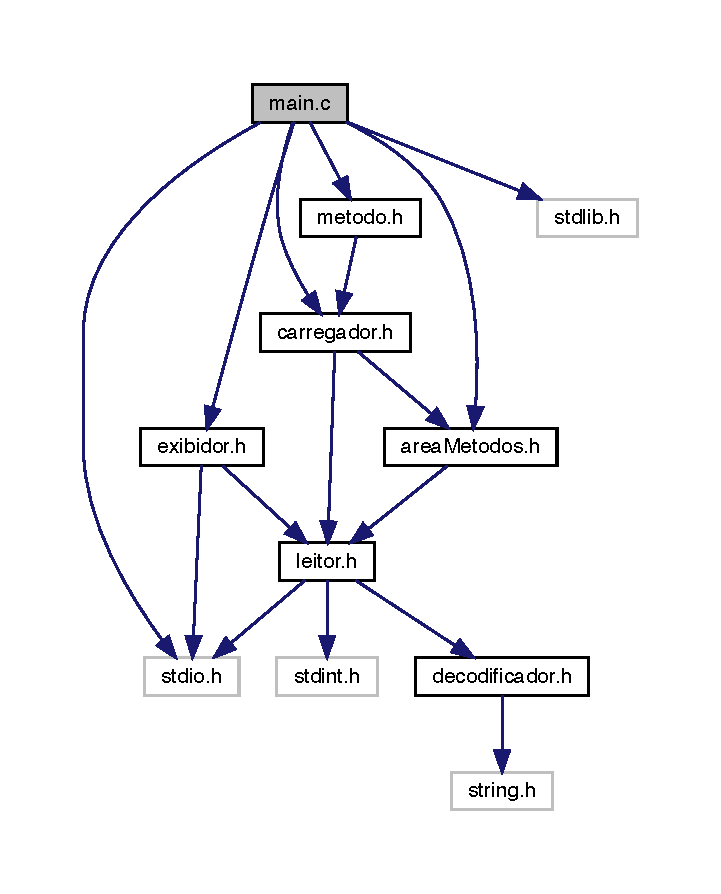
\includegraphics[width=346pt]{main_8c__incl}
\end{center}
\end{figure}
\subsection*{Macros}
\begin{DoxyCompactItemize}
\item 
\mbox{\Hypertarget{main_8c_a7b786c529b0d8bfcde5f815492e84db9}\label{main_8c_a7b786c529b0d8bfcde5f815492e84db9}} 
\#define {\bfseries T\+A\+M\+A\+N\+H\+O\+\_\+\+A\+R\+Q\+U\+I\+VO}~100
\end{DoxyCompactItemize}
\subsection*{Functions}
\begin{DoxyCompactItemize}
\item 
\mbox{\Hypertarget{main_8c_a45b099240a0e5e7ffff39bfa8accaf25}\label{main_8c_a45b099240a0e5e7ffff39bfa8accaf25}} 
void {\bfseries le\+Params\+Entrada} ()
\item 
void \mbox{\hyperlink{main_8c_a6b2cbabf8682bcc1712ff9adf23cecc7}{prepara\+Metodo\+Main}} ()
\item 
void \mbox{\hyperlink{main_8c_a4fb190a31887509a84011fe503d1583c}{exibe\+Array\+Classes}} ()
\item 
int \mbox{\hyperlink{main_8c_a0ddf1224851353fc92bfbff6f499fa97}{main}} (int argc, char $\ast$argv\mbox{[}$\,$\mbox{]})
\item 
void \mbox{\hyperlink{main_8c_aac9775bae25ad3825c28d3b01e78033c}{le\+Params\+Entrada}} (int argc, char $\ast$argv\mbox{[}$\,$\mbox{]})
\end{DoxyCompactItemize}
\subsection*{Variables}
\begin{DoxyCompactItemize}
\item 
\mbox{\Hypertarget{main_8c_a748d925b1fa9d6526aa5a94080aeaf19}\label{main_8c_a748d925b1fa9d6526aa5a94080aeaf19}} 
\mbox{\hyperlink{structMethodInfo}{Method\+Info}} $\ast$ {\bfseries metodo\+Main}
\item 
\mbox{\Hypertarget{main_8c_a5eb03fa1550ef172a859dba26a46d77a}\label{main_8c_a5eb03fa1550ef172a859dba26a46d77a}} 
\mbox{\hyperlink{structClassFile}{Class\+File}} $\ast$ {\bfseries classe\+Main}
\item 
\mbox{\Hypertarget{main_8c_a69c926fdbe16a1cbc50de4a966d497a5}\label{main_8c_a69c926fdbe16a1cbc50de4a966d497a5}} 
char $\ast$ {\bfseries caminho\+Arquivo}
\item 
\mbox{\Hypertarget{main_8c_a674404696468f40cd7392da3d3c502d7}\label{main_8c_a674404696468f40cd7392da3d3c502d7}} 
int {\bfseries exibe\+Class\+File}
\end{DoxyCompactItemize}


\subsection{Detailed Description}
Arquivo principal que inicia a execucacao da J\+VM. 

\begin{DoxyAuthor}{Authors}
Bruno Sanguinetti 18/0046063 ~\newline
Gabriel Vasconcelos 16/0120781 ~\newline
Leonardo de Almeida 15/0135491 ~\newline
Lucas Mafra 12/0126443 ~\newline
Wladimir Gramacho 15/0058718 ~\newline
 
\end{DoxyAuthor}
\begin{DoxyDate}{Date}
28/06/2019
\end{DoxyDate}
Inicializa o programa, pegando o caminho do arquivo \char`\"{}.\+class\char`\"{} e uma flag para impressao na tela. Ambos por por linha de comando, ou por interface. Entao, chama o Carregador para processar o arquivo e carregar a area de metodos (\mbox{\hyperlink{structAreaMetodos}{Area\+Metodos}}) para a memoria. Entao, comeca a execucaco do metodo main da classe principal e encerra quando a pilha de frames estiver vazia, imprimindo as estruturas na tela (caso o usuario tenha solicitado). 

\subsection{Function Documentation}
\mbox{\Hypertarget{main_8c_a4fb190a31887509a84011fe503d1583c}\label{main_8c_a4fb190a31887509a84011fe503d1583c}} 
\index{main.c@{main.c}!exibeArrayClasses@{exibeArrayClasses}}
\index{exibeArrayClasses@{exibeArrayClasses}!main.c@{main.c}}
\subsubsection{\texorpdfstring{exibeArrayClasses()}{exibeArrayClasses()}}
{\footnotesize\ttfamily void exibe\+Array\+Classes (\begin{DoxyParamCaption}{ }\end{DoxyParamCaption})}

Mostra o bytecode da classe lida no terminal e criar um arquivo de texto \char`\"{}log.\+txt\char`\"{} com o bytecode da classe caso a flag printa\+Para\+Arquivo tenha sido setada.


\begin{DoxyParams}{Parameters}
{\em Nao} & possui paramentros \\
\hline
\end{DoxyParams}
\begin{DoxyReturn}{Returns}
{\ttfamily void} 
\end{DoxyReturn}
\begin{DoxySeeAlso}{See also}
\mbox{\hyperlink{exibidor_8h_a157efd9bd041a04a6a6445a4fb44f3fb}{printa\+Class\+File}} 
\end{DoxySeeAlso}
\mbox{\Hypertarget{main_8c_aac9775bae25ad3825c28d3b01e78033c}\label{main_8c_aac9775bae25ad3825c28d3b01e78033c}} 
\index{main.c@{main.c}!leParamsEntrada@{leParamsEntrada}}
\index{leParamsEntrada@{leParamsEntrada}!main.c@{main.c}}
\subsubsection{\texorpdfstring{leParamsEntrada()}{leParamsEntrada()}}
{\footnotesize\ttfamily void le\+Params\+Entrada (\begin{DoxyParamCaption}\item[{int}]{argc,  }\item[{char $\ast$}]{argv\mbox{[}$\,$\mbox{]} }\end{DoxyParamCaption})}

Le os paramentros inseridos via linha de comando.


\begin{DoxyParams}{Parameters}
{\em int} & Numero de argumentos passados por command line \\
\hline
{\em char$\ast$} & Array que contem as strings passadas por command line \\
\hline
\end{DoxyParams}
\begin{DoxyReturn}{Returns}
{\ttfamily void} 
\end{DoxyReturn}
\mbox{\Hypertarget{main_8c_a0ddf1224851353fc92bfbff6f499fa97}\label{main_8c_a0ddf1224851353fc92bfbff6f499fa97}} 
\index{main.c@{main.c}!main@{main}}
\index{main@{main}!main.c@{main.c}}
\subsubsection{\texorpdfstring{main()}{main()}}
{\footnotesize\ttfamily int main (\begin{DoxyParamCaption}\item[{int}]{argc,  }\item[{char $\ast$}]{argv\mbox{[}$\,$\mbox{]} }\end{DoxyParamCaption})}

Main function da J\+VM -\/ Chama as funções de leitura de parametros, carregamento. para memoria, exibição do class file (se ativo por flag) normalização de metodo, empilhar método, executar frame e liberar memoria 
\begin{DoxyParams}{Parameters}
{\em int} & Numero de argumentos passados por command line \\
\hline
{\em char$\ast$} & Vetor que contem as strings passador por command line \\
\hline
\end{DoxyParams}
\begin{DoxyReturn}{Returns}
{\ttfamily int} Retorna 0 caso a execucao seja bem sucedida. 
\end{DoxyReturn}
\begin{DoxySeeAlso}{See also}
\mbox{\hyperlink{main_8c_aac9775bae25ad3825c28d3b01e78033c}{le\+Params\+Entrada}} \mbox{\hyperlink{carregador_8h_a6be3551b88a5154690e9e147217ca181}{carrega\+Classe\+Para\+Memoria}} \mbox{\hyperlink{main_8c_a6b2cbabf8682bcc1712ff9adf23cecc7}{prepara\+Metodo\+Main}} \mbox{\hyperlink{metodo_8h_a68acc5b3f2238f62b7d0ee50964183c1}{empilha\+Metodo}} \mbox{\hyperlink{metodo_8h_ae6a6b8342dd5977b74379e5295614ea8}{executa\+Frame\+Corrente}} \mbox{\hyperlink{main_8c_a4fb190a31887509a84011fe503d1583c}{exibe\+Array\+Classes}} 
\end{DoxySeeAlso}
\mbox{\Hypertarget{main_8c_a6b2cbabf8682bcc1712ff9adf23cecc7}\label{main_8c_a6b2cbabf8682bcc1712ff9adf23cecc7}} 
\index{main.c@{main.c}!preparaMetodoMain@{preparaMetodoMain}}
\index{preparaMetodoMain@{preparaMetodoMain}!main.c@{main.c}}
\subsubsection{\texorpdfstring{preparaMetodoMain()}{preparaMetodoMain()}}
{\footnotesize\ttfamily void prepara\+Metodo\+Main (\begin{DoxyParamCaption}{ }\end{DoxyParamCaption})}

Busca a classe que possui o metodo main e depois busca dentro dessa classe o metodo main.


\begin{DoxyParams}{Parameters}
{\em Nenhum} & \\
\hline
\end{DoxyParams}
\begin{DoxyReturn}{Returns}
{\ttfamily void} 
\end{DoxyReturn}
\begin{DoxySeeAlso}{See also}
\mbox{\hyperlink{carregador_8h_a5e44435bd5cfcea055179495059b1b2d}{busca\+Class\+Por\+Indice}} \mbox{\hyperlink{metodo_8c_a6aa5c3f94b9def67427ad40fb5205c5f}{busca\+Metodo\+Main}} 
\end{DoxySeeAlso}

\hypertarget{metodo_8c}{}\section{metodo.\+c File Reference}
\label{metodo_8c}\index{metodo.\+c@{metodo.\+c}}


Arquivo que carrega a area de metodos na memoria para inciar a execucao do programa Java.  


{\ttfamily \#include \char`\"{}frame.\+h\char`\"{}}\newline
{\ttfamily \#include \char`\"{}metodo.\+h\char`\"{}}\newline
{\ttfamily \#include \char`\"{}instrucao.\+h\char`\"{}}\newline
{\ttfamily \#include \char`\"{}area\+Metodos.\+h\char`\"{}}\newline
{\ttfamily \#include $<$stdlib.\+h$>$}\newline
Include dependency graph for metodo.\+c\+:
% FIG 0
\subsection*{Functions}
\begin{DoxyCompactItemize}
\item 
\hyperlink{structMethodInfo}{Method\+Info} $\ast$ \hyperlink{metodo_8c_a6aa5c3f94b9def67427ad40fb5205c5f}{busca\+Metodo\+Main} (\hyperlink{structClassFile}{Class\+File} $\ast$class\+File)
\item 
void \hyperlink{metodo_8c_abd0ddf4dcb0a8259896fe735c94e23b4}{empilha\+Metodo} (\hyperlink{structMethodInfo}{Method\+Info} $\ast$metodo, \hyperlink{structClassFile}{Class\+File} $\ast$classe)
\item 
void \hyperlink{metodo_8c_ae6a6b8342dd5977b74379e5295614ea8}{executa\+Frame\+Corrente} ()
\item 
\hyperlink{structObjeto}{Objeto} $\ast$ \hyperlink{metodo_8c_aaf7017f2dbf93120bb68e608bfb31bb3}{cria\+Objeto} (\hyperlink{structClassFile}{Class\+File} $\ast$classe)
\item 
\hyperlink{structMethodInfo}{Method\+Info} $\ast$ \hyperlink{metodo_8c_abb219a6aa784e80d485f19d7b5aa2938}{busca\+Metodo} (\hyperlink{structClassFile}{Class\+File} $\ast$indice\+Classe, \hyperlink{structClassFile}{Class\+File} $\ast$search\+Classe, uint16\+\_\+t indice)
\item 
int32\+\_\+t \hyperlink{metodo_8c_a03e272d2aa04d802c7d322adde9fdf9d}{busca\+Campo} (char $\ast$class\+Name, char $\ast$name, char $\ast$desc)
\item 
\hyperlink{structClassFile}{Class\+File} $\ast$ \hyperlink{metodo_8c_aca90430d6f6d46475fd93231842e6fdd}{retorna\+Classe\+Por\+Nome} (char $\ast$nome\+Classe)
\item 
int \hyperlink{metodo_8c_aa797f59f95442f936c2d7df872c6ce24}{retorna\+Indice\+Da\+Classe\+Por\+Nome} (char $\ast$nome\+Classe)
\item 
int32\+\_\+t \hyperlink{metodo_8c_ada12ca83079c04e89a1e5814004a1a59}{retorna\+Numero\+Parametros} (\hyperlink{structClassFile}{Class\+File} $\ast$classe, \hyperlink{structMethodInfo}{Method\+Info} $\ast$metodo)
\end{DoxyCompactItemize}
\subsection*{Variables}
\begin{DoxyCompactItemize}
\item 
\mbox{\Hypertarget{metodo_8c_a34930492afe036d39230212a52499335}\label{metodo_8c_a34930492afe036d39230212a52499335}} 
struct \hyperlink{structFrame}{Frame} $\ast$ {\bfseries frame\+Corrente}
\item 
\mbox{\Hypertarget{metodo_8c_a201689e5a9b408a00971da201ecba86a}\label{metodo_8c_a201689e5a9b408a00971da201ecba86a}} 
uint32\+\_\+t {\bfseries num\+Objetos} = 0
\end{DoxyCompactItemize}


\subsection{Detailed Description}
Arquivo que carrega a area de metodos na memoria para inciar a execucao do programa Java. 

\begin{DoxyAuthor}{Authors}
Bruno Sanguinetti 18/0046063 ~\newline
Gabriel Vasconcelos 16/0120781 ~\newline
Leonardo de Almeida 15/0135491 ~\newline
Lucas Mafra 12/0126443 ~\newline
Wladimir Gramacho 15/0058718 ~\newline
 
\end{DoxyAuthor}
\begin{DoxyDate}{Date}
28/06/2019
\end{DoxyDate}
Carrega as classes a partir do arquivo \char`\"{}.\+class\char`\"{} chamando o leitor e em seguida carrega essa classe para a memoria. Alem disso, confere se a classe ja esta carregada antes de chamar o Leitor. Tambem retorna um ponteiro para uma classe no array ou o seu nome, pelas funcoes implementadas. 

\subsection{Function Documentation}
\mbox{\Hypertarget{metodo_8c_a03e272d2aa04d802c7d322adde9fdf9d}\label{metodo_8c_a03e272d2aa04d802c7d322adde9fdf9d}} 
\index{metodo.\+c@{metodo.\+c}!busca\+Campo@{busca\+Campo}}
\index{busca\+Campo@{busca\+Campo}!metodo.\+c@{metodo.\+c}}
\subsubsection{\texorpdfstring{busca\+Campo()}{buscaCampo()}}
{\footnotesize\ttfamily int32\+\_\+t busca\+Campo (\begin{DoxyParamCaption}\item[{char $\ast$}]{class\+Name,  }\item[{char $\ast$}]{name,  }\item[{char $\ast$}]{desc }\end{DoxyParamCaption})}

Funcao que busca por um campo especifico dentro de uma classe.


\begin{DoxyParams}{Parameters}
{\em char$\ast$} & Nome da classe em que se vai realizar a busca \\
\hline
{\em char$\ast$} & Nome do campo a ser procurado \\
\hline
{\em char$\ast$} & Descriptor do campo a ser procurado \\
\hline
\end{DoxyParams}
\begin{DoxyReturn}{Returns}
int32\+\_\+t Indice do campo procurado. 
\end{DoxyReturn}
\mbox{\Hypertarget{metodo_8c_abb219a6aa784e80d485f19d7b5aa2938}\label{metodo_8c_abb219a6aa784e80d485f19d7b5aa2938}} 
\index{metodo.\+c@{metodo.\+c}!busca\+Metodo@{busca\+Metodo}}
\index{busca\+Metodo@{busca\+Metodo}!metodo.\+c@{metodo.\+c}}
\subsubsection{\texorpdfstring{busca\+Metodo()}{buscaMetodo()}}
{\footnotesize\ttfamily \hyperlink{structMethodInfo}{Method\+Info}$\ast$ busca\+Metodo (\begin{DoxyParamCaption}\item[{\hyperlink{structClassFile}{Class\+File} $\ast$}]{indice\+Classe,  }\item[{\hyperlink{structClassFile}{Class\+File} $\ast$}]{search\+Classe,  }\item[{uint16\+\_\+t}]{indice }\end{DoxyParamCaption})}

Recebe uma classe e um indice do metodo que sera procurado. Se encontra, retorna o metodo. Se nao, retorna N\+U\+LL.


\begin{DoxyParams}{Parameters}
{\em Class\+File$\ast$} & Classe do frame corrente em execução \\
\hline
{\em Class\+File$\ast$} & Classe do metodo que sera procurado \\
\hline
{\em uint16\+\_\+t} & Indice do metodo que sera procurado \\
\hline
\end{DoxyParams}
\begin{DoxyReturn}{Returns}
{\ttfamily Method\+Info$\ast$} Um ponteiro para uma estrutura \hyperlink{structMethodInfo}{Method\+Info} 
\end{DoxyReturn}
\begin{DoxySeeAlso}{See also}
\hyperlink{carregador_8h_af24376339440bd0224ad335b9b4cbef6}{retorna\+Nome} 
\end{DoxySeeAlso}
\mbox{\Hypertarget{metodo_8c_a6aa5c3f94b9def67427ad40fb5205c5f}\label{metodo_8c_a6aa5c3f94b9def67427ad40fb5205c5f}} 
\index{metodo.\+c@{metodo.\+c}!busca\+Metodo\+Main@{busca\+Metodo\+Main}}
\index{busca\+Metodo\+Main@{busca\+Metodo\+Main}!metodo.\+c@{metodo.\+c}}
\subsubsection{\texorpdfstring{busca\+Metodo\+Main()}{buscaMetodoMain()}}
{\footnotesize\ttfamily \hyperlink{structMethodInfo}{Method\+Info}$\ast$ busca\+Metodo\+Main (\begin{DoxyParamCaption}\item[{\hyperlink{structClassFile}{Class\+File} $\ast$}]{class\+File }\end{DoxyParamCaption})}

Retorna qual dos metodos da classe passada por parametro eh a main.


\begin{DoxyParams}{Parameters}
{\em Class\+File$\ast$} & Ponteiro para uma estrutura \hyperlink{structClassFile}{Class\+File} que contem a main \\
\hline
\end{DoxyParams}
\begin{DoxyReturn}{Returns}
Method\+Info$\ast$ Retorna o metodo main 
\end{DoxyReturn}
\mbox{\Hypertarget{metodo_8c_aaf7017f2dbf93120bb68e608bfb31bb3}\label{metodo_8c_aaf7017f2dbf93120bb68e608bfb31bb3}} 
\index{metodo.\+c@{metodo.\+c}!cria\+Objeto@{cria\+Objeto}}
\index{cria\+Objeto@{cria\+Objeto}!metodo.\+c@{metodo.\+c}}
\subsubsection{\texorpdfstring{cria\+Objeto()}{criaObjeto()}}
{\footnotesize\ttfamily \hyperlink{structObjeto}{Objeto}$\ast$ cria\+Objeto (\begin{DoxyParamCaption}\item[{\hyperlink{structClassFile}{Class\+File} $\ast$}]{classe }\end{DoxyParamCaption})}

Funcao que instacia um objeto a partir da classe passada como parametro.


\begin{DoxyParams}{Parameters}
{\em Class\+File$\ast$} & Ponteiro para uma estrutura \hyperlink{structClassFile}{Class\+File}. \\
\hline
\end{DoxyParams}
\begin{DoxyReturn}{Returns}
Objeto$\ast$ Retorna o objeto criado. 
\end{DoxyReturn}
\mbox{\Hypertarget{metodo_8c_abd0ddf4dcb0a8259896fe735c94e23b4}\label{metodo_8c_abd0ddf4dcb0a8259896fe735c94e23b4}} 
\index{metodo.\+c@{metodo.\+c}!empilha\+Metodo@{empilha\+Metodo}}
\index{empilha\+Metodo@{empilha\+Metodo}!metodo.\+c@{metodo.\+c}}
\subsubsection{\texorpdfstring{empilha\+Metodo()}{empilhaMetodo()}}
{\footnotesize\ttfamily void empilha\+Metodo (\begin{DoxyParamCaption}\item[{\hyperlink{structMethodInfo}{Method\+Info} $\ast$}]{metodo,  }\item[{\hyperlink{structClassFile}{Class\+File} $\ast$}]{classe }\end{DoxyParamCaption})}

Cria um frame para o metodo passado como parametro e empilha ele na pilha de frames.


\begin{DoxyParams}{Parameters}
{\em Method\+Info$\ast$} & Ponteiro para uma estrutura \hyperlink{structMethodInfo}{Method\+Info} \\
\hline
{\em Class\+File$\ast$$\ast$} & Ponteiro para uma estrutura \hyperlink{structClassFile}{Class\+File}. \\
\hline
\end{DoxyParams}
\begin{DoxyReturn}{Returns}
void 
\end{DoxyReturn}
\begin{DoxySeeAlso}{See also}
\hyperlink{instrucao_8h_a308f4b87fb42ab5a62790c0127003ebe}{inicializa\+Instrucoes} \hyperlink{frame_8h_aaad5adf20f46c878f963035a8fb53a70}{cria\+Frame} 
\end{DoxySeeAlso}
\mbox{\Hypertarget{metodo_8c_ae6a6b8342dd5977b74379e5295614ea8}\label{metodo_8c_ae6a6b8342dd5977b74379e5295614ea8}} 
\index{metodo.\+c@{metodo.\+c}!executa\+Frame\+Corrente@{executa\+Frame\+Corrente}}
\index{executa\+Frame\+Corrente@{executa\+Frame\+Corrente}!metodo.\+c@{metodo.\+c}}
\subsubsection{\texorpdfstring{executa\+Frame\+Corrente()}{executaFrameCorrente()}}
{\footnotesize\ttfamily void executa\+Frame\+Corrente (\begin{DoxyParamCaption}{ }\end{DoxyParamCaption})}

Executa todas as intrucoes do frame corrente e retira ele da pilha de frames apos o termino.


\begin{DoxyParams}{Parameters}
{\em Nao} & possui parametros \\
\hline
\end{DoxyParams}
\begin{DoxyReturn}{Returns}
void 
\end{DoxyReturn}
\begin{DoxySeeAlso}{See also}
\hyperlink{frame_8h_aca9cbfa46eaa4e3c07217b16d0c5212e}{pop\+Frame} 
\end{DoxySeeAlso}
\mbox{\Hypertarget{metodo_8c_aca90430d6f6d46475fd93231842e6fdd}\label{metodo_8c_aca90430d6f6d46475fd93231842e6fdd}} 
\index{metodo.\+c@{metodo.\+c}!retorna\+Classe\+Por\+Nome@{retorna\+Classe\+Por\+Nome}}
\index{retorna\+Classe\+Por\+Nome@{retorna\+Classe\+Por\+Nome}!metodo.\+c@{metodo.\+c}}
\subsubsection{\texorpdfstring{retorna\+Classe\+Por\+Nome()}{retornaClassePorNome()}}
{\footnotesize\ttfamily \hyperlink{structClassFile}{Class\+File}$\ast$ retorna\+Classe\+Por\+Nome (\begin{DoxyParamCaption}\item[{char $\ast$}]{nome\+Classe }\end{DoxyParamCaption})}

Funcao que percorre todo a area de metodos buscando a classe com o nome passado por parametro.


\begin{DoxyParams}{Parameters}
{\em char$\ast$} & Nome da classe a ser procurada na area de metodos. \\
\hline
\end{DoxyParams}
\begin{DoxyReturn}{Returns}
Class\+File$\ast$ Retorna a classe procurada (se existe). 
\end{DoxyReturn}
\mbox{\Hypertarget{metodo_8c_aa797f59f95442f936c2d7df872c6ce24}\label{metodo_8c_aa797f59f95442f936c2d7df872c6ce24}} 
\index{metodo.\+c@{metodo.\+c}!retorna\+Indice\+Da\+Classe\+Por\+Nome@{retorna\+Indice\+Da\+Classe\+Por\+Nome}}
\index{retorna\+Indice\+Da\+Classe\+Por\+Nome@{retorna\+Indice\+Da\+Classe\+Por\+Nome}!metodo.\+c@{metodo.\+c}}
\subsubsection{\texorpdfstring{retorna\+Indice\+Da\+Classe\+Por\+Nome()}{retornaIndiceDaClassePorNome()}}
{\footnotesize\ttfamily int retorna\+Indice\+Da\+Classe\+Por\+Nome (\begin{DoxyParamCaption}\item[{char $\ast$}]{nome\+Classe }\end{DoxyParamCaption})}

Funcao que retorna o indice da classe recebendo como entrada o nome


\begin{DoxyParams}{Parameters}
{\em char$\ast$} & Nome da classe a ser procurada na area de metodos. \\
\hline
\end{DoxyParams}
\begin{DoxyReturn}{Returns}
int Indice 
\end{DoxyReturn}
\mbox{\Hypertarget{metodo_8c_ada12ca83079c04e89a1e5814004a1a59}\label{metodo_8c_ada12ca83079c04e89a1e5814004a1a59}} 
\index{metodo.\+c@{metodo.\+c}!retorna\+Numero\+Parametros@{retorna\+Numero\+Parametros}}
\index{retorna\+Numero\+Parametros@{retorna\+Numero\+Parametros}!metodo.\+c@{metodo.\+c}}
\subsubsection{\texorpdfstring{retorna\+Numero\+Parametros()}{retornaNumeroParametros()}}
{\footnotesize\ttfamily int32\+\_\+t retorna\+Numero\+Parametros (\begin{DoxyParamCaption}\item[{\hyperlink{structClassFile}{Class\+File} $\ast$}]{classe,  }\item[{\hyperlink{structMethodInfo}{Method\+Info} $\ast$}]{metodo }\end{DoxyParamCaption})}

Funcao que retorna o numero de parametros de um determinado metodo de uma classe.


\begin{DoxyParams}{Parameters}
{\em Class\+File$\ast$} & Ponteiro para \hyperlink{structClassFile}{Class\+File} que contem a classe \\
\hline
{\em Method\+Info$\ast$} & Ponteiro para \hyperlink{structMethodInfo}{Method\+Info} que se deseja saber o numero de parametros. \\
\hline
\end{DoxyParams}
\begin{DoxyReturn}{Returns}
int32\+\_\+t Retirna o numero de parametros do metodo analisado. 
\end{DoxyReturn}

\hypertarget{metodo_8h}{}\section{metodo.\+h File Reference}
\label{metodo_8h}\index{metodo.\+h@{metodo.\+h}}
{\ttfamily \#include \char`\"{}carregador.\+h\char`\"{}}\newline
Include dependency graph for metodo.\+h\+:
% FIG 0
This graph shows which files directly or indirectly include this file\+:
% FIG 1
\subsection*{Functions}
\begin{DoxyCompactItemize}
\item 
\mbox{\Hypertarget{metodo_8h_aa5acefc5783f250fed4219cf6ea3bf3e}\label{metodo_8h_aa5acefc5783f250fed4219cf6ea3bf3e}} 
\hyperlink{structMethodInfo}{Method\+Info} $\ast$ {\bfseries busca\+Metodo\+Main} ()
\item 
void \hyperlink{metodo_8h_a68acc5b3f2238f62b7d0ee50964183c1}{empilha\+Metodo} (\hyperlink{structMethodInfo}{Method\+Info} $\ast$, \hyperlink{structClassFile}{Class\+File} $\ast$)
\item 
void \hyperlink{metodo_8h_ae6a6b8342dd5977b74379e5295614ea8}{executa\+Frame\+Corrente} ()
\item 
\hyperlink{structObjeto}{Objeto} $\ast$ \hyperlink{metodo_8h_a5a912ea67eb2a526ff8149de38673c62}{cria\+Objeto} (\hyperlink{structClassFile}{Class\+File} $\ast$)
\item 
\hyperlink{structMethodInfo}{Method\+Info} $\ast$ \hyperlink{metodo_8h_a1c3da124c7b7666037454410e42188bf}{busca\+Metodo} (\hyperlink{structClassFile}{Class\+File} $\ast$, \hyperlink{structClassFile}{Class\+File} $\ast$, uint16\+\_\+t)
\item 
int32\+\_\+t \hyperlink{metodo_8h_aaca9e18e4c257a1d3b640d0a283dff4d}{retorna\+Numero\+Parametros} (\hyperlink{structClassFile}{Class\+File} $\ast$, \hyperlink{structMethodInfo}{Method\+Info} $\ast$)
\item 
\hyperlink{structClassFile}{Class\+File} $\ast$ \hyperlink{metodo_8h_a9676db646035df8f32a42b4b7d0fd28e}{retorna\+Classe\+Por\+Nome} (char $\ast$)
\item 
int \hyperlink{metodo_8h_a57ef48723c7c92893298abd3efede400}{retorna\+Indice\+Da\+Classe\+Por\+Nome} (char $\ast$)
\item 
int32\+\_\+t \hyperlink{metodo_8h_ada171dc70ddcb623b53782ce55146f8d}{busca\+Campo} (char $\ast$, char $\ast$, char $\ast$)
\end{DoxyCompactItemize}
\subsection*{Variables}
\begin{DoxyCompactItemize}
\item 
\mbox{\Hypertarget{metodo_8h_ac2492b2ee633ac35c62b2632b337c557}\label{metodo_8h_ac2492b2ee633ac35c62b2632b337c557}} 
\hyperlink{structAreaMetodos}{Area\+Metodos} {\bfseries area\+Metodos}
\end{DoxyCompactItemize}


\subsection{Function Documentation}
\mbox{\Hypertarget{metodo_8h_ada171dc70ddcb623b53782ce55146f8d}\label{metodo_8h_ada171dc70ddcb623b53782ce55146f8d}} 
\index{metodo.\+h@{metodo.\+h}!busca\+Campo@{busca\+Campo}}
\index{busca\+Campo@{busca\+Campo}!metodo.\+h@{metodo.\+h}}
\subsubsection{\texorpdfstring{busca\+Campo()}{buscaCampo()}}
{\footnotesize\ttfamily int32\+\_\+t busca\+Campo (\begin{DoxyParamCaption}\item[{char $\ast$}]{class\+Name,  }\item[{char $\ast$}]{name,  }\item[{char $\ast$}]{desc }\end{DoxyParamCaption})}

Funcao que busca por um campo especifico dentro de uma classe.


\begin{DoxyParams}{Parameters}
{\em char$\ast$} & Nome da classe em que se vai realizar a busca \\
\hline
{\em char$\ast$} & Nome do campo a ser procurado \\
\hline
{\em char$\ast$} & Descriptor do campo a ser procurado \\
\hline
\end{DoxyParams}
\begin{DoxyReturn}{Returns}
int32\+\_\+t Indice do campo procurado. 
\end{DoxyReturn}
\mbox{\Hypertarget{metodo_8h_a1c3da124c7b7666037454410e42188bf}\label{metodo_8h_a1c3da124c7b7666037454410e42188bf}} 
\index{metodo.\+h@{metodo.\+h}!busca\+Metodo@{busca\+Metodo}}
\index{busca\+Metodo@{busca\+Metodo}!metodo.\+h@{metodo.\+h}}
\subsubsection{\texorpdfstring{busca\+Metodo()}{buscaMetodo()}}
{\footnotesize\ttfamily \hyperlink{structMethodInfo}{Method\+Info}$\ast$ busca\+Metodo (\begin{DoxyParamCaption}\item[{\hyperlink{structClassFile}{Class\+File} $\ast$}]{indice\+Classe,  }\item[{\hyperlink{structClassFile}{Class\+File} $\ast$}]{search\+Classe,  }\item[{uint16\+\_\+t}]{indice }\end{DoxyParamCaption})}

Recebe uma classe e um indice do metodo que sera procurado. Se encontra, retorna o metodo. Se nao, retorna N\+U\+LL.


\begin{DoxyParams}{Parameters}
{\em Class\+File$\ast$} & Classe do frame corrente em execução \\
\hline
{\em Class\+File$\ast$} & Classe do metodo que sera procurado \\
\hline
{\em uint16\+\_\+t} & Indice do metodo que sera procurado \\
\hline
\end{DoxyParams}
\begin{DoxyReturn}{Returns}
{\ttfamily Method\+Info$\ast$} Um ponteiro para uma estrutura \hyperlink{structMethodInfo}{Method\+Info} 
\end{DoxyReturn}
\begin{DoxySeeAlso}{See also}
\hyperlink{carregador_8h_af24376339440bd0224ad335b9b4cbef6}{retorna\+Nome} 
\end{DoxySeeAlso}
\mbox{\Hypertarget{metodo_8h_a5a912ea67eb2a526ff8149de38673c62}\label{metodo_8h_a5a912ea67eb2a526ff8149de38673c62}} 
\index{metodo.\+h@{metodo.\+h}!cria\+Objeto@{cria\+Objeto}}
\index{cria\+Objeto@{cria\+Objeto}!metodo.\+h@{metodo.\+h}}
\subsubsection{\texorpdfstring{cria\+Objeto()}{criaObjeto()}}
{\footnotesize\ttfamily \hyperlink{structObjeto}{Objeto}$\ast$ cria\+Objeto (\begin{DoxyParamCaption}\item[{\hyperlink{structClassFile}{Class\+File} $\ast$}]{classe }\end{DoxyParamCaption})}

Funcao que instacia um objeto a partir da classe passada como parametro.


\begin{DoxyParams}{Parameters}
{\em Class\+File$\ast$} & Ponteiro para uma estrutura \hyperlink{structClassFile}{Class\+File}. \\
\hline
\end{DoxyParams}
\begin{DoxyReturn}{Returns}
Objeto$\ast$ Retorna o objeto criado. 
\end{DoxyReturn}
\mbox{\Hypertarget{metodo_8h_a68acc5b3f2238f62b7d0ee50964183c1}\label{metodo_8h_a68acc5b3f2238f62b7d0ee50964183c1}} 
\index{metodo.\+h@{metodo.\+h}!empilha\+Metodo@{empilha\+Metodo}}
\index{empilha\+Metodo@{empilha\+Metodo}!metodo.\+h@{metodo.\+h}}
\subsubsection{\texorpdfstring{empilha\+Metodo()}{empilhaMetodo()}}
{\footnotesize\ttfamily void empilha\+Metodo (\begin{DoxyParamCaption}\item[{\hyperlink{structMethodInfo}{Method\+Info} $\ast$}]{metodo,  }\item[{\hyperlink{structClassFile}{Class\+File} $\ast$}]{classe }\end{DoxyParamCaption})}

Cria um frame para o metodo passado como parametro e empilha ele na pilha de frames.


\begin{DoxyParams}{Parameters}
{\em Method\+Info$\ast$} & Ponteiro para uma estrutura \hyperlink{structMethodInfo}{Method\+Info} \\
\hline
{\em Class\+File$\ast$$\ast$} & Ponteiro para uma estrutura \hyperlink{structClassFile}{Class\+File}. \\
\hline
\end{DoxyParams}
\begin{DoxyReturn}{Returns}
void 
\end{DoxyReturn}
\begin{DoxySeeAlso}{See also}
\hyperlink{instrucao_8h_a308f4b87fb42ab5a62790c0127003ebe}{inicializa\+Instrucoes} \hyperlink{frame_8h_aaad5adf20f46c878f963035a8fb53a70}{cria\+Frame} 
\end{DoxySeeAlso}
\mbox{\Hypertarget{metodo_8h_ae6a6b8342dd5977b74379e5295614ea8}\label{metodo_8h_ae6a6b8342dd5977b74379e5295614ea8}} 
\index{metodo.\+h@{metodo.\+h}!executa\+Frame\+Corrente@{executa\+Frame\+Corrente}}
\index{executa\+Frame\+Corrente@{executa\+Frame\+Corrente}!metodo.\+h@{metodo.\+h}}
\subsubsection{\texorpdfstring{executa\+Frame\+Corrente()}{executaFrameCorrente()}}
{\footnotesize\ttfamily void executa\+Frame\+Corrente (\begin{DoxyParamCaption}{ }\end{DoxyParamCaption})}

Executa todas as intrucoes do frame corrente e retira ele da pilha de frames apos o termino.


\begin{DoxyParams}{Parameters}
{\em Nao} & possui parametros \\
\hline
\end{DoxyParams}
\begin{DoxyReturn}{Returns}
void 
\end{DoxyReturn}
\begin{DoxySeeAlso}{See also}
\hyperlink{frame_8h_aca9cbfa46eaa4e3c07217b16d0c5212e}{pop\+Frame} 
\end{DoxySeeAlso}
\mbox{\Hypertarget{metodo_8h_a9676db646035df8f32a42b4b7d0fd28e}\label{metodo_8h_a9676db646035df8f32a42b4b7d0fd28e}} 
\index{metodo.\+h@{metodo.\+h}!retorna\+Classe\+Por\+Nome@{retorna\+Classe\+Por\+Nome}}
\index{retorna\+Classe\+Por\+Nome@{retorna\+Classe\+Por\+Nome}!metodo.\+h@{metodo.\+h}}
\subsubsection{\texorpdfstring{retorna\+Classe\+Por\+Nome()}{retornaClassePorNome()}}
{\footnotesize\ttfamily \hyperlink{structClassFile}{Class\+File}$\ast$ retorna\+Classe\+Por\+Nome (\begin{DoxyParamCaption}\item[{char $\ast$}]{nome\+Classe }\end{DoxyParamCaption})}

Funcao que percorre todo a area de metodos buscando a classe com o nome passado por parametro.


\begin{DoxyParams}{Parameters}
{\em char$\ast$} & Nome da classe a ser procurada na area de metodos. \\
\hline
\end{DoxyParams}
\begin{DoxyReturn}{Returns}
Class\+File$\ast$ Retorna a classe procurada (se existe). 
\end{DoxyReturn}
\mbox{\Hypertarget{metodo_8h_a57ef48723c7c92893298abd3efede400}\label{metodo_8h_a57ef48723c7c92893298abd3efede400}} 
\index{metodo.\+h@{metodo.\+h}!retorna\+Indice\+Da\+Classe\+Por\+Nome@{retorna\+Indice\+Da\+Classe\+Por\+Nome}}
\index{retorna\+Indice\+Da\+Classe\+Por\+Nome@{retorna\+Indice\+Da\+Classe\+Por\+Nome}!metodo.\+h@{metodo.\+h}}
\subsubsection{\texorpdfstring{retorna\+Indice\+Da\+Classe\+Por\+Nome()}{retornaIndiceDaClassePorNome()}}
{\footnotesize\ttfamily int retorna\+Indice\+Da\+Classe\+Por\+Nome (\begin{DoxyParamCaption}\item[{char $\ast$}]{nome\+Classe }\end{DoxyParamCaption})}

Funcao que retorna o indice da classe recebendo como entrada o nome


\begin{DoxyParams}{Parameters}
{\em char$\ast$} & Nome da classe a ser procurada na area de metodos. \\
\hline
\end{DoxyParams}
\begin{DoxyReturn}{Returns}
int Indice 
\end{DoxyReturn}
\mbox{\Hypertarget{metodo_8h_aaca9e18e4c257a1d3b640d0a283dff4d}\label{metodo_8h_aaca9e18e4c257a1d3b640d0a283dff4d}} 
\index{metodo.\+h@{metodo.\+h}!retorna\+Numero\+Parametros@{retorna\+Numero\+Parametros}}
\index{retorna\+Numero\+Parametros@{retorna\+Numero\+Parametros}!metodo.\+h@{metodo.\+h}}
\subsubsection{\texorpdfstring{retorna\+Numero\+Parametros()}{retornaNumeroParametros()}}
{\footnotesize\ttfamily int32\+\_\+t retorna\+Numero\+Parametros (\begin{DoxyParamCaption}\item[{\hyperlink{structClassFile}{Class\+File} $\ast$}]{classe,  }\item[{\hyperlink{structMethodInfo}{Method\+Info} $\ast$}]{metodo }\end{DoxyParamCaption})}

Funcao que retorna o numero de parametros de um determinado metodo de uma classe.


\begin{DoxyParams}{Parameters}
{\em Class\+File$\ast$} & Ponteiro para \hyperlink{structClassFile}{Class\+File} que contem a classe \\
\hline
{\em Method\+Info$\ast$} & Ponteiro para \hyperlink{structMethodInfo}{Method\+Info} que se deseja saber o numero de parametros. \\
\hline
\end{DoxyParams}
\begin{DoxyReturn}{Returns}
int32\+\_\+t Retirna o numero de parametros do metodo analisado. 
\end{DoxyReturn}

%--- End generated contents ---

% Index
\backmatter
\newpage
\phantomsection
\clearemptydoublepage
\addcontentsline{toc}{chapter}{Index}
\printindex

\end{document}
